\DocumentMetadata{%
  lang = en-us,
  pdfversion = 2.0,
  pdfstandard = ua-2,
  tagging = on,
  tagging-setup = {math/setup=mathml-SE}
}
\tagpdfsetup{activate, page/tabsorder=structure}
% Use the following to fix bug in November 2023 download of LaTeX
% \ExplSyntaxOn
% \cs_generate_variant:Nn__tag_prop_gput:Nnn{cnx}
% \ExplSyntaxOff
%

% Options for packages loaded elsewhere
% Options for packages loaded elsewhere
\PassOptionsToPackage{unicode}{hyperref}
\PassOptionsToPackage{hyphens}{url}
\PassOptionsToPackage{dvipsnames,svgnames,x11names}{xcolor}
%
\documentclass[
  english,
]{article}
\usepackage{xcolor}
\usepackage{amsmath,amssymb}
\setcounter{secnumdepth}{5}
\usepackage{iftex}
\ifPDFTeX
  \usepackage[T1]{fontenc}
  \usepackage[utf8]{inputenc}
  \usepackage{textcomp} % provide euro and other symbols
\else % if luatex or xetex
  \usepackage{unicode-math} % this also loads fontspec
  \defaultfontfeatures{Scale=MatchLowercase}
  \defaultfontfeatures[\rmfamily]{Ligatures=TeX,Scale=1}
\fi
\usepackage{lmodern}
\ifPDFTeX\else
  % xetex/luatex font selection
\fi
% Use upquote if available, for straight quotes in verbatim environments
\IfFileExists{upquote.sty}{\usepackage{upquote}}{}
% \IfFileExists{microtype.sty}{% use microtype if available
%   \usepackage[]{microtype}
%   \UseMicrotypeSet[protrusion]{basicmath} % disable protrusion for tt fonts
% }{}
\makeatletter
\@ifundefined{KOMAClassName}{% if non-KOMA class
  \IfFileExists{parskip.sty}{%
    \usepackage{parskip}
  }{% else
    \setlength{\parindent}{0pt}
    \setlength{\parskip}{6pt plus 2pt minus 1pt}}
}{% if KOMA class
  \KOMAoptions{parskip=half}}
\makeatother
% Make \paragraph and \subparagraph free-standing
\makeatletter
\ifx\paragraph\undefined\else
  \let\oldparagraph\paragraph
  \renewcommand{\paragraph}{
    \@ifstar
      \xxxParagraphStar
      \xxxParagraphNoStar
  }
  \newcommand{\xxxParagraphStar}[1]{\oldparagraph*{#1}\mbox{}}
  \newcommand{\xxxParagraphNoStar}[1]{\oldparagraph{#1}\mbox{}}
\fi
\ifx\subparagraph\undefined\else
  \let\oldsubparagraph\subparagraph
  \renewcommand{\subparagraph}{
    \@ifstar
      \xxxSubParagraphStar
      \xxxSubParagraphNoStar
  }
  \newcommand{\xxxSubParagraphStar}[1]{\oldsubparagraph*{#1}\mbox{}}
  \newcommand{\xxxSubParagraphNoStar}[1]{\oldsubparagraph{#1}\mbox{}}
\fi
\makeatother


\usepackage{longtable,booktabs,array}
\usepackage{calc} % for calculating minipage widths
% Correct order of tables after \paragraph or \subparagraph
\usepackage{etoolbox}
\makeatletter
\patchcmd\longtable{\par}{\if@noskipsec\mbox{}\fi\par}{}{}
\makeatother
% Allow footnotes in longtable head/foot
\IfFileExists{footnotehyper.sty}{\usepackage{footnotehyper}}{\usepackage{footnote}}
\makesavenoteenv{longtable}
\usepackage{graphicx}
\makeatletter
\newsavebox\pandoc@box
\newcommand*\pandocbounded[1]{% scales image to fit in text height/width
  \sbox\pandoc@box{#1}%
  \Gscale@div\@tempa{\textheight}{\dimexpr\ht\pandoc@box+\dp\pandoc@box\relax}%
  \Gscale@div\@tempb{\linewidth}{\wd\pandoc@box}%
  \ifdim\@tempb\p@<\@tempa\p@\let\@tempa\@tempb\fi% select the smaller of both
  \ifdim\@tempa\p@<\p@\scalebox{\@tempa}{\usebox\pandoc@box}%
  \else\usebox{\pandoc@box}%
  \fi%
}
% Set default figure placement to htbp
\def\fps@figure{htbp}
\makeatother


% definitions for citeproc citations
\NewDocumentCommand\citeproctext{}{}
\NewDocumentCommand\citeproc{mm}{%
  \begingroup\def\citeproctext{#2}\cite{#1}\endgroup}
\makeatletter
 % allow citations to break across lines
 \let\@cite@ofmt\@firstofone
 % avoid brackets around text for \cite:
 \def\@biblabel#1{}
 \def\@cite#1#2{{#1\if@tempswa , #2\fi}}
\makeatother
\newlength{\cslhangindent}
\setlength{\cslhangindent}{1.5em}
\newlength{\csllabelwidth}
\setlength{\csllabelwidth}{3em}
\newenvironment{CSLReferences}[2] % #1 hanging-indent, #2 entry-spacing
 {\begin{list}{}{%
  \setlength{\itemindent}{0pt}
  \setlength{\leftmargin}{0pt}
  \setlength{\parsep}{0pt}
  % turn on hanging indent if param 1 is 1
  \ifodd #1
   \setlength{\leftmargin}{\cslhangindent}
   \setlength{\itemindent}{-1\cslhangindent}
  \fi
  % set entry spacing
  \setlength{\itemsep}{#2\baselineskip}}}
 {\end{list}}
\usepackage{calc}
\newcommand{\CSLBlock}[1]{\hfill\break\parbox[t]{\linewidth}{\strut\ignorespaces#1\strut}}
\newcommand{\CSLLeftMargin}[1]{\parbox[t]{\csllabelwidth}{\strut#1\strut}}
\newcommand{\CSLRightInline}[1]{\parbox[t]{\linewidth - \csllabelwidth}{\strut#1\strut}}
\newcommand{\CSLIndent}[1]{\hspace{\cslhangindent}#1}

\ifLuaTeX
\usepackage[bidi=basic]{babel}
\else
\usepackage[bidi=default]{babel}
\fi
% get rid of language-specific shorthands (see #6817):
\let\LanguageShortHands\languageshorthands
\def\languageshorthands#1{}
\ifLuaTeX
  \usepackage[english]{selnolig} % disable illegal ligatures
\fi


\setlength{\emergencystretch}{3em} % prevent overfull lines

\providecommand{\tightlist}{%
  \setlength{\itemsep}{0pt}\setlength{\parskip}{0pt}}



 


\usepackage{hyphenat}
\usepackage{graphicx}
% and their extensions so you won't have to specify these with
 % every instance of \includegraphics
 \usepackage{pdfcomment}
\DeclareGraphicsExtensions{.pdf,.jpeg,.png}
\usepackage{wallpaper} % for the background image on title page
\usepackage{geometry}
% set font
\usepackage{hyperref}

%\usepackage{lmodern}
%\usepackage[T1]{fontenc}

\usepackage{fontspec}
%\setsansfont[Ligatures=TeX]{Arial Narrow}
\setsansfont[Ligatures=TeX]{Times New Roman}

%\newfontfamily\sectionfont[Color=Black]{Latin Modern Sans}
%\newfontfamily\subsectionfont[Color=Black]{Latin Modern Sans}
%\newfontfamily\subsubsectionfont[Color=Black]{Latin Modern Sans}

%\usepackage[headsepline=0.005pt:,footsepline=0.005pt:,plainfootsepline,automark]{scrlayer-scrpage}
%\clearpairofpagestyles
%\ohead[]{\headmark} \cofoot[\pagemark]{\pagemark}
%\lohead{Assessment of U.S. West Coast Sablefish in 2025}
%\ModifyLayer[addvoffset=-.6ex]{scrheadings.foot.above.line}
%\ModifyLayer[addvoffset=-.6ex]{plain.scrheadings.foot.above.line}
%\setkomafont{pageheadfoot}{\small}

\usepackage{pdfpages}
\usepackage{float}
\let\origfigure\figure
\let\endorigfigure\endfigure
\renewenvironment{figure}[1][2] {
    \expandafter\origfigure\expandafter[H]
} {
    \endorigfigure
}
% Landscape tables and figures
\usepackage{pdflscape}
\newcommand{\blandscape}{\begin{landscape}}
\newcommand{\elandscape}{\end{landscape}}

% Acronyms
\usepackage[acronym]{glossaries}
\glsdisablehyper
\loadglsentries{sa4ss_glossaries.tex}

\usepackage{tikz}
\usepackage{booktabs}
\usepackage{longtable}
\usepackage{array}
\usepackage{multirow}
\usepackage{wrapfig}
\usepackage{float}
\usepackage{colortbl}
\usepackage{pdflscape}
\usepackage{tabu}
\usepackage{threeparttable}
\usepackage{threeparttablex}
\usepackage[normalem]{ulem}
\usepackage{makecell}
\usepackage{xcolor}
\usepackage{caption}
\usepackage{anyfontsize}
\makeatletter
\@ifpackageloaded{caption}{}{\usepackage{caption}}
\AtBeginDocument{%
\ifdefined\contentsname
  \renewcommand*\contentsname{Table of contents}
\else
  \newcommand\contentsname{Table of contents}
\fi
\ifdefined\listfigurename
  \renewcommand*\listfigurename{List of Figures}
\else
  \newcommand\listfigurename{List of Figures}
\fi
\ifdefined\listtablename
  \renewcommand*\listtablename{List of Tables}
\else
  \newcommand\listtablename{List of Tables}
\fi
\ifdefined\figurename
  \renewcommand*\figurename{Figure}
\else
  \newcommand\figurename{Figure}
\fi
\ifdefined\tablename
  \renewcommand*\tablename{Table}
\else
  \newcommand\tablename{Table}
\fi
}
\@ifpackageloaded{float}{}{\usepackage{float}}
\floatstyle{ruled}
\@ifundefined{c@chapter}{\newfloat{codelisting}{h}{lop}}{\newfloat{codelisting}{h}{lop}[chapter]}
\floatname{codelisting}{Listing}
\newcommand*\listoflistings{\listof{codelisting}{List of Listings}}
\makeatother
\makeatletter
\usepackage{pdflscape}
\makeatother
\makeatletter
\makeatother
\makeatletter
\@ifpackageloaded{caption}{}{\usepackage{caption}}
\@ifpackageloaded{subcaption}{}{\usepackage{subcaption}}
\makeatother
\usepackage{bookmark}
\IfFileExists{xurl.sty}{\usepackage{xurl}}{} % add URL line breaks if available
\urlstyle{same}
\hypersetup{
  pdftitle={Status of the sablefish (Anoplopoma fimbria) off the U.S. West Coast in 2025},
  pdfauthor={Chantel R. Wetzel; Aaron M. Berger; Cheryl Barnes; Joshua A. Zahner; Nick Tolimieri; Eric J. Ward; Melissa Head},
  pdflang={en},
  colorlinks=true,
  linkcolor={blue},
  filecolor={Maroon},
  citecolor={Blue},
  urlcolor={Blue},
  pdfcreator={LaTeX via pandoc}}


\title{Status of the sablefish (\emph{Anoplopoma fimbria}) off the U.S.
West Coast in 2025}
\author{Chantel R. Wetzel \and Aaron M. Berger \and Cheryl
Barnes \and Joshua A. Zahner \and Nick Tolimieri \and Eric J.
Ward \and Melissa Head}
\date{2026-02-27}
\begin{document}
  \begin{titlepage}
  % This is a combination of Pandoc templating and LaTeX
  % Pandoc templating https://pandoc.org/MANUAL.html#templates
  % See the README for help

  \newgeometry{top=2in,bottom=1in,right=1in,left=1in}
  \begin{minipage}[b][\textheight][s]{\textwidth}
  % Ross would've subbed lines 6, 8 with these lines:
  %\newgeometry{top=2in,bottom=1in,right=1in,left=1in}%
  %\noindent  %\tracingall
  %\begin{minipage}[b][\textheight][s]{.975\textwidth}%% RRM: avoid Overfull box


  \raggedright

  % \includegraphics[width=2cm]{NOAA_Transparent_Logo.png}

  % background image


  % Title and subtitle
  {\huge\bfseries\nohyphens{Status of the sablefish (\emph{Anoplopoma
  fimbria}) off the U.S. West Coast in 2025}}\\[1\baselineskip]
  % Ross would change the end of the above line to the following because \par must come before the group closes and line-depth reverts.
  % }\par}%\\[1\baselineskip]



  \vspace{1\baselineskip}
  % Ross would change this to 2\baselineskip

  %%%%%% Cover image

  \vspace{1\baselineskip}

  % Authors
  % This hairy bit of code is just to get "and" between the last 2
  % authors. See below if you don't need that
   {\large{Chantel R. Wetzel}}{\textsuperscript{1}}%
  %
  ,
   {\large{Aaron M. Berger}}{\textsuperscript{2}}%
  %
  ,
   {\large{Cheryl Barnes}}{\textsuperscript{3}}%
  %
  ,
   {\large{Joshua A. Zahner}}{\textsuperscript{4}}%
  %
  ,
   {\large{Nick Tolimieri}}{\textsuperscript{1}}%
  %
  ,
   {\large{Eric J. Ward}}{\textsuperscript{1}}%
  %
  %
  { and \large{Melissa Head}}%
  {\textsuperscript{1}}%
  %


  % This is how to do it if you don't need the "and"

  %%%%%% Affiliations
  \vspace{2\baselineskip}

  \hangindent=1em
  \hangafter=1
  % Ross would change the above line to:
  % \hangafter=1\relax
  %
  {1}.~{NOAA Fisheries Northwest Fisheries Science Center}%
  %
  %
  % Ross recommends putting address on one line
  , %
  {2725 Montlake Boulevard East, Seattle, WA, 98112-2097}%
  %
  \par\hangindent=1em\hangafter=1%
  %
  {2}.~{NOAA Fisheries Northwest Fisheries Science Center}%
  %
  %
  % Ross recommends putting address on one line
  , %
  {2032 SE OSU Drive Building 955, Newport, OR, 97365}%
  %
  \par\hangindent=1em\hangafter=1%
  %
  {3}.~{Oregon State University}%
  %
  %
  % Ross recommends putting address on one line
  , %
  {2030 SE Marine Science Drive, Newport, OR, 97365}%
  %
  \par\hangindent=1em\hangafter=1%
  %
  {4}.~{University of Alaska Fairbanks}%
  %
  %
  % Ross recommends putting address on one line
  , %
  {Department of Fisheries at Lena Point, College of Fisheries and Ocean
  Sciences, University of Alaska Fairbanks, 17101 Point Lena Loop
  Rd, Juneau, AK, 99801}%
  %


  %%%%%% Correspondence
  \vspace{1\baselineskip}


  %use \vfill instead to get the space to fill flexibly
  %\vspace{0.25\textheight} % Whitespace between the title block and the publisher

  \vfill


  % Whitespace between the title block and the tagline
  \vspace{1\baselineskip}

  %%%%%% Tagline at bottom
  % Ross says the tagline below could also be centered
  
\includegraphics[alt={},width=2cm]{support_files/us_doc_logo.png}\newline % empty curly brackets without alt text is suitable for this logo because it's purely decorative/an "artifact"
  U.S. Department of Commerce\newline
  National Oceanic and Atmospheric Administration\newline
  National Marine Fisheries Service\newline
  Northwest Fisheries Science Center\newline

  \end{minipage}
  \restoregeometry
  \end{titlepage}


\pagenumbering{gobble}

\newpage{}

Please cite this publication as:

Wetzel, C.R., A.M. Berger, C. Barnes, J.A. Zahner, N. Tolimieri, E.J.
Ward, and M. Head. 2025. Status of sablefish (\emph{Anoplopoma fimbria})
off the U.S. West Coast in 2025. Pacific Fisheries Management Council,
Portland, Oregon.

\newpage{}

\clearpage
\thispagestyle{empty}

\noindent

\begin{tikzpicture}[remember picture, overlay]
    \node[inner sep=0pt, anchor=north west] 
    at (current page.north west) {
        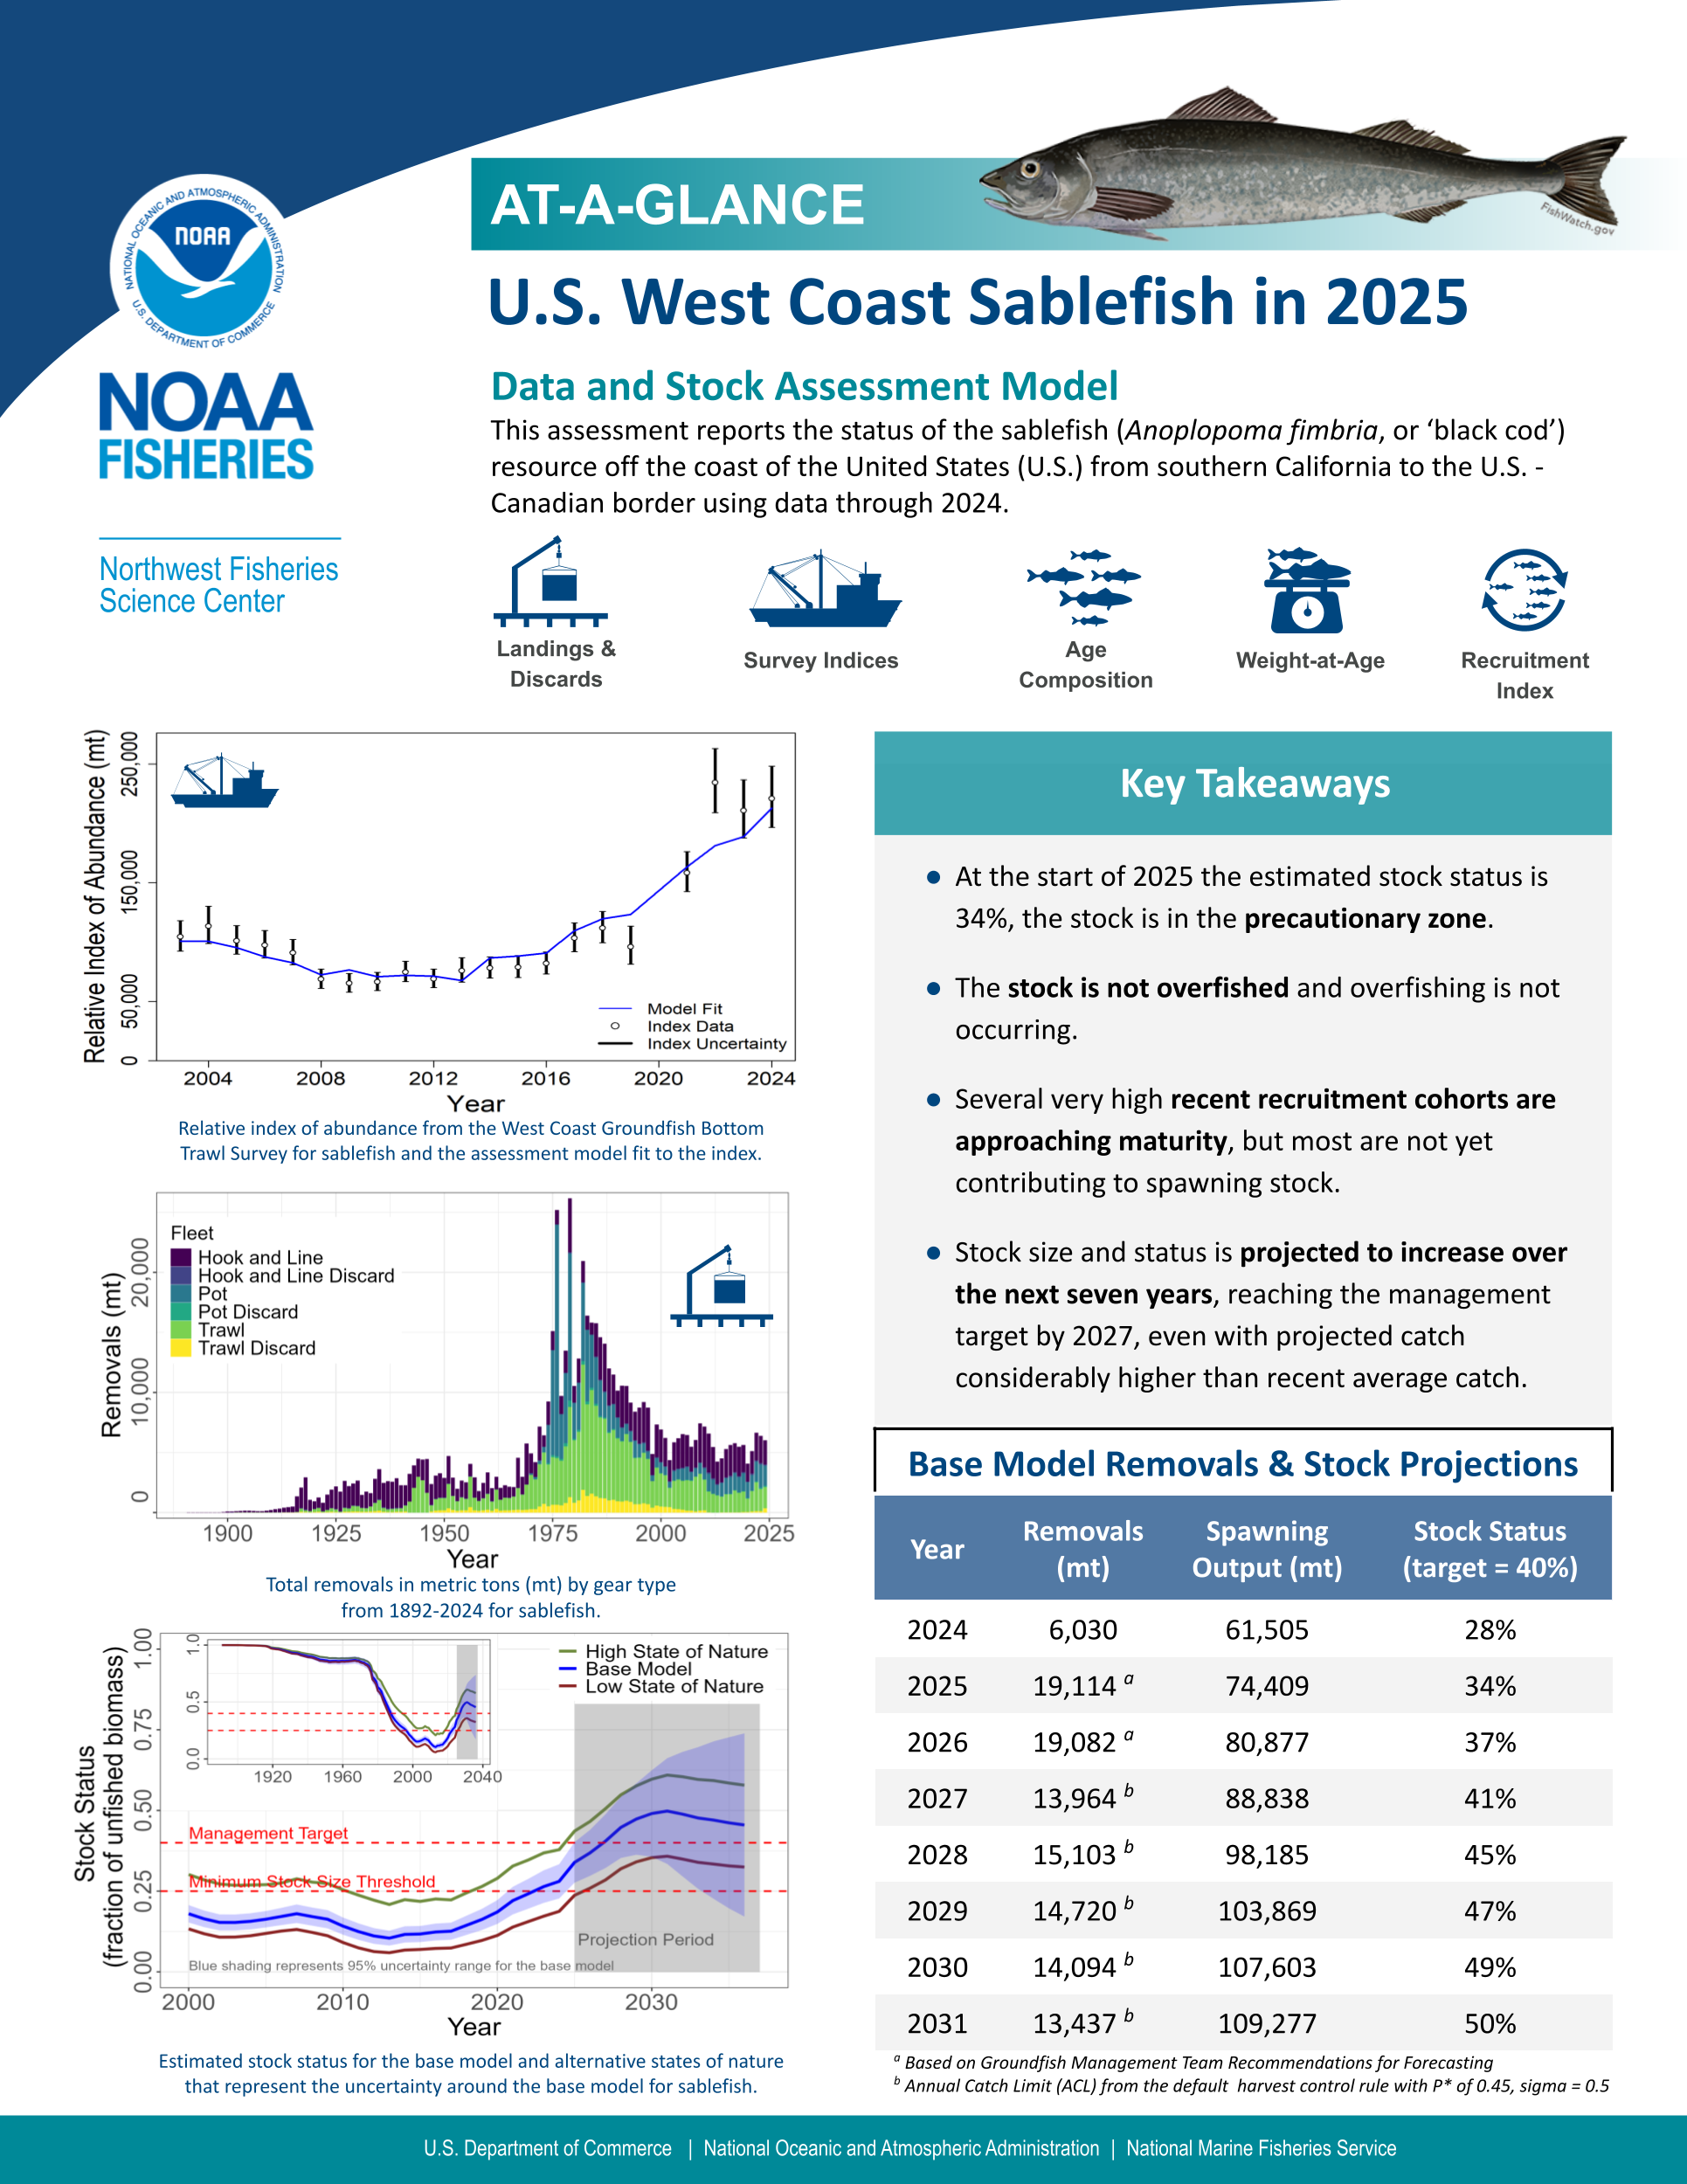
\includegraphics[width=8.5in, height=11in, alt={first page of summary graphic}]{figures/Sablefish_Stock_Overview_Fact_Sheet_2025_page_1.png}
    };
\end{tikzpicture}
\clearpage
\thispagestyle{empty}
\begin{tikzpicture}[remember picture, overlay]
    \node[inner sep=0pt, anchor=north west] 
    at (current page.north west) {
        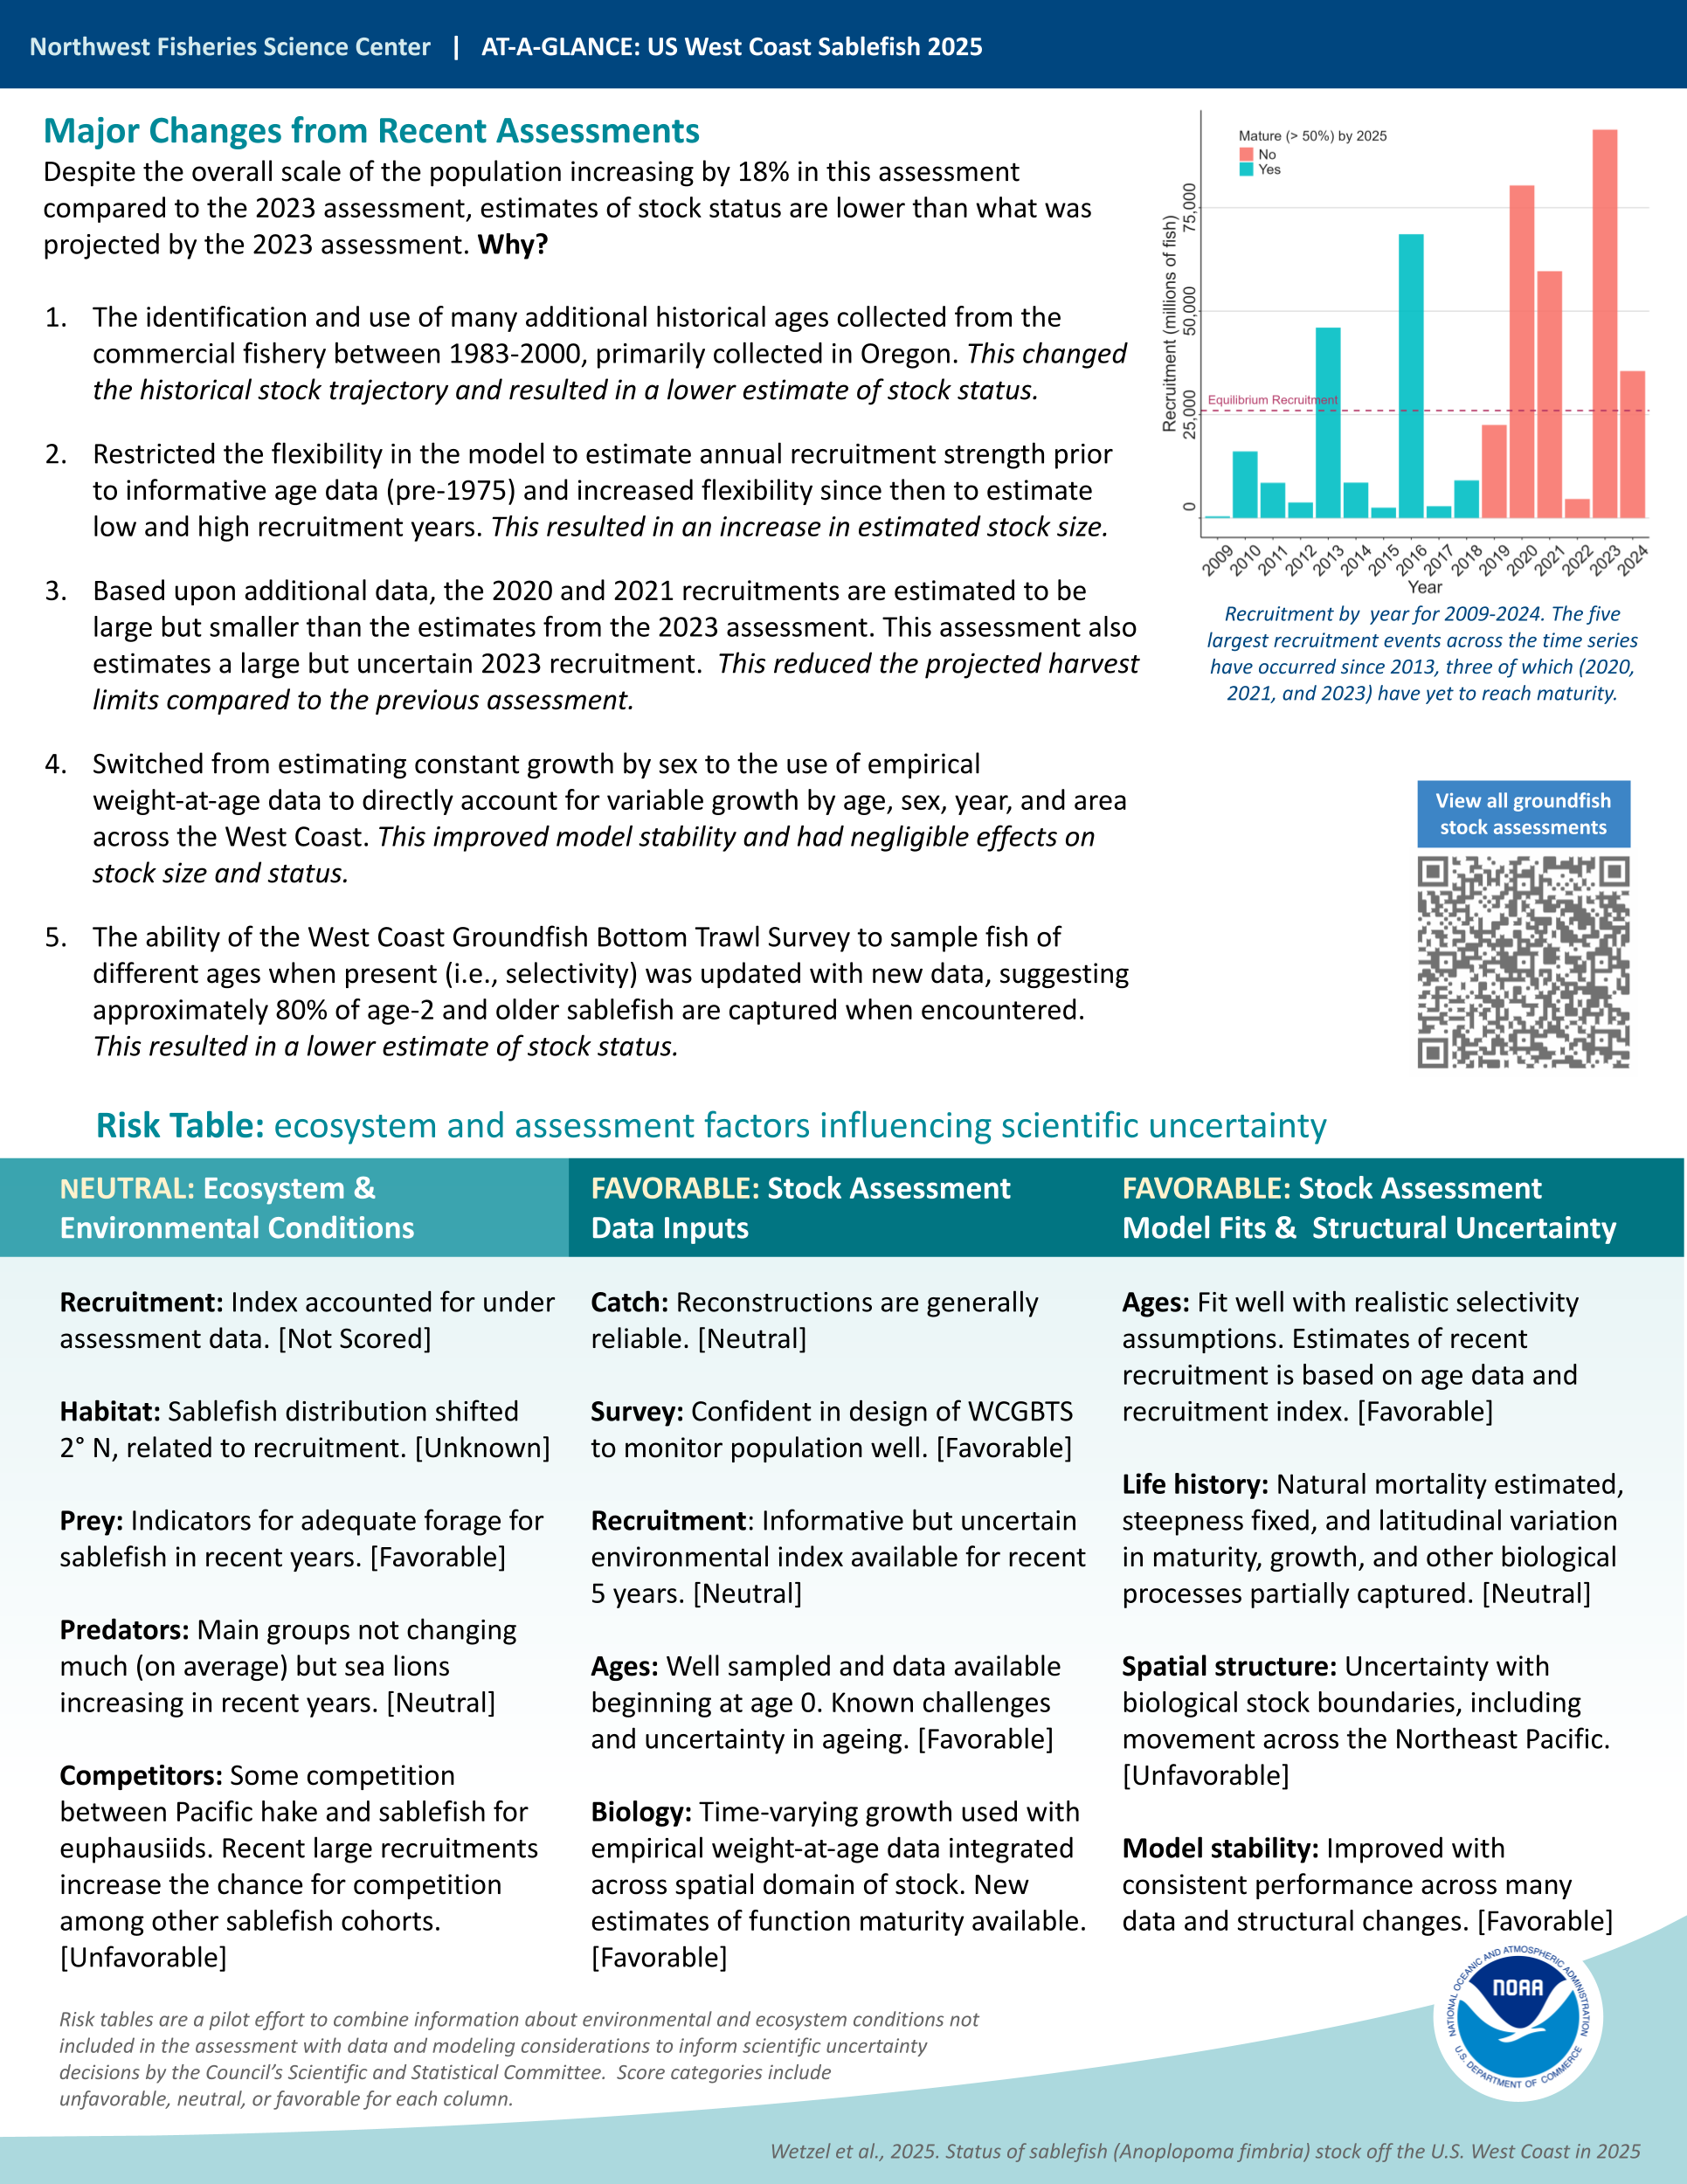
\includegraphics[width=8.5in, height=11in, alt={second page of summary graphic}]{figures/Sablefish_Stock_Overview_Fact_Sheet_2025_page_2.png}
    };
\end{tikzpicture}
\clearpage

\hypersetup{linkcolor=.}
\setcounter{tocdepth}{3}
\tableofcontents

\newpage{}

\section*{Stock Assessment Summary}\label{stock-assessment-summary}
\addcontentsline{toc}{section}{Stock Assessment Summary}

At the beginning of 2025, the population size of mature female fish
(spawning output) is estimated to be 74,409 metric tons (mt), and
overall stock status (i.e., relative spawning output compared to
unfished) is estimated to be 33.9\%. The total population (mature and
immature fish) is estimated to be sharply increasing in recent years
(nearly doubling in size since 2020) from multiple strong cohorts (e.g.,
recruitment) occurring in 2016, 2020, 2021, and 2023. The projected
coastwide Overfishing Limit (OFL) and Acceptable Biological Catch (ABC)
in 2027 are 14,935 mt and 13,965 mt, respectively. The projected
coastwide OFL and ABC in 2028 are 16,240 mt and 15,103 mt, respectively.
The projected ABC in 2027 is more than double the 2024 removals. The
2025 assessment estimates the stock status of sablefish to be lower than
what was projected by the 2023 assessment, with the population below the
management limit of 40\% and in the precautionary zone until 2027 when
stock status is projected to be greater than 40\%. However, the overall
scale of the population (\emph{SB\textsubscript{0}}) increased by 18\%
in this assessment compared to the 2023 assessment.

\emph{Why is this assessment different from the 2023 assessment?}

This assessment includes five primary improvements and changes in the
model relative to the 2023 update assessment. This includes two major
data improvements: (1) the identification and use of additional
historical ages collected from the commercial fishery between
1983--2000, primarily collected in Oregon, which led to the stock to be
estimated to be more depleted during this historical period; and (2) the
use of an improved and more transparent approach to estimate mortality
of discarded fish by the commercial fishery based upon available data
collected across fishery sectors. This new approach is considered to be
more transparent to ensure that the landings and discard mortality used
in the assessment are consistent with the values used by management in
the Groundfish Expanded Multiyear Mortality Report. Several major model
structure improvements were also made to better represent sablefish
biological processes off the West Coast. The assessment model moved to a
strict (3) data driven approach to estimate annual recruitments with
greater flexibility in the model to estimate low and high recruitment
years. The assessment model switched from estimating a static growth
function for each sex to (4) the use of empirical weight-at-age data to
account for variable growth by age, sex, year, and area across the West
Coast. Additionally, (5) the shape of the selectivity function for the
WCGBTS was updated based upon data from the survey. The survey was
estimated to have some selectivity for age-0, full selectivity for age-1
fish, and lower than one selectivity, but constant, for all older ages.
The WCGBTS is believed to consistently and representatively sample
sablefish well, covering a large majority of their habitat off the West
Coast. Many other data and model refinements were completed for this
assessment.

\newpage{}

\pagenumbering{roman}
\setcounter{page}{1}

\renewcommand{\thetable}{\roman{table}}
\renewcommand{\thefigure}{\roman{figure}}

\section*{Executive Summary}\label{executive-summary}
\addcontentsline{toc}{section}{Executive Summary}

\subsection*{Stock Description}\label{stock-description}
\addcontentsline{toc}{subsection}{Stock Description}

This assessment reports the status of the sablefish (\emph{Anoplopoma
fimbria}, or `black cod') resource off the coast of the United States
(U.S.) from southern California to the U.S.-Canadian border using data
through 2024. The resource is modeled as a single stock, however
sablefish do disperse to and from offshore sea mounts and along the
coastal waters of the continental U.S., Mexico, Canada, and Alaska and
across the Aleutian Islands to the western Pacific. Net changes in
population size or structure due to movement across the assessment
boundary are considered negligible, though alternative assumptions are
explored using sensitivity model evaluations.

\subsection*{Catches}\label{catches}
\addcontentsline{toc}{subsection}{Catches}

Removals for sablefish contains various historical domestic landings
reconstructions, historical foreign fishery catch, commercial domestic
landings, Pacific hake at-sea fishery catch estimates, and recreational
landings data. Estimated discards are included for the domestic
historical and current commercial landings using available information
on discard rates with gear-specific discard mortality rates. The model
includes six catch- or discard-based fishery fleets: trawl,
hook-and-line, pot, trawl discards, hook-and-line discards, and pot
discards. Total removals used in this assessment are shown by fleet in
Table~\ref{tbl-es-catches} and Figure~\ref{fig-es-landings}.

The earliest landings of sablefish off the U.S. West Coast used within
in this assessment begin in 1890 with hook-and-line gear. The removals
began to slowly increase starting in the 1910s and continued at a
roughly constant level until the 1960s, where removals sharply increased
due to the expansion of trawling and the use of pot gear
(Figure~\ref{fig-es-landings}). After peaking in the late 1970s, catches
slowly decreased until the 2000s when catches generally stabilized
roughly between 4,000 and 7,000 metric tons (mt) until present (see
Table~\ref{tbl-es-catches} for the most recent ten years). The pattern
of discarded sablefish across the time series was similar to catches,
though on average discard fleets caught 2 percent of the catch fleets.
Over the last 10 years, average annual catch was highest for the
hook-and-line fleet (2,204 mt), followed by the trawl (1,706 mt) and pot
(1,482 mt) fleets. Over the same period, average annual discards were
similar for trawl and hook-and-line gear (80 and 86 mt, respectively)
and was lowest for pot gear (51 mt).

\newpage{}

\begingroup
\fontsize{9.0pt}{11.0pt}\selectfont

\tagpdfsetup{table/header-rows={1}}
\begin{longtable}{>{\centering\arraybackslash}p{\dimexpr 52.50pt -2\tabcolsep-1.5\arrayrulewidth}>{\centering\arraybackslash}p{\dimexpr 52.50pt -2\tabcolsep-1.5\arrayrulewidth}>{\centering\arraybackslash}p{\dimexpr 52.50pt -2\tabcolsep-1.5\arrayrulewidth}>{\centering\arraybackslash}p{\dimexpr 52.50pt -2\tabcolsep-1.5\arrayrulewidth}>{\centering\arraybackslash}p{\dimexpr 52.50pt -2\tabcolsep-1.5\arrayrulewidth}>{\centering\arraybackslash}p{\dimexpr 52.50pt -2\tabcolsep-1.5\arrayrulewidth}>{\centering\arraybackslash}p{\dimexpr 52.50pt -2\tabcolsep-1.5\arrayrulewidth}>{\centering\arraybackslash}p{\dimexpr 52.50pt -2\tabcolsep-1.5\arrayrulewidth}}

\caption{\label{tbl-es-catches}Recent catches (mt) by fleet and total
catch (mt) summed across fleets.}

\tabularnewline

\toprule
Year & Trawl & Hook-and-Line & Pot & Trawl Discard & Hook-and-Line Discard & Pot Discard & Total Catch \\ 
\midrule\addlinespace[2.5pt]
2015 & 1,511 & 2,358 & 1,315 & 4 & 75 & 38 & 5,302 \\ 
2016 & 1,517 & 2,535 & 1,403 & 10 & 118 & 37 & 5,619 \\ 
2017 & 1,827 & 2,416 & 1,427 & 19 & 69 & 18 & 5,777 \\ 
2018 & 1,622 & 2,462 & 1,289 & 10 & 78 & 32 & 5,494 \\ 
2019 & 1,711 & 2,275 & 1,464 & 42 & 100 & 44 & 5,635 \\ 
2020 & 1,123 & 1,504 & 1,332 & 46 & 31 & 43 & 4,078 \\ 
2021 & 1,709 & 1,886 & 1,328 & 80 & 99 & 20 & 5,122 \\ 
2022 & 2,407 & 2,300 & 1,665 & 123 & 87 & 58 & 6,640 \\ 
2023 & 1,838 & 2,270 & 1,935 & 120 & 106 & 116 & 6,385 \\ 
2024 & 1,792 & 2,031 & 1,664 & 348 & 95 & 100 & 6,029 \\ 
\bottomrule

\end{longtable}

\endgroup

\begin{figure}[H]

\centering{

\includegraphics[width=1\linewidth,height=\textheight,keepaspectratio,alt={'Removals before the 1970s were less than 5,000 mt by year with landings sharply increasing in the 1970s and early 1980s and landings since ranging between approximately 5,000 to 7,500 mt by year.'}]{SAR_USWC_sablefish_skeleton_files/figure-pdf/fig-es-landings-1.pdf}

}

\caption{\label{fig-es-landings}Removals in metric tons (mt) by year for
trawl, pot, and hook-and line gears.}

\end{figure}%

\subsection*{Data and Assessments}\label{data-and-assessments}
\addcontentsline{toc}{subsection}{Data and Assessments}

The last benchmark stock assessment for sablefish took place in 2019 and
was followed by update assessments in 2021
(\citeproc{ref-kapur_status_2021}{Kapur et al. 2021}) and 2023
(\citeproc{ref-johnson_status_2023}{Johnson et al. 2023}). Changes and
additions between the 2023 update assessment and this assessment are
listed in Section \ref{changes}. This assessment used the most recent
version of the Stock Synthesis modeling platform (3.30.24). Primary data
sources include landings and age-composition data from the retained
catch. Discarded sablefish and associated age-composition data
(converted from length-compositions using a length-age key) are also
used in this assessment. Weight-at-age data are used to empirically
track changes in mean growth over time.

The relative index of abundance estimated from the National Marine
Fisheries Service (NMFS) Northwest Fisheries Science Center (NWFSC) West
Coast Groundfish Bottom Trawl Survey (WCGBTS), which includes depths
from 55--1,280 m, represents the primary source of information on the
stock's trend and was updated to include the most recent data, covering
the period 2003--2024. This assessment also uses a relative index of
abundance from the Alaska Fisheries Science Center/NWFSC Triennial Shelf
Survey, split into early (1980--1992) and late (1995--2004) periods, and
the NWFSC Slope Survey conducted from 1998--2002. Additionally, an
environmentally-driven recruitment index was incorporated into the stock
assessment to inform the most recent five years of recruitment.

The assessment is based upon a two-sex, age-structured model starting in
1890 and tracking annual changes in population dynamics up to an
accumulated population age group of 70 years. Natural mortality
(\emph{M}) was estimated and assumed to be time invariant and equal
between males and females. An empirical weight-at-age approach was
implemented with sex-specific time-varying growth between 2003--2024
that was spatially integrated on an annual basis to represent coastwide
trends in growth. Weight-at-age prior to 2003 was considered constant.
Age data were grouped by individual age classes between 0--50, with 50
being used as a data plus group. Age-based selectivity was estimated as
dome-shaped for each fleet and survey, and selectivity time blocks were
used to allow for shifts in selectivity for each fishery fleet.
Additionally, selectivity was mirrored (e.g., assumed to be the same)
between the hook-and-line and pot fleets and sex-specific. Recruitment
deviations were estimated from 1975 onwards with no restraint to sum to
zero over the main estimation time period (1975--2023). Steepness
(0.75), the standard deviation of recruitment variability (1.4), the
functional maturity schedule, and the fecundity relationship were fixed
inputs in the model. Fecundity was time-varying as the product of
time-varying weight-at-age data and a spatially-integrated maturity
schedule. The estimates of bias and uncertainty by age in age reading
(e.g., ageing error) were updated for this assessment, and summary
biomass was calculated for ages 3 plus.

The assessment was fit to data and prior information on natural
mortality by minimizing the joint negative log-likelihood. The prior for
\emph{M} assumed a log-normal distribution with a median of 0.072
yr\(^{-1}\) and a standard error of 0.31. Age composition data was
weighted by downsizing the input samples sizes for each data source
following the Francis method. Twelve year projections were conducted
that applied estimated \emph{M}, the final year (i.e., time block) for
fleet selectivity, a recent five year average weight-at-age (and
similarly fecundity), and average recruitment. A suite of data and model
structure sensitivities were conducted to examine the influence of
individual data sources and base model robustness and stability. While
base model results capture parametric uncertainty and sensitivity
evaluations explore structural uncertainty, total uncertainty is
underestimated in current stock size and status because this approach
does not account for the interaction between them or all possible
alternative model structures for sablefish population dynamics.

\subsection*{Stock Output and Dynamics}\label{stock-output-and-dynamics}
\addcontentsline{toc}{subsection}{Stock Output and Dynamics}

For the purposes of this assessment, female spawning biomass is assumed
to be proportional to egg and larval production (i.e., spawning output)
and the terms spawning biomass and spawning output are used
interchangeably through the report. Spawning output is reported in
metric tons (mt) throughout.

Overall, sablefish stock size and relative stock status have generally
declined (at different rates) over time until a recent rapid increase
due to several above average recruitment years (Table~\ref{tbl-es-sb};
Figure~\ref{fig-es-sb}). Sablefish were exploited at relatively modest
levels from the early 1900s to the mid-1970s, resulting in a gradual
decline in spawning output from the equilibrium unfished level.
Estimates of spawning output declined rapidly from the mid-1970s to the
early 2000s as a result of higher than average harvest and modest
recruitment. As annual harvest levels subsided to more moderate levels,
spawning output generally leveled off from 2000--2017 in the range of 10
to 20 percent relative stock status (below the minimum stock size
threshold; Figure~\ref{fig-es-depl}). Since 2017, spawning output is
estimated to have continually increased through 2025 to the highest
spawning output size since 1989. This rapid increase in spawning output
is due to several above average recruitment years since 2013. The
summary biomass of fish age 3 and older has a steeper increase at the
end of the time series from both the 2020 and 2021 strong cohorts.
Although the relative trend in spawning output is robust to uncertainty
in the leading model parameters, the productivity of the stock remains a
key source of uncertainty due to confounding of natural mortality,
absolute stock size, and productivity (e.g., steepness).

The estimate of 2025 female spawning output is 74,409 mt with 95 percent
asymptotic confidence intervals from 59,331 to 89,486 mt
(Table~\ref{tbl-es-sb}). The estimate of the 2025 stock status (i.e.,
the spawning output at the start 2025 divided by that at unfished
equilibrium, \emph{B\textsubscript{0}}) is 33.9 percent
(Table~\ref{tbl-es-sb}). However, the uncertainty covers 27.6 to 40.2
percent, partly due to remaining unknowns about the absolute size of
recent, potentially large, recruitment events. The estimated trajectory
of relative spawning output across the time series includes fishing the
stock down to below the minimum stock stock size threshold and then
rebounding to the precautionary zone after an extended period of reduced
harvest (relative to time series maximums) and good recruitment
(Figure~\ref{fig-es-depl}) .

\newpage{}

\begingroup
\fontsize{9.0pt}{11.0pt}\selectfont

\tagpdfsetup{table/header-rows={1}}
\begin{longtable}{>{\centering\arraybackslash}p{\dimexpr 56.25pt -2\tabcolsep-1.5\arrayrulewidth}>{\centering\arraybackslash}p{\dimexpr 56.25pt -2\tabcolsep-1.5\arrayrulewidth}>{\centering\arraybackslash}p{\dimexpr 56.25pt -2\tabcolsep-1.5\arrayrulewidth}>{\centering\arraybackslash}p{\dimexpr 56.25pt -2\tabcolsep-1.5\arrayrulewidth}>{\centering\arraybackslash}p{\dimexpr 56.25pt -2\tabcolsep-1.5\arrayrulewidth}>{\centering\arraybackslash}p{\dimexpr 56.25pt -2\tabcolsep-1.5\arrayrulewidth}>{\centering\arraybackslash}p{\dimexpr 56.25pt -2\tabcolsep-1.5\arrayrulewidth}}

\caption{\label{tbl-es-sb}Estimated recent trend in spawning output and
the stock status and the 95 percent confidence intervals.}

\tabularnewline

\toprule
Year & Spawning Output (mt) & Lower Interval (mt) & Upper Interval (mt) & Stock Status & Lower Interval & Upper Interval \\ 
\midrule\addlinespace[2.5pt]
2015 & 25,716 & 19,299 & 32,133 & 0.117 & 0.092 & 0.142 \\ 
2016 & 27,092 & 20,372 & 33,813 & 0.123 & 0.097 & 0.150 \\ 
2017 & 27,641 & 20,865 & 34,416 & 0.126 & 0.100 & 0.152 \\ 
2018 & 31,646 & 24,074 & 39,218 & 0.144 & 0.115 & 0.174 \\ 
2019 & 35,644 & 27,343 & 43,946 & 0.162 & 0.130 & 0.195 \\ 
2020 & 40,716 & 31,457 & 49,976 & 0.186 & 0.149 & 0.223 \\ 
2021 & 48,433 & 37,845 & 59,020 & 0.221 & 0.178 & 0.264 \\ 
2022 & 53,073 & 41,765 & 64,381 & 0.242 & 0.196 & 0.288 \\ 
2023 & 57,937 & 45,705 & 70,170 & 0.264 & 0.214 & 0.314 \\ 
2024 & 61,505 & 48,701 & 74,308 & 0.280 & 0.227 & 0.333 \\ 
2025 & 74,409 & 59,331 & 89,486 & 0.339 & 0.276 & 0.402 \\ 
\bottomrule

\end{longtable}

\endgroup

\begin{figure}[H]

\centering{

\includegraphics[width=1\linewidth,height=\textheight,keepaspectratio,alt={'Line plot with year on the x-axis ranging from 1890 through 2025 and spawning output on the y-axis. In 1890 spawning output is 219,377 metric tons and slowly decreases through 1975 to 178,570 metric tons, sharply decreased between 1976 to 2013 to 22,914 metric tons and slowly increases through 2025 to 74,409 metric tons.  The yearly values are available in Table 31.'}]{../model/base_model/8.36_base_model/plots/ts7_Spawning_output_with_95_intervals.png}

}

\caption{\label{fig-es-sb}Estimated time series of spawning output for
the base model.}

\end{figure}%

\begin{figure}[H]

\centering{

\includegraphics[width=1\linewidth,height=\textheight,keepaspectratio,alt={'Line plot with year on the x-axis ranging from 1890 through 2025 and stock status on the y-axis ranging from 0 to 1. Stock status slowly decreases from 1890 to 1975 to 0.814 of unfished, sharply decreased between 1976 to 2013 to 0.104, and slowly increases through 2025 to 0.339 of unfished.  The yearly values are available in Table 31.'}]{../model/base_model/8.36_base_model/plots/ts9_Fraction_of_unfished_spawning_output.png}

}

\caption{\label{fig-es-depl}Estimated time series of relative spawning
output (e.g., stock status) for the base model.}

\end{figure}%

\subsection*{Recruitment}\label{recruitment}
\addcontentsline{toc}{subsection}{Recruitment}

Sablefish recruitment is estimated to be quite variable with large
amounts of uncertainty in individual recruitment events
(Table~\ref{tbl-es-recr}; Figure~\ref{fig-es-recruits}). In general,
sablefish has low to moderate recruitment (relative to the long-term
average) with occasional large year classes (aligning with assumed high
recruitment variability: 1.4). Initial model explorations found that
there was limited information in the data to inform annual recruitment
deviations prior to 1975, so recruitment deviations were not estimated
prior to 1975 (Figure~\ref{fig-es-recdevs}).

Absolute recruitment was generally low during the 1980s--2000s when
spawning output was decreasing reaching low levels by 2000. After that
time, several average to well above average recruitment events occurred,
including the highest four recruitment events in the time series falling
between 2016--2023. Years with the highest recruitment deviations were
estimated to have occurred in 2023, 2020, 2016, 2013, and 2021. The
lowest annual recruitment deviations (e.g., negative deviations) were
estimated to have occurred in 2005, 2007, 2009, 1996, and 1992. The
estimated annual recruitment deviation in 2024 is uncertain, but
estimated to be above average based upon data from the WCGBTS and the
recruitment index. The series of large recruitment from 2013 onwards is
a major contributor to the rapid increase in spawning output and, in
particular, summary biomass (ages 3 plus) over the last 8--10 years.

\begingroup
\fontsize{9.0pt}{11.0pt}\selectfont

\tagpdfsetup{table/header-rows={1}}
\begin{longtable}{>{\centering\arraybackslash}p{\dimexpr 56.25pt -2\tabcolsep-1.5\arrayrulewidth}>{\centering\arraybackslash}p{\dimexpr 56.25pt -2\tabcolsep-1.5\arrayrulewidth}>{\centering\arraybackslash}p{\dimexpr 56.25pt -2\tabcolsep-1.5\arrayrulewidth}>{\centering\arraybackslash}p{\dimexpr 56.25pt -2\tabcolsep-1.5\arrayrulewidth}>{\centering\arraybackslash}p{\dimexpr 56.25pt -2\tabcolsep-1.5\arrayrulewidth}>{\centering\arraybackslash}p{\dimexpr 56.25pt -2\tabcolsep-1.5\arrayrulewidth}>{\centering\arraybackslash}p{\dimexpr 56.25pt -2\tabcolsep-1.5\arrayrulewidth}}

\caption{\label{tbl-es-recr}Estimated recent trend in recruitment
(1,000s) and recruitment deviations and the 95 percent confidence
intervals.}

\tabularnewline

\toprule
Year & Recruitment (1,000s) & Lower Interval (1,000s) & Upper Interval (1,000s) & Recruitment Deviations & Lower Interval & Upper Interval \\ 
\midrule\addlinespace[2.5pt]
2015 & 2,507 & 1,327 & 4,736 & -0.911 & -1.557 & -0.264 \\ 
2016 & 68,575 & 55,918 & 84,096 & 2.376 & 2.183 & 2.569 \\ 
2017 & 2,855 & 1,353 & 6,020 & -0.811 & -1.575 & -0.048 \\ 
2018 & 9,106 & 6,610 & 12,544 & 0.294 & -0.017 & 0.605 \\ 
2019 & 22,505 & 17,267 & 29,332 & 1.155 & 0.900 & 1.409 \\ 
2020 & 80,372 & 64,260 & 100,523 & 2.382 & 2.169 & 2.595 \\ 
2021 & 59,662 & 46,157 & 77,119 & 2.030 & 1.780 & 2.280 \\ 
2022 & 4,612 & 2,158 & 9,855 & -0.556 & -1.338 & 0.226 \\ 
2023 & 93,874 & 63,700 & 138,343 & 2.434 & 2.046 & 2.823 \\ 
2024 & 35,534 & 7,603 & 166,077 & 0.507 & -1.296 & 2.310 \\ 
\bottomrule

\end{longtable}

\endgroup

\begin{figure}[H]

\centering{

\includegraphics[width=1\linewidth,height=\textheight,keepaspectratio,alt={'Point plot with year on the x-axis and age 0 recruits in 1,000s on the y-axis. The highest estimated recruitment in the time series occurs in 2008, 2013, 2016, 2020, 2021, and 2023.'}]{../model/base_model/8.36_base_model/plots/ts11_Age-0_recruits_(1000s)_with_95_asymptotic_intervals.png}

}

\caption{\label{fig-es-recruits}Estimated time series of age-0 recruits
for the base model.}

\end{figure}%

\begin{figure}[H]

\centering{

\includegraphics[width=1\linewidth,height=\textheight,keepaspectratio,alt={'Point plot with year on the x-axis and recruitment deviations in log-space along y-axis. The largest positive estimated recruitment deviations in the time series occurs in 2008, 2013, 2016, 2020, 2021, and 2023. The largest negative estimated recruitment deviations in the time series occurs in 1996, 1997, 1998, 2005, 2006, and 2007. See the Report.sso file for estimates.'}]{../model/base_model/8.36_base_model/plots/recdevs2_withbars.png}

}

\caption{\label{fig-es-recdevs}Estimated time series of recruitment
deviations for the base model.}

\end{figure}%

\subsection*{Exploitation Status}\label{exploitation-status}
\addcontentsline{toc}{subsection}{Exploitation Status}

The estimated relative fishing intensity on the stock was at or above
the current management target of 1.0 from 1982 to 2018
(Table~\ref{tbl-es-spr}; Figure~\ref{fig-es-spr}). Since that time,
fishing intensity has been below 1.0, declining to 0.70 by 2024 with 95
percent asymptotic confidence intervals from 0.58 to 0.82. Here, fishing
intensity is reported as a the ratio of one minus the spawning potential
ratio to one minus the SPR target of 45 percent, or
(1-SPR)/(1-SPR\textsubscript{45\%}). The estimated exploitation rate
(catch divided by biomass of fish of age-3 and above) for the most
recent year was the lowest in the previous decade at 0.03
(Table~\ref{tbl-es-spr}). Exploitation rate has fallen faster than
relative fishing intensity in recent years because recent large
recruitments are already contributing to age 3 plus biomass
(exploitation) but have not all yet reached the age of maturity
(approximately 6 to 10 years) to contribute to spawning potential
(relative fishing intensity).

\newpage{}

\begingroup
\fontsize{9.0pt}{11.0pt}\selectfont

\tagpdfsetup{table/header-rows={1}}
\begin{longtable}{>{\centering\arraybackslash}p{\dimexpr 60.00pt -2\tabcolsep-1.5\arrayrulewidth}>{\centering\arraybackslash}p{\dimexpr 60.00pt -2\tabcolsep-1.5\arrayrulewidth}>{\centering\arraybackslash}p{\dimexpr 60.00pt -2\tabcolsep-1.5\arrayrulewidth}>{\centering\arraybackslash}p{\dimexpr 60.00pt -2\tabcolsep-1.5\arrayrulewidth}>{\centering\arraybackslash}p{\dimexpr 60.00pt -2\tabcolsep-1.5\arrayrulewidth}>{\centering\arraybackslash}p{\dimexpr 60.00pt -2\tabcolsep-1.5\arrayrulewidth}>{\centering\arraybackslash}p{\dimexpr 60.00pt -2\tabcolsep-1.5\arrayrulewidth}}

\caption{\label{tbl-es-spr}Estimated recent trend in relative fishing
intensity (1-SPR)/(1-SPR45\%), where SPR is the spawning potential
ratio, and the exploitation rate, along with the 95 percent confidence
intervals for both quantities.}

\tabularnewline

\toprule
Year & (1-SPR)/(1-SPR45\%) & Lower Interval (SPR) & Upper Interval (SPR) & Exploitation Rate & Lower Interval (Rate) & Upper Interval (Rate) \\ 
\midrule\addlinespace[2.5pt]
2015 & 1.229 & 1.101 & 1.357 & 0.068 & 0.055 & 0.081 \\ 
2016 & 1.228 & 1.097 & 1.359 & 0.052 & 0.043 & 0.062 \\ 
2017 & 1.157 & 1.020 & 1.295 & 0.054 & 0.044 & 0.064 \\ 
2018 & 1.005 & 0.866 & 1.143 & 0.052 & 0.043 & 0.062 \\ 
2019 & 0.976 & 0.838 & 1.114 & 0.038 & 0.031 & 0.044 \\ 
2020 & 0.710 & 0.584 & 0.835 & 0.027 & 0.022 & 0.032 \\ 
2021 & 0.715 & 0.594 & 0.836 & 0.033 & 0.027 & 0.039 \\ 
2022 & 0.857 & 0.728 & 0.986 & 0.042 & 0.035 & 0.050 \\ 
2023 & 0.813 & 0.684 & 0.941 & 0.031 & 0.026 & 0.037 \\ 
2024 & 0.701 & 0.581 & 0.820 & 0.027 & 0.022 & 0.032 \\ 
\bottomrule

\end{longtable}

\endgroup

\begin{figure}[H]

\centering{

\includegraphics[width=1\linewidth,height=\textheight,keepaspectratio,alt={'Line plot with year on the x-axis and relative fishing intensity on the y-axis.  The relative fishing intensity was less than 0.30 before 1968, sharply increases from 1969 to 1977, greater than 1.0 from 1977 to 2018, and the falls to just below the target from 2019 to 2025.'}]{../model/base_model/8.36_base_model/plots/SPR3_ratiointerval.png}

}

\caption{\label{fig-es-spr}Estimated time series of fishing intensity
for the base model.}

\end{figure}%

\subsection*{Ecosysystem Consideration}\label{ecosysystem-consideration}
\addcontentsline{toc}{subsection}{Ecosysystem Consideration}

The climate vulnerability analysis for the California Current
(\citeproc{ref-McClure:2023:VCC}{McClure et al. 2023a}) suggests that
processes affecting sablefish recruitment are sensitive to climatic and,
therefore, oceanic drivers. Given the high climate vulnerability of
sablefish, changes in their abundance, productivity, and spatial
distribution are likely, and these changes are in turn likely to impact
fishing fleets and communities because of the high value of this
fishery. Strong coastwide recruitment appears to be associated with good
recruitment north of Cape Mendocino (approximately 40\(^\circ\) N.
latitude), which itself is correlated with transport and temperature in
the northern portion (40\(^\circ\)--48\(^\circ\) N. latitude) of the
U.S. West Coast, specifically with the northern transport of yolk-sac
larvae (\citeproc{ref-tolimieri2018oceanographic}{Tolimieri et al.
2018}). A subsequent analysis conducted for this assessment evaluated
the relationship between a suite of environmental indicators derived
from oceanographic models and sablefish recruitment found several
predictors that explain variation around the stock--recruitment curve
(see Section \ref{rec-index-data} and Appendix \ref{rec-appendix} for
further details). These predictors were used to construct a recruitment
index, which was used in the base model to provide additional
information on the strength of recent recruitments (2020--2024). Other
environmental considerations incorporated into the assessment model as
input data directly include: the use of empirical weight-at-age data to
account for latent environmental effects on spatiotemporal growth
patterns; and the use of a spatially-integrated maturity schedule to
account for latent environmental effects on latitudinal gradients in
sablefish maturity.

Additional ecosystem and environmental considerations are explicit part
of the risk table presented at the end of the executive summary (and in
Section \ref{risk}). The 2024-2025
\href{https://www.pcouncil.org/documents/2025/02/f-1-a-cciea-report-1-2024-2025-california-current-ecosystem-status-report.pdf/}{California
Current Ecosystem Status Report} further describes the primary climate
and ocean patterns that sablefish encounter, as well as changes in
sablefish distribution, juvenile abundance indices, and trends in
sablefish primary prey and predators. The occurrence of sablefish in the
California Current has generally shifted northward over the past ten
years. Recent observed environmental and biological conditions suggest
that sablefish could be larger and closer to shore than during average
conditions.

\subsection*{Reference Points}\label{reference-points}
\addcontentsline{toc}{subsection}{Reference Points}

The \gls{pfmc} groundfish \gls{fmp} includes a \gls{hcr} based upon
general species groups that determines the \gls{ofl} and \gls{abc}. The
target, threshold, and limit reference points for sablefish as defined
by the \gls{fmp} are 40, 25, and 10 percent levels of stock status,
respectively. The \gls{ofl} is determined by the target harvest rate
based on an \gls{spr} rate of 45 percent (\(\text{SPR}_{45\%}\)). If the
stock is above the management target of 40 percent, the \gls{abc} is
equal to a fraction of the \gls{ofl} based on time-varying scientific
uncertainty (\(\sigma_y\)) and management risk tolerance (P\(^*\)). When
the stock status is below the management target and above the management
limit, the \gls{abc} is linearly reduced using the \gls{hcr} to
determine the \gls{acl}. If the stock is below the management limit, 10
percent, the \gls{acl} is set to zero. Additionally, if the stock is
estimated to be below the management threshold, 25 percent, in the year
of the assessment, a rebuilding plan is required which can set the
\(\text{SPR}\) to a fishing intensity lower than the target
\(\text{SPR}_{45\%}\).

The estimated 2025 spawning output relative to unfished of equilibrium
spawning output is 33.9 percent, below the management target of 40
percent of unfished spawning output. The fishing intensity is estimated
to be below the current management harvest rate limit
(\(\text{SPR}_{45\%}\)) at the end of the time series but is estimated
to have been above between the 1970s to the late-2010s
(Figure~\ref{fig-es-spr}). The interaction between the relative spawning
output and the ratio of the estimated \gls{spr} to the management target
(\(\text{SPR}_{45\%}\)) indicates that the stock is in the lower
quadrant indicating that the overfishing is not occurring and that
relative spawning output is below the management targets
(Figure~\ref{fig-es-spr-phase}). The current estimate of stock status is
larger than the \gls{msy}, below the \gls{spr} target and relative
target biomass reference points (Figure~\ref{fig-es-yield}).

Reference points were calculated using the estimated selectivities and
catch distributions among fleets in the final year of the model, 2025
(Table~\ref{tbl-ref-points-es}). The estimated sustainable total yield
inclusive of both landings and discards was 11,126 mt according to
\(\text{SPR}_{45\%}\). The spawning output equivalent to 40 percent of
unfished spawning output (\(\text{SB}_{40\%}\)) calculated using the SPR
target, \(\text{SPR}_{45\%}\), was 87,751 mt.

\begingroup
\fontsize{9.0pt}{11.0pt}\selectfont

\tagpdfsetup{table/header-rows={1}}
\begin{longtable}{lrrr}

\caption{\label{tbl-ref-points-es}Summary of reference points and
management quantities, including estimates of the 95 percent confidence
intervals. SO is spawning output, SPR is the spawning potential ratio,
and MSY is maximum sustainable yield.}

\tabularnewline

\toprule
Reference Point & Estimate & Lower Interval & Upper Interval \\ 
\midrule\addlinespace[2.5pt]
Unfished Spawning output & 219,377 & 183,217 & 255,537 \\ 
Unfished Age 3+ Biomass (mt) & 458,861 & 375,411 & 542,311 \\ 
Unfished Recruitment (R0) & 25,981 & 17,926 & 34,036 \\ 
2025 Spawning output & 74,409 & 59,331 & 89,486 \\ 
2025 Fraction Unfished & 0.339 & 0.276 & 0.402 \\ 
Reference Points Based SO40\% & — & — & — \\ 
Proxy Spawning output SO40\% & 87,751 & 73,287 & 102,215 \\ 
SPR Resulting in SO40\% & 0.450 & 0.450 & 0.450 \\ 
Exploitation Rate Resulting in SO40\% & 0.046 & 0.042 & 0.049 \\ 
Yield with SPR Based On SO40\% (mt) & 11,126 & 8,274 & 13,978 \\ 
Reference Points Based on SPR Proxy for MSY & — & — & — \\ 
Proxy Spawning output (SPR45) & 87,751 & 73,287 & 102,215 \\ 
SPR45 & 0.450 & — & — \\ 
Exploitation Rate Corresponding to SPR45 & 0.046 & 0.042 & 0.049 \\ 
Yield with SPR45 at SO SPR (mt) & 11,126 & 8,274 & 13,978 \\ 
Reference Points Based on Estimated MSY Values & — & — & — \\ 
Spawning output at MSY (SO MSY) & 47,863 & 40,183 & 55,543 \\ 
SPR MSY & 0.283 & 0.281 & 0.286 \\ 
Exploitation Rate Corresponding to SPR MSY & 0.079 & 0.073 & 0.085 \\ 
MSY (mt) & 12,705 & 9,423 & 15,986 \\ 
\bottomrule

\end{longtable}

\endgroup

\begin{figure}[H]

\centering{

\includegraphics[width=1\linewidth,height=\textheight,keepaspectratio,alt={'Phase plot with fraction of unfished on the x-axis and relative fishing intensity on the y-axis.  The relative fishing intensity was above the target and the fraction of unfished below the target starting in 1990 to 2018. The relative fishing intensity is below the target and the fraction of unfished below the target from 2019 to 2024.'}]{../model/base_model/8.36_base_model/plots/SPR4_phase.png}

}

\caption{\label{fig-es-spr-phase}Phase plot of fishing intensity versus
relative spawning output for the base model.}

\end{figure}%

\begin{figure}[H]

\centering{

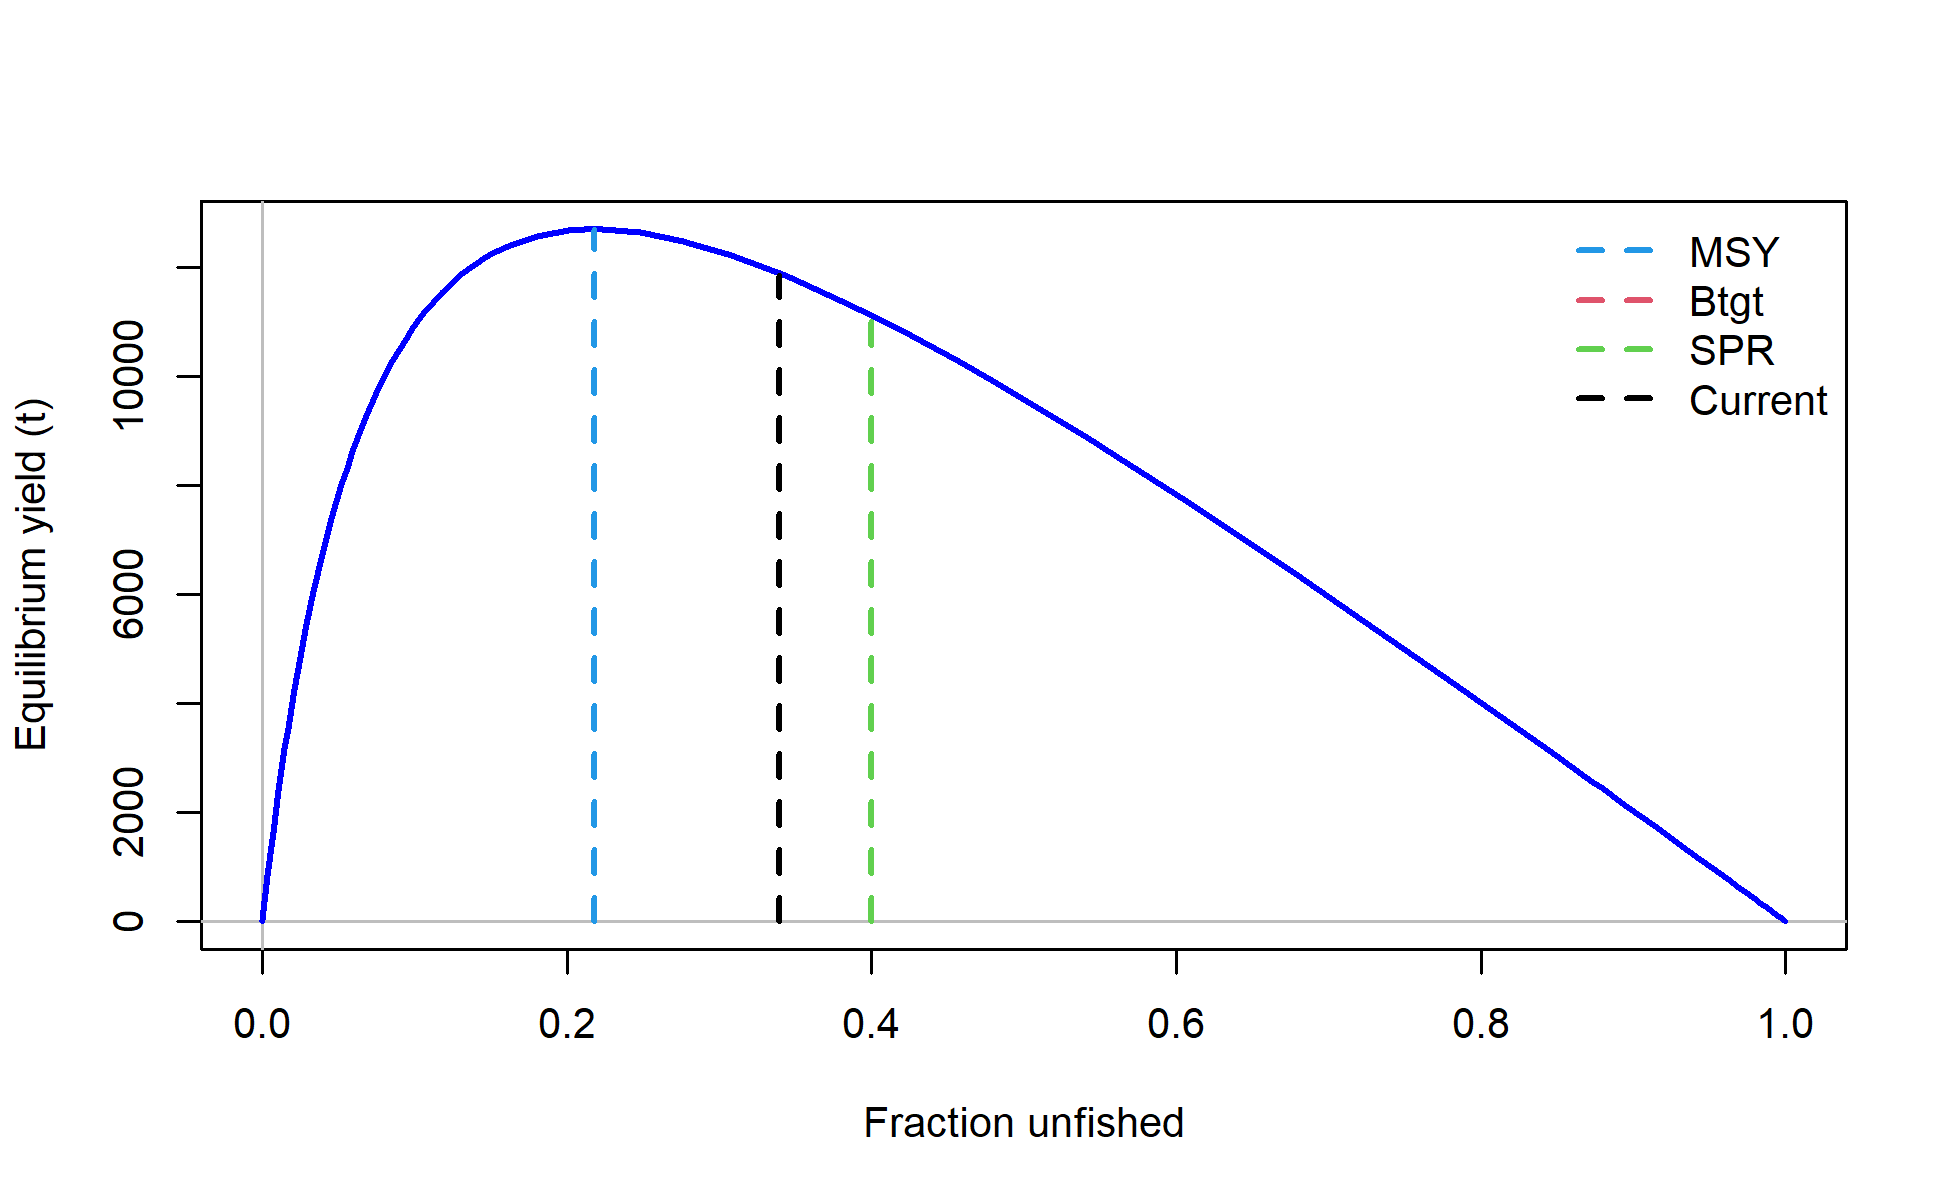
\includegraphics[width=1\linewidth,height=\textheight,keepaspectratio,alt={'Line plot with fraction of unfished on the x-axis and equilibrium yield on the y-axis. The MSY of approximately 12,705 metric tons occurs at approximately 0.22 of fraction of unfished spawning output. The equilibrium yield at the management target of 40 percent and using an SPR of 0.45 both occur at 0.44 of fraction of unfished spawning output with yield of approximately 11,126 metric tons.'}]{figures/yield2_yield_curve_with_refpoints.png}

}

\caption{\label{fig-es-yield}Estimated yield curve with reference points
for the base model. The biomass target (Btgt) and the spawning potential
ratio (SPR) target both are maximized at 0.40 fraction of unfished
spawning output.}

\end{figure}%

\subsection*{Management Performance}\label{management-performance}
\addcontentsline{toc}{subsection}{Management Performance}

Sablefish management includes a rich history of seasons, size-limits,
trip-limits, and a complex permit system. Sablefish is currently modeled
as a coastwide stock with corresponding coastwide \gls{ofl} and
\gls{abc}. The coastwide \gls{abc} is then apportioned into two
area-specific \glsplural{acl} north and south of 36\(^\circ\) N.
latitude. This historical management line corresponds with a recent
data-driven analysis of sablefish growth that suggests a difference in
growth rates north and south of \(36^\circ\) N. latitude
(\citeproc{ref-kapur_oceanographic_2020}{Kapur et al. 2020}). The
coastwide \gls{ofl} and \gls{abc} values and the area-based \gls{acl}
are shown in Table~\ref{tbl-es-management}.

For the 2019 assessment, the \gls{pfmc} adopted a methodology to
determine the area-based \gls{acl} using a five-year rolling average
relative biomass estimate from the WCGBTS
(\href{https://www.pcouncil.org/documents/2019/11/november-2019-decision-document.pdf/}{November
2019 \gls{pfmc} Meeting Decision Document}). The relative biomass
estimates represent the distribution of the sablefish population
observed by the WCGBTS, not the entire population.

The proportion of biomass observed by the WCGBTS north and south of
36\(^\circ\) N. latitude for the most recent five years is shown in
Table~\ref{tbl-es-prop-area}.

\newpage{}

\begingroup
\fontsize{9.0pt}{11.0pt}\selectfont

\tagpdfsetup{table/header-rows={1}}
\begin{longtable}{cccccc}

\caption{\label{tbl-es-management}Recent trend in the overfishing limits
(OFL), the acceptable biological catches (ABCs), the annual catch limits
(ACLs), and the total catch all in metric tons (mt).}

\tabularnewline

\toprule
Year & OFL (mt) & ABC (mt) & ACL North (mt) & ACL South (mt) & Catch (mt) \\ 
\midrule\addlinespace[2.5pt]
2015 & 7,857 & 7,173 & 4,793 & 1,719 & 5,302 \\ 
2016 & 8,526 & 7,784 & 5,241 & 1,880 & 5,619 \\ 
2017 & 8,050 & 7,350 & 5,252 & 1,864 & 5,777 \\ 
2018 & 8,239 & 7,522 & 5,475 & 1,944 & 5,494 \\ 
2019 & 8,489 & 7,750 & 5,606 & 1,990 & 5,635 \\ 
2020 & 8,648 & 7,896 & 5,723 & 2,032 & 4,078 \\ 
2021 & 9,402 & 8,791 & 6,892 & 1,899 & 5,122 \\ 
2022 & 9,005 & 8,375 & 6,566 & 1,809 & 6,640 \\ 
2023 & 11,577 & 10,825 & 8,486 & 2,338 & 6,385 \\ 
2024 & 10,670 & 9,923 & 7,780 & 2,143 & 6,029 \\ 
\bottomrule

\end{longtable}

\endgroup

\begingroup
\fontsize{9.0pt}{11.0pt}\selectfont

\tagpdfsetup{table/header-rows={1}}
\begin{longtable}{lrr}

\caption{\label{tbl-es-prop-area}Estimated percentage of sablefish
biomass estimated north and south of 36° N. latitude based on the NWFSC
West Coast Groundfish Bottom Trawl Survey data over the last five
years.}

\tabularnewline

\toprule
Year & N. 36 Latitude & S. 36 Latitude \\ 
\midrule\addlinespace[2.5pt]
2019 & 79.1\% & 20.9\% \\ 
2021 & 82.2\% & 17.8\% \\ 
2022 & 81.3\% & 18.7\% \\ 
2023 & 81.1\% & 18.9\% \\ 
2024 & 83.7\% & 16.3\% \\ 
Average & 81.5\% & 18.5\% \\ 
\bottomrule

\end{longtable}

\endgroup

\subsection*{Evaluation of Scientific
Uncertainty}\label{evaluation-of-scientific-uncertainty}
\addcontentsline{toc}{subsection}{Evaluation of Scientific Uncertainty}

The model estimated uncertainty around the 2025 spawning output for the
model is \(\sigma\) = 0.1. The uncertainty around the \gls{ofl} in 2025
is \(\sigma\) = 0.12 and the uncertainty around spawning output in 2025
is \(\sigma\) = 0.1. Each of these are likely underestimates of overall
uncertainty due to the necessity to fix several key population dynamics
parameters (e.g., steepness, recruitment variance) and also because
there is no explicit incorporation of model structural uncertainty
(although see the decision table for alternative states of nature).

\subsection*{Harvest Projections and Decision
Tables}\label{harvest-projections-and-decision-tables}
\addcontentsline{toc}{subsection}{Harvest Projections and Decision
Tables}

The projection of spawning output, stock status, and harvest limits were
developed using the base model. The total catches in 2025 and 2026 were
fixed at 19,114 and 19,082 mt, respectively, based on recommendations
from the \gls{gmt} (Table~\ref{tbl-es-gmt-catch}). The \gls{abc} values
were projected assuming a category 1 time-varying sigma with an initial
value of 0.50 in 2027 and a management risk tolerance (P\(^*\)) of 0.45.

The catches during the projection period, 2027--2037 were set equal to
the year-specific \glsplural{abc} (Table~\ref{tbl-es-projections}). The
spawning output and stock status increase during the projection due to
the estimated large recruitments in 2020, 2021, and 2023 maturing and
entering the spawning population, resulting in future \glsplural{ofl}
and \glsplural{abc}.

Two alternative catch streams based upon two options for P\(^*\), 0.45
and 0.40, were created for the decision table
(Table~\ref{tbl-es-decision-table}). Each alternative catch stream
assumes a category 1 time varying sigma with an initial value of 0.50 in
2027. The axes of uncertainty in the decision table are based on the
uncertainty around natural mortality. The low state of nature assumed a
higher natural mortality of 0.095 yr\(^{-1}\) and the high state of
nature assumed a lower natural mortality of 0.070 yr\(^{-1}\). The low
and high state of nature were run in a deterministic manner where they
assumed the same parameter values, including annual recruitment
deviations, as the base model except for natural mortality.

\begingroup
\fontsize{9.0pt}{11.0pt}\selectfont

\tagpdfsetup{table/header-rows={1}}
\begin{longtable}{>{\raggedleft\arraybackslash}p{\dimexpr 52.50pt -2\tabcolsep-1.5\arrayrulewidth}>{\raggedleft\arraybackslash}p{\dimexpr 52.50pt -2\tabcolsep-1.5\arrayrulewidth}>{\raggedleft\arraybackslash}p{\dimexpr 52.50pt -2\tabcolsep-1.5\arrayrulewidth}>{\raggedleft\arraybackslash}p{\dimexpr 52.50pt -2\tabcolsep-1.5\arrayrulewidth}>{\raggedleft\arraybackslash}p{\dimexpr 52.50pt -2\tabcolsep-1.5\arrayrulewidth}>{\raggedleft\arraybackslash}p{\dimexpr 52.50pt -2\tabcolsep-1.5\arrayrulewidth}>{\raggedleft\arraybackslash}p{\dimexpr 52.50pt -2\tabcolsep-1.5\arrayrulewidth}>{\raggedleft\arraybackslash}p{\dimexpr 52.50pt -2\tabcolsep-1.5\arrayrulewidth}}

\caption{\label{tbl-es-gmt-catch}Removal assumptions in metric tons (mt)
provided by the Groundfish Management Team for 2025-2026 by fleet.}

\tabularnewline

\toprule
Year & Trawl & HKL & Pot & Trawl Discard & HKL Discard & Pot Discard & Total Catch \\ 
\midrule\addlinespace[2.5pt]
2025 & 5,768.1 & 6,387.8 & 6,098.2 & 381.8 & 253.3 & 224.9 & 19,114.1 \\ 
2026 & 6,021.0 & 6,144.4 & 6,071.7 & 381.8 & 243.1 & 219.9 & 19,081.9 \\ 
\bottomrule

\end{longtable}

\endgroup

\begin{landscape}

\begingroup
\fontsize{9.0pt}{11.0pt}\selectfont

\tagpdfsetup{table/header-rows={1}}
\begin{longtable}{>{\centering\arraybackslash}p{\dimexpr 56.25pt -2\tabcolsep-1.5\arrayrulewidth}>{\centering\arraybackslash}p{\dimexpr 56.25pt -2\tabcolsep-1.5\arrayrulewidth}>{\centering\arraybackslash}p{\dimexpr 56.25pt -2\tabcolsep-1.5\arrayrulewidth}>{\centering\arraybackslash}p{\dimexpr 56.25pt -2\tabcolsep-1.5\arrayrulewidth}>{\centering\arraybackslash}p{\dimexpr 56.25pt -2\tabcolsep-1.5\arrayrulewidth}>{\centering\arraybackslash}p{\dimexpr 56.25pt -2\tabcolsep-1.5\arrayrulewidth}>{\centering\arraybackslash}p{\dimexpr 56.25pt -2\tabcolsep-1.5\arrayrulewidth}>{\centering\arraybackslash}p{\dimexpr 56.25pt -2\tabcolsep-1.5\arrayrulewidth}>{\centering\arraybackslash}p{\dimexpr 56.25pt -2\tabcolsep-1.5\arrayrulewidth}>{\centering\arraybackslash}p{\dimexpr 56.25pt -2\tabcolsep-1.5\arrayrulewidth}}

\caption{\label{tbl-es-projections}Potential OFLs (mt), ABCs (mt), ACLs
(mt), the buffer between the OFL and ABC, estimated spawning output
(mt),and stock status with adopted OFLs and ACLs and assumed catch for
the first two years of the projection period (2025-2026). Projections
were conducted assuming a category 1 time-varying sigma and a P\(^*\) of
0.45.}

\tabularnewline

\toprule
Year & Adopted OFL (mt) & Adopted ACL (mt) & Assumed Catch (mt) & OFL (mt) & Buffer & ABC (mt) & ACL (mt) & Spawning Output (mt) & Stock Status \\ 
\midrule\addlinespace[2.5pt]
2025 & 39,085 & 28,688 & 19,114 & — & — & — & — & 74,409 & 0.339 \\ 
2026 & 37,310 & 27,238 & 19,082 & — & — & — & — & 80,877 & 0.369 \\ 
2027 & — & — & — & 14,935 & 0.935 & 13,964 & 13,964 & 88,838 & 0.405 \\ 
2028 & — & — & — & 16,240 & 0.930 & 15,103 & 15,103 & 98,185 & 0.448 \\ 
2029 & — & — & — & 15,896 & 0.926 & 14,720 & 14,720 & 103,869 & 0.473 \\ 
2030 & — & — & — & 15,287 & 0.922 & 14,094 & 14,094 & 107,603 & 0.490 \\ 
2031 & — & — & — & 14,654 & 0.917 & 13,437 & 13,437 & 109,277 & 0.498 \\ 
2032 & — & — & — & 13,970 & 0.913 & 12,755 & 12,755 & 107,167 & 0.489 \\ 
2033 & — & — & — & 13,390 & 0.909 & 12,172 & 12,172 & 104,575 & 0.477 \\ 
2034 & — & — & — & 12,997 & 0.904 & 11,749 & 11,749 & 103,162 & 0.470 \\ 
2035 & — & — & — & 12,526 & 0.900 & 11,274 & 11,274 & 101,283 & 0.462 \\ 
2036 & — & — & — & 12,186 & 0.896 & 10,918 & 10,918 & 99,821 & 0.455 \\ 
\bottomrule

\end{longtable}

\endgroup

\end{landscape}

\tagpdfsetup{table/header-rows={1}}
\begin{table}[H]

\caption{\label{tbl-es-decision-table}Decision table summary of 10 year
projections beginning in 2027 for alternative states of nature based on
an axis of uncertainty about natural mortality for the base model.
Columns range over low, base, and high states of nature and rows range
over different catch level assumptions. The base model estimated natural
mortality of 0.088 yr\(^{-1}\) for females and males. The low state of
nature assumed a natural mortality of 0.095 yr\(^{-1}\) and the high
state of nature assumed a natural mortality of 0.070 yr\(^{-1}\) for
both sexes. Catch in 2025 and 2026 were based upon removal assumptions
provided by the GMT.}

\centering{

\centering\centering
\fontsize{9}{11}\selectfont
\begin{tabular}[t]{>{}llr>{\raggedleft\arraybackslash}p{3.75em}>{\raggedleft\arraybackslash}p{3.75em}>{\raggedleft\arraybackslash}p{3.75em}>{\raggedleft\arraybackslash}p{3.75em}>{\raggedleft\arraybackslash}p{3.75em}>{\raggedleft\arraybackslash}p{3.75em}}
\toprule
Alt. Option & Year & Catch & Low Spawning Output & Low Stock Status & Base Spawning Output & Base Stock Status & High Spawning Output & High Stock Status\\
\midrule
\textbf{P* 0.45} & 2025 & 19,114 & 45,746 & 0.237 & 74,409 & 0.339 & 136,165 & 0.436\\
\textbf{} & 2026 & 19,082 & 49,979 & 0.259 & 80,877 & 0.369 & 145,453 & \vphantom{1} 0.466\\
\textbf{} & 2027 & 13,964 & 54,904 & 0.285 & 88,838 & 0.405 & 157,818 & 0.506\\
\textbf{} & 2028 & 15,103 & 61,586 & 0.319 & 98,185 & 0.448 & 171,209 & 0.548\\
\textbf{} & 2029 & 14,720 & 65,692 & 0.341 & 103,869 & 0.473 & 179,879 & 0.576\\
\textbf{} & 2030 & 14,094 & 68,210 & 0.354 & 107,603 & 0.490 & 186,364 & 0.597\\
\textbf{} & 2031 & 13,437 & 69,067 & 0.358 & 109,277 & 0.498 & 190,326 & 0.610\\
\textbf{} & 2032 & 12,755 & 67,342 & 0.349 & 107,167 & 0.489 & 188,697 & 0.604\\
\textbf{} & 2033 & 12,172 & 65,405 & 0.339 & 104,575 & 0.477 & 186,051 & 0.596\\
\textbf{} & 2034 & 11,749 & 64,381 & 0.334 & 103,162 & 0.470 & 185,006 & 0.593\\
\textbf{} & 2035 & 11,273 & 63,290 & 0.328 & 101,283 & 0.462 & 182,588 & 0.585\\
\textbf{} & 2036 & 10,918 & 62,613 & 0.325 & 99,821 & 0.455 & 180,530 & 0.578\\
\addlinespace
\textbf{P* 0.40} & 2025 & 19,114 & 45,746 & 0.237 & 74,409 & 0.339 & 136,165 & 0.436\\
\textbf{} & 2026 & 19,082 & 49,979 & 0.259 & 80,877 & 0.369 & 145,453 & 0.466\\
\textbf{} & 2027 & 13,039 & 54,904 & 0.285 & 88,838 & 0.405 & 157,818 & 0.506\\
\textbf{} & 2028 & 14,084 & 62,010 & 0.322 & 98,644 & 0.450 & 171,704 & 0.550\\
\textbf{} & 2029 & 13,713 & 66,625 & 0.346 & 104,874 & 0.478 & 180,953 & 0.580\\
\textbf{} & 2030 & 13,115 & 69,703 & 0.362 & 109,201 & 0.498 & 188,061 & 0.602\\
\textbf{} & 2031 & 12,500 & 71,125 & 0.369 & 111,469 & 0.508 & 192,658 & 0.617\\
\textbf{} & 2032 & 11,842 & 69,855 & 0.362 & 109,844 & 0.501 & 191,566 & 0.614\\
\textbf{} & 2033 & 11,275 & 68,315 & 0.354 & 107,677 & 0.491 & 189,412 & 0.607\\
\textbf{} & 2034 & 10,880 & 67,688 & 0.351 & 106,688 & 0.486 & 188,863 & 0.605\\
\textbf{} & 2035 & 10,407 & 66,935 & 0.347 & 105,159 & 0.479 & 186,863 & 0.599\\
\textbf{} & 2036 & 10,045 & 66,586 & 0.345 & 104,029 & 0.474 & 185,201 & 0.593\\
\bottomrule
\end{tabular}

}

\end{table}%

\subsection*{Unresolved Problems and Major
Uncertainties}\label{unresolved-problems-and-major-uncertainties}
\addcontentsline{toc}{subsection}{Unresolved Problems and Major
Uncertainties}

The base model was developed with the goal of balancing parsimony with
realism and fitting the data well. To achieve parsimony, some
simplification of model structure was assumed which may have a moderate
impact on the interpretation and fit to specific data sets. The base
model was developed with a focus on stability which supports model
development, interpretability, and future update assessments. This
assessment estimates a sharp increase in young sablefish biomass and
future data collected by the WCGBTS should be monitored potential
changes in the population trajectories.

The estimated increase in young sablefish biomass is being driven by
very large recruitment events occurring in recent years (e.g., 2020,
2021, and 2023). There have been multiple observations of the 2020 and
2021 year class and appear to be well estimated by the model. However,
there is more uncertainty around the 2023 year class given the limited
observations in the data by the the WCGBTS and the fishery fleets. The
uncertainty around the strength of this year class will be resolved with
future observations by the survey and the fishery.

The patterns observed in historical sablefish recruitment suggest that
the stock trajectory, which is dominated by shifts in recruitment
strength, is closely linked to productivity regimes in the California
Current. Studies of oceanographic drivers of sablefish recruitment
explain some portion of recruitment variability for sablefish, depending
upon the oceanographic covariates evaluated. Uncertainty in future
environmental conditions and changes in the timing, dynamics, and
productivity of the California Current ecosystem via climate change or
cycles similar to the historical period should be considered as a
significant source of uncertainty in all projections of stock status.
The ongoing WCGBTS is a fairly precise relative index of abundance over
a broad demographic component of the stock but it does not survey the
entire stock as sablefish reside in waters deeper than 1,280 m and to
the north and south of the survey extent. Therefore, a portion of the
stock is unobserved. This index has the potential to inform future stock
assessments about the scale of the population relative to catches being
removed; however, such information will require contrast in the observed
survey trend.

Sablefish appear to have variable maturity-at-age latitudinally across
the U.S. West Coast. Additionally, there appears to be variable growth
spatially and temporally. This assessment attempts to account for these
variations by using a empirical weight-at-age approach that accounts for
space and time. In the available data, there were not clear trends
across time but rather periods of above or below average growth. Future
data should continue to be evaluated for potential trends in growth and
maturity and whether those observed patterns vary from what was assumed
in this assessment.

\subsection*{Research and Data Needs}\label{research-and-data-needs}
\addcontentsline{toc}{subsection}{Research and Data Needs}

Most of the research needs listed below entail investigations that need
to take place outside of the routine assessment cycle and require
additional resources to be completed.

\begin{enumerate}

\item Spatiotemporal distribution patterns with depth: There are patterns of age and sex
ratios with depth which may indicate that the stock is more complex than currently
modeled. Further research into the causes of these patterns as well as differences
between seasons would help with understanding the stock characteristics such that
a more realistic model could be built if needed. This may also provide further insight into
migration and help determine if there are localized populations.

\item Stock boundaries: A common question in stock assessments is whether or not the
entire stock is being represented. Sablefish live deeper than the range of the fisheries
and surveys off the U.S. West Coast. The assessment model attempts to account for out of area biomass
through catchability coefficients and selectivity curves, but that portion of the stock is
unknown and can only be conjectured. Research into abundance in deep areas would
be useful to verify that the assessment adequately predicts the entire stock
of sablefish. In addition, sablefish along the U.S. West Coast can move northward to
Canada or Alaska management jurisdictions. Building on recent transboundary sablefish research
(Kapur et al. 2024, Kapur et al. in press), investigations elucidating how variable movements (net
emigration and immigration) are from year to year to better understand impacts on current
management advice or, ultimately, incorporate these changes into stock assessment models.

\item Recruitment: Continued investigation and refinement of environmental covariates for
recruitment on a stock-wide, northeast Pacific scale. Continued evaluations into the estimation
of steepness ($h$) is warranted in future stock assessments 

\item Stock trends: The WCGBTS is a critical data source in this assessment providing data
about the age distribution of the stock, incoming recruitment with observations of age-0 fish, and
an informative trend in biomass. Continuation of the annual WCGBTS will provide information
on stock trends and incoming recruitments. A longer survey time series may improve the precision of
estimates of absolute stock size and productivity into the future. This is particularly true now that
the stock has had substantial contrast (declines and inclines) in stock biomass, catch, and
recruitment dynamics. 

\item Ageing: Age validation is needed to verify the level of age bias present in the data, if any.
The assessment model now uses empirical weight-at-age data to track spatiotemporal variation in growth.
The continuation of collecting representative otolith samples and fish weights from fishery-independent and fishery-dependent
sources, and processing those samples for age determination, is required to continue including time-varying
growth into the assessment model. Continued research and pilot applications using Fourier Transform
Near-Infared Spectroscopy (FT-NIRS) methods for ageing, which includes an understanding of the potential
benefits (e.g., increase age determination throughput and efficiency) and barriers (e.g., bias)
specific to sablefish could help to achieve ongoing ageing goals given competing demands for available
resources. In addition, there is an under-representation of ages from sablefish caught in fisheries off of California
compared to other areas. Biological sampling designs should strive to be consistent across the stock domain.

\item Fish Weight: This assessment uses an empirical weight-at-age approach to account for spatially and time varying growth informed by data from the WCGBTS. Currently, fish weight information is not available coastwide commercial fisheries (e.g., information available in PacFIN).  Collected and reporting fish weight information to port sampling coastwide would support the consideration of commercial fishery data to understand weight-at-age of sablefish for future assessments. 

\item Temporal and spatial biology: Research on understanding the interactions between spatial patterns in
sablefish growth, maturity, and natural mortality across space and time will provide important information for future assessments.
Both growth and maturity show latitudinal trends across the stock domain. While the current assessment
accounts for these trends in the pre-processing of the data provided to the assessment model, it does so in a limited way.
While tracking spatiotemporal changes in natural mortality by sex or life-stage is difficult, often requiring data
that is unavailable (e.g., extensive tagging data), there has been recent advances through the use of external
ecosystem modeling approaches such as the Climate- Enhanced, Age-based model with Temperature-specific Trophic
Linkages and Energetics (CEATTLE) that should be explored for sablefish.

\end{enumerate}

\subsection*{Risk Table}\label{risk-table}
\addcontentsline{toc}{subsection}{Risk Table}

Oceanographers and stock assessment scientists jointly constructed a
risk table to identify the main ecosystem and environmental processes
for sablefish that should be considered in conjunction with available
data used in the stock assessment and the structural uncertainty
embedded in the assessment (Table~\ref{tbl-risk-table-es}). The group
considered ecosystem and environmental indicators for sablefish
recruitment, habitat, prey, predators, competitors, and the recent
climate vulnerability assessment
(\citeproc{ref-McClure:2023:VCC}{McClure et al. 2023a}). Overall, the
group considered these conditions to generally be neutral (Level 2) when
considering, among other things, unresolved uncertainty with linkages
between trends in primary predators and competitors and a overall
climate vulnerability score of moderate. Data inputs for sablefish were
scored as favorable (Level 1) given confidence in historical catch
reconstructions, a comprehensive and representative survey index of
abundance (WCGBTS), well sampled age data beginning at age zero, an
informative recruitment index, and information on time- (growth) and
-spatially-varying (maturity) life history characteristics across the
stock range. The ability for the stock assessment model to fit the data
and capture key sources of structural uncertainty was also scored as
favorable (Level 1). Despite the need to fix certain productivity
parameters (e.g., steepness and recruitment variability) or simplify
some assumptions (e.g., sex invariant \emph{M} and no net loss from
emigration or immigration), model complexity seemed to balance well
potential bias and variance in a way that stabilized sablefish
population dynamics across a wide breadth of alternative data and model
structures (see Section \ref{sensitivities} for sensitivity
evaluations).

\newpage{}

\begingroup
\fontsize{6.0pt}{7.0pt}\selectfont

\tagpdfsetup{table/header-rows={1}}
\begin{longtable}{>{\raggedright\arraybackslash}p{\dimexpr 142.50pt -2\tabcolsep-1.5\arrayrulewidth}>{\raggedright\arraybackslash}p{\dimexpr 142.50pt -2\tabcolsep-1.5\arrayrulewidth}>{\raggedright\arraybackslash}p{\dimexpr 142.50pt -2\tabcolsep-1.5\arrayrulewidth}}

\caption{\label{tbl-risk-table-es}Risk table for sablefish to document
ecosystem and environmental factors potentially affecting stock
productivity and uncertainty or other concerns arising from the stock
assessment. Level 1 is a favorable ranking, Level 2 neutral, and Level 3
unfavorable.}

\tabularnewline

\toprule
Ecosystem and Environmental Conditions & Assessment Data Inputs & Assessment Model Fits and Structural Uncertainty \\ 
\midrule\addlinespace[2.5pt]
• Recruitment: Recent strong recruitment is considered under the assessment data inputs. [Not Scored] & • Catch reconstructions (landings and
discards) date back to the early 1900s for hook-and-line and trawl fisheries. Foreign landings records began in the 1960s. [Neutral] & • Length data were available but no used in the model [Neutral] \\ 
 &  &  \\ 
• Habitat: The center of gravity for sablefish biomass has shifted approximately 2° northward in recent years. [Unknown]  & • There is high confidence in the primary fishery-independent survey (WCGBTS). Sablefish also occur deeper than the survey samples. [Favorable] & • Age data generally fit well with realistic selectivity assumptions. Estimates of recent large cohorts were robust across sensitivity runs. The model estimates recent recruitments based on age data and the recruitment index. [Favorable]  \\ 
 &  &  \\ 
• Prey: Increased euphausiid and juvenile hake biomass suggest adequate prey availability for sablefish in recent years. [Favorable] & • An informative but highly uncertain environmentally driven recruitment index was incorporated into the assessment for the most recent 5 years. [Neutral] & • Natural mortality was estimated but assumed to be constant for all life stages and across time and space. Natural mortality was set to be equal by sex based upon similar model estimates. [Neutral] \\ 
 &  &  \\ 
• Predators: Sablefish consumption (by California sea lions, sperm whales, porpoises, skates, and fur seals) is unlikely to have changed in recent years, but there have been long-term increases in the abundance of some groups like sea lions. [Neutral] & • Age data have been relatively well sampled. The WCGBTS provides coastwide age data and ages are available from the fishery for the last 40 years but lack coastwide sampling in recent years. Data to inform recent recruitment is well represented. There are known challenges and uncertainty in ageing. [Favorable] & • Steepness was fixed (h = 0.75) given life history and management (reference point) objectives. Available data are not informative of absolute stock size or productivity at small stock sizes. [Neutral]  \\ 
 &  &  \\ 
• Competition: There is potential for competition between sablefish and Pacific hake (e.g., for euphausiids). Changes in competitive interactions are highly uncertain given limited information about prey availability and spatiotemporal overlap with potential competitors. Recent large recruitments increase the likelihood of intraspecific, density-dependent, competition. [Unfavorable] & • Time-varying growth relies on empirical weight-at-age and is integrated across latitudes according to survey biomass. [Favorable] & • There is variation in maturity, growth, and potentially other biological processes across the latitudinal range that is partially captured in the model. [Neutral] \\ 
 &  &  \\ 
 & • Spatially explicit estimates of functional maturity account for latitudinal differences in productivity. [Favorable] & • There is uncertainty with respect to biological stock boundaries, including movement across the Northeast Pacific. [Unfavorable]  \\ 
 &  &  \\ 
 &  & • Extensive sensitivity runs produced reasonable results and changes were generally similar relative to base model results. There were little to no retrospective patterns or other diagnostic issues. The model produces stable jitters and parameter estimates that did not considerably vary by data source or as a result of structural changes. [Favorable] \\ 
 &  &  \\ 
Level 2: Neutral & Level 1: Favorable & Level 1: Favorable \\ 
\bottomrule

\end{longtable}

\endgroup

\newpage{}

Accounting for each factor considered in the risk table, the overall
conditions for sablefish is currently considered favorable which could
support the application of scientific uncertainty (\(\sigma\)) lower
than the default (\(\sigma\) of 0.50) for a category one assessment for
projecting future harvest specifications.
Table~\ref{tbl-es-risk-table-projections} shows an theoretical
projection using a \(\sigma\) of 0.25 and a P* of 0.45 that could be
considered if the use of risk tables is adopted by management for future
stock assessments and a \(\sigma\) of 0.25 is deemed appropriate by the
Scientific and Statistical Committee.

\begingroup
\fontsize{9.0pt}{11.0pt}\selectfont

\tagpdfsetup{table/header-rows={1}}
\begin{longtable}{>{\centering\arraybackslash}p{\dimexpr 52.50pt -2\tabcolsep-1.5\arrayrulewidth}>{\centering\arraybackslash}p{\dimexpr 52.50pt -2\tabcolsep-1.5\arrayrulewidth}>{\centering\arraybackslash}p{\dimexpr 52.50pt -2\tabcolsep-1.5\arrayrulewidth}>{\centering\arraybackslash}p{\dimexpr 52.50pt -2\tabcolsep-1.5\arrayrulewidth}>{\centering\arraybackslash}p{\dimexpr 52.50pt -2\tabcolsep-1.5\arrayrulewidth}>{\centering\arraybackslash}p{\dimexpr 52.50pt -2\tabcolsep-1.5\arrayrulewidth}>{\centering\arraybackslash}p{\dimexpr 52.50pt -2\tabcolsep-1.5\arrayrulewidth}>{\centering\arraybackslash}p{\dimexpr 52.50pt -2\tabcolsep-1.5\arrayrulewidth}}

\caption{\label{tbl-es-risk-table-projections}Theoretical OFLs (mt),
ABCs (mt), ACLs (mt), the buffer between the OFL and ABC, estimated
spawning output, stock status, and assumed catch for the first two years
of the projection period (2025-2026). Projections were conducted
assuming a time-varying sigma of 0.25 and a P\(^*\) of 0.45.}

\tabularnewline

\toprule
Year & Assumed Catch (mt) & OFL (mt) & Buffer & ABC (mt) & ACL (mt) & Spawning Output (mt) & Stock Status \\ 
\midrule\addlinespace[2.5pt]
2025 & 19,114 & — & — & — & — & 74,409 & 0.339 \\ 
2026 & 19,082 & — & — & — & — & 80,877 & 0.369 \\ 
2027 & — & 14,935 & 0.967 & 14,442 & 14,442 & 88,838 & 0.405 \\ 
2028 & — & 16,209 & 0.965 & 15,642 & 15,642 & 97,948 & 0.446 \\ 
2029 & — & 15,832 & 0.962 & 15,230 & 15,230 & 103,345 & 0.471 \\ 
2030 & — & 15,194 & 0.960 & 14,586 & 14,586 & 106,779 & 0.487 \\ 
2031 & — & 14,537 & 0.958 & 13,926 & 13,926 & 108,155 & 0.493 \\ 
2032 & — & 13,835 & 0.955 & 13,212 & 13,212 & 105,795 & 0.482 \\ 
2033 & — & 13,240 & 0.953 & 12,618 & 12,618 & 102,992 & 0.469 \\ 
2034 & — & 12,834 & 0.951 & 12,205 & 12,205 & 101,373 & 0.462 \\ 
2035 & — & 12,353 & 0.949 & 11,723 & 11,723 & 99,311 & 0.453 \\ 
2036 & — & 12,003 & 0.947 & 11,367 & 11,367 & 97,677 & 0.445 \\ 
\bottomrule

\end{longtable}

\endgroup

\newpage{}

\setlength{\parskip}{5mm plus1mm minus1mm}
\pagenumbering{arabic}
\setcounter{page}{1}
\setcounter{section}{0}
\renewcommand{\thefigure}{\arabic{figure}}
\renewcommand{\thetable}{\arabic{table}}
\setcounter{table}{0}
\setcounter{figure}{0}

\section{Introduction}\label{introduction}

\subsection{Stock Description}\label{stock-description-1}

Sablefish (\emph{Anoplopoma fimbria}, also known as black cod) are
distributed in the northeastern Pacific Ocean from the southern tip of
Baja California northward to the north-central Bering Sea and in the
northwestern Pacific Ocean from Kamchatka southward to the northeastern
coast of Japan (\citeproc{ref-hart_pacific_1973}{Hart 1973};
\citeproc{ref-eschmeyer_field_1983}{Eschmeyer and Herald 1983}). U.S.
West Coast sablefish are modeled as a single stock. Thus, this stock
assessment does not explicitly account for movement between offshore sea
mounts (\citeproc{ref-shaw_movement_1997}{Shaw and Parks 1997};
\citeproc{ref-morita_sex_2012}{Morita et al. 2012};
\citeproc{ref-hanselman_move_2015}{Hanselman et al. 2015}), regions to
the north or south of the U.S. West Coast, or to the western Pacific
(\citeproc{ref-fujioka_description_1988}{Fujioka et al. 1988};
\citeproc{ref-heifetz_movement_1991}{Heifetz and Fujioka 1991};
\citeproc{ref-hanselman_move_2015}{Hanselman et al. 2015}). The area
included in this assessment is shown in Figure~\ref{fig-map}.

Previous analyses suggest the existence of several stocks of sablefish
in the eastern Pacific Ocean that are largely delineated by management
boundaries (Schirripa (\citeproc{ref-schirripa_sablefish_2007}{2007a});
and earlier assessments), though more recent genetic analyses found that
sablefish in the northeastern Pacific Ocean are a single panmictic
population (\citeproc{ref-jasonowicz_love_2017}{Jasonowicz et al.
2017}). Additional support for a panmictic population stems from tag
recoveries that show sablefish move across international boundaries,
including regions currently used for management
(\citeproc{ref-kapur_tag_2025}{Kapur et al. in press};
\citeproc{ref-hanselman_move_2015}{Hanselman et al. 2015};
\citeproc{ref-sogard_patterns_2017}{Sogard and Berkeley 2017}). Despite
generally similar movement estimates between the U.S. West Coast and
British Columbia, a net change in demography may still be present due to
differences in area-specific population sizes
(\citeproc{ref-kapur_range_2024}{Kapur et al. 2024}). Analyses of
length-at-age data have found spatial variation in von Bertalanffy
growth parameters across the northeastern Pacific Ocean
(\citeproc{ref-mcdevitt_status_1987}{McDevitt 1987a};
\citeproc{ref-echave_interdecadal_2012}{Echave et al. 2012a};
\citeproc{ref-head_maturity_2014}{Head et al. 2014};
\citeproc{ref-gertseva_spatial_2017}{Gertseva et al. 2017};
\citeproc{ref-kapur_oceanographic_2020}{Kapur et al. 2020}). Geographic
break points at approximately (1) 36\(^\circ\) N. latitude between Point
Conception and Monterey, California and (2) 50\(^\circ\) N. latitude
where the North Pacific Current bifurcates suggest zones of growth
variation. However, increasing maximum body size and decreasing relative
growth rates with increasing latitude do not indicate regions with
separate populations.

Smaller sablefish are generally found in shallower waters, but the
demographics appear to be fully mixed (adult and juvenile) near the
shelf-slope break (i.e., 100--300 m). Beyond the shelf-slope break, the
population is dominated by older individuals
(\citeproc{ref-methot_assessment_1994}{Methot 1994a}) and younger fish
become increasingly rare. Fish in the deepest areas sampled tend to be
the oldest but not the largest individuals, suggesting that age dictates
depth-specific distributions. The interaction between environmental
conditions and seasonal movements that produce an increase in age with
depth are largely unknown. The stock is distributed beyond the greatest
depths sampled by any of the surveys and beyond the deepest commercial
fishing areas. Research in the deeper habitats occupied by sablefish is
potentially difficult because they extend across the boundary of the
exclusive economic zone and near sea mounts and ridges across the
Pacific Ocean. The population of sablefish in the Puget Sound and Strait
of Georgia is negligible compared to that in coastal U.S. waters.
Therefore, connectivity among these areas and the open coast is likely
of less importance to this stock assessment than movement along the
coast.

\subsection{Life History}\label{life-history}

Tolimieri et al. (\citeproc{ref-tolimieri2018oceanographic}{2018})
provide a thorough review of the literature on spawning and early life
history of sablefish in the California Current. Briefly, sablefish off
the U.S. West Coast spawn along the continental shelf-slope break in
waters deeper than 300 m and exhibit a protracted spawning period from
December through March, with peak activity in February
(\citeproc{ref-guzman_reproductive_2017}{Guzmán et al. 2017}). Spawning
in deeper waters may result in reduced availability to the commercial
fishery during the winter months. Pelagic juveniles are present in
off-shore surface waters and settle to the benthos as age-0 recruits
during the late summer and fall, with most newly settled fish observed
at depths less than 250 m.

Sablefish mature between 5-11 years
(\citeproc{ref-head_maturity_2014}{Head et al. 2014}). Female sablefish
generally reach larger sizes than males. The sex-ratio tends to be
skewed toward males at the oldest ages, implying higher fishing pressure
on females or/and a lower natural mortality rate for males. The oldest
sablefish observed off the West Coast as captured off Washington in 2006
and aged (with observation error) at 102 years.

Adult sablefish are fast-swimming and capable of feeding on a diverse
array of prey species including fishes, cephalopods, and crustaceans
(\citeproc{ref-low_sablefish_1976}{Low et al. 1976}). The cohabitation
of adult and juvenile sablefish may result in some cannibalism. The
large changes in predator biomass could have a negative effect on
juvenile survival and, therefore, stock productivity.

\subsection{Ecosystem Considerations}\label{ecosystem-considerations}

The sablefish \gls{cva} suggests that processes affecting recruitment
are sensitive to environmental drivers
(\citeproc{ref-mcclure_2023_vulnerability}{McClure et al. 2023b}).
Climate-driven changes in the abundance, productivity, and spatial
distribution of sablefish are likely and can have considerable impacts
to fishing fleets and communities because of the high value of this
fishery.

The sablefish stock has experienced latitudinal shifts in the center of
the distribution of stock biomass within the California Current, which
has affected fishing opportunities to individual ports
(\citeproc{ref-selden_2019}{Selden et al. 2019}). The population
centroid shifted to the north from 1980 to 1992, to the south by 2013,
and back to the north in recent years, illustrated by an increase in
\gls{s-wcgbt} biomass estimates.

Strong coast-wide recruitment appears to be associated with strong
recruitment north of Cape Mendocino (\textasciitilde{} 40\(^\circ\) N.
latitude). Strong recruitment is correlated with larval transport and
temperature in the northern portion of the U.S. West Coast
(40\(^\circ\)--48\(^\circ\) N. latitude)
(\citeproc{ref-tolimieri2018oceanographic}{Tolimieri et al. 2018}).
Variation around the stock-recruitment curve was negatively correlated
with sea level north of Cape Mendocino, CA. The 2019 assessment of
sablefish included a sea surface height index within the model to inform
historical and recent recruitment
(\citeproc{ref-haltuch_status_2019}{Haltuch et al. 2019}). This
assessment includes a revised recruitment index that accounts for
several oceanographic and ecosystem variables that appear to be
correlated with sablefish recruitment in recent years (see Section
\ref{rec-index-data} for additional information).

Age-0 sablefish captured by the \gls{s-wcgbt} were most abundant in
shelf and upper-slope waters around San Francisco Bay and from Cape
Mendocino to the Columbia River. The abundance of age-0 recruits varied
through time with peaks in recruitment in 2008, 2013, 2016, 2020, 2021,
and 2023. Most strong recruitment years were associated with high
recruitment north of Cape Mendocino. Recent modeling work suggests that
strong age-0 recruitment is associated, in part, with the northward
transport of yolk-sac larvae at depths between 1,000--1,200 m
(\citeproc{ref-tolimieri2018oceanographic}{Tolimieri et al. 2018}),
which may lead to greater spatiotemporal overlap between feeding larvae
and copepod prey than when larval transport is not as well defined.

\subsection{Fishery Description}\label{fishery-description}

Historical sablefish landings, beginning in 1890, have been
reconstructed by the states (Washington, Oregon, and California) using a
variety of sources. Generally, historical sablefish landings were more
reliable than those for many other groundfish species because of
consistent species-level identification. Although sablefish landings
were recorded at the start of the 20th century, appreciable quantities
were not landed until 1916--1919, with landings remaining below 5,000 mt
through the late 1960s. Landings prior to 1960 were primarily harvested
by hook-and-line gear.

Sablefish landings increased dramatically during the 1970s, first from a
combination of foreign vessels
(\citeproc{ref-lynde_historical_1986}{Lynde 1986};
\citeproc{ref-mcdevitt_status_1987}{McDevitt 1987a}), followed by an
increase in the domestic fleet. Increases in catch correspond to the
introduction of a pot fishery, followed by the trawl sector, with only
minor increases in hook-and-line catches until the mid-1980s. Over
25,000 mt of sablefish were removed in 1976 and 1979 from U.S. West
Coast waters. A rapid increase in domestic pot and trawl landings
followed these peak removals, with slow declines from \textasciitilde{}
19,000 mt in 1982 to \textasciitilde{} 9,000 mt in 1990. This decline in
domestic landings was likely due to a combination of declining stock
size, reduced Asian-market strength, and stricter fishery regulations.
Annual landings have remained below 6,500 mt over the past decade, with
approximately 43 percent of removals from hook-and-line, 26 percent by
pot, and 30 percent by trawl gear.

An \gls{ifq} program was implemented off the U.S. West Coast in 2011.
Sablefish are targeted by \gls{ifq} vessels using varying gear types.
Gear switching within the \gls{ifq} fishery increased after the
implementation of the program, leading to concerns about utilization of
the trawl allocation for sablefish north of 36\(^{\circ}\) N. latitude.
The majority of landings by vessels participating in gear switching was
sablefish. At the April 2024 meeting, the \gls{pfmc} took final action
to limit gear switching in years when sablefish \gls{acl} for the area
north of 36\(^{\circ}\) N. latitude is below 6,000 mt.

In 2024, the ex-vessel revenue of the sablefish fishery was estimated at
13.5 million USD, the lowest estimate since 2005 (pers. comm., E.
Steiner, \gls{nwfsc}). Since 2005, the ex-vessel revenue peaked at 61.5
million U.S. dollars in 2011 and has generally declined since 2017.

\subsection{Management History and
Performance}\label{management-history-and-performance}

From the early 1900s to the early 1980s, management of the sablefish
fishery was the responsibility of individual coastal states (California,
Oregon, and Washington). Since the adoption of the Groundfish \gls{fmp}
by the \gls{pfmc} in 1982, responsibility has rested with the federal
government and the \gls{pfmc}. From 1977 to the mid-1980s, U.S.
commercial fishermen took advantage of their newly protected fishing
grounds (resulting from the enactment of the Magnuson-Stevens Fishery
Conservation and Management Act in 1976), recording high catches of
sablefish to meet the demands of flourishing exports (primarily to Asian
countries) and domestic markets.

The first coastwide regulations off the U.S. West Coast for the
sablefish fishery were implemented as trip limits in October 1982. This
was followed by several management actions, including seasonal
restrictions, size limits, trip limits, and a relatively complex
permitting system. Beginning in 1983, additional trip limits were
imposed on landings of sablefish less than 22 inches in length, which
were generally considered incidental. Trawl and non-trawl allocations
were implemented in 1987.

Beginning in the late-1980s, the fixed-gear sablefish fishery was
managed as a `derby' fishery, characterized by relatively short seasons.
In 1991, the fully open season lasted seven weeks, from April 1 through
May 23. In 1992, approximately 1,300 mt were landed under early season
trip limits with the fully open season lasting from May 12 through May
26. In 1993, there was a 250 lbs. per day trip limit prior to the open
season, which extended from May 12 through June 1. In 1994, the fully
open season was restricted to May 15 through June 3. In 1995, the open
season lasted one week, from August 3 to August 13. The open season
spanned only six days in 1996, from September 1 to September 6. In 1997,
nine days were set aside for the open season from August 25 to September
3, with a mop-up period from October 1 to October 15. More recently, the
limited entry fixed gear sector has been managed primarily through the
use of tiered cumulative limits (allocated on the basis of historical
landings) for a 7-month season. The remaining open-access fishery and
some limited-entry non-trawl vessels are allowed to make smaller
landings that are subject to daily or weekly limits and 2-month
cumulative caps.

In 2002 and 2003, the \gls{pfmc} enacted \gls{rca}, which were closed to
fishing for certain gear types to support rebuilding of overfished
rockfish species in specific areas along the West Coast. The boundaries
of the \gls{rca} depended upon the fishing gear being used. At the start
of 2024, restrictions for a considerable portion of \gls{rca} were
lifted for non-trawl commercial and recreational vessels targeting
groundfishes.

Sablefish are harvested by the trawl fishery in association with a
variety of other species that are distributed to domestic and foreign
markets. Prior to 2011 (with the introduction of the \gls{ifq}), the
trawl fishery was managed primarily through the use of trip limits.
These evolved from simple per-trip limits in the 1980s to cumulative
periodic (monthly or bi-monthly) limits by the mid-1990s. Since 2011,
\gls{ifq} vessels have operated using allocated quota pounds, whereas
vessels operating in limited entry and open access sector are still
managed using trip limits that restrict landings per week and per two
month periods. A list of select management changes since 2010 is
provided in Section \ref{ref-man-history}.

Currently, \gls{pfmc} manages sablefish off the U.S. West using two
areas, \gls{acl} north and south of 36\(^\circ\) N. latitude. Management
splits the coastwide \gls{abc} using the most recent 5-yr average of
biomass estimates from the \gls{s-wcgbt}.

\subsection{Fisheries off Canada and
Alaska}\label{fisheries-off-canada-and-alaska}

Exploring regional trends in population dynamics can be a useful way to
elicit patterns and gain insights, particularly for stocks such as
sablefish that span multiple management jurisdictions. Landings data,
population dynamics trends, and stock status determinations are
available in the most recent sablefish stock assessments for British
Columbia (\citeproc{ref-DFO2023}{DFO 2023}) and Alaska
(\citeproc{ref-Goethel_assess_2024}{Goethel and Cheng 2024}). Total
landings of sablefish has changed considerably over time for all three
stock assessments. Similar to the U.S. West Coast, sablefish fisheries
in Alaska and British Columbia began in the late 1800s, with generally
low catches until after World War II. Foreign fisheries began exploiting
sablefish in in the Bering Sea during the late 1950s, with rapidly
increasing catches through the 1980s. All three stock assessments showed
a general decline in catch during the 1990s and 2000s, though there has
been a slight increase in catch in recent years, especially in Alaska
and British Columbia. For comparison, catch in 2021 was nearly 22,000 mt
in Alaska, 2,400 mt in British Columbia, and 5,000 mt along the U.S.
West Coast. Landings peaked during the 1970s at \textgreater{} 50,000 mt
in Alaska, \textgreater{} 7,000 mt in British Columbia, and
\textgreater{} 25,000 mt along the U.S. West Coast. The sablefish
fishery off British Columbia primarily uses pots, with lower landings
resulting from longlines and trawl gear. Historically, Alaskan landings
have been much greater than those off the U.S. West Coast.

Spawning output in Alaska and British Columbia generally declined until
the late 2010s, but are now rapidly increasing. The U.S. West Coast
population generally declined from the 1970s to the early 2000s but was
relatively stable through the late 2010s before increasing rapidly in
recent years. There has been several strong recruitment events in all
three stock assessments over the past 10 years. The three strongest
recruitment events (all scaled to age-0) were similar in Alaska (2016,
2017, and 2019 cohorts), British Columbia (2015, 2016, and 2017), and
along the U.S. West Coast (2016, 2020, and 2021).

Overall, stock status (i.e., depletion, relative spawning output,
fraction unfished) is estimated at 67 percent of equilibrium spawning
output in Alaska (in 2024), 54 percent in British Columbia (2022), and
33.9 percent in this assessment for the U.S. West Coast. Stock status in
all three regions can be generalized to indicate that overfishing is not
occurring and that the stocks are not overfished. The sablefish stock in
Alaska and British Columbia has been above fishing-based reference
levels and below biomass-based reference levels at one point or another
during the time series (Figure~\ref{fig-reg-kobe}). Recent strong
recruitment events are driving the increase in spawning stock size over
recent years for all three regions.

\newpage{}

\section{Data}\label{data}

A description of each data source used in this assessment
(Figure~\ref{fig-data}) is provided below.

\subsection{Fishery-Dependent data}\label{fishery-dependent-data}

\subsubsection{Landings}\label{landings}

Landings for sablefish comprise of various historical landings
reconstructions, historical foreign fishery catch data, and commercial
domestic landings data extracted from \gls{pacfin} on February, 25,
2025. In addition, Pacific hake at-sea fishery catches (provided by
Vanessa Tuttle, \gls{nwfsc}, \gls{noaa}) and recreational landings were
extracted from \gls{recfin} on February 28, 2025. The landings used in
this assessment are shown in Figure~\ref{fig-landings} and
Table~\ref{tbl-landings}.

The assessment model uses fishery catch data aggregated by gear-type and
catch-type (landed or discarded) to define six fishery fleets: 1) trawl,
2) hook-and-line, 3) pot, 4) trawl discards, 5) hook-and-line discards,
and 6) pot discards. Landings for fleets 1--3 are described here, and
discards for fleets 4--6 are described in Section \ref{discards}. The
trawl fleet includes mortality from the domestic historical (pre-1981 in
California and Washington, pre-1987 in Oregon) and current landings
available in \gls{pacfin}, estimated foreign trawl catch, and Pacific
hake at-sea fishery total mortality estimates. The hook-and-line fleet
includes mortality from the domestic historical (pre-1981 in California
and Washington, pre-1987 in Oregon) and current landings available in
\gls{pacfin}, estimated foreign hook-and-line total mortality, and
recreational fisheries total mortality estimates. The pot fleet includes
mortality from the domestic historical (pre-1981 in California and
Washington, pre-1987 in Oregon) and current landings available in
\gls{pacfin} and estimated foreign pot catch.

For the state of California, commercial landings between 1900 and 1931
were calculated following the approach used in the 2011 and 2019
sablefish assessments. Specifically, landings estimates from 1916--1931
were available from published California Department of Fish and Game
Bulletins, 1908 to 1916 were based on Fisheries statistics of the U.S.
published by the U.S. Fish Commission, and catches were extrapolated
linearly from zero in 1900 to the value from the California Department
of Fish and Game Bulletins in 1908. Landings for the period 1931--1968
relied on estimates from the recent reconstruction efforts by scientists
at the Southwest Fisheries Science Center and California Department of
Fish and Game (\citeproc{ref-ralston_documentation_2010}{Ralston et al.
2010}). This effort utilized newly available spatial information
regarding groundfish landings back to 1931. This method is an
improvement for sablefish, since it was identified as a separate market
category. Landings between 1969--1977 were based on California fish
tickets with a ratio estimator approach, and landings between 1978 to
1980 were pulled from the CALCOM database. Prior to 1969, the gear type
associated with landings was not available so landings were allocated
between trawl and hook-and-line gear based upon the proportions starting
in 1969, with no landings assumed to be based on pot gear since the
landings with pot gear were negligible (e.g., less than 0.5 mt in 1969
and 1970) until 1971. California commercial landings from 1981--2024
were extracted from \gls{pacfin}.

Oregon landings reconstructions cover 1927 through 1986
(\citeproc{ref-karnowski_historical_2014}{Karnowski et al. 2014}). Low
et al. (\citeproc{ref-low_sablefish_1976}{1976}) provided total landings
from 1915 to 1926. No catch statistics were available prior to 1915, so
a linear extrapolation from the 10 mt estimate for 1915 to 0 mt in 1891
was applied. Oregon landings from 1987 to 2024 were extracted from
\gls{pacfin}.

Washington completed a historical landings reconstruction for the 2019
assessment of sablefish, which was used in this assessment as they
represent the best scientific information available. The following
information sources were included in the reconstruction: 1890 to 1908
from U.S. Fish Commission Bulletin; 1915 to 1952 from PMFC Bulletin 3,
Appendix (page 130, using a conversion factor of 1.75 for dressed fish);
1953 to 1969 from the Washington Statistical Bulletin; and 1970 to 1980
from the Washington fish ticket database. Landings area assignments were
based on Seattle market reports and Washington Statistical Bulletins.
Gear type was based on PMFC Bulletin 3 (page 44, Table 2) and Washington
Statistical Bulletins. Washington landings between 1981 to 2024 were
extracted from \gls{pacfin}.

This assessment also included data on catch of sablefish by the Pacific
hake at-sea fishery since 1978. The 2023 assessment of sablefish only
included estimates going back to 1990. This assessment extends the
at-sea catches to the first year of available catch data, 1978. Across
most years, the catch of sablefish in the Pacific hake at-sea fishery is
relatively low, particularly when compared to the magnitude of landings
from other groundfish sectors contained in \gls{pacfin}. However, there
have been select years where the catch of sablefish in this fishery has
been higher than average. Catch was high between 1979 and 1982 ranging
between 103 mt to 359 mt. In recent years, high catch in the Pacific
hake at-sea fishery is likely driven by strong recruitment events with
153 mt and 117 mt of incidental catch in 2017 and 2018, respectively,
and 306 mt and 161 mt in 2022 and 2023. The estimates provided from the
\gls{ashop} included both discarded and retained catch of sablefish and
were included in this assessment in the trawl fleet.

Foreign catches are included in gear-specific fleets. The foreign catch
reconstructions were based on the records in the historical annotated
landings (HAL) database (\citeproc{ref-lynde_historical_1986}{Lynde
1986}). The catch by foreign vessels was very high in the late 1970s,
relative to domestic fleets during that time. Previous assessments
included the foreign catches in the corresponding landings gear fleet,
which resulted in additional mortality being estimated (i.e., treated as
if the estimates were landings not catches that accounted for total
mortality). Lynde (\citeproc{ref-lynde_historical_1986}{1986}) indicated
that foreign catches account for both landings and discards, thus these
estimates were treated as separate catch fleets for this assessment.

Recreational fishery landings were added to the hook-and-line landings
fleet. Recreational landings of sablefish were historically low, with
the average mortality \textless{} 3 mt per year between 2001 and 2022.
However, recreational landings have sharply increased in recent years.
For example, coastwide recreational mortality peaked at 34 mt in 2023
and was 29 mt in 2024.

A comparison between the total mortality from this assessment and the
estimated total mortality from the previous assessment is shown in
Figure~\ref{fig-landings-comparison}.

\subsubsection{Discards}\label{discards}

This assessment included discard fleets for each gear type. Estimates of
discard mortality were based on historical information (when available)
and current discard practices by fleet. Discard mortality was estimated
using \gls{pfmc} adopted gear-specific discard mortality rates of 20
percent for fixed gear and 50 percent for trawl gear. The gear-specific
discard moratlity rates were based upon literature and available fishery
data
(\href{https://www.pcouncil.org/documents/2017/06/f3a_gmt_rpt1_discardmortality_june2017bb.pdf/}{GMT
Report 1, June 2017},
\href{https://www.pcouncil.org/documents/2017/06/f3a_sup_ssc_rpt_discardcredits_june2017bb.pdf/}{Supplemental
SSC Report, June 2017}). Previous assessments of sablefish, since 2011
have assumed the same gear-specific discard mortality rates. The discard
fleet mortality was calculated for the domestic commercial landings only
(e.g., historical commercial reconstructions and landings in
\gls{pacfin}). Sensitivities to the assumed discard mortality rates are
presented in Section \ref{sensitivities}.

The calculated discard mortality used \gls{wcgop} gear-specific annual
discard rates and discard mortality rates multiplied by the
corresponding domestic landings in \gls{pacfin} (2002 to 2023). The
discard mortality prior to 2002 for hook-and-line and pot gear was
calculated using the average gear-specific discard rate between 2002 to
2010 and the discard mortality rate multiplied by the domestic
year-specific landings from 1890 to 2001 (e.g., landings in \gls{pacfin}
and the historical catch reconstructions). The discard mortality for
trawl gear prior to 2002 was based on the average of discard rates
observed in the Pikitch data (1985 to 1987) and the discard mortality
rate multiplied by the domestic year-specific landings from 1890 to
2001. The discard mortality in 2024 was calculated by using the
gear-specific discard rate for 2023. No discard mortality was assumed
between 1942 and 1946 during World War II.

The estimation of the gear-specific annual discard rates for sablefish
comes from multiple sources of data. A trawl discard study conducted
from 1985 to 1987, referred to as the ``Pikitch study'', organized by
Ellen Pikitch resulted in discard rates and length observations for
various groundfish species including sablefish
(\citeproc{ref-pikitch_evaluation_1988}{Pikitch et al. 1988}). The
boundaries of the study were primarily within the Columbia \gls{inpfc}
area off Oregon and Washington
(\citeproc{ref-pikitch_evaluation_1988}{Pikitch et al. 1988};
\citeproc{ref-rogers_numerical_1992}{Rogers and Pikitch 1992}).
Participation in the Pikitch study was voluntary and included vessels
that used bottom, midwater, and shrimp trawl gear. Observers on
commercial vessels collected the data, estimated the total weight of the
catch by tow, and recorded the weight of species retained and discarded
in the sample. Results from the Pikitch discard study were processed and
provided by John Wallace (pers. comm., \gls{nwfsc}, \gls{noaa}) as
ratios of discard weight to total weight (discard and retained) of
sablefish.

The second source for discard data is from \gls{wcgop}. This program is
part of the \gls{nwfsc} and has been recording discard observations
starting in 2002. Since 2011, when the \gls{ifq} program was
implemented, observer coverage rates increased to 100 percent for all
the \gls{ifq} vessels in the program (i.e., through 2023) with lower
discarding since the start of the \gls{ifq} program. Additionally, there
are a number of other sectors (e.g., non-IFQ) in the groundfish fishery
that catch sablefish with varying discarding practices that have less
than 100 percent, sometimes well below, fishery observer coverage (see
Somers et al. (\citeproc{ref-somers_fisheries_2024}{2024}) for observer
coverage information).

Discard rates were obtained for both the \gls{ifq} (observed and
electronic monitored vessels) and other sectors (e.g., open access,
limited entry, etc. with less than 100 percent observer coverage) for
sablefish. A single discard rate was calculated by weighting discard
rates based on the commercial discards between the \gls{ifq} and other
sectors and gears based on landings estimates from the \gls{gemm}
report. This approach to calculating weighted discard rates by gear
across sectors is considered to be an improvement compared to approaches
used in previous assessments for sablefish. The discard rates from both
data sources by fleet based on gear type are shown in
Table~\ref{tbl-discard-rates}.

\gls{wcgop} collects biological data for observed discards from the
commercial fishery. For sablefish, only length data were available from
\gls{wcgop}. This assessment uses an empirical weight-at-age approach to
account for time-varying changes in growth, requiring all composition
data to be age-based (see Section \ref{watage} for details). A
length-age key that accounts for the year and area of collection (north
or south of 36\(^\circ\) N. latitude) was used to estimate age from
observed discard length. The \texttt{FSA} package in \texttt{R} was used
to convert lengths to ages. The package calculates the probability that
a fish is a particular age given its length. Data from the \gls{s-wcgbt}
was used to inform the estimated length-age probabilities since this
data source includes annual data with spatial locations
(Figure~\ref{fig-alk}). The estimated ages were expanded to the tow
level and then aggregated annually for each gear type. The estimated
ages were then used to inform the estimation of selectivity for each of
the gear-specific discard fleets.

The number of samples, hauls, trips, and input sample sizes by gear are
shown in Table~\ref{tbl-discard-trawl-age-samples} --
Table~\ref{tbl-discard-pot-age-samples}. The aggregated discard ages by
gear type are shown in Figure~\ref{fig-data-agg-ages}. Discard ages by
gear and year are shown in Figure~\ref{fig-discard-ages-trawl} --
Figure~\ref{fig-discard-ages-pot}. Generally, trawl fleets discard
younger fish compared to the other gear types, with hook-and-line and
pot gear discarding a wider range of ages.

\subsubsection{Composition Data}\label{fishery-bds-data}

Composition data for all states were extracted from the \gls{pacfin}
Biological Data System. The weighting of commercial biological samples
was conducted using the \texttt{R} package
\href{https://github.com/pfmc-assessments/pacfintools}{\texttt{pacfintool}}
developed and managed by scientists at the \gls{nwfsc}. This package
queries, filters, and expands fishery biological data based on the
following steps:

\begin{enumerate} 
\item Expand the sample weight of lengths or ages from the state recorded sub-sample, consisting of one or more baskets of fish, to the estimated total landings in that market category (or trip for ungraded samples). When sample weights were unavailable, sex-specific weight-length relationships were used to approximate the weight of the sample. 
\item Sum the trip-expanded values within model-based gear fleets and state combinations. Data sampled from larger landings thus account for more weight in the sum to better reflect the total landings.
\item Expand the values to gear-specific landings, ensuring that data by state are expanded based upon the total landings within that state.
\item Calculate input sample sizes based upon the number of trips and samples.
\end{enumerate}

The input sample sizes for each year and fleet in the model were
calculated as:

\begin{centering}

Input N = $N_{\text{trips}} + 0.138 * N_{\text{fish}}$ if $N_{\text{fish}}/N_{\text{trips}}$ is $<$ 44

Input N = $7.06 * N_{\text{trips}}$ if $N_{\text{fish}}/N_{\text{trips}}$ is $\geq$ 44

\end{centering}

where \(N\) is the number of trips or fish sampled.

Commercial length data are available in \gls{pacfin} starting in 1974.
Commercial age data are available starting in 1983 for trawl gear and
1986 for hook-and-line and pot gear (Table~\ref{tbl-twl-age-samples} --
Table~\ref{tbl-pot-age-samples}). This assessment incorporated only
commercial age data to estimate the age distribution of removals by gear
type. Initial investigation into the available age data identified a
number of age samples that did not appear to be used in the 2019
assessment. Comparisons between the number of age samples by year for
trawl and fixed gear (e.g., hook-and-line and pot combined based on the
previous assessment) are shown in Table~\ref{tbl-twl-age-samples-comp}
-- Table~\ref{tbl-fixed-age-samples-comp}. Most of the omitted ages were
from Oregon and were excluded because no ageing method was recorded or
because samples were obtained from special projects. The \gls{cap}
confirmed that the method used to age sablefish has not changed
throughout the time series. Given this, the ages without an ageing
method denoted in \gls{pacfin} are likely break-and-burn reads and
should be included in the assessment. In 2019, scientists at the
\gls{nwfsc} noticed that there were a number of data records in Oregon
marked as ``special samples'' in early years of available data. After
working with data experts at \gls{odfw}, these data were identified as
having been collected as random samples of market category fish and thus
should be included in assessments (pers. comm., Ali Whitman,
\gls{odfw}). The distribution of ages of these previously omitted ages
is similar to other ages available in PacFIN
(Figure~\ref{fig-age-comp}).

The total number of ages, trips, and calculated input sample sizes are
shown by year and gear type in Table~\ref{tbl-twl-age-samples},
Table~\ref{tbl-hkl-age-samples}, and Table~\ref{tbl-pot-age-samples}.
Across all years, 28 percent, 50 percent, and 22 percent of all age data
arise from California, Oregon, and Washington, respectively. By gear, 57
percent of available age data are from the trawl fleet, 32 percent from
hook-and-line gear, and 11 percent from pot gear. The trawl fleet tends
to catch younger fish compared to hook-and-line and pot gear
(Figure~\ref{fig-data-agg-ages}). Age compositions from hook-and-line
and pot gear are similar, with higher proportions of female fish
compared to male fish. Age data by year from the trawl fleet are shown
in Figure~\ref{fig-data-trawl}, hook-and-line in
Figure~\ref{fig-data-hkl}, and pot in Figure~\ref{fig-data-pot}.

\subsection{Fishery-Independent Data}\label{fishery-independent-data}

Historically, data from four research surveys have provided
fishery-independent information about the abundance, distribution, and
biological characteristics of sablefish. The longest time series of
fishery-independent data arises from the \gls{s-wcgbt} survey, which
began in 2003 and ends in 2024 for this assessment. This annual survey
(excluding 2020 due to COVID-19) samples shelf and slope habitats off
the U.S. West Coast, covering depths from 55 to 1,280 m (30 to 700
fathoms), and is considered the best source of information for sablefish
population trends. This assessment also used data from two additional
fishery-independent surveys: \gls{s-nslope} and the \gls{s-tri}. Data
from the \gls{s-aslope} has been used in previous assessments of
sablefish but was excluded in this assessment due to issues surrounding
age data (see Section \ref{data-not-used} for additional information).

The indices from each fishery-independent data source used in this
assessment were standardized for comparison by rescaling the index by
its mean (i.e., each index centered around 1.0), as shown in
Figure~\ref{fig-index-stand}.

\subsubsection{NWFSC West Coast Groundfish Bottom Trawl
Survey}\label{wcgbt-data}

The \gls{s-wcgbt} is based on a random-grid design that spans coastal
waters from 55 to 1,280 m deep
(\citeproc{ref-bradburn_2003_2011}{Bradburn et al. 2011}). This survey
generally uses four industry-chartered vessels per year, each assigned
to an approximately equal number of randomly selected grid cells that
are divided into two `passes' of the coast. Two vessels fish from north
to south during each pass between late May to early October (i.e.,
except for 2019, which had one vessel per pass). This design therefore
incorporates vessel-to-vessel differences in catchability and variance
estimates associated with selecting a relatively small number of cells
(approximately 700) from a very large set of possible cells that span
from the US-Mexico border to the US-Canada border.

Sablefish are observed across the full range of latitudes
(Figure~\ref{fig-positive-lat-wcgbt}) and depths
(Figure~\ref{fig-positive-depth-wcgbt}) sampled by the \gls{s-wcgbt}.
The sex ratio of positive tows is approximately 50:50 between depths of
55 to 400 m. More males are observed between 400 and 1,100 m, whereas
more females are observed at the deepest depths
(Figure~\ref{fig-sex-ratio-wcgbt}). Generally, older sablefish are found
at deeper depths and younger fish are more commonly observed from 55 to
500 m (Figure~\ref{fig-wcgbt-depth-len-age}). The observed fraction of
females is shown by age and year in
Figure~\ref{fig-wcgbt-age-sex-ratio}.

Geostatistical models of biomass density were fit to survey data using
the R package \gls{sdmtmb} developed by Anderson et al.
(\citeproc{ref-Anderson:2022:SRP}{2022}). These models can account for
latent spatial factors with a constant spatial Gaussian random field and
spatiotemporal deviations to evolve as a random walk Guassian random
field (\citeproc{ref-thorson_geostatistical_2015}{Thorson et al. 2015}).
Delta-lognormal and delta-Gamma distributions were investigated. Results
are only shown for the distribution that led to the best model
diagnostics (e.g., similar distributions of theoretical normal quantiles
and model quantiles, high precision, lack of extreme predictions that
are incompatible with life history traits, low \gls{aic}). Biomass from
the best-fit model was predicted using a grid based on available survey
locations. The
\href{https://pfmc-assessments.github.io/indexwc/}{\texttt{indexwc}} and
R package was used to conduct the analysis.

The best-fit model used a delta model with a Gamma distribution for the
catch-rate component. A logit-link was used for encounter probability
and a log-link for positive catch rates. The response variable was catch
(mt) with an offset of area (km\(^2\)) to account for differences in
effort. Fixed effects were estimated for each year and each survey pass.
Vessel-year effects, which were historically used for index
standardization of this survey, were excluded because the estimated
variance for the random effect was close to zero. Vessel-year effects
were more prominent when models did not include spatial effects and
instead vessel-year terms accounted for the random selection of
commercial vessels used during sampling
(\citeproc{ref-helser_generalized_2004}{Helser et al. 2004};
\citeproc{ref-thorson_accounting_2014}{Thorson and Ward 2014}). Spatial
and spatiotemporal variation were included in both the encounter
probability and positive catch rate models with anisotropy. Spatial
variation was approximated using 500 knots.. The quantile-quantile (Q-Q)
plot for the delta-Gamma model is shown in Figure~\ref{fig-qq-wcgbt}. No
spatial or spatiotemporal patterns were found in the Pearson residuals.
The relative index of abundance for sablefish decreased to the lowest
levels between 2008 and 2010, began to slowly increase between 2011 and
2019, sharply increased from 2021 to 2022, and remained high in 2023 and
2024 (Figure~\ref{fig-index-wcgbt}). The estimated proportion of biomass
observed by the \gls{s-wcgbt} north and south of 36\(^\circ\) N.
latitude over the last five years of the survey are shown in
Table~\ref{tbl-prop-area}.

Length and age samples are collected by the \gls{s-wcgbt}. The length
data were not used in this assessment. The age data were processed into
bins from 0 to 50 years of age by sex. Marginal age compositions were
expanded to tow and strata levels (Table~\ref{tbl-wcgbt-strata}) using
the
\href{https://pfmc-assessments.github.io/nwfscSurvey/}{\texttt{nwfscSurvey}}
R package. Input sample sizes for the marginal age compositions were
calculated using a multiplier (e.g., 2.38) on the number of positive
tows with age samples (Table~\ref{tbl-wcgbt-samples}) based on research
by Stewart and Hamel (\citeproc{ref-stewart_bootstrapping_2014}{2014}).
The ages aggregated over all years are shown in
Figure~\ref{fig-data-agg-ages} and by year in
Figure~\ref{fig-data-wcgbt}. The majority of unsexed fish are age 0,
when sex cannot be reliably assigned. The mean age by year with 95
percent confidence intervals based on current sample sizes is shown in
Figure~\ref{fig-data-wcgbt-mean-age}. The data include observations of
sablefish ranging from 0 to 91 years of age.

\subsubsection{NWFSC Slope Survey}\label{nslope-data}

The \gls{s-nslope} covered waters from 183 m to 1,280 m north of
34\(^\circ\) 30\(^\prime\) N. latitude, which is near Point Conception,
during the summers of 1999 to 2002. The survey sampled 80 fixed
east-west transects, separated by 10\(^\prime\) latitude. Five stations
in each transect were selected from two depth categories: shallow
(183--549 m) and deep (550--1,280 m). There were a total of 400 possible
stations to sample from each year, with 302--327 successful tows on
average per year. The survey was conducted from mid-August to
mid-October in 1998 but was somewhat earlier in 1999 and 2000 (late-June
to late-September).

\texttt{sdmTMB} was used to estimate a spatial and spatiotemporal index
for the \gls{s-nslope}. The selected model used a delta model with a
log-normal distribution for the catch-rate component. A logit-link was
used for encounter probability and a log-link for positive catch. The
response variable was catch (mt) with an offset of area (km\(^2\)) to
account for differences in effort. Fixed effects were estimated for each
year. No other covariates were modeled. Spatial and spatiotemporal
variation were included in the encounter probability and the positive
catch rate models with anisotropy. Spatial variation was approximated
using 500 knots. Q-Q plot is shown in Figure~\ref{fig-qq-nwfslope}. No
spatial or spatiotemporal patterns were found in the Pearson residuals.
The estimated index shows a relatively flat trajectory over the survey
period, except for an increase in 2000 (Figure~\ref{fig-index-nwslope}).

Length and age data were collected by the \gls{s-nslope}. The length
data were not used in this assessment and the age data were processed
into bins from 0 to 50 years of age. Marginal age compositions were
expanded to tow and strata levels (Table~\ref{tbl-nwslope-strata}).
Input sample sizes for the marginal age compositions were calculated
using a multiplier (e.g., 2.38) by on the number of positive tows with
age samples (Table~\ref{tbl-nwslope-samples}) based on research by
Stewart and Hamel (\citeproc{ref-stewart_bootstrapping_2014}{2014}). The
ages aggregated over all years are shown in
Figure~\ref{fig-data-agg-ages} and by year in
Figure~\ref{fig-data-nwfsc-slope}. The mean age by year with 95 percent
confidence intervals based on current sample sizes is shown in
Figure~\ref{fig-data-nwfsc-slope-mean-age}. The data include
observations of sablefish ranging from 0 to 73 years of age.

\subsubsection{AFSC/NWFSC West Coast Triennial Shelf
Survey}\label{tri-data}

The \gls{s-tri} was conducted every three years from 1977 to 2004
(\citeproc{ref-weinberg_estimation_2002}{Weinberg et al. 2002}). The
survey consisted of a series of equally-spaced east-to-west transects
across the continental shelf from which searches for tows in a specific
depth range were initiated. The survey design changed slightly over time
but was generally conducted from mid-summer to early fall. The 1977
survey was conducted from early July through late September. The surveys
from 1980 through 1989 were conducted from mid-July to late September.
The 1992 survey was conducted from mid-July through early October. The
1995 survey was conducted from early June through late August. The 1998
survey was conducted from early June through early August. The 2001 and
2004 surveys were conducted from May to July. The sampling protocol for
biological data collection varied through time, with more limited
sampling in earlier years.

The \gls{s-tri} was conducted by the \gls{afsc} from 1977--2001, with
the \gls{nwfsc} \gls{fram} Division conducting the survey in 2004, the
final year, following similar protocols to earlier years. Haul depths
ranged from 91 to 457 m during the 1977 survey with no hauls shallower
than 91 m. Due to haul performance issues and truncated sampling with
respect to depth, data from 1977 were omitted from this assessment. The
surveys in 1980, 1983, and 1986 covered the U.S. West Coast south to
36\(^\circ\) 8\(^\prime\) N. latitude and included a depth range of 55
to 366 m. The surveys in 1989 and 1992 covered the same depth range but
extended the southern range to 34\(^\circ\) 50\(^\prime\) N. latitude
(near Point Conception, California). From 1995 through 2004, the surveys
covered a depth range 55 to 500 m and surveyed south to 34\(^\circ\)
50\(^\prime\) N. latitude.

In general, the \gls{s-tri} were conducted in the mid-summer through
early-fall. The surveys from 1980 through 1989 ran from mid-July to
late-September; the 1992 survey spanned from mid-July through
early-October; the 1995 survey was conducted from early-June to
late-August; the 1998 survey ran from early-June through early-August;
and the 2001 and 2004 surveys were conducted from May through July. Due
to changes in survey timing, the \gls{s-tri} data is frequently split
into an early (1980--1992) and late (1995--2004) time series for most
groundfish assesments. This assessment opted to split the early
(1980--1992) and late (1995--2004) periods from this survey into two
separate fleets to enable the modeling of changes in selectivity and
separate data weighting between the early and late period. The previous
assessment modeled this survey as a single fleet with a shift in
catchability (\emph{q}) between the early and late period with the same
data weighting applied to the age data from both periods.

\texttt{sdmTMB} was used to estimate indices of abundance for the early
and late periods of the \gls{s-tri}. The selected model for both the
early and late periods used a delta model with a Gamma distribution for
the catch-rate component. A logit-link was used for encounter
probability and a log-link for positive catch rates. The response
variable was catch (mt) with an offset of area (km\(^2\)) to account for
differences in effort. Fixed effects were estimated for each year. No
other covariates were modeled. Spatial and spatiotemporal variation were
included in the positive catch rate model but not the encounter
probability model. Anisotropy was included in the model and spatial
variation was approximated using 500 knots. Q-Q plots for each survey
period are shown in Figure~\ref{fig-qq-tri-early} and
Figure~\ref{fig-qq-tri-late}. No spatial or spatiotemporal patterns were
found in the Pearson residuals. The estimated index shows a relatively
flat trajectory over the period from 1980 to 1989 with an increase in
1992 (Figure~\ref{fig-index-tri-early}). The late period of the
\gls{s-tri} had a flat trend from 1995 to 1998 and showed an increase in
2001 and 2004 (Figure~\ref{fig-index-tri-late}).

Length and age data were collected by the \gls{s-tri}. The length data
were not used in this assessment and the age data were processed into
bins from 0 to 50 years of age. Marginal age compositions were expanded
to tow and strata levels for each survey period based upon the change in
sampling depth and latitude (Table~\ref{tbl-tri-early-strata} and
Table~\ref{tbl-tri-late-strata}). Input sample sizes for the marginal
age compositions were calculated using a multiplier (e.g., 2.38) by on
the number of positive tows with age samples
(Table~\ref{tbl-tri-early-samples} and Table~\ref{tbl-tri-late-samples})
based on research by Stewart and Hamel
(\citeproc{ref-stewart_bootstrapping_2014}{2014}). During the early
\gls{s-tri}, the number of tows where age data were available was
limited. The age data from 1986 were not used in the base model because
they represented only one out of 372 positive tows that year
(Table~\ref{tbl-tri-early-samples}). In the late period of the
\gls{s-tri}, the number of tows with age data increased relative to the
early period but were still limited compared to the total number of
positive tows by year (except in 2004). The age data from 1998 and 2001
were excluded from the base model because they were not representative
(Figure~\ref{fig-data-tri-len-age}). The location of age data by year
compared to the location of tows with lengths sampled are shown in
Figure~\ref{fig-data-tri-tows}.

The ages aggregated over all years are shown in
Figure~\ref{fig-data-agg-ages} and by year for the early years
Figure~\ref{fig-data-tri-early} and late year
Figure~\ref{fig-data-tri-late}. The mean age by year with 95 percent
confidence intervals based on current sample sizes is shown in
Figure~\ref{fig-data-tri-early-mean-age} and
Figure~\ref{fig-data-tri-late-mean-age}. During the early period of the
\gls{s-tri}, a range of ages from 0 to 21 years were observed, with the
majority of ages from 1 to 4 years of age. During the late period of the
\gls{s-tri}, a range of ages from 0 to 36 years were observed, with the
majority of ages from 1 to 6 years of age.

\subsection{Environmental/Ecosystem Indicator
Data}\label{rec-index-data}

Linear models were used to examine relationships between recruitment
deviations in log-space from the 2023 assessment of sablefish and
predictors from the Global Ocean Reanalysis and Simulations (GLORYS)
model output. The period from 1993 to 2019 was used as training data,
leaving 2020 to 2024 data as out-of-sample predictions for use in the
2025 base model. All combinations of the GLORYS predictors, excluding
correlated variables from the same model, were fit. The total number of
predictors in any model was limited to three (just over 8 data points
per predictor). Model selection was carried out using the
\texttt{dredge} function in the \texttt{MuMIn} package in \texttt{R}
(\citeproc{ref-MuMIn-cite}{Bartoń 2023}; \citeproc{ref-R-base}{R Core
Team 2023}). Candidate models were evaluated based on their
\(\Delta\)AICc and number of predictors.

Five models had \(\Delta\)AICc values \(\le\) 2.0
(Table~\ref{tbl-rec-index-aic}). All models included cross-shelf
transport during pelagic juvenile (CSTpjuv) and benthic juvenile
(CSTbjuv) stages. Model 3 was identified as the best-fit because it had
the fewest predictors (2). These two predictors were in all of the top
five models. The best-fit model explained 37 percent of the variation in
recruitment deviations from 1993 to 2022 (r\textsuperscript{2} = 0.37,
Table~\ref{tbl-rec-index-aic}). The remaining four models included the
mean temperature during spawning (Tspawn), degree days during the female
preconditioning stage (DDpre), cross-shelf transport during egg stage
(CSTegg), or cross-shelf transport during yolk stage (CSTyolk) as
predictors. These results suggest that additional terms may help explain
variance in different years, but that CSTpjuv and CSTbjuv provide a
consistent basis for prediction. Including an additional factor like
Tpre may increase the explained variance by \textasciitilde{} 10 percent
(r\textsuperscript{2} = 0.47).

For all models, recruitment was negatively correlated with CSTpjuv. This
suggests that processes like upwelling may be important for producing
feeding conditions conducive to survival. CSTbjuv was positively
correlated with recruitment, suggesting that onshore transport during
the shift to benthic habitat leads to better recruitment. Both the
Regional Ocean Modeling System (ROMS) analysis and the results here
suggest that colder waters during the female preconditioning stage
(negative correlation with DDpre, here model 2) are associated with
higher recruitment (Figure~\ref{fig-glorys-terms}).

The recruitment index with uncertainty is shown in
Figure~\ref{fig-rec-index}. See Section \ref{rec-appendix} for
additional details.

\subsection{Additional Data Considered}\label{data-not-used}

\subsubsection{AFSC Slope Survey}\label{afsc-slope-survey}

The \gls{s-aslope} operated from October to November aboard the R/V
Miller Freeman. Partial survey coverage occurred from 1988 to 1996 and
complete coverage (north of 34\(^\circ\) 30\(^\prime\) N. latitude) took
place in 1997 and from 1999 to 2001.

The number of tows, positive tows, tows with age data, and total number
of ages are shown in Table~\ref{tbl-afslope-samples}. The \gls{s-aslope}
had an unusually high rate (\textasciitilde{} 98 percent) of positive
tows for sablefish, particularly compared to the \gls{s-nslope}
(\textasciitilde{} 86 percent), which was conducted across similar years
and depths. This high rate of positive tows prevented use of the
delta-model given that nearly all tows were positive for sablefish. A
Tweedie distribution was used to estimate the index of abundance shown
in Figure~\ref{fig-data-afslope-index}.

During investigations of the age data from the \gls{s-aslope}, it was
determined that aged sablefish were not representative of the lengths
observed (i.e., fish identified for otolith collection were not selected
randomly from all fish caught; Figure~\ref{fig-data-afslope-len-age}).
This issue was also identified in the most recent assessment of Dover
sole (\citeproc{ref-wetzel_status_2021}{Wetzel and Berger 2021}). Given
concerns about the data collected by the \gls{s-aslope} for sablefish
and the fact that there was a comparable survey during these years, the
index and associated age data from the \gls{s-aslope} were excluded from
the base model.

\subsubsection{Fournier Transform Near Infrared Spectroscopy Age
Data}\label{fournier-transform-near-infrared-spectroscopy-age-data}

Scientists at the \gls{nwfsc} and at the \gls{cap} laboratory have been
working on developing age estimates using \gls{ftnirs} combined with
Neural Net (NN) models. The approach takes a spectral scan of an
otolith, the spectral scan information is then passed through a NN model
with varying covariates to predict an age. A total of 11,722 otoliths
collected by the \gls{s-wcgbt} from 2015 to 2024 have been scanned using
\gls{ftnirs}. The NN model predicts age as a function of otolith weight,
fish weight, depth, latitude, sex, and month. All predicted ages have a
corresponding traditional age that is included in this assessment.
Otoliths collected from the commercial fishery between 2018 and 2024
were also scanned, with none of these otoliths having an existing age
from traditional ageing methods. The NN model was trained on age data
from the \gls{s-wcgbt} between 2017 and 2022. The NN model was then used
to predict ages from 2015, 2016, 2023, and 2024. The NN model predicted
ages from the \gls{s-wcgbt} in 2015 and 2016 that appeared to align with
traditional age estimates. However, the same model performed less well
when used to predict ages from 2023 and 2024.

The work on \gls{ftnirs} is ongoing at the \gls{nwfsc} in collaboration
with other NMFS science centers and best practices are still evolving.
Given the ongoing nature of this work and the challenges identified in
predicting ages from 2023 and 2024, \gls{ftnirs} ages were not used in
the assessment at this time. Continued research and pilot applications
using \gls{ftnirs} methods for ageing, which includes an understanding
of the potential benefits (e.g., increase ageing efficiency) and
barriers (e.g., bias) specific to sablefish could help to achieve
ongoing ageing goals given competing demands for available resources. As
the methodology develops, future assessments for sablefish should
evaluate NN model-predicted ages.

\subsubsection{Enhanced Data Collection Program (EDCP) Discard
Rates}\label{enhanced-data-collection-program-edcp-discard-rates}

The Enhanced Data Collection Project (EDCP) estimated a discard rate of
0.40 for select trawl vessels off Oregon in 1997. However, discard
estimates from this study were not representative of the entire fleet.
Thus, EDCP data were excluded from this assessment.

\subsection{Biological Data}\label{biological-data}

\subsubsection{Natural Mortality}\label{m}

The current method for developing a prior on natural mortality (\(M\))
for West Coast groundfish stock assessments is based on Hamel and Cope
(\citeproc{ref-hamel_development_2022}{2022}). This method combines
meta-analytic approaches that relate \(M\) to other life-history traits
such as longevity, size, growth, and reproductive effort. This approach
modifies work by Then et al.
(\citeproc{ref-then_evaluating_2015}{2015}), which synthesized life
history traits for several fish species to develop a generalized \(M\)
estimator. Then et al. (\citeproc{ref-then_evaluating_2015}{2015})
recommended \(M\) based on maximum age using an updated Hoenig nonlinear
least squares estimator \(M = 4.899A^{-0.916}_{\text{max}}\). Hamel and
Cope (\citeproc{ref-hamel_development_2022}{2022}) re-evaluated the data
used by Then et al. (\citeproc{ref-then_evaluating_2015}{2015}) by
fitting the one-parameter \(A_{\text{max}}\) model under a log-log
transformation such that the slope is forced to be -1
(\citeproc{ref-hamel_development_2022}{Hamel and Cope 2022}). The point
estimate and median of the prior for \(M\) is:

\begin{centering}

$M=\frac{5.4}{A_{\text{max}}}$

\end{centering}

\vspace{0.5cm}

where \(A_{\text{max}}\) is the maximum age. The prior is defined as a
log-normal distribution with mean \(ln(5.4/A_{\text{max}})\) and
standard error = 0.31.

The maximum age for sablefish was selected based on available age data
from all West Coast data sources. The oldest sablefish was captured by
the commercial fishery in 2006 and estimated to be 102 years (not
accounting for potential ageing error). Examining all aged fish from
commercial and survey data, a maximum age of 75 was selected for both
sexes. Across all data sources, there were limited estimates older than
75 years. In data from the \gls{s-wcgbt} an age of 75 years of age
corresponds to approximately the 99.9 percentile of all ages. There is a
higher frequency of older males compared to females observed in the
data, though females grow to larger sizes and generally have higher
fishery selectivity that may bias the sex-ratio of older individuals.
Using a maximum age of 75, the median of the prior was 0.072 yr\(^{-1}\)
with a standard error of 0.31.

\subsubsection{Sex Ratio}\label{sex-ratio}

The sex ratio observed showed some patterns by depth, with an
approximate 50:50 ratio from 55 to 400 m. There were slightly more males
from 500 to 1,100 m and a higher proportion females at the deepest
depths (Figure~\ref{fig-sex-ratio-wcgbt}). The sex ratio varied by age
in the \gls{s-wcgbt} data, with a 50:50 ratio at younger ages and a
higher ratio of males at age 10 plus
(Figure~\ref{fig-wcgbt-age-sex-ratio}). A reduction in the number of
females compared to males for these older ages could be due to greater
fishing pressure for females, which are generally larger-at-age. It
could also be due to sex-specific differences in natural mortality. This
assessment assumed the same \(M\) for both sexes but also explored
sex-specific estimates.

\subsubsection{Growth}\label{growth}

Range-wide investigations of sablefish suggest that growth varies across
the northeastern Pacific, with a generally increasing cline in
length-at-age with latitude
(\citeproc{ref-mcdevitt1987sablefish}{McDevitt 1987b};
\citeproc{ref-echave2012fishbullinterdecadal}{Echave et al. 2012b};
\citeproc{ref-gertseva_spatial_2017}{Gertseva et al. 2017};
\citeproc{ref-kapur_oceanographic_2020}{Kapur et al. 2020}). A break
point in growth has been identified at \textasciitilde{} \(50^\circ\) N.
latitude (at the northern end of Vancouver Island, Canada), where female
asymptotic length is \textgreater{} 70 cm to the north and \textless{}
66 cm to the south (\citeproc{ref-kapur_oceanographic_2020}{Kapur et al.
2020}). A second break point was identified at 36\(^\circ\) N. latitude
(approximately Monterey, California), where asymptotic length to the
south is 60 cm for females and 55 cm for males
(\citeproc{ref-kapur_oceanographic_2020}{Kapur et al. 2020}).

Female sablefish generally grow to larger sizes than males. The size at
age for the oldest sablefish is highly variable, leading to considerable
uncertainty in maximum size. For example, the 95th quantile of all
lengths from the \gls{s-wcgbt} is from 55 to 77 cm for females and from
51 to 67 cm for males. As found by Kapur et al.
(\citeproc{ref-kapur_oceanographic_2020}{2020}), splitting data from the
\gls{s-wcgbt} north and south of 36\(^\circ\) N. latitude results in
smaller length-at-age to the south (Figure~\ref{fig-external-growth}).
Examining von Bertanlaffy growth parameters by latitude support a shift
in growth rates north and south of 38\(^\circ\) N. latitude
(Figure~\ref{fig-external-growth-lat}).

The review of the 2019 assessment noted that a time-invariant growth
curve resulted in periods of misfit to conditional-age-at-length data
from the \gls{s-wcgbt}, suggesting that growth may vary by year and age.
The review panel recommended that future assessments explore an
empirical weight-at-age approach to account for time-varying growth.
This assessment uses an empirical weight-at-age approach in the base
model.

\subsubsection{Weight-at-Age}\label{watage}

A matrix of empirically derived weight-at-age data is used in the
current assessment model to translate numbers-at-age to biomass-at-age
in each year. Annual weight-at-age data was modeled from biological
samples from the \gls{s-wcgbt} between 2003 and 2024. Weight-at-age from
fishery samples were excluded because weight is not reported for samples
in California and only available for very limited samples in Washington.
Samples are shown by year, sex, and age in
Table~\ref{tbl-watage-samples}, with the age 25 column reflecting the
total for fish 25 years and older.

Following a similar approach used for Pacific hake
(\citeproc{ref-JTC2024}{Grandin et al. 2024}), a generalized linear
mixed model (GLMM) with a log-normal distribution has been used to model
weight-at-age data external to the assessment. Weight was thought to
relate to a smoothed effect of age between ages 0 to 30; random effects
for cohort and year; and fixed effect by sex and area (e.g., north and
south of 36\(^\circ\) N. latitude). Unsexed fish older than age 0 were
removed from the data. Unsexed fish of age 0 were randomly assigned a
sex with a binomial process by year. Weights from fish ages 30 and older
were pooled, thus the oldest fish are assumed to have the same
weight-at-age. The 30 year plus group was based on weight-at-age data
and the growth curve. Estimated parameters from the model were weighted
by collection area and used to predict sex-specific weight-at-age for 0
to 30 year old fish from 2003 to 2019 and 2021 to 2024. The year-, sex-,
and age-specific means were used as inputs for the assessment model
(Figure~\ref{fig-data-watage}, Figure~\ref{fig-weight-at-age-female},
and Figure~\ref{fig-weight-at-age-male}).

The biomass at the start of a given year is based on weight-at-age from
the same mid-year when samples were collected by the \gls{s-wcgbt}. A
similar approach was used by the Pacific hake assessment, given that
samples at the beginning of the year are limited. Prior to 2003,
weight-at-age inputs are assumed to be equal to the mean of all
available years for each respective age (2003 to 2019 and 2021 to 2024).
Sex-specific weight-at-age for 2020 was assumed to be equal to the mean
of 2019 and 2021. Weight-at-age used for the projection period were
based on age-specific means from the most recent five years in the data
(2020 to 2024).

The use of empirical weight-at-age data is a convenient method to
capture the variability in both the weight-at-length relationship within
and among years as well as the variability in length-at-age data,
without requiring parametric models to represent growth relationships.
The empirical weight-at-age method requires the assumption that observed
values are not biased by strong selectivity at length or weight and that
the spatial and temporal patterns of the data sources provide a
representative view of the underlying population. Simulations show that,
in general, using empirical weight-at-age data when many observations
are available results in more accurate estimates of spawning biomass
than modeling growth (\citeproc{ref-KuriyamaOnoEtAl2016}{Kuriyama et al.
2016}).

\subsubsection{Maturity and Fecundity}\label{mat-fecund}

New maturity reads and analyses were available for this assessment. A
total of 695 sablefish maturity samples were collected by the
\gls{s-wcgbt} in 2010, 2015, 2018, 2021, and 2022
(Table~\ref{tbl-maturity-samples}). Ovarian tissue samples were
histologically evaluated for physiological maturity markers (i.e.,
presence of vitellogenin and post ovulatory follicles), and then
determined to be either functionally mature (i.e., potential spawners in
a given year) or immature. Estimates of maturity-at-age or
maturity-at-length were evaluated north and south of 36\(^\circ\) N.
latitude. Of the samples processed, sablefish begin to mature as early
as age 4 in the north and 5 in the south. Generally, sablefish tend to
mature at younger ages in the north compared to the south
(Figure~\ref{fig-maturity-data}).

Following similar approaches in recent Pacific hake assessments
(\citeproc{ref-JTC2024}{Grandin et al. 2024}), maturity was estimated
using spatial models and age or length as the predictor variable. A
total of 10 spatial and spatiotemporal models were considered but data
limitations required that only models with spatial effects or spatially
varying coefficients (e.g., no fixed year effects of spatiotemporal
fields) were considered. Day of year was omitted from the models and
results given little support for such an effect. A spatial field and
spatially varying effect of length (spatial varying \textasciitilde{}
length scaled or spatial varying \textasciitilde{} age scaled), which
are analogous to a spatial intercept and spatial slope, were included.
These components allow maturation rates to vary spatially but assume
relatively constant rates through time.

Maturity as a function of age shows a strong spatial gradient, with
lower age-at-50\% (\(a_{50}\)) estimates in the north compared to the
south. Maturity as a function of length shows a weaker spatial gradient,
with more patchiness (e.g., several estimates of above average
length-at-50\% (\(l_{50}\)) off southern California). For each of the
models, estimates of \(a_{50}\) and \(l_{50}\) were generated in two
ways: coastwide and spatially split north and south of 36\(^\circ\) N.
latitude. The model estimated \(a_{50}\) for sablefish in the north
between 5 and 6 years of age. In contrast, the model estimated
\(a_{50}\) for sablefish in the south was between 10 and 11 years of
age. A coastwide maturity curve was estimated by weighting the spatially
split curves by biomass estimates from the \gls{s-wcgbt}. The biomass
weighted coastwide maturity curve was more similar to the maturity
estimated for the northern area due to more biomass being estimated in
the north compared to the southern area. The assessment uses the biomass
weighted maturity curve (spatial, Figure~\ref{fig-maturity-ogive}).

Available data suggest that sablefish are determinate spawners (i.e.,
total oocytes at the beginning of the spawning season is equivalent to
total annual spawning output) that advance batches of oocytes at
discrete times for release (\citeproc{ref-hunter1989}{Hunter et al.
1989}; \citeproc{ref-macewicz1994}{Macewicz and Hunter 1994}). The total
number of oocytes at the beginning of the spawning season appears to be
linearly proportional to weight (\citeproc{ref-hunter1989}{Hunter et al.
1989}), suggesting that spawning output for a mature female is also
proportional to weight. This assumption has been used in previous
sablefish stock assessments and is retained here in the absence of new
information. Skipped spawning for sablefish is not a significant process
and is accounted for in the functional maturity used in this assessment.
To date, it is uncertain what environmental effects or other factors
that could cause fecundity to vary non-linearly with weight and to
induce skipped spawning in sablefish.

The product of the maturity-at-age and the fecundity-at-age (e.g., equal
to weight) is show in Figure~\ref{fig-fecundity-maturity}.

\subsubsection{Ageing Precision and
Bias}\label{ageing-precision-and-bias}

Observed sablefish ages are derived from visually counting rings on
otoliths using break-and-burn methods. These counts can be large because
sablefish are long-lived and error-prone because the repeatability of
individual age estimates is imperfect, especially for older fish.
Age-reading staff have indicated that sablefish can be difficult to age.
The observed age can differ, sometimes substantially, from the true age
of a fish (i.e., ``reading error''). Ageing error can be decomposed into
the difference between true age and average-read age (bias) and
variability around that average read age (precision).

The majority of aged sablefish used in the assessment were aged by the
\gls{cap}. Within-lab ageing error was estimated for \gls{cap}.
Break-and-burn double reads of more than 12,000 otoliths were provided
by the \gls{cap} lab (unpublished data). An ageing error estimate was
made based on the double reads using a computational tool specifically
developed for estimating ageing error
(\citeproc{ref-punt_quantifying_2008}{Punt et al. 2008}). The R package
\href{https://pfmc-assessments.github.io/AgeingError/index.html}{AgeingError}
(release 2.1.0.) was used for input and output diagnostics.

Ageing error analyses were run exploring ageing bias and linear or
curve-linear error with age. One reader was selected as unbiased and age
estimates from all other readers where grouped into a second reader
vector. The linear model with no bias in age estimation was selected as
the final model (Figure~\ref{fig-ageing-error}). A comparison of age
reads are shown in Figure~\ref{fig-age-reader}.

\newpage{}

\section{Assessment}\label{assessment}

\subsection{History of Modeling
Approaches}\label{history-of-modeling-approaches}

The first sablefish stock assessment was completed in 1984
(\citeproc{ref-francis_status_1984}{Francis 1984}), followed by frequent
assessments since then (\citeproc{ref-francis1985sablefish}{Francis
1985}; \citeproc{ref-mcdevitt1987sablefish}{McDevitt 1987b};
\citeproc{ref-methot1988sablefish}{Methot and Hightower 1988},
\citeproc{ref-methot1989sablefish}{1989},
\citeproc{ref-methot1990sablefish}{1990};
\citeproc{ref-methot1992}{Methot 1992},
\citeproc{ref-methot1994}{1994b};
\citeproc{ref-crone1997sablefish}{Crone et al. 1997};
\citeproc{ref-methot1998sablefish}{Methot et al. 1998};
\citeproc{ref-schirripa2001sablefish}{Schirripa and Methot 2001};
\citeproc{ref-schirripa2002sablefish}{Schirripa 2002},
\citeproc{ref-schirripa2007sablefish}{2007b};
\citeproc{ref-schirripa2005sablefish}{Schirripa and Colbert 2005};
\citeproc{ref-stewart2011sablefish}{Stewart et al. 2011};
\citeproc{ref-johnson2016sablefish}{Johnson et al. 2016},
\citeproc{ref-johnson_status_2023}{2023};
\citeproc{ref-haltuch_status_2019}{Haltuch et al. 2019};
\citeproc{ref-kapur_status_2021}{Kapur et al. 2021}). Previous
assessments have largely drawn similar conclusions regarding historical
trends, with assessments estimating a rapid decline in the population
size and status in the 1970s and 1980s due to high fishing pressure.
Previous assessments have estimated a wide range of unfished spawning
output levels between 100,000 mt up to approximately 250,000 mt,
indicating a high level of uncertainty regarding the absolute scale of
the sablefish population off the West Coast.

The 1984 assessment examined catch-per-unit-effort (CPUE) data from the
1979 to 1983 \gls{nmfs} pot survey
(\citeproc{ref-francis_status_1984}{Francis 1984}). Subsequent stock
assessments were age-structured of varying complexity. The 1985
age-structured assessment utilized a simulation model to examine maximum
sustainable yield (\(MSY\)) by incorporating estimates of \(M\), average
weight-at-age, recruitment, and relative age-specific catchability. The
model relied on \gls{nmfs} trawl and pot surveys as well as parameter
estimates generated from independent research. The 1987 sablefish
assessment extended the NMFS survey time-series and primarily consisted
of a modified yield-per-recruitment analysis focusing on the minimum
size limit (22 inches) implemented in 1983.

In 1988, a catch-at-age analysis using an early version of the Stock
Synthesis modeling framework, which is the basis for all subsequent
assessments, was implemented (\citeproc{ref-methot1988sablefish}{Methot
and Hightower 1988}). This model included two fleets, fixed gear and
trawl, and two years of fishery biological data. NMFS trawl and pot
surveys provided indices of abundance, and estimates of exploitation
rate were based on tag-recapture information generated from a tagging
study that began in 1971. The 1989 sablefish stock assessment followed a
similar approach, though revisions in the age-determination criteria for
sablefish caused an increase in the observed proportion of old fish and
a decrease in the estimate of \(M\) from 0.15 to 0.09 yr\(^{-1}\). The
1990 assessment (\citeproc{ref-methot1990sablefish}{Methot and Hightower
1990}) explicitly modeled stock structure with a northern population
(U.S. Vancouver and Columbia INPFC areas) and a southern population
(Eureka, Monterey, and Conception INPFC areas). Including spatial
structure was motivated by differences in growth rates and the
hypothesis of low migration rates. The spatial models facilitated
comparisons between and among areas with signals in the raw data.

In 1992, the assessment reverted to a single stock area, excluding the
Conception INPFC area (\citeproc{ref-methot1992}{Methot 1992}). Data
from the \gls{s-tri} were used to extrapolate survey estimates to the
entire assessment area (Monterey through U.S. Vancouver INPFC areas).
Analysis focused on exploring the trade-off in fitting the trawl-survey
biomass and the trend from the pot survey. The depth stratified age- and
length-composition data suggested that movement of sablefish into deep
water was more closely related to their age than size. The 1994
assessment (\citeproc{ref-methot1994}{Methot 1994b}) was similar to the
1992 analysis, but the survey was used as an absolute measure of biomass
after extrapolation to the coast-wide level. The 1997 assessment
(\citeproc{ref-crone1997sablefish}{Crone et al. 1997}) added CPUE data
and noted difficulties fitting all indices well. The 1998 assessment
(\citeproc{ref-methot1998sablefish}{Methot et al. 1998}) focused on the
inclusion and exclusion of the pot survey index and the use of
commercial logbook CPUE.

The 2001 assessment (\citeproc{ref-schirripa2001sablefish}{Schirripa and
Methot 2001}) focused on evaluating the sensitivity of the results to
the treatment of the survey data and trade-offs among pot survey and
logbook indices of abundance. This assessment was the first to introduce
the possibility that sablefish recruitment may be linked to
environmental factors. The 2002 assessment
(\citeproc{ref-schirripa2002sablefish}{Schirripa 2002}) was an update to
Schirripa and Methot (\citeproc{ref-schirripa2001sablefish}{2001}) and
focused mainly on newly available data from existing sources. It was the
first assessment to detect the strong 1999 and 2000 cohorts in the 2001
data, following many years of below average recruitment. A significant
relationship between recruitment and sea level was identified.

Several important changes were made to the assessment of sablefish in
2005 (\citeproc{ref-schirripa2005sablefish}{Schirripa and Colbert
2005}). Landings and the modeled time-period were extended back to the
year 1900. Separate selectivity curves were implemented for the trawl
surveys, and years with limited geographic coverage in the \gls{s-tri}
were eliminated. Discard data from the relatively new observer program
were included and discard mortality was investigated. Sea level was used
as an explicit offset in the population dynamics to expected
recruitment.

The 2007 assessment (\citeproc{ref-schirripa2007sablefish}{Schirripa
2007b}) included newly available data and changed the treatment of the
sea level index of recruitment within the stock assessment model to be a
survey index of recruitment with observation error, rather than an
explicit offset in the population dynamics to expected recruitment. The
assessment made the explicit assumption that catchability for the
\gls{s-wcgbt} was equal to 0.56, which was modeled by using only the
shelf region. Uncertainty was investigated and reported primarily
through alternate values for catchability.

The 2011 stock assessment (\citeproc{ref-stewart2011sablefish}{Stewart
et al. 2011}) reduced the number of parameters used to model fishery
dynamics. Historical management actions were condensed to those that had
a strong influence on fishery behavior (e.g., sorting and retention,
selectivity, or both). Previously fixed leading parameters, \(M\) and
trawl survey catchability, were estimated or used analytical solutions.
Changes led to increased, more realistic, estimates of uncertainty
around stock size estimates. Repeated testing of the correlation between
sea level and recruitment continued to find a significant relationship
that explained approximately 35 percent of the variability in
recruitment deviations. The sea-level data was used from 1970 forward, a
period with length- and age-composition data, and was not retained in
the base model because the index provided a recruitment signal largely
consistent with that provided by the composition data. Finally, the
large number of deviations about annual growth and annual selectivity
curves estimated in the 2007 model were reduced, with the net effect
that uncertainty was increased. The sensitivity of model results to
\(M\), equilibrium recruitment, and steepness (\(h\)), which was
estimated prior to 2011, was investigated via likelihood profiles. The
2011 assessment estimated the stock to be within the management
precautionary zone (e.g., above 25 percent and below 40 percent) at 34
percent. The 2015 stock assessment
(\citeproc{ref-johnson2016sablefish}{Johnson et al. 2016}) was an update
to the 2011 stock assessment, maintaining the same model structure and
focused on adding the new data and updating data weights used in the
model, resulting in an estimated stock status of 35 percent.

In 2019, a new benchmark stock assessment for sablefish was conducted
that evaluated the model structure used in previous assessments and
incorporated a new environmental index to inform estimates of
recruitment (\citeproc{ref-haltuch_status_2019}{Haltuch et al. 2019}).
The 2019 assessment continued to model discarding and retention similar
to previous assessments, but simplified the fleet structure to two
commercial fleets: trawl and a fixed gear fleet that combined pot and
hook-and-line gears. Selectivity continued to be parameterized as
age-based, but the 2019 assessment opted to model selectivity for all
fleets using a double-normal parameterization, moving away from using
spline-based parameterization used in the previous assessment for the
fishery fleets. Dome-shaped selectivity was used for all fishery and
survey fleets, similar to the 2011 assessment. The assessment estimated
the stock status to be just below the management target (e.g., 40
percent) at 39 percent. In 2021 and 2023, update assessments were
conducted that focused on adding new data while retaining the 2019 model
structure (\citeproc{ref-kapur_status_2021}{Kapur et al. 2021};
\citeproc{ref-johnson_status_2023}{Johnson et al. 2023}). The 2021
update assessment updated all data and estimated a stock status of 58
percent (\citeproc{ref-kapur_status_2021}{Kapur et al. 2021}). Finally,
the 2023 update assessment was considered a ``limited'' update where
only recent catches and new \gls{s-wcgbt} survey data were added. The
2023 limited update assessment estimated very strong recent recruitments
at the end of the times (e.g., 2020 and 2021), driving the stock up with
an estimated stock status of 63 percent.

\subsection{Most Recent Stock Assessment Review Panel
Recommendations}\label{most-recent-stock-assessment-review-panel-recommendations}

The \gls{star} Panel
\href{https://www.pcouncil.org/documents/2019/10/sablefish-star-panel-report-july-8-12-2019.pdf/}{report}
from the 2019 benchmark assessment made the following suggestions:

\emph{Short Term}

\textbf{Recommendation}: To understand whether regional differences in
growth, and associated size or age composition, are behind the strong
tensions observed in age and length composition data, future assessment
models should evaluate having separate fixed gear fleets north and south
of 36\(^\circ\) N (as discussed in unresolved problems and major
uncertainties). The potential merits of other regional differences in
fleet structure could also be explored.

\textbf{Response}: The \gls{stat} explored using regional based fleets,
however, there are limited age data available south of 36\(^\circ\) N.
latitude which prevented further exploration of this approach. The
\gls{stat} attempted to account for time-varying and regional
differences in growth by using an empirical weight-at-age approach,
where annual coastwide weight-at-age data was a biomass weighted average
of weight-at-age north and south of 36\(^\circ\) N. latitude.

\textbf{Recommendation}: Future assessments should consider the use of
empirical weights-at-age. One approach would be to begin with the WCGBT
data and use it to fit (outside model) a smoother outside the model (see
Jim Ianelli for code that uses a random effects model to estimate
weights using empirical data by cohort and year). This would avoids
confounding weight at age with growth estimates (e.g., Lee et al.~2019,
Whitten et al.~2013), should allow the model to run faster, and should
enable the model to better accommodate variability in growth (in both
age and over time). Another advantage is that somatic body masses are
based on actual measurements instead of model estimates which predicts
mean length and then converts length to mass via a fixed set of
length-weight parameters

\textbf{Response}: The \gls{stat} agreed with this recommendation and is
now using an empirical weight-at-age approach in this assessment.

\textbf{Recommendation}: Consider (and potentially adopt) length based
selectivity for the WCGBTS, as selectivity bias could lead to observed
age zero fish not being a good representation of mean length at age 0
(which could affect estimates of growth).
\href{https://www.pcouncil.org/documents/2019/10/sablefish-star-panel-report-july-8-12-2019.pdf/\#page\%20=\%2028}{Figure
13} shows some summary results of this issue, including the lack of
apparent growth of age 0 sablefish during the period of the survey. A
related issue is that specifying the size at age 0.5 (or 1.5), as well
as the CV, should be in common by sex. Dimorphic growth presumably
occurs at older ages. Future assessments should consider configuring
``offsets'' for sex differences in the growth. The rationale for this
change is that differences between sexes at such young ages seem
unlikely and re-configuring the model in this way will reduce the number
of parameters needed.

\textbf{Response}: This assessment retained age-based selectivity for
the \gls{s-wcgbt} in order to incorporate an empirical weight-at-age
approach. The weight-at-age was informed using data from the
\gls{s-wcgbt} and should better capture the variation in size-at-age
across time.

\textbf{Recommendation}: Examine age-specific selectivity that is fixed
at a ``plus group'' age (or have a reasonable rationale as to why
selectivity might be changing over those ages).

\textbf{Response}: The selectivities for all fleets in the model
estimated a fixed selectivity for older ages.

\textbf{Recommendation}: Provide estimates of retention external to the
model and evaluate if the approach of doing it within the model (and
then fixing the values because of discard length composition data
affecting model results other than the shape of the retention curve).

\textbf{Response}: This assessment moved to a discard fleet approach
because there were concerns about model stability with retention being
estimated within the model. The discard totals were estimated external
to the model and the selectivity for the discard fleets were estimated
using estimated discard ages.

\textbf{Recommendation}: Reconsider spline or some other non-parametric
selectivity forms, as there are unexpected behaviors observed in
estimating double normal selectivities for the fixed gear fishery. The
requirement (apparently) to have to fix the ``P6'' parameter related to
old sablefish selectivity and some other interactions seems unusual, and
several of the convergence issues were related to selectivity parameters
for some gear types/surveys. The 2015 model used a different form for
selectivity and the document provided little justification to choose one
over the other. ``Fewer parameters'' is a poor reason if performance
overall is so much worse. The convergence problems did seem to be
largely resolved after the \gls{stat} fixed the CV of young ages.

\textbf{Response}: The \gls{stat} explored splines for fishery and
survey fleets in the model, but were not found to improve the fits to
the data compared to double-normal selectivity given other fleet
structure refinements.

\textbf{Recommendation}: The CAAL plots suggest that in the early years
of the WCGBTS the residuals of the biggest fish were generally ``young''
and in the more recent years the pattern of observed and predicted were
more consistent. This could be due to changes in growth and/or size (or
age) based selectivity/availability changes and should be investigated.

\textbf{Response}: The \gls{stat} agrees that there appeared to be
periods where the conditional-age-at-length residuals were generally
positive or negative. The empirical weight-at-age approach explicitly
accounts for potential time-varying growth by year.

\textbf{Recommendation}: Developing diagnostics that better evaluate sex
ratio observations against model predictions would be useful, especially
given some of the differences observed in the fisheries selectivities
estimates and in sex specific natural mortality configurations compared
to combined sexes natural mortality.

\textbf{Response}: The \texttt{r4ss} package now includes improved sex
ratio figures. Additionally, the sex ratio of observed ages for all
fishing and survey fleets were evaluated to determine whether
sex-specific selectivity was occurring. The hook-and-line and pot gear
have greater selectivity for females compared to males which could lead
to changes in sex ratios of selected fish over time. The \gls{stat} did
not find clear evidence for differing natural mortality rates by sex,
and thus a single natural mortality was used for both sexes.

\textbf{Recommendation}: Reducing the number of ages should be
considered, as the plus group information and dynamics beyond some ages
are unlikely to change (as shown in
\href{(https://www.pcouncil.org/documents/2019/10/sablefish-star-panel-report-july-8-12-2019.pdf/\#page\%20=\%2029)}{Figure
14}).

\textbf{Response}: The \gls{stat} agrees that the data plus group of
age-50 may be larger than necessary. A sensitivity was conducted that
truncated the data plus group at age 35 that shows very minor changes in
the estimated stock scale but similar estimates of stock status.

\textbf{Recommendation}: Continuing to evaluate the use of sea level
and/or other environmental indicators as drivers of both historic and
future recruitments is strongly encouraged, and future assessments
should strive to clearly convey how such data explicitly relate to
recruitment as well as to convey the logic and presumed mechanisms
behind the relationship.

\textbf{Response}: The assessment opted to use a recruitment index that
covered the last five years of the model given that there are
significant survey and fishery data to inform recruitment estimation for
earlier years. Additionally, preliminary research conducted by Dr.~Kiva
Oken \gls{nwfsc} determined that including longer time series of
recruitment indices may bias estimates of stock size and recommended
that recruitment indices be isolated to periods where there is little to
no information about recruitment from other data sources in the model.

\emph{Medium and Long Term}

\textbf{Recommendation}: The panel had concerns about the large amount
of data and the challenges faced doing things such as estimating natural
mortality and the CVs on growth and other factors. However, the core
growth parameters were generally stable, and convergence problems are
not atypical when natural mortality is difficult to estimate and
selectivity patterns are all dome-shaped. The panel notes that it is
worth reflecting on whether a somewhat different modeling approach would
work better (in the longer term). The nature of the issues in the data
may be stretching the capacity of the analytical framework and software
to do what needs to be done.

\textbf{Response}: The \gls{stat} agrees that estimating growth, natural
mortality, selectivity, and retention with this assessment can (and did)
lead to an unstable model (e.g., variable or uninformed estimates across
sensitivities, and/or an inability to invert the hessian). To address
these issues, this assessment made significant efforts to simplify the
model structure and to improve paramaterization of key processes.

\textbf{Recommendation}: The \gls{stat} provided very helpful updates on
ongoing efforts to evaluate life history characteristics, movement
patterns and management approaches throughout the range of sablefish in
the Northeast Pacific. The STAR Panel agrees with the \gls{stat} that
ongoing and future work, such as efforts to develop a trans-boundary
stock assessment and management framework, be pursued. This is based on
strong indications that current stock boundaries are likely to be
inappropriate, and that a trans-boundary assessment would likely improve
the ability to estimate the scale of the population.

\textbf{Response}: This \gls{stat} agrees that work should continue to
evaluate coherence of sablefish across the Northeast Pacific, including
net changes in biomass due to emigration and immigration across
assessment boundaries. Recent research by Kapur et al.
(\citeproc{ref-kapur_tag_2025}{in press}) presents estimates of
trans-boundary exchange for Northeast Pacific sablefish, which forms the
basis for a sensitivity evaluation in this assessment.

\textbf{Recommendation}: As the WCGBTS is highly informative in the
model, maintaining full coastwide survey effort is essential. However,
currently the survey does not include a large fraction of the habitat
south of 36\(^\circ\) N, the cowcod conservation areas. Despite a lack
of data in this large area, catch is allocated north and south of
36\(^\circ\) N based on the estimated fraction of sablefish in these
areas, and this fraction, in turn, is based on an extrapolation of
survey catch rates outside the CCAs to those inside. As fish within the
CCAs are only subject to fishing pressure if and when they move, and
movement rates are variable, this concentration of effort outside of the
CCAs could potentially lead to localized depletion, which in turn could
bias the signal in fishery (and potentially survey) age and length
composition from the fished areas. It would be beneficial to have survey
data from within the CCAs to inform the survey, and to allow for some
evaluation of whether and how population structure may vary inside and
outside of the CCAs. There could be some potential for local depletion
elsewhere as well, given the concentration of trawl effort off of Oregon
and Washington and the decline in fishing effort and catches of both
trawl and fished gear in California north of 36\(^\circ\) N.

\textbf{Response}: The \gls{stat} attempted to evaluate the proportion
of trawlable habitat south of 34\(^\circ\) 47\(^\prime\) N. latitude but
did not have time to complete this analysis. The \gls{stat} notes that a
spatiotemporal model is currently used to estimated the index of
abundance for the \gls{s-wcgbt}, which can incorporate spatial and
temporal information to smooth estimates across sampled and unsampled
areas. However, composition data are limited in some areas, and if
consistent differences exist in sablefish abundance, size, or age in
unsampled compared to sampled areas, then even spatiotemporal models
will not be able to accurately account for spatial heterogeneity in the
biological data. Starting in 2024,the WCGBTS is now sampling within the
CCA which may provide additional information to understand potential
difference in sablefish abundance, size, or age inside and outside the
CCA.

\textbf{Recommendation}: For the WCGBTS, evaluate cohort total mortality
(\(Z\)) for consistency and as a check with model values. Comparing the
survey estimate numbers at age over time (e.g., relative abundance at
age 2 in year \(y\) compared to abundance at age 3 in year \(y+1\)).

\textbf{Response}: The \gls{stat} did not have sufficient time to
address this recommendation and agrees that a future \gls{stat} should
work to understand cohort mortality.

\textbf{Recommendation}: Better estimates of aging error, bias and
continued efforts to improve on age validation remain high research
priorities.

\textbf{Response}: This assessment incorporated an updated ageing error
estimate of uncertainty and bias using Template Model Builder, which can
account for random effects. The \gls{stat} agrees that future work
should be done to improve age validation to improve our understanding of
age-structure in the sablefish population off the U.S. West Coast.

\subsection{Model Structure and
Assumptions}\label{model-structure-and-assumptions}

\subsubsection{Modeling Platform and
Structure}\label{modeling-platform-and-structure}

This assessment was conducted using Stock Synthesis version 3.30.23
developed by Dr.~Richard Methot at the NOAA, NWFSC
(\citeproc{ref-MethotWetzel2013}{Methot and Wetzel 2013}). This most
recent version was used because it included improvements and corrections
to older model versions. The previous assessment of sablefish used an
earlier version of Stock Synthesis (3.30.21). Model bridging was
performed between both versions of Stock Synthesis and discussed below.
The \texttt{R} package \texttt{r4ss}, version 1.51.0, along with
\texttt{R} version 4.4.1 were used to investigate and plot model fits.

\subsubsection{Model Selection and
Evaluation}\label{model-selection-and-evaluation}

The base assessment model was developed to balance parsimony and realism
to ultimately achieve a robust and stable model structure. The goal was
to estimate stock size, stock status, and related reference points
(e.g., spawning output trajectory) for the population off the West Coast
of the U.S. The model contains many assumptions to achieve parsimony and
uses many different sources of data to estimate reality. A series of
investigative model runs were done to achieve the base model.

\subsubsection{Model Changes from the Last Assessment}\label{changes}

A number of data and modeling changes were made in this assessment
relative to the previous benchmark assessment
(\citeproc{ref-haltuch_status_2019}{Haltuch et al. 2019}):

\begin{itemize}
\tightlist
\item
  All available data were reprocessed and extended through 2024.
\item
  Hook-and-line and pot gear were split into separate fleets whereas the
  previous assessment combined these data into a single fixed gear
  fleet.
\item
  The index and age data from the \gls{s-aslope} were not included in
  the base model due to issues with the age data.
\item
  The \gls{s-tri} was split into two separate survey fleets, each with
  indices and estimates of catchability and selectivity. The early
  period ranged from 1980--1992 and the late period 1995--2004. The
  previous assessment split the survey with a change in catchability and
  selected selectivity parameters between the early and late period.
  Splitting this survey into two separate fleets allowed for
  period-specific estimation of selectivity and separate data weighting.
  Additionally, select years of age data were excluded due to concerns
  that they were not representative due to limited spatial coverage
  across tows.
\item
  This assessment incorporated a new shorter environmental index to
  inform the estimates of recruitment. The previous assessment used an
  environmental index based upon sea surface height from 1925--2018. The
  new environmental index were based on a GLORYS model informed by a
  number of environmental covariates that ranged from 2020--2024. This
  newer index approach was selected since the estimation of historical
  recruitments should be well informed by data and that recruitment near
  the end of the model period can be the most uncertain due to limited
  observations.
\item
  An new evaluation of ageing error was conducted and the assumed bias
  and uncertainty were updated.
\item
  This assessment incorporates new research on maturity moving from
  maturity-at-length to maturity-at-age. The coastwide maturity-at-age
  vector was estimated using a spatial modeling approach that supported
  the development of a biomass-weighted maturity curve to better account
  for variation in maturity-at-age by area north and south of
  36\(^\circ\) N. latitude.
\item
  Empirical weight-at-age was used in this assessment to account for
  time-varying growth by age, sex, and year.
\item
  The prior assumed for \(M\) was updated based upon new research.
\item
  \(M\) continues to be estimated, but is estimated to be equal between
  female and males.
\item
  Steepness (\(h\)) continues to be fixed at an assumed value. However,
  due the lack of research on sablefish productivity and resiliency,
  \(h\) is fixed at 0.75 in this assessment to align with the proxy
  reference points used for management of the stock off the U.S. West
  Coast. The previous assessment fixed \(h\) at 0.70.
\item
  This assessment opted to model removals via discard fleets for each
  gear type. The discard fleet approach was considered to be more
  transparent, allowing separate selectivity for retained and discarded
  fish, and improved model stability.
\item
  This assessment simplified the modeling of changing selectivity (e.g.,
  blocks) due to management changes where possible.
\item
  Annual recruitment deviations were estimated starting in 1975 with
  recruitment between 1890--1974 assumed to be equal to be equal to the
  stock-recruitment curve.
\item
  Recruitment deviations were estimated as simple deviations
  (recruitment deviation option two in Stock Synthesis) rather than a
  deviation vector with a sum to zero constraint (option one in Stock
  Synthesis).
\end{itemize}

\subsubsection{Key Assumptions and Structural
Choices}\label{key-assumptions-and-structural-choices}

The specifications of the assessment are listed in
Table~\ref{tbl-model-config}. The model is a two-sex, age-structured
model starting in 1890 with an accumulated population age group at 70
years. \(M\) was estimated and assumed to be time invariant and equal
between males and females. An empirical weight-at-age approach was
implemented with sex-specific time-varying growth between 2003--2024.
The ages in the population were tracked by 1 year intervals between
0--70 years of age and the age data were grouped by age between 0--50
with 50 being used as data plus group. Summary biomass was calculated
for ages 3 plus. The sablefish population off the U.S. West Coast was
modeled as a single area with only one season per year and coastwide
time-varying growth pattern by sex via the weight-at-age approach.

Selectivity was age-based and modeled by fleet (retained/total removals
and discard fleets) with time blocks on selectivity to allow for shifts
in selectivity for each fishery fleet. The selectivity between
hook-and-line and pot gears were mirrored (e.g., data combined to
estimate selectivity for both gear types) due to similarity in the
composition of retained age data between the gears. The trawl fleet and
each of the discard fleets (trawl, hook-and-line, and pot) estimated
fleet-specific selectivities. The mirrored hook-and-line and pot fleets
also allowed for sex-specific selectivity with females having a higher
selectivity by these gears compared to males. The trawl, hook-and-line,
and pot gears had time blocks between 1890--2001 and 2002--2024 to
account for the implementation of the \gls{rca} that eliminated fishing
in select depth ranges across the coast. It is important to note that
many \gls{rca} were opened for groundfish fishing in 2024, but with only
one year of data, an additional time block starting in 2024 was not
included in the base model. Future updates to this model should explore
adding a time block starting in 2024 to determine if there were changes
in selectivity arising from the opening of \gls{rca}. The trawl and
hook-and-line discard fleets assumed three time blocks: 1890--2010,
2011--2018, and 2019--2024 to account for implementation of the
\gls{ifq} system in 2011 and the change by management to credit quota
accounts in the \gls{ifq} fishery for discarded sablefish that were
assumed to have survived based upon discard mortality rates which led to
changes in discarding practices. The pot discard fleet assumed two time
blocks: 1890--2010 and 2011--2024, with early model development
determining that an additional block for 2019--2024 had little to no
impact on the model fits to the age data for this fleet.

The specification of when to estimate recruitment deviations is an
assumption that influences not only the estimate of model uncertainty
around stock scale and status during that period but also the fits to
composition data. Extensive model explorations were conducted to
determine the appropriate range of years to estimate recruitment
deviations. This assessment opted to not include recruitment deviations
early in the model period, when data were not available, and begun
estimation in 1975 based upon when the estimates appeared to be informed
by data. The earliest age-composition data began in 1983. The estimates
of recruitment deviations from 1975--2023 were considered within the
``main period'' and 2024 as the ``late period'' within Stock Synthesis.
A bias adjustment was applied between 1974--2024 and no bias adjustment
was applied during the projection period (i.e., 2025--2036). Methot and
Taylor (\citeproc{ref-methot_adjusting_2011}{2011}) summarize the
reasoning behind varying levels of bias adjustment based on the
information available to estimate the recruitment deviations. The
standard deviation of recruitment variability was assumed to be 1.4
based on the estimated variation in recruitment from the base model.

The following distributions were assumed for fitting data: survey
indices were log-normal; the environmental index was normal, and the
age-composition data followed a multinomial error structure.

\subsubsection{Estimated and Fixed
Parameters}\label{estimated-and-fixed-parameters}

There were 99 estimated parameters in the base model. These included one
parameter for \(R_0\) parameterized in log-space, one parameter for
\(M\), two parameters for extra variability for the late Triennial and
NWFSC slope survey indices, one parameter for catchability for the
recruitment index, 32 parameters for age-based selectivity and time
blocking of the fishery and the survey fleets, 50 recruitment
deviations, and 12 projected recruitment deviations
(Table~\ref{tbl-n-param}).

Fixed parameters in the model were as follows. Steepness was fixed at
0.75. Maturity-at-age was fixed in the model and fecundity was assumed
equal to body weight. Sex-specific empirical weight-at-age by year was
estimated external to the model to account for growth variation by year,
area, sex, and age. The standard deviation of recruitment deviates was
fixed at 1.4, the same value assumed in the last assessment.

Specific selectivity parameters were estimated for all fishery and
survey fleets in the model. All fleets were allowed to estimate
dome-shaped selectivity. The selectivity between the hook-and-line and
pot fleets were assumed equal (e.g., mirrored) and incorporated
sex-specific selectivity with females being more selected compared to
males. The trawl fleet, all three discard fleets, and survey fleets
assumed equal selectivity for females and males. The decision about
whether to mirror selectivity among fleets and whether to allow for
sex-specific selectivity was based upon explorations of the data and
model testing. The recruitment index was modeled as a recruitment
deviation survey within Stock Synthesis which assumes the index is
representative of age-0 fish.

\subsubsection{Priors}\label{priors}

A prior was used for \(M\) in the base model. The base model estimated
\(M\) with a prior distribution based on the Hamel and Cope
(\citeproc{ref-hamel_development_2022}{2022}) meta-analytic approach
with an assumed maximum age of 75 years for both males and females. The
prior assumed a log-normal distribution for \(M\). The log-normal prior
has a median of 0.072 yr\(^{-1}\) and a standard error of 0.31. The
prior was assumed the same for each sex during early model development
with the base model estimating a single \(M\) for both sexes.

The treatment of \(h\) has varied across recent assessment given the
lack of research about sablefish productivity and resiliency. The
assessment conducted in 2007 estimated \(h\) = 0.43, the 2011 assessment
fixed \(h\) at 0.60 based upon He et al.
(\citeproc{ref-he_prior_2006}{2006}), and the 2019 assessment assumed a
fixed value of 0.70. This assessment opted to fix \(h\) at 0.75. A
sensitivity was done where \(h\) was estimated with a prior using a beta
distribution with mean of 0.75 and standard error of 0.15 (see Section
\ref{sensitivities}). A value of 0.75 was selected and based upon the
range of values that appeared to be supported based upon data and
current understanding about life history. Additionally, a value of 0.75
aligns with \gls{pfmc} adopted reference points for sablefish.

\subsubsection{Data Weighting}\label{data-weighting}

Age data from each fishery and survey fleet were fit and appropriately
weighted within the model. Age data started with a sample size
determined from the equation listed in Section \ref{fishery-bds-data}
for fishing fleets in the model. Input sample sizes for survey age data
were calculated according to the method described in Section
\ref{wcgbt-data}.

The base model was weighted using the Francis method, which was based on
equation TA1.8 in Francis (\citeproc{ref-francis_data_2011}{Francis
2011}). Sensitivities were performed examining the difference between
the McAllister Ianelli
(\citeproc{ref-mcallister_bayesian_1997}{McAllister and Ianelli 1997})
method (Harmonic Mean weighting) and the Francis data weighting. The
weights applied to the age data by fleet for the base model are shown
Table~\ref{tbl-data-weights}.

Extra variability parameters were estimated and added to the input
variance for the indices of abundance for two surveys in the model: 1)
the late \gls{s-tri} (1995--2004) and 2) the \gls{s-nslope}. Estimating
additional variance for the early \gls{s-tri} (1980--1992) was explored
but not found to be necessary. The \gls{s-wcgbt} is considered to sample
sablefish off the U.S. West Coast well and no additional variance was
estimated to ensure that the model fit this index. Estimating additional
variance for the \gls{s-wcgbt} was explored during model development
resulting in the model estimating \textasciitilde0.10 added variance.
The overall stock trajectory was similar across the time series between
the model with and without added variance for the \gls{s-wcgbt}, but the
overall fit to the index was poorer when added variance was allowed
which led to it not being included in the base model.

\subsubsection{Bridging Analysis}\label{bridging}

An extensive bridging analysis was conducted to detail the transition
from the previous assessment to the base model. The bridging analysis is
presented in three sections: 1) updating the version of Stock Synthesis
used, 2) data updating and minor model structure changes, 3) major model
structure changes. Updating the version of Stock Synthesis did not
result in changes to estimated parameters or derived spawning output
(Figure~\ref{fig-ss3-version}).

Extensive changes to the data and the model structure were targeted to
improve model stability (i.e., estimating informed parameters towards
balancing bias and variance), which made it challenging to develop a
single, simple and transparent bridging process. The data bridging
process, where data were reprocessed and updated through 2024, was
conducted in an additive fashion. However, many of the model structure
changes were often not made in a completely linear fashion during
development of the base model. In the bridging presented, changes were
grouped for clarity, particularly within the major model structure
bridging section, and may not be presented in the order that they were
originally decided during modeling development. This non-linear model
development and the needed linear bridging has led to some steps in the
bridging process to show larger changes in model estimates compared to
what was observed when these model structure or parameter changes were
decided. Given this, it is recommended to consider both the bridging and
the sensitivities for the base model in tandem (see Section
\ref{sensitivities} for base model sensitivities).

The order of data updating and minor model structure changes were:

\begin{enumerate} 
\item Remove the sea surface height environmental index.
\item Update landings for trawl and fixed gears from 1890--2022 and add new landings 2023--2024.
\item Reprocess fishery ages from 1983 -- 2022 and add new ages from 2023--2024.
\item Reprocess fishery discard rates for trawl and fixed gears from 2002--2021 and add 2022.
\item Reprocess fishery discard lengths and mean body weights for trawl and fixed gears from 2002--2021 and add 2022.
\item Split landings, discard, and age data from the fixed gear fleet into two separate fleets: hook-and-line and pot gears.
\item Revise and fix selectivity and retention blocks based upon data and extend through 2024.
\item Reprocess indices of abundance and age composition data from the \gls{s-tri}, \gls{s-aslope}, and \gls{s-nslope}.
\item Reprocess and extend the index of abundance, length compositions, and conditional-age-at-length data from the \gls{s-wcgbt}. 
\item Update maturity from maturity-at-length to maturity-at-age based upon new research.
\item Update the $M$ prior for female and males with a median of 0.072 yr$^{-1}$ and a standard error of 0.31. Continue to estimate sex-specific $M$.
\item Update the ageing error bias and uncertainty using available double-read information through 2024.
\end{enumerate}

Removing the sea surface height environmental index and updating and
extending landings had limited impact on the estimated summary biomass
and stock status (Figure~\ref{fig-data-bridge-summary-1} and
Figure~\ref{fig-data-bridge-depl-1}). Reprocessing and extending the
fishery ages reduced the overall scale of summary biomass and reduced
the stock status across all model years. Data and model explorations
determined that the change in estimates from the 2023 assessment was due
to inclusion of additional historical ages (i.e., 1983---2010) that were
not included in previous assessments. The distribution of previously
excluded and all the ages used in this assessment were similar
(Figure~\ref{fig-age-comp}) indicating that the change in model
estimates were due larger sample sizes rather than changes in the age
distribution. Table~\ref{tbl-fixed-age-samples-comp} compares the number
of ages by year and gear group between this assessment and the 2019
assessment. The revised age data primarily was collected in Oregon and
was excluded due to the lack of information about the ageing method
(e.g., break and burn, surface read, etc.) or were marked as special
samples in the \gls{odfw} database. After conversations with staff at
\gls{odfw} and \gls{cap}, it was determined that the ageing methodology
has been generally consistent across time for sablefish and that these
samples were likely determined via break-and-burn methods, consistent
with current methodology. It further was determined that records marked
as special samples in early years of \gls{pacfin} data were randomly
collected market samples similar to current sampling programs and that
these data should be included in the assessment.

Reprocessing and extending the fishery discard rates resulted in a
reduced estimate of spawning output and stock status across the time
series compared to the previous model (e.g., +fishery ages model,
Figure~\ref{fig-data-bridge-summary-1} and
Figure~\ref{fig-data-bridge-depl-1}). The methodology used for
determining discard rates was improved for this assessment compared to
previous assessments, which resulted in modest increases in the discard
rates primarily for the fixed gear fleet (e.g., hook-and-line and pot,
see Section \ref{discards} for additional information). Reprocessing and
extending the mean discard weights and length compositions resulted in
only minor changes to model estimates.

Splitting hook-and-line and pot gear landings, discard, and age
composition data into separate fleets resulted in generally small
decreases to the estimated spawning output and stock status. During the
process of splitting out hook-and-line and pot gear fleets, some issues
were identified with the time blocks applied to the fishery selectivity
and retention parameters resulting in some time-varying parameters being
estimated in the absence of data (age or discard length compositions).
Hence, blocks were simplified accordingly to ensure data were available
to inform estimates. Finally, the blocks were extended through 2024.
These fixes resulted in an increase estimated stock size and stock
status compared to the previous model (e.g., Split Fixed Gear,
Figure~\ref{fig-data-bridge-summary-1} and
Figure~\ref{fig-data-bridge-depl-1}). Reprocessing historical survey
based on current best practices resulted in only minor changes in model
estimates. Reprocessing and extending the index of abundance, length
compositions, and conditional-age-at-length data from the \gls{s-wcgbt}
slightly reduced estimated stock size across the time series but had
limited impact on the estimated stock status. Adding the new
maturity-at-age changed the scale of stock size across the time series
but did not change the stock status
(Figure~\ref{fig-data-bridge-summary-2} and
Figure~\ref{fig-data-bridge-depl-2}). The final two revisions in the
data bridging section, updating the prior for \(M\) (i.e., continuing to
estimate \(M\)) and the ageing error bias and uncertainty resulted in
only minor changes to model estimates.

In summary, across the data bridging, including all available age data
had the largest impact on model estimates. The new discard rates that
incorporated an improved methodology to calculate gear-specific
discarding across fishery sectors resulted in the next most influential
change to model estimates.

This assessment made a number of structural changes to the model. The
order of major structural and data changes were:

\begin{enumerate}
\item Move to start of the main period for estimated annual recruitment deviations in 1975 from 1925 (used in the previous assessment) to align with the period of available data to inform estimates of recruitment and start estimating recruitment deviations at the start of the model (1890) rather than before the first years in the model.
\item Estimate annual recruitment deviations starting in 1975 (e.g., no annual recruitment deviations between 1890--1974).
\item Remove the index of abundance and age composition data from the \gls{s-aslope}.
\item Split out foreign catches from the domestic trawl, hook-and-line, and pot fleets and replace discard lengths with the estimated discard ages. The model has six fishery fleets: three domestic fleets that estimate age-based selectivity and retention, and three foreign fleets that mirror the age-based selectivity for the corresponding domestic fleet by gear.
\item Split the \gls{s-tri} survey into two separate survey fleets in the model and remove select years of non-representative age composition data in the early and late periods.
\item Revise fixed and estimated selectivity parameters for the \gls{s-wcgbt} to better fit the age composition data.
\item Switch to a discard fleet approach where discard mortality is estimated outside the model and included as separate fleets. The model now has six fishery fleets: three removal fleets and three discard fleets by gear type.
\item Include empirical weight-at-age and remove parameters estimating growth.
\item Estimate a single $M$ for both females and males.
\item Update the assumed $h$ from 0.70 to 0.75.
\item Add new recruitment index and estimate annual recruitment deviations as simple deviations.
\end{enumerate}

The 2019 assessment introduced a sea surface height index to inform the
estimation of annual recruitment and the model structure of that
assessment defined the main period of recruitment to range from
1925--2018. In Stock Synthesis, a user defines three recruitment
periods: early, main, and late. The general guidance for defining
recruitment periods is that the main period should be years when annual
recruitment deviations are well informed by the data (e.g., lower
uncertainty intervals). Additionally, the 2019 assessment opted to model
annual recruitment deviations with the constraint that the vector of
main period deviations sum to zero (e.g.~option 1 in Stock Synthesis).
During early model explorations it was determined that the decision to
start the main period in 1925 combined with the sum to zero constraint
had a non-trivial impact on the overall model estimates. Adjusting the
main period for recruitment deviation estimation from 1925 to 1975, when
annual recruitment deviations were well informed by the data, increased
the estimated stock size between 1890--2000
(Figure~\ref{fig-structure-bridge-summary-3}) and led to a more depleted
population at the end of the time series
(Figure~\ref{fig-structure-bridge-depl-3}). Additionally, during the
early period of the time series there was a notable drop in the stock
size by 1960 and then a sharp increase in stock size peaking in the
mid-1970s that was not due to catches, but mostly due to recruitment
deviations. The annual recruitment deviations from the the ageing error
model, which retains the 2019 parameterization for early and main period
for deviations, were generally more positive and less negative compared
to the models that adjusted the period for main deviations
(Figure~\ref{fig-structure-bridge-rec-dev-3}). This difference in the
estimation of the annual recruitment deviations is likely not driven by
data but rather the sum to zero constraint across the extended main
recruitment estimation period. In order to simplify the model and to
only estimate data driven trends in the time series, early recruitment
deviations were not estimated in the base model. Sensitivities to this
decision are presented in Section \ref{sensitivities}.

Figure~\ref{fig-structure-bridge-summary-4} and
Figure~\ref{fig-structure-bridge-depl-4} show the impact of models that
remove data from the \gls{s-aslope}, split out foreign catches (i.e.,
selectivity mirrored to domestic gear specific fleets) and estimate
age-based selectivity and retention, and split the \gls{s-tri} and
remove select years of age data. There was limited impact on the model
estimates from removing the \gls{s-aslope} data and splitting out the
foreign catches and moving to age-based retention. Splitting the
\gls{s-tri} and removing select years of age composition data reduced
the estimate of summary biomass across the time series, but had only a
minimal impact to the estimated stock status.

The next steps in the bridging process revised the selectivity for the
\gls{s-wcgbt} and changed the model structure to a discard fleet
approach (Figure~\ref{fig-structure-bridge-summary-5} and
Figure~\ref{fig-structure-bridge-depl-5}). Optimizing the estimated and
fixed parameters for the \gls{s-wcgbt} decreased the estimate of summary
biomass and resulted in a more depleted population compared to the
previous model in the structure bridging (e.g., split \gls{s-tri}). The
parameterization for this survey in the previous assessment assumed a
steep dome-shaped selectivity with a plateau in selectivity around
\textasciitilde{} 0.45 for ages 10 and older (see Figure 53 in Haltuch
et al. (\citeproc{ref-haltuch_status_2019}{2019})). During model
explorations for this assessment, all parameters from this survey were
estimated to provide flexibility for the selectivity shape to change
based upon the data and, subsequently, parameters were fixed at the
estimates as necessary (e.g., parameters at inconsequential bounds or
containing large uncertainty). During this exploration the data
supported a steep increase in selectivity between age-0 and age-1,
maximum selectivity at age-1, and only a limited dome with a plateau of
selectivity for age 3 and older around \textasciitilde{} 0.8. The
\gls{s-wcgbt} samples much of the depth range for sablefish (sampling
between 55--1,280 m), and the survey is believed to be representative
and informative of the sablefish population off the West Coast. The
resulting selectivity shape was more in line with \emph{a priori}
expectations for this survey. Removing the estimation of retention and
adding discard fleets marginally increased the estimate of summary
biomass at the start of the time series and marginally decreased it at
the end of the times series when compared to the previous bridging model
(Figure~\ref{fig-structure-bridge-summary-5}).

The final bridging steps included adding time-varying growth through the
use of empirical weight-at-age data, assuming a single \(M\) value for
both sexes, updating the fixed \(h\) value to 0.75, and adding the
recruitment index with the simple deviation approach used in Stock
Synthesis (Figure~\ref{fig-structure-bridge-summary-6} and
Figure~\ref{fig-structure-bridge-depl-6}). Estimates of stock size and
stock status were relatively similar across models. Switching to an
empirical weight-at-age approach slightly increased the estimate of
stock size across the time series. Revising the assumption around \(h\)
reduced the estimates of stock size at the start of the time series. The
estimated stock status was similar across these models.

In summary, across all the model structure bridging steps, revising the
treatment of recruitment deviations (i.e., changing the defined main
period) and the selectivity for the \gls{s-wcgbt} had the largest impact
on model estimates. Both of these changes were considered improvements
to the model structure by improving the fits to data while aligning with
modeling best practices. A comparison of the base model to the 2023
model, and earlier assessments, is provided in Section \ref{historical}.

\subsection{Modeling Results}\label{modeling-results}

Parameters were estimated using maximum likelihood estimation and
uncertainty is based on the assumption of asymptotic multivariate
normality of the maximum likelihood estimate, where the
variance-covariance matrix is the inverse of the hessian matrix. A list
of fixed and estimated parameters in the model and asymptotic standard
error estimates for estimated parameters is available in
Table~\ref{tbl-param}. The negative log likelihood components by data
type are shown in Table~\ref{tbl-likes}. Estimates of derived reference
points and approximate 95 percent asymptotic confidence intervals are
shown in Table~\ref{tbl-ref-points}. Estimates of stock size and other
key population metrics over time are shown in Table~\ref{tbl-ts}.

\subsubsection{Parameter Estimates}\label{parameter-estimates}

The \(M\) for both females and males was estimated as a single
parameter. \(M\) was estimated to be 0.088 yr\(^{-1}\) using a prior
with a median of 0.072 yr\(^{-1}\) and a standard error of 0.31
(Table~\ref{tbl-param} and Figure~\ref{fig-m-est-prior}). Sensitivities
to the treatment of \(M\) are shown in Section \ref{sensitivities}.

Age-based selectivity curves were estimated for the fishery and survey
fleets using the double-normal selectivity parameterization in Stock
Synthesis. The selectivity curves for the hook-and-line and pot gears
were sex-specific while all other fishery and survey fleets were
parameterized to have a single selectivity curve for both sexes. The
estimated selectivity curves are shown in Figure~\ref{fig-fishery-selex}
and Figure~\ref{fig-survey-selex}. The selectivity for the trawl,
hook-and-line, and pot gears (recall the pot and hook-and-line gears
were mirrored) were estimated to be dome-shaped with each fleet
estimating small changes in selectivity between 1890--2001 and
2002--2024. The dome in the trawl selectivity between 2002--2024 shifts
rightward, increasing peak selectivity for older fish compared to
1890--2001. The selectivity was assumed to be equal for the
hook-and-line and pot gears with higher selectivity for females compared
to males. The selectivity for hook-and-line and pot gears peaked at
older ages and had lower selectivity at the oldest ages when compared to
trawl gear selectivity.

Three selectivity periods were estimated for the trawl and hook-and-line
discard fleets: 1890--2010, 2011--2018, and 2019--2024
(Figure~\ref{fig-fishery-selex}). The selectivity for the trawl discard
fleet was estimated to be sharply domed with discarding peaking for
young fish followed by a rapid decline to a lower level of discarding
for older fish in each time period. The hook-and-line discard fleet
estimated dome-shape selectivity to peak between 3--5 years of age
depending upon the time block. The selectivity for the pot discard fleet
has time blocks between 1890--2010 and 2011--2024 that show a peak
occurring between 3--6 years of age, but with a higher frequency of
discarding older fish compared to the hook-and-line discard fleet.

The estimated selectivity for the separate early and late periods of the
\gls{s-tri} were domed with the survey primarily selecting only young
fish (Figure~\ref{fig-survey-selex}). The early period of the
\gls{s-tri}, 1980--1992, sampled depths ranging form 55--366 m and was
estimated to have full selectivity for ages 1 to 3, limited selectivity
for age 4, and very low selectivity for older ages (e.g., 0.005). The
late period of the \gls{s-tri}, 1995--2004, extended the sampling out to
depths of 500 m. The estimated selectivity for the late period peaked at
age 2 and then declined from ages 3 to 6 before settling at a low
selectivity for older ages (e.g., 0.02). The estimated selectivity for
the \gls{s-nslope} was estimated to be slightly domed, peaking at age 4
and then declining slightly around age 5 and 6 before plateauing to a
constant level for older ages (Figure~\ref{fig-survey-selex}). The
selectivity curve for the \gls{s-wcgbt} was similar to the selectivity
for \gls{s-nslope}, with the survey having limited selectivity for age-0
fish but then quickly peaking at age 1 before decreasing slightly by age
2 to a constant plateau for older ages (Figure~\ref{fig-survey-selex}).
The selectivity of age-0 fish, the steep increase, limited width at the
peak, and the steep decrease in selectivity for the \gls{s-wcgbt} led to
issues with parameters being estimated at parameter bounds requiring
many of the selectivity parameters to be fixed. Future update and
benchmark assessments for sablefish should evaluate if fixed parameters
need to be revised based upon new data in order to retain the best fit
to the survey data.

Catchability for each of the surveys was analytically derived by
comparing observed to expected vulnerable biomass across all years for
each survey. The catchability for the early and periods of the
\gls{s-tri} was 1.02 and 2.77, respectively (Table~\ref{tbl-param}). The
catchability for the \gls{s-nslope} was 0.51 and was 1.05 for the
\gls{s-wcgbt}. It is important to note that the interpretation of
catchability for surveys with dome-shaped selectivity is challenging,
particularly for the \gls{s-tri}, since the catchability is based upon
only the fully selected ages. The catchability for the recruitment index
was an estimated parameter (i.e., compared to the other surveys where
catchability was analytically calculated and not a parameter) and
estimated at 0.24, but its interpretation is not as intuitive as it is
for abundance indices.

Process error was added directly to each years input standard deviation
for the late period of the \gls{s-tri} and \gls{s-nslope} as additional
survey variability. The added standard deviation for each of these
surveys was 0.08 and 0.14, respectively (Table~\ref{tbl-param}). No
additional survey variability was needed to fit the trend in the early
period of the \gls{s-tri}. No additional survey variability was
estimated for the \gls{s-wcgbt}, because this survey is largely
considered an effective sampling tool for sablefish and identified as a
key data source that the model needed to fit.

The time series of estimated recruitments and annual recruitment
deviations are shown in Figure~\ref{fig-recruits} and
Figure~\ref{fig-recdevs}. Initial model explorations found that there
was limited information in the data to inform annual recruitment
deviations prior to 1975, often leading to a source of model
instability. Thus, deviations for years prior to 1975 were not estimated
in the base model and the estimated deviations from 1975--2024 were
estimated as simple deviations. The sum of the recruitment deviations
from 1975--2023 was 0.42 with the estimates being similar to
sensitivities where the deviations were forced to sum to zero (see
Section \ref{sensitivities}). A bias adjustment was applied based upon
Methot and Taylor (\citeproc{ref-methot_adjusting_2011}{2011}) and is
shown Figure~\ref{fig-biasramp}.

Estimated recruitment deviations during years with the majority of the
age data (i.e., after 1990) have relatively low uncertainty intervals
indicating support in the data for strong or poor recruitment years. The
estimated annual recruitment deviation in 2024 is uncertain, but
estimated to be above average based upon age 0 data from the
\gls{s-wcgbt} and the recruitment index. Years with the highest
recruitment deviations were estimated to have occurred in 2023, 2020,
2016, 2013, and 2021. The lowest annual recruitment deviations (e.g.,
negative deviations) were estimated to have occurred in 2005, 2007,
2009, 1996, and 1992.

\subsubsection{Model Fits}\label{model-fits}

The fit to the survey indices are shown in
Figure~\ref{fig-index-fit-early-triennial} --
Figure~\ref{fig-index-fit-wcgbt}. The model fit the early period for the
\gls{s-tri} well. The late period for the \gls{s-tri} had an increasing
trend in the index that the model generally fit, although additional
survey variability was estimated in order to fit the 1998 and 2001 data
points. The model fit the trend in the \gls{s-nslope} index between
1999--2001, but estimated a higher vulnerable biomass in 1998 and then
lower in 2002 relative to the index. The model fit the trend in the
\gls{s-wcgbt} index for most years, but the model trend for the 2019
(above) and 2022 (below) data points was outside the uncertainty
interval. The fit to the recruitment index generally followed the trend
in the annual data points (Figure~\ref{fig-index-fit-enviro}).

Fits to the age data are shown based on the proportions of age observed
across all years and the Pearson residuals-at-age for all fleets. Age
composition aggregated fits by fleet are reasonably well fit and are
shown in Figure~\ref{fig-aggregate-age-fit}. The residuals for the trawl
fleet did not show clear patterns or periods of misfit by sex
(Figure~\ref{fig-pearson-trawl}), however, there appeared to be some
pattern of observations being greater than the model expectations that
move through the age distribution across years likely due to strong
recruitments. The model fits the general trend in the mean ages for
sexed fish, particularly between 2014 onward
(Figure~\ref{fig-mean-age-trawl}). Similar to the trawl data, there was
some patterns in the residuals for the hook-and-line data that move
through the age classes across years, but aside from that, there were no
other clear patterns of misfit for the hook-and-line data
(Figure~\ref{fig-pearson-hkl}). Extensive explorations in blocking of
selectivity parameters were done in attempt to reduce the residual
pattern across ages in the final block, 2019--2024, but a better fit to
the data was not found. The residual pattern in this period is more
prominent for females, likely due to the higher selectivity for females
compared to males in this fishery. The pattern in mean age of the
hook-and-line data was generally fit by the model, with the model
estimating subtle decreases and increases in the mean age that aligns
with the trend in the data (Figure~\ref{fig-mean-age-hkl}). There was a
slight pattern in the residuals for pot gear between 1986--1990 with
greater observations compared to model expectations, but this is also
the period when the age data were the most limited for this fleet
(Table~\ref{tbl-pot-age-samples} and Figure~\ref{fig-pearson-pot}). The
mean ages across years for the pot fleet has large confidence intervals
with the model generally fitting the trend for most years except for the
increase in the mean age between the late 1980s and early 1990s
(Figure~\ref{fig-mean-age-pot}).

The aggregated age compositions for the discard fleets were generally
well fit (Figure~\ref{fig-aggregate-age-fit}). The majority of discard
ages from the trawl discard fleet were young fish. There is a large
residual in the trawl discard ages in 2022 at the youngest ages, likely
due to the large 2020 and 2021 cohort
(Figure~\ref{fig-pearson-trawl-discards}). The model fit the decline in
the mean ages between 2008 and 2009 in the trawl discard fleet
(Figure~\ref{fig-mean-age-trawl-discards}). The majority of trawl
fishing and discarding since 2011 is from \gls{ifq} vessels, where
discarding has been low and generally of young, small fish as observed
in the data. There are no clear patterns of residuals in the
hook-and-line discards (Figure~\ref{fig-pearson-hkl-discards}) and pot
discards (Figure~\ref{fig-pearson-pot-discards}). The mean age from the
hook-and-line discard fleet was older on average compared to the trawl
discard fleet. The predicted fit was within the uncertainty interval for
all years for both the hook-and-line and pot discard fleets, but the
model did not closely track the mean age across years
(Figure~\ref{fig-mean-age-hkl-discards} and
Figure~\ref{fig-mean-age-pot-discards}).

For the \gls{s-tri}, in 1983 and 1989 there was slight over-fitting for
females and under-fitting of males and a general good fit in 1992
(Figure~\ref{fig-pearson-tri-early}). The model fit the mean age for
1983, 1986, and 1992, though it was generally flat over the survey
period (Figure~\ref{fig-mean-age-tri-early}). For the late period of the
\gls{s-tri}, the largest residuals indicated that there were more older
ages observed than expected in 1995 compared to 2004
(Figure~\ref{fig-pearson-tri-late}). The base model predicted a drop in
mean age for this survey between 1995 and 2004 which matched the trend
for mean age in the data (Figure~\ref{fig-mean-age-tri-late}). The model
fit the age data from the \gls{s-nslope} with no clear patter in
residuals across years (Figure~\ref{fig-pearson-nwfsc-slope}). The model
predicted a larger drop in the mean age between 2001 and 2002 which was
not observed in the data from this survey
(Figure~\ref{fig-mean-age-nwfsc-slope}).

The aggregated age composition for female and male fish for the
\gls{s-wcgbt} were fit well by the model
(Figure~\ref{fig-aggregate-age-fit}). There was no clear residual
patterns in the fit to the \gls{s-wcgbt} age data
(Figure~\ref{fig-pearson-wcgbt}). The largest residuals were for unsexed
fish at age-0 since the majority of unsexed data for this survey are
from fish too small to reliably sex. The model generally under predicted
the mean age of the sexed fish between 2006--2016
(Figure~\ref{fig-mean-age-wcgbt}). The mean age in the sexed fish has
declined in recent years, likely due to multiple years of strong
recruitments (e.g., 2016, 2020, 2021, and 2023).

\subsubsection{Population Trajectory}\label{population-trajectory}

The predicted spawning output is given in Table~\ref{tbl-ts} and plotted
in Figure~\ref{fig-sb}. The predicted spawning output time series shows
a slow decline in spawning output from 1890--1980 and a rapid decline
from 1981--2000 from the fishery ramping up with large removals starting
in the mid-1970s. Since 2001, spawning output remained at lower levels
until approximately 2017 before a sharp increase started in 2018. The
recent increase in spawning output is being driven by the the strong
2016 cohort and the proportion of mature fish from the strong 2020
cohort. The summary biomass of fish age 3 and older has an even steeper
increase at the end of the time series from both the 2020 and 2021
strong cohorts (Figure~\ref{fig-summary-biomass}). The estimated total
biomass follows a similar trend as the summary biomass but with even a
more dramatic increase at the end of the time series, again, due to
recent strong cohorts (Figure~\ref{fig-total-biomass}). Stock status (or
relative spawning output) is estimated to have declined below the
management target in 1988 and continued to decline until 2013
(Table~\ref{tbl-ts} and Figure~\ref{fig-depl}). Since 2014, stock status
has steadily increased due to the 2008 cohort and has continued to
increase from additional strong recruitments. The stock status in 2025
is estimated to be 33.9 percent, currently below the management target
but projected to surpass the management target in 2027
(Table~\ref{tbl-ts}).

The stock-recruit curve resulting from a value of steepness fixed at
0.75 is shown in Figure~\ref{fig-sb-recr} with estimated recruitments
also shown. Steepness was not estimated in this model, but a likelihood
profile across steepness values is shown in Section \ref{profiles}.
Dynamic estimates of spawning output with and without fishing is shown
in Figure~\ref{fig-dyn-b0}.

\subsection{Model Diagnostics}\label{model-diagnostics}

\subsubsection{Convergence}\label{convergence}

Proper convergence was determined by starting the minimization process
from dispersed values of the maximum likelihood estimates to determine
if the model found a better minimum. Starting parameters were jittered
using the jitter function with Stock Synthesis, using jitter input of
0.05. This was repeated 100 times with one of the 100 runs returning to
the base model likelihood. A better, lower negative log-likelihood,
model fit was not found. In the jittering analysis models with similar
log-likelihood values (difference \textless{} 0.50 units) were often
found with little difference in overall derived quantities of stock size
and status indicating a relatively flat likelihood surface around the
maximum likelihood estimate. Additionally, jitters using a smaller
jitter value yielded an increased frequency of runs returning to the
base model with no models finding a better fit to the data. Through the
jittering done as explained and likelihood profiles, we are confident
that the base model as presented represents the best fit to the data
given the assumptions made. There were no difficulties in inverting the
Hessian for model with discard fleets to obtain estimates of
variability, although much of the early model investigation was done
without attempting to estimate a Hessian.

\subsubsection{Sensitivity Analyses}\label{sensitivities}

Sensitivity analyses were conducted to investigate influence of data
inputs and structural uncertainty of the base model by investigating how
changes to the model affected the estimated values and derived
quantities. These include several key underlying structural model
assumptions that were identified in previous assessments and STAR
panels, have persisted across recent assessments, or arose during the
model bridging steps presented in this assessment (see Section
\ref{bridging}). Many additional sensitivity runs were conducted while
developing and testing the 2025 base model. Here we focus on the main
sensitivities, relative to the base model, which are as follows:

\begin{enumerate}
\def\labelenumi{\arabic{enumi}.}
\item
  Remove the index and age composition data from the \gls{s-wcgbt},
\item
  Remove the index and age composition data from the \gls{s-tri},
\item
  Remove the index and age composition data from the the \gls{s-nslope},
\item
  Remove the environmental-based recruitment index,
\item
  Remove empirical weight-at-age data for calculating time-varying
  growth and instead estimate time-invariant growth within the
  assessment model,
\item
  Estimate sex-specific natural mortality (\emph{M}),
\item
  Fix \emph{M} at the sex-invariant value used in the assessment of
  sablefish in Alaska,
\item
  Fix \emph{M} at a sex-invariant value that is adjusted upwards to
  offset potential net emigration to Canada,
\item
  Fix \emph{M} at sex-specific values used in the 2019 U.S. West Coast
  assessment of sablefish,
\item
  Estimate the steepness (\emph{h}) parameter of the stock-recruitment
  function,
\item
  Impose a restriction that recruitment deviations in the main
  recruitment period must sum to zero,
\item
  Estimate early (1890--1974) recruitment deviations with the sum to
  zero constraint imposed for the main period,
\item
  Switch from the Francis method to the McAllister-Ianelli harmonic mean
  method for weighting age composition data,
\item
  Force the estimation of asymptotic selectivity for \gls{s-wcgbt} and
  \gls{s-nslope},
\item
  Remove the updated ageing error vector and apply the vector used in
  the 2019 stock assessment,
\item
  Increase the assumed discard mortality to 100\% for all fleets,
\item
  Increase the assumed discard mortality to 75\% for the trawl fleet and
  60\% for the hook-and-line and pot fleets,
\item
  Double catches for all fleets prior to 1969,
\item
  Fix all model parameters at estimated values and increase the strength
  of annual recruitment deviations from 2016-2023 by 10\% in log space
  (i.e., more positive and more negative deviations), and
\item
  Fix all model parameters at estimated values and decrease the strength
  of annual recruitment deviations from 2016-2023 by 10\% in log space
  (i.e., less positive and less negative deviations).
\end{enumerate}

Most of the sensitivities resulted in a similar trajectory of the
population dynamics as the base model (Table~\ref{tbl-sens-1} --
Table~\ref{tbl-sens-4}; Figure~\ref{fig-sens-1-bratio} --
Figure~\ref{fig-sens-4-recdev}), with the largest deviations occurring
in the sensitivities related to \(M\) and the estimation of early
(1890--1974) recruitment deviations.

All sensitivity models matched the base model in terms of the stock
trend increasing rapidly from a time series low in the early 2010s. This
is in part due to the well above average estimates of recruitment given
the stock size (i.e., positive recruitment deviations) in 2013, 2016,
2020, 2021, and 2023. All sensitivity models indicate that stock status
at the beginning of 2025 is estimated to be at or below
\(\text{SB}_{40\%}\), with the majority of runs aligning with the base
model stock status of 33.9 percent. The overall scale of the population
was generally robust to alternative sensitivity runs, with the exception
of model runs exploring various alternative assumptions about \(M\).

Results from the base model were generally robust to the removal of
survey data (index and age compositions), with the important exception
of the removal of the \gls{s-wcgbt}. Current stock size and status
estimates were reduced by approximately 15 percent when \gls{s-wcgbt}
data were removed (Figure~\ref{fig-sens-1-bratio} --
Figure~\ref{fig-sens-1-sumB}), considerably lowering estimates of recent
recruitment (Figure~\ref{fig-sens-1-recdev}). Furthermore, the stock
trend levels off in recent years when ignoring recent \gls{s-wcgbt} data
(Figure~\ref{fig-sens-1-wcgbt}), suggesting that these data are
particularly influential on recent stock trends. Overall, the
\gls{s-wcgbt} is the most important source of fishery-independent
information in this assessment because of its longevity under a rigorous
and spatially comprehensive survey design and direct application to
recent stock trends.

The sensitivity of the base model to how growth is incorporated into the
the stock assessment model provides contrast between two fundamentally
different ways of tracking changes in biomass among survivors from year
to year. For reasons outlined in Section \ref{watage}, growth in the
base model uses empirical weight-at-age information to directly
calculate average changes in biomass due to growth for each sex, age,
and year combination. Alternatively, and similar to what was done in
previous sablefish assessments, growth can be estimated within the model
itself (see Table~\ref{tbl-sens-3}) using length frequency and
conditional-age-at-length data from the \gls{s-wcgbt}. While stock
status was similar between models (Figure~\ref{fig-sens-3-bratio}), the
sensitivity model that estimated growth internally indicated a slightly
lower population scale (Figure~\ref{fig-sens-3-sumB}) and generally
minor changes to recruitment deviation estimates (leading to less
recruitment variability, especially in recent years;
Figure~\ref{fig-sens-3-recdev}). Recruitment estimates for 2024 were the
most sensitive, where the direction of the deviation switched from
positive (base model) to negative (sensitivity model).

The largest changes relative to the base model were from different
natural mortality (\emph{M}) specifications. Across sensitivities,
\emph{M} deviated from the base model estimate of 0.088 yr\(^{-1}\),
ranging from a low of 0.068 yr\(^{-1}\) (2019 stock assessment estimate
for males) to 0.132 yr\(^{-1}\) (increase in \emph{M} to account for
potential net emigration to Canadian waters; Table~\ref{tbl-sens-3}). In
general, higher values of \emph{M} led to considerable increases in
population scale and stock status, whereas lower values reduced
population scale and stock status (Figure~\ref{fig-sens-3-bratio} --
Figure~\ref{fig-sens-3-sumB}). The range of estimates for 2025 stock
status were from 26.1 to 40.0 percent, compared to 33.9 percent for the
base model. Recruitment patterns were relatively insensitive to
\emph{M}, but the absolute size of recruitment deviations scaled with
\emph{M} (Figure~\ref{fig-sens-3-recdev}). In other words, higher
relative values of \emph{M} translated to higher relative recruitment
deviations for any given year.

In addition to growth and mortality, assumptions about sablefish
recruitment also influence the underlying biological processes used in
an assessment model. Sensitivity models that estimated the parameter for
the steepness (\emph{h}) of the stock-recruitment function and
constrained the recruitment deviations to sum to zero during the main
recruitment period (1975--2023) resulted in little change in model
results (Figure~\ref{fig-sens-4-bratio} --
Figure~\ref{fig-sens-4-recdev}). This is because estimated \(h\) (0.797)
was similar to the fixed value in the base model (0.75;
Table~\ref{tbl-sens-4}), and the sum of main period recruitment
deviations in the base model was already close to zero (0.42). While
estimating early period (1890--1974) recruitment deviations did not
appreciably change stock scale or status, it did alter the size and
trend in recruitment deviations and the general stock trajectory prior
to 1980 (Figure~\ref{fig-sens-4-bratio} --
Figure~\ref{fig-sens-4-recdev}).

Many other data and model structure sensitivities were explored during
the development and testing of the 2025 base model. In particular,
changing the data weighting approach for age composition data from the
Francis method to the McAllister-Ianelli method and changing the
functional form of selectivity to be asymptotic (logistic) for
\gls{nwfsc} surveys had almost no impact on stock size and stock status
(Table~\ref{tbl-sens-2}; Figure~\ref{fig-sens-2-bratio} --
Figure~\ref{fig-sens-2-sumB}). McAllister-Ianelli data weights led to
moderately different recruitment deviations, though difference were well
within the range of uncertainty for the base model
(Figure~\ref{fig-sens-2-recdev}). Ignoring recent age structure double
read data and associated updates to ageing error analyses (i.e., use
ageing error information from the 2019 stock assessment) lowered
population scale, including the alteration of recruitment estimates, but
did not impact relative stock status (Figure~\ref{fig-sens-2-bratio} --
Figure~\ref{fig-sens-2-recdev}). Increasing discard mortality and
doubling pre-1969 catch for all fleets had negligible effect on current
stock status and only minor impacts on overall stock size
(Table~\ref{tbl-sens-5}; Figure~\ref{fig-sens-5-bratio} --
Figure~\ref{fig-sens-5-sumB}).

Sensitivity explorations also examined how recent recruitment strength
impacted management quantities in the forecast period. In this case,
sensitivity models were run with all model parameters fixed at the base
model maximum likelihood estimates, with the only changes being from the
specified adjustments to recent recruitment deviations. Specifically,
the strength of recent (2016-2023) recruitment deviations were either
increased or decreased by 10\% in log-space, so the real change in
recruitment strength was non-linear given the transformation. During the
forecast period, catches in 2025 and 2026 were based on GMT
recommendations (see Section \ref{forecast}). The catches from 2027 to
2036 were set equal to the year-specific ABCs. The ABC values were
projected using a category 1 time-varying sigma with an initial value of
0.50 in 2027 and a management risk tolerance (P∗) of 0.45. The strength
of recent recruitment considerably alters the trajectory and status of
the stock during the forecast period (Figure~\ref{fig-sens-5-bratio} --
Figure~\ref{fig-sens-6-ssb}), although in all cases the stock continues
to increase through 2030. The OFL values change by 20 to 30\% relative
to the base model when recruitment deviations are increased or decreased
by 10\% (Table~\ref{tbl-sens-6}).

\subsubsection{Likelihood Profiles}\label{profiles}

Likelihood profiles were used to elucidate conflicting information among
various data sources, to determine how asymmetric the likelihood
surfaces surrounding point estimates may be, and to provide an
additional evaluation of how precisely parameters are being estimated.
Likelihood profiles were completed for three key model parameters:
unexploited (unfished) equilibrium recruitment in log-space
(\emph{R\textsubscript{0}}), natural mortality (\emph{M}), and steepness
(\emph{h}). For a single parameter, an increase in negative
log-likelihood of more than two units is considered a definitively worse
model and of more than seven units a comparatively implausible model.

Unexploited equilibrium recruitment (\emph{R\textsubscript{0}}) was
found to be supported by the data across a range from 9.9-10.4, values
which led to a broad range of stock sizes
(Figure~\ref{fig-r0-profile}--Figure~\ref{fig-r0-profile-depl}). The
range of values explored led to large differences in overall scale of
the spawning population (Figure~\ref{fig-r0-profile-ssb}), but
relatively small differences in estimates of current stock status
(Figure~\ref{fig-r0-profile-depl}). The largest differences in stock
status arose from the 1920s to the 1970s, where there is little
information on recruitment during a period with fishing.

Natural mortality (\emph{M}) profiles were conducted on the female
\emph{M} parameter only since the base model does not specify
sex-specific \emph{M} (i.e., equivalent results for male \emph{M}). In
general, \emph{M} was moderately informed across a range of values
spanning from about 0.080 to 0.095 yr\(^{-1}\)
(Figure~\ref{fig-m-profile}), compared to 0.088 yr\(^{-1}\) for the base
model. Across this range, assessment results varied considerably among
these values in the absolute scale of spawning output
(Figure~\ref{fig-m-profile-ssb}). Differences were also apparent on
resulting stock status estimates, particularly as it pertains to how
fast the population declines early in the time series
(Figure~\ref{fig-m-profile-depl}). While abundance index data had little
information content for estimating \emph{M}, age data from the trawl
fishery and the \gls{s-wcgbt} were the most influential
(Figure~\ref{fig-m-profile}).

In the base model, steepness (\emph{h}) is fixed at 0.75, making it an
important profile to evaluate as its uncertainty is not explicitly
included in the base-model results. In 2019, \emph{h} was fixed at 0.70.
This assessment found no support in any data source for estimating
\emph{h} over a broad range of explored values
(Figure~\ref{fig-h-profile}). Structural uncertainty from unknown
\emph{h} was well within the parametric uncertainty (95 percent
asymptotic intervals) of the base model for both spawning stock size and
stock status (Figure~\ref{fig-h-profile-ssb} and
Figure~\ref{fig-h-profile-depl}, respectively), suggesting that results
are relatively insensitive to alternative values of \emph{h}.

\subsubsection{Retrospective Analysis}\label{retro}

A retrospective analysis was conducted by running the base model with
data removed iteratively from 1 to 10 years. The Mohn's rho for each run
was calculated based upon Hurtado-Ferro et al.
(\citeproc{ref-hurtado-ferro_looking_2015}{2015}) which compares the
estiamtes from the base model and the retrospective run for the final
data year. All retrospective model runs fall well within the uncertainty
estimates from the base model and contain very low values for Mohn's rho
(Figure~\ref{fig-retro-sb}--Figure~\ref{fig-retro-depl}), suggesting no
concerns of a retrospective pattern for key derived management
quantities. Similarly, there was little evidence of a retrospective
pattern in the estimation of recruitment deviations
(Figure~\ref{fig-squid-plot}). Generally, recruitment is fairly well
determined (as defined by the directionality and size of the deviation)
by age 2 to 3. This is consistent with sablefish being well sampled by
the \gls{s-wcgbt} and fisheries at young ages. In a few cases, cohort
strength changed direction (i.e., recruitment below average or above
average given the stock size) with a new year or two of data (e.g., 2018
and 2022 year classes; see Figure~\ref{fig-squid-plot}).

\subsection{Historical Analysis}\label{historical}

The estimated spawning output and stock status across stock assessments
since 2005 is shown in Figure~\ref{fig-historical-ssb} and
Figure~\ref{fig-historical-depl}. The estimate of unfished stock size
from the base model is higher than other previous assessments, except
for the 2005 assessment. The base model estimated a decline in stock
size during the early 1970s through the mid 2000s, similar to all other
previous assessments. However, the extent of that decline is greater in
the base model compared to previous assessments. At the end of the time
series, the base model estimates an increase in spawning output and
stock status similar to the 2021 and 2023 assessments, however, from
differing levels compared to these assessments.

\newpage{}

\section{Management}\label{management}

\subsection{Reference Points}\label{reference-points-1}

The \gls{pfmc} groundfish \gls{fmp} includes a \gls{hcr} based upon
general species groups that determines the \gls{ofl} and \gls{abc}. The
target, threshold, and limit reference points for sablefish as defined
by the \gls{fmp} are 40, 25, and 10 percent levels of stock status,
respectively. The \gls{ofl} is determined by the target harvest rate
based on an \gls{spr} rate of 45 percent (\(\text{SPR}_{45\%}\)). If the
stock is above the management target of 40 percent, the \gls{abc} is
equal to a fraction of the \gls{ofl} based on time-varying scientific
uncertainty (\(\sigma_y\)) and management risk tolerance (P\(^*\)). When
the stock status is below the management target and above the management
limit, the \gls{abc} is linearly reduced using the \gls{hcr} to
determine the \gls{acl}. If the stock is below the management limit, 10
percent, the \gls{acl} is set to zero. Additionally, if the stock is
estimated to be below the management threshold, 25 percent, in the year
of the assessment, a rebuilding plan is required which can set the
\(\text{SPR}\) to a fishing intensity lower than the target
\(\text{SPR}_{45\%}\).

The derived stock status in 2025 is 33.9 percent, below the management
target of 40 percent. The fishing intensity is estimated to be below the
current management harvest rate limit (\(\text{SPR}_{45\%}\)) at the end
of the time series but is estimated to have been above it between the
1970s to the late-2010s (Figure~\ref{fig-spr}). The interaction between
the stock status and the ratio of the estimated \gls{spr} to the
management target (\(\text{SPR}_{45\%}\)) indicates that the stock is in
the lower quadrant indicating that the overfishing is not occurring and
that stock status is below the management target
(Figure~\ref{fig-spr-phase}). The current estimate of stock status is
larger than the \gls{msy}, below the \gls{spr} target and stock status
reference points (Figure~\ref{fig-yield}) based on \(h\) of 0.75.

Reference points were calculated using the estimated selectivities and
catch distributions among fleets in the final year of the model, 2025
(Table~\ref{tbl-ref-points}). The estimated sustainable total yield
inclusive of both landings and discards was 11,126 mt according to
\(\text{SPR}_{45\%}\). The spawning output equivalent to 40 percent of
unfished spawning output (\(\text{SB}_{40\%}\)) calculated using the SPR
target, (\(\text{SPR}_{45\%}\)), was 87,751 mt.

\subsection{Management Performance}\label{management-performance-1}

Sablefish management includes a rich history of seasons, size-limits,
trip-limits, and a complex permit system. Sablefish is currently modeled
as a coastwide stock with corresponding coastwide \gls{ofl} and
\gls{abc}. The coastwide \gls{abc} is then apportioned into two
area-specific \glsplural{acl} north and south of 36\(^\circ\) N.
latitude. This historical management line corresponds with a recent
data-driven analysis of sablefish growth that suggests a difference in
growth rates north and south of \(36^\circ\) N. latitude
(\citeproc{ref-kapur_oceanographic_2020}{Kapur et al. 2020}). The
coastwide \gls{ofl} and \gls{abc} values and the area-based \gls{acl}
are shown in Table~\ref{tbl-management}.

For the 2019 assessment, the \gls{pfmc} adopted a methodology to
determine the area-based \gls{acl} using a five-year rolling average
relative biomass estimate from the WCGBTS
(\href{https://www.pcouncil.org/documents/2019/11/november-2019-decision-document.pdf/}{November
2019 \gls{pfmc} Meeting Decision Document}). The relative biomass
estimates represent the distribution of the sablefish population
observed by the WCGBTS, not the entire population.

The proportion of biomass observed by the WCGBTS north and south of
36\(^\circ\) N. latitude for the most recent five years is shown in
Table~\ref{tbl-prop-area}.

\subsection{Evaluation of Scientific
Uncertainty}\label{evaluation-of-scientific-uncertainty-1}

The model estimated uncertainty around the 2025 spawning output for the
model is \(\sigma\) = 0.1. The uncertainty around the \gls{ofl} in 2025
is \(\sigma\) = 0.12 and the uncertainty around spawning output in 2025
is \(\sigma\) = 0.1. Each of these are likely underestimates of overall
uncertainty due to the necessity to fix several key population dynamics
parameters (e.g., steepness, recruitment variance) and also because
there is no explicit incorporation of model structural uncertainty
(although see the decision table for alternative states of nature).

\subsection{Harvest Projections and Decision Tables}\label{forecast}

The projection of spawning ouput, stock status, and harvest limits were
developed using the base model. The total catches in 2025 and 2026 were
fixed at 19,114 and 19,082 mt, respectively, based on recommendations
from the \gls{gmt} (Table~\ref{tbl-gmt-catch}). The \gls{abc} values
were projected assuming a category 1 time-varying sigma with an initial
value of 0.50 in 2027 and a management risk tolerance (P\(^*\)) of 0.45.

The catches during the projection period, 2027--2037 were set equal to
the year-specific \glsplural{abc} (Table~\ref{tbl-projections}). The
stock size and status increase during the projection due to the
estimated large recruitments in 2020 and 2021 maturing and entering the
spawning population, resulting in future \glsplural{ofl} and
\glsplural{abc}.

Two alternative catch streams based upon two options for P\(^*\), 0.45
and 0.40, were created for the decision table
(Table~\ref{tbl-decision-table}). Each alternative catch stream assumes
a category 1 time varying sigma with an initial value of 0.50 in 2027.
The axes of uncertainty in the decision table are based on the
uncertainty around natural mortality. The low state of nature assumed a
higher natural mortality of 0.095 yr\(^{-1}\) and the high state of
nature assumed a lower natural mortality of 0.070 yr\(^{-1}\). The low
and high state of nature were run in a deterministic manner where they
assumed the same parameter values, including annual recruitment
deviations, as the base model except for natural mortality.

\subsection{Regional Management
Considerations}\label{regional-management-considerations}

Sablefish is currently modeled as a coastwide stock with a corresponding
coastwide \gls{ofl} and \gls{abc}. The coastwide \gls{abc} is then
apportioned into two area-specific \glsplural{acl} north and south of
36\(^\circ\) N. latitude. This historical management line corresponds
with a recent data-driven analysis of sablefish growth that suggests a
difference in growth rates north and south of \(36^\circ\) N. latitude
(\citeproc{ref-kapur_oceanographic_2020}{Kapur et al. 2020}). The
coastwide \gls{ofl} and \gls{abc} values and the area-based \gls{acl}
are shown in Table~\ref{tbl-management}.

For the 2019 assessment, the \gls{pfmc} adopted a methodology to
determine the area-based \gls{acl} using a five-year rolling average
biomass estimate by area from the \gls{s-wcgbt}
(\href{https://www.pcouncil.org/documents/2019/11/november-2019-decision-document.pdf/}{November
2019 \gls{pfmc} Meeting Decision Document}). Estimates presented are
based on the relative distribution of the sablefish population observed
by the survey, not the entire population. The estimated proportion of
the 2018--2024 observed biomass by the \gls{s-wcgbt} is shown in
Table~\ref{tbl-prop-area}.

\subsection{Risk Table}\label{risk}

Oceanographers and stock assessment scientists jointly constructed a
risk table to identify the main ecosystem and environmental processes
for sablefish that should be considered in conjunction with available
data used in the stock assessment and the structural uncertainty
embedded in the assessment (Table~\ref{tbl-risk-table}). The group
considered ecosystem and environmental indicators for sablefish
recruitment, habitat, prey, predators, competitors, and the recent
climate vulnerability assessment
(\citeproc{ref-McClure:2023:VCC}{McClure et al. 2023a}). Overall, the
group considered these conditions to generally be neutral (Level 2) when
considering, among other things, unresolved uncertainty with linkages
between trends in primary predators and competitors and a overall
climate vulnerability score of moderate. Data inputs for sablefish were
scored as favorable (Level 1) given confidence in historical catch
reconstructions, a comprehensive and representative survey index of
abundance (WCGBTS), well sampled age data beginning at age zero, an
informative recruitment index, and information on time- (growth) and
-spatially-varying (maturity) life history characteristics across the
stock range. The ability for the stock assessment model to fit the data
and capture key sources of structural uncertainty was also scored as
favorable (Level 1). Despite the need to fix certain productivity
parameters (e.g., steepness and recruitment variability) or simplify
some assumptions (e.g., sex invariant \emph{M} and no net loss from
emigration or immigration), model complexity seemed to balance well
potential bias and variance in a way that stabilized sablefish
population dynamics across a wide breadth of alternative data and model
structures (see Section \ref{sensitivities} for sensitivity
evaluations).

To understand the impact of ecosystem and environmental conditions on
sablefish, we evaluated recent trends in drivers of recruitment,
predators, and prey, along with context from the climate vulnerability
assessment (CVA) in McClure et al.
(\citeproc{ref-McClure:2023:VCC}{2023a}). We did not consider habitat or
non-fisheries human activities (such as offshore wind development)
during this evaluation. In considering predators and prey effects here,
we focus on recent trends over the last five years; we assume that long
term trends are implicitly represented in the stock assessment and do
not represent notable changes that warrant inclusion in the risk table.

\subsubsection{Recruitment}\label{recruitment-1}

Environmental drivers of recruitment for sablefish have received
attention in the literature and prior stock assessments
(\citeproc{ref-schirripa2006}{Schirripa and Colbert 2006};
\citeproc{ref-schirripa2009icesjms}{Schirripa et al. 2009};
\citeproc{ref-tolimieri2018oceanographic}{Tolimieri et al. 2018};
\citeproc{ref-haltuch_status_2019}{Haltuch et al. 2019};
\citeproc{ref-johnson_status_2023}{Johnson et al. 2023};
\citeproc{ref-tolimieri2023sea}{Tolimieri and Haltuch 2023}). Prior
assessments have examined or included sea-level in the northern portion
of the West Coast as an environmental index of recruitment in the stock
assessment model (\citeproc{ref-haltuch_status_2019}{Haltuch et al.
2019}; \citeproc{ref-johnson_status_2023}{Johnson et al. 2023}). More
recent work examining the utility of output from the GLORYS model
suggests that cross-shelf transport during the pelagic larval and
benthic juvenile stages is a good predictor of sablefish recruitment
(see Section \ref{rec-appendix}).

A species distribution model (\texttt{sdmTMB}, delta-lognormal, spatial
and spatiotemporal autocorrelation, scaled depth as a quadratic
variable) used the WCGBTS data to estimate the distribution and
abundance of sablefish juveniles (29 cm total length, usually age-0 but
may include age-1 fishes in years following high recruitment). Prior to
2014, juveniles were more frequent and more abundant south of Cape
Mendocino. However, from 2014--2019 (during the strong marine heatwave
years) juveniles were more abundant in the north. From 2019 juvenile
abundance has been relatively evenly distributed across the West Coast.

Data from the WCGBTS and predictions from the northern sea-level index
and the GLORYS index indicate good recruitment (juvenile abundance)
conditions in recent years (with the exception of 2022) with some
exceptionally high recruitment years. Data and projections for 2025 are
not available. Upon a comprehensive risk table examination, recruiment
was not explicitly incorporated into the overall rating for ecosystem
and environmental conditions because of the explicit inclusion of the
recruitment index in the assessment model.

\subsubsection{Distribution and Habitat
Considerations}\label{distribution-and-habitat-considerations}

The distribution of sablefish biomass was examined using data from the
WCGBTS and species distribution modeling using \texttt{sdmTMB}. The
delta-lognormal model included spatial and spatiotemporal autoregression
including scaled depth as a smoothed parameter (3 knots). The center of
gravity of sablefish biomass has shifted north by approximately
2\(^\circ\) N. since 2013 to 41\(^\circ\) 5\(\prime\) N. latitude in
2024 but only by approximately 1\(^\circ\) N. since the start of the
WCGBTS in 2003. As a result, sablefish have become more available to
northern ports, especially Astoria. The shift north coincides with
stronger recruitment (juvenile abundance) north of Cape Mendocino
concurrent with the large marine heatwave of the 2014--2016 period.

\subsubsection{Predators and Prey and Trophic Overlap with
Competitors}\label{predators-and-prey-and-trophic-overlap-with-competitors}

We did not see evidence for recent changes in potential predation on
sablefish. California sea lions, sperm whales, porpoises, skates, and
fur seals were estimated to account for 97 percent of predation
mortality on sablefish (Ecopath food web model, Field et al.
(\citeproc{ref-field_top_2006}{2006}), Koehn et al.
(\citeproc{ref-koehn_developing_2016}{2016}), recently revised by C.
Best-Otubu, P.Y. Hernvann, N. Lezama Ochoa, I. Kaplan, with 2006 as the
base year for calculation of food web interactions and mass balance).
While California sea lions have shown substantial recovery since the
1970s (\citeproc{ref-carretta2022us}{Carretta et al. 2022}), the
population appears to have stabilized around 2010. More recently, the
2023 sea lion pup cohort (see
\href{https://www.pcouncil.org/documents/2025/02/f-1-a-cciea-report-1-2024-2025-california-current-ecosystem-status-report.pdf/}{California
Current Ecosystem Status Report} Figure N.1) exhibited low growth rate.
Assessments for sperm whales (\citeproc{ref-carretta2022us}{Carretta et
al. 2022}) and Dall's porpoises (\citeproc{ref-carretta2022us}{Carretta
et al. 2022}) do not suggest strong abundance trends for 1991--2018 and
do not provide more recent data. Assessments for big skate
(\citeproc{ref-taylor2019status}{Taylor et al. 2019}) and longnose skate
(\citeproc{ref-gertseva2019stock}{Gertseva et al. 2019}) estimated
stable population sizes for both species through 2019. Fur seal
populations also have recovered from low levels, but the stock
assessment report includes population estimates only to 2013.

Available evidence suggests average or adequate prey availability.
Common prey items for adult sablefish are: deep small rockfish
(including longspine thornyhead), Pacific hake, Pacific herring,
cephalopods, deposit feeders (including amphipods, isopods, small
crustacea), deep demersal fish (grenadier, eelpout), and carrion
(\citeproc{ref-wippel}{Wippel et al. 2017}). Juvenile diets include:
small planktivorous fish, euphausiids, gelatinous zooplankton, and
deposit feeders (\citeproc{ref-wippel}{Wippel et al. 2017}).

Euphausiid abundance appears to be stable or slightly increasing in
Central California over the last five years (RREAS survey, see
\href{https://www.pcouncil.org/documents/2025/02/f-1-a-cciea-report-1-2024-2025-california-current-ecosystem-status-report.pdf/}{California
Current Ecosystem Status Report} Figure I.2) with variable abundance in
Northern waters between 42\(^\circ\)-46\(^\circ\) N. latitude but with
no strong trend and the mean of the last five years near the long term
average (data from B. Wells, NOAA SWFSC Pers. Comm.). While, krill
length and biomass indices from the Trinidad Head survey line were near
average for most of 2024 (see
\href{https://www.pcouncil.org/documents/2025/02/f-1-a-cciea-report-1-2024-2025-california-current-ecosystem-status-report.pdf/}{California
Current Ecosystem Status Report} Figure 3.2), the coastwide krill
abundance index, derived from acoustic data was 2nd lowest in 2023 (no
2024 data available) since the beginning of sampling in 2007 (see
\href{https://www.pcouncil.org/documents/2024/02/agenda-item-h-1-a-cciea-team-report-1-2023-2024-california-current-ecosystem-status-report-electronic-only.pdf/}{California
Current Ecosystem Status Report} Figure 3.3). Production of fledgling
Cassin's auklet, which feeds on krill, was near average at Southeast
Farallon Island suggesting typical feeding conditions (see
\href{https://www.pcouncil.org/documents/2025/02/f-1-a-cciea-report-1-2024-2025-california-current-ecosystem-status-report.pdf/}{California
Current Ecosystem Status Report} Figure M.2).

Production of juvenile Pacific hake was in above average in 2020 and
2021 (\citeproc{ref-JTC2025}{Johnson et al. 2025}). Though there is high
uncertainty in the stock assessment estimates of recruitment for more
recent years (\citeproc{ref-JTC2025}{Johnson et al. 2025}), field
surveys provide evidence of continued good Pacific hake recruitment in
recent years (see
\href{https://www.pcouncil.org/documents/2025/02/f-1-a-cciea-report-1-2024-2025-california-current-ecosystem-status-report.pdf/}{California
Current Ecosystem Status Report} Figure I2). Herring abundance sampled
by JSOES in the Northern California Current has been stable in recent
years, though the 2023 acoustic survey estimates of coastwide herring
abundance suggest a decline from 2019 levels
(\citeproc{ref-stierhoff2024distribution}{Stierhoff et al. 2024}). The
longspine thornyhead stock was estimated to be at healthy levels of
abundance in 2013 (\citeproc{ref-stephens2013stock}{Stephens and Taylor
2013}), but we cannot infer the recent (approximately 2021--2025) status
of the stock.

\paragraph{Trophic Overlap}\label{trophic-overlap}

Euphausiids are a substantial component of the sablefish diet. Potential
competitors for euphausiids were identified from the Ecopath food web
model described above. Carnivorous zooplankton, mesopelagic fish, adult
Pacific hake, large jellyfish, other cephalopods, sardine, and juvenile
Pacific hake are estimated to account for 75 percent of total predation
mortality on euphausiids, with adult and juvenile Pacific hake together
accounting for 16 percent of predation on euphausiids. There is
substantial uncertainty in these estimates, especially because of high
uncertainty regarding abundances of these invertebrates and mesopelagic
fish. In comparison, sablefish account for less than 1 percent (0.1
percent) of predation mortality on euphausiids. Though we cannot
quantitatively determine that euphausiid abundance is limiting for
sablefish, there is some potential for competition by Pacific hake and
sablefish for prey (euphausiids), given 1) some spatial overlap of
sablefish and Pacific hake on the outer continental shelf near the shelf
break, and 2) based on the 2025 assessment of Pacific hake, Pacific hake
total biomass in 2025 is 72 percent higher in 2025 than in 2006, which
was the base year for the Ecopath calculations. In contrast, though
lonspine thornyhead appear common in sablefish diets, there appears to
be less competition for longspine thornyhead by other predators: 84
percent of the predation pressure on longspine thornyhead is estimated
in the Ecopath model to derive from sablefish.

\subsubsection{Climate Vulnerability Assessment
Rank}\label{climate-vulnerability-assessment-rank}

McClure et al. (\citeproc{ref-McClure:2023:VCC}{2023a}) found that
sablefish had a climate vulnerability of moderate, based on
consideration of both exposure and sensitivity. Climate exposure was
high, due largely to potential impacts on these species (and many
others) from ocean acidification and mean sea surface temperature. These
exposure metrics in the CVA represent expected change between a
historical period (1955--2005) and a future period (2006--2055).
Biological sensitivity was ranked moderate, due to slow population
growth rate and early life history survival and settlement requirements.
Relevant to these Risk Tables and recent trends, the overall context
from the rapid, expert-opinion CVA for this species suggests particular
attention should be paid to any recent changes in ocean acidification
(related to potential effects on prey such as zooplankton) or in
environmental conditions relevant to early life history and recruitment.
We consider the effects of prey availability and recruitment to be well
informed in other sections of this risk table and the assessment, and as
a result the CVA ranking was not included in our final scoring of the
ecosystem and environmental considerations.

\subsubsection{Theoretical Projections}\label{theoretical-projections}

Accounting for each factor considered in the risk table
(Table~\ref{tbl-risk-table}), the overall conditions for sablefish is
currently considered favorable which could support the application of
scientific uncertainty (\(\sigma\)) lower than the default (\(\sigma\)
of 0.50) for a category one assessment for projecting future harvest
specifications. Table~\ref{tbl-risk-table-projections} shows an
theoretical projection using a \(\sigma\) of 0.25 and a P* of 0.45 that
could be considered if the use of risk tables is adopted by management
for future stock assessments and a \(\sigma\) of 0.25 is deemed
appropriate by the Scientific and Statistical Committee.

\subsection{Unresolved Problems and Major
Uncertainties}\label{unresolved-problems-and-major-uncertainties-1}

The base model was developed with the goal of balancing parsimony with
realism and fitting the data well. To achieve parsimony, some
simplification of model structure was assumed which may have a moderate
impact on the interpretation and fit to specific data sets. The base
model was developed with a focus on stability which supports model
development, interpretability, and future update assessments. This
assessment estimates a sharp increase in young sablefish biomass and
future data collected by the WCGBTS should be monitored potential
changes in the population trajectories.

The estimated increase in young sablefish biomass is being driven by
very large recruitment events occurring in recent years (e.g., 2020,
2021, and 2023). There have been multiple observations of the 2020 and
2021 year class and appear to be well estimated by the model. However,
there is more uncertainty around the 2023 year class given the limited
observations in the data by the the WCGBTS and the fishery fleets. The
uncertainty around the strength of this year class will be resolved with
future observations by the survey and the fishery.

The patterns observed in historical sablefish recruitment suggest that
the stock trajectory, which is dominated by shifts in recruitment
strength, is closely linked to productivity regimes in the California
Current. Studies of oceanographic drivers of sablefish recruitment
explain some portion of recruitment variability for sablefish, depending
upon the oceanographic covariates evaluated. Uncertainty in future
environmental conditions and changes in the timing, dynamics, and
productivity of the California Current ecosystem via climate change or
cycles similar to the historical period should be considered as a
significant source of uncertainty in all projections of stock status.
The ongoing WCGBTS is a fairly precise relative index of abundance over
a broad demographic component of the stock but it does not survey the
entire stock as sablefish reside in waters deeper than 1,280 m and to
the north and south of the survey extent. Therefore, a portion of the
stock is unobserved. This index has the potential to inform future stock
assessments about the scale of the population relative to catches being
removed; however, such information will require contrast in the observed
survey trend.

Sablefish appear to have variable maturity-at-age latitudinally across
the U.S. West Coast. Additionally, there appears to be variable growth
spatially and temporally. This assessment attempts to account for these
variations by using a empirical weight-at-age approach that accounts for
space and time. In the available data, there were not clear trends
across time but rather periods of above or below average growth. Future
data should continue to be evaluated for potential trends in growth and
maturity and whether those observed patterns vary from what was assumed
in this assessment.

\subsection{Research and Data Needs}\label{research-and-data-needs-1}

Most of the research needs listed below entail investigations that need
to take place outside of the routine assessment cycle and require
additional resources to be completed.

\begin{enumerate}

\item Spatiotemporal distribution patterns with depth: There are patterns of age and sex
ratios with depth which may indicate that the stock is more complex than currently
modeled. Further research into the causes of these patterns as well as differences
between seasons would help with understanding the stock characteristics such that
a more realistic model could be built if needed. This may also provide further insight into
migration and help determine if there are localized populations.

\item Stock boundaries: A common question in stock assessments is whether or not the
entire stock is being represented. Sablefish live deeper than the range of the fisheries
and surveys off the U.S. West Coast. The assessment model attempts to account for out of area biomass
through catchability coefficients and selectivity curves, but that portion of the stock is
unknown and can only be conjectured. Research into abundance in deep areas would
be useful to verify that the assessment adequately predicts the entire stock
of sablefish. In addition, sablefish along the U.S. West Coast can move northward to
Canada or Alaska management jurisdictions. Building on recent transboundary sablefish research
(Kapur et al. 2024, Kapur et al. in press), investigations elucidating how variable movements (net
emigration and immigration) are from year to year to better understand impacts on current
management advice or, ultimately, incorporate these changes into stock assessment models.

\item Recruitment: Continued investigation and refinement of environmental covariates for
recruitment on a stock-wide, northeast Pacific scale. Continued evaluations into the estimation
of steepness ($h$) is warranted in future stock assessments 

\item Stock trends: The WCGBTS is a critical data source in this assessment providing data
about the age distribution of the stock, incoming recruitment with observations of age-0 fish, and
an informative trend in biomass. Continuation of the annual WCGBTS will provide information
on stock trends and incoming recruitments. A longer survey time series may improve the precision of
estimates of absolute stock size and productivity into the future. This is particularly true now that
the stock has had substantial contrast (declines and inclines) in stock biomass, catch, and
recruitment dynamics. 

\item Ageing: Age validation is needed to verify the level of age bias present in the data, if any.
The assessment model now uses empirical weight-at-age data to track spatiotemporal variation in growth.
The continuation of collecting representative otolith samples and fish weights from fishery-independent and fishery-dependent
sources, and processing those samples for age determination, is required to continue including time-varying
growth into the assessment model. Continued research and pilot applications using Fourier Transform
Near-Infared Spectroscopy (FT-NIRS) methods for ageing, which includes an understanding of the potential
benefits (e.g., increase age determination throughput and efficiency) and barriers (e.g., bias)
specific to sablefish could help to achieve ongoing ageing goals given competing demands for available
resources. In addition, there is an under-representation of ages from sablefish caught in fisheries off of California
compared to other areas. Biological sampling designs should strive to be consistent across the stock domain.

\item Fish Weight: This assessment uses an empirical weight-at-age approach to account for spatially and time varying growth informed by data from the WCGBTS. Currently, fish weight information is not available coastwide commercial fisheries (e.g., information available in PacFIN).  Collected and reporting fish weight information to port sampling coastwide would support the consideration of commercial fishery data to understand weight-at-age of sablefish for future assessments. 

\item Temporal and spatial biology: Research on understanding the interactions between spatial patterns in
sablefish growth, maturity, and natural mortality across space and time will provide important information for future assessments.
Both growth and maturity show latitudinal trends across the stock domain. While the current assessment
accounts for these trends in the pre-processing of the data provided to the assessment model, it does so in a limited way.
While tracking spatiotemporal changes in natural mortality by sex or life-stage is difficult, often requiring data
that is unavailable (e.g., extensive tagging data), there has been recent advances through the use of external
ecosystem modeling approaches such as the Climate- Enhanced, Age-based model with Temperature-specific Trophic
Linkages and Energetics (CEATTLE) that should be explored for sablefish.

\end{enumerate}

\newpage{}

\section{Acknowledgements}\label{sec-acknowledgements}

Many people were instrumental in the successful completion of this
assessment and their contribution is greatly appreciated. This
assessment draws heavily on the text and analyses from previous
assessments of sablefish and has benefited greatly from the efforts of
all authors contributing to those analyses.

Theresa Tsou (WDFW) provided Washington historical catches and quickly
addressed our multiple questions in order to better understand the data.
Alison Whitman (ODFW) provided Oregon historical catches, quickly
uploaded age data that were critical to this assessment, and was
responsive to our numerous questions. E.J. Dick (NWFSC) provided
historical catches for California and Brenda Erwin (CDFW) provided
timely answers and resolutions regarding California data.

This assessment was greatly benefited from thoughtful input we received
during the pre-assessment data workshop. We are thankful to everyone who
took time out of their days and potentially time off the water to attend
and provide feedback.

We are very grateful to Patrick McDonald and the team of agers at the
Cooperative Ageing Program for their hard work reading numerous otoliths
and availability to answer questions when needed. Curt Whitmire provided
survey sampling area analysis that was critical to understanding area
sampled and not sampled by the survey. Kayleigh Somers and Kate
Richardson provided critical data from the Fisheries Observer Program
and helped us understand the data. One of the key data sources in this
assessment were information about discarding practices across groundfish
sectors. We are thankful to the numerous observers whom collected these
data that allows us to understand discarding. Data collected by fishery
observers combined with the data collected by port samplers across the
coast help ensure that our assessments are based upon the best available
data.

Finally, we would like to acknowledge the scientists at the Northwest
Fisheries Science Center who make our fishery independent survey
possible and their dedication to collecting high quality data. There
were numerous aspects of this assessment that were made possible
(maturity, weight-at-age, etc.) because of the data collected by the
West Coast Groundfish Bottom Trawl Survey. The data they collect is
critical in the development of best scientific information available.

\newpage{}

\section{References}\label{references}

\phantomsection\label{refs}
\begin{CSLReferences}{1}{0}
\bibitem[\citeproctext]{ref-Anderson:2022:SRP}
Anderson, S.C., Ward, E.J., Philina A. English, and, and Barnett, L.A.K.
2022. {sdmTMB}: An r package for fast, flexible, and user-friendly
generalized linear mixed effects models with spatial and spatiotemporal
random fields. bioRxiv \textbf{2022.03.24.485545}.
doi:\href{https://doi.org/10.1101/2022.03.24.485545}{10.1101/2022.03.24.485545}.

\bibitem[\citeproctext]{ref-MuMIn-cite}
Bartoń, K. 2023. MuMIn: Multi-model inference. Available from
\url{https://CRAN.R-project.org/package=MuMIn}.

\bibitem[\citeproctext]{ref-bradburn_2003_2011}
Bradburn, M.J., Keller, A.A., and Horness, B.H. 2011. The 2003 to 2008
{U}.{S}. {W}est {C}oast bottom trawl surveys of groundfish resources off
{W}ashington, {O}regon, and {C}alifornia: Estimates of distribution,
abundance, length, and age composition. {U}.{S}. Department of Commerce,
Seattle, WA.

\bibitem[\citeproctext]{ref-carretta2022us}
Carretta, J.V., Oleson, E.M., Forney, K.A., Muto, M.M., Weller, D.W.,
Lang, A.R., Baker, J., Hanson, B., Orr, A.J., Barlow, J., and others.
2022. US pacific marine mammal stock assessments: 2021. Revista
Latinoamericana de Psicopatologia Fundamental \textbf{25}(2): A--389.
University Association for Research in Fundamental Psychopathology.

\bibitem[\citeproctext]{ref-crone1997sablefish}
Crone, P.R., Methot, R.D., Conser, R.J., Lauth, R.R., and Wilkins, M.E.
1997. Status of the sablefish resource off the {U}.{S}. {P}acific coast
in 1997. Pacific Fishery Management Council, Portland, OR. Available
from \url{http://www.pcouncil.org/groundfish/stock-assessments}.

\bibitem[\citeproctext]{ref-DFO2023}
DFO. 2023. A revised opeating model for sablefish in british columbia in
2022. Available at
{https://waves-vagues.dfo-mpo.gc.ca/library-bibliotheque/41102587.pdf}.

\bibitem[\citeproctext]{ref-Drevillon2022glorys}
Drevillon, M., Fernandez, E., and Lellouche, J.M. 2022. For the global
ocean physical multi year product GLOBAL\_MULTIYEAR\_PHY\_001\_030.
Copernicus Product User Manual \textbf{1}(4): 1--25. Journal Article.

\bibitem[\citeproctext]{ref-echave_interdecadal_2012}
Echave, K.B., Hanselman, D.H., Adkison, M.D., and Sigler, M.F. 2012a.
Interdecadal change in growth of sablefish (\emph{{A}noplopoma fimbria})
in the northeast {P}acific {O}cean. Fisheries Bulletin \textbf{210}:
361--374.

\bibitem[\citeproctext]{ref-echave2012fishbullinterdecadal}
Echave, K.B., Hanselman, D.H., Adkison, M.D., and Sigler, M.F. 2012b.
Interdecadal change in growth of sablefish (\emph{{A}noplopoma fimbria})
in the northeast {P}acific {O}cean. Fisheries Bulletin \textbf{210}:
361--374.

\bibitem[\citeproctext]{ref-eschmeyer_field_1983}
Eschmeyer, W.N., and Herald, E.S. 1983. A field guide of {Pacific} coast
fishes {North} {America}. Houghton Mifflin CO, Boston, MA.

\bibitem[\citeproctext]{ref-Fernandex2018glorys}
Fernandez, E., and Lellouche, J.M. 2018. Product user manual for the
global ocean physical reanalysis product GLORYS12V1. Copernicus Product
User Manual \textbf{4}: 1--15. Journal Article.

\bibitem[\citeproctext]{ref-field_top_2006}
Field, J.C., Francis, R.C., and Aydin, K. 2006. Top-down modeling and
bottom-up dynamics: Linking a fisheries-based ecosystem model with
climate hypotheses in the {N}orthern {C}alifornia current. Progress in
Oceanography \textbf{68}(2-4): 238--270.

\bibitem[\citeproctext]{ref-francis_status_1984}
Francis, R.C. 1984. Status of {P}acific coast groundfish fishery and
recommendations for management in 1985. Pacific Fishery Management
Council, Portland, OR. Available from
\url{http://www.pcouncil.org/groundfish/stock-assessments}.

\bibitem[\citeproctext]{ref-francis1985sablefish}
Francis, R.C. 1985. Status of the sablefish resource of the {U}.{S}.
{W}est {C}oast and recommendations for management in 1986. Pacific
Fishery Management Council, Portland, OR. Available from
\url{http://www.pcouncil.org/groundfish/stock-assessments}.

\bibitem[\citeproctext]{ref-francis_data_2011}
Francis, R.I.C.C. 2011. Data weighting in statistical fisheries stock
assessment models. Canadian Journal of Fisheries and Aquatic Sciences
\textbf{68}(6): 1124--1138.
doi:\href{https://doi.org/10.1139/f2011-025}{10.1139/f2011-025}.

\bibitem[\citeproctext]{ref-fujioka_description_1988}
Fujioka, J.T., Shaw, F.R., McFarlane, G.A., Sasaki, T., and Bracken,
B.E. 1988. Description and summary of the {C}anadian, {J}apanese and
{U}.{S}. Joint data base of sablefish tag releases and recoveries during
1977-1983. {U}.{S}. Department of Commerce.

\bibitem[\citeproctext]{ref-gertseva2019stock}
Gertseva, V., Matson, S., Taylor, I., Bizzarro, J., and Wallace, J.
2019. Stock assessment of the longnose skate (beringraja rhina) in state
and federal waters off california, oregon and washington. Pacific
Fishery Management Council: Portland, OR, USA.

\bibitem[\citeproctext]{ref-gertseva_spatial_2017}
Gertseva, V.V., Matson, S.E., and Cope, J. 2017. Spatial growth
variability in marine fish: Example from {N}ortheast {P}acific
groundfish. {ICES} Journal of Marine Science \textbf{74}(6): 1602--1613.

\bibitem[\citeproctext]{ref-Goethel_assess_2024}
Goethel, D.R., and Cheng, M.L.H. 2024. Assessment of the sablefish stock
in alaska. North Pacific Fishery Management Council. Available from
\url{https://www.npfmc.org/wp-content/PDFdocuments/SAFE/2024/Sablefish.pdf}.

\bibitem[\citeproctext]{ref-JTC2024}
Grandin, C.J., Johnson, K.F., Edwards, A.M., and Berger, A.M. 2024.
Status of the pacific hake (whiting) stock in {U}.{S}. And {C}anadian
waters in 2024. Prepared by the joint technical committee of the u.s.
And canada pacific hake/whiting agreement, national marine fishery
service and fisheries and oceans canada. 246~p. Available at
{https://www.pcouncil.org/documents/2025/01/status-of-the-pacific-hake-whiting-stock-in-us-and-canadian-waters-in-2024-february-16-2024.pdf/}.

\bibitem[\citeproctext]{ref-guzman_reproductive_2017}
Guzmán, J.M., Luckenback, J.A., Middleton, M.A., Massee, K.C., Jensen,
C., Goetz, F.W., Jasonowicz, A.J., and Swanson, P. 2017. Reproductive
life history of sablefish (\emph{{A}noplopoma fimbria}) from the
{U}.{S}. {W}ashington coast. {PLOS} One \textbf{12}(9): 0184413.
doi:\href{https://doi.org/10.1371/journal.pone.0184413}{10.1371/journal.pone.0184413}.

\bibitem[\citeproctext]{ref-haltuch_status_2019}
Haltuch, M.A., Johnson, K.F., Tolimieri, N., Kapur, M.S., and
Castillo-Jordan, C.A. 2019. Status of the sablefish stock in {U.S.}
Waters in 2019. Pacific Fishery Management Council, Pacific Fishery
Management Council, 7700 Ambassador Place NE, Suite 200, Portland, OR
97220.

\bibitem[\citeproctext]{ref-haltuch2020oceanographic}
Haltuch, M.A., Tolimieri, N., Lee, Q., and Jacox, M.G. 2020.
{Oceanographic drivers of petrale sole recruitment in the California
Current Ecosystem}. Fisheries Oceanography \textbf{29}(2): 122--136.
Wiley Online Library.

\bibitem[\citeproctext]{ref-hamel_development_2022}
Hamel, O.S., and Cope, J.M. 2022. Development and considerations for
application of a longevity-based prior for the natural mortality rate.
Fisheries Research \textbf{256}: 106477.
doi:\href{https://doi.org/10.1016/j.fishres.2022.106477}{10.1016/j.fishres.2022.106477}.

\bibitem[\citeproctext]{ref-hanselman_move_2015}
Hanselman, D.H., Heifetz, J., Echave, K.B., and Dressel, S.C. 2015. Move
it or lose it: Movement and mortality of sablefish tagged in {A}laska.
Canadian Journal of Fish and Aquatic Sciences \textbf{72}: 238--251.
doi:\href{https://doi.org/10.1139/cjfas-2014-0251}{10.1139/cjfas-2014-0251}.

\bibitem[\citeproctext]{ref-hart_pacific_1973}
Hart, J.L. 1973. Pacific fishes of {C}anada. Fisheries Research Board of
Canada Bulletin, St. Andrews, NB, Canada.

\bibitem[\citeproctext]{ref-he_prior_2006}
He, X., Mangel, M., and MacCall, A. 2006. A prior for steepness in
stock-recruitment relationships, based on an evolutionary persistence
principle. Fisheries Bulletin \textbf{104}: 428--433.

\bibitem[\citeproctext]{ref-head_maturity_2014}
Head, M.A., Keller, A.A., and Bradburn, M. 2014. Maturity and growth of
sablefish, \emph{{A}noplopoma fimbria}, along the {U.S.} {W}est {C}oast.
Fisheries Research \textbf{159}: 56--67.

\bibitem[\citeproctext]{ref-heifetz_movement_1991}
Heifetz, J., and Fujioka, J.T. 1991. Movement dynamics of tagged
sablefish in the northeastern {P}acific. Fisheries Research \textbf{11}:
355--374.

\bibitem[\citeproctext]{ref-helser_generalized_2004}
Helser, T.E., Punt, A.E., and Methot, R.D. 2004. A generalized linear
mixed model analysis of a multi-vessel fishery resouce survey. Fisheries
Research \textbf{70}: 251--264.

\bibitem[\citeproctext]{ref-hunter1989}
Hunter, J.R., Macewicz, B.J., and Kimbrell, C.A. 1989. Fecundity and
other aspects of the reproduction of sablefish, \emph{{A}noplopoma
fimbria}, in central {C}alifornia waters. California Cooperative Oceanic
Fisheries Investigations Reports \textbf{30}: 61--72.

\bibitem[\citeproctext]{ref-hurtado-ferro_looking_2015}
Hurtado-Ferro, F., Szuwalski, C.S., Valero, J.L., Anderson, S.C.,
Cunningham, C.J., Johnson, K.F., Licandeo, R., McGilliard, C.R.,
Monnahan, C.C., Muradian, M.L., Ono, K., Vert-Pre, K.A., Whitten, A.R.,
and Punt, A.E. 2015. Looking in the rear-view mirror: Bias and
retrospective patterns in integrated, age-structured stock assessment
models. ICES Journal of Marine Science \textbf{72}(1): 99--110.
doi:\href{https://doi.org/10.1093/icesjms/fsu198}{10.1093/icesjms/fsu198}.

\bibitem[\citeproctext]{ref-jasonowicz_love_2017}
Jasonowicz, A.J., Goetz, F.W., Goetz, G.W., and Nichols, K.M. 2017. Love
the one you're with: Genomic evidence of panmixia in the sablefish
(\emph{{A}noplopoma fimbria}). Canadian Journal of Fisheries and Aquatic
Science \textbf{74}: 377--387.

\bibitem[\citeproctext]{ref-JTC2025}
Johnson, K.F., Edwards, A.M., Berger, A.M., Grandin, C.J., and Wetzel,
C.R. 2025. Status of the pacific hake (whiting) stock in {U}.{S}. And
{C}anadian waters in 2025. Prepared by the joint technical committee of
the u.s. And canada pacific hake/whiting agreement, national marine
fishery service and fisheries and oceans canada.

\bibitem[\citeproctext]{ref-johnson2016sablefish}
Johnson, K.F., Rudd, M.B., Pons, M., Akselrud, C.A., Lee, Q.,
Hurtado-Ferro, F., Haltuch, M.A., and Hamel, O.S. 2016. Status of the
{U}.{S}. Sablefish resource in 2015. Pacific Fishery Management Council,
Portland, OR. Available from
\url{http://www.pcouncil.org/groundfish/stock-assessments}.

\bibitem[\citeproctext]{ref-johnson_status_2023}
Johnson, K.F., Wetzel, C.R., and Tolimieri, N. 2023. Status of the
sablefish stock in {U.S.} Waters in 2023. Pacific Fishery Management
Council, Pacific Fishery Management Council, 7700 Ambassador Place NE,
Suite 200, Portland, OR 97220.

\bibitem[\citeproctext]{ref-kapur_oceanographic_2020}
Kapur, M., Haltuch, M., Connors, B., Rogers, L., Berger, A., Koontz, E.,
Cope, J., Echave, K., Fenske, K., Hanselman, D., and Punt, A.E. 2020.
{Oceanographic features delineate growth zonation in Northeast Pacific
sablefish}. Fisheries Research \textbf{222}(July).
doi:\href{https://doi.org/10.1016/j.fishres.2019.105414}{10.1016/j.fishres.2019.105414}.

\bibitem[\citeproctext]{ref-kapur_range_2024}
Kapur, M.S., Haltuch, M.A., Connors, B., Berger, A., Holt, K., Marshall,
K., and Punt, A.E. 2024. Range-wide contrast in management outcomes for
transboundary {N}ortheast {P}acific sablefish. Canadian Journal of
Fisheries and Aquatic Sciences \textbf{81}: 810--827.
doi:\href{https://doi.org/10.1139/cjfas-2024-0008}{10.1139/cjfas-2024-0008}.

\bibitem[\citeproctext]{ref-kapur_status_2021}
Kapur, M.S., Lee, Q., Correa, G.M., Haltuch, M.A., Gertseva, V., and
Hamel, O.S. 2021. Status of the sablefish stock in {U.S.} Waters in
2021. Pacific Fishery Management Council, Pacific Fishery Management
Council, 7700 Ambassador Place NE, Suite 200, Portland, OR 97220.

\bibitem[\citeproctext]{ref-kapur_tag_2025}
Kapur, M.S., Rodgers, L., Goethel, D.R., Cheng, M.L.H., Hanselman, D.,
Berger, A.M., Echave, K., Haltuch, M.A., Holt, K., and Connors, B. in
press. \href{}{Hidden {M}arkov mark-recapture modeling highlights
transboundary abundance exchange for {N}ortheast {P}acific sablefish}.

\bibitem[\citeproctext]{ref-karnowski_historical_2014}
Karnowski, M., Gertseva, V.V., and Stephens, A. 2014. Historical
{Reconstruction} of {Oregon}'s {Commercial} {Fisheries} {Landings}.
Oregon Department of Fish; Wildlife, Salem, OR.

\bibitem[\citeproctext]{ref-koehn_developing_2016}
Koehn, L.E., Essington, T.E., Marshall, K.N., Kaplan, I.C., Sydeman,
W.J., Szoboszlai, A.I., and Thayer, J.A. 2016. Developing a high
taxonomic resolution food web model to assess the functional role of
forage fish in the {C}alifornia {C}urrent ecosystem. Ecological
Modelling \textbf{335}(10): 87--100.

\bibitem[\citeproctext]{ref-KuriyamaOnoEtAl2016}
Kuriyama, P.T., Ono, K., Hurtado-Ferro, F., Hicks, A.C., Taylor, I.G.,
Licandeo, R.R., Johnson, K.F., Anderson, S.C., Monnahan, C.C., Rudd,
M.B., Stawitz, C.C., and Valero, J.L. 2016. An empirical weight-at-age
approach reduces estimation bias compared to modeling parametric growth
in integrated, statistical stock assessment models when growth is time
varying. Fisheries Research \textbf{180}: 119--127.
doi:\href{https://doi.org/10.1016/j.fishres.2015.09.007}{10.1016/j.fishres.2015.09.007}.

\bibitem[\citeproctext]{ref-low_sablefish_1976}
Low, L.L., Tanonaka, G.K., and Shippen, H.H. 1976. Sablefish of the
{N}ortheastern {P}acific {O}cean and {B}ering {S}ea. {U}.{S}. Department
of Commerce, Seattle, WA.

\bibitem[\citeproctext]{ref-lynde_historical_1986}
Lynde, M.V.H. 1986. The historical annotated landings ({HAL}) database:
Documentation of annual harvest of groundfish from the northeast
{P}acific and eastern {B}ering {S}ea from 1956 to 1980. {U}.{S}.
Department of Commerce, Seattle, WA.

\bibitem[\citeproctext]{ref-macewicz1994}
Macewicz, B.J., and Hunter, J.R. 1994. \href{}{Fecundity of sablefish,
\emph{{A}noplopoma fimbria}, from {O}regon coastal waters}. California
Cooperative Oceanic Fisheries Investigations Reports \textbf{35}:
160--174.

\bibitem[\citeproctext]{ref-mcallister_bayesian_1997}
McAllister, M.K., and Ianelli, J.N. 1997. Bayesian stock assessment
using catch-age data and the sampling --- importance resampling
algorithm. Canadian Journal of Fisheries and Aquatic Sciences
\textbf{54}(2): 284--300.
doi:\href{https://doi.org/10.1139/f96-285}{10.1139/f96-285}.

\bibitem[\citeproctext]{ref-McClure:2023:VCC}
McClure, M.M., Haltuch, M.A., Willis-Norton, E., Huff, D.D., Hazen,
E.L., Crozier, L.G., Jacox, M.G., Nelson, M.W., Andrews, K.S., Barnett,
L.A.K., Berger, A.M., Beyer, S., Bizzarro, J., Boughton, D., Cope, J.M.,
Carr, M., Dewar, H., Dick, E., Dorval, E., Dunham, J., Gertseva, V.,
Greene, C.M., Gustafson, R.G., Hamel, O.S., Harvey, C.J., Henderson,
M.J., Jordan, C.E., Kaplan, I.C., Lindley, S.T., Mantua, N.J., Matson,
S.E., Monk, M.H., Moyle, P., Nicol, C., Pohl, J., Rykaczewski, R.R.,
Samhouri, J.F., Sogard, S., Tolimieri, N., Wallace, J., Wetzel, C., and
Bograd, S.J. 2023a. Vulnerability to climate change of managed stocks in
the {California Current} large marine ecosystem. Frontiers in Marine
Science \textbf{10}.
doi:\href{https://doi.org/10.3389/fmars.2023.1103767}{10.3389/fmars.2023.1103767}.

\bibitem[\citeproctext]{ref-mcclure_2023_vulnerability}
McClure, M.M., Haltuch, M.A., Willis-Norton, E., Huff, D.D., Hazen,
E.L., Crozier, L.G., Jacox, M.G., Nelson, M.W., Andrews, K.S., Barnett,
L.A.K., Berger, A.M., Beyer, S., Bizzarro, J., Boughton, D., Cope, J.M.,
Carr, M., Dewar, H., Dick, E., Dorval, E., Dunham, J., Gertseva, V.,
Greene, C.M., Gustafson, R.G., Hamel, O.S., Harvey, C.J., Henderson,
M.J., Jordan, C.E., Kaplan, I.C., Lindley, S.T., Mantua, N.J., Matson,
S.E., Monk, M.H., Moyle, P., Nicol, C., Pohl, J., Rykaczewski, R.R.,
Samhouri, J.F., Sogard, S., Tolimieri, N., Wallace, J., Wetzel, C., and
Bograd, S.J. 2023b. Vulnerability to climate change of managed stocks in
the {California Current} large marine ecosystem. Frontiers in Marine
Science \textbf{10}.
doi:\href{https://doi.org/10.3389/fmars.2023.1103767}{10.3389/fmars.2023.1103767}.

\bibitem[\citeproctext]{ref-mcdevitt_status_1987}
McDevitt, S.A. 1987a. The status of the sablefish resource in waters off
the {U}.{S}. {W}est {C}oast. Pacific Fishery Management Council,
Portland, OR. Available from
\url{http://www.pcouncil.org/groundfish/stock-assessments/}.

\bibitem[\citeproctext]{ref-mcdevitt1987sablefish}
McDevitt, S.A. 1987b. The status of the sablefish resource in waters off
the {U}.{S}. {W}est {C}oast. Pacific Fishery Management Council,
Portland, OR. Available from
\url{http://www.pcouncil.org/groundfish/stock-assessments/}.

\bibitem[\citeproctext]{ref-methot1992}
Methot, R.D. 1992. Assessment of the west coast sablefish stock in 1992.
Pacific Fishery Management Council, Portland, OR. Available from
\url{http://www.pcouncil.org/groundfish/stock-assessments/}.

\bibitem[\citeproctext]{ref-methot_assessment_1994}
Methot, R.D. 1994a. Assessment of the west coast sablefish stock in
1994. Pacific Fishery Management Council, Portland, OR. Available from
\url{http://www.pcouncil.org/groundfish/stock-assessments/}.

\bibitem[\citeproctext]{ref-methot1994}
Methot, R.D. 1994b. Assessment of the west coast sablefish stock in
1994. Pacific Fishery Management Council, Portland, OR. Available from
\url{http://www.pcouncil.org/groundfish/stock-assessments/}.

\bibitem[\citeproctext]{ref-methot1998sablefish}
Methot, R.D., Crone, P.R., Conser, R.J., Brodziak, j., Builder, T.L.,
and Kamikawa, D. 1998. Status of the sablefish resource off the {U}.{S}.
{P}acific {C}oast in 1998. Pacific Fishery Management Council, Portland,
OR. Available from
\url{http://www.pcouncil.org/groundfish/stock-assessments/}.

\bibitem[\citeproctext]{ref-methot1988sablefish}
Methot, R.D., and Hightower, J. 1988. Status of the
{W}ashington-{O}regon-{C}alifornia sablefish stock in 1988. Pacific
Fishery Management Council, Portland, OR. Available from
\url{http://www.pcouncil.org/groundfish/stock-assessments/}.

\bibitem[\citeproctext]{ref-methot1989sablefish}
Methot, R.D., and Hightower, J. 1989. Status of the
{W}ashington-{O}regon-{C}alifornia sablefish stock in 1989. Pacific
Fishery Management Council, Portland, OR. Available from
\url{http://www.pcouncil.org/groundfish/stock-assessments/}.

\bibitem[\citeproctext]{ref-methot1990sablefish}
Methot, R.D., and Hightower, J. 1990. Assessment of the west coast
sablefish stock in 1990 and recommendations to management in 1991.
Pacific Fishery Management Council, Portland, OR. Available from
\url{http://www.pcouncil.org/groundfish/stock-assessments/}.

\bibitem[\citeproctext]{ref-methot_adjusting_2011}
Methot, R.D., and Taylor, I.G. 2011. Adjusting for bias due to
variability of estimated recruitments in fishery assessment models.
Canadian Journal of Fisheries and Aquatic Sciences \textbf{68}(10):
1744--1760.
doi:\href{https://doi.org/10.1139/f2011-092}{10.1139/f2011-092}.

\bibitem[\citeproctext]{ref-MethotWetzel2013}
Methot, R.D., and Wetzel, C.R. 2013. Stock synthesis: A biologial and
statistical framework for fish stock assessment and fishery management.
Fisheries Research \textbf{142}: 86--99.

\bibitem[\citeproctext]{ref-morita_sex_2012}
Morita, S.H., Morita, K., and Nishimura, A. 2012. Sex-biased dispersal
and growth in sablefish (\emph{{A}noplopoma fimbria}) in the
northeastern {P}acific {O}cean. Environmental Biology of Fishes
\textbf{94}: 505--511.

\bibitem[\citeproctext]{ref-pikitch_evaluation_1988}
Pikitch, E.K., Erickson, D.L., and Wallace, J.R. 1988. An evaluation of
the effectiveness of trip limits as a management tool. Northwest; Alaska
Fisheries Center, National Marine Fisheries Service NWAFC Processed
Report. Available from
\url{https://www.afsc.noaa.gov/Publications/ProcRpt/PR1988-27.pdf}
{[}accessed 28 February 2017{]}.

\bibitem[\citeproctext]{ref-punt_quantifying_2008}
Punt, A.E., Smith, D.C., KrusicGolub, K., and Robertson, S. 2008.
Quantifying age-reading error for use in fisheries stock assessments,
with application to species in {A}ustralia's southern and eastern
scalefish and shark fishery. Canadian Journal of Fisheries and Aquatic
Sciences \textbf{65}(9): 1991--2005.
doi:\href{https://doi.org/10.1139/F08-111}{10.1139/F08-111}.

\bibitem[\citeproctext]{ref-R-base}
R Core Team. 2023. R: A language and environment for statistical
computing. R Foundation for Statistical Computing, Vienna, Austria.
Available from \url{https://www.R-project.org/}.

\bibitem[\citeproctext]{ref-ralston_documentation_2010}
Ralston, S., Pearson, D.E., Field, J.C., and Key, M. 2010. Documentation
of the {California} catch reconstruction project. US Department of
Commerce, National Oceanic; Atmospheric Adminstration, National Marine.

\bibitem[\citeproctext]{ref-rogers_numerical_1992}
Rogers, J.B., and Pikitch, E.K. 1992. Numerical definition of groundfish
assemblages caught off the coasts of {Oregon} and {Washington} using
commercial fishing strategies. Canadian Journal of Fisheries and Aquatic
Sciences \textbf{49}(12): 2648--2656.

\bibitem[\citeproctext]{ref-schirripa2002sablefish}
Schirripa, M.J. 2002. Status of the {s}ablefish resource off the
continental {U}.{S}. {P}acific {C}oast in 2002. Pacific Fishery
Management Council, Portland, OR. Available from
\url{http://www.pcouncil.org/groundfish/stock-assessments/}.

\bibitem[\citeproctext]{ref-schirripa_sablefish_2007}
Schirripa, M.J. 2007a. Status of the sablefish resource off the
continental {U}.{S}. {P}acific {C}oast in 2007. Pacific Fishery
Managment Council, Portland, OR.

\bibitem[\citeproctext]{ref-schirripa2007sablefish}
Schirripa, M.J. 2007b. Status of the {s}ablefish resource off the
continental {U}.{S}. {P}acific {C}oast in 2007. Pacific Fishery
Management Council, Portland, OR. Available from
\url{http://www.pcouncil.org/groundfish/stock-assessments/}.

\bibitem[\citeproctext]{ref-schirripa2005sablefish}
Schirripa, M.J., and Colbert, J.J. 2005. Status of the {s}ablefish
resource off the continental {U}.{S}. {P}acific {C}oast in 2005. Pacific
Fishery Management Council, Portland, OR. Available from
\url{http://www.pcouncil.org/groundfish/stock-assessments/}.

\bibitem[\citeproctext]{ref-schirripa2006}
Schirripa, M.J., and Colbert, J.J. 2006. \href{}{Interannual changes in
sablefish (\emph{{A}noplopoma fimbria}) recruitment in relation to
oceanographic conditions within the {C}alifornia {C}urrent {S}ystem}.
Fisheries Oceanography \textbf{15}: 25--36.

\bibitem[\citeproctext]{ref-schirripa2009icesjms}
Schirripa, M.J., Goodyear, C.P., and Methot, R.M. 2009. \href{}{Testing
different methods of incorporating climate data into the assessment of
{U}{S} {W}est {C}oast sablefish}. {ICES} Journal of Marine Science
\textbf{66}: 1605--1613.

\bibitem[\citeproctext]{ref-schirripa2001sablefish}
Schirripa, M.J., and Methot, R.D. 2001. Status of the sablefish resource
off the {U}.{S}. {P}acific {C}oast in 2001. Pacific Fishery Management
Council, Portland, OR. Available from
\url{http://www.pcouncil.org/groundfish/stock-assessments/}.

\bibitem[\citeproctext]{ref-selden_2019}
Selden, R.L., Thorson, J.T., Samhouri, J.F., Bograd, S.J., Brodie, S.,
Carroll, G., Haltuch, M.A., Hazen, E.L., Holsman, K.K., Pinsky, M.L.,
Tolimieri, N., and Willis-Norton, E. 2019. Coupled changes in biomass
and distribution drive trends in availability of fish stocks to {US West
Coast} ports. {ICES} Journal of Marine Science \textbf{77}(1): 188--199.
doi:\href{https://doi.org/10.1093/icesjms/fsz211}{10.1093/icesjms/fsz211}.

\bibitem[\citeproctext]{ref-shaw_movement_1997}
Shaw, F.R., and Parks, N.B. 1997. Movement patterns of tagged sablefish,
\emph{{A}noplopoma fimbria}, recovered on seamounts in the {N}ortheast
{P}acific {O}cean and {G}ulf of {A}laska. {U}.{S}. Department of
Commerce, Seattle, WA.

\bibitem[\citeproctext]{ref-sogard_patterns_2017}
Sogard, S.M., and Berkeley, S.A. 2017. Patterns of movement, growth, and
survival of adult sablefish (\emph{{A}noplopoma fimbria}) at contrasting
depths in slope waters off {O}regon. Fisheries Bulletin \textbf{115}:
233--251.

\bibitem[\citeproctext]{ref-somers_fisheries_2024}
Somers, K.A., Richardson, K.E., Tuttle, V.J., and McVeight, J.T. 2024.
Fisheries observation science program coverage rates, 2002-23. U.S.
Department of Commerce, NOAA Data Report NMFS-NWFSC-DR-2024-03.

\bibitem[\citeproctext]{ref-stephens2013stock}
Stephens, A., and Taylor, I.G. 2013. Stock assessment and status of
longspine thornyhead (\emph{sebastolobus altivelis}) off california,
oregon and washington in 2013. Pacific Fishery Management Council,
Portland, Oregon.

\bibitem[\citeproctext]{ref-stewart_bootstrapping_2014}
Stewart, I.J., and Hamel, O.S. 2014. Bootstrapping of sample sizes for
length- or age-composition data used in stock assessments. Canadian
Journal of Fisheries and Aquatic Sciences \textbf{71}(4): 581--588.
doi:\href{https://doi.org/10.1139/cjfas-2013-0289}{10.1139/cjfas-2013-0289}.

\bibitem[\citeproctext]{ref-stewart2011sablefish}
Stewart, I.J., Thorson, J.T., and Wetzel, C.R. 2011. Status of the
{U}.{S}. Sablefish resource in 2011. Pacific Fishery Management Council,
Portland, OR. Available from
\url{http://www.pcouncil.org/groundfish/stock-assessments/}.

\bibitem[\citeproctext]{ref-stierhoff2024distribution}
Stierhoff, K.L., Zwolinski, J.P., Renfree, J.S., and Demer, D.A. 2024.
Distribution, biomass, and demographics of coastal pelagic fishes in the
california current ecosystem during summer 2023 based on acoustic-trawl
sampling.

\bibitem[\citeproctext]{ref-taylor2019status}
Taylor, I.G., Gertseva, V., Stephens, A., and Bizzarro, J. 2019. Status
of big skate (beringraja binoculata) off the US pacific coast in 2019.
Portland, OR: Pacific Fishery Management Council.

\bibitem[\citeproctext]{ref-then_evaluating_2015}
Then, A.Y., Hoenig, J.M., Hall, N.G., and Hewitt, D.A. 2015. Evaluating
the predictive performance of empirical estimators of natural mortality
rate using information on over 200 fish species. ICES Journal of Marine
Science \textbf{72}(1): 82--92.
doi:\href{https://doi.org/10.1093/icesjms/fsu136}{10.1093/icesjms/fsu136}.

\bibitem[\citeproctext]{ref-thorson_geostatistical_2015}
Thorson, J.T., Shelton, A.O., Ward, E.J., and Skaug, H.J. 2015.
Geostatistical delta-generalized linear mixed models improve precision
for estimated abundance indices for {West} {Coast} groundfishes. ICES
Journal of Marine Science \textbf{72}(5): 1297--1310.
doi:\href{https://doi.org/10.1093/icesjms/fsu243}{10.1093/icesjms/fsu243}.

\bibitem[\citeproctext]{ref-thorson_accounting_2014}
Thorson, J.T., and Ward, E.J. 2014. Accounting for vessel effects when
standardizing catch rates from cooperative surveys. Fisheries Research
\textbf{155}: 168--176.
doi:\href{https://doi.org/10.1016/j.fishres.2014.02.036}{10.1016/j.fishres.2014.02.036}.

\bibitem[\citeproctext]{ref-tolimieri2023sea}
Tolimieri, N., and Haltuch, M.A. 2023. {Sea-level index of recruitment
variability improves assessment model performance for sablefish
\emph{Anoplopoma fimbria}}. Canadian Journal of Fisheries and Aquatic
Sciences \textbf{80}(6): 1006--1016. Canadian Science Publishing 1840
Woodward Drive, Suite 1, Ottawa, ON K2C 0P7.

\bibitem[\citeproctext]{ref-tolimieri2018oceanographic}
Tolimieri, N., Haltuch, M.A., Lee, Q., Jacox, M.G., and Bograd, S.J.
2018. Oceanographic drivers of sablefish recruitment in the {California}
{Current}. Fisheries Oceanography \textbf{27}(5): 458--474.
doi:\href{https://doi.org/10.1111/fog.12266}{10.1111/fog.12266}.

\bibitem[\citeproctext]{ref-weinberg_estimation_2002}
Weinberg, J.R., Rago, P.J., Wakefield, W.W., and Keith, C. 2002.
Estimation of tow distance and spatial heterogeneity using data from
inclinometer sensors: An example using a clam survey dredge. Fisheries
Research \textbf{55}(1--3): 49--61.
doi:\href{https://doi.org/10.1016/S0165-7836(01)00292-2}{10.1016/S0165-7836(01)00292-2}.

\bibitem[\citeproctext]{ref-wetzel_status_2021}
Wetzel, C.R., and Berger, A.M. 2021. The status of {Dover} sole
(\emph{{Microstomus} pacificus}) along the {U}.{S}. {West} {Coast} in
2021. Pacific Fishery Management Council, 7700 Ambassador Place NE,
Suite 200, Portland, OR 97220.

\bibitem[\citeproctext]{ref-wippel}
Wippel, B., Dufault, A.M., Marshall, K., and Kaplan, I.C. 2017. A
synthesis of diets and trophic overlap of marine species in the
california current {[}dataset{]}.
doi:\href{https://doi.org/doi.org/10.5061/dryad.412nn}{doi.org/10.5061/dryad.412nn}.

\end{CSLReferences}

\newpage{}

\section{Tables}\label{tables}

\subsection{Data}\label{data-1}

\begingroup\fontsize{8}{10}\selectfont

\tagpdfsetup{table/header-rows={1}}
\begin{longtable}[t]{lrrrrrrr}

\caption{\label{tbl-landings}Removals in metric tons (mt) by year for
each fleet.}

\tabularnewline

\\
\toprule
Year & Trawl & Hook-and-Line & Pot & Trawl Discard & Hook-and-Line Discard & Pot Discard & Total Catch\\
\midrule
\endfirsthead
\caption[]{Removals in metric tons (mt) by year for each fleet. \textit{(continued)}}\\
\toprule
Year & Trawl & Hook-and-Line & Pot & Trawl Discard & Hook-and-Line Discard & Pot Discard & Total Catch\\
\midrule
\endhead

\endfoot
\bottomrule
\endlastfoot
1890 & 0 & 2 & 0 & 0 & 0 & 0 & 2\\
1891 & 0 & 6 & 0 & 0 & 0 & 0 & 6\\
1892 & 0 & 7 & 0 & 0 & 0 & 0 & 7\\
1893 & 0 & 11 & 0 & 0 & 0 & 0 & 11\\
1894 & 0 & 15 & 0 & 0 & 0 & 0 & 15\\
1895 & 0 & 18 & 0 & 0 & 0 & 0 & 18\\
1896 & 0 & 21 & 0 & 0 & 1 & 0 & 22\\
1897 & 0 & 23 & 0 & 0 & 1 & 0 & 24\\
1898 & 0 & 26 & 0 & 0 & 1 & 0 & 27\\
1899 & 0 & 28 & 0 & 0 & 1 & 0 & 29\\
1900 & 0 & 78 & 0 & 0 & 2 & 0 & 80\\
1901 & 1 & 93 & 0 & 0 & 2 & 0 & 96\\
1902 & 3 & 111 & 0 & 0 & 3 & 0 & 117\\
1903 & 4 & 132 & 0 & 1 & 3 & 0 & 140\\
1904 & 6 & 158 & 0 & 1 & 4 & 0 & 169\\
1905 & 7 & 141 & 0 & 1 & 4 & 0 & 153\\
1906 & 8 & 123 & 0 & 2 & 3 & 0 & 136\\
1907 & 10 & 105 & 0 & 2 & 3 & 0 & 120\\
1908 & 11 & 88 & 0 & 2 & 2 & 0 & 103\\
1909 & 12 & 143 & 0 & 2 & 4 & 0 & 161\\
1910 & 14 & 198 & 0 & 2 & 5 & 0 & 219\\
1911 & 15 & 253 & 0 & 3 & 6 & 0 & 277\\
1912 & 16 & 308 & 0 & 3 & 8 & 0 & 335\\
1913 & 18 & 363 & 0 & 3 & 9 & 0 & 393\\
1914 & 19 & 418 & 0 & 3 & 11 & 0 & 451\\
1915 & 20 & 472 & 0 & 4 & 12 & 0 & 508\\
1916 & 26 & 1,288 & 0 & 5 & 33 & 0 & 1,352\\
1917 & 286 & 1,695 & 0 & 52 & 43 & 0 & 2,076\\
1918 & 157 & 2,684 & 0 & 29 & 69 & 0 & 2,939\\
1919 & 105 & 919 & 0 & 19 & 23 & 0 & 1,066\\
1920 & 246 & 627 & 0 & 45 & 16 & 0 & 934\\
1921 & 322 & 846 & 0 & 58 & 22 & 0 & 1,248\\
1922 & 85 & 711 & 0 & 15 & 18 & 0 & 829\\
1923 & 169 & 1,259 & 0 & 31 & 32 & 0 & 1,491\\
1924 & 294 & 1,535 & 0 & 53 & 39 & 0 & 1,921\\
1925 & 227 & 1,869 & 0 & 41 & 48 & 0 & 2,185\\
1926 & 55 & 1,639 & 0 & 10 & 42 & 0 & 1,746\\
1927 & 312 & 2,206 & 0 & 57 & 56 & 0 & 2,631\\
1928 & 289 & 1,821 & 0 & 52 & 47 & 0 & 2,209\\
1929 & 468 & 1,815 & 0 & 85 & 46 & 0 & 2,414\\
1930 & 446 & 2,097 & 0 & 81 & 54 & 0 & 2,678\\
1931 & 324 & 1,073 & 0 & 59 & 27 & 0 & 1,483\\
1932 & 297 & 1,351 & 0 & 54 & 35 & 0 & 1,737\\
1933 & 420 & 1,102 & 0 & 76 & 28 & 0 & 1,626\\
1934 & 668 & 1,971 & 0 & 121 & 50 & 0 & 2,810\\
1935 & 884 & 2,499 & 0 & 161 & 64 & 0 & 3,608\\
1936 & 330 & 2,022 & 0 & 60 & 52 & 0 & 2,464\\
1937 & 227 & 2,301 & 0 & 41 & 59 & 0 & 2,628\\
1938 & 253 & 2,222 & 0 & 46 & 57 & 0 & 2,578\\
1939 & 291 & 2,453 & 0 & 53 & 63 & 0 & 2,860\\
1940 & 298 & 1,882 & 0 & 54 & 48 & 0 & 2,282\\
1941 & 484 & 1,656 & 0 & 88 & 42 & 0 & 2,270\\
1942 & 923 & 2,306 & 0 & 0 & 0 & 0 & 3,229\\
1943 & 2,064 & 1,858 & 0 & 0 & 0 & 0 & 3,922\\
1944 & 2,973 & 1,512 & 0 & 0 & 0 & 0 & 4,485\\
1945 & 2,687 & 1,731 & 0 & 0 & 0 & 0 & 4,418\\
1946 & 1,656 & 2,799 & 0 & 0 & 0 & 0 & 4,455\\
1947 & 511 & 1,722 & 0 & 93 & 44 & 0 & 2,370\\
1948 & 948 & 1,907 & 0 & 172 & 49 & 0 & 3,076\\
1949 & 1,011 & 2,015 & 0 & 184 & 52 & 0 & 3,262\\
1950 & 1,021 & 1,643 & 0 & 185 & 42 & 0 & 2,891\\
1951 & 2,008 & 2,278 & 0 & 365 & 58 & 0 & 4,709\\
1952 & 1,158 & 1,493 & 0 & 210 & 38 & 0 & 2,899\\
1953 & 791 & 1,027 & 0 & 144 & 26 & 0 & 1,988\\
1954 & 1,065 & 1,376 & 0 & 193 & 35 & 0 & 2,669\\
1955 & 969 & 1,341 & 0 & 176 & 34 & 0 & 2,520\\
1956 & 2,533 & 1,043 & 0 & 460 & 27 & 0 & 4,063\\
1957 & 1,036 & 1,659 & 0 & 188 & 42 & 0 & 2,925\\
1958 & 816 & 802 & 0 & 148 & 21 & 0 & 1,787\\
1959 & 1,002 & 1,260 & 0 & 182 & 32 & 0 & 2,476\\
1960 & 1,317 & 1,755 & 0 & 239 & 45 & 0 & 3,356\\
1961 & 782 & 1,082 & 0 & 142 & 28 & 0 & 2,034\\
1962 & 1,625 & 1,032 & 0 & 295 & 26 & 0 & 2,978\\
1963 & 899 & 979 & 0 & 163 & 25 & 0 & 2,066\\
1964 & 1,036 & 1,030 & 0 & 188 & 26 & 0 & 2,280\\
1965 & 1,021 & 935 & 0 & 185 & 24 & 0 & 2,165\\
1966 & 1,134 & 770 & 0 & 206 & 19 & 0 & 2,129\\
1967 & 1,804 & 2,488 & 0 & 238 & 21 & 0 & 4,551\\
1968 & 1,306 & 1,447 & 0 & 198 & 18 & 0 & 2,969\\
1969 & 2,068 & 3,396 & 15 & 245 & 25 & 1 & 5,750\\
1970 & 2,841 & 1,653 & 114 & 289 & 17 & 5 & 4,919\\
1971 & 2,480 & 1,227 & 181 & 276 & 14 & 8 & 4,186\\
1972 & 3,539 & 2,810 & 273 & 496 & 28 & 12 & 7,158\\
1973 & 4,276 & 945 & 452 & 719 & 8 & 20 & 6,420\\
1974 & 3,479 & 1,947 & 3,177 & 515 & 8 & 131 & 9,257\\
1975 & 3,971 & 1,593 & 8,743 & 641 & 10 & 160 & 15,118\\
1976 & 3,894 & 1,201 & 19,304 & 651 & 11 & 136 & 25,197\\
1977 & 3,700 & 1,510 & 3,724 & 608 & 16 & 155 & 9,713\\
1978 & 4,712 & 1,849 & 5,845 & 802 & 32 & 255 & 13,495\\
1979 & 7,512 & 4,487 & 12,249 & 1,273 & 106 & 534 & 26,161\\
1980 & 5,196 & 1,371 & 2,991 & 817 & 32 & 130 & 10,537\\
1981 & 5,717 & 1,975 & 3,897 & 1,009 & 50 & 170 & 12,818\\
1982 & 10,444 & 1,775 & 6,511 & 1,879 & 45 & 284 & 20,938\\
1983 & 7,631 & 1,163 & 5,955 & 1,369 & 30 & 260 & 16,408\\
1984 & 8,635 & 1,002 & 4,401 & 1,565 & 26 & 192 & 15,821\\
1985 & 7,527 & 2,762 & 3,870 & 1,362 & 71 & 169 & 15,761\\
1986 & 6,702 & 3,533 & 2,946 & 1,212 & 90 & 129 & 14,612\\
1987 & 6,640 & 3,973 & 2,077 & 1,190 & 102 & 91 & 14,073\\
1988 & 5,629 & 3,068 & 2,133 & 1,007 & 78 & 93 & 12,008\\
1989 & 5,817 & 2,431 & 2,047 & 1,055 & 62 & 89 & 11,501\\
1990 & 5,214 & 2,205 & 1,664 & 944 & 56 & 73 & 10,156\\
1991 & 5,014 & 3,450 & 1,064 & 906 & 88 & 46 & 10,568\\
1992 & 5,526 & 3,098 & 798 & 993 & 79 & 35 & 10,529\\
1993 & 4,969 & 2,338 & 847 & 901 & 60 & 37 & 9,152\\
1994 & 3,833 & 2,376 & 1,370 & 696 & 61 & 60 & 8,396\\
1995 & 3,870 & 2,992 & 1,065 & 701 & 76 & 46 & 8,750\\
1996 & 4,211 & 3,362 & 750 & 764 & 86 & 33 & 9,206\\
1997 & 3,773 & 3,587 & 584 & 685 & 92 & 25 & 8,746\\
1998 & 2,212 & 1,759 & 448 & 396 & 45 & 20 & 4,880\\
1999 & 3,169 & 2,720 & 755 & 575 & 70 & 33 & 7,322\\
2000 & 2,764 & 2,715 & 852 & 493 & 69 & 37 & 6,930\\
2001 & 2,624 & 2,363 & 673 & 473 & 60 & 29 & 6,222\\
2002 & 1,600 & 1,754 & 472 & 453 & 62 & 30 & 4,371\\
2003 & 2,332 & 2,313 & 799 & 300 & 76 & 23 & 5,843\\
2004 & 2,448 & 2,525 & 815 & 295 & 54 & 53 & 6,190\\
2005 & 2,420 & 2,809 & 996 & 225 & 63 & 28 & 6,541\\
2006 & 2,545 & 2,606 & 1,053 & 156 & 61 & 38 & 6,459\\
2007 & 2,498 & 2,065 & 687 & 149 & 43 & 35 & 5,477\\
2008 & 2,898 & 2,303 & 675 & 79 & 69 & 27 & 6,051\\
2009 & 3,062 & 3,272 & 864 & 154 & 49 & 36 & 7,437\\
2010 & 2,553 & 3,387 & 905 & 186 & 98 & 34 & 7,163\\
2011 & 1,736 & 3,243 & 1,448 & 3 & 112 & 42 & 6,584\\
2012 & 1,532 & 2,606 & 1,167 & 3 & 128 & 33 & 5,469\\
2013 & 1,424 & 1,877 & 846 & 3 & 62 & 28 & 4,240\\
2014 & 1,323 & 2,011 & 1,108 & 8 & 51 & 22 & 4,523\\
2015 & 1,511 & 2,358 & 1,315 & 4 & 75 & 38 & 5,301\\
2016 & 1,517 & 2,535 & 1,403 & 10 & 118 & 37 & 5,620\\
2017 & 1,827 & 2,416 & 1,427 & 19 & 69 & 18 & 5,776\\
2018 & 1,622 & 2,462 & 1,289 & 10 & 78 & 32 & 5,493\\
2019 & 1,711 & 2,275 & 1,464 & 42 & 100 & 44 & 5,636\\
2020 & 1,123 & 1,504 & 1,332 & 46 & 31 & 43 & 4,079\\
2021 & 1,709 & 1,886 & 1,328 & 80 & 99 & 20 & 5,122\\
2022 & 2,407 & 2,300 & 1,665 & 123 & 87 & 58 & 6,640\\
2023 & 1,838 & 2,270 & 1,935 & 120 & 106 & 116 & 6,385\\
2024 & 1,792 & 2,031 & 1,664 & 348 & 95 & 100 & 6,030\\*

\end{longtable}

\endgroup{}

\pagebreak

\tagpdfsetup{table/header-rows={1}}
\begin{table}[H]

\caption{\label{tbl-management}Recent trend in the overfishing limits
(OFL), the acceptable biological catches (ABCs), the annual catch limits
(ACLs), and the total catch all in metric tons (mt).}

\centering{

\fontsize{9.0pt}{11.0pt}\selectfont
\begin{tabular*}{\linewidth}{@{\extracolsep{\fill}}>{\centering\arraybackslash}p{\dimexpr 56.25pt -2\tabcolsep-1.5\arrayrulewidth}>{\centering\arraybackslash}p{\dimexpr 56.25pt -2\tabcolsep-1.5\arrayrulewidth}>{\centering\arraybackslash}p{\dimexpr 56.25pt -2\tabcolsep-1.5\arrayrulewidth}>{\centering\arraybackslash}p{\dimexpr 56.25pt -2\tabcolsep-1.5\arrayrulewidth}>{\centering\arraybackslash}p{\dimexpr 56.25pt -2\tabcolsep-1.5\arrayrulewidth}>{\centering\arraybackslash}p{\dimexpr 56.25pt -2\tabcolsep-1.5\arrayrulewidth}}
\toprule
Year & OFL (mt) & ABC (mt) & ACL North (mt) & ACL South (mt) & Catch (mt) \\ 
\midrule\addlinespace[2.5pt]
2015 & 7,857 & 7,173 & 4,793 & 1,719 & 5,302 \\ 
2016 & 8,526 & 7,784 & 5,241 & 1,880 & 5,619 \\ 
2017 & 8,050 & 7,350 & 5,252 & 1,864 & 5,777 \\ 
2018 & 8,239 & 7,522 & 5,475 & 1,944 & 5,494 \\ 
2019 & 8,489 & 7,750 & 5,606 & 1,990 & 5,635 \\ 
2020 & 8,648 & 7,896 & 5,723 & 2,032 & 4,078 \\ 
2021 & 9,402 & 8,791 & 6,892 & 1,899 & 5,122 \\ 
2022 & 9,005 & 8,375 & 6,566 & 1,809 & 6,640 \\ 
2023 & 11,577 & 10,825 & 8,486 & 2,338 & 6,385 \\ 
2024 & 10,670 & 9,923 & 7,780 & 2,143 & 6,029 \\ 
\bottomrule
\end{tabular*}

}

\end{table}%

\pagebreak

\begingroup
\fontsize{9.0pt}{11.0pt}\selectfont

\tagpdfsetup{table/header-rows={1}}
\begin{longtable}{rrrr}

\caption{\label{tbl-discard-rates}Observed discard rates by gear based
upon West Coast Groundfish Observer Program (2002-2023) and Pikitch
(1985-1987) data.}

\tabularnewline

\toprule
Year & Trawl Discard Rate & Hook-and-Line Discard Rate & Pot Discard Rate \\ 
\midrule\addlinespace[2.5pt]
1985 & 0.373 & - & - \\ 
1986 & 0.364 & - & - \\ 
1987 & 0.353 & - & - \\ 
2002 & 0.575 & 0.177 & 0.315 \\ 
2003 & 0.260 & 0.164 & 0.146 \\ 
2004 & 0.243 & 0.107 & 0.326 \\ 
2005 & 0.187 & 0.113 & 0.141 \\ 
2006 & 0.123 & 0.117 & 0.182 \\ 
2007 & 0.119 & 0.105 & 0.255 \\ 
2008 & 0.055 & 0.149 & 0.203 \\ 
2009 & 0.101 & 0.074 & 0.206 \\ 
2010 & 0.146 & 0.144 & 0.188 \\ 
2011 & 0.004 & 0.173 & 0.143 \\ 
2012 & 0.004 & 0.246 & 0.140 \\ 
2013 & 0.004 & 0.165 & 0.165 \\ 
2014 & 0.012 & 0.127 & 0.099 \\ 
2015 & 0.006 & 0.159 & 0.144 \\ 
2016 & 0.013 & 0.233 & 0.131 \\ 
2017 & 0.023 & 0.142 & 0.065 \\ 
2018 & 0.013 & 0.158 & 0.126 \\ 
2019 & 0.051 & 0.220 & 0.148 \\ 
2020 & 0.083 & 0.102 & 0.160 \\ 
2021 & 0.097 & 0.262 & 0.077 \\ 
2022 & 0.117 & 0.189 & 0.173 \\ 
2023 & 0.143 & 0.233 & 0.299 \\ 
\bottomrule

\end{longtable}

\endgroup

\pagebreak

\begingroup
\fontsize{9.0pt}{11.0pt}\selectfont

\tagpdfsetup{table/header-rows={1}}
\begin{longtable}{rrrrr}

\caption{\label{tbl-discard-trawl-age-samples}Number of fish, hauls,
trips, and calculated input sample size (N) for discard ages from the
trawl fleet.}

\tabularnewline

\toprule
Year & Samples & Hauls & Trips & Input N \\ 
\midrule\addlinespace[2.5pt]
2004 & 7 & 5 & 5 & 6 \\ 
2005 & 15 & 5 & 2 & 4 \\ 
2006 & 1,127 & 279 & 169 & 325 \\ 
2007 & 1,011 & 265 & 161 & 301 \\ 
2008 & 1,066 & 290 & 164 & 311 \\ 
2009 & 2,125 & 529 & 295 & 588 \\ 
2010 & 1,729 & 363 & 197 & 436 \\ 
2011 & 669 & 186 & 123 & 215 \\ 
2012 & 479 & 155 & 119 & 185 \\ 
2013 & 698 & 200 & 149 & 245 \\ 
2014 & 1,396 & 320 & 209 & 402 \\ 
2015 & 947 & 252 & 157 & 288 \\ 
2016 & 990 & 249 & 149 & 286 \\ 
2017 & 1,294 & 321 & 189 & 368 \\ 
2018 & 653 & 188 & 127 & 217 \\ 
2019 & 1,904 & 444 & 231 & 494 \\ 
2020 & 2,164 & 489 & 268 & 567 \\ 
2021 & 2,846 & 603 & 317 & 710 \\ 
2022 & 3,324 & 699 & 367 & 826 \\ 
2023 & 3,226 & 671 & 346 & 791 \\ 
\bottomrule

\end{longtable}

\endgroup

\pagebreak

\begingroup
\fontsize{9.0pt}{11.0pt}\selectfont

\tagpdfsetup{table/header-rows={1}}
\begin{longtable}{rrrrr}

\caption{\label{tbl-discard-hkl-age-samples}Number of fish, hauls,
trips, and calculated input sample size (N) for discard ages from the
hook-and-line fleet.}

\tabularnewline

\toprule
Year & Samples & Hauls & Trips & Input N \\ 
\midrule\addlinespace[2.5pt]
2005 & 2 & 2 & 1 & 1 \\ 
2006 & 441 & 110 & 36 & 97 \\ 
2007 & 1,041 & 224 & 74 & 218 \\ 
2008 & 1,288 & 295 & 80 & 258 \\ 
2009 & 404 & 127 & 55 & 111 \\ 
2010 & 2,923 & 613 & 170 & 573 \\ 
2011 & 2,229 & 489 & 131 & 439 \\ 
2012 & 3,032 & 475 & 121 & 539 \\ 
2013 & 1,185 & 220 & 52 & 216 \\ 
2014 & 793 & 179 & 64 & 173 \\ 
2015 & 2,736 & 499 & 120 & 498 \\ 
2016 & 2,261 & 439 & 106 & 418 \\ 
2017 & 1,919 & 397 & 104 & 369 \\ 
2018 & 2,789 & 557 & 114 & 499 \\ 
2019 & 2,783 & 568 & 100 & 484 \\ 
2020 & 422 & 92 & 34 & 92 \\ 
2021 & 1,259 & 251 & 64 & 238 \\ 
2022 & 1,525 & 314 & 60 & 270 \\ 
2023 & 1,948 & 387 & 67 & 336 \\ 
\bottomrule

\end{longtable}

\endgroup

\pagebreak

\begingroup
\fontsize{9.0pt}{11.0pt}\selectfont

\tagpdfsetup{table/header-rows={1}}
\begin{longtable}{rrrrr}

\caption{\label{tbl-discard-pot-age-samples}Number of fish, hauls,
trips, and calculated input sample size (N) for discard ages from the
pot fleet.}

\tabularnewline

\toprule
Year & Samples & Hauls & Trips & Input N \\ 
\midrule\addlinespace[2.5pt]
2006 & 703 & 147 & 33 & 130 \\ 
2007 & 632 & 124 & 48 & 135 \\ 
2008 & 1,070 & 238 & 32 & 180 \\ 
2009 & 419 & 86 & 43 & 101 \\ 
2010 & 1,223 & 277 & 61 & 230 \\ 
2011 & 1,230 & 215 & 59 & 229 \\ 
2012 & 1,162 & 265 & 45 & 205 \\ 
2013 & 439 & 66 & 29 & 90 \\ 
2014 & 1,263 & 183 & 26 & 184 \\ 
2015 & 1,925 & 377 & 82 & 348 \\ 
2016 & 2,800 & 568 & 88 & 474 \\ 
2017 & 605 & 127 & 59 & 142 \\ 
2018 & 1,944 & 400 & 69 & 337 \\ 
2019 & 2,690 & 544 & 61 & 431 \\ 
2020 & 2,342 & 497 & 41 & 289 \\ 
2021 & 1,233 & 265 & 33 & 203 \\ 
2022 & 2,057 & 414 & 44 & 311 \\ 
2023 & 4,922 & 988 & 95 & 671 \\ 
\bottomrule

\end{longtable}

\endgroup

\pagebreak

\begingroup
\fontsize{9.0pt}{11.0pt}\selectfont

\tagpdfsetup{table/header-rows={1}}
\begin{longtable}{rrrr}

\caption{\label{tbl-twl-age-samples}Number of sampled trips, age
samples, and calculated input sample size (N) by year for the trawl
fleet.}

\tabularnewline

\toprule
Year & Trips & Samples & Input N \\ 
\midrule\addlinespace[2.5pt]
1983 & 1 & 35 & 5.8 \\ 
1986 & 163 & 1,434 & 360.9 \\ 
1987 & 157 & 2,530 & 506.1 \\ 
1988 & 94 & 1,467 & 296.4 \\ 
1989 & 83 & 1,241 & 254.3 \\ 
1990 & 81 & 1,139 & 238.2 \\ 
1991 & 61 & 1,788 & 307.7 \\ 
1992 & 19 & 694 & 114.8 \\ 
1993 & 37 & 818 & 149.9 \\ 
1994 & 33 & 658 & 123.8 \\ 
1995 & 26 & 444 & 87.3 \\ 
1996 & 48 & 1,017 & 188.3 \\ 
1997 & 92 & 1,906 & 355.0 \\ 
1998 & 30 & 587 & 111.0 \\ 
1999 & 36 & 774 & 142.8 \\ 
2000 & 77 & 1,591 & 296.6 \\ 
2001 & 92 & 1,528 & 302.9 \\ 
2002 & 49 & 1,047 & 193.5 \\ 
2003 & 32 & 734 & 133.3 \\ 
2004 & 36 & 825 & 149.8 \\ 
2005 & 58 & 1,176 & 220.3 \\ 
2006 & 77 & 1,509 & 285.2 \\ 
2007 & 83 & 1,604 & 304.4 \\ 
2008 & 9 & 161 & 31.2 \\ 
2009 & 39 & 951 & 170.2 \\ 
2010 & 40 & 955 & 171.8 \\ 
2011 & 30 & 777 & 137.2 \\ 
2012 & 5 & 72 & 14.9 \\ 
2013 & 36 & 870 & 156.1 \\ 
2014 & 55 & 909 & 180.4 \\ 
2015 & 67 & 727 & 167.3 \\ 
2016 & 56 & 372 & 107.3 \\ 
2017 & 70 & 646 & 159.1 \\ 
2018 & 103 & 1,018 & 243.5 \\ 
2019 & 45 & 875 & 165.8 \\ 
2020 & 79 & 1,207 & 245.6 \\ 
2021 & 77 & 471 & 142.0 \\ 
2022 & 114 & 744 & 216.7 \\ 
2023 & 86 & 326 & 131.0 \\ 
2024 & 91 & 513 & 161.8 \\ 
\bottomrule

\end{longtable}

\endgroup

\pagebreak

\begingroup
\fontsize{9.0pt}{11.0pt}\selectfont

\tagpdfsetup{table/header-rows={1}}
\begin{longtable}{rrrr}

\caption{\label{tbl-hkl-age-samples}Number of sampled trips, age
samples, and calculated input sample size (N) by year for the
hook-and-line fleet.}

\tabularnewline

\toprule
Year & Trips & Samples & Input N \\ 
\midrule\addlinespace[2.5pt]
1986 & 32 & 234 & 64.3 \\ 
1987 & 71 & 870 & 191.1 \\ 
1988 & 22 & 208 & 50.7 \\ 
1989 & 7 & 55 & 14.6 \\ 
1990 & 9 & 101 & 22.9 \\ 
1991 & 10 & 262 & 46.2 \\ 
1993 & 2 & 48 & 8.6 \\ 
1994 & 4 & 84 & 15.6 \\ 
1995 & 11 & 198 & 38.3 \\ 
1996 & 27 & 539 & 101.4 \\ 
1997 & 47 & 968 & 180.6 \\ 
1998 & 17 & 291 & 57.2 \\ 
1999 & 38 & 757 & 142.5 \\ 
2000 & 32 & 516 & 103.2 \\ 
2001 & 51 & 596 & 133.2 \\ 
2002 & 26 & 423 & 84.4 \\ 
2003 & 15 & 270 & 52.3 \\ 
2004 & 11 & 148 & 31.4 \\ 
2005 & 44 & 710 & 142.0 \\ 
2006 & 33 & 769 & 139.1 \\ 
2007 & 83 & 1,475 & 286.6 \\ 
2008 & 8 & 398 & 56.5 \\ 
2009 & 42 & 941 & 171.9 \\ 
2010 & 44 & 901 & 168.3 \\ 
2011 & 34 & 665 & 125.8 \\ 
2012 & 81 & 914 & 207.1 \\ 
2013 & 31 & 907 & 156.2 \\ 
2014 & 1 & 45 & 7.1 \\ 
2015 & 76 & 422 & 134.2 \\ 
2016 & 115 & 321 & 159.3 \\ 
2017 & 89 & 630 & 175.9 \\ 
2018 & 101 & 1,170 & 262.5 \\ 
2019 & 36 & 1,118 & 190.3 \\ 
2020 & 55 & 733 & 156.2 \\ 
2021 & 92 & 438 & 152.4 \\ 
2022 & 99 & 600 & 181.8 \\ 
2023 & 101 & 434 & 160.9 \\ 
2024 & 103 & 617 & 188.1 \\ 
\bottomrule

\end{longtable}

\endgroup

\pagebreak

\begingroup
\fontsize{9.0pt}{11.0pt}\selectfont

\tagpdfsetup{table/header-rows={1}}
\begin{longtable}{rrrr}

\caption{\label{tbl-pot-age-samples}Number of sampled trips, age
samples, and calculated input sample size (N) by year for the pot
fleet.}

\tabularnewline

\toprule
Year & Trips & Samples & Input N \\ 
\midrule\addlinespace[2.5pt]
1986 & 20 & 139 & 39.2 \\ 
1987 & 33 & 221 & 63.5 \\ 
1988 & 7 & 86 & 18.9 \\ 
1989 & 25 & 229 & 56.6 \\ 
1990 & 10 & 79 & 20.9 \\ 
1991 & 14 & 309 & 56.6 \\ 
1993 & 6 & 122 & 22.8 \\ 
1994 & 4 & 84 & 15.6 \\ 
1995 & 7 & 120 & 23.6 \\ 
1996 & 17 & 323 & 61.6 \\ 
1997 & 29 & 601 & 111.9 \\ 
1999 & 16 & 303 & 57.8 \\ 
2000 & 14 & 264 & 50.4 \\ 
2001 & 13 & 194 & 39.8 \\ 
2002 & 11 & 165 & 33.8 \\ 
2003 & 10 & 176 & 34.3 \\ 
2004 & 6 & 94 & 19.0 \\ 
2005 & 10 & 162 & 32.4 \\ 
2006 & 5 & 84 & 16.6 \\ 
2007 & 16 & 390 & 69.8 \\ 
2008 & 2 & 51 & 9.0 \\ 
2009 & 16 & 410 & 72.6 \\ 
2010 & 12 & 300 & 53.4 \\ 
2011 & 11 & 272 & 48.5 \\ 
2012 & 4 & 58 & 12.0 \\ 
2013 & 10 & 245 & 43.8 \\ 
2015 & 30 & 232 & 62.0 \\ 
2016 & 39 & 217 & 68.9 \\ 
2017 & 25 & 314 & 68.3 \\ 
2018 & 31 & 197 & 58.2 \\ 
2019 & 1 & 2 & 1.3 \\ 
2020 & 15 & 190 & 39.5 \\ 
2021 & 20 & 128 & 37.7 \\ 
2022 & 28 & 261 & 64.0 \\ 
2023 & 50 & 336 & 96.4 \\ 
2024 & 27 & 204 & 55.2 \\ 
\bottomrule

\end{longtable}

\endgroup

\pagebreak

\begingroup
\fontsize{9.0pt}{11.0pt}\selectfont

\tagpdfsetup{table/header-rows={1}}
\begin{longtable}{rlrrr}

\caption{\label{tbl-twl-age-samples-comp}Change in the number of age
samples by year for the trawl fleet between this assessment and the 2019
assessment.}

\tabularnewline

\toprule
Year & Fishery & Ages (2019) & Ages (2025) & Difference \\ 
\midrule\addlinespace[2.5pt]
1983 & Trawl & 0 & 35 & 35 \\ 
1984 & Trawl & 0 & 0 & 0 \\ 
1985 & Trawl & 0 & 0 & 0 \\ 
1986 & Trawl & 0 & 1,434 & 1,434 \\ 
1987 & Trawl & 2,454 & 2,530 & 76 \\ 
1988 & Trawl & 1,452 & 1,467 & 15 \\ 
1989 & Trawl & 1,241 & 1,241 & 0 \\ 
1990 & Trawl & 1,138 & 1,139 & 1 \\ 
1991 & Trawl & 1,689 & 1,788 & 99 \\ 
1992 & Trawl & 586 & 694 & 108 \\ 
1993 & Trawl & 802 & 818 & 16 \\ 
1994 & Trawl & 648 & 658 & 10 \\ 
1995 & Trawl & 444 & 444 & 0 \\ 
1996 & Trawl & 986 & 1,017 & 31 \\ 
1997 & Trawl & 1,836 & 1,906 & 70 \\ 
1998 & Trawl & 537 & 587 & 50 \\ 
1999 & Trawl & 699 & 774 & 75 \\ 
2000 & Trawl & 1,430 & 1,591 & 161 \\ 
2001 & Trawl & 1,308 & 1,528 & 220 \\ 
2002 & Trawl & 627 & 1,047 & 420 \\ 
2003 & Trawl & 684 & 734 & 50 \\ 
2004 & Trawl & 825 & 825 & 0 \\ 
2005 & Trawl & 1,175 & 1,176 & 1 \\ 
2006 & Trawl & 1,509 & 1,509 & 0 \\ 
2007 & Trawl & 1,567 & 1,604 & 37 \\ 
2008 & Trawl & 160 & 161 & 1 \\ 
2009 & Trawl & 918 & 951 & 33 \\ 
2010 & Trawl & 865 & 955 & 90 \\ 
2011 & Trawl & 776 & 777 & 1 \\ 
2012 & Trawl & 71 & 72 & 1 \\ 
2013 & Trawl & 858 & 870 & 12 \\ 
2014 & Trawl & 851 & 909 & 58 \\ 
2015 & Trawl & 0 & 727 & 727 \\ 
2016 & Trawl & 274 & 372 & 98 \\ 
2017 & Trawl & 508 & 646 & 138 \\ 
2018 & Trawl & 210 & 1,018 & 808 \\ 
\bottomrule

\end{longtable}

\endgroup

\pagebreak

\begingroup
\fontsize{9.0pt}{11.0pt}\selectfont

\tagpdfsetup{table/header-rows={1}}
\begin{longtable}{rlrrr}

\caption{\label{tbl-fixed-age-samples-comp}Change in the number of age
samples by year for the fixed fleet (hook-and-line and pot gears
combined) between this assessment and the 2019 assessment.}

\tabularnewline

\toprule
Year & Fishery & Ages (2019) & Ages (2025) & Difference \\ 
\midrule\addlinespace[2.5pt]
1986 & Fixed & 36 & 373 & 337 \\ 
1987 & Fixed & 1,091 & 1,091 & 0 \\ 
1988 & Fixed & 294 & 294 & 0 \\ 
1989 & Fixed & 284 & 284 & 0 \\ 
1990 & Fixed & 180 & 180 & 0 \\ 
1991 & Fixed & 571 & 571 & 0 \\ 
1992 & Fixed & 0 & 0 & 0 \\ 
1993 & Fixed & 170 & 170 & 0 \\ 
1994 & Fixed & 168 & 168 & 0 \\ 
1995 & Fixed & 318 & 318 & 0 \\ 
1996 & Fixed & 811 & 862 & 51 \\ 
1997 & Fixed & 1,569 & 1,569 & 0 \\ 
1998 & Fixed & 289 & 291 & 2 \\ 
1999 & Fixed & 1,060 & 1,060 & 0 \\ 
2000 & Fixed & 778 & 780 & 2 \\ 
2001 & Fixed & 789 & 790 & 1 \\ 
2002 & Fixed & 587 & 588 & 1 \\ 
2003 & Fixed & 446 & 446 & 0 \\ 
2004 & Fixed & 242 & 242 & 0 \\ 
2005 & Fixed & 871 & 872 & 1 \\ 
2006 & Fixed & 848 & 853 & 5 \\ 
2007 & Fixed & 1,863 & 1,865 & 2 \\ 
2008 & Fixed & 449 & 449 & 0 \\ 
2009 & Fixed & 1,351 & 1,351 & 0 \\ 
2010 & Fixed & 1,201 & 1,201 & 0 \\ 
2011 & Fixed & 937 & 937 & 0 \\ 
2012 & Fixed & 967 & 972 & 5 \\ 
2013 & Fixed & 1,151 & 1,152 & 1 \\ 
2014 & Fixed & 45 & 45 & 0 \\ 
2015 & Fixed & 0 & 654 & 654 \\ 
2016 & Fixed & 536 & 538 & 2 \\ 
2017 & Fixed & 944 & 944 & 0 \\ 
2018 & Fixed & 542 & 1,367 & 825 \\ 
\bottomrule

\end{longtable}

\endgroup

\pagebreak

\begingroup
\fontsize{9.0pt}{11.0pt}\selectfont

\tagpdfsetup{table/header-rows={1}}
\begin{longtable}{lrr}

\caption{\label{tbl-prop-area}Estimated percentage of sablefish biomass
estimated north and south of 36° N. latitude based on the NWFSC West
Coast Groundfish Bottom Trawl Survey data over the last five years.}

\tabularnewline

\toprule
Year & N. 36 Latitude & S. 36 Latitude \\ 
\midrule\addlinespace[2.5pt]
2019 & 79.1\% & 20.9\% \\ 
2021 & 82.2\% & 17.8\% \\ 
2022 & 81.3\% & 18.7\% \\ 
2023 & 81.1\% & 18.9\% \\ 
2024 & 83.7\% & 16.3\% \\ 
Average & 81.5\% & 18.5\% \\ 
\bottomrule

\end{longtable}

\endgroup

\pagebreak

\begingroup
\fontsize{9.0pt}{11.0pt}\selectfont

\tagpdfsetup{table/header-rows={1}}
\begin{longtable}{rrr}

\caption{\label{tbl-wcgbt-strata}Design-based stratification by depth
and latitude used to expand composition data for the NWFSC West Coast
Groundfish Bottom Trawl Survey.}

\tabularnewline

\toprule
Depth (m) & Latitude & Area (km2) \\ 
\midrule\addlinespace[2.5pt]
55-183 & 32-34.5 & 5,812 \\ 
183-549 & 32-34.5 & 9,955 \\ 
549-900 & 32-34.5 & 15,684 \\ 
900-1280 & 32-34.5 & 15,789 \\ 
55-183 & 34.5-40.5 & 10,688 \\ 
183-549 & 34.5-40.5 & 6,952 \\ 
549-900 & 34.5-40.5 & 7,801 \\ 
900-1280 & 34.5-40.5 & 8,059 \\ 
55-183 & 40.5-45 & 11,255 \\ 
183-549 & 40.5-45 & 6,211 \\ 
549-900 & 40.5-45 & 5,264 \\ 
900-1280 & 40.5-45 & 5,304 \\ 
55-183 & 45-49 & 11,787 \\ 
183-549 & 45-49 & 5,829 \\ 
549-900 & 45-49 & 4,024 \\ 
900-1280 & 45-49 & 3,955 \\ 
\bottomrule

\end{longtable}

\endgroup

\pagebreak

\begingroup
\fontsize{9.0pt}{11.0pt}\selectfont

\tagpdfsetup{table/header-rows={1}}
\begin{longtable}{rrrrrr}

\caption{\label{tbl-wcgbt-samples}Number of tows, positive tows for
sablefish, the proportion positive, and the number of age samples by
year from the NWFSC West Coast Groundfish Bottom Trawl Survey.}

\tabularnewline

\toprule
Year & Tows & Positive Tows & Prop. Positive & Sampled Tows & Aged \\ 
\midrule\addlinespace[2.5pt]
2003 & 542 & 422 & 0.779 & 383 & 1,389 \\ 
2004 & 470 & 330 & 0.702 & 277 & 1,086 \\ 
2005 & 641 & 448 & 0.699 & 416 & 1,577 \\ 
2006 & 638 & 399 & 0.625 & 369 & 1,363 \\ 
2007 & 687 & 429 & 0.624 & 396 & 1,259 \\ 
2008 & 680 & 420 & 0.618 & 368 & 1,190 \\ 
2009 & 680 & 419 & 0.616 & 383 & 1,181 \\ 
2010 & 713 & 456 & 0.640 & 420 & 1,270 \\ 
2011 & 695 & 456 & 0.656 & 425 & 1,193 \\ 
2012 & 695 & 428 & 0.616 & 395 & 1,091 \\ 
2013 & 468 & 307 & 0.656 & 285 & 992 \\ 
2014 & 678 & 460 & 0.678 & 429 & 1,196 \\ 
2015 & 666 & 420 & 0.631 & 401 & 1,197 \\ 
2016 & 692 & 439 & 0.634 & 426 & 1,213 \\ 
2017 & 705 & 458 & 0.650 & 441 & 1,214 \\ 
2018 & 701 & 434 & 0.619 & 430 & 1,478 \\ 
2019 & 348 & 226 & 0.649 & 223 & 874 \\ 
2021 & 684 & 520 & 0.760 & 518 & 2,169 \\ 
2022 & 634 & 464 & 0.732 & 463 & 1,656 \\ 
2023 & 661 & 483 & 0.731 & 481 & 1,720 \\ 
2024 & 657 & 477 & 0.726 & 444 & 1,197 \\ 
\bottomrule

\end{longtable}

\endgroup

\pagebreak

\begingroup
\fontsize{9.0pt}{11.0pt}\selectfont

\tagpdfsetup{table/header-rows={1}}
\begin{longtable}{rrr}

\caption{\label{tbl-nwslope-strata}Design-based stratification by depth
and latitude used to expand composition data for the NWFSC Slope
Survey.}

\tabularnewline

\toprule
Depth (m) & Latitude & Area (km2) \\ 
\midrule\addlinespace[2.5pt]
183-549 & 34.5-40.5 & 6,952 \\ 
549-900 & 34.5-40.5 & 7,801 \\ 
900-1280 & 34.5-40.5 & 8,059 \\ 
183-549 & 40.5-45 & 6,211 \\ 
549-900 & 40.5-45 & 5,264 \\ 
900-1280 & 40.5-45 & 5,304 \\ 
183-549 & 45-49 & 5,829 \\ 
549-900 & 45-49 & 4,024 \\ 
900-1280 & 45-49 & 3,955 \\ 
\bottomrule

\end{longtable}

\endgroup

\begingroup
\fontsize{9.0pt}{11.0pt}\selectfont

\tagpdfsetup{table/header-rows={1}}
\begin{longtable}{rrrrrr}

\caption{\label{tbl-nwslope-samples}Number of tows, positive tows for
samples, proportion of positive tows, and age samples by year from the
NWFSC Slope Survey.}

\tabularnewline

\toprule
Year & Tows & Positive Tows & Prop. Positive & Sampled Tows & Aged \\ 
\midrule\addlinespace[2.5pt]
1998 & 301 & 200 & 0.664 & 115 & 673 \\ 
1999 & 324 & 293 & 0.904 & 127 & 469 \\ 
2000 & 329 & 299 & 0.909 & 150 & 752 \\ 
2001 & 334 & 306 & 0.916 & 135 & 617 \\ 
2002 & 426 & 383 & 0.899 & 196 & 1,631 \\ 
\bottomrule

\end{longtable}

\endgroup

\pagebreak

\begingroup
\fontsize{9.0pt}{11.0pt}\selectfont

\tagpdfsetup{table/header-rows={1}}
\begin{longtable}{rrr}

\caption{\label{tbl-tri-early-strata}Design-based stratification by
depth and latitude used to expand composition data for the Triennial
Survey between 1980-1992.}

\tabularnewline

\toprule
Depth (m) & Latitude & Area (km2) \\ 
\midrule\addlinespace[2.5pt]
55-183 & 36-40.5 & 9,177 \\ 
183-350 & 36-40.5 & 1,544 \\ 
55-183 & 40.5-45 & 11,255 \\ 
183-350 & 40.5-45 & 3,041 \\ 
55-183 & 45-49 & 11,787 \\ 
183-350 & 45-49 & 3,025 \\ 
\bottomrule

\end{longtable}

\endgroup

\begingroup
\fontsize{9.0pt}{11.0pt}\selectfont

\tagpdfsetup{table/header-rows={1}}
\begin{longtable}{rrr}

\caption{\label{tbl-tri-late-strata}Design-based stratification by depth
and latitude used to expand composition data for the Triennial Survey
between 1995-2004.}

\tabularnewline

\toprule
Depth (m) & Latitude & Area (km2) \\ 
\midrule\addlinespace[2.5pt]
55-183 & 36-40.5 & 9,177 \\ 
183-350 & 36-40.5 & 1,544 \\ 
55-183 & 40.5-45 & 11,255 \\ 
183-350 & 40.5-45 & 3,041 \\ 
55-183 & 45-49 & 11,787 \\ 
183-350 & 45-49 & 3,025 \\ 
\bottomrule

\end{longtable}

\endgroup

\pagebreak

\begingroup
\fontsize{9.0pt}{11.0pt}\selectfont

\tagpdfsetup{table/header-rows={1}}
\begin{longtable}{rrrrrr}

\caption{\label{tbl-tri-early-samples}Number of tows, positive tows for
samples, proportion of positive tows, and age samples by year from the
Triennial Survey (1980-1992).}

\tabularnewline

\toprule
Year & Tows & Positive Tows & Prop. Positive & Sampled Tows & Aged \\ 
\midrule\addlinespace[2.5pt]
1980 & 301 & 186 & 0.618 & 0 & 0 \\ 
1983 & 479 & 337 & 0.704 & 20 & 915 \\ 
1986 & 483 & 372 & 0.770 & 1 & 68 \\ 
1989 & 440 & 314 & 0.714 & 22 & 490 \\ 
1992 & 421 & 284 & 0.675 & 47 & 550 \\ 
\bottomrule

\end{longtable}

\endgroup

\begingroup
\fontsize{9.0pt}{11.0pt}\selectfont

\tagpdfsetup{table/header-rows={1}}
\begin{longtable}{rrrrrr}

\caption{\label{tbl-tri-late-samples}Number of tows, positive tows for
samples, proportion of positive tows, and age samples by year from the
Triennial Survey (1995-2004).}

\tabularnewline

\toprule
Year & Tows & Positive Tows & Prop. Positive & Sampled Tows & Aged \\ 
\midrule\addlinespace[2.5pt]
1995 & 441 & 338 & 0.766 & 78 & 363 \\ 
1998 & 468 & 268 & 0.573 & 79 & 432 \\ 
2001 & 466 & 371 & 0.796 & 122 & 435 \\ 
2004 & 383 & 296 & 0.773 & 239 & 490 \\ 
\bottomrule

\end{longtable}

\endgroup

\pagebreak

\begingroup
\fontsize{8.0pt}{9.0pt}\selectfont

\tagpdfsetup{table/header-rows={1}}
\begin{longtable}{lrrrrrrrrrrr}

\caption{\label{tbl-rec-index-aic}Results of model fitting showing
estimated coefficients for models with delta AIC \textless/= 2.0. CST =
cross-shelf transport, DD = degree days, T = temperature, yolk =
yolksack stage, pjuv = pelagic juvenile, and bjuv = benthic juvenile
stage.}

\tabularnewline

\toprule
Model & Intercept & CSTbjuv & CSTegg & CSTpjuv & CSTyolk & DDpre & Tspawn & R2 & df & AICc & delta \\ 
\midrule\addlinespace[2.5pt]
Model 1 & 13.07 & 224.27 &  & -210.56 &  &  & -2.27 & 0.47 & 5 & 89.34 & 0.00 \\ 
Model 2 & 4.54 & 236.72 &  & -187.78 &  & -1.81 &  & 0.45 & 5 & 90.13 & 0.78 \\ 
Model 3 & -0.76 & 206.49 &  & -180.33 &  &  &  & 0.37 & 4 & 90.97 & 1.63 \\ 
Model 4 & -1.35 & 195.45 & 132.36 & -192.35 &  &  &  & 0.43 & 5 & 91.06 & 1.72 \\ 
Model 5 & -1.28 & 238.12 &  & -228.60 & 142.66 &  &  & 0.43 & 5 & 91.17 & 1.83 \\ 
\bottomrule

\end{longtable}

\endgroup

\newpage{}

\begingroup
\fontsize{9.0pt}{11.0pt}\selectfont

\tagpdfsetup{table/header-rows={1}}
\begin{longtable}{rrrrrr}

\caption{\label{tbl-afslope-samples}Number of tows, positive tows for
samples, proportion of positive tows, and age samples by year from the
AFSC Slope Survey.}

\tabularnewline

\toprule
Year & Tows & Positive Tows & Prop. Positive & Sampled Tows & Aged \\ 
\midrule\addlinespace[2.5pt]
1997 & 182 & 176 & 0.967 & 153 & 1,485 \\ 
1999 & 199 & 193 & 0.970 & 160 & 492 \\ 
2000 & 207 & 206 & 0.995 & 198 & 1,665 \\ 
2001 & 207 & 206 & 0.995 & 126 & 484 \\ 
\bottomrule

\end{longtable}

\endgroup

\pagebreak

\begin{landscape}

\begingroup
\fontsize{6.0pt}{7.0pt}\selectfont

\tagpdfsetup{table/header-rows={1}}
\begin{longtable}{rcrrrrrrrrrrrrrrrrrrrrrrrrrr}

\caption{\label{tbl-watage-samples}Number of ages by sex and year used
to estimate the empirical weight-at-age. A plus group of age 25 is shown
with all available ages 25 and older combined.}

\tabularnewline

\toprule
 &  & \multicolumn{26}{c}{{Number of Ages}} \\ 
\cmidrule(lr){3-28}
Year & Sex & 0 & 1 & 2 & 3 & 4 & 5 & 6 & 7 & 8 & 9 & 10 & 11 & 12 & 13 & 14 & 15 & 16 & 17 & 18 & 19 & 20 & 21 & 22 & 23 & 24 & 25+ \\ 
\midrule\addlinespace[2.5pt]
2003 & F & 17 & 73 & 57 & 207 & 137 & 31 & 17 & 14 & 19 & 9 & 6 & 4 & 5 & 9 & 2 & 0 & 6 & 4 & 1 & 4 & 3 & 3 & 1 & 1 & 2 & 32 \\ 
2003 & M & 28 & 69 & 49 & 159 & 149 & 28 & 28 & 11 & 11 & 13 & 3 & 4 & 6 & 6 & 8 & 3 & 4 & 2 & 6 & 2 & 3 & 10 & 4 & 3 & 2 & 81 \\ 
2004 & F & 56 & 19 & 27 & 54 & 105 & 67 & 32 & 8 & 7 & 7 & 5 & 1 & 1 & 4 & 4 & 1 & 5 & 2 & 4 & 2 & 4 & 2 & 2 & 3 & 2 & 25 \\ 
2004 & M & 57 & 21 & 43 & 55 & 100 & 52 & 15 & 8 & 9 & 11 & 3 & 3 & 1 & 5 & 6 & 3 & 2 & 5 & 5 & 4 & 4 & 7 & 4 & 1 & 6 & 63 \\ 
2005 & F & 1 & 118 & 41 & 103 & 97 & 130 & 52 & 29 & 6 & 4 & 8 & 5 & 11 & 6 & 8 & 12 & 4 & 8 & 6 & 5 & 7 & 8 & 4 & 4 & 3 & 47 \\ 
2005 & M & 3 & 105 & 41 & 104 & 132 & 130 & 57 & 23 & 12 & 12 & 21 & 12 & 12 & 8 & 8 & 10 & 8 & 6 & 13 & 8 & 7 & 2 & 9 & 8 & 14 & 75 \\ 
2006 & F & 1 & 6 & 39 & 31 & 65 & 78 & 109 & 71 & 26 & 12 & 9 & 6 & 11 & 7 & 7 & 3 & 8 & 10 & 7 & 9 & 7 & 7 & 5 & 5 & 3 & 62 \\ 
2006 & M & 3 & 4 & 51 & 25 & 48 & 92 & 117 & 56 & 22 & 24 & 21 & 21 & 8 & 11 & 6 & 7 & 5 & 10 & 5 & 11 & 6 & 9 & 13 & 7 & 5 & 148 \\ 
2007 & F & 1 & 28 & 5 & 62 & 27 & 46 & 65 & 99 & 63 & 18 & 13 & 14 & 6 & 6 & 7 & 7 & 3 & 5 & 9 & 6 & 3 & 5 & 5 & 10 & 4 & 58 \\ 
2007 & M & 0 & 14 & 5 & 64 & 23 & 57 & 67 & 106 & 51 & 33 & 13 & 11 & 11 & 7 & 4 & 4 & 8 & 6 & 4 & 5 & 3 & 12 & 7 & 8 & 2 & 143 \\ 
2008 & F & 74 & 3 & 26 & 4 & 19 & 16 & 42 & 61 & 87 & 35 & 22 & 18 & 13 & 6 & 5 & 5 & 4 & 5 & 9 & 5 & 10 & 3 & 3 & 8 & 4 & 59 \\ 
2008 & M & 79 & 4 & 16 & 5 & 17 & 9 & 51 & 69 & 80 & 46 & 32 & 21 & 10 & 8 & 7 & 3 & 11 & 8 & 7 & 12 & 4 & 6 & 3 & 7 & 5 & 113 \\ 
2009 & F & 11 & 167 & 9 & 10 & 7 & 23 & 12 & 17 & 18 & 54 & 37 & 19 & 9 & 4 & 6 & 4 & 5 & 2 & 6 & 2 & 1 & 9 & 1 & 2 & 1 & 69 \\ 
2009 & M & 13 & 167 & 11 & 10 & 6 & 23 & 16 & 30 & 39 & 57 & 58 & 26 & 14 & 7 & 10 & 13 & 7 & 3 & 4 & 6 & 7 & 7 & 2 & 5 & 3 & 124 \\ 
2010 & F & 38 & 11 & 201 & 22 & 9 & 7 & 19 & 18 & 21 & 24 & 38 & 16 & 10 & 8 & 4 & 2 & 5 & 4 & 3 & 1 & 2 & 4 & 1 & 7 & 5 & 57 \\ 
2010 & M & 53 & 15 & 256 & 30 & 3 & 4 & 14 & 23 & 12 & 30 & 43 & 40 & 16 & 7 & 4 & 7 & 8 & 3 & 5 & 4 & 4 & 7 & 4 & 3 & 8 & 116 \\ 
2011 & F & 20 & 112 & 24 & 169 & 19 & 8 & 13 & 18 & 15 & 20 & 13 & 23 & 12 & 13 & 6 & 4 & 3 & 2 & 5 & 3 & 5 & 5 & 2 & 1 & 3 & 45 \\ 
2011 & M & 31 & 85 & 41 & 135 & 18 & 7 & 16 & 14 & 25 & 20 & 22 & 25 & 21 & 12 & 6 & 7 & 9 & 3 & 5 & 6 & 3 & 5 & 5 & 9 & 2 & 86 \\ 
2012 & F & 21 & 47 & 78 & 43 & 113 & 27 & 10 & 5 & 7 & 7 & 3 & 15 & 26 & 15 & 9 & 6 & 7 & 6 & 3 & 1 & 2 & 4 & 3 & 5 & 4 & 56 \\ 
2012 & M & 15 & 46 & 101 & 35 & 82 & 23 & 13 & 5 & 9 & 8 & 12 & 17 & 27 & 19 & 11 & 13 & 9 & 4 & 3 & 1 & 3 & 2 & 5 & 4 & 2 & 89 \\ 
2013 & F & 30 & 20 & 35 & 73 & 57 & 80 & 16 & 6 & 7 & 6 & 4 & 11 & 11 & 17 & 12 & 6 & 4 & 6 & 2 & 5 & 4 & 0 & 2 & 4 & 1 & 42 \\ 
2013 & M & 41 & 13 & 34 & 93 & 38 & 64 & 21 & 8 & 6 & 7 & 11 & 12 & 21 & 23 & 17 & 11 & 2 & 8 & 6 & 0 & 9 & 3 & 2 & 4 & 2 & 70 \\ 
2014 & F & 15 & 176 & 15 & 42 & 50 & 50 & 56 & 24 & 14 & 5 & 7 & 6 & 6 & 4 & 7 & 5 & 7 & 7 & 4 & 6 & 2 & 5 & 5 & 1 & 2 & 39 \\ 
2014 & M & 19 & 164 & 24 & 19 & 60 & 31 & 61 & 34 & 20 & 11 & 7 & 6 & 11 & 8 & 8 & 12 & 15 & 18 & 3 & 5 & 1 & 5 & 4 & 1 & 2 & 78 \\ 
2015 & F & 5 & 49 & 170 & 62 & 32 & 53 & 31 & 34 & 11 & 4 & 3 & 7 & 7 & 6 & 5 & 13 & 5 & 6 & 6 & 2 & 5 & 2 & 3 & 1 & 2 & 61 \\ 
2015 & M & 12 & 45 & 171 & 36 & 24 & 54 & 33 & 38 & 21 & 12 & 5 & 4 & 6 & 8 & 2 & 5 & 10 & 9 & 9 & 3 & 4 & 2 & 5 & 2 & 1 & 83 \\ 
2016 & F & 34 & 14 & 52 & 160 & 48 & 41 & 41 & 37 & 23 & 17 & 5 & 4 & 9 & 2 & 10 & 9 & 11 & 8 & 6 & 4 & 0 & 2 & 3 & 1 & 3 & 41 \\ 
2016 & M & 57 & 24 & 55 & 141 & 40 & 25 & 35 & 23 & 33 & 18 & 3 & 6 & 6 & 8 & 12 & 13 & 10 & 8 & 11 & 9 & 4 & 4 & 3 & 2 & 4 & 62 \\ 
2017 & F & 7 & 124 & 33 & 61 & 101 & 39 & 27 & 27 & 24 & 8 & 12 & 5 & 5 & 5 & 3 & 5 & 8 & 9 & 10 & 5 & 0 & 8 & 2 & 5 & 1 & 43 \\ 
2017 & M & 7 & 113 & 24 & 66 & 104 & 34 & 28 & 25 & 26 & 29 & 17 & 9 & 10 & 6 & 5 & 13 & 8 & 5 & 6 & 4 & 7 & 2 & 5 & 3 & 4 & 65 \\ 
2018 & F & 14 & 26 & 168 & 46 & 67 & 99 & 49 & 49 & 38 & 22 & 24 & 6 & 8 & 3 & 4 & 4 & 8 & 9 & 7 & 7 & 9 & 7 & 3 & 1 & 2 & 46 \\ 
2018 & M & 11 & 26 & 175 & 34 & 55 & 92 & 48 & 42 & 27 & 30 & 26 & 12 & 9 & 7 & 10 & 10 & 7 & 7 & 6 & 7 & 7 & 7 & 5 & 5 & 0 & 80 \\ 
2019 & F & 18 & 45 & 7 & 103 & 26 & 18 & 73 & 18 & 19 & 13 & 10 & 11 & 3 & 3 & 4 & 1 & 2 & 2 & 3 & 4 & 5 & 4 & 2 & 2 & 0 & 20 \\ 
2019 & M & 26 & 36 & 11 & 101 & 27 & 32 & 56 & 22 & 14 & 15 & 10 & 12 & 4 & 4 & 7 & 4 & 7 & 2 & 7 & 9 & 6 & 2 & 1 & 2 & 1 & 38 \\ 
2021 & F & 114 & 241 & 72 & 34 & 22 & 169 & 57 & 47 & 41 & 34 & 29 & 32 & 24 & 16 & 19 & 11 & 13 & 5 & 5 & 2 & 7 & 6 & 8 & 11 & 5 & 68 \\ 
2021 & M & 124 & 226 & 66 & 32 & 42 & 139 & 40 & 32 & 43 & 31 & 42 & 32 & 37 & 26 & 10 & 11 & 10 & 6 & 6 & 4 & 3 & 11 & 11 & 8 & 3 & 74 \\ 
2022 & F & 9 & 165 & 197 & 64 & 18 & 14 & 100 & 22 & 18 & 18 & 15 & 14 & 23 & 18 & 14 & 12 & 6 & 3 & 6 & 3 & 4 & 2 & 3 & 4 & 4 & 41 \\ 
2022 & M & 18 & 188 & 191 & 56 & 25 & 19 & 83 & 24 & 20 & 27 & 22 & 21 & 17 & 14 & 9 & 6 & 9 & 5 & 7 & 6 & 7 & 7 & 3 & 4 & 6 & 57 \\ 
2023 & F & 68 & 19 & 183 & 192 & 42 & 29 & 34 & 89 & 19 & 16 & 20 & 15 & 23 & 23 & 15 & 15 & 9 & 8 & 5 & 2 & 4 & 8 & 4 & 6 & 4 & 32 \\ 
2023 & M & 87 & 17 & 173 & 146 & 40 & 14 & 37 & 69 & 24 & 23 & 15 & 23 & 16 & 16 & 15 & 14 & 9 & 8 & 9 & 7 & 5 & 3 & 5 & 4 & 5 & 45 \\ 
2024 & F & 11 & 95 & 11 & 127 & 108 & 33 & 23 & 21 & 47 & 11 & 15 & 10 & 12 & 8 & 11 & 9 & 6 & 5 & 3 & 5 & 1 & 1 & 0 & 3 & 3 & 15 \\ 
2024 & M & 26 & 91 & 18 & 93 & 99 & 19 & 17 & 20 & 52 & 13 & 7 & 13 & 19 & 10 & 9 & 10 & 11 & 5 & 6 & 2 & 2 & 4 & 4 & 5 & 4 & 42 \\ 
\bottomrule

\end{longtable}

\endgroup

\end{landscape}

\begingroup
\fontsize{9.0pt}{11.0pt}\selectfont

\tagpdfsetup{table/header-rows={1}}
\begin{longtable}{rrr}

\caption{\label{tbl-maturity-samples}Maturity samples collected by the
NWFSC West Coast Groundfish Bottom Trawl Survey by year and area where
north and south of 36° N. latitude.}

\tabularnewline

\toprule
Year & Samples-North & Samples-South \\ 
\midrule\addlinespace[2.5pt]
2010 & 207 & 78 \\ 
2015 & 108 & 38 \\ 
2018 & 63 & 25 \\ 
2021 & 28 & 18 \\ 
2022 & 90 & 40 \\ 
\bottomrule

\end{longtable}

\endgroup

\newpage{}

\subsection{Assessment and Modeling}\label{assessment-and-modeling}

\begingroup
\fontsize{9.0pt}{11.0pt}\selectfont

\tagpdfsetup{table/header-rows={1}}
\begin{longtable}{ll}

\caption{\label{tbl-model-config}Specifications and structure of the
model.}

\tabularnewline

\toprule
Section & Configuration \\ 
\midrule\addlinespace[2.5pt]
Maximum model age & 70 \\ 
Sexes & Females, males \\ 
Population bins & 0-70 age bins \\ 
Summary biomass (mt) age & 3+ \\ 
Number of areas & 1 \\ 
Number of seasons & 1 \\ 
Number of growth patterns & Time-varying 2003-2024 \\ 
Start year & 1890 \\ 
End year & 2024 \\ 
Data length bins & - \\ 
Data age bins & 0-50 by 1 year \\ 
\bottomrule

\end{longtable}

\endgroup

\begingroup
\fontsize{9.0pt}{11.0pt}\selectfont

\tagpdfsetup{table/header-rows={1}}
\begin{longtable}{lr}

\caption{\label{tbl-n-param}Estimated parameters in the model.}

\tabularnewline

\toprule
Type & Count \\ 
\midrule\addlinespace[2.5pt]
Natural Mortality (M) & 1 \\ 
M time-variation & 0 \\ 
Growth mean & 0 \\ 
Growth variability & 0 \\ 
Growth time-variation & 0 \\ 
Stock-recruit & 1 \\ 
Stock-recruit variation & 0 \\ 
Rec. dev. time series & 50 \\ 
Rec. dev. initial age & 0 \\ 
Rec. dev. forecast & 12 \\ 
Index & 3 \\ 
Index time-variation & 0 \\ 
Size selectivity & 0 \\ 
Size selectivity time-variation & 0 \\ 
Retention & 0 \\ 
Retention time-variation & 0 \\ 
Age selectivity & 27 \\ 
Age selectivity time-variation & 5 \\ 
\bottomrule

\end{longtable}

\endgroup

\newpage{}

\begingroup
\fontsize{9.0pt}{11.0pt}\selectfont

\tagpdfsetup{table/header-rows={1}}
\begin{longtable}{lr}

\caption{\label{tbl-data-weights}Data weights from the base model. The
data weights for both periods of the Triennial Survey are capped at 1.0
to avoid upweighting these data beyond the number of total samples.}

\tabularnewline

\toprule
Fleet & Data Weight \\ 
\midrule\addlinespace[2.5pt]
Trawl & 0.194 \\ 
Hook-and-Line & 0.319 \\ 
Pot & 0.126 \\ 
Trawl Discard & 0.329 \\ 
Hook-and-Line Discard & 0.071 \\ 
Pot Discard & 0.077 \\ 
Early Triennial & 1.000 \\ 
Late Triennial & 1.000 \\ 
NWFSC Slope & 0.123 \\ 
WCGBTS & 0.053 \\ 
\bottomrule

\end{longtable}

\endgroup

\newpage{}

\begin{landscape}

\begingroup\fontsize{8}{10}\selectfont

\tagpdfsetup{table/header-rows={1}}
\begin{longtable}[t]{>{\raggedright\arraybackslash}p{3in}>{\raggedright\arraybackslash}p{0.5in}>{\raggedright\arraybackslash}p{0.5in}>{\raggedright\arraybackslash}p{0.90in}>{\raggedright\arraybackslash}p{0.4in}>{\raggedright\arraybackslash}p{0.5in}>{\raggedright\arraybackslash}p{1.25in}}

\caption{\label{tbl-param}Parameter estimates, estimation phase,
parameter bounds, estimation status, estimated standard deviation (SD),
prior information {[}distribution(mean, SD){]} used in the base model.}

\tabularnewline

\\
\toprule
Label & Value & Phase & Bounds & Status & SD & Prior\\
\midrule
\endfirsthead
\caption[]{Parameter estimates, estimation phase, parameter bounds, estimation status, estimated standard deviation (SD), prior information [distribution(mean, SD)] used in the base model. \textit{(continued)}}\\
\toprule
Label & Value & Phase & Bounds & Status & SD & Prior\\
\midrule
\endhead

\endfoot
\bottomrule
\endlastfoot
NatM\_uniform\_Fem\_GP\_1 & 0.0878 & 2 & (0.04, 0.13) & ok & 0.00461 & lognormal(0.072, 0.310)\\
SR\_LN(R0) & 10.2 & 1 & (8, 12) & ok & 0.158 & none\\
SR\_BH\_steep & 0.75 & -7 & (0.2, 1) & fixed & 0 & beta(0.750, 0.150)\\
SR\_sigmaR & 1.4 & -50 & (0.2, 1.5) & fixed & 0 & none\\
SR\_regime & 0 & -50 & (-1, 1) & fixed & 0 & none\\
SR\_autocorr & 0 & -50 & (-1, 1) & fixed & 0 & none\\
Early\_RecrDev\_1974 & 0 & NA & (NA, NA) & fixed & 0 & normal(0.00, 1.40)\\
Main\_RecrDev\_1975 & 0.459 & 2 & (-4, 4) & dev & 1.19 & normal(0.00, 1.40)\\
Main\_RecrDev\_1976 & 0.623 & 2 & (-4, 4) & dev & 1.07 & normal(0.00, 1.40)\\
Main\_RecrDev\_1977 & -0.646 & 2 & (-4, 4) & dev & 0.932 & normal(0.00, 1.40)\\
Main\_RecrDev\_1978 & -0.352 & 2 & (-4, 4) & dev & 1.09 & normal(0.00, 1.40)\\
Main\_RecrDev\_1979 & 1.41 & 2 & (-4, 4) & dev & 0.338 & normal(0.00, 1.40)\\
Main\_RecrDev\_1980 & -0.035 & 2 & (-4, 4) & dev & 0.513 & normal(0.00, 1.40)\\
Main\_RecrDev\_1981 & 0.55 & 2 & (-4, 4) & dev & 0.276 & normal(0.00, 1.40)\\
Main\_RecrDev\_1982 & 0.326 & 2 & (-4, 4) & dev & 0.271 & normal(0.00, 1.40)\\
Main\_RecrDev\_1983 & -0.38 & 2 & (-4, 4) & dev & 0.552 & normal(0.00, 1.40)\\
Main\_RecrDev\_1984 & 0.586 & 2 & (-4, 4) & dev & 0.265 & normal(0.00, 1.40)\\
Main\_RecrDev\_1985 & 0.849 & 2 & (-4, 4) & dev & 0.221 & normal(0.00, 1.40)\\
Main\_RecrDev\_1986 & 0.446 & 2 & (-4, 4) & dev & 0.226 & normal(0.00, 1.40)\\
Main\_RecrDev\_1987 & -0.563 & 2 & (-4, 4) & dev & 0.431 & normal(0.00, 1.40)\\
Main\_RecrDev\_1988 & 0.599 & 2 & (-4, 4) & dev & 0.199 & normal(0.00, 1.40)\\
Main\_RecrDev\_1989 & 0.594 & 2 & (-4, 4) & dev & 0.203 & normal(0.00, 1.40)\\
Main\_RecrDev\_1990 & 1.1 & 2 & (-4, 4) & dev & 0.158 & normal(0.00, 1.40)\\
Main\_RecrDev\_1991 & -0.887 & 2 & (-4, 4) & dev & 0.371 & normal(0.00, 1.40)\\
Main\_RecrDev\_1992 & -1.8 & 2 & (-4, 4) & dev & 0.46 & normal(0.00, 1.40)\\
Main\_RecrDev\_1993 & -1.76 & 2 & (-4, 4) & dev & 0.346 & normal(0.00, 1.40)\\
Main\_RecrDev\_1994 & -0.182 & 2 & (-4, 4) & dev & 0.314 & normal(0.00, 1.40)\\
Main\_RecrDev\_1995 & 0.647 & 2 & (-4, 4) & dev & 0.181 & normal(0.00, 1.40)\\
Main\_RecrDev\_1996 & -1.85 & 2 & (-4, 4) & dev & 0.751 & normal(0.00, 1.40)\\
Main\_RecrDev\_1997 & -1.64 & 2 & (-4, 4) & dev & 0.583 & normal(0.00, 1.40)\\
Main\_RecrDev\_1998 & -1.32 & 2 & (-4, 4) & dev & 0.532 & normal(0.00, 1.40)\\
Main\_RecrDev\_1999 & 0.957 & 2 & (-4, 4) & dev & 0.166 & normal(0.00, 1.40)\\
Main\_RecrDev\_2000 & 1.55 & 2 & (-4, 4) & dev & 0.132 & normal(0.00, 1.40)\\
Main\_RecrDev\_2001 & 0.563 & 2 & (-4, 4) & dev & 0.179 & normal(0.00, 1.40)\\
Main\_RecrDev\_2002 & -0.873 & 2 & (-4, 4) & dev & 0.244 & normal(0.00, 1.40)\\
Main\_RecrDev\_2003 & -1.19 & 2 & (-4, 4) & dev & 0.317 & normal(0.00, 1.40)\\
Main\_RecrDev\_2004 & -0.331 & 2 & (-4, 4) & dev & 0.157 & normal(0.00, 1.40)\\
Main\_RecrDev\_2005 & -2.98 & 2 & (-4, 4) & dev & 0.475 & normal(0.00, 1.40)\\
Main\_RecrDev\_2006 & -1.33 & 2 & (-4, 4) & dev & 0.182 & normal(0.00, 1.40)\\
Main\_RecrDev\_2007 & -2.86 & 2 & (-4, 4) & dev & 0.425 & normal(0.00, 1.40)\\
Main\_RecrDev\_2008 & 1.52 & 2 & (-4, 4) & dev & 0.103 & normal(0.00, 1.40)\\
Main\_RecrDev\_2009 & -2.8 & 2 & (-4, 4) & dev & 0.666 & normal(0.00, 1.40)\\
Main\_RecrDev\_2010 & 0.871 & 2 & (-4, 4) & dev & 0.126 & normal(0.00, 1.40)\\
Main\_RecrDev\_2011 & 0.283 & 2 & (-4, 4) & dev & 0.156 & normal(0.00, 1.40)\\
Main\_RecrDev\_2012 & -0.48 & 2 & (-4, 4) & dev & 0.221 & normal(0.00, 1.40)\\
Main\_RecrDev\_2013 & 2.05 & 2 & (-4, 4) & dev & 0.102 & normal(0.00, 1.40)\\
Main\_RecrDev\_2014 & 0.324 & 2 & (-4, 4) & dev & 0.182 & normal(0.00, 1.40)\\
Main\_RecrDev\_2015 & -0.911 & 2 & (-4, 4) & dev & 0.33 & normal(0.00, 1.40)\\
Main\_RecrDev\_2016 & 2.38 & 2 & (-4, 4) & dev & 0.0985 & normal(0.00, 1.40)\\
Main\_RecrDev\_2017 & -0.811 & 2 & (-4, 4) & dev & 0.39 & normal(0.00, 1.40)\\
Main\_RecrDev\_2018 & 0.294 & 2 & (-4, 4) & dev & 0.159 & normal(0.00, 1.40)\\
Main\_RecrDev\_2019 & 1.15 & 2 & (-4, 4) & dev & 0.13 & normal(0.00, 1.40)\\
Main\_RecrDev\_2020 & 2.38 & 2 & (-4, 4) & dev & 0.109 & normal(0.00, 1.40)\\
Main\_RecrDev\_2021 & 2.03 & 2 & (-4, 4) & dev & 0.128 & normal(0.00, 1.40)\\
Main\_RecrDev\_2022 & -0.556 & 2 & (-4, 4) & dev & 0.399 & normal(0.00, 1.40)\\
Main\_RecrDev\_2023 & 2.43 & 2 & (-4, 4) & dev & 0.198 & normal(0.00, 1.40)\\
Late\_RecrDev\_2024 & 0.507 & 3 & (-4, 4) & dev & 0.92 & normal(0.00, 1.40)\\
ForeRecr\_2025 & 0 & 3 & (-4, 4) & dev & 1.4 & normal(0.00, 1.40)\\
ForeRecr\_2026 & 0 & 3 & (-4, 4) & dev & 1.4 & normal(0.00, 1.40)\\
ForeRecr\_2027 & 0 & 3 & (-4, 4) & dev & 1.4 & normal(0.00, 1.40)\\
ForeRecr\_2028 & 0 & 3 & (-4, 4) & dev & 1.4 & normal(0.00, 1.40)\\
ForeRecr\_2029 & 0 & 3 & (-4, 4) & dev & 1.4 & normal(0.00, 1.40)\\
ForeRecr\_2030 & 0 & 3 & (-4, 4) & dev & 1.4 & normal(0.00, 1.40)\\
ForeRecr\_2031 & 0 & 3 & (-4, 4) & dev & 1.4 & normal(0.00, 1.40)\\
ForeRecr\_2032 & 0 & 3 & (-4, 4) & dev & 1.4 & normal(0.00, 1.40)\\
ForeRecr\_2033 & 0 & 3 & (-4, 4) & dev & 1.4 & normal(0.00, 1.40)\\
ForeRecr\_2034 & 0 & 3 & (-4, 4) & dev & 1.4 & normal(0.00, 1.40)\\
ForeRecr\_2035 & 0 & 3 & (-4, 4) & dev & 1.4 & normal(0.00, 1.40)\\
ForeRecr\_2036 & 0 & 3 & (-4, 4) & dev & 1.4 & normal(0.00, 1.40)\\
LnQ\_base\_Triennial\_Early(7) & 0.0226 & -1 & (-15, 15) & fixed & 0 & none\\
Q\_extraSD\_Triennial\_Early(7) & 0.001 & -2 & (0.001, 0.5) & fixed & 0 & none\\
LnQ\_base\_Triennial\_Late(8) & 1.02 & -1 & (-15, 15) & fixed & 0 & none\\
Q\_extraSD\_Triennial\_Late(8) & 0.0838 & 1 & (0.001, 0.75) & ok & 0.0768 & none\\
LnQ\_base\_NWFSC\_Slope(9) & -0.674 & -1 & (-15, 15) & fixed & 0 & none\\
Q\_extraSD\_NWFSC\_Slope(9) & 0.144 & 2 & (0.001, 0.75) & ok & 0.0761 & none\\
LnQ\_base\_WCGBTS(10) & 0.0485 & -1 & (-15, 15) & fixed & 0 & none\\
Q\_extraSD\_WCGBTS(10) & 1e-04 & -2 & (1e-04, 0.3) & fixed & 0 & none\\
Q\_base\_Recruitment\_Index(11) & 0.237 & 1 & (0, 10) & ok & 0.296 & none\\
Q\_offset\_Recruitment\_Index(11) & 0 & -1 & (-15, 15) & fixed & 0 & none\\
Age\_DblN\_peak\_Trawl(1) & 3.6 & 3 & (0.01, 10) & ok & 0.215 & none\\
Age\_DblN\_top\_logit\_Trawl(1) & -1.77 & 5 & (-10, 10) & ok & 0.0229 & none\\
Age\_DblN\_ascend\_se\_Trawl(1) & 0.9 & 4 & (-10, 10) & ok & 0.242 & none\\
Age\_DblN\_descend\_se\_Trawl(1) & -10 & -5 & (-10, 10) & fixed & 0 & none\\
Age\_DblN\_start\_logit\_Trawl(1) & -10 & -4 & (-10, 10) & fixed & 0 & none\\
Age\_DblN\_end\_logit\_Trawl(1) & 0.547 & 5 & (-10, 10) & ok & 0.251 & none\\
Age\_DblN\_peak\_Hook\_and\_Line(2) & 5.3 & 3 & (0.01, 20) & ok & 0.242 & none\\
Age\_DblN\_top\_logit\_Hook\_and\_Line(2) & -4 & -4 & (-5, 5) & fixed & 0 & none\\
Age\_DblN\_ascend\_se\_Hook\_and\_Line(2) & 0.885 & 5 & (-10, 10) & ok & 0.213 & none\\
Age\_DblN\_descend\_se\_Hook\_and\_Line(2) & 4.06 & 5 & (-10, 10) & ok & 0.431 & none\\
Age\_DblN\_start\_logit\_Hook\_and\_Line(2) & -5 & -4 & (-10, 10) & fixed & 0 & none\\
Age\_DblN\_end\_logit\_Hook\_and\_Line(2) & -1.35 & 5 & (-10, 10) & ok & 0.337 & none\\
AgeSel\_2Male\_Peak\_Hook\_and\_Line & -0.211 & 3 & (-20, 20) & ok & 0.172 & none\\
AgeSel\_2Male\_Ascend\_Hook\_and\_Line & 0 & -4 & (-5, 5) & fixed & 0 & none\\
AgeSel\_2Male\_Descend\_Hook\_and\_Line & 0 & -4 & (-10, 10) & fixed & 0 & none\\
AgeSel\_2Male\_Final\_Hook\_and\_Line & -0.654 & 4 & (-20, 10) & ok & 0.351 & none\\
AgeSel\_2Male\_Scale\_Hook\_and\_Line & 0.278 & 3 & (0.01, 1) & ok & 0.0229 & none\\
Age\_DblN\_peak\_Trawl\_Discard(4) & 0.206 & -4 & (0.01, 20) & fixed & 0 & none\\
Age\_DblN\_top\_logit\_Trawl\_Discard(4) & -3.74 & -4 & (-10, 10) & fixed & 0 & none\\
Age\_DblN\_ascend\_se\_Trawl\_Discard(4) & 10 & -5 & (-10, 10) & fixed & 0 & none\\
Age\_DblN\_descend\_se\_Trawl\_Discard(4) & -2.75 & 5 & (-10, 10) & ok & 0.156 & none\\
Age\_DblN\_start\_logit\_Trawl\_Discard(4) & -3.31 & -4 & (-10, 10) & fixed & 0 & none\\
Age\_DblN\_end\_logit\_Trawl\_Discard(4) & -1.92 & 4 & (-10, 10) & ok & 0.0873 & none\\
Age\_DblN\_peak\_Hook\_and\_Line\_Discard(5) & 4.5 & 3 & (0.01, 20) & ok & 0.374 & none\\
Age\_DblN\_top\_logit\_Hook\_and\_Line\_Discard(5) & -5.95 & -4 & (-10, 10) & fixed & 0 & none\\
Age\_DblN\_ascend\_se\_Hook\_and\_Line\_Discard(5) & 1.09 & 4 & (-10, 10) & ok & 0.255 & none\\
Age\_DblN\_descend\_se\_Hook\_and\_Line\_Discard(5) & -7.82 & -5 & (-10, 10) & fixed & 0 & none\\
Age\_DblN\_start\_logit\_Hook\_and\_Line\_Discard(5) & -5 & -4 & (-10, 10) & fixed & 0 & none\\
Age\_DblN\_end\_logit\_Hook\_and\_Line\_Discard(5) & 0.519 & 4 & (-10, 10) & ok & 0.405 & none\\
Age\_DblN\_peak\_Pot\_Discard(6) & 2.73 & 3 & (0.01, 20) & ok & 0.394 & none\\
Age\_DblN\_top\_logit\_Pot\_Discard(6) & -3.23 & -4 & (-10, 10) & fixed & 0 & none\\
Age\_DblN\_ascend\_se\_Pot\_Discard(6) & -0.627 & 4 & (-10, 10) & ok & 1.07 & none\\
Age\_DblN\_descend\_se\_Pot\_Discard(6) & -5.5 & -5 & (-10, 10) & fixed & 0 & none\\
Age\_DblN\_start\_logit\_Pot\_Discard(6) & -5 & -4 & (-10, 10) & fixed & 0 & none\\
Age\_DblN\_end\_logit\_Pot\_Discard(6) & 2.45 & 4 & (-10, 10) & ok & 1.87 & none\\
Age\_DblN\_peak\_Triennial\_Early(7) & 0.581 & -4 & (0.01, 12) & fixed & 0 & none\\
Age\_DblN\_top\_logit\_Triennial\_Early(7) & -3.35 & 4 & (-10, 10) & ok & 0.0205 & none\\
Age\_DblN\_ascend\_se\_Triennial\_Early(7) & -9.72 & -4 & (-10, 10) & fixed & 0 & none\\
Age\_DblN\_descend\_se\_Triennial\_Early(7) & -8.65 & -4 & (-10, 10) & fixed & 0 & none\\
Age\_DblN\_start\_logit\_Triennial\_Early(7) & -5 & -4 & (-10, 5) & fixed & 0 & none\\
Age\_DblN\_end\_logit\_Triennial\_Early(7) & -5.32 & 4 & (-10, 10) & ok & 1.58 & none\\
Age\_DblN\_peak\_Triennial\_Late(8) & 1.05 & 3 & (0.01, 12) & ok & 0.034 & none\\
Age\_DblN\_top\_logit\_Triennial\_Late(8) & -10 & -4 & (-10, 10) & fixed & 0 & none\\
Age\_DblN\_ascend\_se\_Triennial\_Late(8) & -9.72 & -4 & (-10, 10) & fixed & 0 & none\\
Age\_DblN\_descend\_se\_Triennial\_Late(8) & 1.37 & 4 & (-10, 10) & ok & 0.16 & none\\
Age\_DblN\_start\_logit\_Triennial\_Late(8) & -5 & -4 & (-10, 5) & fixed & 0 & none\\
Age\_DblN\_end\_logit\_Triennial\_Late(8) & -3.71 & 4 & (-10, 10) & ok & 0.271 & none\\
Age\_DblN\_peak\_NWFSC\_Slope(9) & 3.73 & -4 & (0.01, 15) & fixed & 0 & none\\
Age\_DblN\_top\_logit\_NWFSC\_Slope(9) & -5.68 & -4 & (-10, 10) & fixed & 0 & none\\
Age\_DblN\_ascend\_se\_NWFSC\_Slope(9) & 1.55 & 4 & (-10, 10) & ok & 0.373 & none\\
Age\_DblN\_descend\_se\_NWFSC\_Slope(9) & -6.94 & -4 & (-10, 10) & fixed & 0 & none\\
Age\_DblN\_start\_logit\_NWFSC\_Slope(9) & -4.72 & -4 & (-10, 10) & fixed & 0 & none\\
Age\_DblN\_end\_logit\_NWFSC\_Slope(9) & 1.24 & 4 & (-10, 10) & ok & 1.08 & none\\
Age\_DblN\_peak\_WCGBTS(10) & 0.25 & -4 & (0.01, 10) & fixed & 0 & none\\
Age\_DblN\_top\_logit\_WCGBTS(10) & -10 & -4 & (-10, 10) & fixed & 0 & none\\
Age\_DblN\_ascend\_se\_WCGBTS(10) & 4.34 & -4 & (-10, 10) & fixed & 0 & none\\
Age\_DblN\_descend\_se\_WCGBTS(10) & -9.9 & -4 & (-10, 10) & fixed & 0 & none\\
Age\_DblN\_start\_logit\_WCGBTS(10) & -2.75 & -4 & (-10, 5) & fixed & 0 & none\\
Age\_DblN\_end\_logit\_WCGBTS(10) & 1.39 & 4 & (-10, 10) & ok & 0.444 & none\\
minage@sel=1\_Recruitment\_Index(11) & 0 & -99 & (0, 10) & fixed & 0 & none\\
maxage@sel=1\_Recruitment\_Index(11) & 0 & -99 & (0, 10) & fixed & 0 & none\\
Age\_DblN\_peak\_Trawl(1)\_BLK3repl\_1890 & 1.12 & 6 & (0.01, 20) & ok & 0.0257 & none\\
Age\_DblN\_ascend\_se\_Trawl(1)\_BLK3repl\_1890 & -7.27 & -4 & (-10, 10) & fixed & 0 & none\\
Age\_DblN\_peak\_Hook\_and\_Line(2)\_BLK3repl\_1890 & 4.54 & 6 & (1, 20) & ok & 0.257 & none\\
Age\_DblN\_peak\_Trawl\_Discard(4)\_BLK1repl\_1890 & 0.407 & 6 & (0.01, 20) & ok & 0.0142 & none\\
Age\_DblN\_peak\_Trawl\_Discard(4)\_BLK1repl\_2011 & 0.0911 & -6 & (0.01, 20) & fixed & 0 & none\\
Age\_DblN\_descend\_se\_Trawl\_Discard(4)\_BLK2repl\_1890 & -10 & -7 & (-10, 10) & fixed & 0 & none\\
Age\_DblN\_peak\_Hook\_and\_Line\_Discard(5)\_BLK1repl\_1890 & 2.11 & -6 & (1, 20) & fixed & 0 & none\\
Age\_DblN\_peak\_Hook\_and\_Line\_Discard(5)\_BLK1repl\_2011 & 3.79 & 7 & (1, 20) & ok & 0.137 & none\\
Age\_DblN\_peak\_Pot\_Discard(6)\_BLK2repl\_1890 & 2.09 & 6 & (1, 20) & ok & 0.326 & none\\*

\end{longtable}

\endgroup{}

\end{landscape}

\begingroup
\fontsize{9.0pt}{11.0pt}\selectfont

\tagpdfsetup{table/header-rows={1}}
\begin{longtable}{lr}

\caption{\label{tbl-likes}Likelihood components by source.}

\tabularnewline

\toprule
Label & Total \\ 
\midrule\addlinespace[2.5pt]
TOTAL & 1,335.8 \\ 
Catch & 0.0 \\ 
Equil catch & 0.0 \\ 
Survey & -43.5 \\ 
Length comp & 0.0 \\ 
Age comp & 1,341.5 \\ 
Recruitment & 37.5 \\ 
InitEQ Regime & 0.0 \\ 
Forecast Recruitment & 0.1 \\ 
Parm priors & 0.2 \\ 
Parm devs & 0.0 \\ 
Crash Pen & 0.0 \\ 
\bottomrule

\end{longtable}

\endgroup

\newpage{}

\begingroup
\fontsize{9.0pt}{11.0pt}\selectfont

\tagpdfsetup{table/header-rows={1}}
\begin{longtable}{lrrr}

\caption{\label{tbl-ref-points}Summary of reference points and
management quantities, including estimates of the 95 percent confidence
intervals. SO is spawning output, SPR is the spawning potential ratio,
and MSY is maximum sustainable yield.}

\tabularnewline

\toprule
Reference Point & Estimate & Lower Interval & Upper Interval \\ 
\midrule\addlinespace[2.5pt]
Unfished Spawning output & 219,377 & 183,217 & 255,537 \\ 
Unfished Age 3+ Biomass (mt) & 458,861 & 375,411 & 542,311 \\ 
Unfished Recruitment (R0) & 25,981 & 17,926 & 34,036 \\ 
2025 Spawning output & 74,409 & 59,331 & 89,486 \\ 
2025 Fraction Unfished & 0.339 & 0.276 & 0.402 \\ 
Reference Points Based SO40\% & — & — & — \\ 
Proxy Spawning output SO40\% & 87,751 & 73,287 & 102,215 \\ 
SPR Resulting in SO40\% & 0.450 & 0.450 & 0.450 \\ 
Exploitation Rate Resulting in SO40\% & 0.046 & 0.042 & 0.049 \\ 
Yield with SPR Based On SO40\% (mt) & 11,126 & 8,274 & 13,978 \\ 
Reference Points Based on SPR Proxy for MSY & — & — & — \\ 
Proxy Spawning output (SPR45) & 87,751 & 73,287 & 102,215 \\ 
SPR45 & 0.450 & — & — \\ 
Exploitation Rate Corresponding to SPR45 & 0.046 & 0.042 & 0.049 \\ 
Yield with SPR45 at SO SPR (mt) & 11,126 & 8,274 & 13,978 \\ 
Reference Points Based on Estimated MSY Values & — & — & — \\ 
Spawning output at MSY (SO MSY) & 47,863 & 40,183 & 55,543 \\ 
SPR MSY & 0.283 & 0.281 & 0.286 \\ 
Exploitation Rate Corresponding to SPR MSY & 0.079 & 0.073 & 0.085 \\ 
MSY (mt) & 12,705 & 9,423 & 15,986 \\ 
\bottomrule

\end{longtable}

\endgroup

\pagebreak

\begingroup\fontsize{8}{10}\selectfont

\tagpdfsetup{table/header-rows={1}}
\begin{longtable}[t]{>{\raggedright\arraybackslash}p{0.5in}>{\raggedleft\arraybackslash}p{0.5in}>{\raggedleft\arraybackslash}p{0.5in}>{\raggedleft\arraybackslash}p{0.5in}>{\raggedleft\arraybackslash}p{0.5in}>{\raggedleft\arraybackslash}p{0.5in}>{\raggedleft\arraybackslash}p{0.5in}>{\raggedleft\arraybackslash}p{0.5in}>{\raggedleft\arraybackslash}p{0.5in}}

\caption{\label{tbl-ts}Time series of population estimates from the base
model.}

\tabularnewline

\\
\toprule
Year & Total Biomass (mt) & Spawning Output (mt) & Total Biomass 3+ (mt) & Stock Status & Age-0 Recruits (1,000s) & Total Mortality (mt) & (1-SPR)/(1-SPR\_45\%) & Exploitation Rate\\
\midrule
\endfirsthead
\caption[]{Time series of population estimates from the base model. \textit{(continued)}}\\
\toprule
Year & Total Biomass (mt) & Spawning Output (mt) & Total Biomass 3+ (mt) & Stock Status & Age-0 Recruits (1,000s) & Total Mortality (mt) & (1-SPR)/(1-SPR\_45\%) & Exploitation Rate\\
\midrule
\endhead

\endfoot
\bottomrule
\endlastfoot
1890 & 489,494 & 219,377 & 458,861 & 1.000 & 25,981 & 2 & 0.000 & 0.000\\
1891 & 489,491 & 219,357 & 458,859 & 1.000 & 25,980 & 6 & 0.001 & 0.000\\
1892 & 489,485 & 219,353 & 458,853 & 1.000 & 25,980 & 7 & 0.001 & 0.000\\
1893 & 489,478 & 219,348 & 458,846 & 1.000 & 25,980 & 11 & 0.001 & 0.000\\
1894 & 489,467 & 219,341 & 458,835 & 1.000 & 25,980 & 15 & 0.001 & 0.000\\
1895 & 489,453 & 219,331 & 458,821 & 1.000 & 25,980 & 19 & 0.002 & 0.000\\
1896 & 489,436 & 219,319 & 458,804 & 1.000 & 25,980 & 21 & 0.002 & 0.000\\
1897 & 489,417 & 219,305 & 458,786 & 1.000 & 25,980 & 24 & 0.002 & 0.000\\
1898 & 489,397 & 219,291 & 458,765 & 1.000 & 25,980 & 26 & 0.002 & 0.000\\
1899 & 489,375 & 219,275 & 458,744 & 1.000 & 25,980 & 29 & 0.003 & 0.000\\
1900 & 489,352 & 219,257 & 458,721 & 0.999 & 25,980 & 80 & 0.007 & 0.000\\
1901 & 489,278 & 219,208 & 458,648 & 0.999 & 25,979 & 97 & 0.009 & 0.000\\
1902 & 489,191 & 219,148 & 458,561 & 0.999 & 25,978 & 117 & 0.011 & 0.000\\
1903 & 489,089 & 219,075 & 458,459 & 0.999 & 25,978 & 140 & 0.013 & 0.000\\
1904 & 488,967 & 218,989 & 458,339 & 0.998 & 25,977 & 169 & 0.015 & 0.000\\
1905 & 488,823 & 218,887 & 458,196 & 0.998 & 25,976 & 152 & 0.014 & 0.000\\
1906 & 488,704 & 218,799 & 458,077 & 0.997 & 25,975 & 136 & 0.012 & 0.000\\
1907 & 488,608 & 218,725 & 457,982 & 0.997 & 25,974 & 119 & 0.011 & 0.000\\
1908 & 488,534 & 218,668 & 457,909 & 0.997 & 25,974 & 103 & 0.009 & 0.000\\
1909 & 488,481 & 218,626 & 457,857 & 0.997 & 25,973 & 161 & 0.014 & 0.000\\
1910 & 488,373 & 218,552 & 457,751 & 0.996 & 25,972 & 219 & 0.020 & 0.000\\
1911 & 488,213 & 218,443 & 457,591 & 0.996 & 25,971 & 277 & 0.025 & 0.001\\
1912 & 488,002 & 218,299 & 457,381 & 0.995 & 25,970 & 335 & 0.030 & 0.001\\
1913 & 487,743 & 218,119 & 457,124 & 0.994 & 25,968 & 393 & 0.035 & 0.001\\
1914 & 487,440 & 217,906 & 456,823 & 0.993 & 25,966 & 451 & 0.041 & 0.001\\
1915 & 487,094 & 217,661 & 456,480 & 0.992 & 25,964 & 508 & 0.046 & 0.001\\
1916 & 486,709 & 217,385 & 456,098 & 0.991 & 25,961 & 1,352 & 0.120 & 0.003\\
1917 & 485,492 & 216,573 & 454,887 & 0.987 & 25,953 & 2,077 & 0.175 & 0.005\\
1918 & 483,592 & 215,353 & 453,005 & 0.982 & 25,940 & 2,938 & 0.249 & 0.006\\
1919 & 480,912 & 213,548 & 450,335 & 0.973 & 25,922 & 1,067 & 0.095 & 0.002\\
1920 & 480,258 & 212,951 & 449,692 & 0.971 & 25,916 & 934 & 0.080 & 0.002\\
1921 & 479,790 & 212,546 & 449,243 & 0.969 & 25,911 & 1,248 & 0.106 & 0.003\\
1922 & 479,038 & 212,029 & 448,501 & 0.967 & 25,906 & 829 & 0.074 & 0.002\\
1923 & 478,758 & 211,772 & 448,217 & 0.965 & 25,903 & 1,491 & 0.131 & 0.003\\
1924 & 477,832 & 211,150 & 447,300 & 0.962 & 25,897 & 1,921 & 0.165 & 0.004\\
1925 & 476,515 & 210,300 & 445,995 & 0.959 & 25,888 & 2,186 & 0.189 & 0.005\\
1926 & 474,999 & 209,281 & 444,487 & 0.954 & 25,877 & 1,746 & 0.157 & 0.004\\
1927 & 474,018 & 208,526 & 443,509 & 0.951 & 25,868 & 2,632 & 0.225 & 0.006\\
1928 & 472,201 & 207,306 & 441,717 & 0.945 & 25,855 & 2,209 & 0.192 & 0.005\\
1929 & 470,906 & 206,387 & 440,432 & 0.941 & 25,845 & 2,415 & 0.205 & 0.005\\
1930 & 469,470 & 205,430 & 439,017 & 0.936 & 25,834 & 2,677 & 0.228 & 0.006\\
1931 & 467,845 & 204,348 & 437,404 & 0.931 & 25,822 & 1,483 & 0.129 & 0.003\\
1932 & 467,519 & 204,046 & 437,083 & 0.930 & 25,819 & 1,737 & 0.152 & 0.004\\
1933 & 466,975 & 203,640 & 436,548 & 0.928 & 25,814 & 1,627 & 0.139 & 0.004\\
1934 & 466,581 & 203,386 & 436,163 & 0.927 & 25,812 & 2,811 & 0.234 & 0.006\\
1935 & 465,011 & 202,477 & 434,611 & 0.923 & 25,801 & 3,607 & 0.295 & 0.008\\
1936 & 462,699 & 201,124 & 432,318 & 0.917 & 25,786 & 2,464 & 0.216 & 0.006\\
1937 & 461,671 & 200,368 & 431,281 & 0.913 & 25,777 & 2,628 & 0.232 & 0.006\\
1938 & 460,560 & 199,521 & 430,180 & 0.909 & 25,767 & 2,578 & 0.228 & 0.006\\
1939 & 459,578 & 198,758 & 429,210 & 0.906 & 25,758 & 2,859 & 0.251 & 0.007\\
1940 & 458,377 & 197,880 & 428,022 & 0.902 & 25,748 & 2,282 & 0.203 & 0.005\\
1941 & 457,830 & 197,423 & 427,485 & 0.900 & 25,742 & 2,270 & 0.197 & 0.005\\
1942 & 457,329 & 197,080 & 427,001 & 0.898 & 25,738 & 3,229 & 0.269 & 0.008\\
1943 & 455,900 & 196,220 & 425,563 & 0.894 & 25,728 & 3,923 & 0.300 & 0.009\\
1944 & 453,835 & 195,164 & 423,511 & 0.890 & 25,715 & 4,484 & 0.325 & 0.011\\
1945 & 451,294 & 193,952 & 420,987 & 0.884 & 25,700 & 4,417 & 0.328 & 0.010\\
1946 & 448,948 & 192,753 & 418,656 & 0.879 & 25,685 & 4,455 & 0.356 & 0.011\\
1947 & 446,705 & 191,355 & 416,428 & 0.872 & 25,667 & 2,370 & 0.209 & 0.006\\
1948 & 446,708 & 191,141 & 416,462 & 0.871 & 25,665 & 3,075 & 0.259 & 0.007\\
1949 & 446,018 & 190,669 & 415,804 & 0.869 & 25,659 & 3,261 & 0.273 & 0.008\\
1950 & 445,176 & 190,158 & 414,971 & 0.867 & 25,652 & 2,891 & 0.242 & 0.007\\
1951 & 444,752 & 189,930 & 414,553 & 0.866 & 25,649 & 4,709 & 0.367 & 0.011\\
1952 & 442,473 & 188,826 & 412,325 & 0.861 & 25,635 & 2,899 & 0.240 & 0.007\\
1953 & 442,132 & 188,650 & 411,956 & 0.860 & 25,633 & 1,988 & 0.169 & 0.005\\
1954 & 442,769 & 188,989 & 412,584 & 0.861 & 25,637 & 2,670 & 0.222 & 0.006\\
1955 & 442,718 & 189,006 & 412,544 & 0.862 & 25,637 & 2,521 & 0.211 & 0.006\\
1956 & 442,839 & 189,116 & 412,658 & 0.862 & 25,639 & 4,062 & 0.304 & 0.010\\
1957 & 441,345 & 188,655 & 411,231 & 0.860 & 25,633 & 2,926 & 0.245 & 0.007\\
1958 & 441,086 & 188,525 & 410,913 & 0.859 & 25,631 & 1,787 & 0.150 & 0.004\\
1959 & 442,026 & 189,056 & 411,843 & 0.862 & 25,638 & 2,477 & 0.207 & 0.006\\
1960 & 442,248 & 189,211 & 412,071 & 0.862 & 25,640 & 3,356 & 0.274 & 0.008\\
1961 & 441,566 & 188,889 & 411,400 & 0.861 & 25,636 & 2,033 & 0.173 & 0.005\\
1962 & 442,270 & 189,271 & 412,080 & 0.863 & 25,641 & 2,979 & 0.235 & 0.007\\
1963 & 441,976 & 189,283 & 411,822 & 0.863 & 25,641 & 2,066 & 0.173 & 0.005\\
1964 & 442,634 & 189,691 & 412,445 & 0.865 & 25,646 & 2,281 & 0.188 & 0.006\\
1965 & 443,049 & 189,995 & 412,863 & 0.866 & 25,650 & 2,165 & 0.178 & 0.005\\
1966 & 443,567 & 190,361 & 413,374 & 0.868 & 25,655 & 2,130 & 0.172 & 0.005\\
1967 & 444,093 & 190,772 & 413,900 & 0.870 & 25,660 & 4,552 & 0.359 & 0.011\\
1968 & 442,128 & 189,755 & 411,945 & 0.865 & 25,647 & 2,969 & 0.242 & 0.007\\
1969 & 441,846 & 189,592 & 411,654 & 0.864 & 25,645 & 5,750 & 0.446 & 0.014\\
1970 & 438,759 & 187,804 & 408,595 & 0.856 & 25,622 & 4,918 & 0.369 & 0.012\\
1971 & 436,627 & 186,687 & 406,488 & 0.851 & 25,607 & 4,186 & 0.320 & 0.010\\
1972 & 435,338 & 185,991 & 405,215 & 0.848 & 25,598 & 7,158 & 0.522 & 0.018\\
1973 & 431,069 & 183,721 & 401,019 & 0.837 & 25,567 & 6,421 & 0.457 & 0.016\\
1974 & 427,669 & 182,140 & 397,690 & 0.830 & 25,546 & 9,258 & 0.667 & 0.023\\
1975 & 422,649 & 178,570 & 391,573 & 0.814 & 33,441 & 15,118 & 0.974 & 0.039\\
1976 & 413,747 & 171,448 & 379,886 & 0.782 & 32,500 & 25,196 & 1.324 & 0.066\\
1977 & 393,825 & 158,112 & 358,597 & 0.721 & 7,500 & 9,714 & 0.750 & 0.027\\
1978 & 385,690 & 154,572 & 360,339 & 0.705 & 8,319 & 13,494 & 0.946 & 0.037\\
1979 & 372,270 & 149,657 & 358,728 & 0.682 & 39,912 & 26,162 & 1.366 & 0.073\\
1980 & 346,597 & 138,368 & 324,922 & 0.631 & 9,337 & 10,538 & 0.839 & 0.032\\
1981 & 337,722 & 135,301 & 305,841 & 0.617 & 16,714 & 12,819 & 0.975 & 0.042\\
1982 & 322,929 & 130,483 & 308,720 & 0.595 & 13,291 & 20,938 & 1.291 & 0.068\\
1983 & 299,761 & 121,267 & 283,176 & 0.553 & 6,497 & 16,407 & 1.195 & 0.058\\
1984 & 280,030 & 113,630 & 266,712 & 0.518 & 16,901 & 15,819 & 1.201 & 0.059\\
1985 & 261,243 & 106,216 & 247,743 & 0.484 & 21,776 & 15,761 & 1.267 & 0.064\\
1986 & 246,587 & 98,863 & 225,612 & 0.451 & 14,382 & 14,611 & 1.266 & 0.065\\
1987 & 232,947 & 91,718 & 212,821 & 0.418 & 5,177 & 14,072 & 1.279 & 0.066\\
1988 & 218,396 & 84,344 & 204,946 & 0.384 & 16,292 & 12,008 & 1.229 & 0.059\\
1989 & 207,303 & 78,668 & 195,641 & 0.359 & 15,982 & 11,501 & 1.223 & 0.059\\
1990 & 200,202 & 74,032 & 180,135 & 0.337 & 26,211 & 10,156 & 1.166 & 0.056\\
1991 & 194,203 & 70,296 & 173,554 & 0.320 & 3,549 & 10,569 & 1.224 & 0.061\\
1992 & 186,549 & 66,711 & 168,059 & 0.304 & 1,409 & 10,529 & 1.210 & 0.063\\
1993 & 174,623 & 63,647 & 171,605 & 0.290 & 1,446 & 9,153 & 1.154 & 0.053\\
1994 & 161,817 & 61,103 & 159,412 & 0.279 & 6,953 & 8,396 & 1.164 & 0.053\\
1995 & 150,809 & 58,788 & 145,098 & 0.268 & 15,782 & 8,751 & 1.239 & 0.060\\
1996 & 140,606 & 55,828 & 130,055 & 0.254 & 1,280 & 9,206 & 1.314 & 0.071\\
1997 & 129,852 & 51,548 & 119,053 & 0.235 & 1,544 & 8,747 & 1.344 & 0.073\\
1998 & 117,546 & 46,577 & 115,859 & 0.212 & 2,064 & 4,878 & 1.061 & 0.042\\
1999 & 111,375 & 43,420 & 106,881 & 0.198 & 19,743 & 7,322 & 1.346 & 0.069\\
2000 & 108,911 & 39,483 & 95,399 & 0.180 & 34,748 & 6,931 & 1.370 & 0.073\\
2001 & 112,281 & 36,056 & 84,791 & 0.164 & 12,503 & 6,223 & 1.331 & 0.073\\
2002 & 117,232 & 33,602 & 89,502 & 0.153 & 2,901 & 4,371 & 1.128 & 0.049\\
2003 & 128,427 & 33,565 & 117,359 & 0.153 & 2,102 & 5,844 & 1.200 & 0.050\\
2004 & 128,777 & 34,337 & 124,772 & 0.157 & 5,026 & 6,190 & 1.115 & 0.050\\
2005 & 121,416 & 35,754 & 117,668 & 0.163 & 359 & 6,542 & 1.101 & 0.056\\
2006 & 112,465 & 37,611 & 108,392 & 0.171 & 1,914 & 6,459 & 1.105 & 0.060\\
2007 & 105,364 & 39,511 & 104,314 & 0.180 & 420 & 5,477 & 1.039 & 0.053\\
2008 & 96,902 & 37,552 & 91,215 & 0.171 & 32,938 & 6,051 & 1.165 & 0.066\\
2009 & 96,259 & 35,764 & 83,780 & 0.163 & 430 & 7,436 & 1.335 & 0.089\\
2010 & 93,848 & 31,094 & 70,824 & 0.142 & 16,108 & 7,163 & 1.414 & 0.101\\
2011 & 92,537 & 27,373 & 85,103 & 0.125 & 8,492 & 6,584 & 1.446 & 0.077\\
2012 & 91,014 & 24,406 & 77,089 & 0.111 & 3,769 & 5,468 & 1.334 & 0.071\\
2013 & 91,633 & 22,914 & 78,897 & 0.104 & 46,000 & 4,240 & 1.142 & 0.054\\
2014 & 106,832 & 25,446 & 84,808 & 0.116 & 8,575 & 4,523 & 1.147 & 0.053\\
2015 & 111,900 & 25,716 & 77,798 & 0.117 & 2,507 & 5,302 & 1.229 & 0.068\\
2016 & 124,332 & 27,092 & 107,756 & 0.123 & 68,575 & 5,619 & 1.228 & 0.052\\
2017 & 133,458 & 27,641 & 106,126 & 0.126 & 2,855 & 5,777 & 1.157 & 0.054\\
2018 & 152,403 & 31,646 & 104,654 & 0.144 & 9,106 & 5,494 & 1.005 & 0.052\\
2019 & 158,189 & 35,644 & 150,179 & 0.162 & 22,505 & 5,635 & 0.976 & 0.038\\
2020 & 173,770 & 40,716 & 149,954 & 0.186 & 80,372 & 4,078 & 0.710 & 0.027\\
2021 & 205,184 & 48,433 & 155,169 & 0.221 & 59,662 & 5,122 & 0.715 & 0.033\\
2022 & 224,890 & 53,073 & 157,146 & 0.242 & 4,612 & 6,640 & 0.857 & 0.042\\
2023 & 248,668 & 57,937 & 203,171 & 0.264 & 93,874 & 6,385 & 0.813 & 0.031\\
2024 & 264,202 & 61,505 & 225,668 & 0.280 & 35,534 & 6,029 & 0.701 & 0.027\\
2025 & 318,750 & 74,409 & 246,677 & 0.339 & 22,352 & 19,114 & 1.212 & 0.077\\
2026 & 323,765 & 80,877 & 291,609 & 0.369 & 22,736 & 19,082 & 1.181 & 0.065\\
2027 & 326,504 & 88,838 & 302,163 & 0.405 & 23,146 & 13,965 & 0.971 & 0.046\\
2028 & 330,290 & 98,185 & 305,496 & 0.448 & 23,558 & 15,103 & 0.967 & 0.049\\
2029 & 323,626 & 103,869 & 298,409 & 0.473 & 23,777 & 14,720 & 0.965 & 0.049\\
2030 & 317,118 & 107,603 & 291,558 & 0.490 & 23,911 & 14,095 & 0.962 & 0.048\\
2031 & 312,024 & 109,277 & 286,277 & 0.498 & 23,968 & 13,437 & 0.959 & 0.047\\
2032 & 304,225 & 107,167 & 278,386 & 0.489 & 23,896 & 12,755 & 0.957 & 0.046\\
2033 & 298,333 & 104,575 & 272,495 & 0.477 & 23,803 & 12,172 & 0.954 & 0.045\\
2034 & 295,654 & 103,162 & 269,899 & 0.470 & 23,751 & 11,749 & 0.951 & 0.044\\
2035 & 292,126 & 101,283 & 266,454 & 0.462 & 23,680 & 11,274 & 0.948 & 0.042\\
2036 & 289,647 & 99,821 & 264,038 & 0.455 & 23,623 & 10,918 & 0.946 & 0.041\\*

\end{longtable}

\endgroup{}

\pagebreak

\begin{landscape}

\begingroup
\fontsize{8.0pt}{9.0pt}\selectfont

\tagpdfsetup{table/header-rows={1}}
\begin{longtable}{>{\raggedright\arraybackslash}p{\dimexpr 131.25pt -2\tabcolsep-1.5\arrayrulewidth}>{\raggedleft\arraybackslash}p{\dimexpr 90.00pt -2\tabcolsep-1.5\arrayrulewidth}>{\raggedleft\arraybackslash}p{\dimexpr 90.00pt -2\tabcolsep-1.5\arrayrulewidth}>{\raggedleft\arraybackslash}p{\dimexpr 90.00pt -2\tabcolsep-1.5\arrayrulewidth}>{\raggedleft\arraybackslash}p{\dimexpr 90.00pt -2\tabcolsep-1.5\arrayrulewidth}>{\raggedleft\arraybackslash}p{\dimexpr 90.00pt -2\tabcolsep-1.5\arrayrulewidth}}

\caption{\label{tbl-sens-1}Maximum likelihood estimates for select
parameters, derived quantities, reference points, and negative log
likelihoods for the base model and alternative sensitivity runs
representing the removal of index and age composition data from the
NWFSC West Coast Groundfish Bottom Trawl Survey (WCGBTS), the Trienniel
Survey, or the NWFSC Slope Survey. Additionally, estimates for the
removal of the environmental-based recruitment index are shown.}

\tabularnewline

\toprule
Metric & Base Model & Remove WCGBTS & Remove Triennial & Remove NWFSC Slope & Remove Recruitment Index \\ 
\midrule\addlinespace[2.5pt]
Total Likelihood & 1,335.77 & 1,129.35 & 1,255.43 & 1,301.42 & 1,334.52 \\ 
Survey Likelihood & -43.512 & -18.433 & -29.627 & -37.536 & -44.774 \\ 
Length Likelihood & 0 & 0 & 0 & 0 & 0 \\ 
Age Likelihood & 1,341.49 & 1,112.8 & 1,249.06 & 1,301.55 & 1,341.53 \\ 
Recruitment Likelihood & 37.52 & 34.616 & 35.734 & 37.142 & 37.518 \\ 
Forecast Recruitment Likelihood & 0.066 & 0.002 & 0.063 & 0.068 & 0.046 \\ 
Parameter Priors Likelihood & 0.204 & 0.364 & 0.204 & 0.196 & 0.203 \\ 
log(R0) & 10.165 & 10.281 & 10.184 & 10.136 & 10.164 \\ 
SB Virgin & 219,377 & 221,153 & 223,569 & 214,295 & 219,237 \\ 
SB 2025 & 74,408.8 & 62,678.3 & 73,849 & 73,166 & 74,392.1 \\ 
Fraction Unfished 2025 & 0.339 & 0.283 & 0.33 & 0.341 & 0.339 \\ 
Total Yield - SPR 45 & 11,126.2 & 12,047.1 & 11,330.3 & 10,841.3 & 11,114.5 \\ 
Steepness & 0.75 & 0.75 & 0.75 & 0.75 & 0.75 \\ 
Natural Mortality - Female & 0.088 & 0.094 & 0.088 & 0.087 & 0.088 \\ 
Natural Mortality - Male & 0.088 & 0.094 & 0.088 & 0.087 & 0.088 \\ 
\bottomrule

\end{longtable}

\endgroup

\end{landscape}

\pagebreak

\begin{landscape}

\begingroup
\fontsize{8.0pt}{9.0pt}\selectfont

\tagpdfsetup{table/header-rows={1}}
\begin{longtable}{>{\raggedright\arraybackslash}p{\dimexpr 131.25pt -2\tabcolsep-1.5\arrayrulewidth}>{\raggedleft\arraybackslash}p{\dimexpr 75.00pt -2\tabcolsep-1.5\arrayrulewidth}>{\raggedleft\arraybackslash}p{\dimexpr 75.00pt -2\tabcolsep-1.5\arrayrulewidth}>{\raggedleft\arraybackslash}p{\dimexpr 75.00pt -2\tabcolsep-1.5\arrayrulewidth}>{\raggedleft\arraybackslash}p{\dimexpr 75.00pt -2\tabcolsep-1.5\arrayrulewidth}>{\raggedleft\arraybackslash}p{\dimexpr 75.00pt -2\tabcolsep-1.5\arrayrulewidth}>{\raggedleft\arraybackslash}p{\dimexpr 75.00pt -2\tabcolsep-1.5\arrayrulewidth}}

\caption{\label{tbl-sens-3}Maximum likelihood estimates for select
parameters, derived quantities, reference points, and negative log
likelihoods for the base model and alternative sensitivity runs
representing the estimation of growth (rather than using an empircal
weight-at-age approach for growth as in the base model), the estimation
of sex-specific natural mortality (\emph{M}), and fixing \emph{M} at the
value used in the assessment of sablefish in Alaska, adjusted upwards to
offset potential net emigration to Canada, or set to sex-specific values
used in the 2019 U.S. West coast assessment of sablefish.}

\tabularnewline

\toprule
Metric & Base Model & Estimate Growth & M Sex-Specific & M Alaska Assessment & M Adjust For Migration & M Fix 2019 Assessment \\ 
\midrule\addlinespace[2.5pt]
Total Likelihood & 1,335.77 & 1,863.72 & 1,335.92 & 1,350.18 & 1,371.66 & 1,352.8 \\ 
Survey Likelihood & -43.512 & -34.249 & -43.341 & -44.228 & -43.697 & -40.399 \\ 
Length Likelihood & 0 & 52.72 & 0 & 0 & 0 & 0 \\ 
Age Likelihood & 1,341.49 & 1,809.41 & 1,341.26 & 1,353.48 & 1,370.03 & 1,353.94 \\ 
Recruitment Likelihood & 37.52 & 35.669 & 37.508 & 39.747 & 43.431 & 39.106 \\ 
Forecast Recruitment Likelihood & 0.066 & 0.04 & 0.065 & 0.017 & 0.002 & 0.112 \\ 
Parameter Priors Likelihood & 0.204 & 0.131 & 0.424 & 1.166 & 1.891 & 0.038 \\ 
log(R0) & 10.165 & 10.097 & 10.179 & 11.032 & 11.687 & 9.655 \\ 
SB Virgin & 219,377 & 196,419 & 219,117 & 336,221 & 499,783 & 165,666 \\ 
SB 2025 & 74,408.8 & 64,051.6 & 74,951.1 & 98,394.6 & 130,466 & 66,302.6 \\ 
Fraction Unfished 2025 & 0.339 & 0.326 & 0.342 & 0.293 & 0.261 & 0.4 \\ 
Total Yield - SPR 45 & 11,126.2 & 10,370.5 & 11,260.7 & 22,649.5 & 39,689.7 & 7,513.39 \\ 
Steepness & 0.75 & 0.75 & 0.75 & 0.75 & 0.75 & 0.75 \\ 
Natural Mortality - Female & 0.088 & 0.084 & 0.089 & 0.114 & 0.132 & 0.076 \\ 
Length at Amin - Female & — & 25.139 & — & — & — & — \\ 
Length at Amax - Female & — & 61.07 & — & — & — & — \\ 
Von Bert. k - Female & — & 0.338 & — & — & — & — \\ 
CV young - Female & — & 0.099 & — & — & — & — \\ 
CV old - Female & — & 0.088 & — & — & — & — \\ 
Natural Mortality - Male & 0.088 & 0.084 & 0.088 & 0.114 & 0.132 & 0.068 \\ 
Length at Amin - Male & — & 26.527 & — & — & — & — \\ 
Length at Amax - Male & — & 56.157 & — & — & — & — \\ 
Von Bert. k - Male & — & 0.351 & — & — & — & — \\ 
CV young - Male & — & 0.086 & — & — & — & — \\ 
CV old - Male & — & 0.073 & — & — & — & — \\ 
\bottomrule

\end{longtable}

\endgroup

\end{landscape}

\pagebreak

\begin{landscape}

\begingroup
\fontsize{8.0pt}{9.0pt}\selectfont

\tagpdfsetup{table/header-rows={1}}
\begin{longtable}{>{\raggedright\arraybackslash}p{\dimexpr 131.25pt -2\tabcolsep-1.5\arrayrulewidth}>{\raggedleft\arraybackslash}p{\dimexpr 90.00pt -2\tabcolsep-1.5\arrayrulewidth}>{\raggedleft\arraybackslash}p{\dimexpr 90.00pt -2\tabcolsep-1.5\arrayrulewidth}>{\raggedleft\arraybackslash}p{\dimexpr 90.00pt -2\tabcolsep-1.5\arrayrulewidth}>{\raggedleft\arraybackslash}p{\dimexpr 90.00pt -2\tabcolsep-1.5\arrayrulewidth}}

\caption{\label{tbl-sens-4}Maximum likelihood estimates for select
parameters, derived quantities, reference points, and negative log
likelihoods for the base model and alternative sensitivity runs
representing the estimaton of steepness (\emph{h}), imposing the
restriction that recruitment deviations in the main recruitment period
must sum to zero, and estimating early (1890-1974) recruitment
deviations with the sum to zero constraint imposed.}

\tabularnewline

\toprule
Metric & Base Model & Estimate Steepness & RecDevs Sum To Zero & Estimate Early RecDevs (Sum 0) \\ 
\midrule\addlinespace[2.5pt]
Total Likelihood & 1,335.77 & 1,335.72 & 1,335.78 & 1,329.43 \\ 
Survey Likelihood & -43.512 & -43.512 & -43.532 & -43.373 \\ 
Length Likelihood & 0 & 0 & 0 & 0 \\ 
Age Likelihood & 1,341.49 & 1,341.53 & 1,341.47 & 1,331.58 \\ 
Recruitment Likelihood & 37.52 & 37.525 & 37.557 & 41.044 \\ 
Forecast Recruitment Likelihood & 0.066 & 0.062 & 0.065 & 0.07 \\ 
Parameter Priors Likelihood & 0.204 & 0.112 & 0.211 & 0.114 \\ 
log(R0) & 10.165 & 10.144 & 10.177 & 10.094 \\ 
SB Virgin & 219,377 & 216,706 & 220,703 & 221,301 \\ 
SB 2025 & 74,408.8 & 74,101.1 & 74,585 & 71,435.4 \\ 
Fraction Unfished 2025 & 0.339 & 0.342 & 0.338 & 0.323 \\ 
Total Yield - SPR 45 & 11,126.2 & 11,269.6 & 11,233.5 & 10,645.6 \\ 
Steepness & 0.75 & 0.797 & 0.75 & 0.75 \\ 
Natural Mortality - Female & 0.088 & 0.087 & 0.088 & 0.084 \\ 
Natural Mortality - Male & 0.088 & 0.087 & 0.088 & 0.084 \\ 
\bottomrule

\end{longtable}

\endgroup

\end{landscape}

\pagebreak

\begin{landscape}

\begingroup
\fontsize{8.0pt}{9.0pt}\selectfont

\tagpdfsetup{table/header-rows={1}}
\begin{longtable}{>{\raggedright\arraybackslash}p{\dimexpr 131.25pt -2\tabcolsep-1.5\arrayrulewidth}>{\raggedleft\arraybackslash}p{\dimexpr 90.00pt -2\tabcolsep-1.5\arrayrulewidth}>{\raggedleft\arraybackslash}p{\dimexpr 90.00pt -2\tabcolsep-1.5\arrayrulewidth}>{\raggedleft\arraybackslash}p{\dimexpr 90.00pt -2\tabcolsep-1.5\arrayrulewidth}>{\raggedleft\arraybackslash}p{\dimexpr 90.00pt -2\tabcolsep-1.5\arrayrulewidth}}

\caption{\label{tbl-sens-2}Maximum likelihood estimates for select
parameters, derived quantities, reference points, and negative log
likelihoods for the base model and alternative sensitivity runs
representing the use of the McAllister-Ianelli harmonic mean method for
weighting composition data, the specifiation of asymptotic selectivity
for all NWFSC Surveys, and using the ageing error vector applied in the
2019 stock assessment.}

\tabularnewline

\toprule
Metric & Base Model & McAllister-Ianelli Data Weighting & NWFSC Survey Asymptotic Selectivity & Ageing Error 2019 Assessment \\ 
\midrule\addlinespace[2.5pt]
Total Likelihood & 1,335.77 & 1,142.42 & 1,339.29 & 1,480.56 \\ 
Survey Likelihood & -43.512 & -46.895 & -45.657 & -44.434 \\ 
Length Likelihood & 0 & 0 & 0 & 0 \\ 
Age Likelihood & 1,341.49 & 1,153.4 & 1,347.05 & 1,479.05 \\ 
Recruitment Likelihood & 37.52 & 35.793 & 37.59 & 45.797 \\ 
Forecast Recruitment Likelihood & 0.066 & 0.002 & 0.08 & 0.004 \\ 
Parameter Priors Likelihood & 0.204 & 0.12 & 0.235 & 0.14 \\ 
log(R0) & 10.165 & 10.074 & 10.198 & 10.051 \\ 
SB Virgin & 219,377 & 215,771 & 221,526 & 206,673 \\ 
SB 2025 & 74,408.8 & 72,862.5 & 74,872.2 & 70,571.6 \\ 
Fraction Unfished 2025 & 0.339 & 0.338 & 0.338 & 0.341 \\ 
Total Yield - SPR 45 & 11,126.2 & 10,445.1 & 11,413.9 & 10,114.8 \\ 
Steepness & 0.75 & 0.75 & 0.75 & 0.75 \\ 
Natural Mortality - Female & 0.088 & 0.084 & 0.089 & 0.085 \\ 
Length at Amin - Female & 25.182 & 25.182 & 25.182 & 25.182 \\ 
Length at Amax - Female & 60.718 & 60.718 & 60.718 & 60.718 \\ 
Von Bert. k - Female & 0.343 & 0.343 & 0.343 & 0.343 \\ 
CV young - Female & — & — & — & — \\ 
CV old - Female & — & — & — & — \\ 
Natural Mortality - Male & 0 & 0 & 0 & 0 \\ 
Length at Amin - Male & 26.646 & 26.646 & 26.646 & 26.646 \\ 
Length at Amax - Male & 56.059 & 56.059 & 56.059 & 56.059 \\ 
Von Bert. k - Male & 0.351 & 0.351 & 0.351 & 0.351 \\ 
CV young - Male & — & — & — & — \\ 
CV old - Male & — & — & — & — \\ 
\bottomrule

\end{longtable}

\endgroup

\end{landscape}

\pagebreak

\begin{landscape}

\begingroup
\fontsize{8.0pt}{9.0pt}\selectfont

\tagpdfsetup{table/header-rows={1}}
\begin{longtable}{l>{\raggedleft\arraybackslash}p{\dimexpr 90.00pt -2\tabcolsep-1.5\arrayrulewidth}rr>{\raggedleft\arraybackslash}p{\dimexpr 90.00pt -2\tabcolsep-1.5\arrayrulewidth}}

\caption{\label{tbl-sens-5}Maximum likelihood estimates for select
parameters, derived quantities, reference points, and negative log
likelihoods for the base model and alternative sensitivity runs where
discard mortality was increased to 100\% for all fleets, discard
mortality was increased to 75\% for the trawl fishery and 60\% for both
hook-and-line and pot fisheries, and the pre-1969 catch was doubled.}

\tabularnewline

\toprule
Metric & Base Model & 100\% Discard Mortality & 75\% TWL \& 60\% HKL/Pot Discard Mortality & Double Pre-1969 Catch \\ 
\midrule\addlinespace[2.5pt]
Total Likelihood & 1,335.77 & 1,336.52 & 1,336.13 & 1,334.29 \\ 
Survey Likelihood & -43.512 & -43.576 & -43.548 & -43.436 \\ 
Length Likelihood & 0 & 0 & 0 & 0 \\ 
Age Likelihood & 1,341.49 & 1,342.48 & 1,341.96 & 1,340 \\ 
Recruitment Likelihood & 37.52 & 37.373 & 37.464 & 37.495 \\ 
Forecast Recruitment Likelihood & 0.066 & 0.063 & 0.064 & 0.067 \\ 
Parameter Priors Likelihood & 0.204 & 0.186 & 0.195 & 0.162 \\ 
log(R0) & 10.165 & 10.211 & 10.191 & 10.14 \\ 
SB Virgin & 219,377 & 232,950 & 226,783 & 221,431 \\ 
SB 2025 & 74,408.8 & 75,465.5 & 75,191.2 & 73,070.6 \\ 
Fraction Unfished 2025 & 0.339 & 0.324 & 0.332 & 0.33 \\ 
Total Yield - SPR 45 & 11,126.2 & 11,718.9 & 11,461.9 & 10,981.8 \\ 
Steepness & 0.75 & 0.75 & 0.75 & 0.75 \\ 
Natural Mortality - Female & 0.088 & 0.087 & 0.087 & 0.086 \\ 
Length at Amin - Female & 25.182 & 25.182 & 25.182 & 25.182 \\ 
Length at Amax - Female & 60.718 & 60.718 & 60.718 & 60.718 \\ 
Von Bert. k - Female & 0.343 & 0.343 & 0.343 & 0.343 \\ 
CV young - Female & — & — & — & — \\ 
CV old - Female & — & — & — & — \\ 
Natural Mortality - Male & 0 & 0 & 0 & 0 \\ 
Length at Amin - Male & 26.646 & 26.646 & 26.646 & 26.646 \\ 
Length at Amax - Male & 56.059 & 56.059 & 56.059 & 56.059 \\ 
Von Bert. k - Male & 0.351 & 0.351 & 0.351 & 0.351 \\ 
CV young - Male & — & — & — & — \\ 
CV old - Male & — & — & — & — \\ 
\bottomrule

\end{longtable}

\endgroup

\end{landscape}

\pagebreak

\begin{landscape}

\begingroup
\fontsize{8.0pt}{9.0pt}\selectfont

\tagpdfsetup{table/header-rows={1}}
\begin{longtable}{l>{\raggedleft\arraybackslash}p{\dimexpr 112.50pt -2\tabcolsep-1.5\arrayrulewidth}>{\raggedleft\arraybackslash}p{\dimexpr 112.50pt -2\tabcolsep-1.5\arrayrulewidth}>{\raggedleft\arraybackslash}p{\dimexpr 112.50pt -2\tabcolsep-1.5\arrayrulewidth}}

\caption{\label{tbl-sens-6}Maximum likelihood estimates for the base
model and select derived quantities for the base model and alternative
sensitivity runs that either increase or decrease the strength of recent
(2016-2023) recruitment deviations by 10\% in log-space. Sensitivity
models were run with all model parameters fixed at the base model
maximum likelihood estimates, with the only changes being from the
specified adjustments to recent recruitment deviations. Forecast catches
in 2025 and 2026 were based on GMT recommendations. The catches from
2027 to 2036 were set equal to the year-specific ABCs. The ABC values
were projected using a category 1 time-varying sigma with an initial
value of 0.50 in 2027 and a management risk tolerance (P∗) of 0.45.}

\tabularnewline

\toprule
Metric & Base Model & Increase Recent Recruitment Strength (10\%) & Decrease Recent Recruitment Strength (10\%) \\ 
\midrule\addlinespace[2.5pt]
OFL 2025 & 13,584.1 & 16,720.9 & 11,126.8 \\ 
OFL 2027 & 14,935.3 & 19,107.5 & 11,696.5 \\ 
OFL 2029 & 15,896.1 & 20,350.5 & 12,448.1 \\ 
OFL 2031 & 14,653.7 & 18,517.4 & 11,620.7 \\ 
Spawning Biomass 2025 & 74,408.8 & 89,012.1 & 62,880.6 \\ 
Spawning Biomass 2027 & 88,838.3 & 112,857 & 70,018.7 \\ 
Spawning Biomass 2029 & 103,869 & 135,905 & 79,241.3 \\ 
Spawning Biomass 2030 & 109,277 & 144,315 & 82,703.3 \\ 
Summary (age 3+) Biomass 2025 & 57,937.2 & 66,301.6 & 51,309.9 \\ 
Summary (age 3+) Biomass 2027 & 74,408.8 & 89,012.1 & 62,880.6 \\ 
Summary (age 3+) Biomass 2029 & 88,838.3 & 112,857 & 70,018.7 \\ 
Summary (age 3+) Biomass 2030 & 103,869 & 135,905 & 79,241.3 \\ 
Fraction Unfished 2025 & 0.339 & 0.406 & 0.287 \\ 
Fraction Unfished 2027 & 0.405 & 0.514 & 0.319 \\ 
Fraction Unfished 2029 & 0.473 & 0.62 & 0.361 \\ 
Fraction Unfished 2031 & 0.498 & 0.658 & 0.377 \\ 
\bottomrule

\end{longtable}

\endgroup

\end{landscape}

\begingroup
\fontsize{9.0pt}{11.0pt}\selectfont

\tagpdfsetup{table/header-rows={1}}
\begin{longtable}{>{\raggedleft\arraybackslash}p{\dimexpr 52.50pt -2\tabcolsep-1.5\arrayrulewidth}>{\raggedleft\arraybackslash}p{\dimexpr 52.50pt -2\tabcolsep-1.5\arrayrulewidth}>{\raggedleft\arraybackslash}p{\dimexpr 52.50pt -2\tabcolsep-1.5\arrayrulewidth}>{\raggedleft\arraybackslash}p{\dimexpr 52.50pt -2\tabcolsep-1.5\arrayrulewidth}>{\raggedleft\arraybackslash}p{\dimexpr 52.50pt -2\tabcolsep-1.5\arrayrulewidth}>{\raggedleft\arraybackslash}p{\dimexpr 52.50pt -2\tabcolsep-1.5\arrayrulewidth}>{\raggedleft\arraybackslash}p{\dimexpr 52.50pt -2\tabcolsep-1.5\arrayrulewidth}>{\raggedleft\arraybackslash}p{\dimexpr 52.50pt -2\tabcolsep-1.5\arrayrulewidth}}

\caption{\label{tbl-gmt-catch}Removal assumptions in metric tons (mt)
provided by the Groundfish Management Team for 2025-2026 by fleet.
Removal assumptions were used to project OFLs (mt) and ABCs (mt) for
2027-2036.}

\tabularnewline

\toprule
Year & Trawl & Hook-and-Line & Pot & Trawl Discard & Hook-and-Line Discard & Pot Discard & Total Catch \\ 
\midrule\addlinespace[2.5pt]
2025 & 5,768.1 & 6,387.8 & 6,098.2 & 381.8 & 253.3 & 224.9 & 19,114.1 \\ 
2026 & 6,021.0 & 6,144.4 & 6,071.7 & 381.8 & 243.1 & 219.9 & 19,081.9 \\ 
\bottomrule

\end{longtable}

\endgroup

\begin{landscape}

\begingroup
\fontsize{9.0pt}{11.0pt}\selectfont

\tagpdfsetup{table/header-rows={1}}
\begin{longtable}{>{\centering\arraybackslash}p{\dimexpr 56.25pt -2\tabcolsep-1.5\arrayrulewidth}>{\centering\arraybackslash}p{\dimexpr 56.25pt -2\tabcolsep-1.5\arrayrulewidth}>{\centering\arraybackslash}p{\dimexpr 56.25pt -2\tabcolsep-1.5\arrayrulewidth}>{\centering\arraybackslash}p{\dimexpr 56.25pt -2\tabcolsep-1.5\arrayrulewidth}>{\centering\arraybackslash}p{\dimexpr 56.25pt -2\tabcolsep-1.5\arrayrulewidth}>{\centering\arraybackslash}p{\dimexpr 56.25pt -2\tabcolsep-1.5\arrayrulewidth}>{\centering\arraybackslash}p{\dimexpr 56.25pt -2\tabcolsep-1.5\arrayrulewidth}>{\centering\arraybackslash}p{\dimexpr 56.25pt -2\tabcolsep-1.5\arrayrulewidth}>{\centering\arraybackslash}p{\dimexpr 56.25pt -2\tabcolsep-1.5\arrayrulewidth}>{\centering\arraybackslash}p{\dimexpr 56.25pt -2\tabcolsep-1.5\arrayrulewidth}}

\caption{\label{tbl-projections}Potential OFLs (mt), ABCs (mt), ACLs
(mt), the buffer between the OFL and ABC, estimated spawning output,and
stock status with adopted OFLs and ACLs and assumed catch for the first
two years of the projection period (2025-2026). Projections were
conducted assuming a category 1 time-varying sigma of 0.50 and a P\(^*\)
of 0.45.}

\tabularnewline

\toprule
Year & Adopted OFL (mt) & Adopted ACL (mt) & Assumed Catch (mt) & OFL (mt) & Buffer & ABC (mt) & ACL (mt) & Spawning Output (mt) & Stock Status \\ 
\midrule\addlinespace[2.5pt]
2025 & 39,085 & 28,688 & 19,114 & — & — & — & — & 74,409 & 0.339 \\ 
2026 & 37,310 & 27,238 & 19,082 & — & — & — & — & 80,877 & 0.369 \\ 
2027 & — & — & — & 14,935 & 0.935 & 13,964 & 13,964 & 88,838 & 0.405 \\ 
2028 & — & — & — & 16,240 & 0.930 & 15,103 & 15,103 & 98,185 & 0.448 \\ 
2029 & — & — & — & 15,896 & 0.926 & 14,720 & 14,720 & 103,869 & 0.473 \\ 
2030 & — & — & — & 15,287 & 0.922 & 14,094 & 14,094 & 107,603 & 0.490 \\ 
2031 & — & — & — & 14,654 & 0.917 & 13,437 & 13,437 & 109,277 & 0.498 \\ 
2032 & — & — & — & 13,970 & 0.913 & 12,755 & 12,755 & 107,167 & 0.489 \\ 
2033 & — & — & — & 13,390 & 0.909 & 12,172 & 12,172 & 104,575 & 0.477 \\ 
2034 & — & — & — & 12,997 & 0.904 & 11,749 & 11,749 & 103,162 & 0.470 \\ 
2035 & — & — & — & 12,526 & 0.900 & 11,274 & 11,274 & 101,283 & 0.462 \\ 
2036 & — & — & — & 12,186 & 0.896 & 10,918 & 10,918 & 99,821 & 0.455 \\ 
\bottomrule

\end{longtable}

\endgroup

\end{landscape}

\tagpdfsetup{table/header-rows={1}}
\begin{table}[H]

\caption{\label{tbl-decision-table}Decision table summary of 10 year
projections beginning in 2027 for alternative states of nature based on
an axis of uncertainty about natural mortality for the base model.
Columns range over low, base, and high states of nature and rows range
over different catch level assumptions. The base model estimated natural
mortality of 0.088 yr\(^{-1}\) for females and males. The low state of
nature assumed a natural mortality of 0.095 yr\(^{-1}\) and the high
state of nature assumed a natural mortality of 0.070 yr\(^{-1}\) for
both sexes. Catch in 2025 and 2026 were based upon removal assumptions
provided by the GMT.}

\centering{

\centering\centering
\fontsize{9}{11}\selectfont
\begin{tabular}[t]{>{}llr>{\raggedleft\arraybackslash}p{3.75em}>{\raggedleft\arraybackslash}p{3.75em}>{\raggedleft\arraybackslash}p{3.75em}>{\raggedleft\arraybackslash}p{3.75em}>{\raggedleft\arraybackslash}p{3.75em}>{\raggedleft\arraybackslash}p{3.75em}}
\toprule
Alt. Option & Year & Catch & Low Spawning Output & Low Stock Status & Base Spawning Output & Base Stock Status & High Spawning Output & High Stock Status\\
\midrule
\textbf{P* 0.45} & 2025 & 19,114 & 45,746 & 0.237 & 74,409 & 0.339 & 136,165 & 0.436\\
\textbf{} & 2026 & 19,082 & 49,979 & 0.259 & 80,877 & 0.369 & 145,453 & \vphantom{1} 0.466\\
\textbf{} & 2027 & 13,964 & 54,904 & 0.285 & 88,838 & 0.405 & 157,818 & 0.506\\
\textbf{} & 2028 & 15,103 & 61,586 & 0.319 & 98,185 & 0.448 & 171,209 & 0.548\\
\textbf{} & 2029 & 14,720 & 65,692 & 0.341 & 103,869 & 0.473 & 179,879 & 0.576\\
\textbf{} & 2030 & 14,094 & 68,210 & 0.354 & 107,603 & 0.490 & 186,364 & 0.597\\
\textbf{} & 2031 & 13,437 & 69,067 & 0.358 & 109,277 & 0.498 & 190,326 & 0.610\\
\textbf{} & 2032 & 12,755 & 67,342 & 0.349 & 107,167 & 0.489 & 188,697 & 0.604\\
\textbf{} & 2033 & 12,172 & 65,405 & 0.339 & 104,575 & 0.477 & 186,051 & 0.596\\
\textbf{} & 2034 & 11,749 & 64,381 & 0.334 & 103,162 & 0.470 & 185,006 & 0.593\\
\textbf{} & 2035 & 11,273 & 63,290 & 0.328 & 101,283 & 0.462 & 182,588 & 0.585\\
\textbf{} & 2036 & 10,918 & 62,613 & 0.325 & 99,821 & 0.455 & 180,530 & 0.578\\
\addlinespace
\textbf{P* 0.40} & 2025 & 19,114 & 45,746 & 0.237 & 74,409 & 0.339 & 136,165 & 0.436\\
\textbf{} & 2026 & 19,082 & 49,979 & 0.259 & 80,877 & 0.369 & 145,453 & 0.466\\
\textbf{} & 2027 & 13,039 & 54,904 & 0.285 & 88,838 & 0.405 & 157,818 & 0.506\\
\textbf{} & 2028 & 14,084 & 62,010 & 0.322 & 98,644 & 0.450 & 171,704 & 0.550\\
\textbf{} & 2029 & 13,713 & 66,625 & 0.346 & 104,874 & 0.478 & 180,953 & 0.580\\
\textbf{} & 2030 & 13,115 & 69,703 & 0.362 & 109,201 & 0.498 & 188,061 & 0.602\\
\textbf{} & 2031 & 12,500 & 71,125 & 0.369 & 111,469 & 0.508 & 192,658 & 0.617\\
\textbf{} & 2032 & 11,842 & 69,855 & 0.362 & 109,844 & 0.501 & 191,566 & 0.614\\
\textbf{} & 2033 & 11,275 & 68,315 & 0.354 & 107,677 & 0.491 & 189,412 & 0.607\\
\textbf{} & 2034 & 10,880 & 67,688 & 0.351 & 106,688 & 0.486 & 188,863 & 0.605\\
\textbf{} & 2035 & 10,407 & 66,935 & 0.347 & 105,159 & 0.479 & 186,863 & 0.599\\
\textbf{} & 2036 & 10,045 & 66,586 & 0.345 & 104,029 & 0.474 & 185,201 & 0.593\\
\bottomrule
\end{tabular}

}

\end{table}%

\newpage{}

\begingroup
\fontsize{6.0pt}{7.0pt}\selectfont

\tagpdfsetup{table/header-rows={1}}
\begin{longtable}{>{\raggedright\arraybackslash}p{\dimexpr 142.50pt -2\tabcolsep-1.5\arrayrulewidth}>{\raggedright\arraybackslash}p{\dimexpr 142.50pt -2\tabcolsep-1.5\arrayrulewidth}>{\raggedright\arraybackslash}p{\dimexpr 142.50pt -2\tabcolsep-1.5\arrayrulewidth}}

\caption{\label{tbl-risk-table}Risk table for sablefish to document
ecosystem and environmental factors potentially affecting stock
productivity and uncertainty or other concerns arising from the stock
assessment. Level 1 is a favorable ranking, Level 2 neutral, and Level 3
unfavorable.}

\tabularnewline

\toprule
Ecosystem and Environmental Conditions & Assessment Data Inputs & Assessment Model Fits and Structural Uncertainty \\ 
\midrule\addlinespace[2.5pt]
• Recruitment: Recent strong recruitment is considered under the assessment data inputs. [Not Scored] & • Catch reconstructions (landings and
discards) date back to the early 1900s for hook-and-line and trawl fisheries. Foreign landings records began in the 1960s. [Neutral] & • Length data were available but no used in the model [Neutral] \\ 
 &  &  \\ 
• Habitat: The center of gravity for sablefish biomass has shifted approximately 2° northward in recent years. [Unknown]  & • There is high confidence in the primary fishery-independent survey (WCGBTS). Sablefish also occur deeper than the survey samples. [Favorable] & • Age data generally fit well with realistic selectivity assumptions. Estimates of recent large cohorts were robust across sensitivity runs. The model estimates recent recruitments based on age data and the recruitment index. [Favorable]  \\ 
 &  &  \\ 
• Prey: Increased euphausiid and juvenile hake biomass suggest adequate prey availability for sablefish in recent years. [Favorable] & • An informative but highly uncertain environmentally driven recruitment index was incorporated into the assessment for the most recent 5 years. [Neutral] & • Natural mortality was estimated but assumed to be constant for all life stages and across time and space. Natural mortality was set to be equal by sex based upon similar model estimates. [Neutral] \\ 
 &  &  \\ 
• Predators: Sablefish consumption (by California sea lions, sperm whales, porpoises, skates, and fur seals) is unlikely to have changed in recent years, but there have been long-term increases in the abundance of some groups like sea lions. [Neutral] & • Age data have been relatively well sampled. The WCGBTS provides coastwide age data and ages are available from the fishery for the last 40 years but lack coastwide sampling in recent years. Data to inform recent recruitment is well represented. There are known challenges and uncertainty in ageing. [Favorable] & • Steepness was fixed (h = 0.75) given life history and management (reference point) objectives. Available data are not informative of absolute stock size or productivity at small stock sizes. [Neutral]  \\ 
 &  &  \\ 
• Competition: There is potential for competition between sablefish and Pacific hake (e.g., for euphausiids). Changes in competitive interactions are highly uncertain given limited information about prey availability and spatiotemporal overlap with potential competitors. Recent large recruitments increase the likelihood of intraspecific, density-dependent, competition. [Unfavorable] & • Time-varying growth relies on empirical weight-at-age and is integrated across latitudes according to survey biomass. [Favorable] & • There is variation in maturity, growth, and potentially other biological processes across the latitudinal range that is partially captured in the model. [Neutral] \\ 
 &  &  \\ 
 & • Spatially explicit estimates of functional maturity account for latitudinal differences in productivity. [Favorable] & • There is uncertainty with respect to biological stock boundaries, including movement across the Northeast Pacific. [Unfavorable]  \\ 
 &  &  \\ 
 &  & • Extensive sensitivity runs produced reasonable results and changes were generally similar relative to base model results. There were little to no retrospective patterns or other diagnostic issues. The model produces stable jitters and parameter estimates that did not considerably vary by data source or as a result of structural changes. [Favorable] \\ 
 &  &  \\ 
Level 2: Neutral & Level 1: Favorable & Level 1: Favorable \\ 
\bottomrule

\end{longtable}

\endgroup

\newpage{}

\begingroup
\fontsize{9.0pt}{11.0pt}\selectfont

\tagpdfsetup{table/header-rows={1}}
\begin{longtable}{>{\centering\arraybackslash}p{\dimexpr 56.25pt -2\tabcolsep-1.5\arrayrulewidth}>{\centering\arraybackslash}p{\dimexpr 56.25pt -2\tabcolsep-1.5\arrayrulewidth}>{\centering\arraybackslash}p{\dimexpr 56.25pt -2\tabcolsep-1.5\arrayrulewidth}>{\centering\arraybackslash}p{\dimexpr 56.25pt -2\tabcolsep-1.5\arrayrulewidth}>{\centering\arraybackslash}p{\dimexpr 56.25pt -2\tabcolsep-1.5\arrayrulewidth}>{\centering\arraybackslash}p{\dimexpr 56.25pt -2\tabcolsep-1.5\arrayrulewidth}>{\centering\arraybackslash}p{\dimexpr 56.25pt -2\tabcolsep-1.5\arrayrulewidth}>{\centering\arraybackslash}p{\dimexpr 56.25pt -2\tabcolsep-1.5\arrayrulewidth}}

\caption{\label{tbl-risk-table-projections}Theoretical OFLs (mt), ABCs
(mt), ACLs (mt), the buffer between the OFL and ABC, estimated spawning
output (mt), stock status, and assumed catch for the first two years of
the projection period (2025-2026). Projections were conducted assuming a
time-varying sigma of 0.25 and a P\(^*\) of 0.45.}

\tabularnewline

\toprule
Year & Assumed Catch (mt) & OFL (mt) & Buffer & ABC (mt) & ACL (mt) & Spawning Output (mt) & Stock Status \\ 
\midrule\addlinespace[2.5pt]
2025 & 19,114 & — & — & — & — & 74,409 & 0.339 \\ 
2026 & 19,082 & — & — & — & — & 80,877 & 0.369 \\ 
2027 & — & 14,935 & 0.967 & 14,442 & 14,442 & 88,838 & 0.405 \\ 
2028 & — & 16,209 & 0.965 & 15,642 & 15,642 & 97,948 & 0.446 \\ 
2029 & — & 15,832 & 0.962 & 15,230 & 15,230 & 103,345 & 0.471 \\ 
2030 & — & 15,194 & 0.960 & 14,586 & 14,586 & 106,779 & 0.487 \\ 
2031 & — & 14,537 & 0.958 & 13,926 & 13,926 & 108,155 & 0.493 \\ 
2032 & — & 13,835 & 0.955 & 13,212 & 13,212 & 105,795 & 0.482 \\ 
2033 & — & 13,240 & 0.953 & 12,618 & 12,618 & 102,992 & 0.469 \\ 
2034 & — & 12,834 & 0.951 & 12,205 & 12,205 & 101,373 & 0.462 \\ 
2035 & — & 12,353 & 0.949 & 11,723 & 11,723 & 99,311 & 0.453 \\ 
2036 & — & 12,003 & 0.947 & 11,367 & 11,367 & 97,677 & 0.445 \\ 
\bottomrule

\end{longtable}

\endgroup

\section{Figures}\label{figures}

\subsection{Assessment Area}\label{assessment-area}

\begin{figure}[H]

\centering{


\includegraphics[width=0.87\linewidth,height=\textheight,keepaspectratio,alt={'Map of the U.S. West Coast showing Washington, Oregon, and California. This assessment assumes a coastwide assessment area for the U.S. West Coast with management areas split north and south of 36° N. latitude north latitude.'}]{figures/stock_range_map.png}

}

\caption{\label{fig-map}Map of the assessment area and management areas
for sablefish off the U.S. West Coast.}

\end{figure}%

\begin{figure}[H]

\centering{

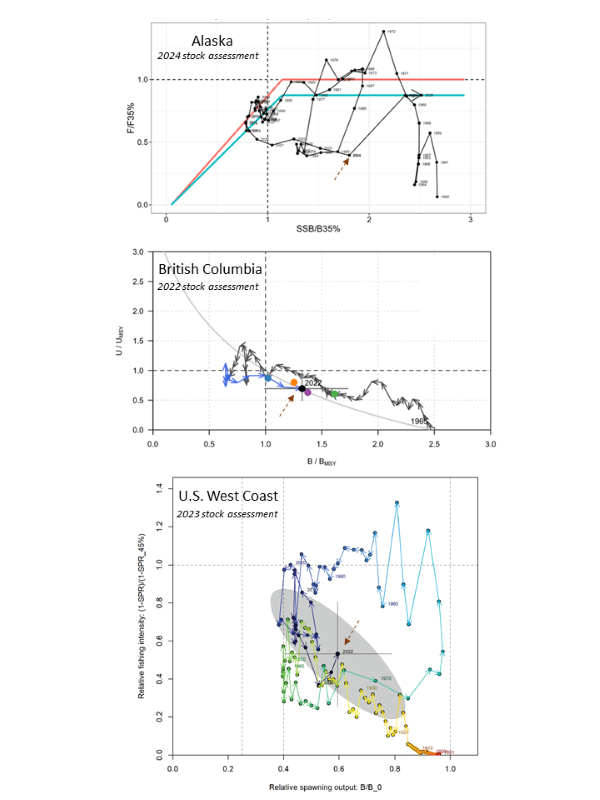
\includegraphics[width=1\linewidth,height=\textheight,keepaspectratio,alt={'The stock in both Alaska and British Columbia is assessed to be above the management target with harvest less that the target harvest rate. The U.S. West Coast stock is assessed to be below the biomass target with harest less than the target harvest rate in 2024.'}]{figures/regional_Kobe.png}

}

\caption{\label{fig-reg-kobe}Time series of sablefish biomass-based and
fishing-based estimates of status in Alaska, British Columbia, and along
the U.S. West Coast from the most recent stock assessments. The arrow
indicates estimates for the current year of the stock assessment.
Vertical and horizontal axes differ by area due to region-dependent
reference point use and specifications.}

\end{figure}%

\subsection{Data}\label{data-2}

\begin{figure}[H]

\centering{

\includegraphics[width=0.95\linewidth,height=\textheight,keepaspectratio,alt={'Line plot with years from 1890-2024 along the x-axis and varying data types used in the assessment along the y-axis. Catch data available from 1890 to 2024 for all fleets. Indices of abundance available starting in 1980 to 2004 and age data from the fishery and surveys available from 1893 to 2024. Age composition data starting in 1983 for the trawl, hook-and-line, and pot fleets.  Age composition data starting in 2006 for the discard fleets. Age composition data from fishery-independent surveys starting in 1983. The WCGBTS survey age composition data were available each year from 2003 through 2024, excluding 2020.'}]{../model/base_model/8.36_base_model/plots/data_plot.png}

}

\caption{\label{fig-data}Data used in the base model.}

\end{figure}%

\newpage

\begin{figure}[H]

\centering{

\includegraphics[width=1\linewidth,height=\textheight,keepaspectratio,alt={'Barplot with year on the x-axis and removals in metric tons on the y-axis. Removals before the 1970s were less than 5,000 mt by year with landings sharply increasing in the 1970s and early 1980s and landings since ranging between approximately 5,000 to 7,500 mt by year.'}]{SAR_USWC_sablefish_skeleton_files/figure-pdf/fig-landings-1.pdf}

}

\caption{\label{fig-landings}Removals in metric tons (mt) by year for
trawl, pot, and hook-and line gears.}

\end{figure}%

\pagebreak

\begin{figure}[H]

\centering{

\includegraphics[width=1\linewidth,height=\textheight,keepaspectratio,alt={'Line plot comparing removals in the 2023 assessment to those used in this assessment with year on the x-axis and total removals in metric tons on the y-axis. The removals between this assessment and the 2023 assessment are nearly equal for all years in the model.'}]{SAR_USWC_sablefish_skeleton_files/figure-pdf/fig-landings-comparison-1.pdf}

}

\caption{\label{fig-landings-comparison}Comparison of the total removals
in metric tons (mt) by year between this assessment and the 2023
assessment.}

\end{figure}%

\pagebreak

\begin{figure}[H]

\centering{

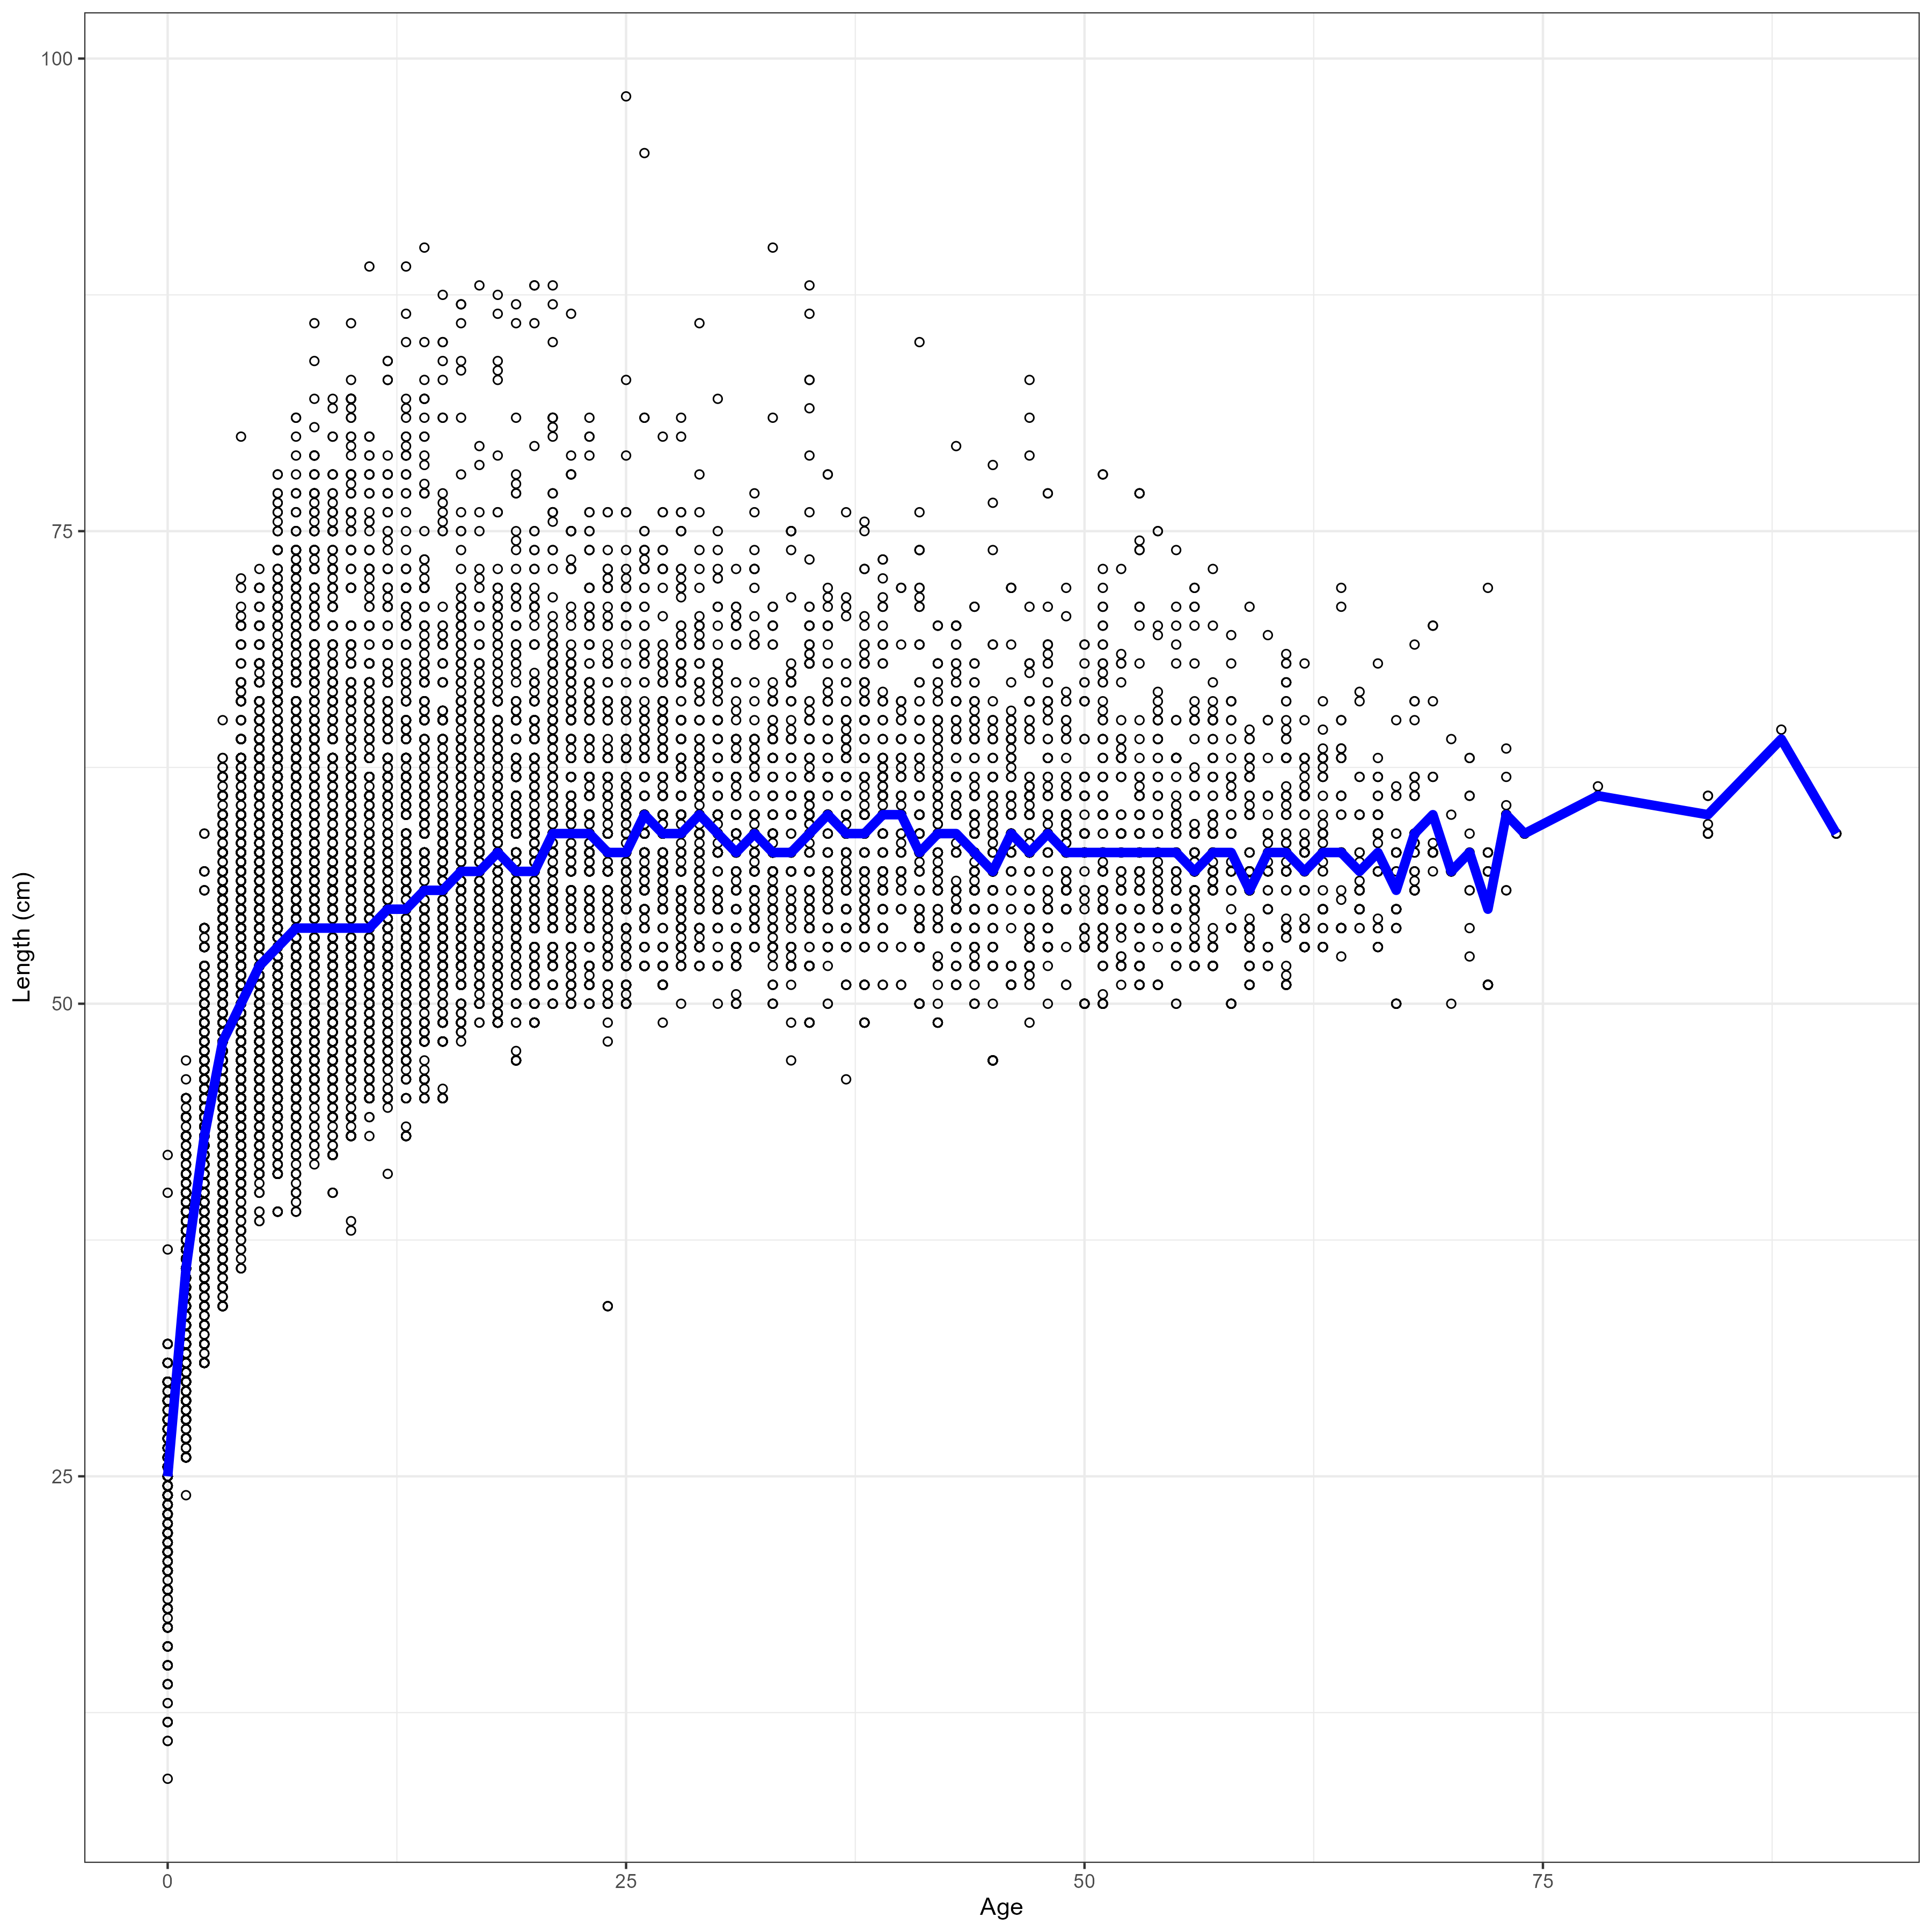
\includegraphics[width=1\linewidth,height=\textheight,keepaspectratio,alt={'Data point plot with estimated age on the x-axis and length in centimeters on the y-axis with three panels showing the data from the trawl discard, hook-and-line discard, and pot discard fleets. The estimated age from length for each gear approximate the expected length-age growth curve for sablefish.'}]{figures/compare_data_alk_all_years.png}

}

\caption{\label{fig-alk}Comparison of estimated discard age by length
for each gear type.}

\end{figure}%

\begin{figure}[H]

\centering{

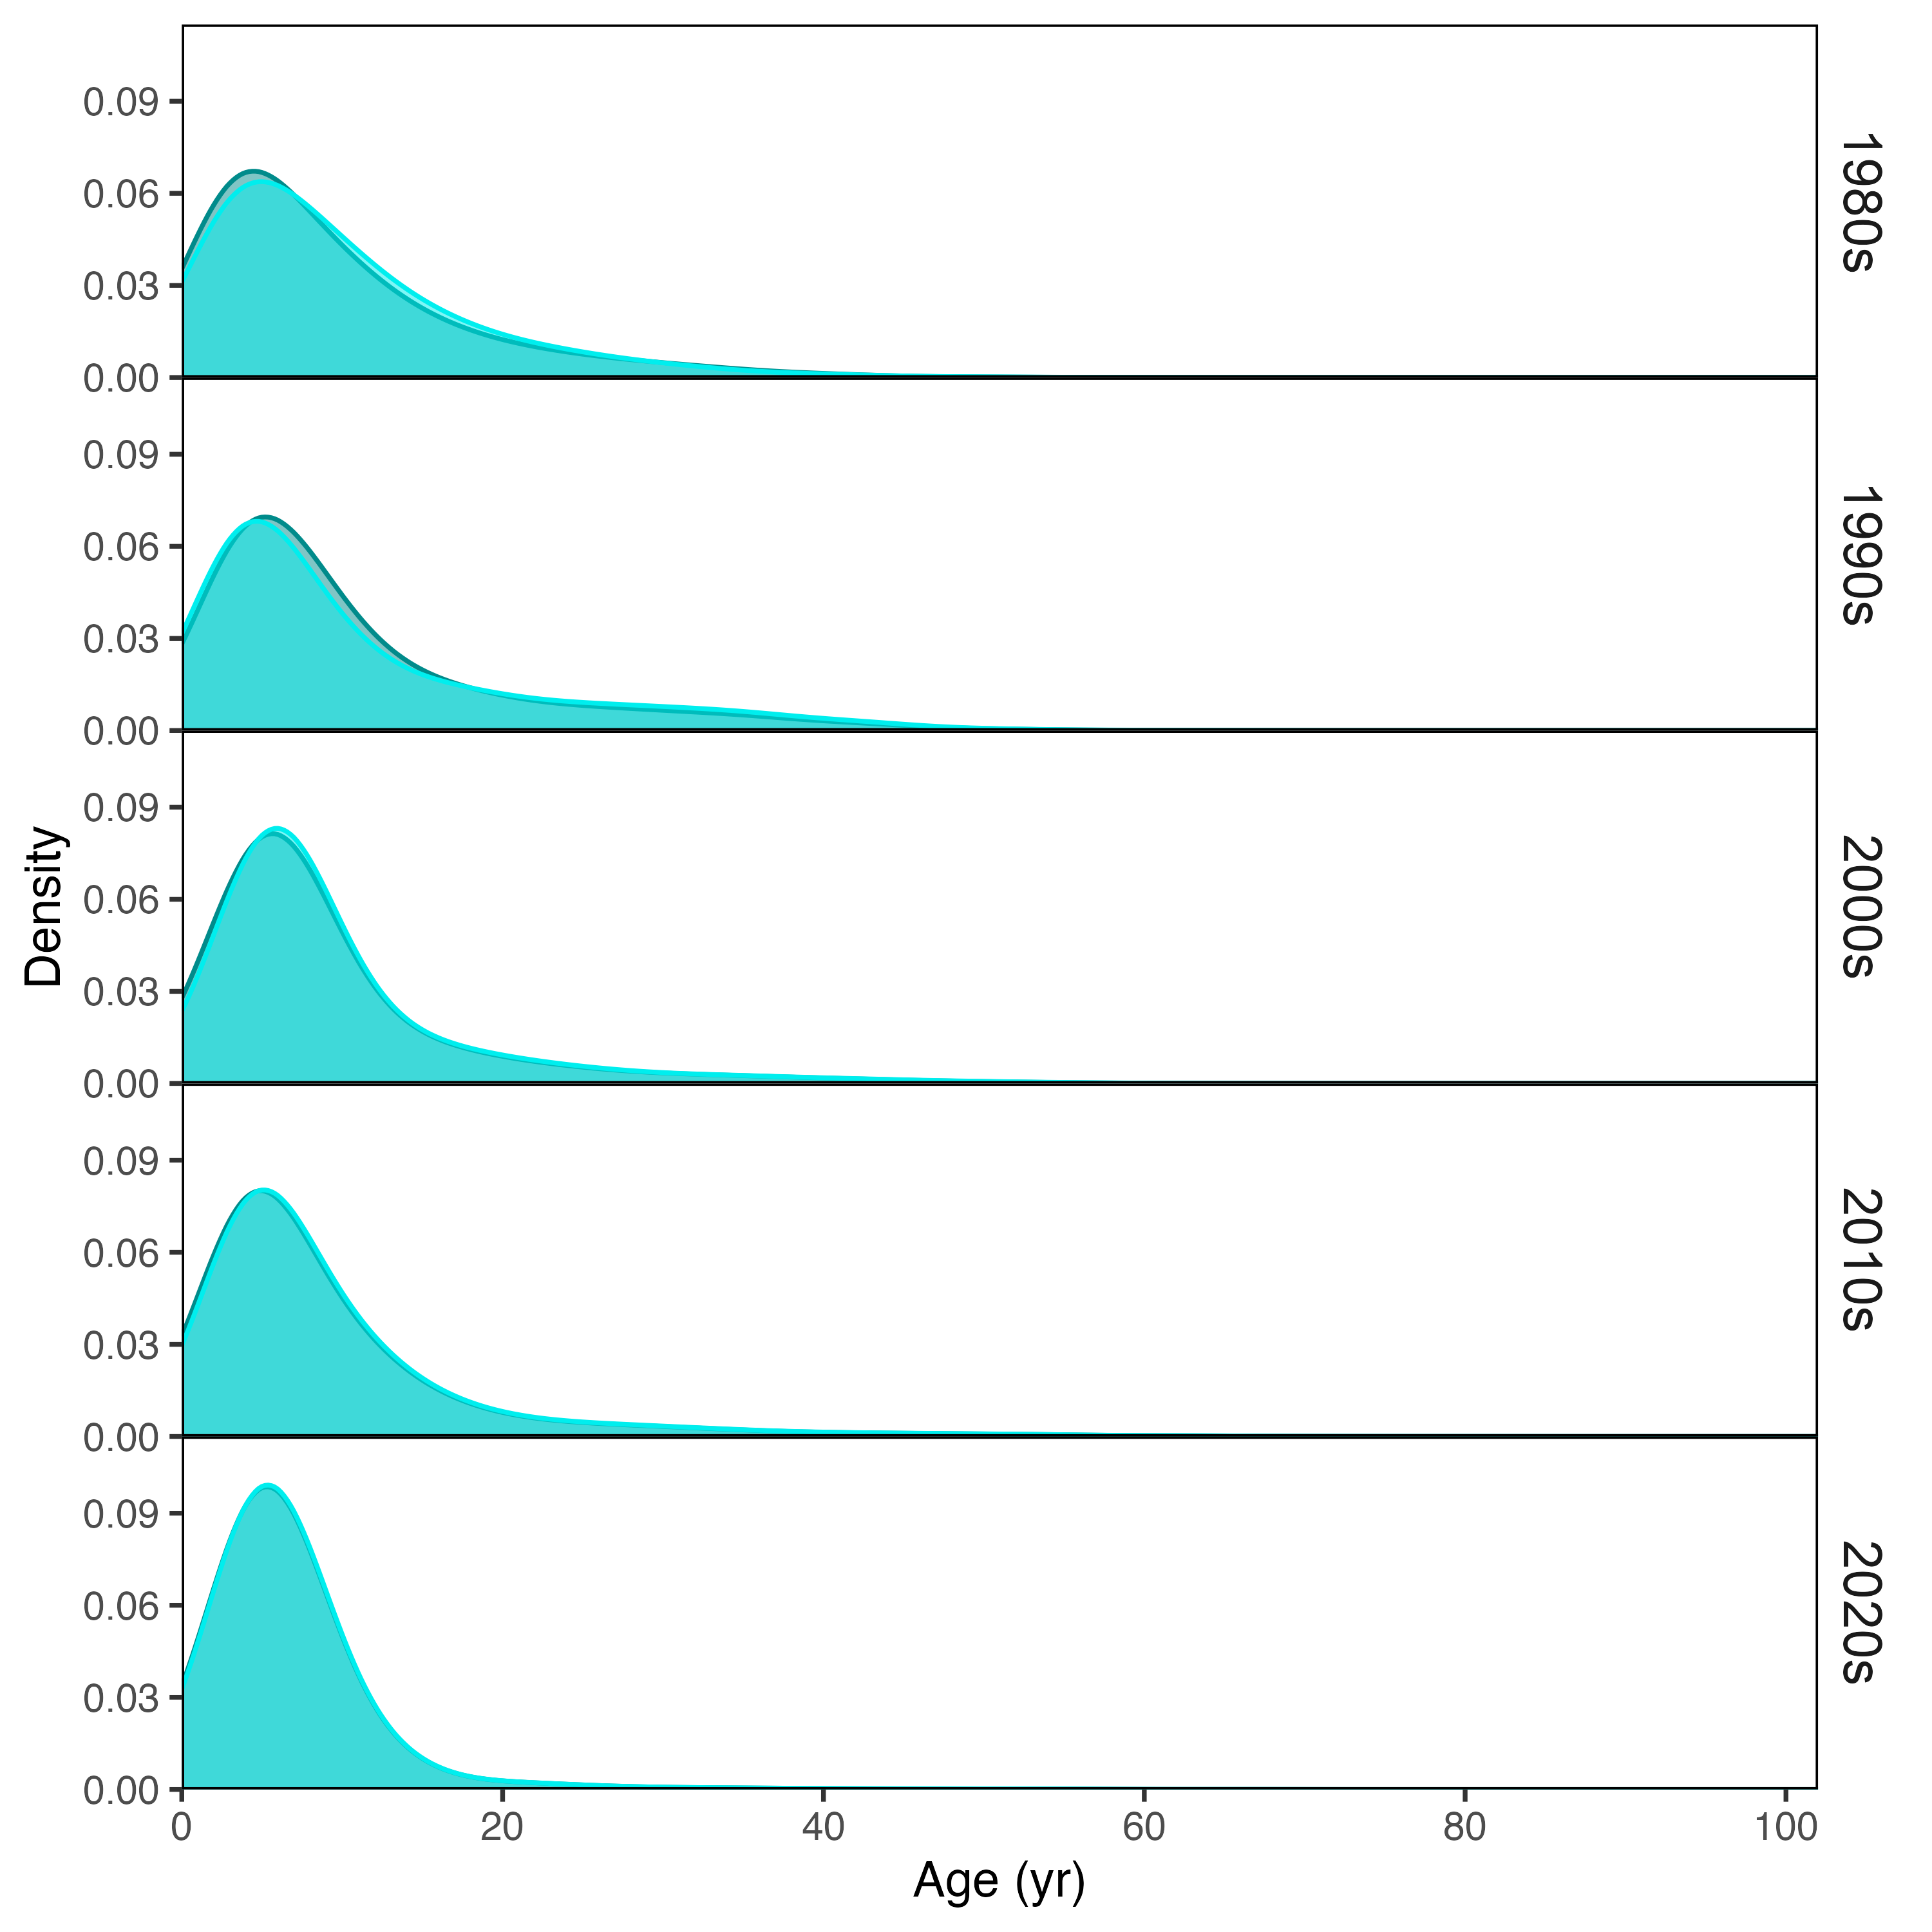
\includegraphics[width=1\linewidth,height=\textheight,keepaspectratio,alt={'Density plot with age in years on the x-axis with panels for each decade of data. The density of samples by age grouped by decade 1980s, 1990s, 2000s, 2010s, and 2020s are nearly identical for the ages used in the 2019 assessment and the additional ages included in this assessment.'}]{figures/age_dist_decade.png}

}

\caption{\label{fig-age-comp}Distribution of ages before (dark color)
and after (light color) removing samples without an ageing method
assigned and those collected as part of special projects by decade.}

\end{figure}%

\begin{figure}[H]

\centering{

\includegraphics[width=1\linewidth,height=\textheight,keepaspectratio,alt={'Line plot with age in years on the x-axis and proportion on the y-axis with separate panels for each fleet in the model with age data. The distribution of ages for the trawl gear peak around age 5 for both males and females. The hook-and-line and pot gear select more females compared to males with the distribution of ages peak at slightly older ages compare to the trawl fleet. Trawl discard ages are primarily young fish between age 0 to 4 with hook-and-line and pot discarding slightly older ages compared to trawl. '}]{../model/base_model/8.36_base_model/plots/comp_agedat__aggregated_across_time.png}

}

\caption{\label{fig-data-agg-ages}Aggregated ages across all years by
fleet.}

\end{figure}%

\begin{figure}[H]

\centering{

\includegraphics[width=1\linewidth,height=\textheight,keepaspectratio,alt={'Plot with year on the x-axis and age in years on the y-axis with open circles indicating the proportion of samples at each age for each year with data. The majority of ages discarded by the trawl discard fleet are less than 3 years of age with limited discarding of older fish.'}]{../model/base_model/8.36_base_model/plots/comp_agedat_bubflt4mkt0.png}

}

\caption{\label{fig-discard-ages-trawl}Ages by year for the trawl
discard fleet. All ages are unsexed.}

\end{figure}%

\begin{figure}[H]

\centering{

\includegraphics[width=1\linewidth,height=\textheight,keepaspectratio,alt={'Plot with year on the x-axis and age in years on the y-axis with open circles indicating the proportion of samples at each age for each year with data. The majority of ages discarded by the hook-and-line discard fleet are less than 5 years of age with some limited discarding of older fish.'}]{../model/base_model/8.36_base_model/plots/comp_agedat_bubflt5mkt0.png}

}

\caption{\label{fig-discard-ages-hkl}Ages by year for the hook-and-line
discard fleet. All ages are unsexed.}

\end{figure}%

\begin{figure}[H]

\centering{

\includegraphics[width=1\linewidth,height=\textheight,keepaspectratio,alt={'Plot with year on the x-axis and age in years on the y-axis with open circles indicating the proportion of samples at each age for each year with data. The majority of ages discarded by the pot discard fleet are less than 5 years of age with appreciable discarding of older fish.'}]{../model/base_model/8.36_base_model/plots/comp_agedat_bubflt6mkt0.png}

}

\caption{\label{fig-discard-ages-pot}Ages by year for the pot discard
fleet. All ages are unsexed.}

\end{figure}%

\pagebreak

\begin{figure}[H]

\centering{

\includegraphics[width=1\linewidth,height=\textheight,keepaspectratio,alt={'Plot with year on the x-axis and age in years on the y-axis with open circles indicating the proportion of samples by sex at each age for each year with data. The trawl fleet ages show similar proportions between females and males with clear evidence of strong recruitments moving through the fishery.'}]{../model/base_model/8.36_base_model/plots/comp_agedat_bubflt1mkt0_page2.png}

}

\caption{\label{fig-data-trawl}Age composition by year and sex for the
trawl fleet. Females are shown in red, males in blue, and unsexed fish
in grey.}

\end{figure}%

\pagebreak

\begin{figure}[H]

\centering{

\includegraphics[width=1\linewidth,height=\textheight,keepaspectratio,alt={'Plot with year on the x-axis and age in years on the y-axis with open circles indicating the proportion of samples by sex at each age for each year with data. The hook-and-line fleet ages show greater proportions of females than males with clear evidence of strong recruitments moving through the fishery. The largest frequency of ages occur of fish between 3 to 10 years of age.'}]{../model/base_model/8.36_base_model/plots/comp_agedat_bubflt2mkt0_page2.png}

}

\caption{\label{fig-data-hkl}Age composition by year and sex for the
hook-and-line fleet. Females are shown in red and males in blue.}

\end{figure}%

\pagebreak

\begin{figure}[H]

\centering{

\includegraphics[width=1\linewidth,height=\textheight,keepaspectratio,alt={'Plot with year on the x-axis and age in years on the y-axis with open circles indicating the proportion of samples by sex at each age for each year with data. The pot fleet ages show greater proportions of females than males with clear evidence of strong recruitments moving through the fishery. The largest frequency of ages occur of fish between 4 to 10 years of age.'}]{../model/base_model/8.36_base_model/plots/comp_agedat_bubflt3mkt0_page2.png}

}

\caption{\label{fig-data-pot}Age composition by year and sex for the pot
fleet. Females are shown in red and males in blue.}

\end{figure}%

\pagebreak

\begin{figure}[H]

\centering{

\includegraphics[width=1\linewidth,height=\textheight,keepaspectratio,alt={'Line plot with year on the x-axis and standardize index values on the y-axis.  Each index is standardized to the mean of the index. The standardized indices shows the population potentially decreasing between 1980 and 2010. Slowly increasing from 2011 to 2019 and sharply increasing at the end of the time series.'}]{../model/base_model/8.36_base_model/plots/index9_standcpueall.png}

}

\caption{\label{fig-index-stand}Relative indices of abundance used in
the base model standardized and overlaid. Each index is rescaled to have
mean observation = 1.0.}

\end{figure}%

\pagebreak

\begin{figure}[H]

\centering{

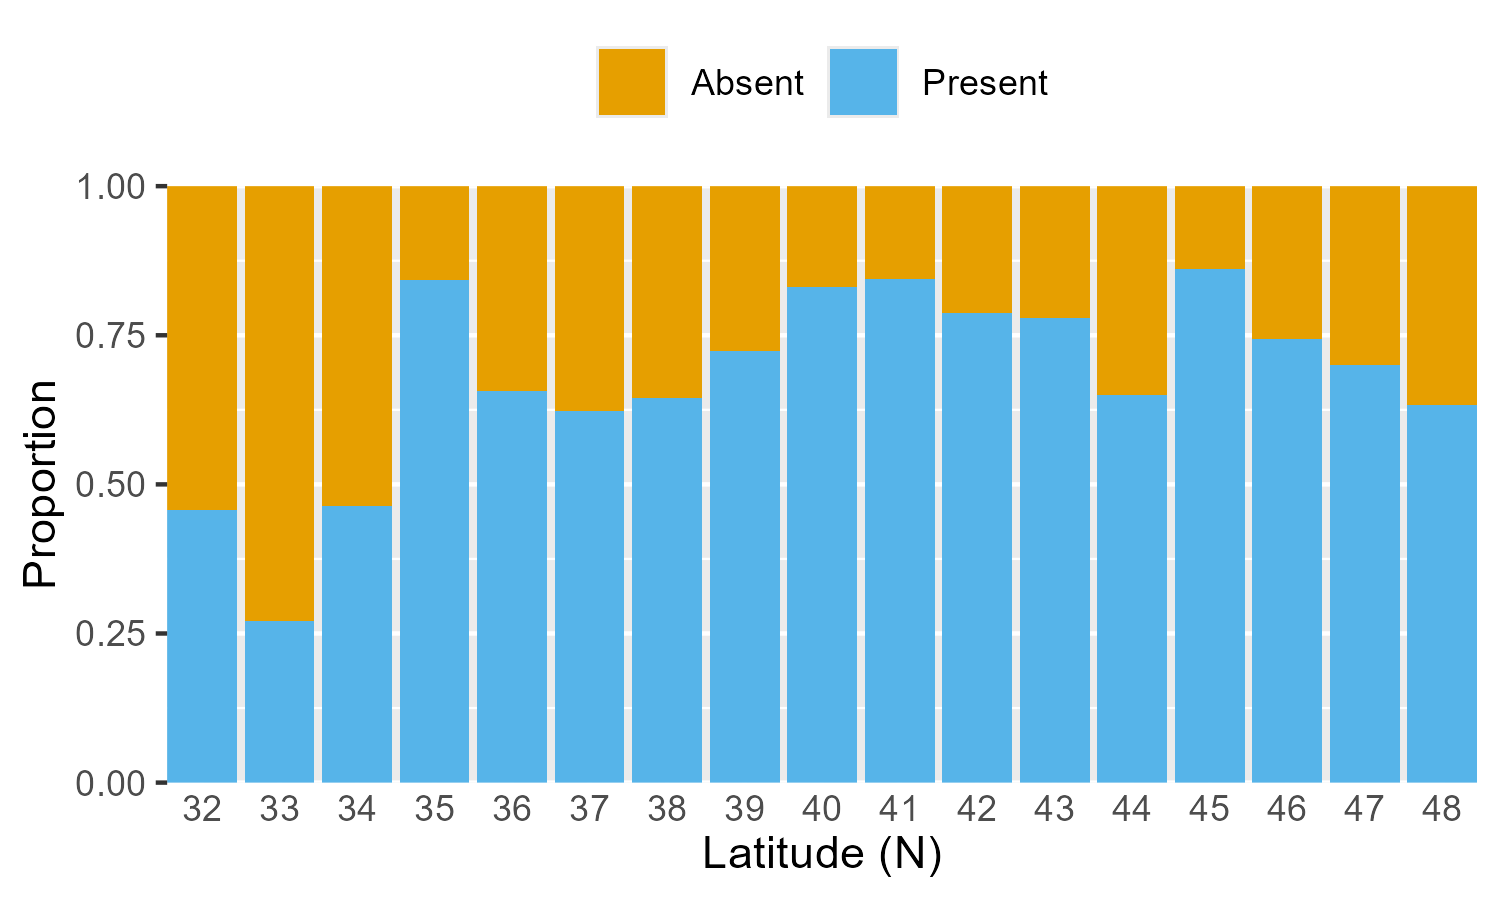
\includegraphics[width=1\linewidth,height=\textheight,keepaspectratio,alt={'Barplot with latitude on the x-axis and proportion on the y-axis. The proportion of postive tows is approximately 75 percent of all tows north of Point Conception with a lower proportion positive south of Point Conception between 25 to 45 percent.'}]{figures/wcgbts_present_absense.png}

}

\caption{\label{fig-positive-lat-wcgbt}Proportion of tows where
sablefish was present or absent across all years by latitude for the
NWFSC West Coast Groundfish Bottom Trawl Survey.}

\end{figure}%

\begin{figure}[H]

\centering{

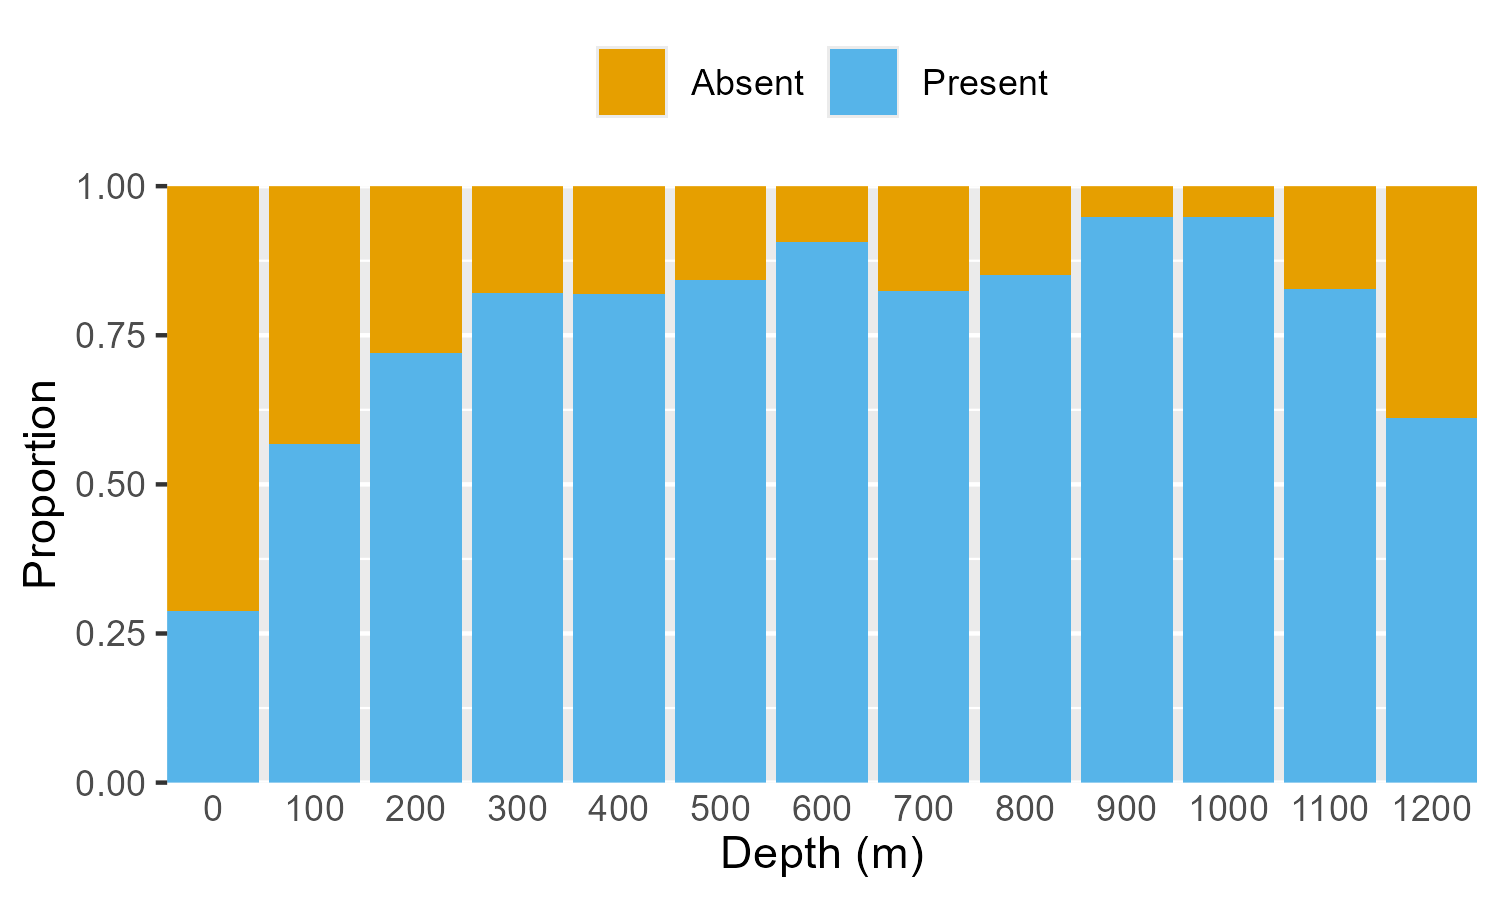
\includegraphics[width=1\linewidth,height=\textheight,keepaspectratio,alt={'Barplot with depth along the x-axis and proportion along the y-axis. The data by depth are shown in 100 meter bins starting at 0-100 meters up through 1,200-1,300 meters. The frequency of observed tows increases from 25 percent for depths less than 100 meters to roughly 75 percent across depths from 300 to 1200 meters and a decrease to 60 percent for the greatest depths sampled.'}]{figures/wcgbts_present_absense_depth.png}

}

\caption{\label{fig-positive-depth-wcgbt}Proportion of tows where
sablefish was present or absent across all years by depth (m) for the
NWFSC West Coast Groundfish Bottom Trawl Survey.}

\end{figure}%

\pagebreak

\begin{figure}[H]

\centering{

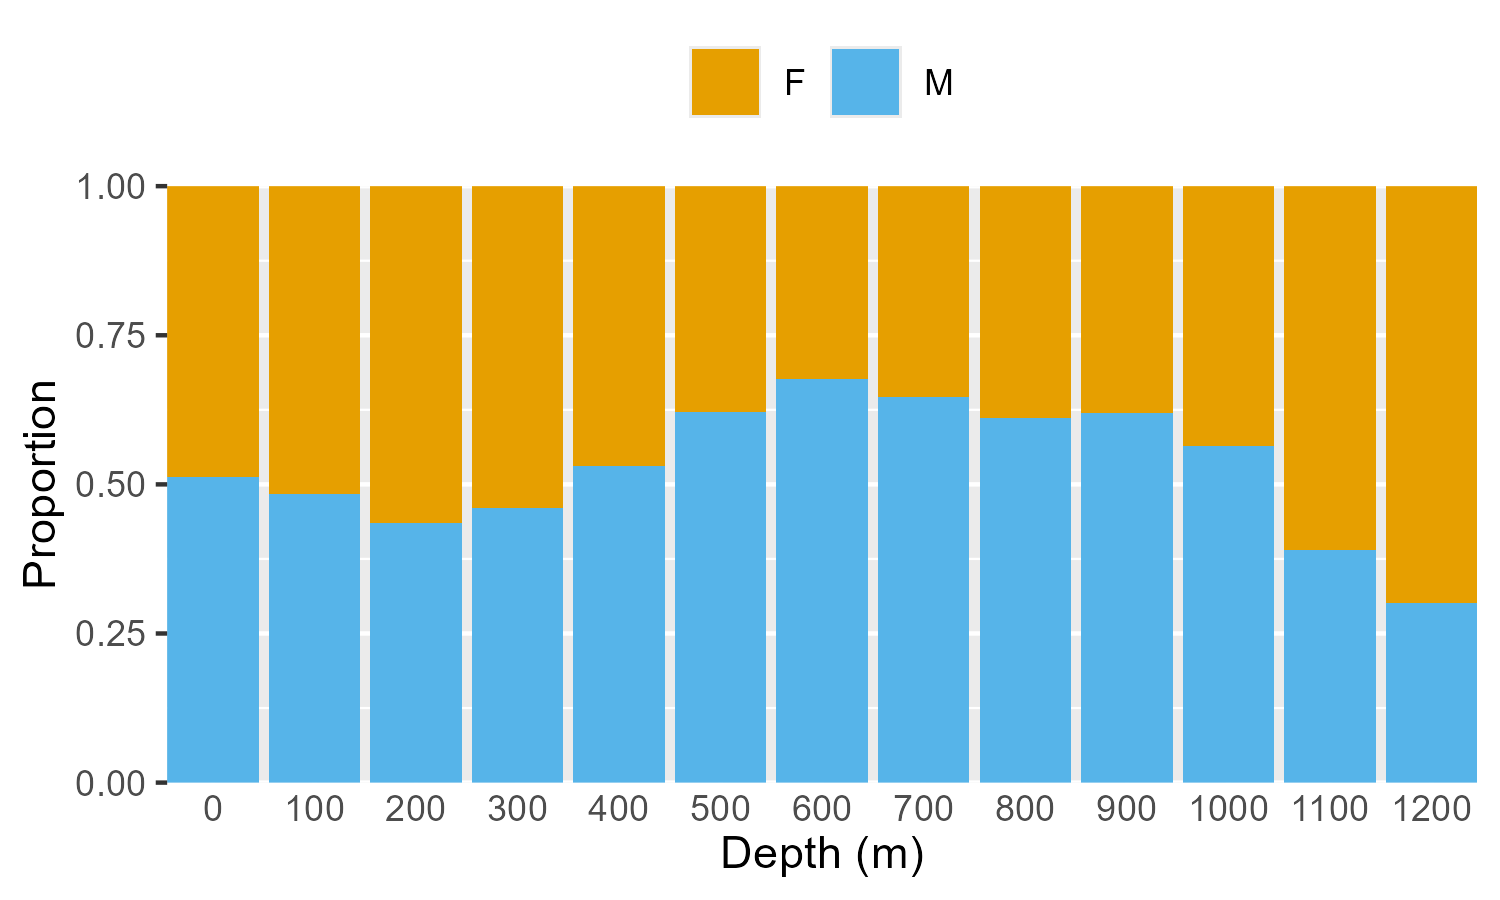
\includegraphics[width=1\linewidth,height=\textheight,keepaspectratio,alt={'Barplot with depth along the x-axis and proportion along the y-axis. The data by depth are shown in 100 meter bins starting at 0-100 meters up through 1,200-1,300 meters. The sex ratio is approximately 50-50 out to 500 meters and the propotion of females declines to less than 50 percent out to 1100 meters and then increases to greater than 50 percent at the greatest depths sampled.'}]{figures/wcgbts_sex_ratio_depth.png}

}

\caption{\label{fig-sex-ratio-wcgbt}Sex ratio across all years by depth
(m) for the NWFSC West Coast Groundfish Bottom Trawl Survey.}

\end{figure}%

\pagebreak

\begin{figure}[H]

\centering{

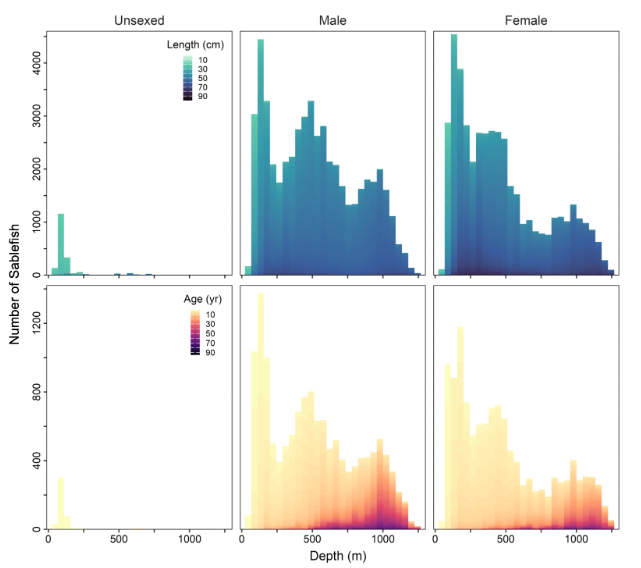
\includegraphics[width=1\linewidth,height=\textheight,keepaspectratio,alt={'Barplot with depth in meters along the x-axis and numbers along the y-axis with separate panels by sex.  The top row shows the numbers by lengths by depth and sex and the bottom row shows the number of ages by depth and sex. Older and larger sablefish for all sexes are found in greater frequency at deeper depths with waters greater than 500 meters have the greatest proportion of the oldest sablefish.'}]{figures/wcgbts_length_age_compositions.png}

}

\caption{\label{fig-wcgbt-depth-len-age}Length (top; cm) and age
(bottom; yr) compositions for sablefish collected by the NWFSC West
Coast Groundfish Bottom Trawl Survey between 2003 and 2024 by sex and
depth (m). Lighter colors represent smaller or younger individuals and
darker colors represent larger or older individuals.}

\end{figure}%

\pagebreak

\begin{figure}[H]

\centering{

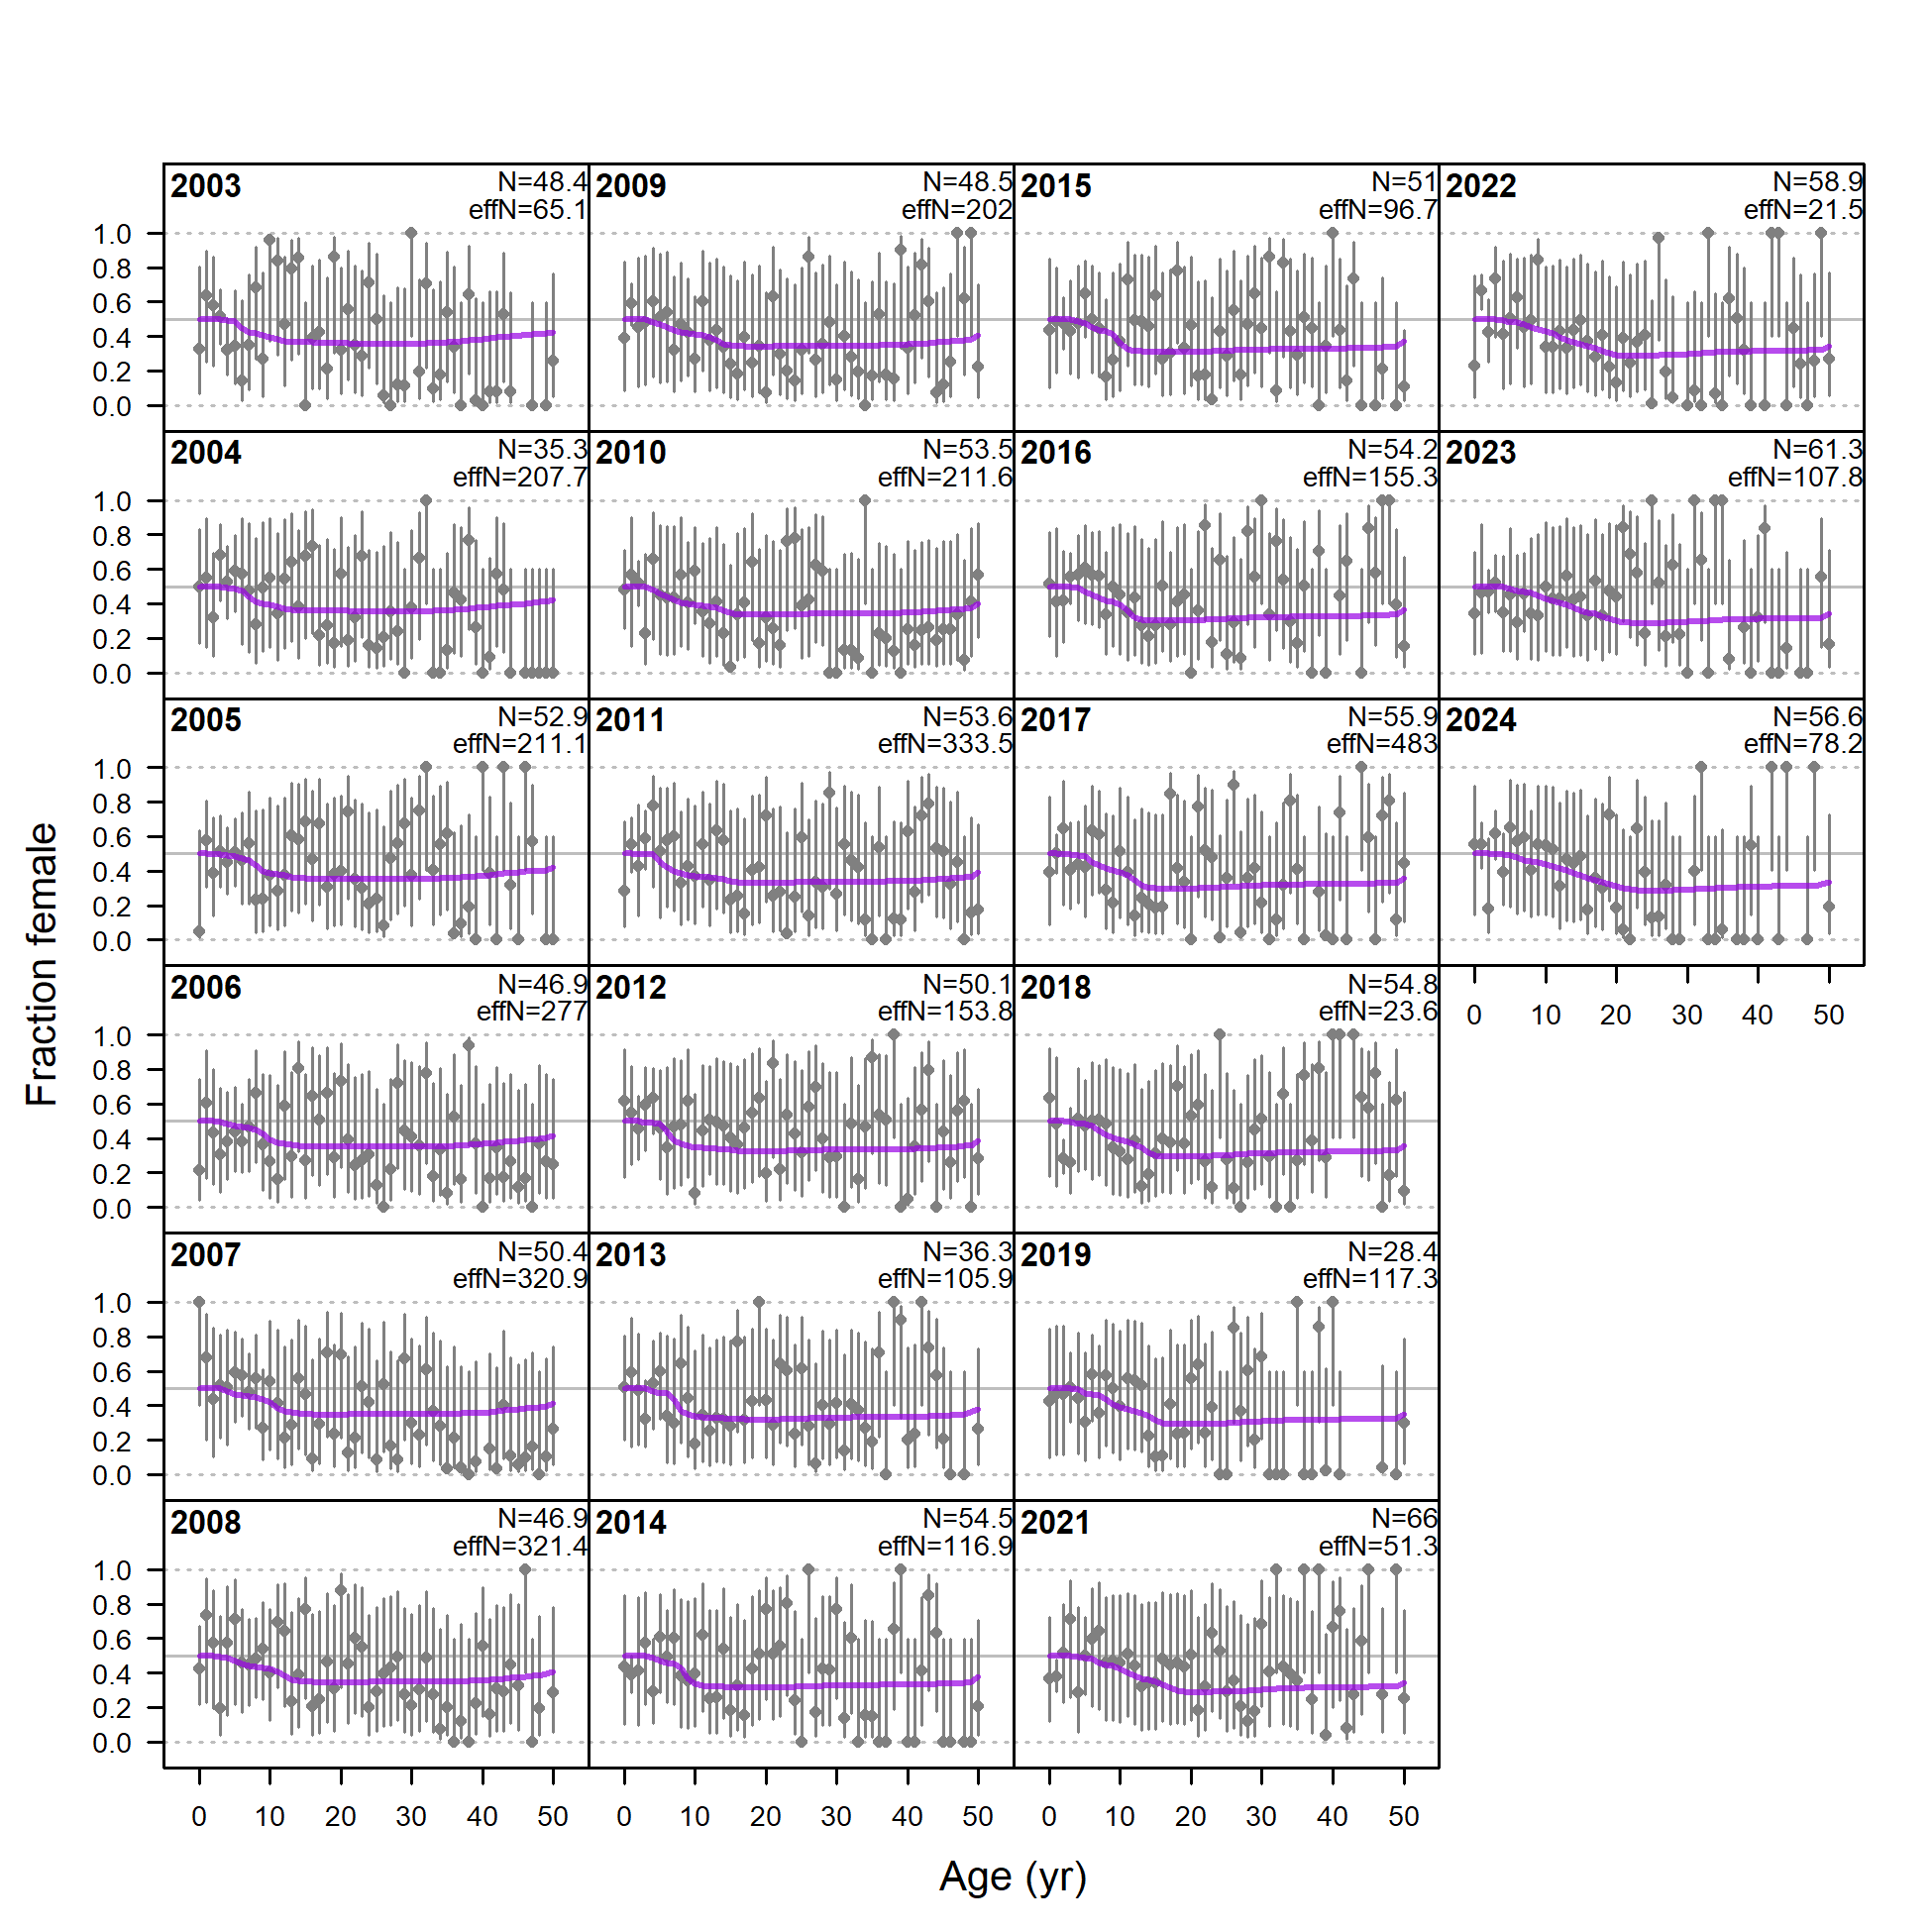
\includegraphics[width=1\linewidth,height=\textheight,keepaspectratio,alt={'Line plot with age in years along the x-axis and the fraction female along the y-axis with separate panels for data by year from the WCGBTS. The fraction of female sablefish is roughly 0.50 at age 0 with the fraction of female fish decreasing to less than 0.40 for ages 10 and older for each year in the WCGBTS survey data from 2003 through 2024.'}]{figures/sexratio_age_flt10mkt0.png}

}

\caption{\label{fig-wcgbt-age-sex-ratio}Observed fraction female by age
in the NWFSC West Coast Groundfish Bottom Trawl Survey by year.}

\end{figure}%

\pagebreak

\begin{figure}[H]

\centering{

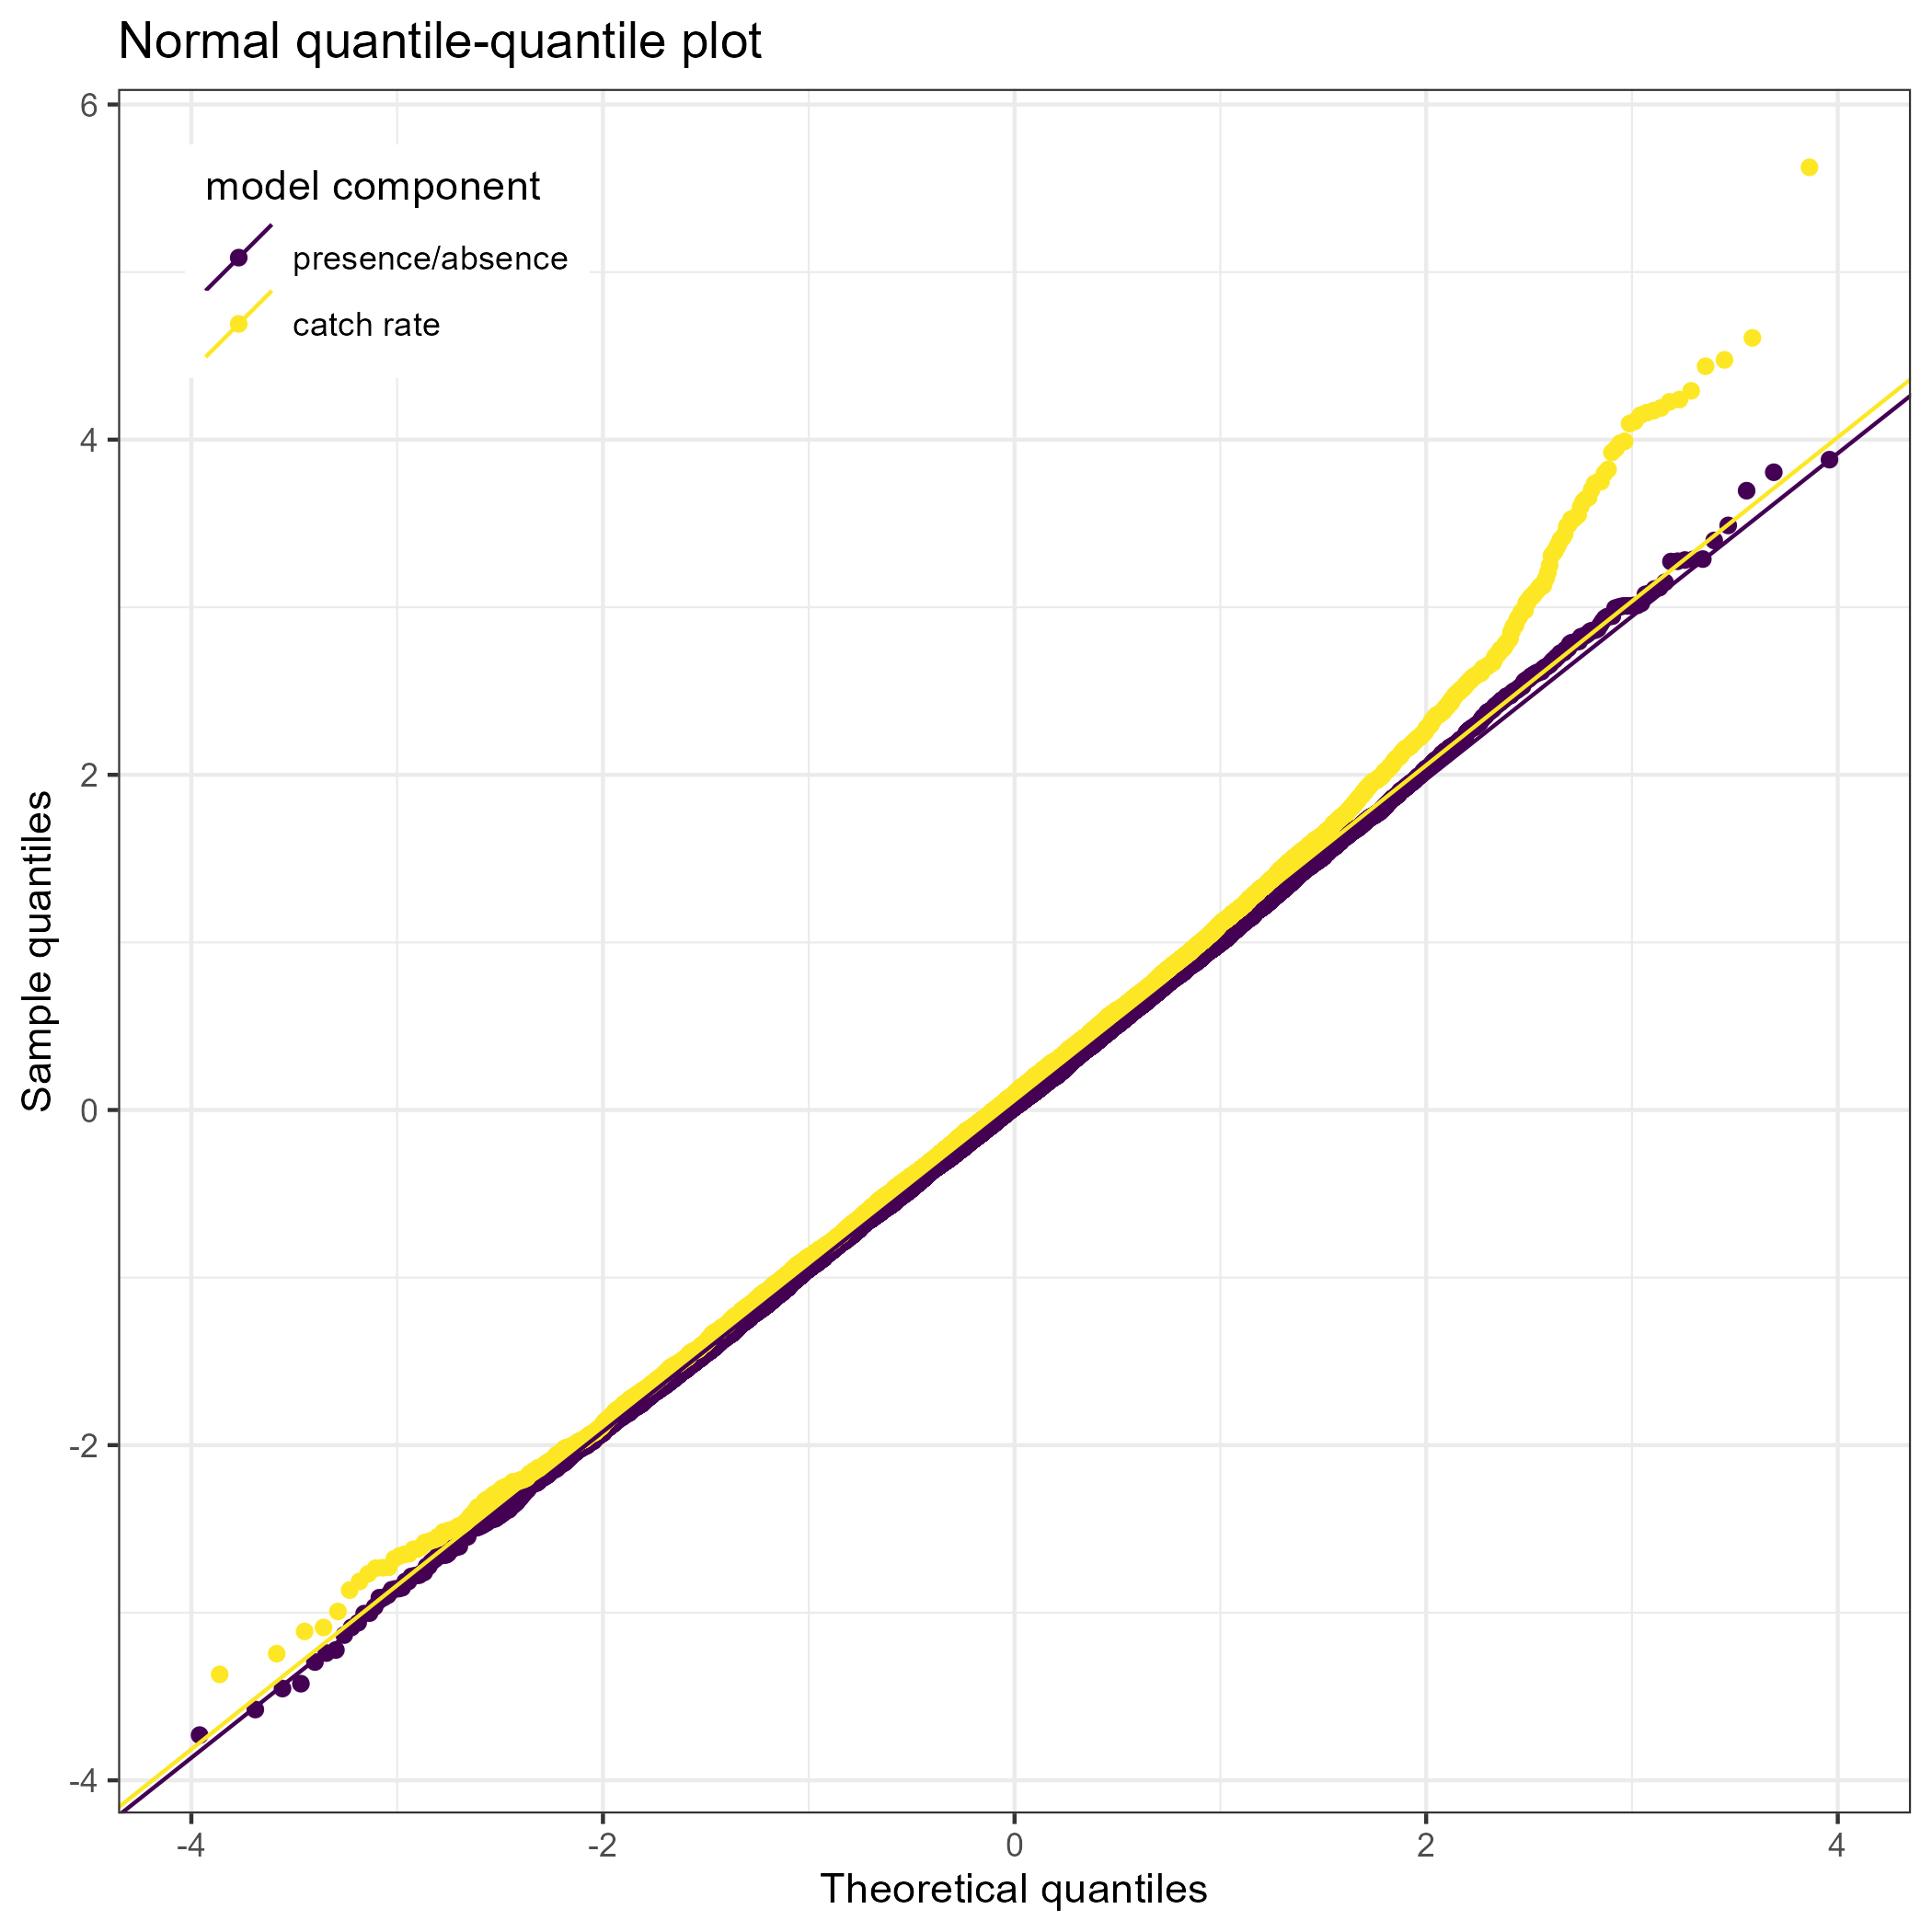
\includegraphics[width=1\linewidth,height=\textheight,keepaspectratio,alt={'Line plot with the theoretical quantiles along the x-axis and sample quantiles along the y-axis. The plot has a one-to-one line, points for the catch rate model, and points for the presence/absence model. The sample and theoretical quantiles for the presence/absence and catch rate models are roughly one to one with some departure at the larger quantiles for the catch rate model. '}]{figures/wcgbt_qq.png}

}

\caption{\label{fig-qq-wcgbt}QQ plot for the NWFSC West Coast Groundfish
Bottom Trawl Survey.}

\end{figure}%

\pagebreak

\begin{figure}[H]

\centering{

\includegraphics[width=1\linewidth,height=\textheight,keepaspectratio,alt={'Line plot with year along the x-axis and relative abundance in metric tons along the y-axis with point and uncertainty intervals show for each year. The index decreases from 2003 to 2010 and then slowly increases until 2018 declines for 2019 and then sharply increases in 2021 and 2022 and is roughly stable in the final years.'}]{../model/base_model/8.36_base_model/plots/index1_cpuedata_WCGBTS.png}

}

\caption{\label{fig-index-wcgbt}Relative index of abundance for the
NWFSC West Coast Groundfish Bottom Trawl Survey.}

\end{figure}%

\pagebreak

\begin{figure}[H]

\centering{

\includegraphics[width=1\linewidth,height=\textheight,keepaspectratio,alt={'Plot with year on the x-axis and age in years on the y-axis with open circles indicating the proportion of samples by sex at each age for each year with data. The proportion of observations by year, age, and sex has larger proportions at younger ages with evidence of potential year classes moving through the population.'}]{../model/base_model/8.36_base_model/plots/comp_agedat_bubflt10mkt0.png}

}

\caption{\label{fig-data-wcgbt}Age composition data by year from the
NWFSC West Coast Groundfish Bottom Trawl Survey. Females are shown in
red, males in blue, and unsexed fish in grey.}

\end{figure}%

\begin{figure}[H]

\centering{

\includegraphics[width=1\linewidth,height=\textheight,keepaspectratio,alt={'Line plot with year along the x-axis and mean age along the y-axis with median values and quantiles shown for each year of data. The mean age for sexed fish increased from 2003 through 2008 dropped and was roughly stable from 2009 through 2013 and dropped in 2019 and has been lower in recent years likely due to strong year classes with an increased frequency of young sablefish in the population.'}]{../model/base_model/8.36_base_model/plots/comp_agedat_data_weighting_TA1-8_WCGBTS.png}

}

\caption{\label{fig-data-wcgbt-mean-age}Mean age for NWFSC West Coast
Groundfish Bottom Trawl Survey with 95 percent confidence intervals
based on current sample sizes. The top panel is sexed ages only and the
bottom panel includes both sexed and unsexed ages.}

\end{figure}%

\begin{figure}[H]

\centering{

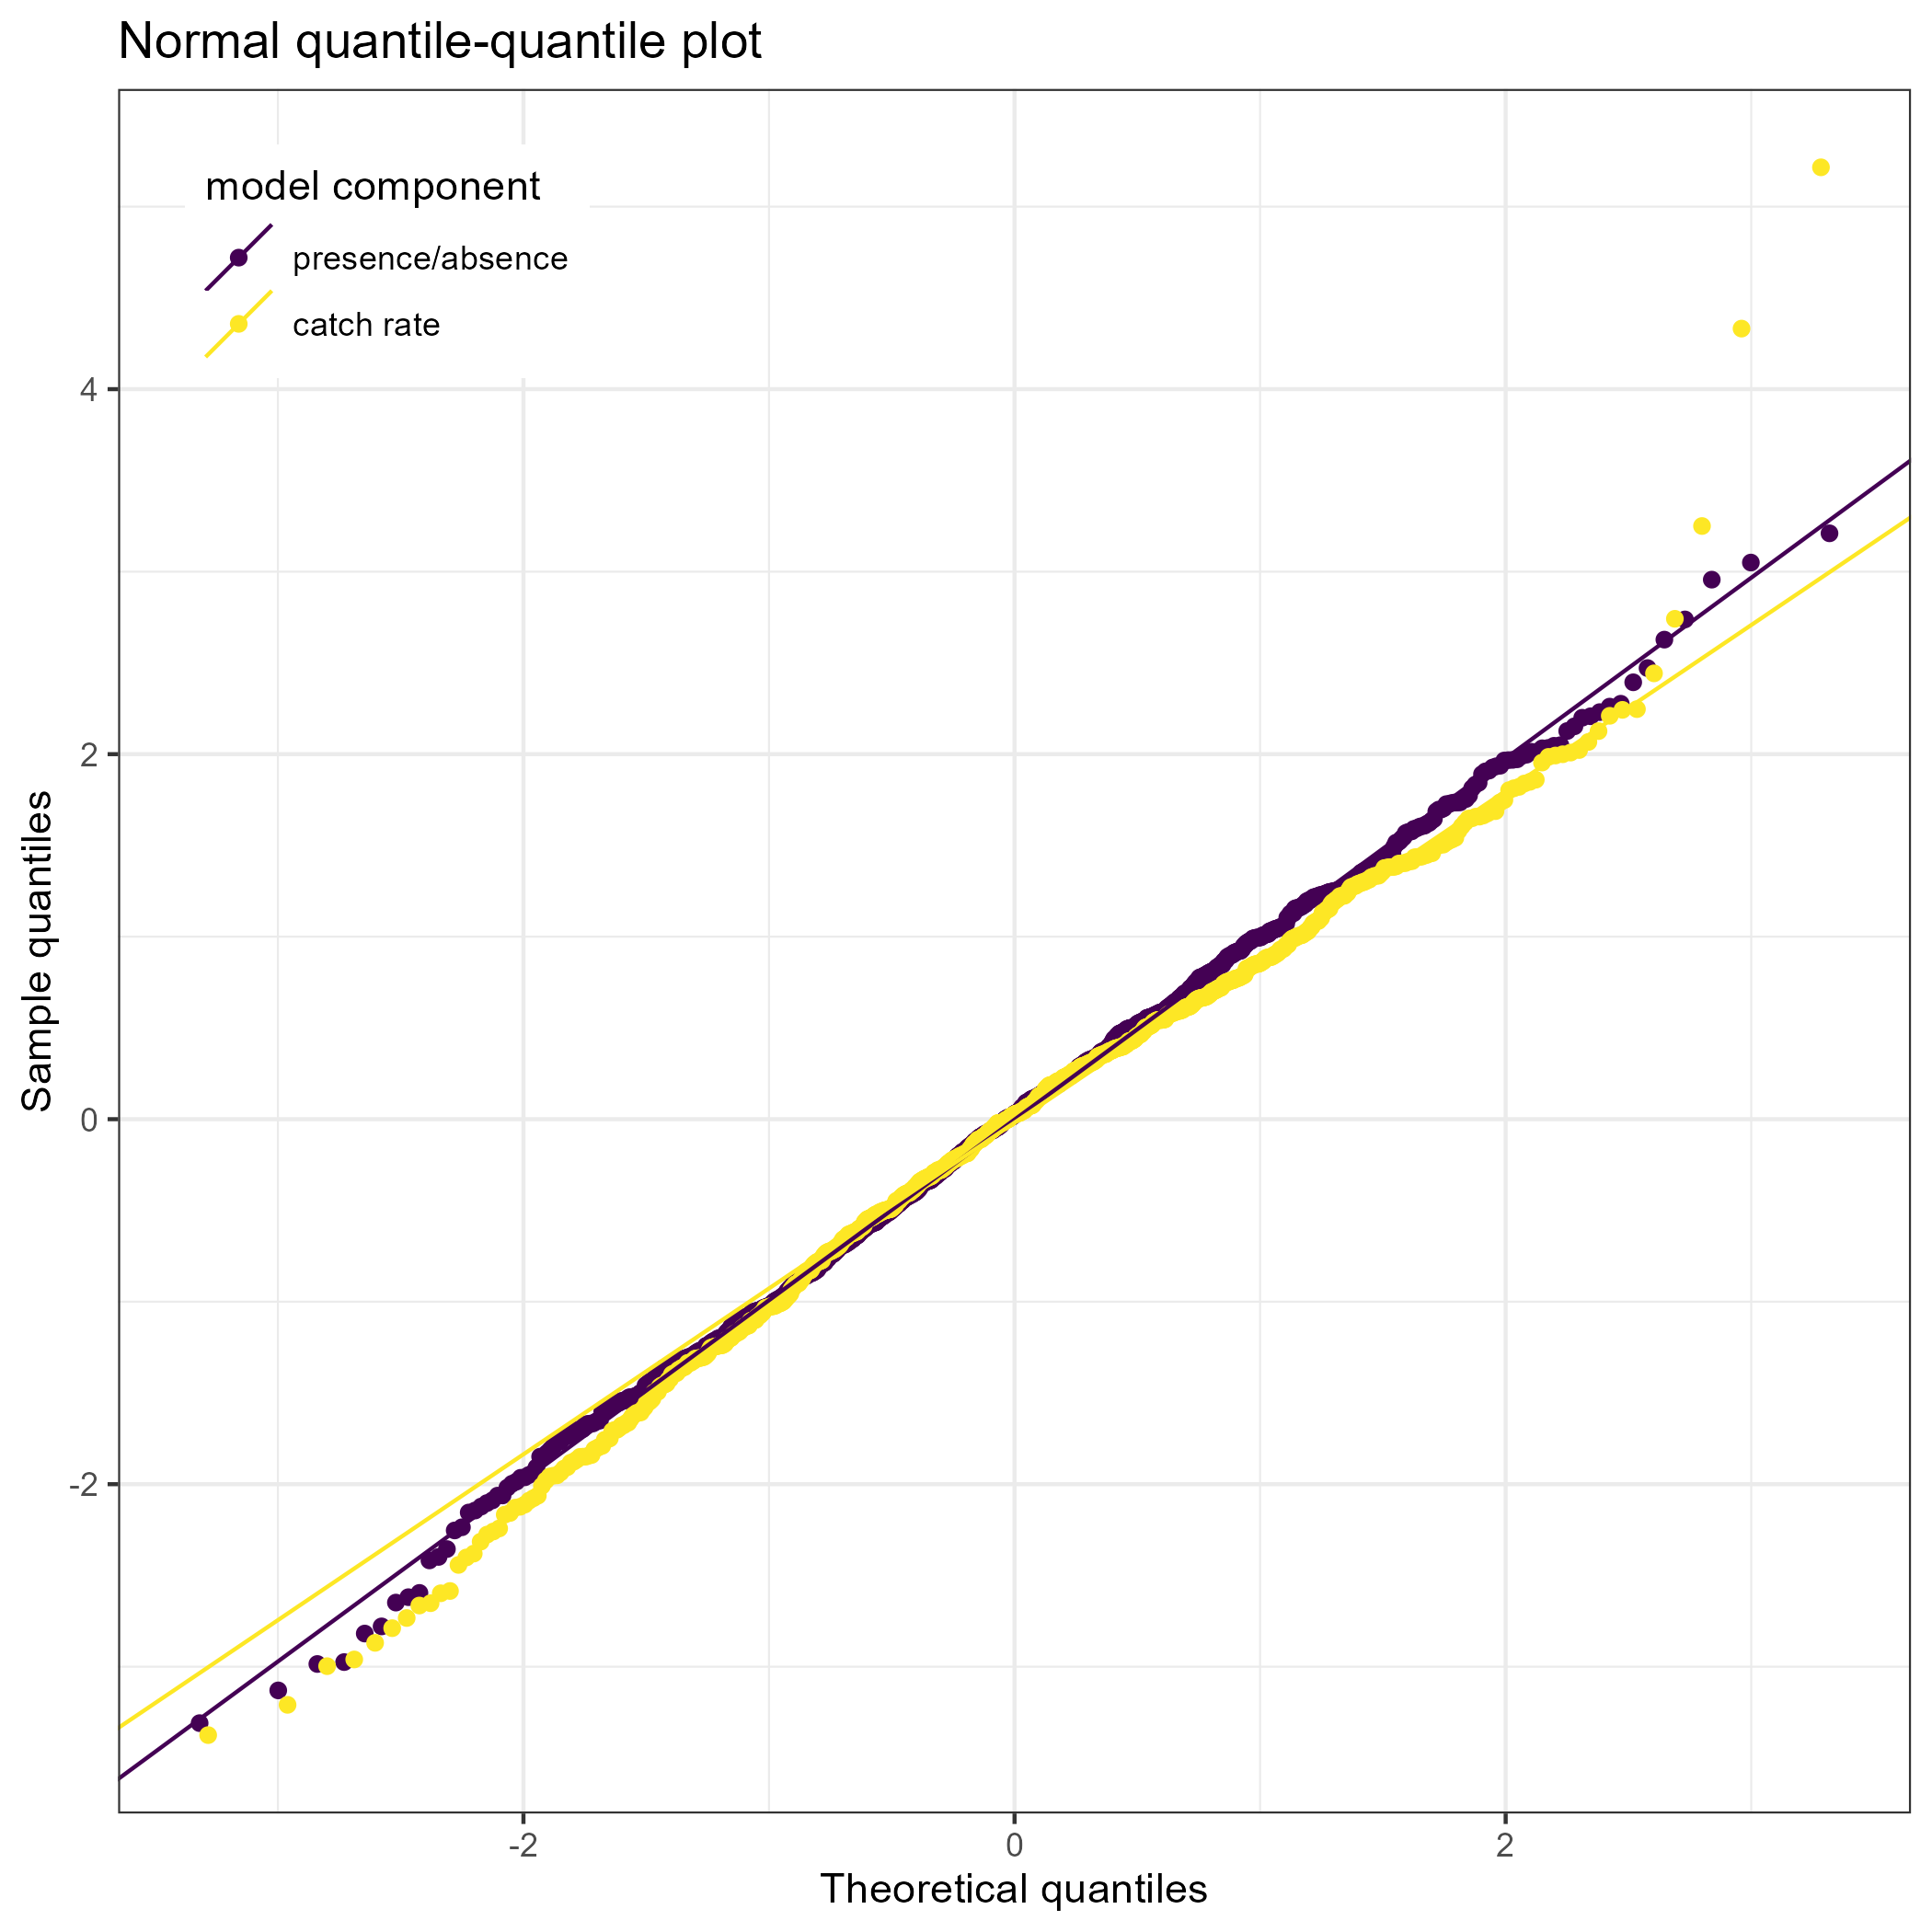
\includegraphics[width=1\linewidth,height=\textheight,keepaspectratio,alt={'Line plot with the theoretical quantiles along the x-axis and sample quantiles along the y-axis. The plot has a one-to-one line, points for the catch rate model, and points for the presence/absence model. The sample and theoretical quantiles for the presence/absence and catch rate models are roughly one to one with some departure at the larger quantiles for the catch rate model.'}]{figures/nwfsc_slope_qq.png}

}

\caption{\label{fig-qq-nwfslope}QQ plot for the NWFSC Slope Survey.}

\end{figure}%

\pagebreak

\begin{figure}[H]

\centering{

\includegraphics[width=1\linewidth,height=\textheight,keepaspectratio,alt={'Line plot with year along the x-axis and relative abundance in metric tons along the y-axis with point and uncertainty intervals show for each year. The trend in the index slightly increases from 1998, 1999, and 2000, decreases slightly in 2001, and then increases in 2002.'}]{../model/base_model/8.36_base_model/plots/index1_cpuedata_NWFSC_Slope.png}

}

\caption{\label{fig-index-nwslope}Relative index of abundance for the
NWFSC Slope Survey.}

\end{figure}%

\pagebreak

\begin{figure}[H]

\centering{

\includegraphics[width=1\linewidth,height=\textheight,keepaspectratio,alt={'Plot with year on the x-axis and age in years on the y-axis with open circles indicating the proportion of samples by sex at each age for each year with data. The proportion of ages by year, age, and sex with the survey observing all ages except for little to no observations of age 0 and 1 fish.'}]{../model/base_model/8.36_base_model/plots/comp_agedat_bubflt9mkt0.png}

}

\caption{\label{fig-data-nwfsc-slope}Age compositions by year from the
NWFSC Slope Survey. Females are shown in red, males in blue, and unsexed
fish in grey.}

\end{figure}%

\pagebreak

\begin{figure}[H]

\centering{

\includegraphics[width=1\linewidth,height=\textheight,keepaspectratio,alt={'Line plot with year along the x-axis and mean age along the y-axis with median values and quantiles shown for each year of data. The mean age for 1998 and 1999 was approximately 17 years of age and at or just below 14 years of age in 2000, 2001, and 2002.'}]{../model/base_model/8.36_base_model/plots/comp_agedat_data_weighting_TA1-8_NWFSC_Slope.png}

}

\caption{\label{fig-data-nwfsc-slope-mean-age}Mean age for NWFSC Slope
Survey with 95 percent confidence intervals based on current sample
sizes.}

\end{figure}%

\pagebreak

\begin{figure}[H]

\centering{

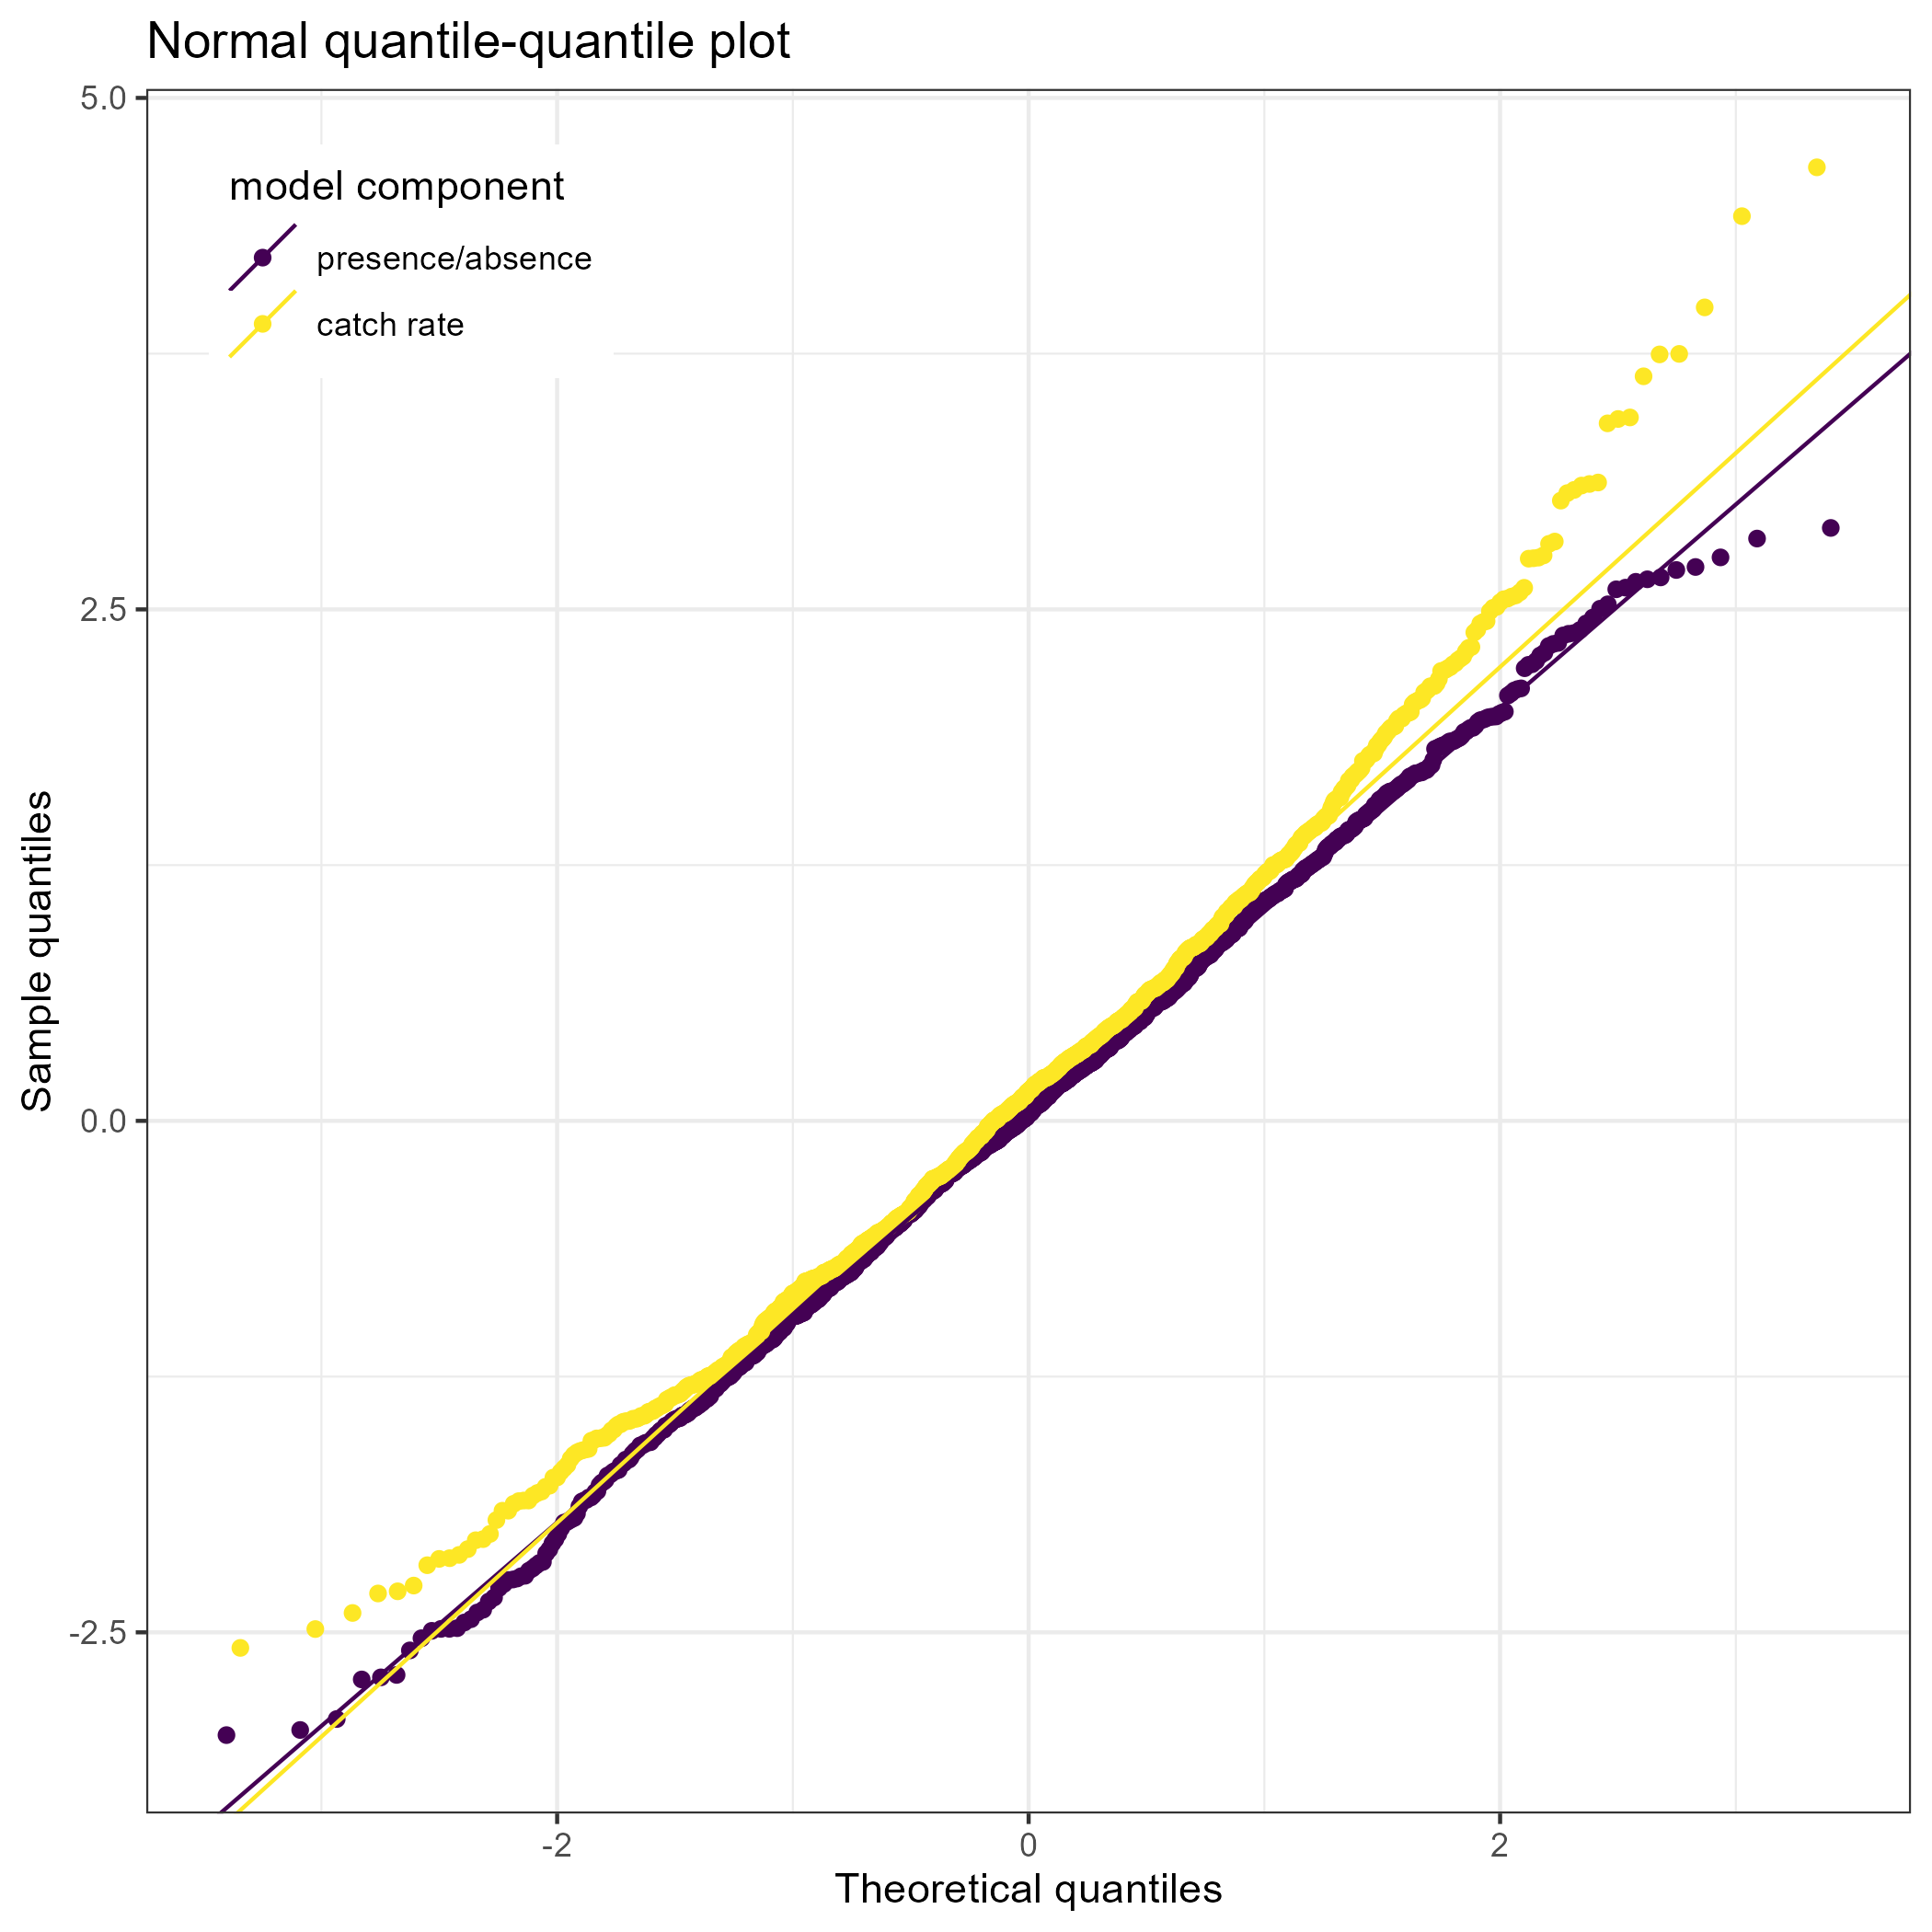
\includegraphics[width=1\linewidth,height=\textheight,keepaspectratio,alt={'Line plot with the theoretical quantiles along the x-axis and sample quantiles along the y-axis. The plot has a one-to-one line, points for the catch rate model, and points for the presence/absence model. The sample and theoretical quantiles for the presence/absence and catch rate models are roughly one to one with some departure at the larger quantiles for the catch rate model.'}]{figures/tri_early_qq.png}

}

\caption{\label{fig-qq-tri-early}QQ plot for the Triennial Survey for
the early period, 1980-1992.}

\end{figure}%

\pagebreak

\begin{figure}[H]

\centering{

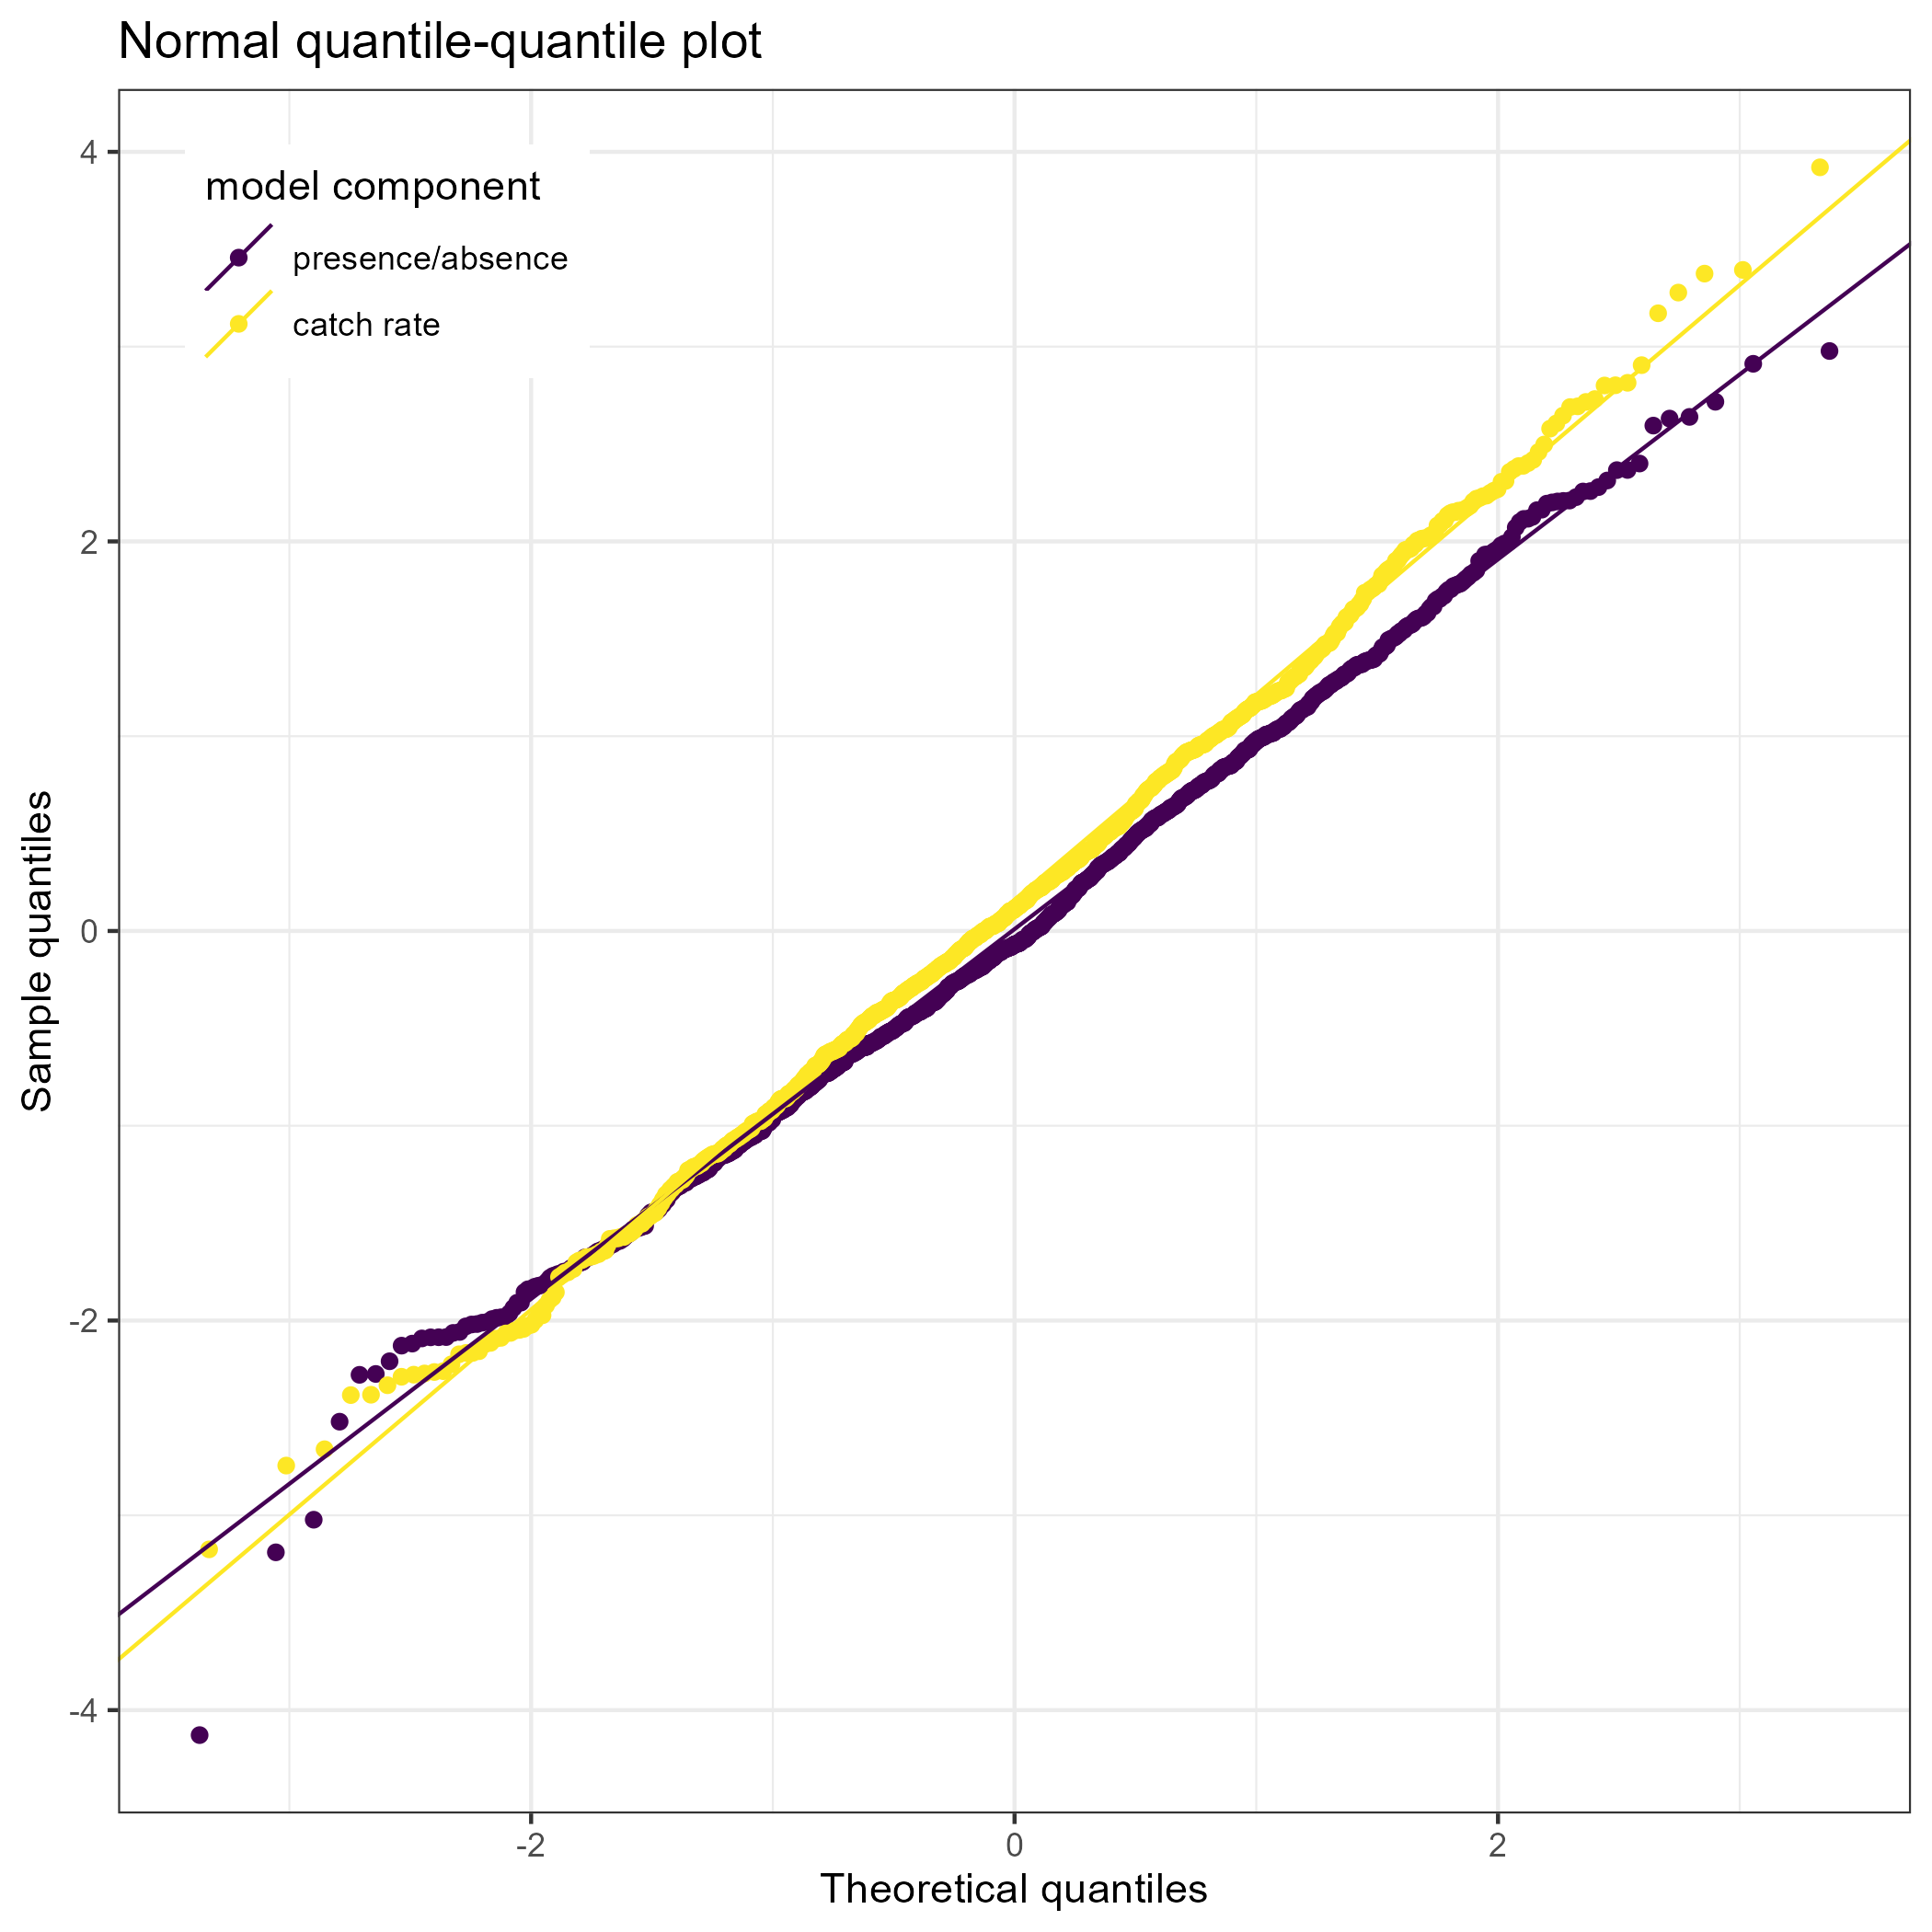
\includegraphics[width=1\linewidth,height=\textheight,keepaspectratio,alt={'Line plot with the theoretical quantiles along the x-axis and sample quantiles along the y-axis. The plot has a one-to-one line, points for the catch rate model, and points for the presence/absence model. The sample and theoretical quantiles for the presence/absence and catch rate models are roughly one to one with some departure at the larger quantiles for the catch rate model.'}]{figures/tri_late_qq.png}

}

\caption{\label{fig-qq-tri-late}QQ plot for the Triennial Survey for the
late period, 1995-2004.}

\end{figure}%

\pagebreak

\begin{figure}[H]

\centering{

\includegraphics[width=1\linewidth,height=\textheight,keepaspectratio,alt={'Line plot with year along the x-axis and relative abundance in metric tons along the y-axis with point and uncertainty intervals show for each year. The index slowly decreases from 1980 though 1989 and increases to highest point in 1992.'}]{../model/base_model/8.36_base_model/plots/index1_cpuedata_Triennial_Early.png}

}

\caption{\label{fig-index-tri-early}Relative index of abundance for the
Triennial Survey for the early period, 1980-1992.}

\end{figure}%

\pagebreak

\begin{figure}[H]

\centering{

\includegraphics[width=1\linewidth,height=\textheight,keepaspectratio,alt={'Line plot with year along the x-axis and relative abundance in metric tons along the y-axis with point and uncertainty intervals show for each year. The index is stable between 1995 and 1998 and increases for 2001 and 2004.'}]{../model/base_model/8.36_base_model/plots/index1_cpuedata_Triennial_Late.png}

}

\caption{\label{fig-index-tri-late}Relative index of abundance for the
Triennial Survey for the late period, 1995-2004.}

\end{figure}%

\pagebreak

\begin{figure}[H]

\centering{

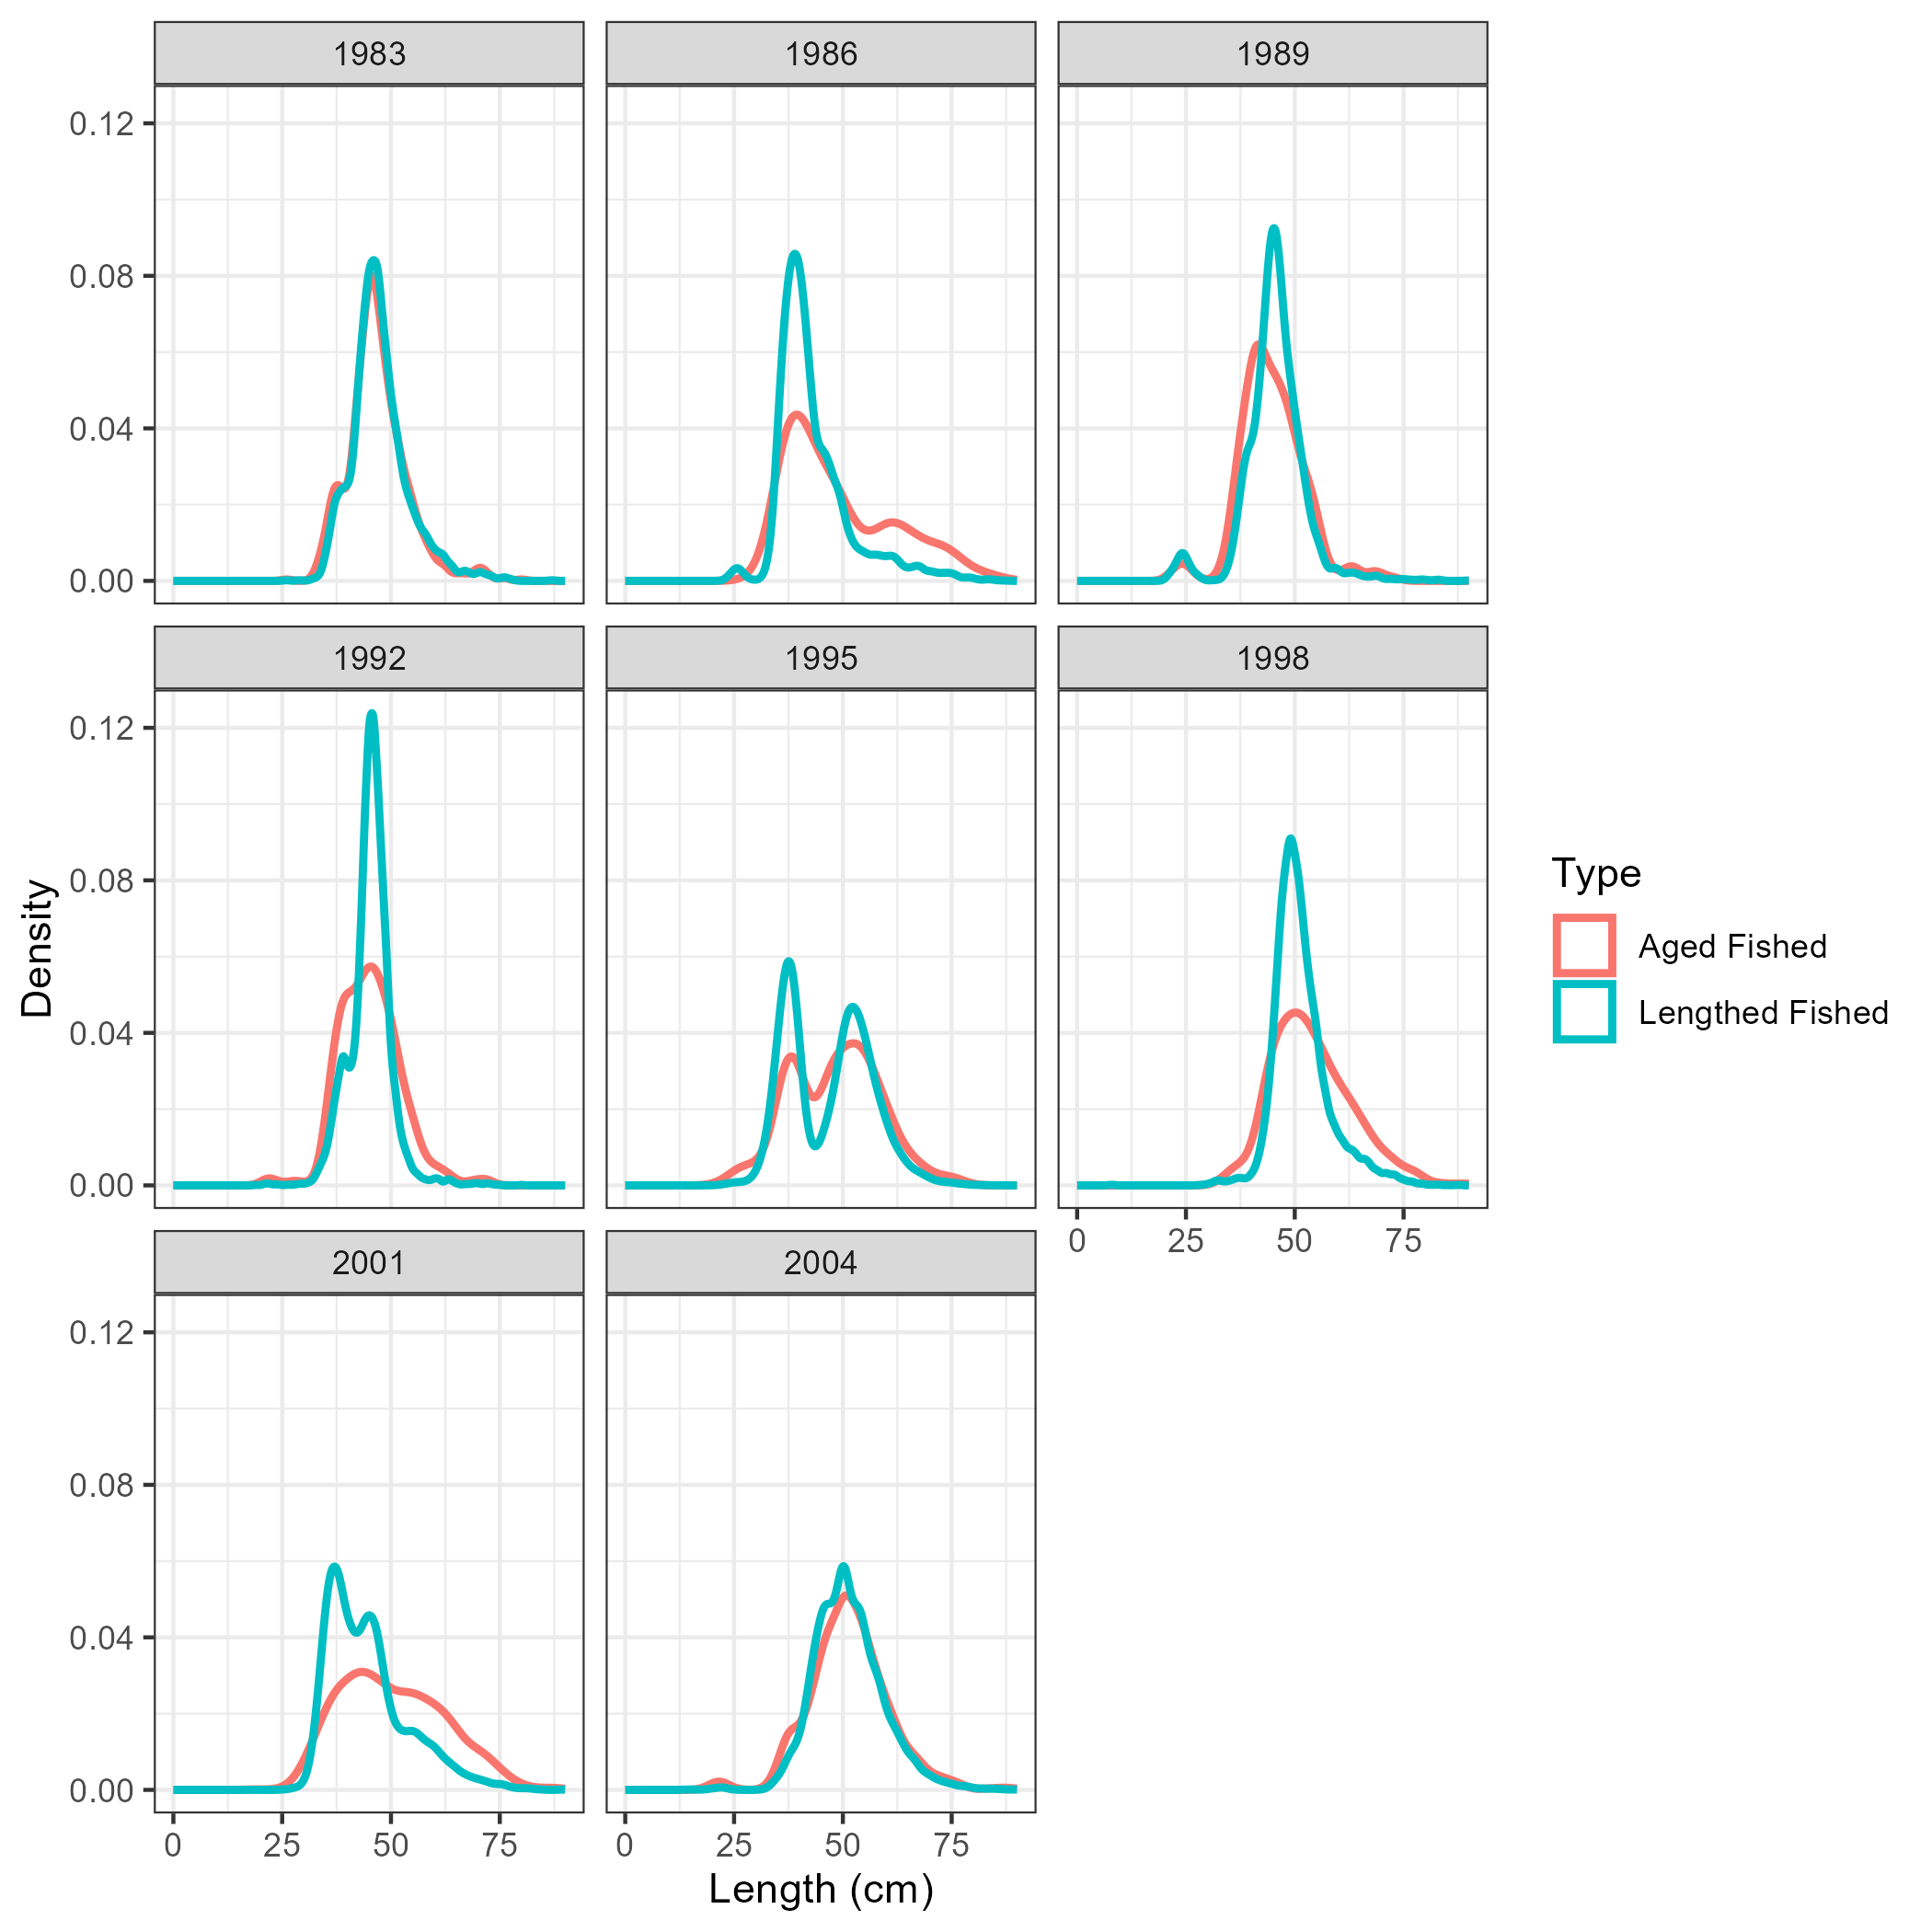
\includegraphics[width=1\linewidth,height=\textheight,keepaspectratio,alt={'Density plot with length in centimeters along the x-axis and density along the y-axis with panels for data by year. The density of all lengthed fish and the density of lengths of aged fish are shown by year to compare sample densities across lengths. The distribution of lengths for fish with ages has more weight in the upper tail for 1986, 1998, and 2001 compared to the distribution for all sablefish lengthed by the survey.'}]{figures/triennial_length_age_comparison.png}

}

\caption{\label{fig-data-tri-len-age}Comparison by year of the
distribution from all length data to the lengths from fish with ages
collected by the Triennial Survey.}

\end{figure}%

\begin{figure}[H]

\centering{

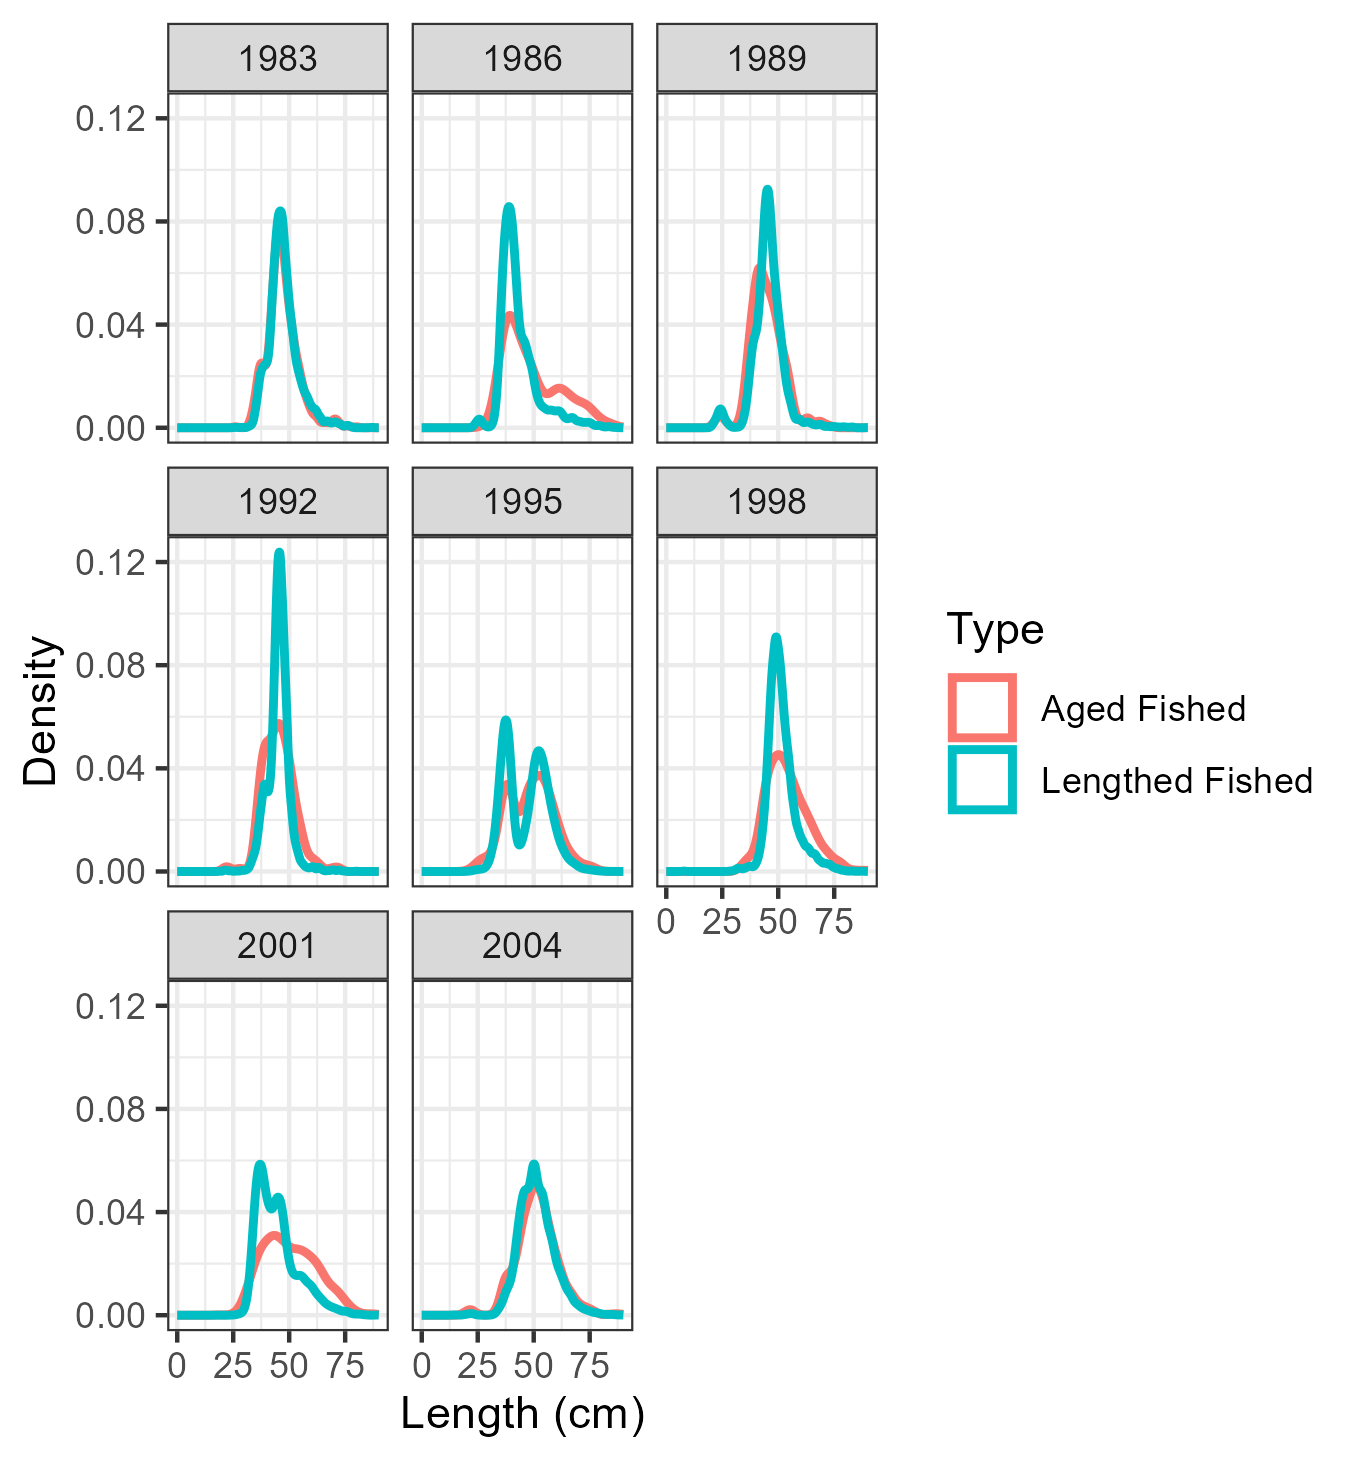
\includegraphics[width=1\linewidth,height=\textheight,keepaspectratio,alt={'Data point plot with latitude along the x-axis and depth in meters along the y-axis with panels by year. Data plotted for each positive tow for sablefish and where age data were collected by latitude and depth. The distribution of tows by latitude and depth where ages were collected did not appear to be randomly distributed for all tows with sablefish for 1983, 1986, and 1998.'}]{figures/triennial_positive_tow_bds.png}

}

\caption{\label{fig-data-tri-tows}Tow location by latitude and year
where lengths were sampled (black open circles) compared to location of
available age data (red filled triangles) from the Triennial Survey.}

\end{figure}%

\begin{figure}[H]

\centering{

\includegraphics[width=1\linewidth,height=\textheight,keepaspectratio,alt={'Plot with year on the x-axis and age in years on the y-axis with open circles indicating the proportion of samples by sex at each age for each year with data. The majority of observations for males and females were you fish less than five years of age.'}]{../model/base_model/8.36_base_model/plots/comp_agedat_bubflt7mkt0.png}

}

\caption{\label{fig-data-tri-early}Age compositions by year from the
early Triennial Survey. Females are shown in red and males in blue.}

\end{figure}%

\pagebreak

\begin{figure}[H]

\centering{

\includegraphics[width=1\linewidth,height=\textheight,keepaspectratio,alt={'Plot with year on the x-axis and age in years on the y-axis with open circles indicating the proportion of samples by sex at each age for each year with data. The majority of observations for males and females were you fish less than five years of age.'}]{../model/base_model/8.36_base_model/plots/comp_agedat_bubflt8mkt0.png}

}

\caption{\label{fig-data-tri-late}Age compositions by year from the late
Triennial Survey. Females are shown in red and males in blue}

\end{figure}%

\pagebreak

\begin{figure}[H]

\centering{

\includegraphics[width=1\linewidth,height=\textheight,keepaspectratio,alt={'Line plot with year along the x-axis and mean age along the y-axis with median values and quantiles shown for each year of data. The mean age for 1983, 1989, and 1994 was approximately four years of age.'}]{../model/base_model/8.36_base_model/plots/comp_agedat_data_weighting_TA1-8_Triennial_Early.png}

}

\caption{\label{fig-data-tri-early-mean-age}Mean age for early period of
Triennial Survey with 95 percent confidence intervals based on current
sample sizes.}

\end{figure}%

\pagebreak

\begin{figure}[H]

\centering{

\includegraphics[width=1\linewidth,height=\textheight,keepaspectratio,alt={'Line plot with year along the x-axis and mean age along the y-axis with median values and quantiles shown for each year of data. The mean age in 1995 was between 6.5 and seven years of age and decreased in 2004 for approxamately 5.5 years of age.'}]{../model/base_model/8.36_base_model/plots/comp_agedat_data_weighting_TA1-8_Triennial_Late.png}

}

\caption{\label{fig-data-tri-late-mean-age}Mean age for late period of
Triennial Survey with 95 percent confidence intervals based on current
sample sizes.}

\end{figure}%

\pagebreak

\begin{figure}[H]

\centering{

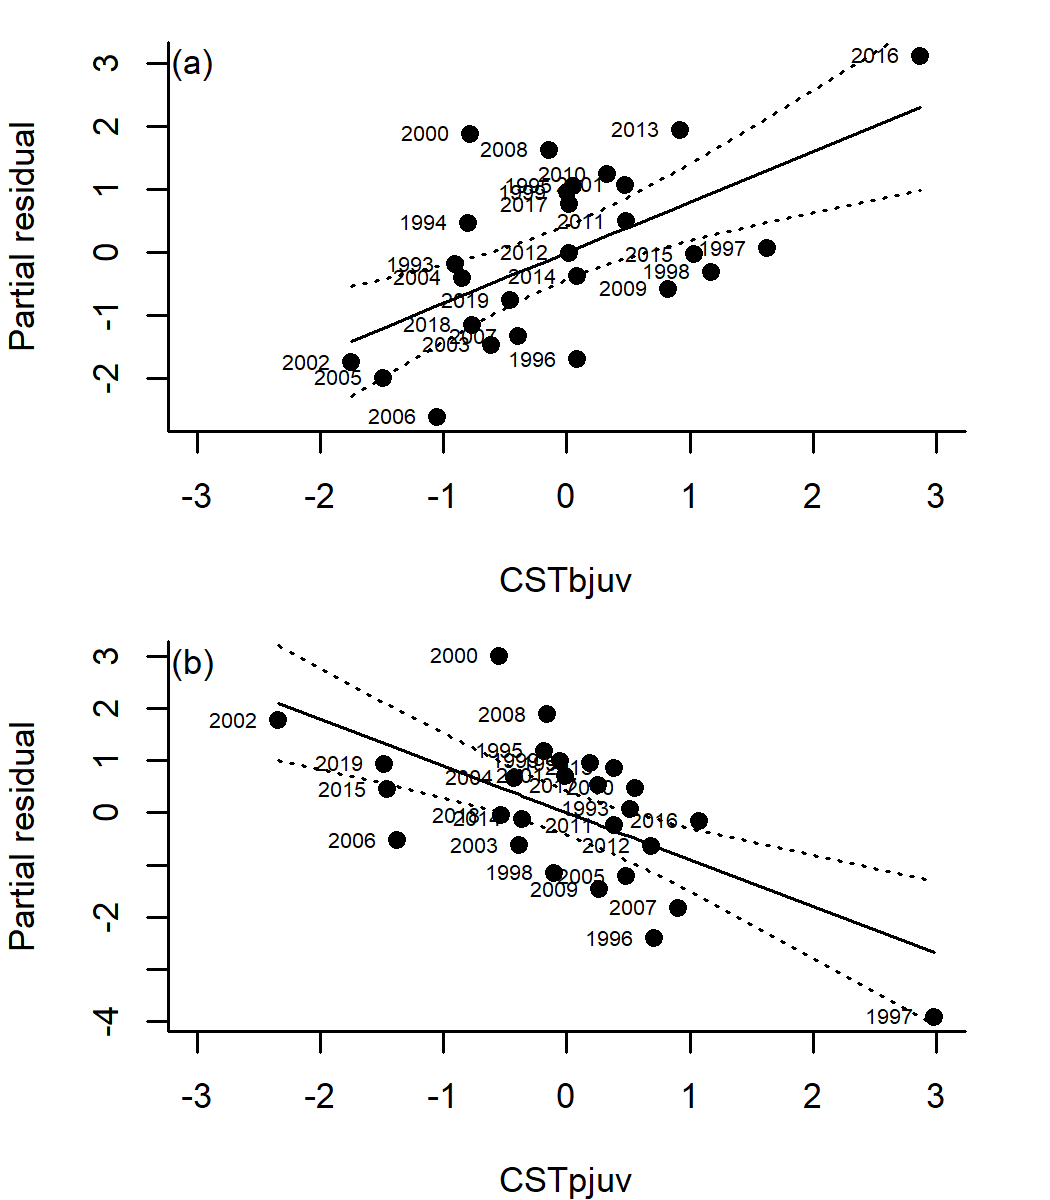
\includegraphics[width=1\linewidth,height=\textheight,keepaspectratio,alt={'Data plot with ecosystem factor along the x-axis and partial residual along the y-axis with data points by year. Recruitment appears to be positively correlated with cross shelf transport during the benthic juvenile stage and negatively correlated with cross shelf transport during the pelagive juvenile stage.'}]{figures/gloyrs_figure_4.png}

}

\caption{\label{fig-glorys-terms}Partial residual plots of GLORYS
predictors. CST = cross-shelf transport, T = temperature, spawn =
spaning stage, pjuv = pelagic juvenile, and bjuv = benthic juvenile
stage.}

\end{figure}%

\begin{figure}[H]

\centering{

\includegraphics[width=1\linewidth,height=\textheight,keepaspectratio,alt={'Line plot with year along the x-axis and recruitment index in log-space along the y-axis. Recruitment is estimated to be above average in 2020, 2021, 2023, and 2024 and below average in 2022.'}]{../model/base_model/8.36_base_model/plots/index1_cpuedata_Recruitment_Index.png}

}

\caption{\label{fig-rec-index}Recruitment deviation index.}

\end{figure}%

\pagebreak

\begin{figure}[H]

\centering{

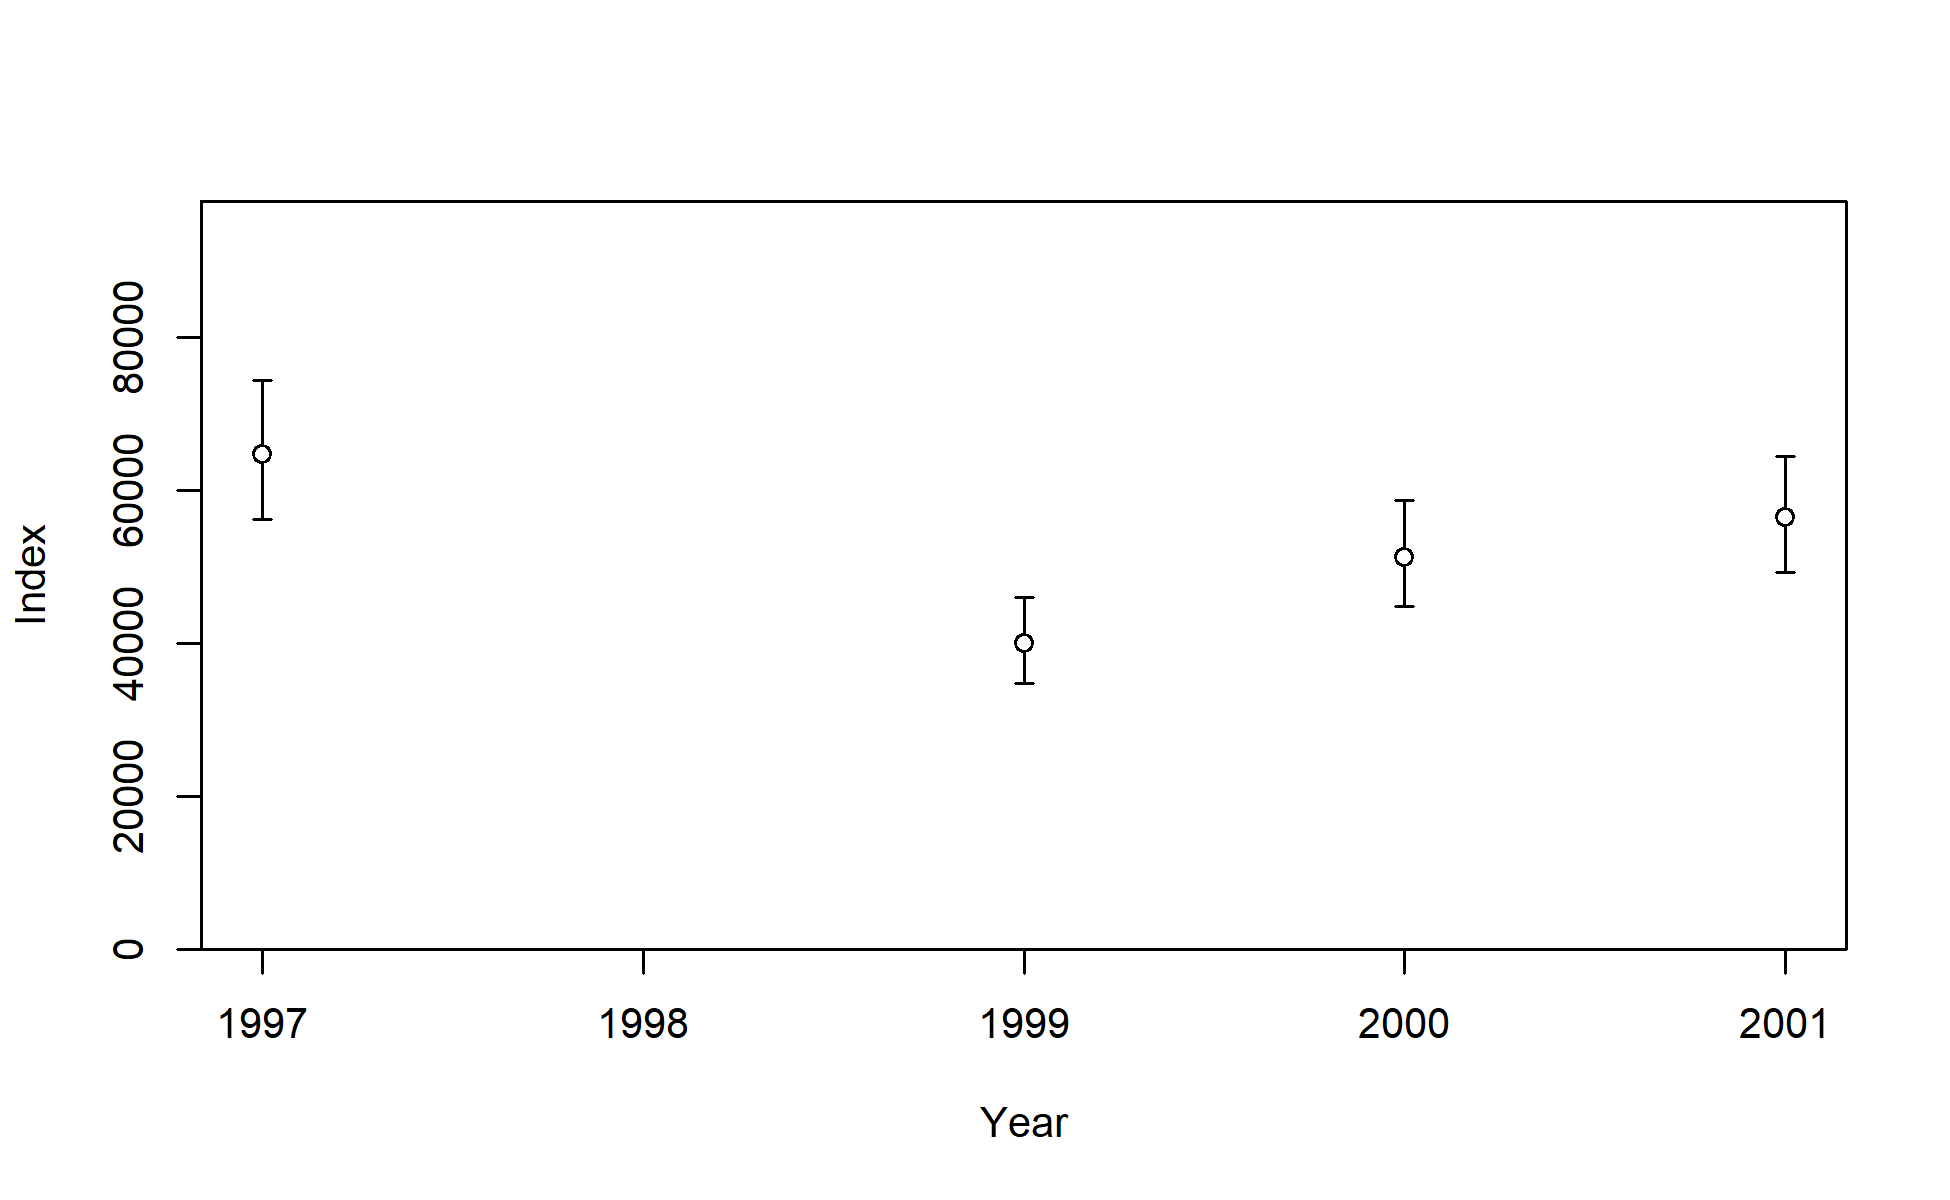
\includegraphics[width=1\linewidth,height=\textheight,keepaspectratio,alt={'Line plot with year along the x-axis and relative abundance in metric tons along the y-axis with point and uncertainty intervals show for each year. The index declines from 1997 to 1999 and then slowly increase in 2000 and 2001.'}]{figures/index1_cpuedata_AKFSC_SLOPE.png}

}

\caption{\label{fig-data-afslope-index}Relative index of abundance for
the AFSC Slope Survey.}

\end{figure}%

\begin{figure}[H]

\centering{

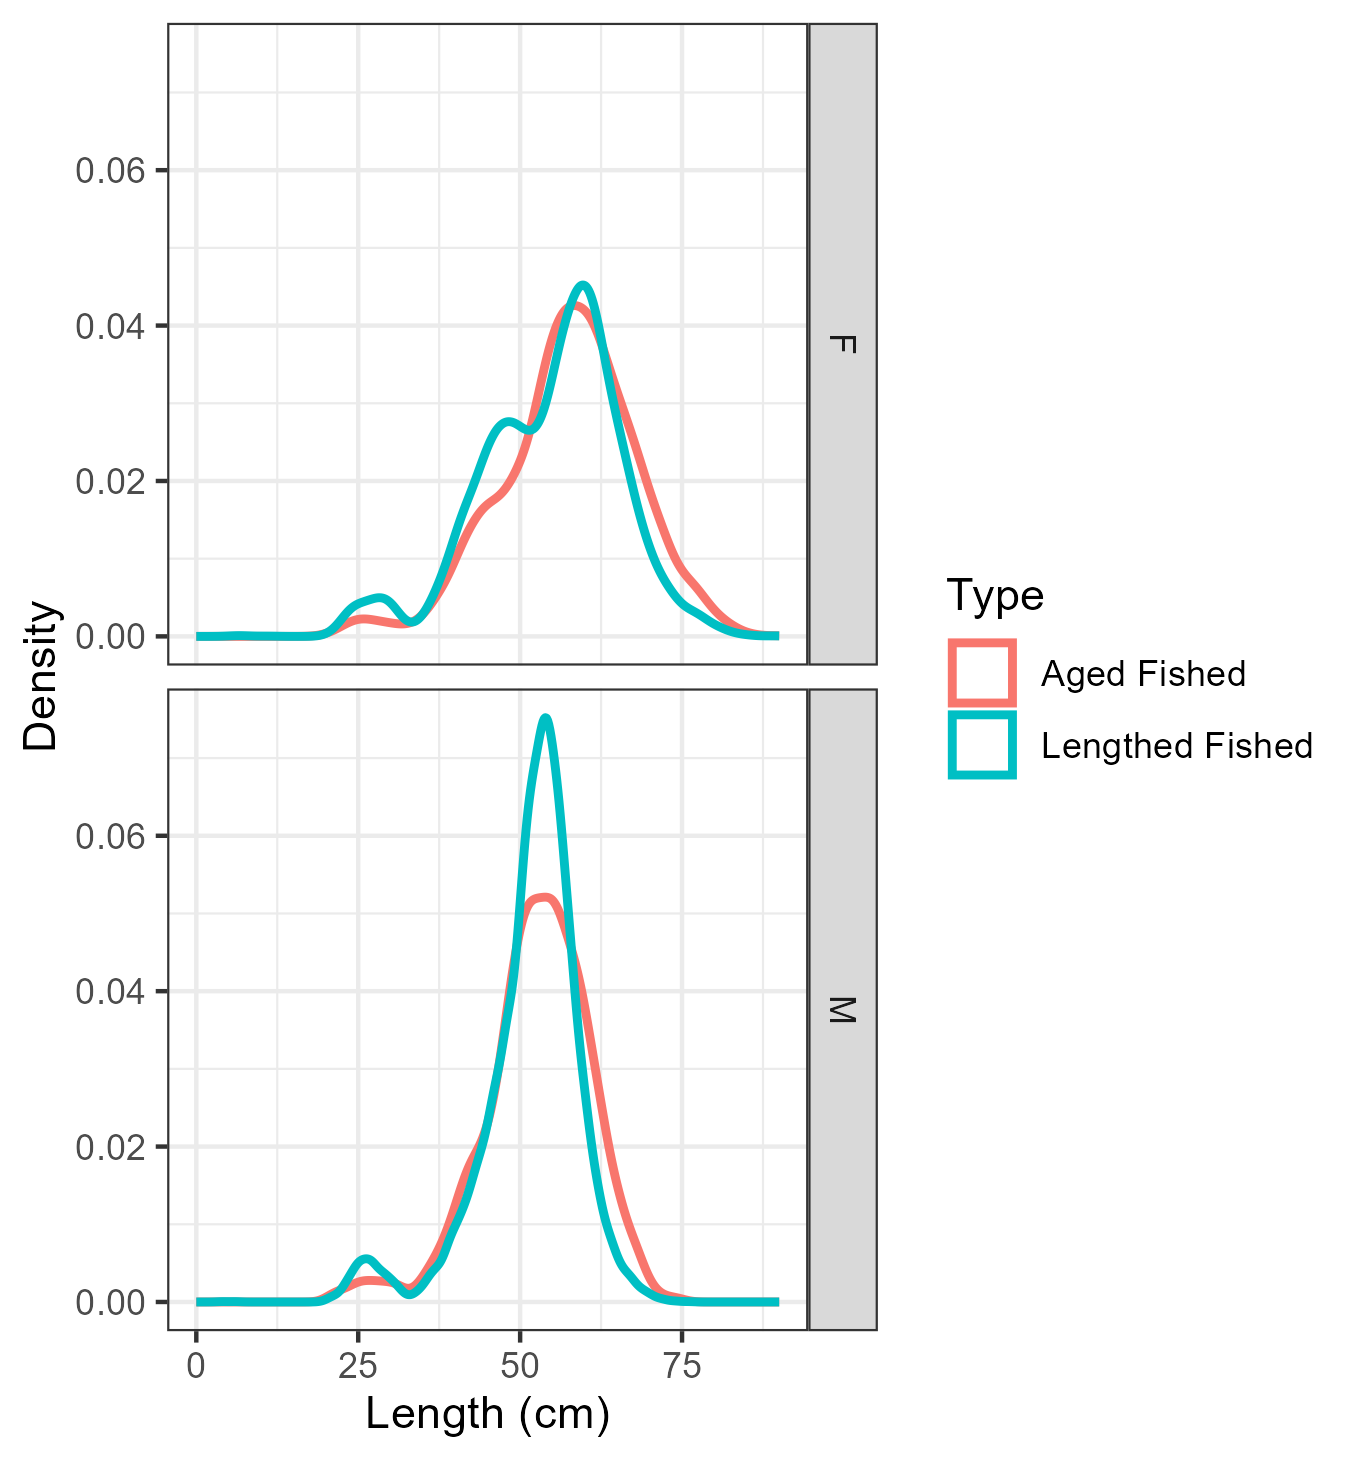
\includegraphics[width=1\linewidth,height=\textheight,keepaspectratio,alt={'Line plot with length in centimeters along the x-axis and density along the x-axis with data shown by sex.  The density of all fished lengthed and lengthed fish with ages are compared for departure in the distribution by length. The density for lengthed fish with ages was greater than all fished lengthed for larger fish sampled by the survey.'}]{figures/afsc_slope_length_age_comparison.png}

}

\caption{\label{fig-data-afslope-len-age}Comparison of the distribution
from all length data to the lengths from fish with ages collected by the
AFSC Slope Survey.}

\end{figure}%

\subsection{Biology}\label{biology}

\begin{figure}[H]

\centering{

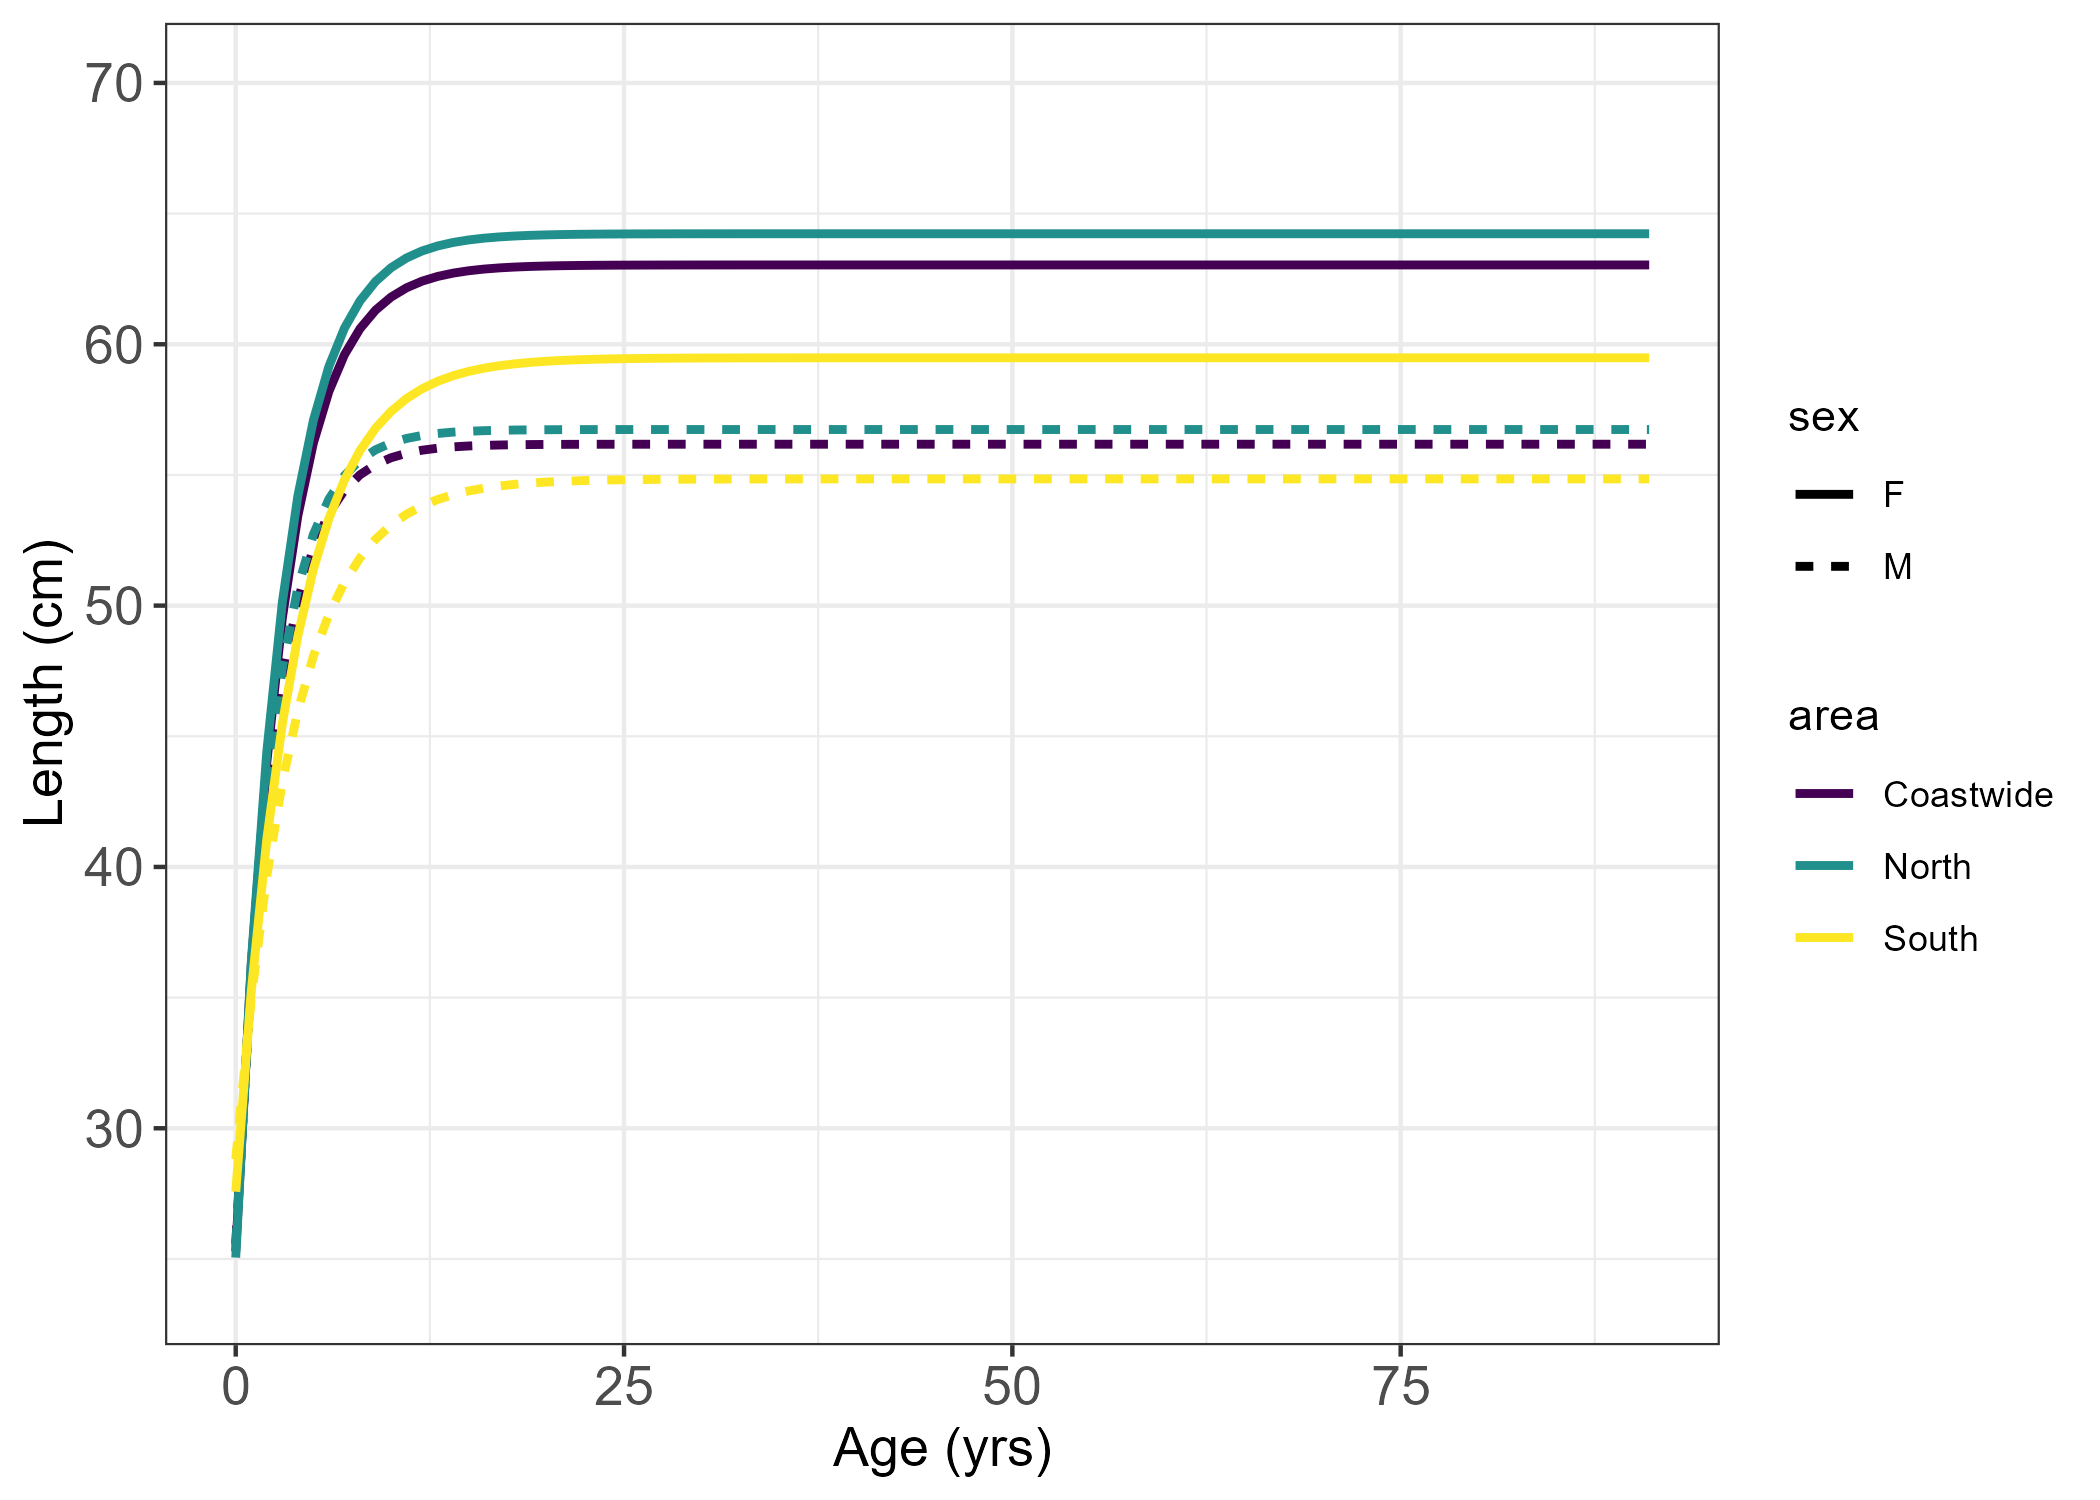
\includegraphics[width=1\linewidth,height=\textheight,keepaspectratio,alt={'oastwide, north, and south. Females are estimated to reach larger maximum sizes compared to males and fish in the north are estimated to grow to larger sizes for both sexes compared to fish in the south.  The coastwide asymptotic size for females is estimated to be approximate 63 cm with males reaching a maximum size of approximately 55 cm. Sablefish of both sexes reach asymptotic size around 12 years of age.'}]{figures/external_growth.png}

}

\caption{\label{fig-external-growth}Estimated length-at-age coastwide
and by area for females (solid lines) and males (dashed lines) north and
south of 36° N. latitude.}

\end{figure}%

\begin{figure}[H]

\centering{

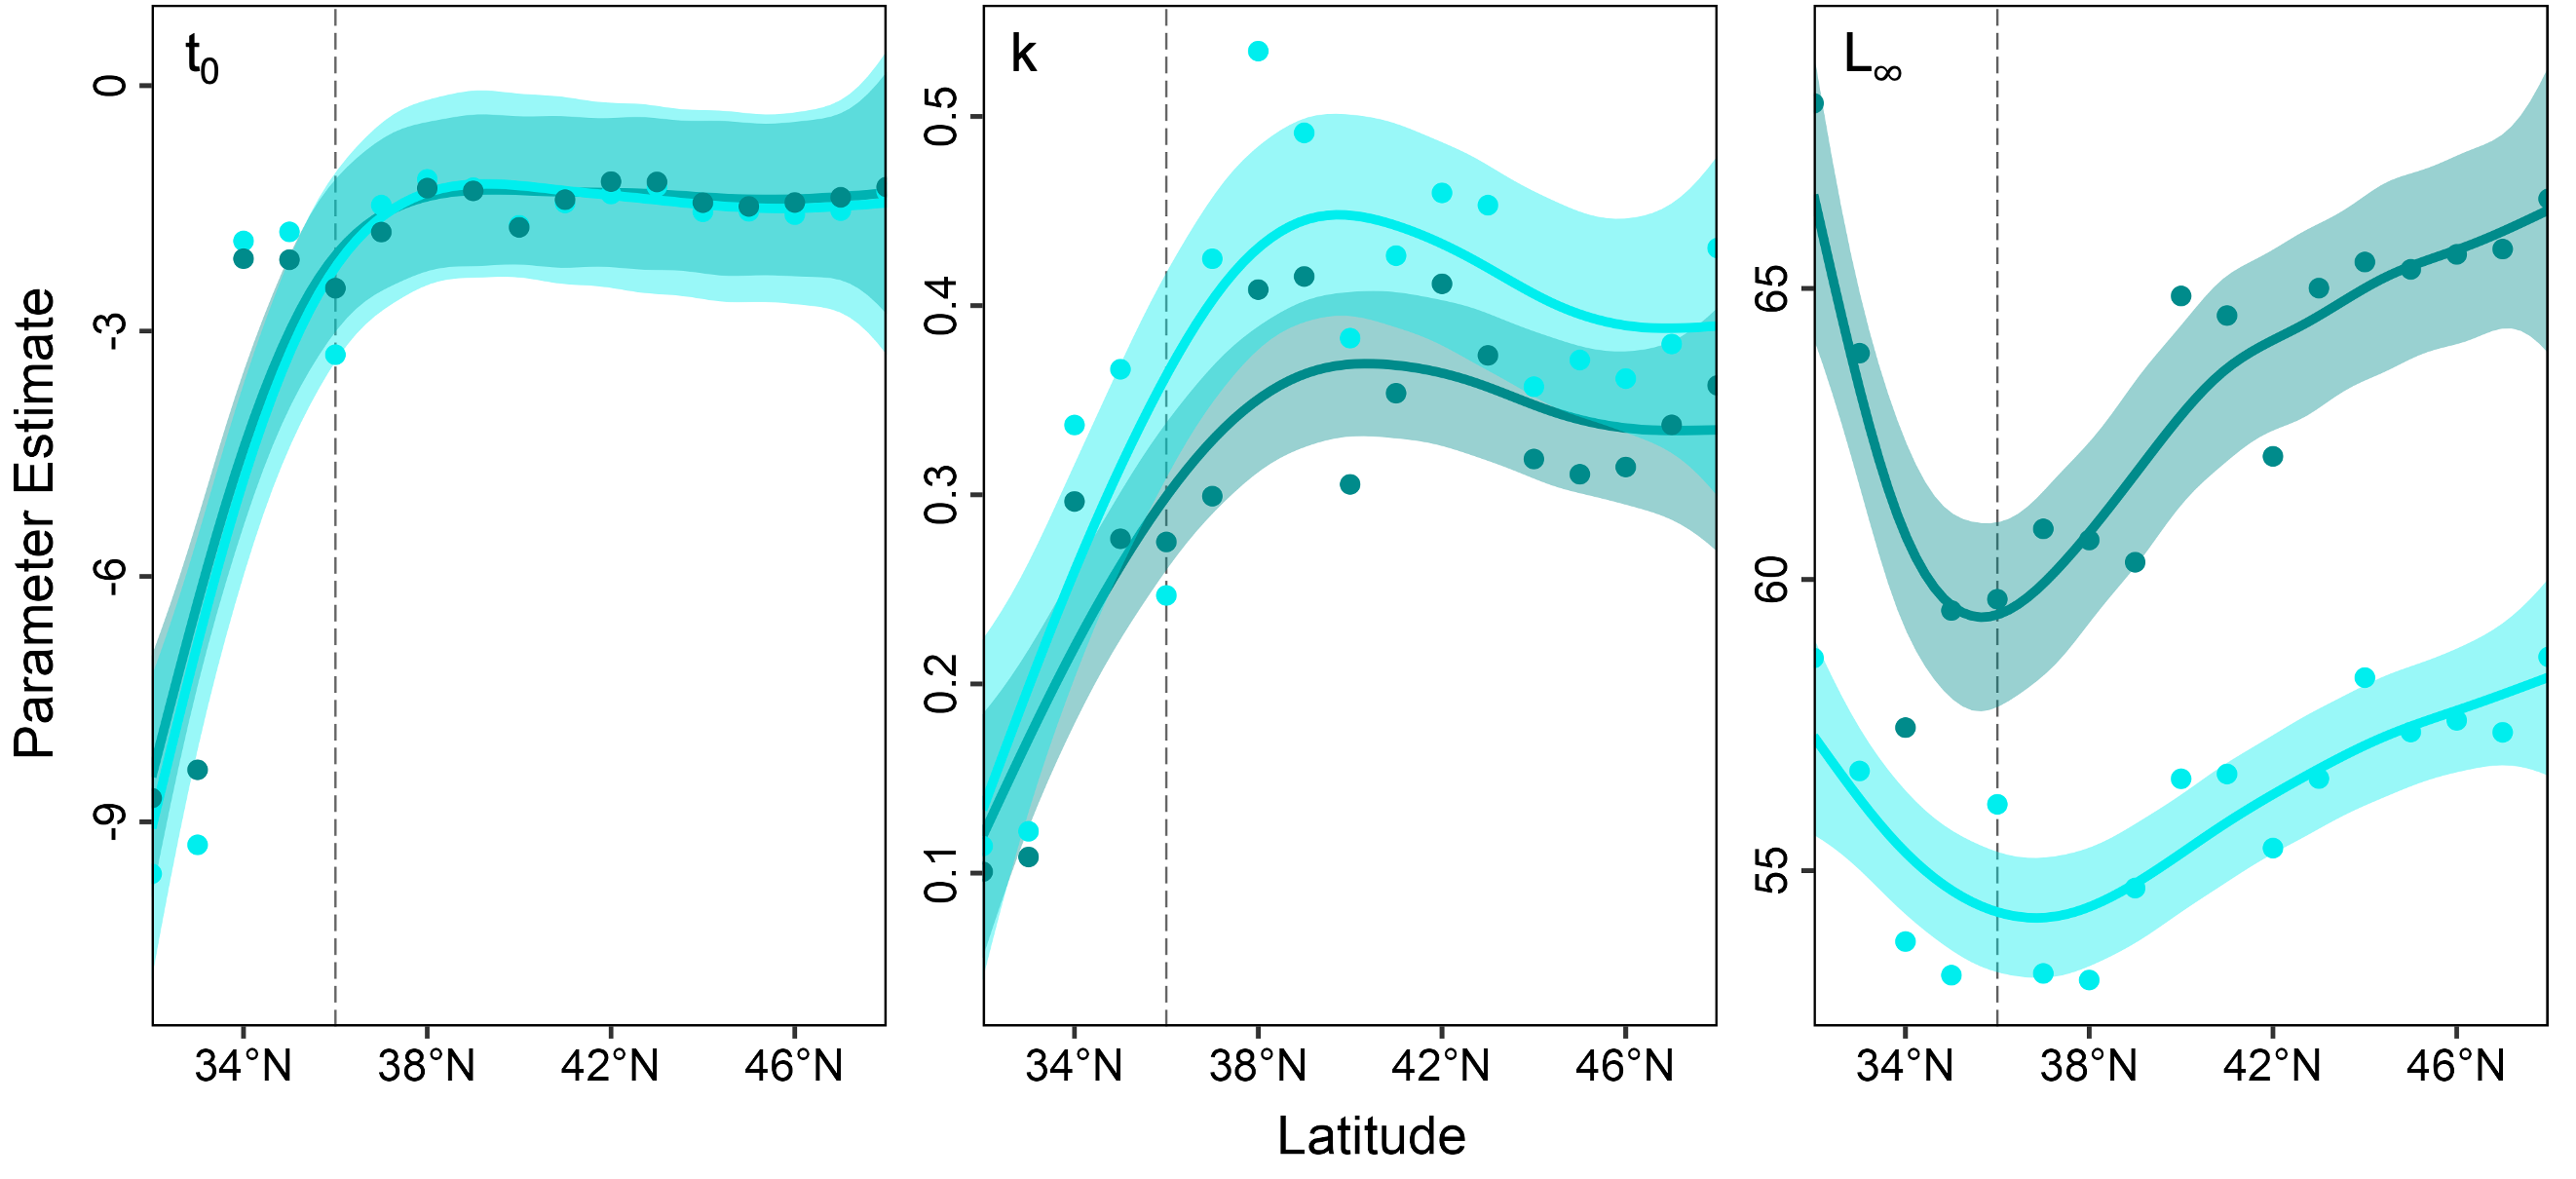
\includegraphics[width=1\linewidth,height=\textheight,keepaspectratio,alt={'Line plot with latitude along the x-axis and parameter estimate along the y-axis with separate panels for t0, k, and asymptotic length. The growth parameters generally increase with latitude.'}]{figures/external_growth_lat.png}

}

\caption{\label{fig-external-growth-lat}Latitudinal variation in
sex-specific von Bertalanffy growth parameters (\(t_0\): length at age
0, \emph{k}: growth coefficient, L∞: asymptotic length). Dashed
horizontal line denotes 36° N. latitude. Predicted using the NWFSC West
Coast Groundfish Bottom Trawl Survey data between 2003 and 2024. The
darker color represents females and the lighter color represents males.}

\end{figure}%

\pagebreak

\begin{figure}[H]

\centering{

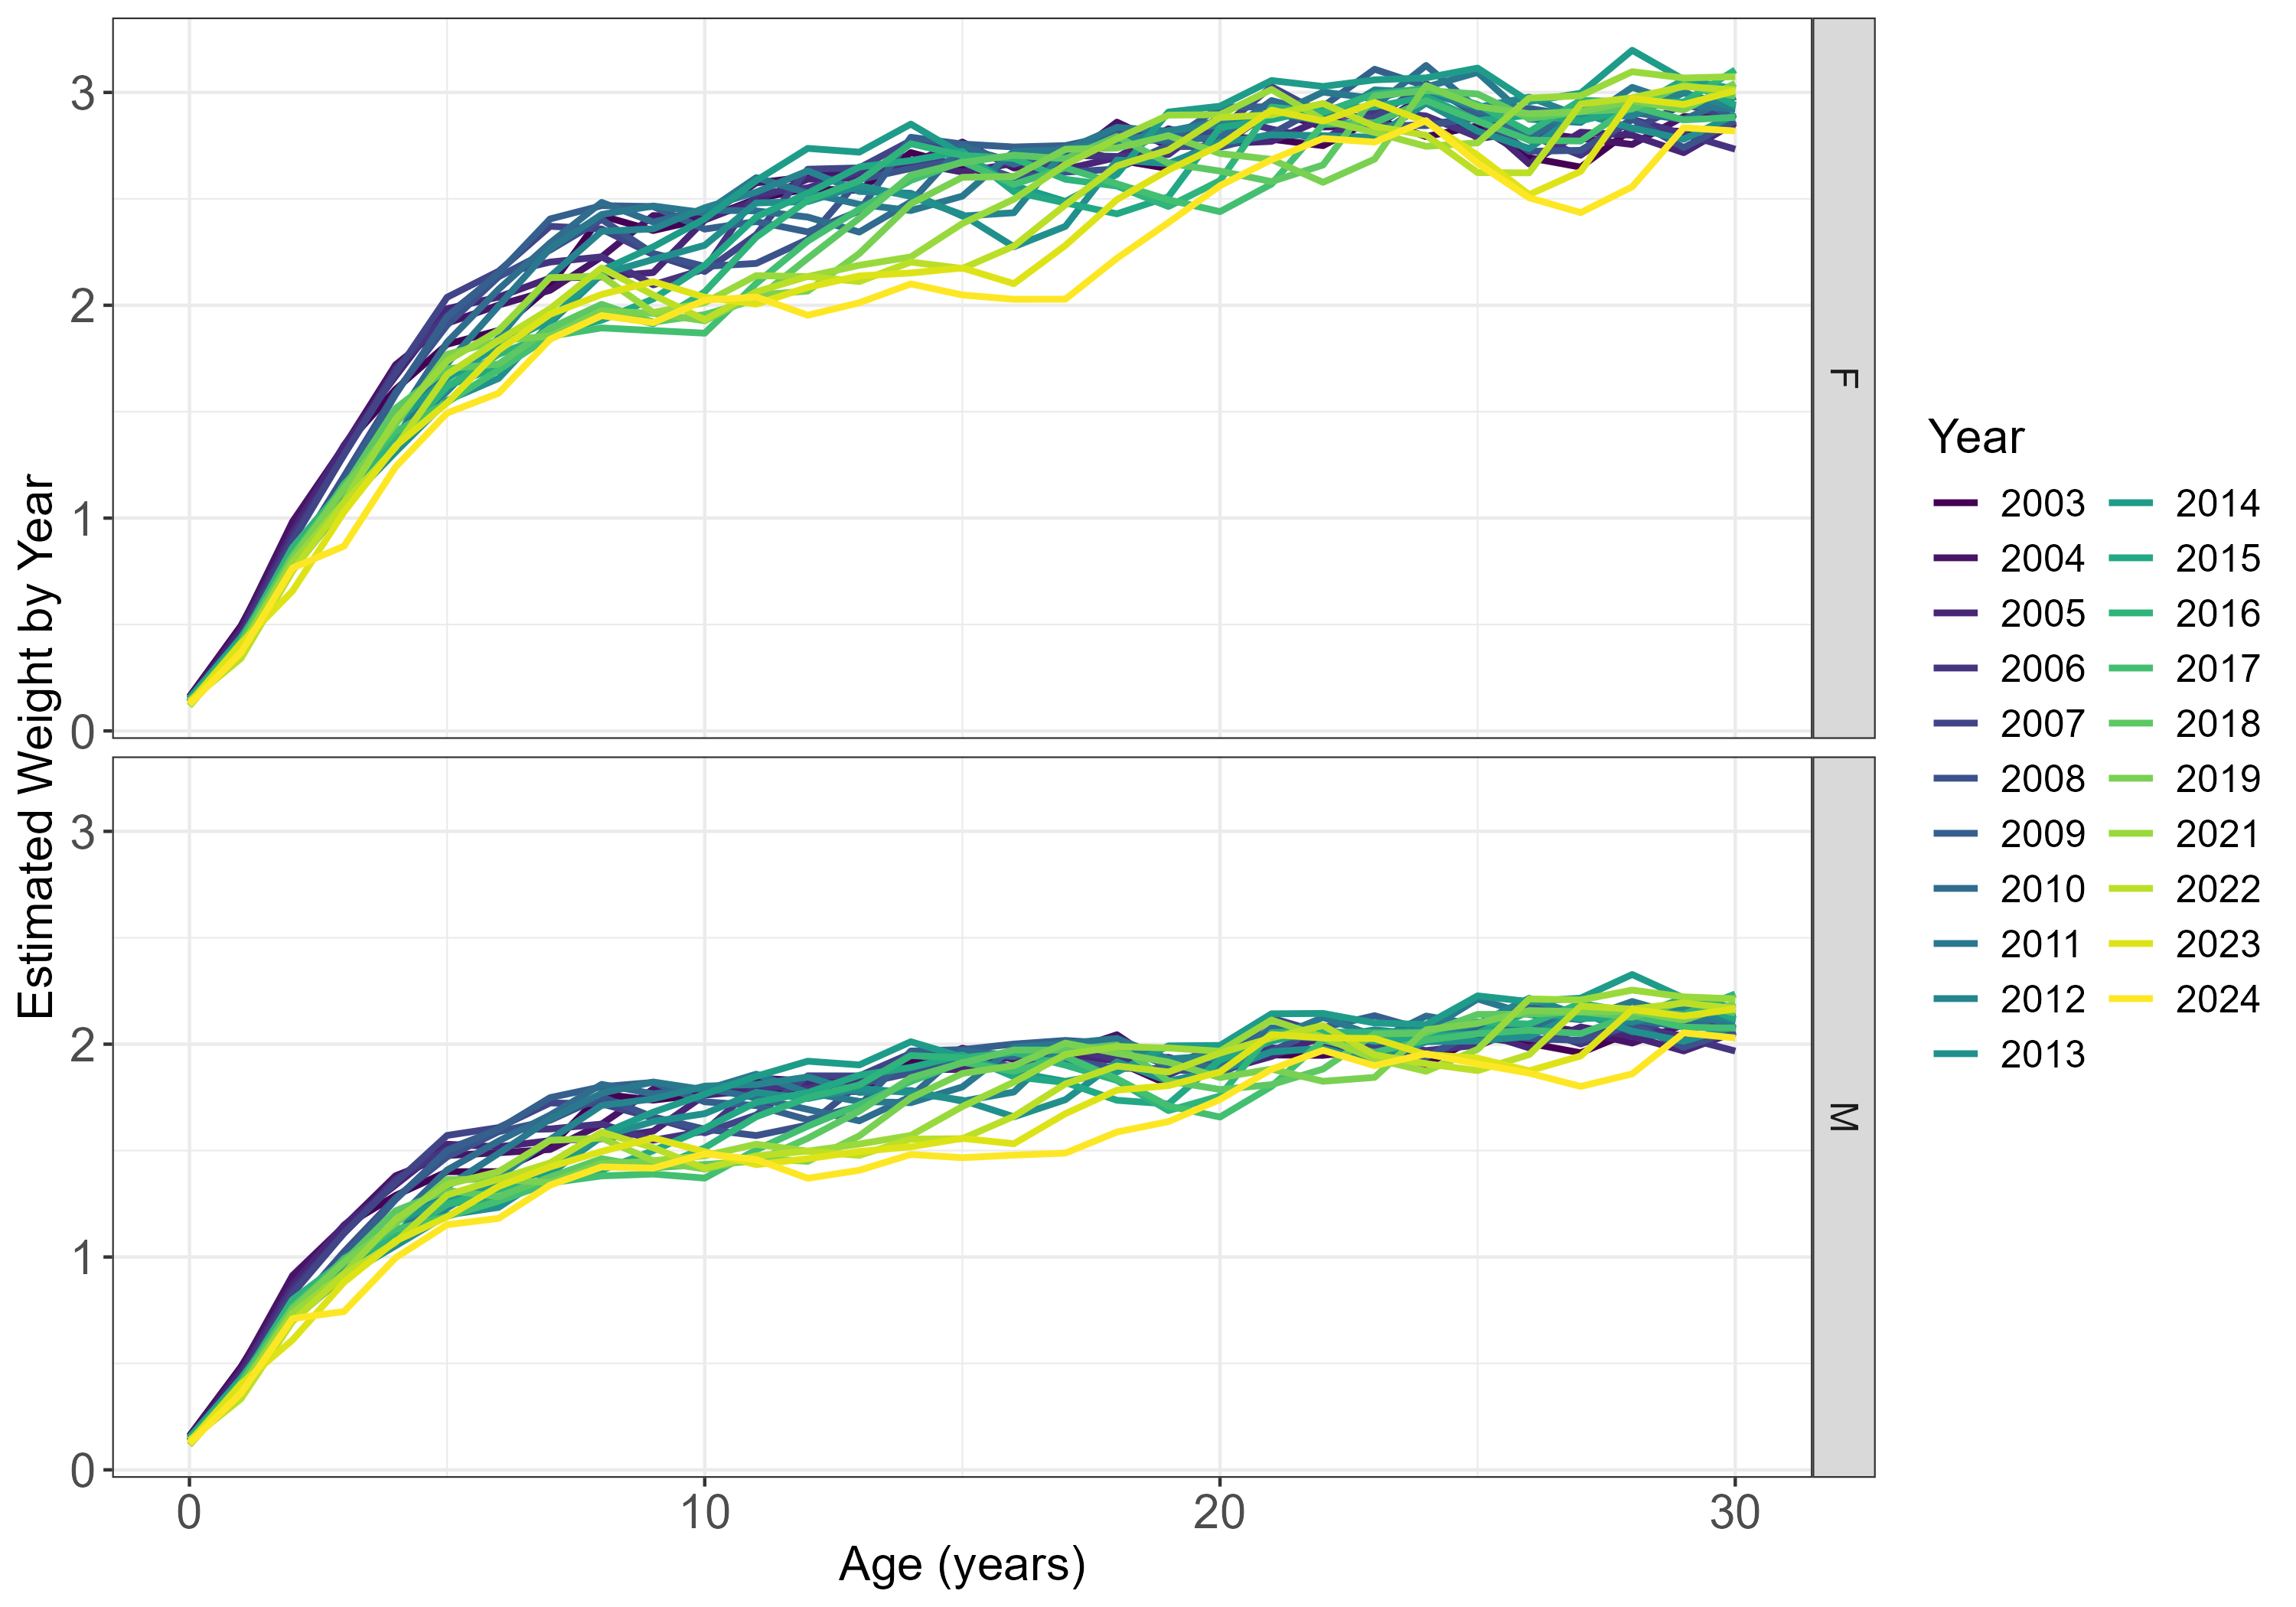
\includegraphics[width=1\linewidth,height=\textheight,keepaspectratio,alt={'Line plot with age in years along the x-axis and estimated weight along the y-axis with a line for each data year and separate panels by sex. Weight at age by sex varies by year with females reaching larger maximum weights compared to males.'}]{figures/year_wt_at_age_estimate_survey.png}

}

\caption{\label{fig-data-watage}Estimated weight-at-age by year and
sex.}

\end{figure}%

\pagebreak

\begin{figure}[H]

\centering{

\includegraphics[width=1\linewidth,height=\textheight,keepaspectratio,alt={'Heatplot with age in years along the x-axis and year along the y-axis with weight-at-age shown in colors. Data by sex are plotted separately. Weight at age by sex varies by year with females reaching larger maximum weights compared to males. Females reach a maximum weight-at-age greater than 3.0 kg by the age of 20.'}]{../model/base_model/8.36_base_model/plots/bio5_weightatsize.png}

}

\caption{\label{fig-weight-at-age-female}Female weight-at-age by year.}

\end{figure}%

\begin{figure}[H]

\centering{

\includegraphics[width=1\linewidth,height=\textheight,keepaspectratio,alt={'Heatplot with age in years along the x-axis and year along the y-axis with weight-at-age shown in colors. Data by sex are plotted separately. Weight at age by sex varies by year with females reaching larger maximum weights compared to males. Males reach a maximum weight-at-age greater than 2.0 kg by the age of 25.'}]{../model/base_model/8.36_base_model/plots/bio5_weightatsize2.png}

}

\caption{\label{fig-weight-at-age-male}Male weight-at-age by year.}

\end{figure}%

\begin{figure}[H]

\centering{

\includegraphics[width=1\linewidth,height=\textheight,keepaspectratio,alt={'Data plotted with age in years along the x-axis and functional maturity along the y-axis with data plotted separately north and south. Age associated with immature and mature fish by area. In the north fish are mature at younger ages more frequently compared to fish in the south.'}]{SAR_USWC_sablefish_skeleton_files/figure-pdf/fig-maturity-data-1.pdf}

}

\caption{\label{fig-maturity-data}Samples by age that were determined to
be functionally mature and immature north and south of 36° N. latitude.
Immature fish have a functional maturity of 0 and mature fish have a
functional maturity of 1. Blue vertical dashed line at age 7.}

\end{figure}%

\newpage

\begin{figure}[H]

\centering{

\includegraphics[width=1\linewidth,height=\textheight,keepaspectratio,alt={'Line plot with age in years along the x-axis and probability mature along the y-axis with three lines for weighted estimates coastwide, south, and north. Maturity in the south is later compared to fish in the north with the biomass weighted maturity curve being slightly right shifted compared to the north maturity curve. Weighted coastwide data has age at 50 percent mature between 6 and 7 years of age and 100 percent mature by 10 years of age.'}]{SAR_USWC_sablefish_skeleton_files/figure-pdf/fig-maturity-ogive-1.pdf}

}

\caption{\label{fig-maturity-ogive}Estimated maturity-at-age by area and
the biomass weighted coastwide (Spatial) maturity curve and north
(Spatial-N) and south (Spatial-S) of 36° N. latitude.}

\end{figure}%

\newpage

\begin{figure}[H]

\centering{

\includegraphics[width=1\linewidth,height=\textheight,keepaspectratio,alt={'Heatplot with age in years along the x-ax-s and year along the y-axis with the product of maturity and fecundity.  Fecundity is equal to weight-at-age. Spawning output varies by year from 2003 through 2024.'}]{../model/base_model/8.36_base_model/plots/bio6_maturity.png}

}

\caption{\label{fig-fecundity-maturity}Spawning output at age based upon
maturity and fecundity.}

\end{figure}%

\begin{figure}[H]

\centering{

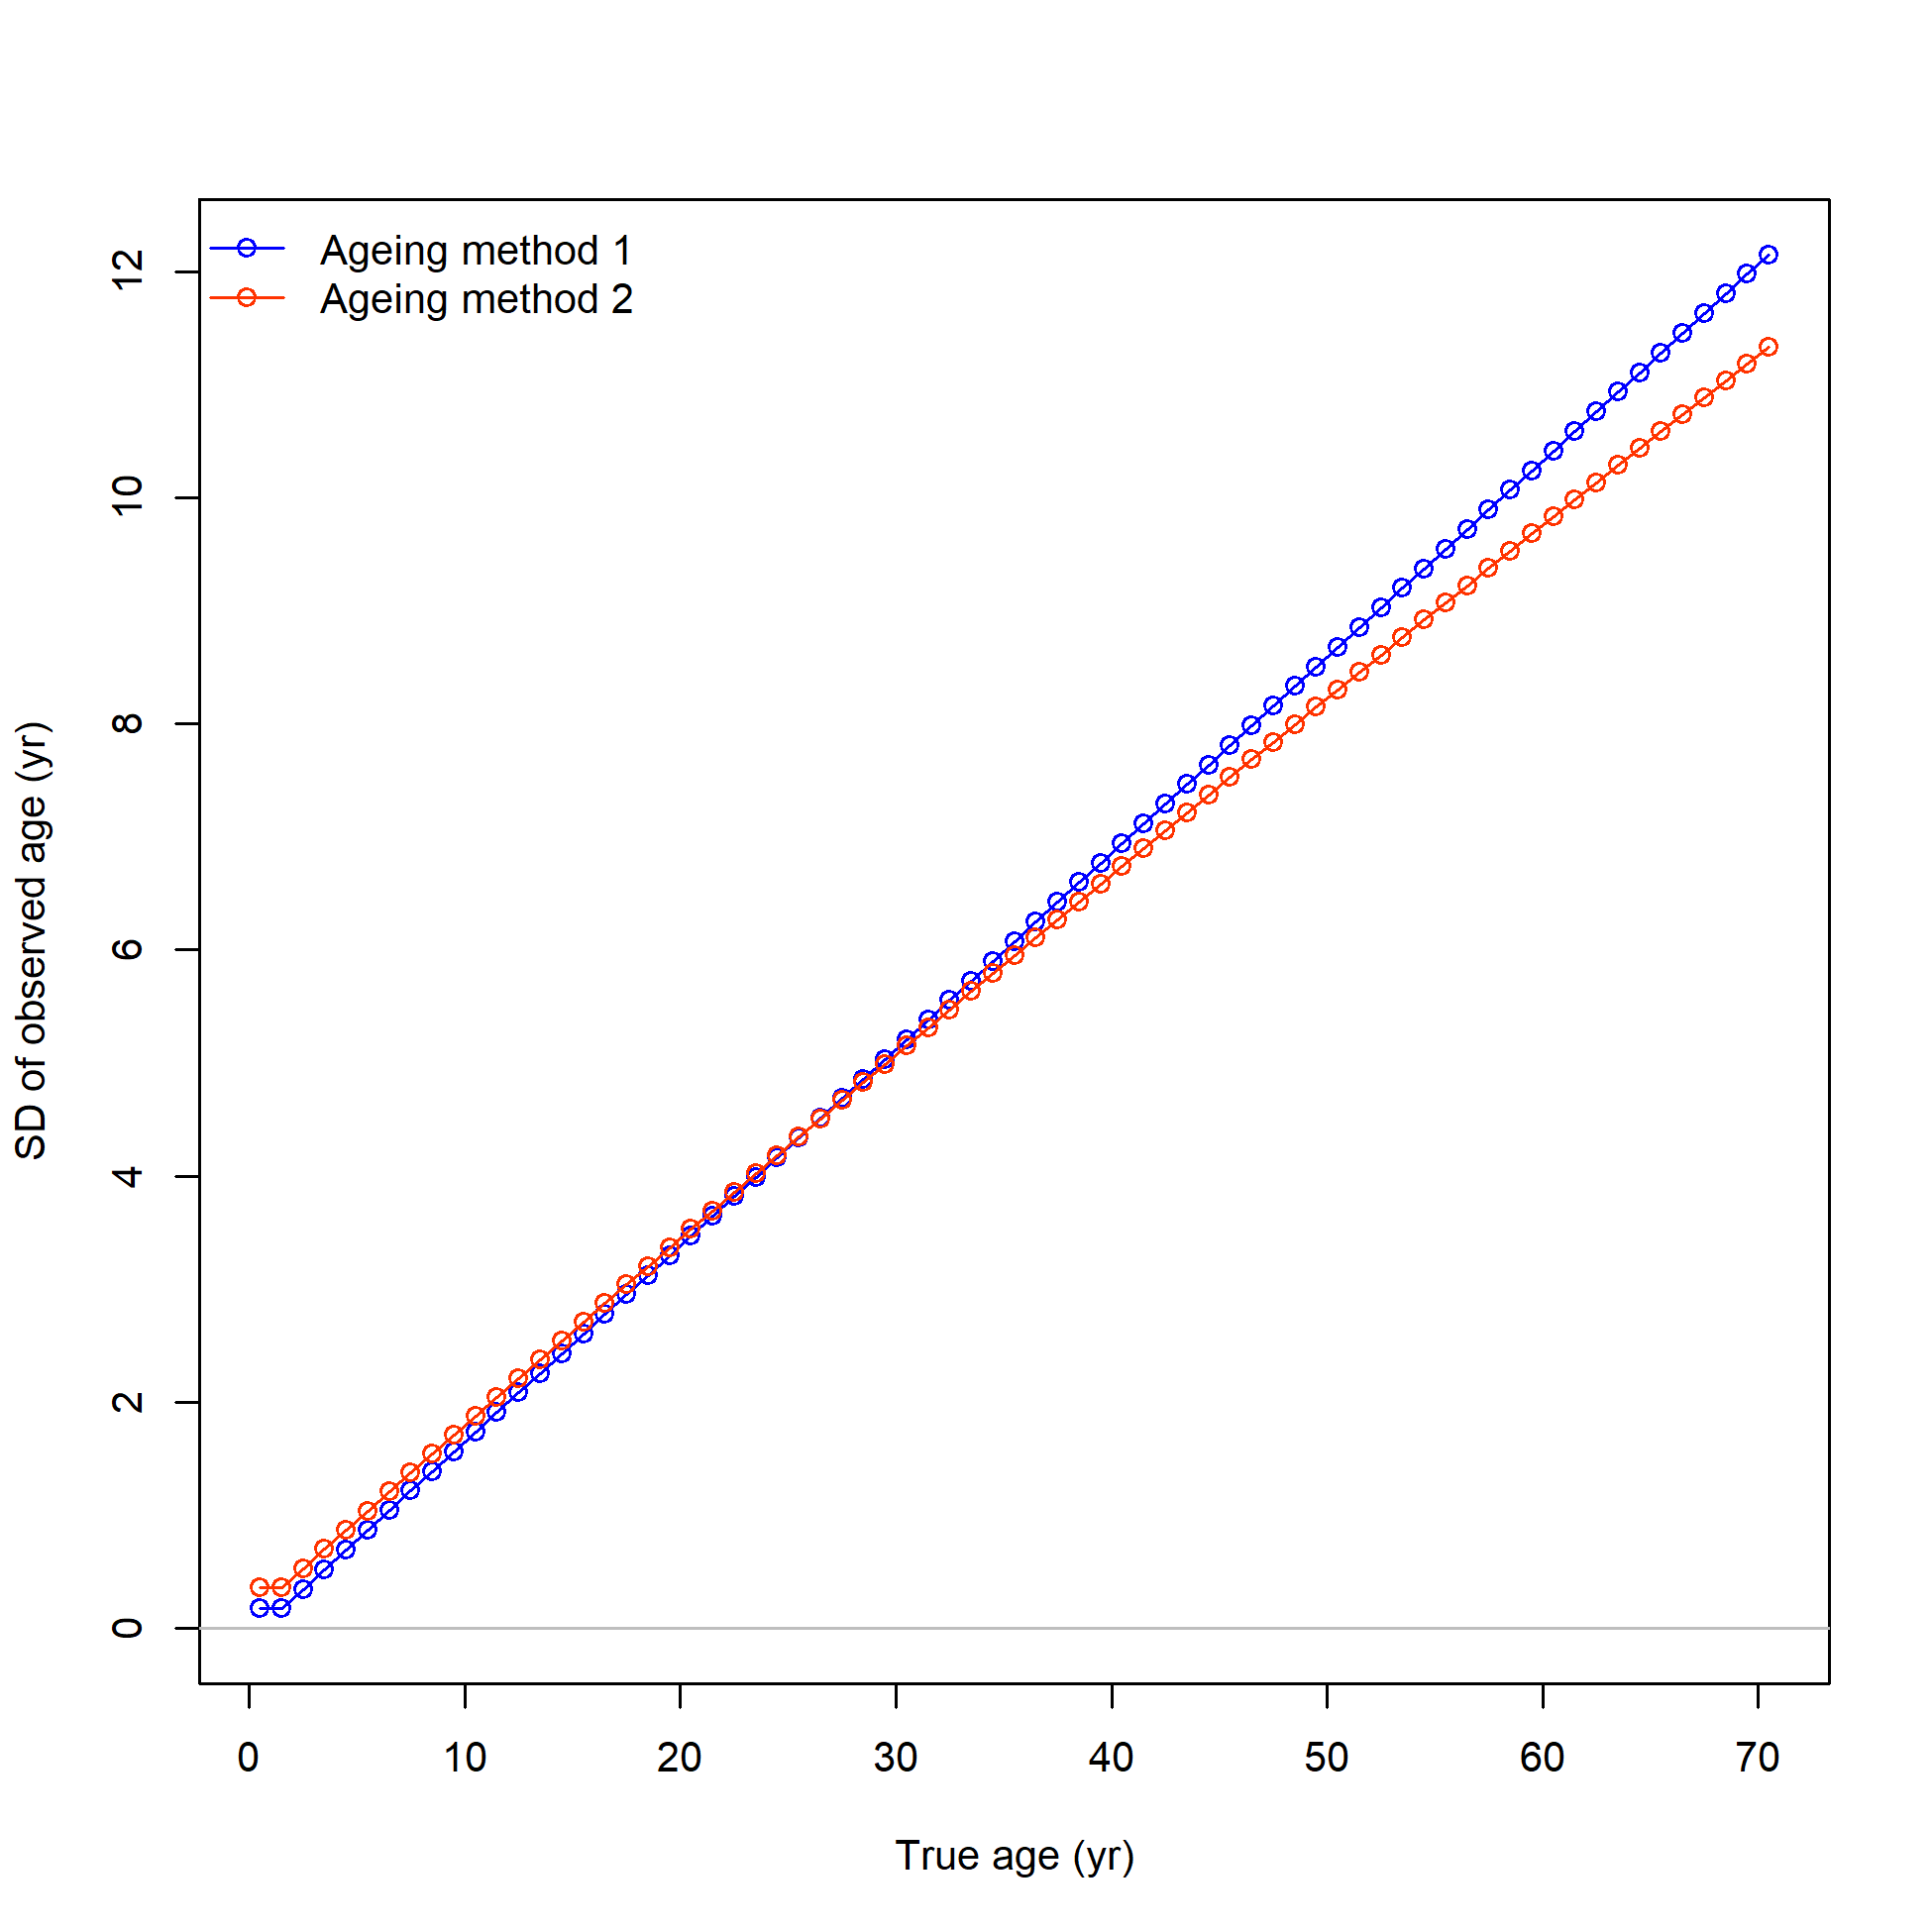
\includegraphics[width=1\linewidth,height=\textheight,keepaspectratio,alt={'Line plot with true age on the x-axis and standard deviation of observed age in years on the y-axis. The standard deviation for ageing error assumed in the model increases linear with age with standard deviation near zero at age 0 and 12 at maximum age of 70.'}]{figures/numbers5_ageerrorSD.png}

}

\caption{\label{fig-ageing-error}Comparison of ageing imprecision,
standard deviation by observed age, used in the base model (blue line -
Ageing method 1) and from the 2019 model (red line - Ageing method 2).}

\end{figure}%

\begin{figure}[H]

\centering{

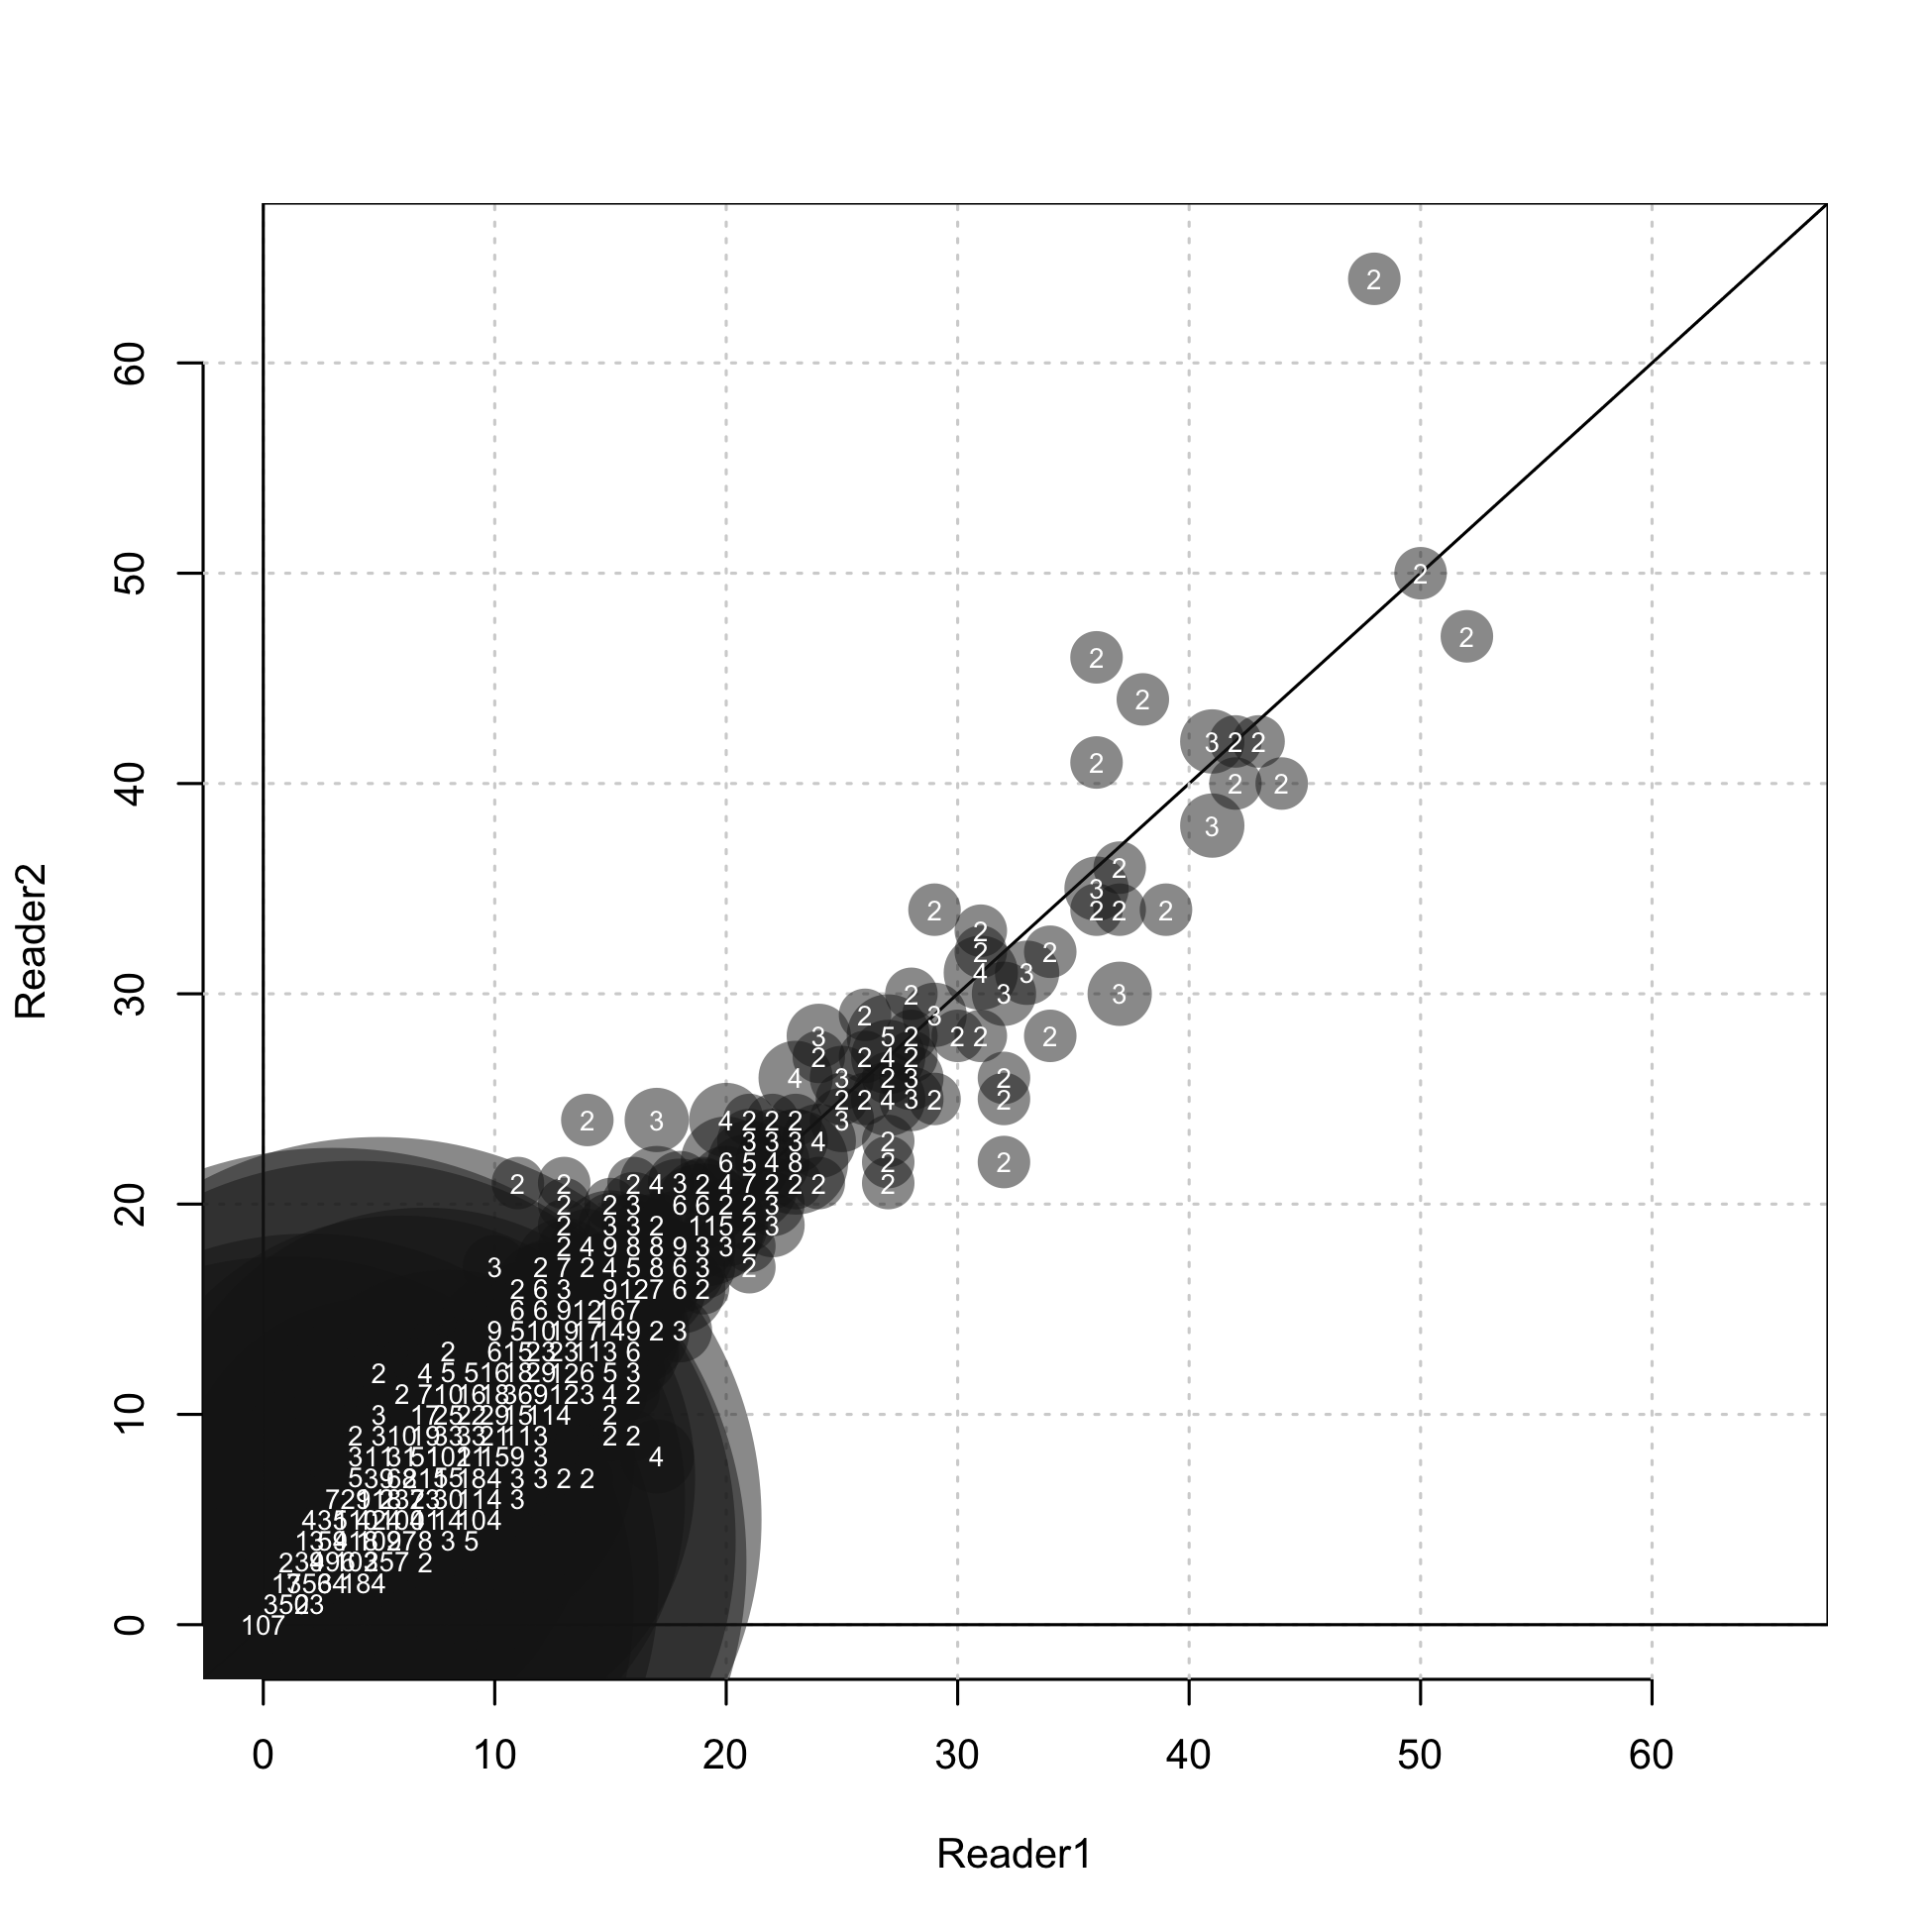
\includegraphics[width=1\linewidth,height=\textheight,keepaspectratio,alt={'Plot of the reader corrispondance for double reads with the read age of reader 1 on the x-axis and the read age of reader 2 on the y-axis. The number of age read pairs are shown in circles with larger circles for larger pair reads.  The age reads by each reader approximately follow the one to one line indicating no bias between readers.'}]{figures/Sablefish-DataSet-1-Reader1VsReader2.png}

}

\caption{\label{fig-age-reader}Comparison of age reads between reader 1
and reader 2 where reader 1 was assumed to be unbiased. The size of the
bubbles is based on the number of age read groups between readers with
larger bubbles for higher age read combinations.}

\end{figure}%

\subsection{Model Bridging}\label{model-bridging}

\begin{figure}[H]

\centering{

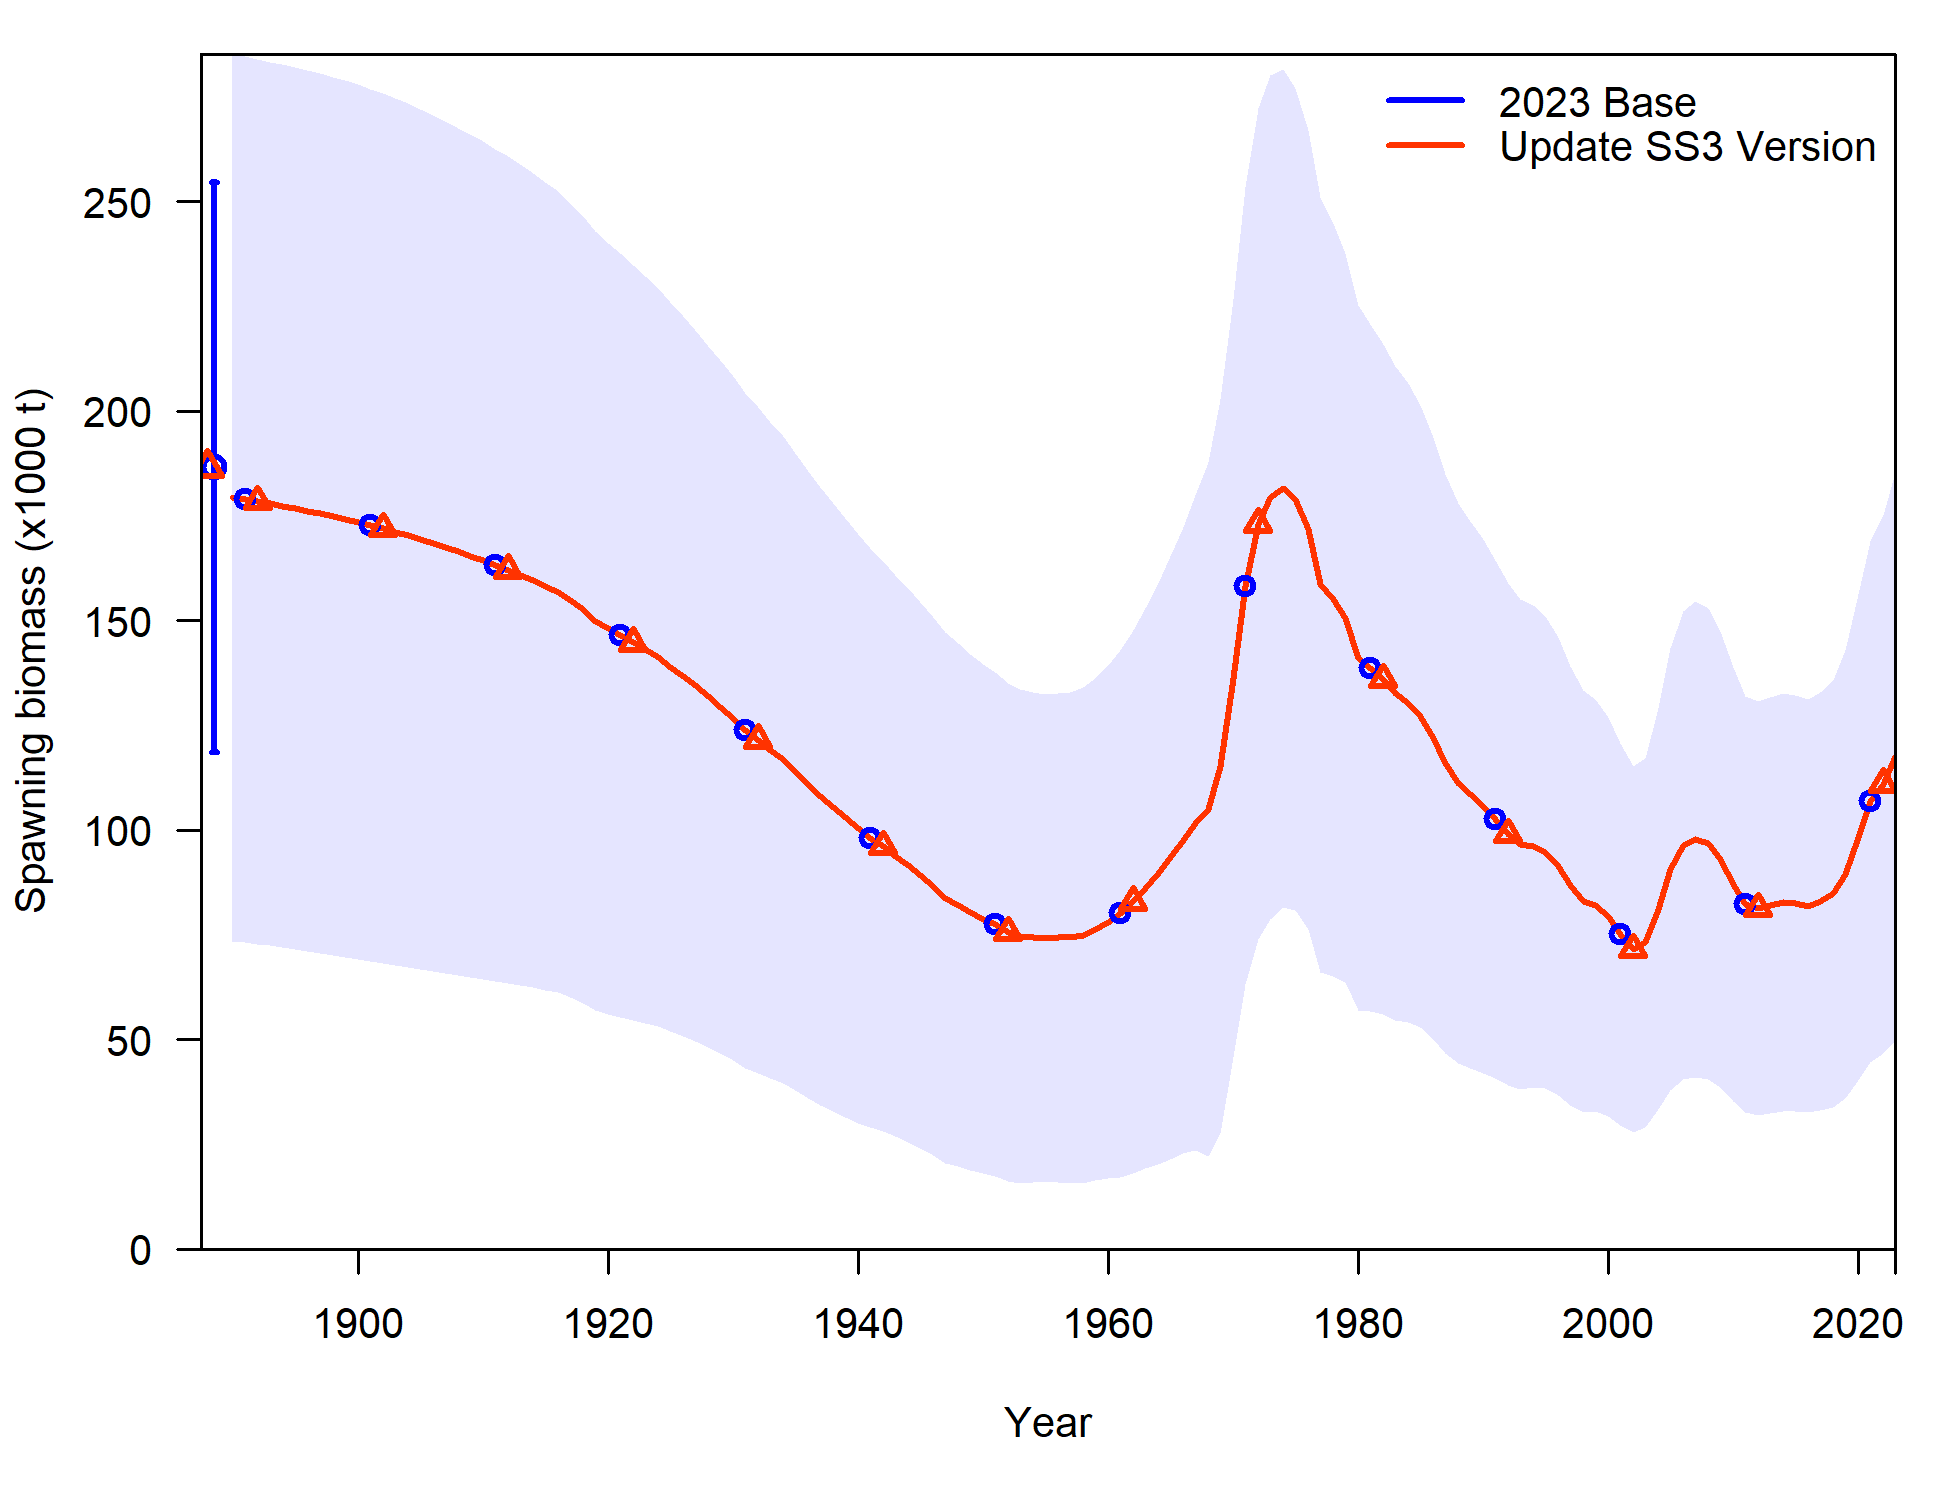
\includegraphics[width=1\linewidth,height=\textheight,keepaspectratio,alt={'Line plot with year on the x-axis and spawning output on the y-axis.  The estimates of spawning output between the two versions of Stock Synthesis are identical for all years.'}]{figures/0_bridging_compare2_spawnbio_uncertainty.png}

}

\caption{\label{fig-ss3-version}Comparison of estimated spawning output
(e.g., spawning biomass) between Stock Synthesis executable versions.}

\end{figure}%

\pagebreak

\begin{figure}[H]

\centering{

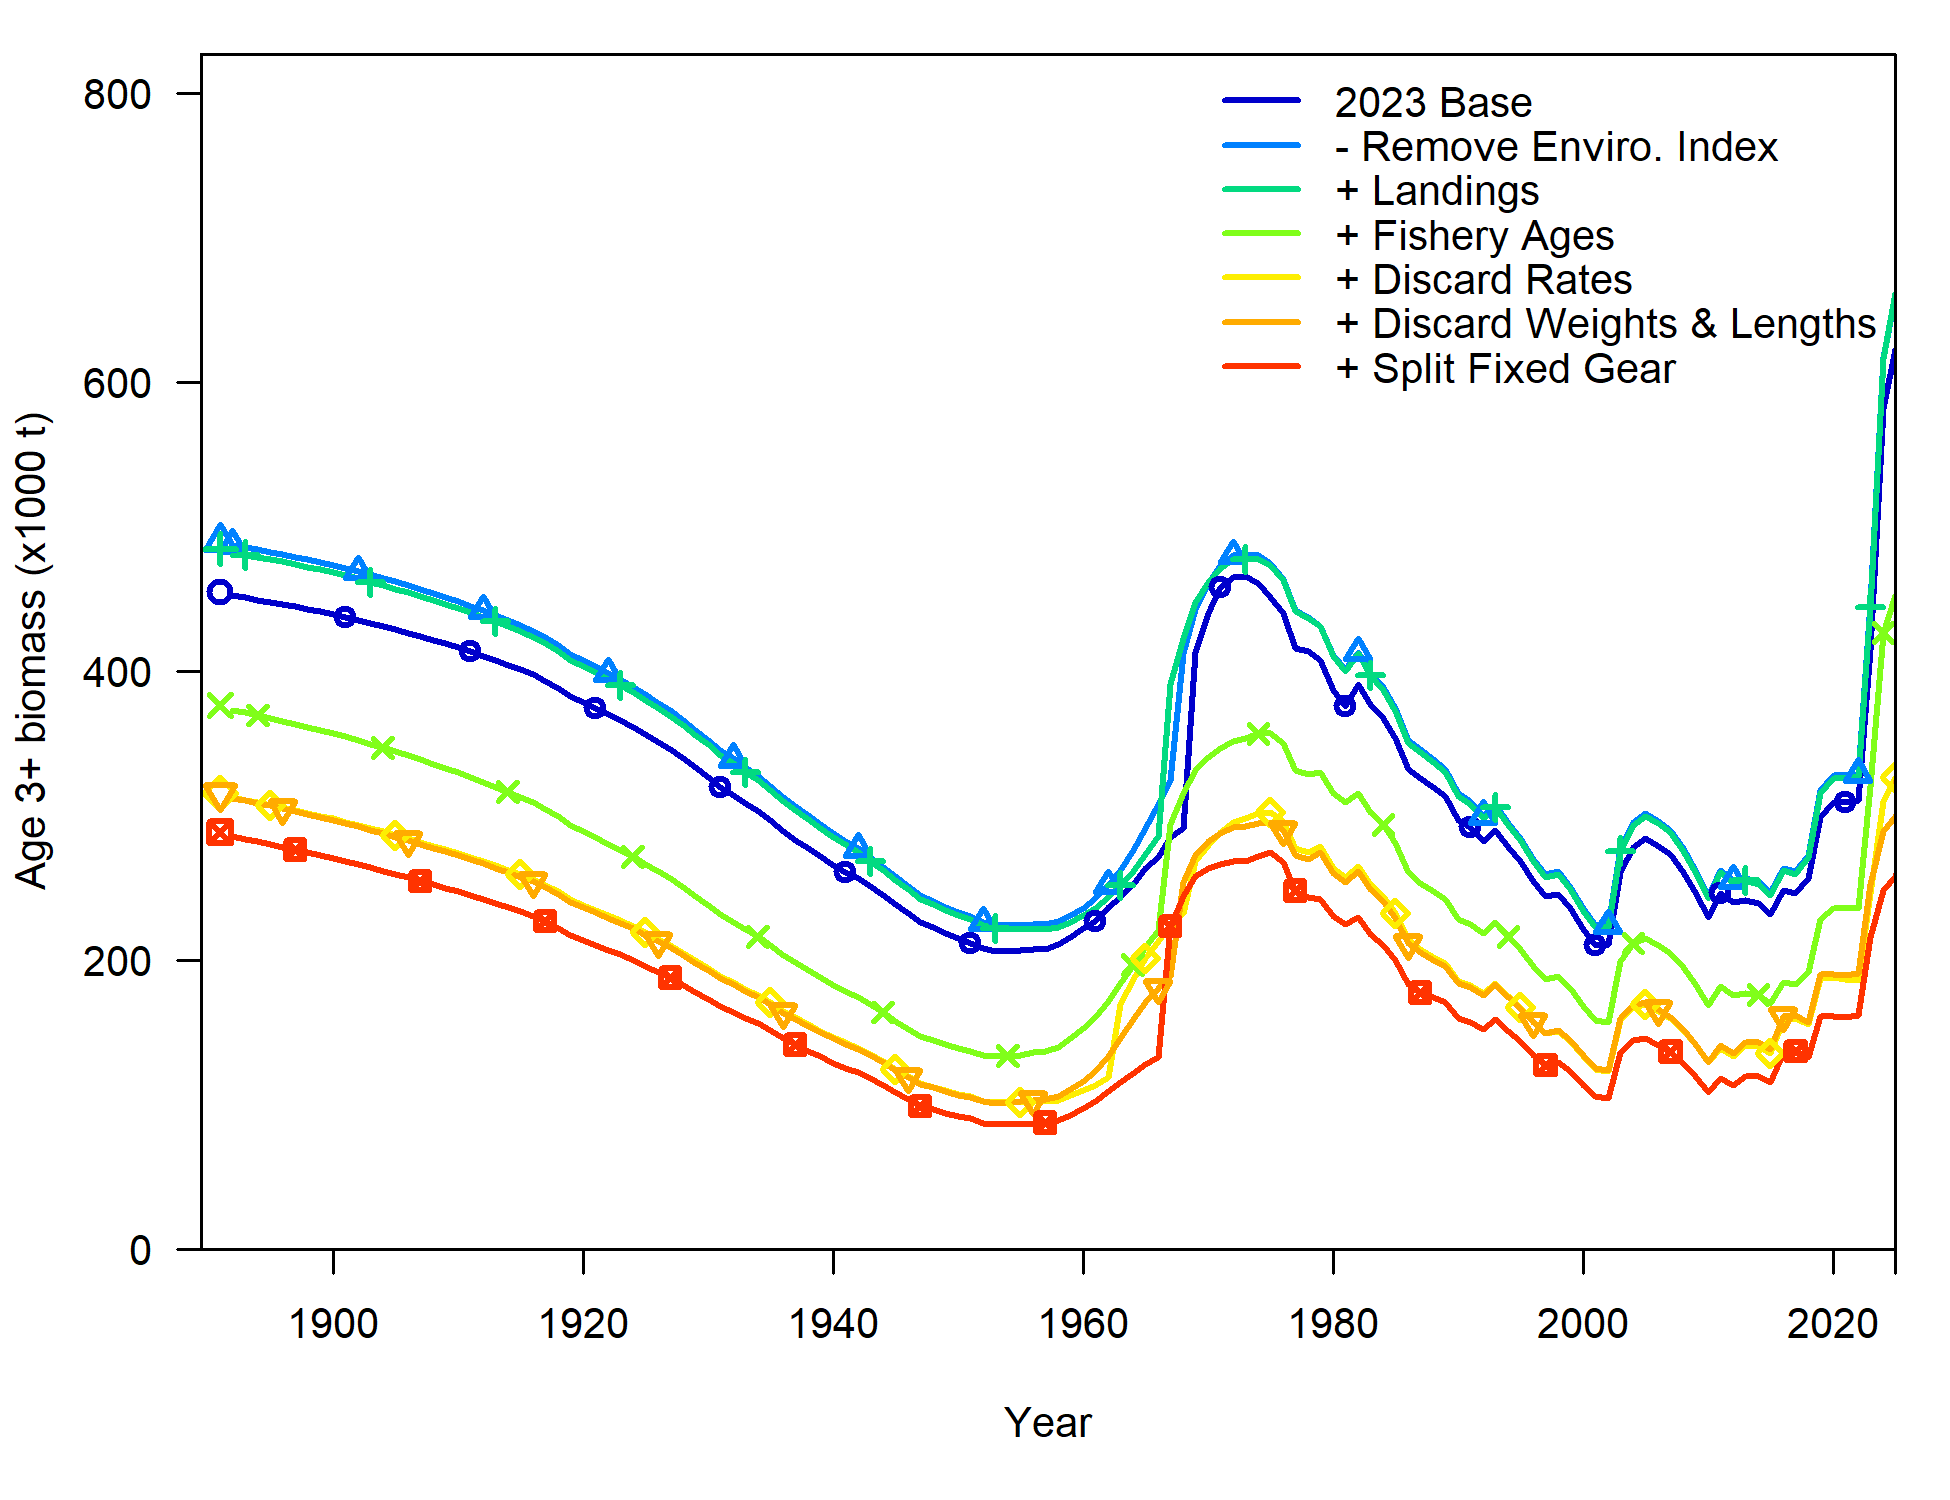
\includegraphics[width=1\linewidth,height=\textheight,keepaspectratio,alt={'Line plot with year on the x-axis and age 3 plus biomass on the y-axis. As new data and reprocessed data are added to the 2023 model the estimates of age 3 plus biomass decreases across all years compared to the estimates from the 2023 model. The section 3.3.3 model changes from the last assessment describes in detail the changes to estimates.'}]{figures/1_data_bridging_compare18_smrybio.png}

}

\caption{\label{fig-data-bridge-summary-1}Comparison of estimated
summary biomass for ages 3+ when adding new data.}

\end{figure}%

\begin{figure}[H]

\centering{

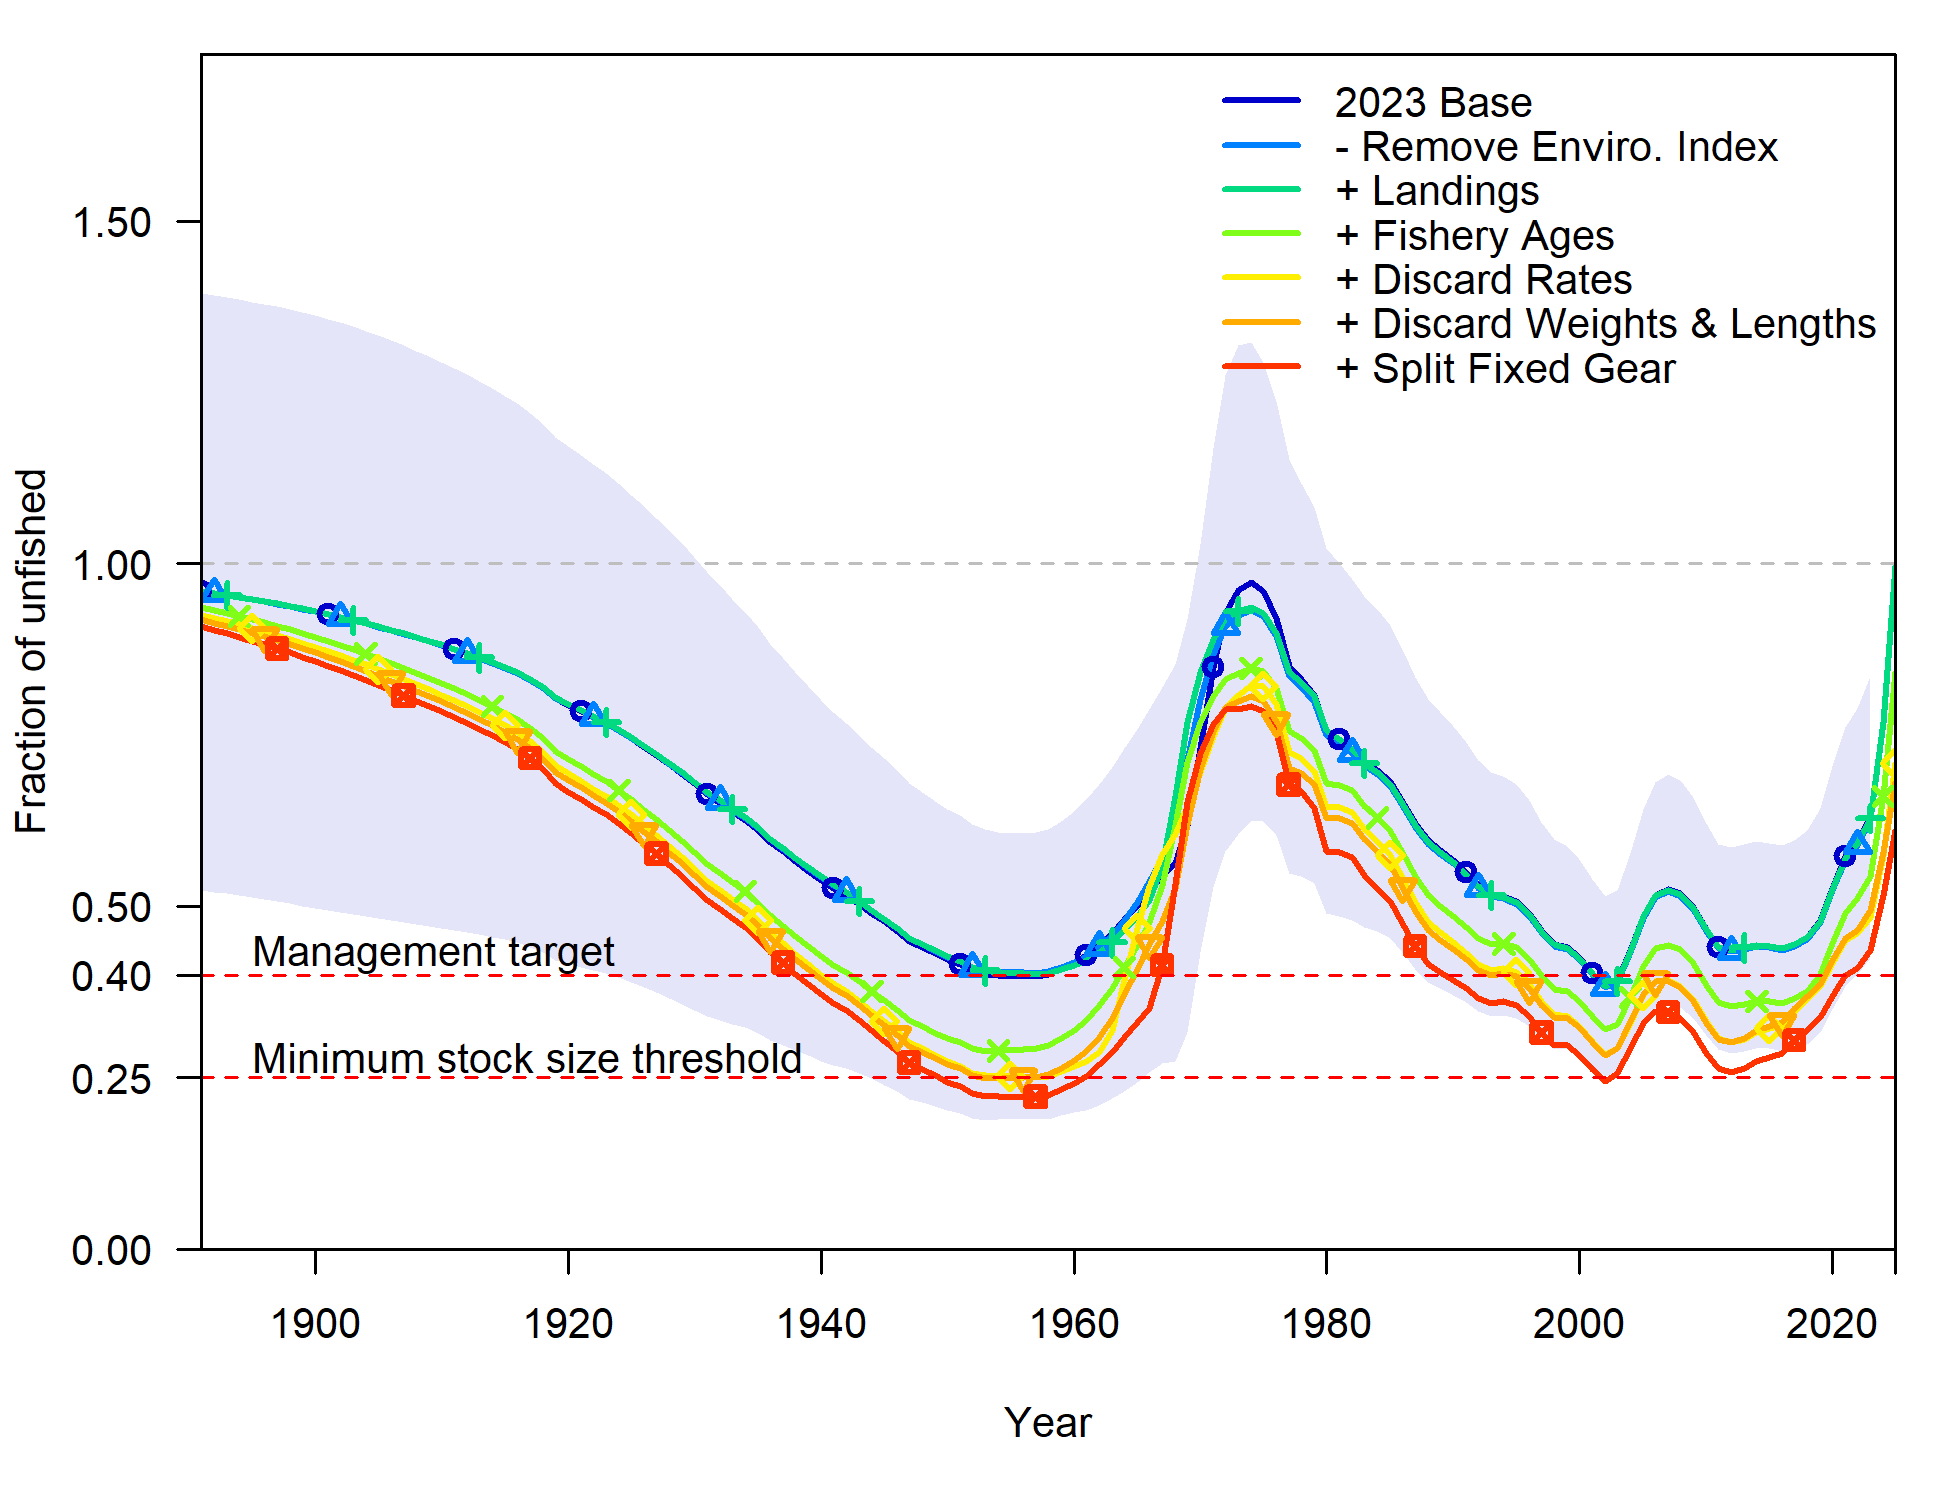
\includegraphics[width=1\linewidth,height=\textheight,keepaspectratio,alt={'Line plot with year on the x-axis and fraction of unfished on the y-axis. As new data and reprocessed data are added to the 2023 model the estimates of fraction of unfished decreases across all years compared to the estimates from the 2023 model. The section 3.3.3 model changes from the last assessment describes in detail the changes to estimates.'}]{figures/1_data_bridging_compare4_Bratio_uncertainty.png}

}

\caption{\label{fig-data-bridge-depl-1}Comparison of estimated fraction
unfished (i.e., stock status) when adding new data.}

\end{figure}%

\begin{figure}[H]

\centering{

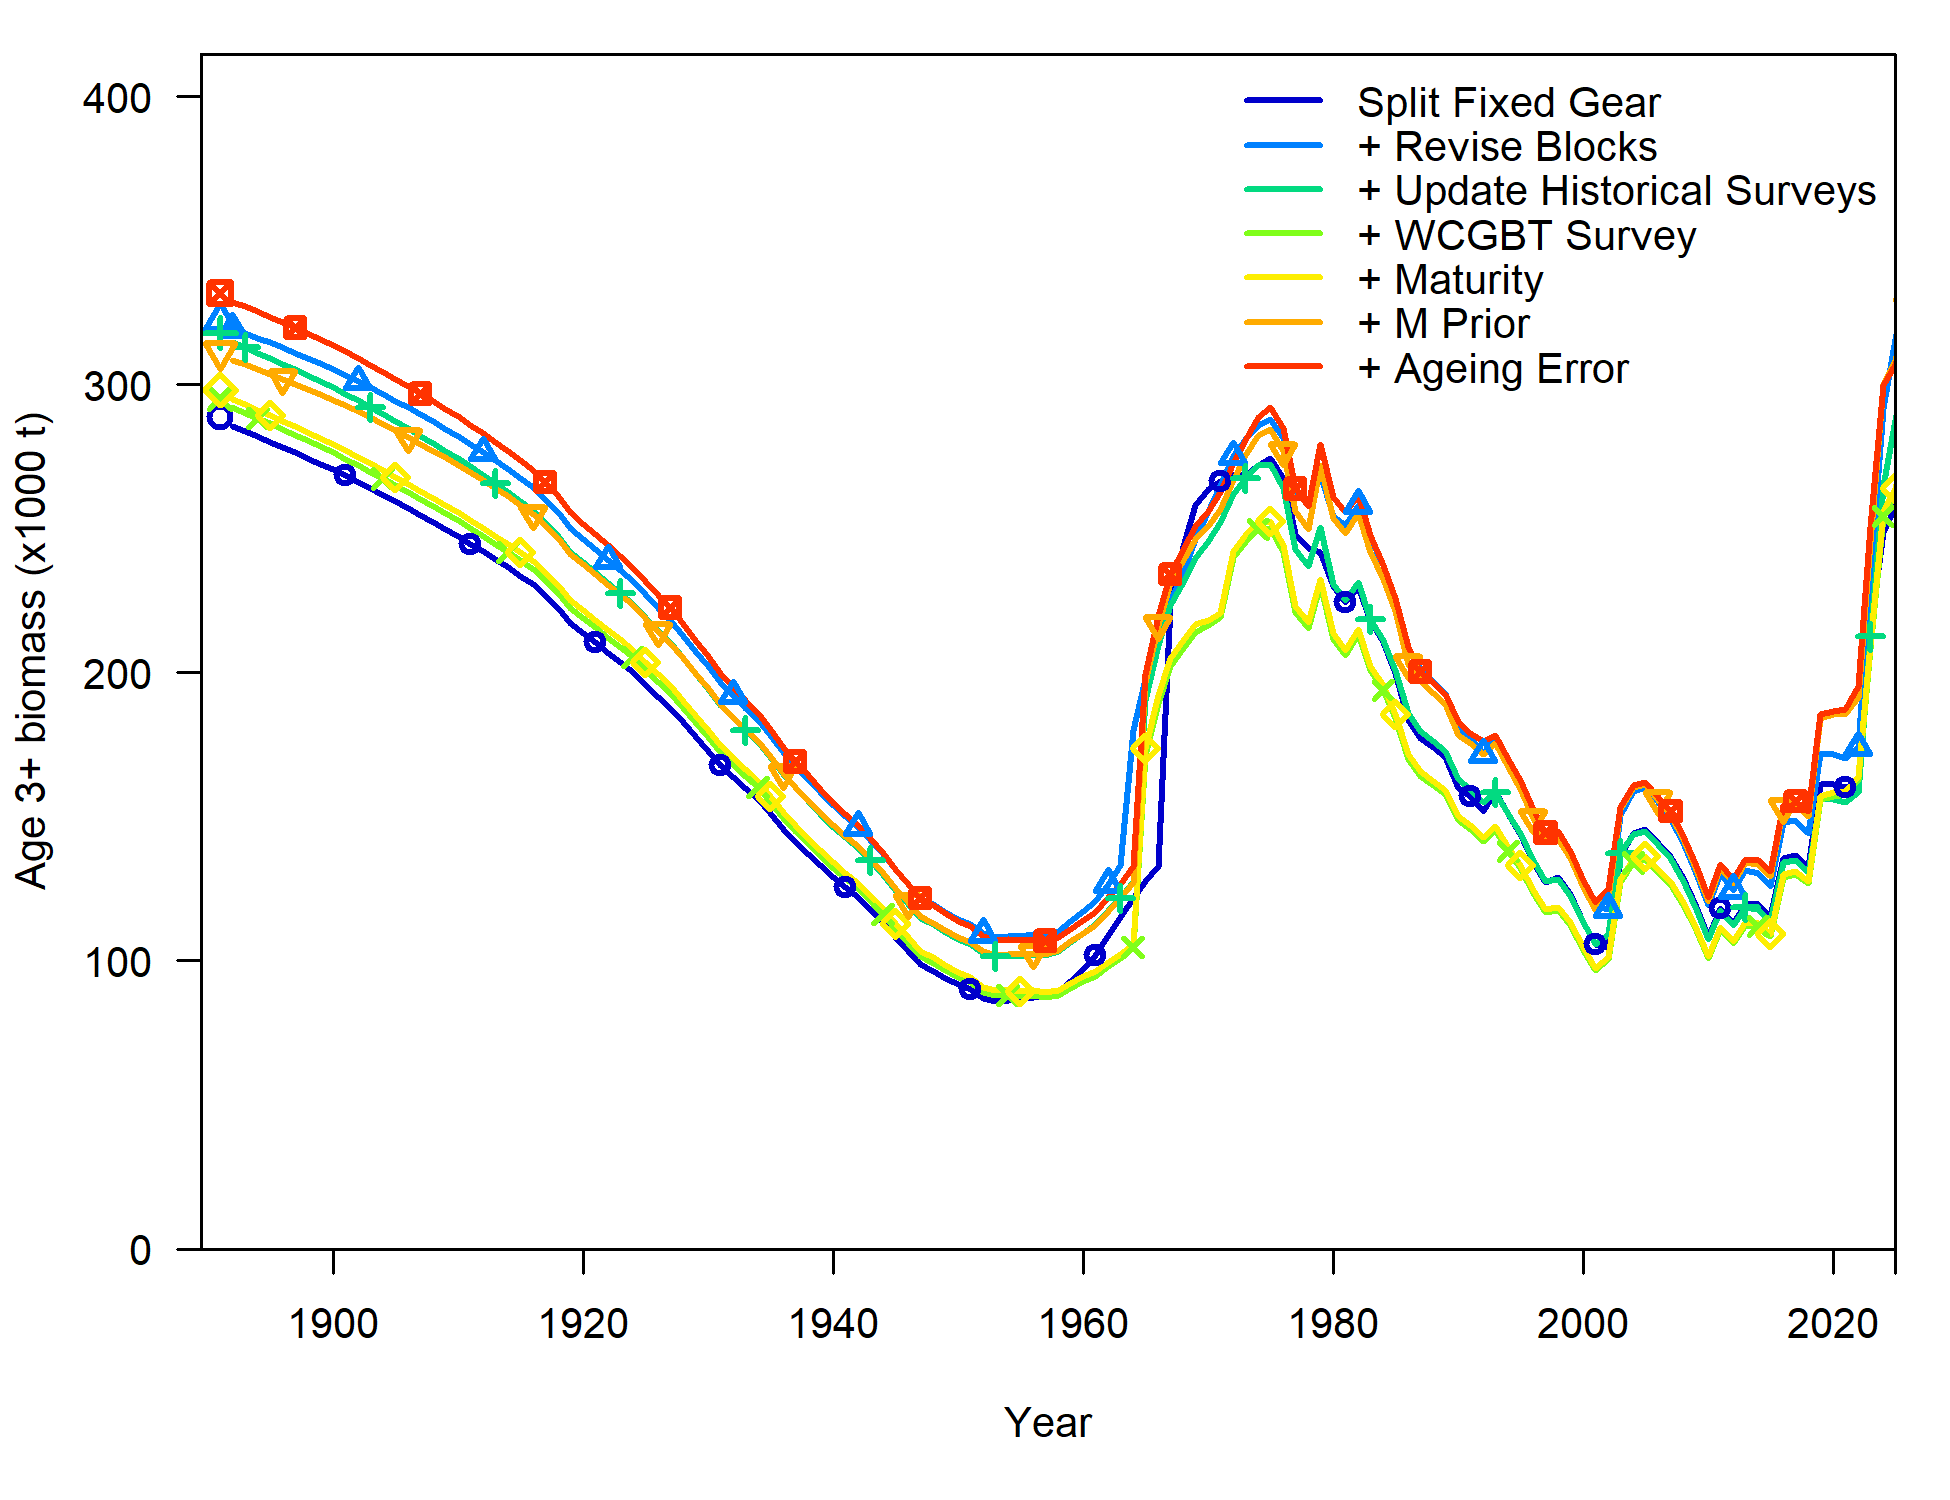
\includegraphics[width=1\linewidth,height=\textheight,keepaspectratio,alt={'Line plot with year on the x-axis and age 3 plus biomass on the y-axis. As new and reprocessed data and model structure and parameter assumptions are revised from the 2023 model the estimates of age 3 plus biomass slightly increases across all years compared to data bridging. The section 3.3.3 model changes from the last assessment describes in detail the changes to estimates.'}]{figures/2_data_bridging_compare18_smrybio.png}

}

\caption{\label{fig-data-bridge-summary-2}Comparison of estimated
summary biomass for ages 3+ when adding new data.}

\end{figure}%

\begin{figure}[H]

\centering{

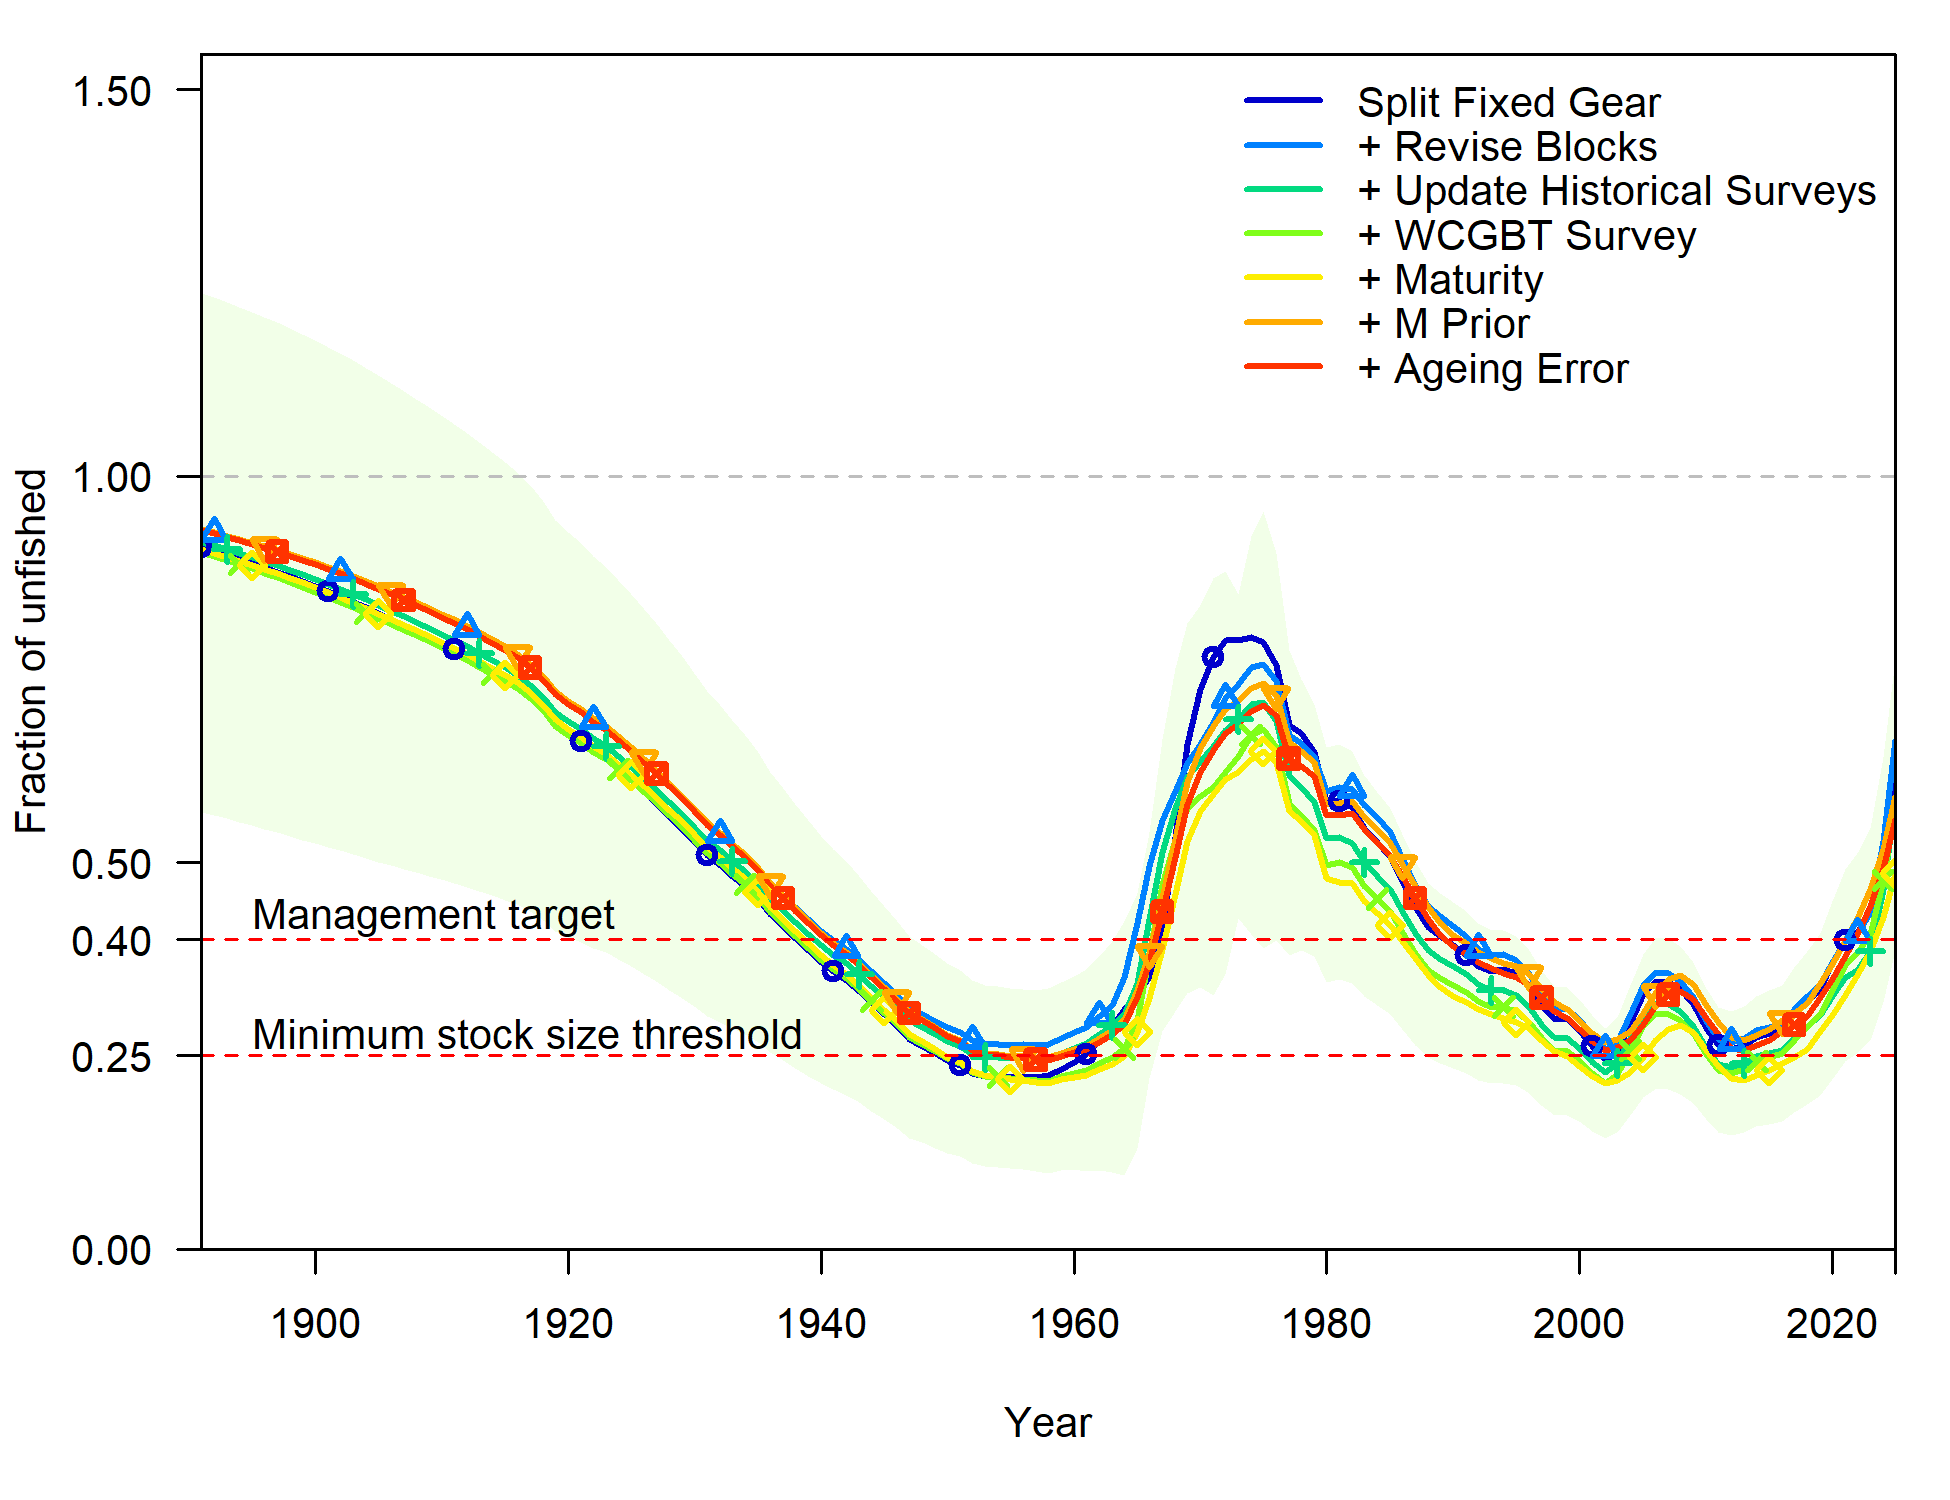
\includegraphics[width=1\linewidth,height=\textheight,keepaspectratio,alt={'Line plot with year on the x-axis and fraction of unfished on the y-axis. As new and reprocessed data and model structure and parameter assumptions are revised from the 2023 model the estimates of fraction of unfished are similar for mos years in the time series but the final fraction of unfished slightly decreases in 2024 and 2025 compared to data bridging. The section 3.3.3 model changes from the last assessment describes in detail the changes to estimates.'}]{figures/2_data_bridging_compare4_Bratio_uncertainty.png}

}

\caption{\label{fig-data-bridge-depl-2}Comparison of estimated fraction
unfished (i.e., stock status) when adding new data.}

\end{figure}%

\begin{figure}[H]

\centering{

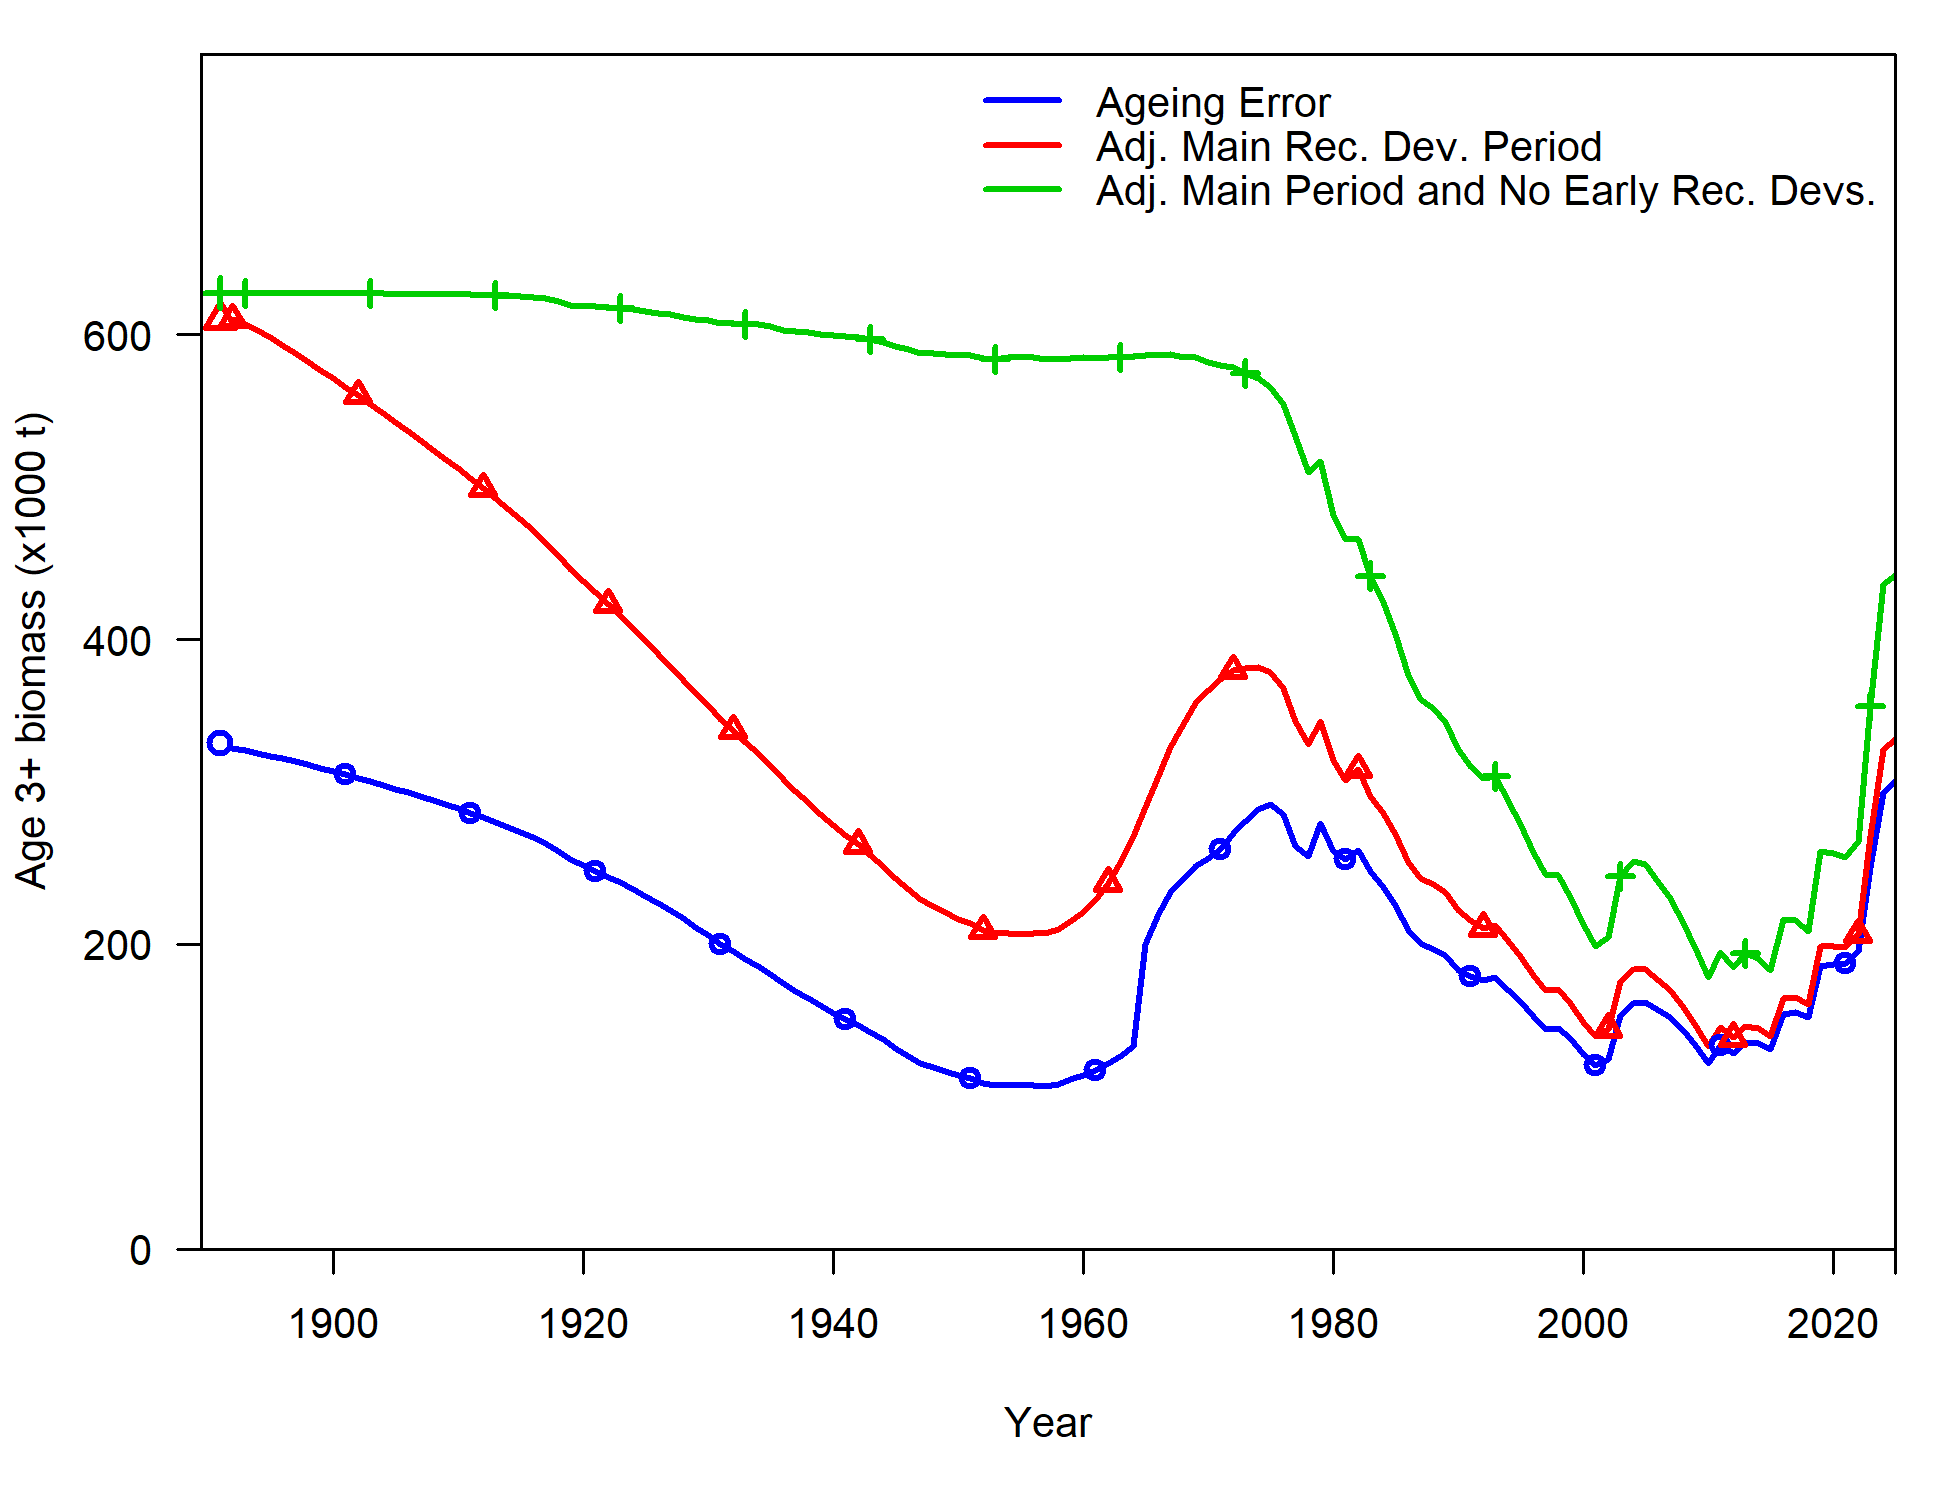
\includegraphics[width=1\linewidth,height=\textheight,keepaspectratio,alt={'Line plot with year on the x-axis and age 3 plus biomass on the y-axis. Changing the main period for the estimation of recruitment deviation to run from 1975 through 2023 increases the estimate of unfished age 3 plus biomass to approximately 600,000 metric tons compared to the previous model that assumed a main period of 1925 through 2023 estimate of approximately 350,000 metric tons. The estimated age 3 plus biomass at the end of the time series were similar around 400,000 metric tons. The next bridging run that did not estimate early recruitment deviations from 1892 to 1974 estimated similar age 3 plus biomass at the start of the time series to the model with main deviations from 1975 to 2023, but the model with no early deviations estimated higher age 3 plus biomass at the end of the time series of greater than 450,000 metric tons. Section 3.3.3 model changes from the last assessment describes in detail the changes to estimates.'}]{figures/3_structure_compare18_smrybio.png}

}

\caption{\label{fig-structure-bridge-summary-3}Comparison of estimated
summary biomass for ages 3+ when the estimation of annual recruitment
deviations is revised.}

\end{figure}%

\begin{figure}[H]

\centering{

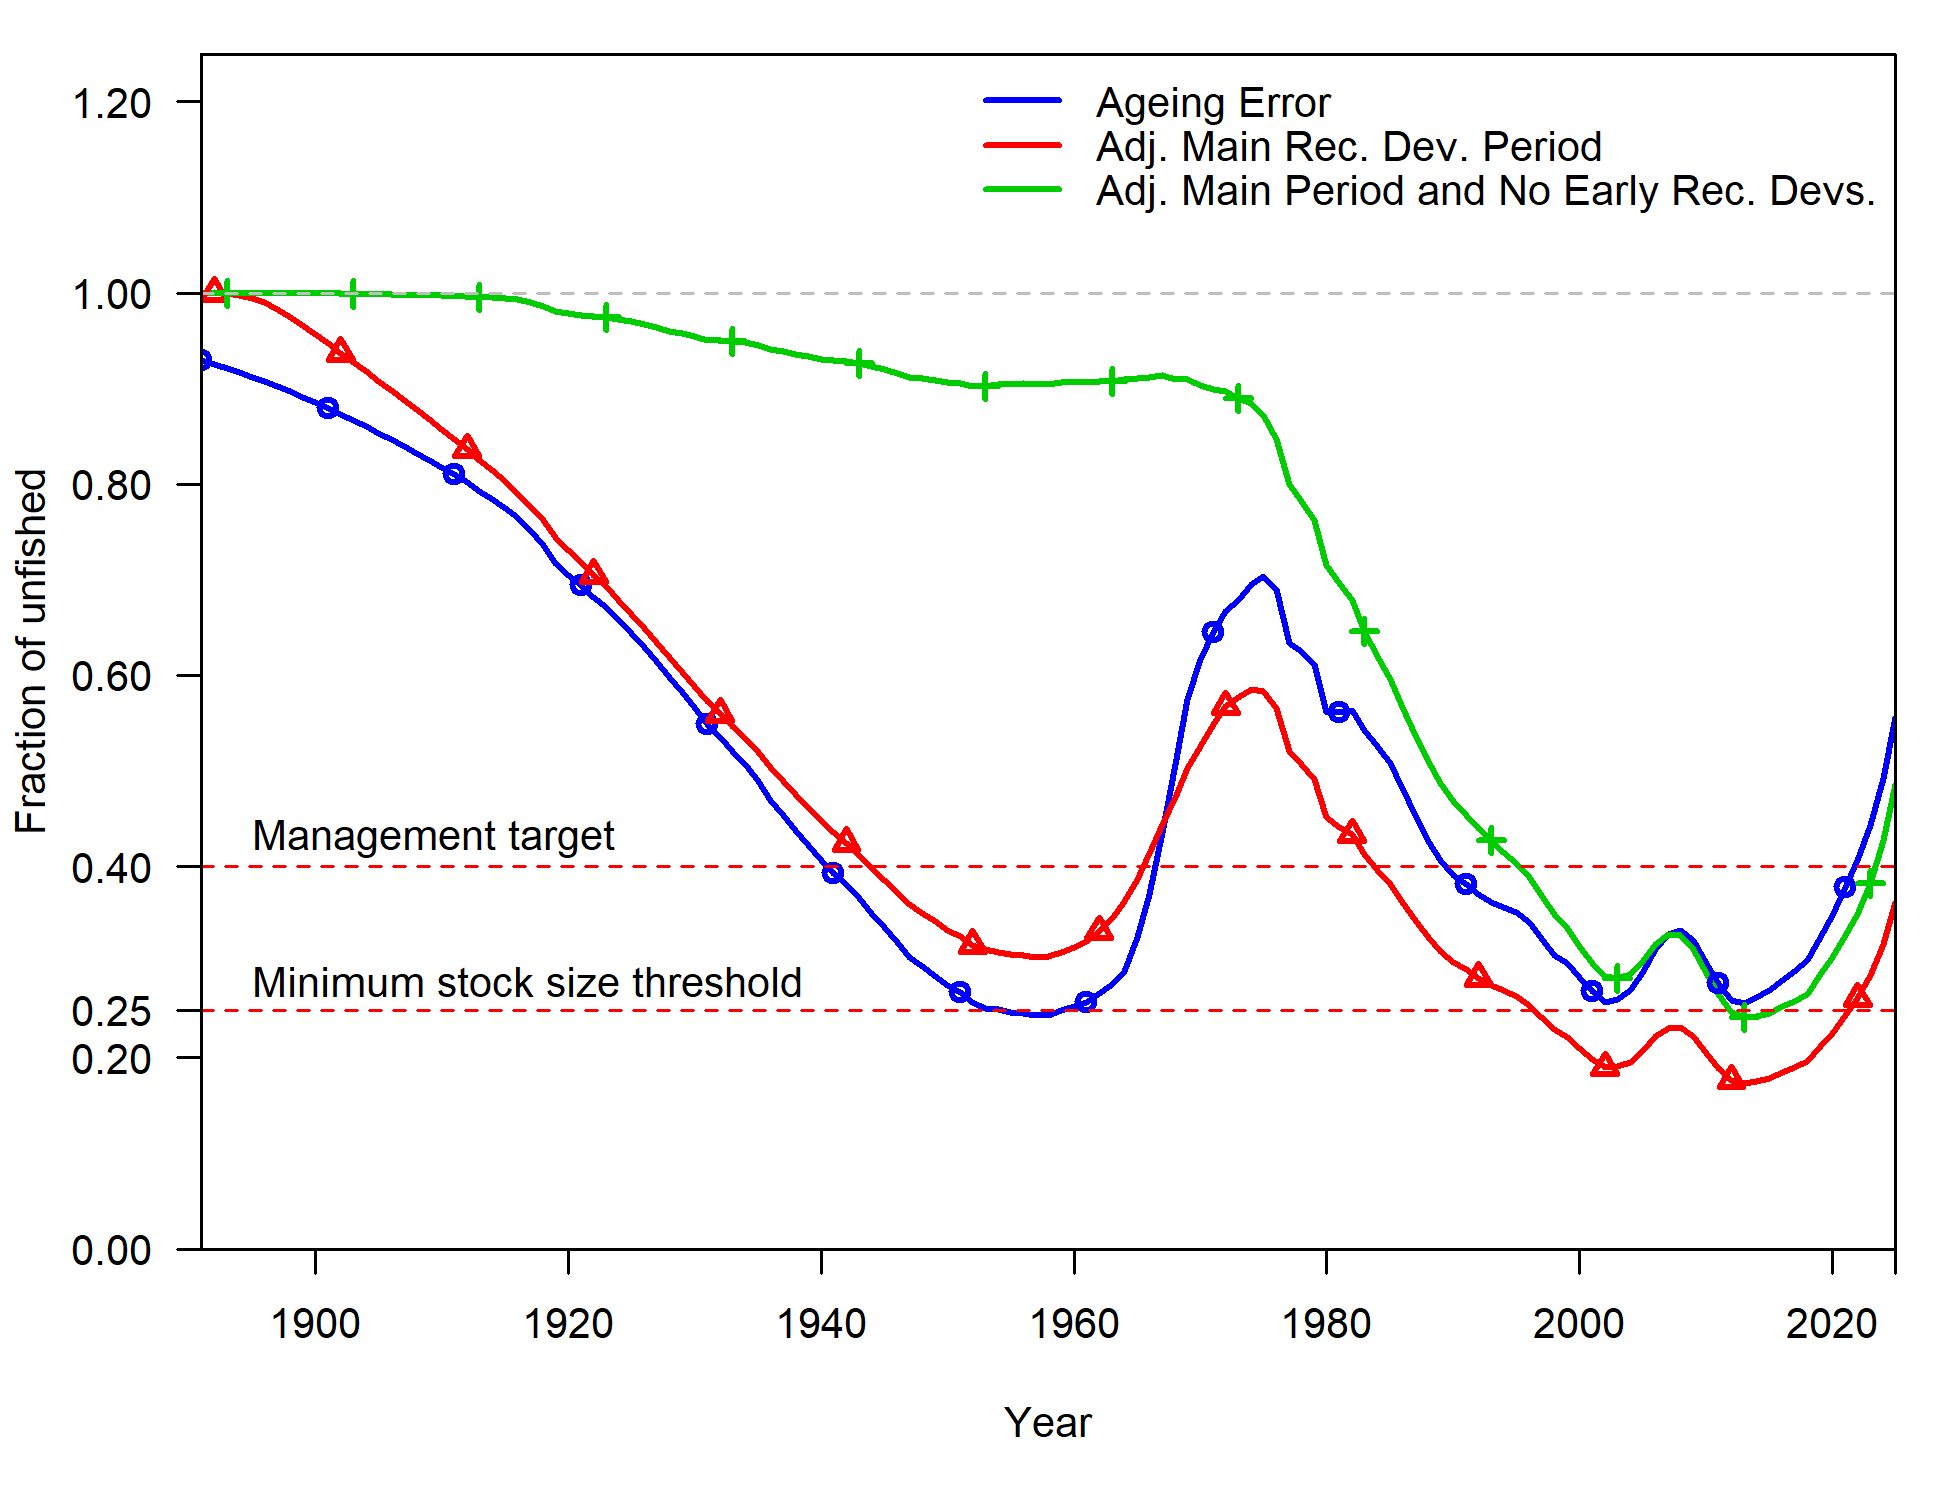
\includegraphics[width=1\linewidth,height=\textheight,keepaspectratio,alt={'Line plot with year on the x-axis and fraction unfished on the y-axis. Changing the main period for the estimation of recruitment deviation to run from 1975 through 2023 estimated a more depleted population across th majority of the time sers compared to the previous model that assumed a main period of 1925 through 2023. The estimated fraction of unfished for the shorter main deviation period model was approximately 37 percent compared to 55 percent of the previous model. The next bridging run that did not estimate early recruitment deviations from 1892 to 1974 estimated a less depleted population through 2000 compared to the model with the main deviation period of 1975 through 2023. The final estimate of fraction of unfished was approximately 45 percent in 2025. Section 3.3.3 model changes from the last assessment describes in detail the changes to estimates.'}]{figures/3_structure_compare3_Bratio.png}

}

\caption{\label{fig-structure-bridge-depl-3}Comparison of estimated
fraction unfished (i.e., stock status) when the estimation of annual
recruitment deviations is revised.}

\end{figure}%

\begin{figure}[H]

\centering{

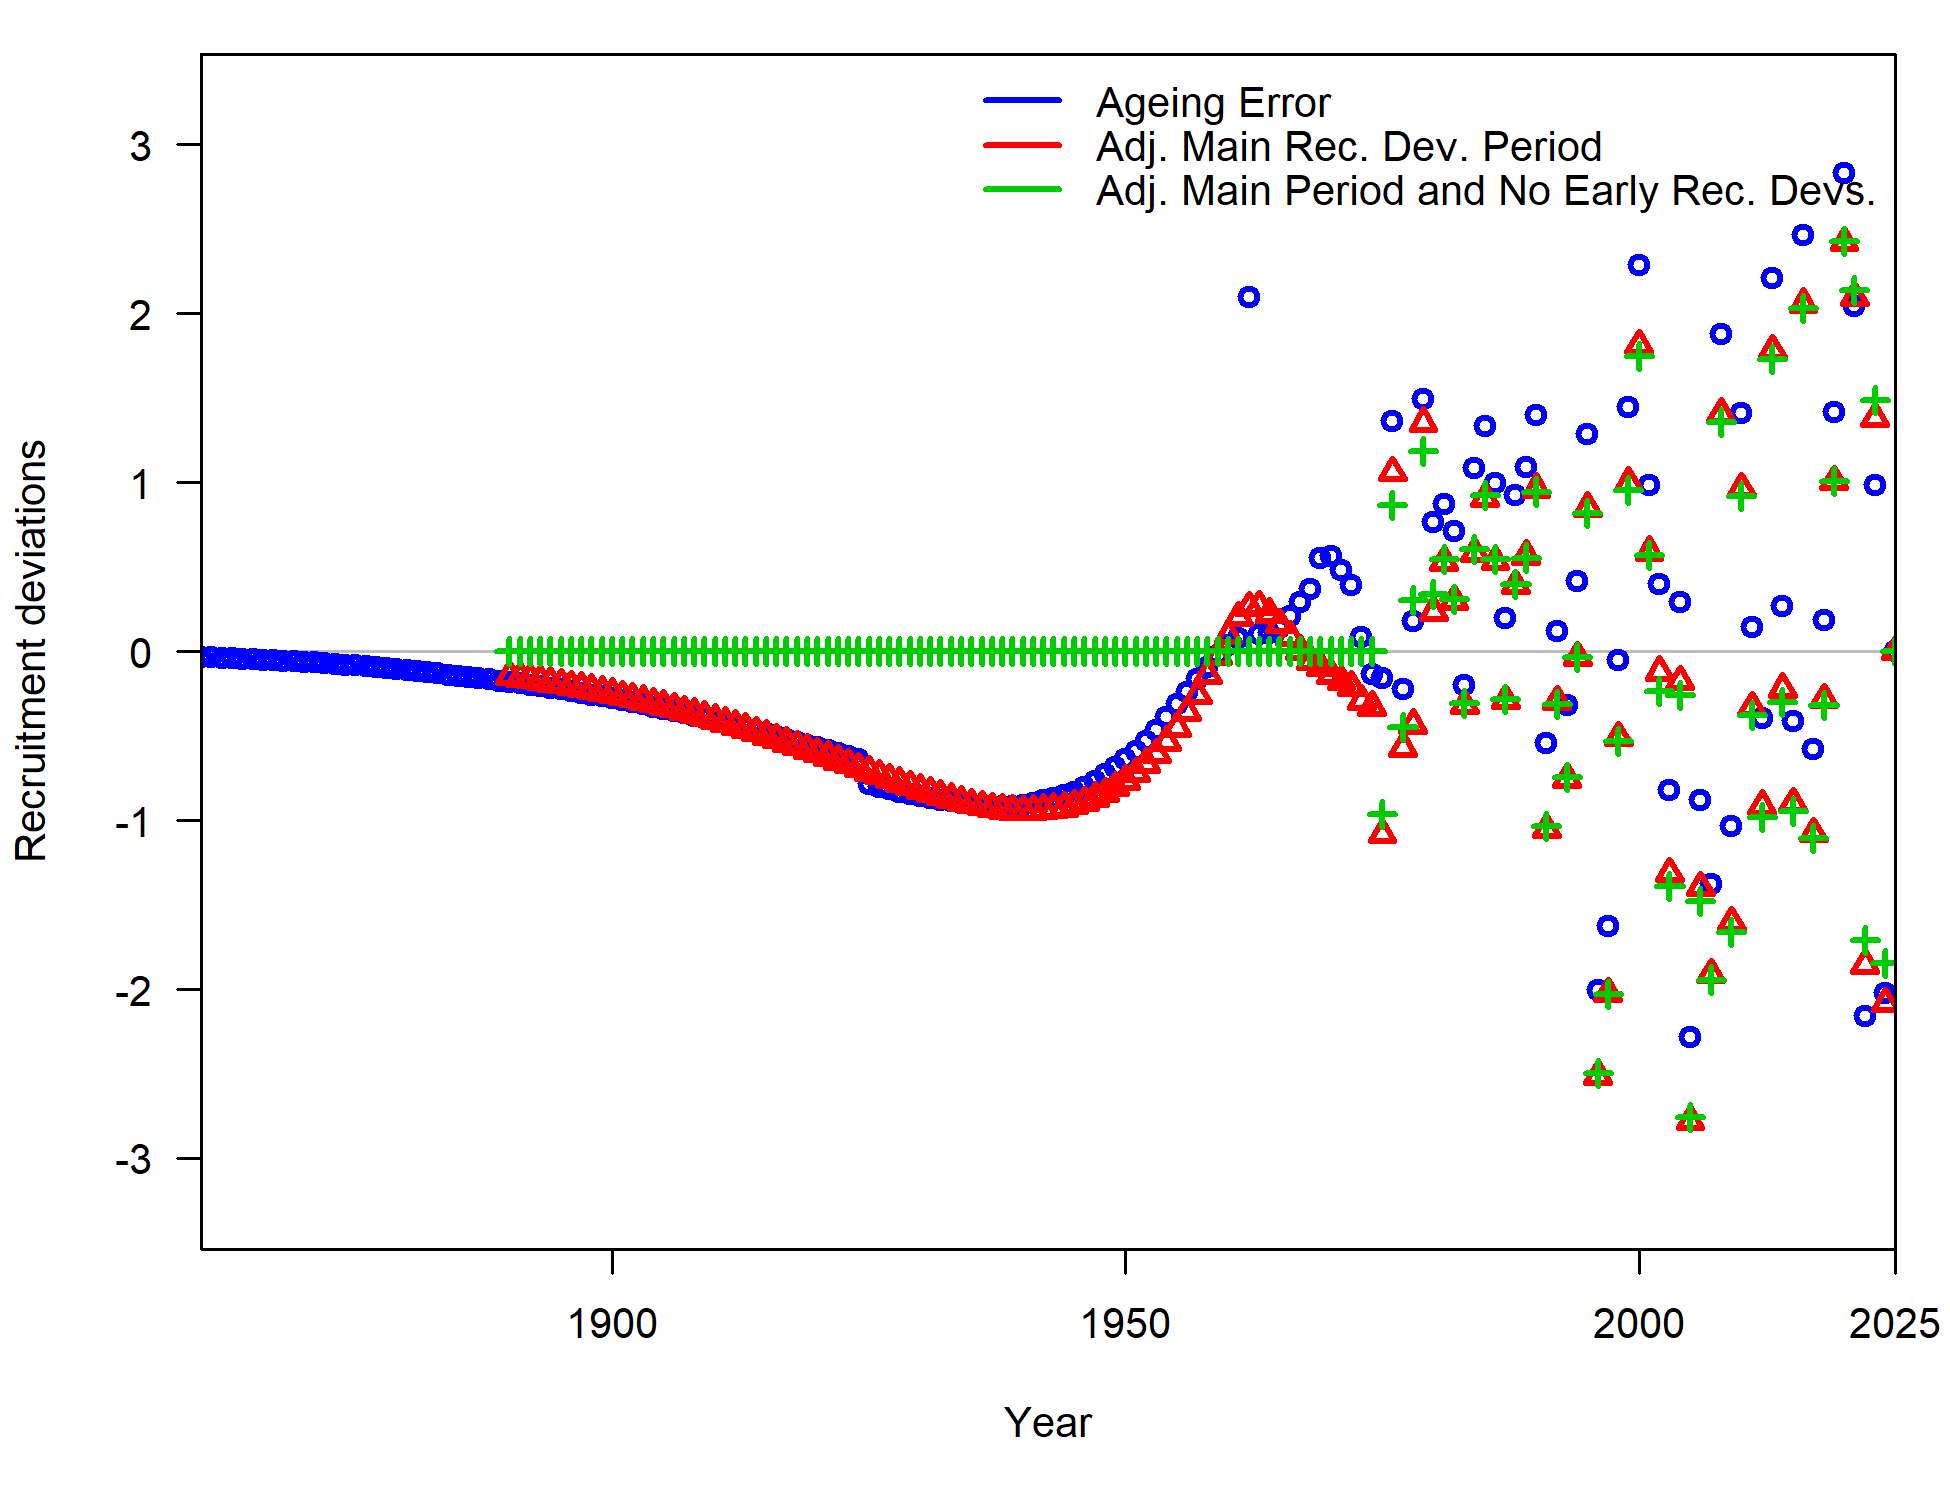
\includegraphics[width=1\linewidth,height=\textheight,keepaspectratio,alt={'Plot with year on the x-axis and recruitment deviations in log-space on the y-axis. The estimates of recruitment deviations for the model with the main period of 1975 through 2023 and the model with no early deviations were generally more positive and negative compared to the model with the main period of 1925 through 2023 with early deviations estimated.'}]{figures/3_structure_compare11_recdevs.png}

}

\caption{\label{fig-structure-bridge-rec-dev-3}Comparison of estimated
annual recruitment deviations when the estimation of annual recruitment
deviations is revised.}

\end{figure}%

\pagebreak

\begin{figure}[H]

\centering{

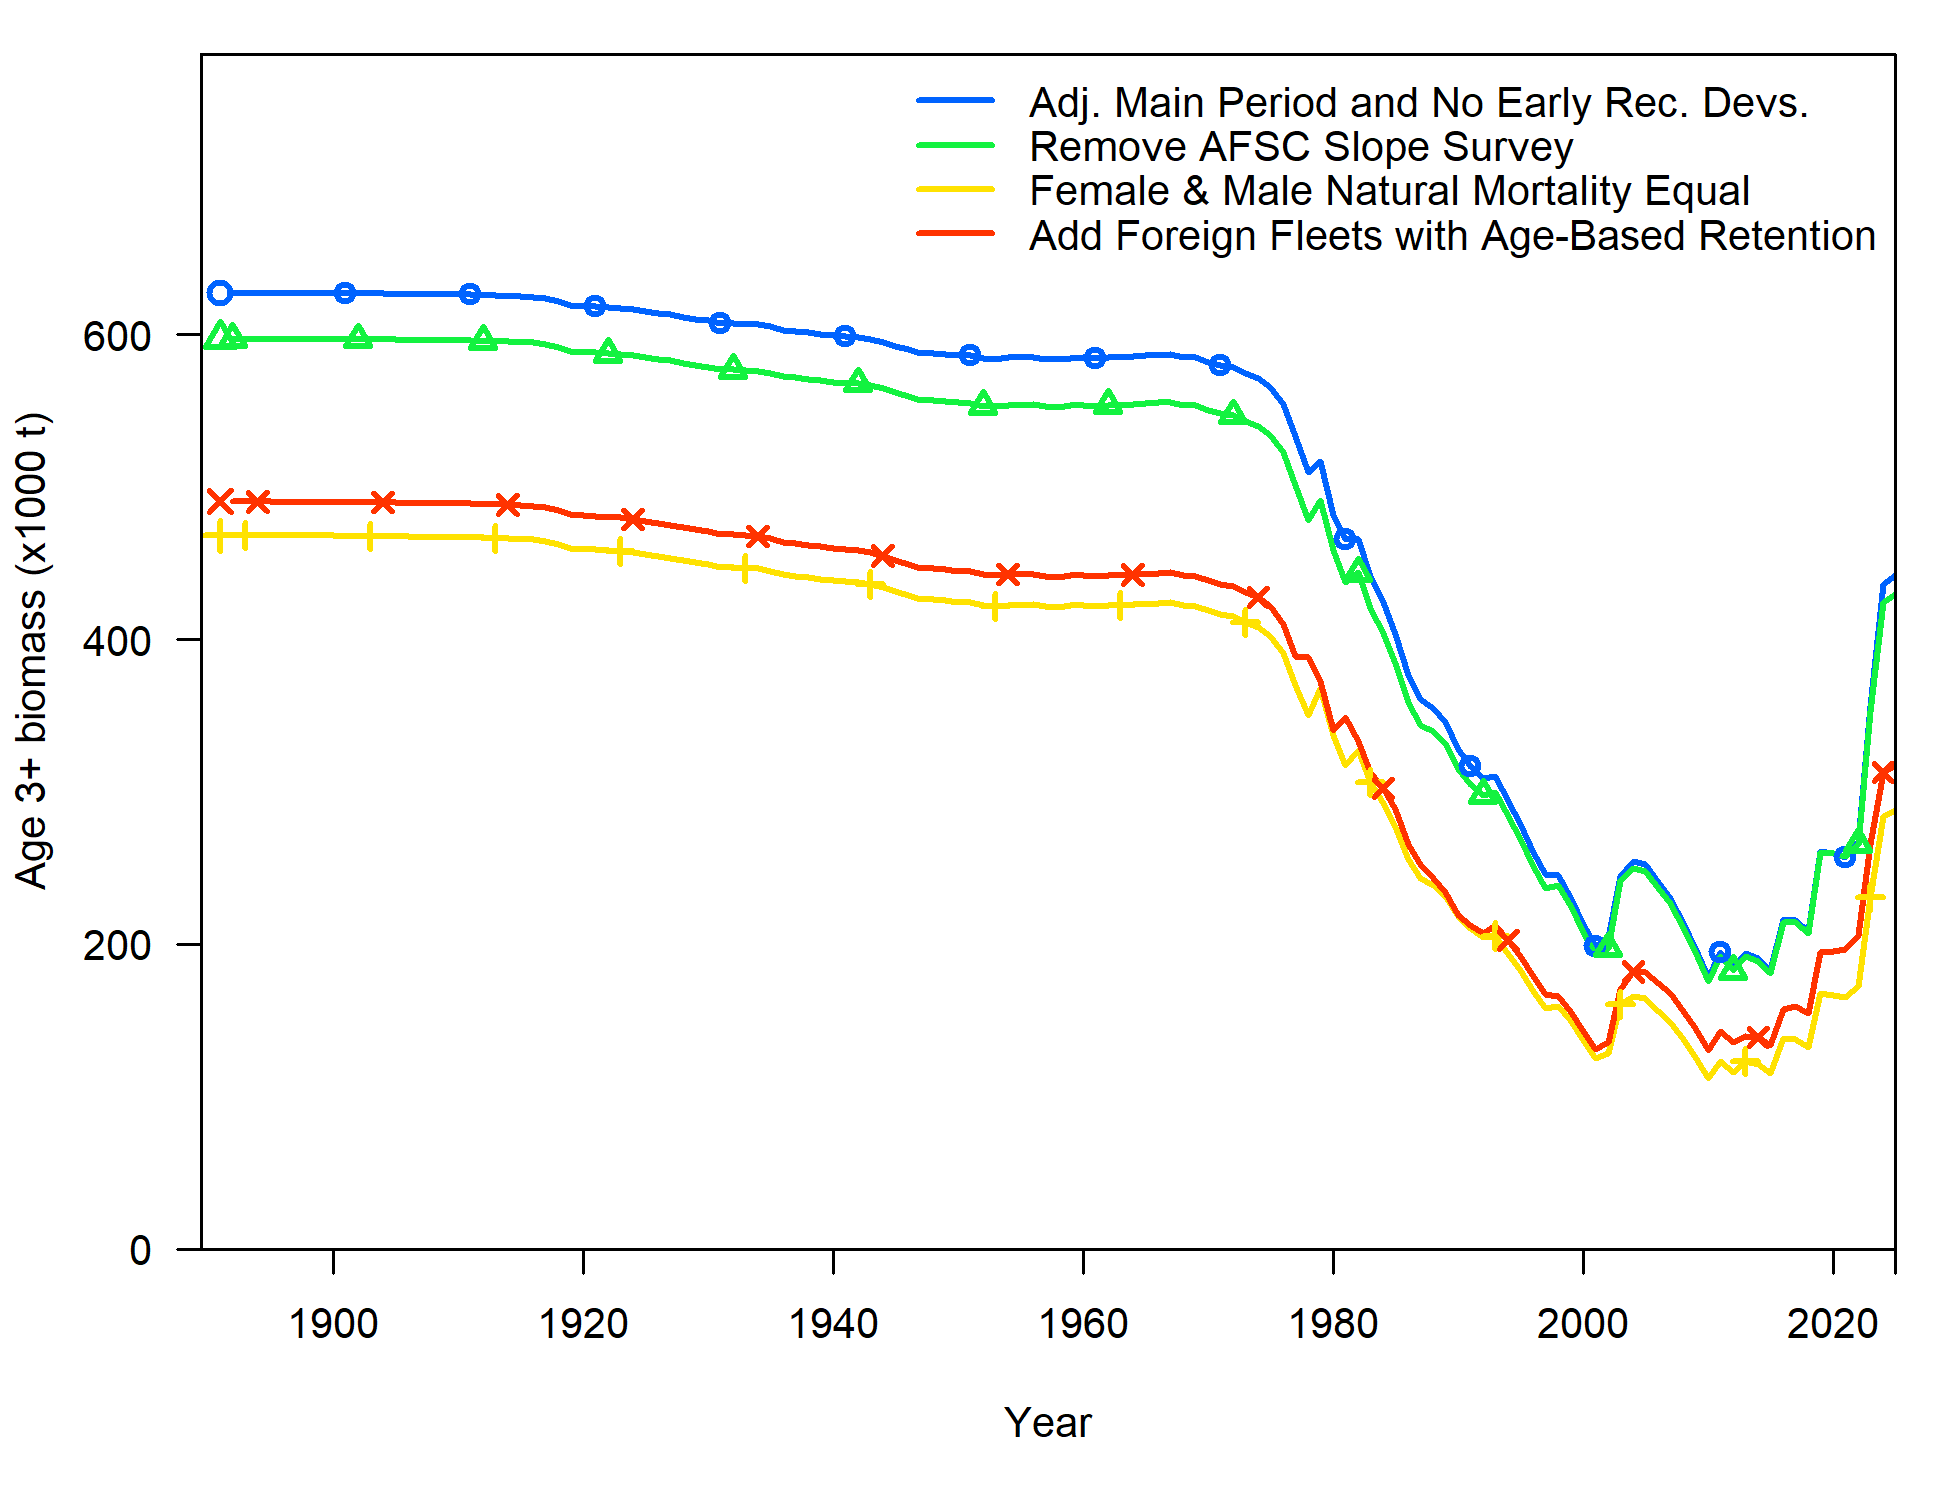
\includegraphics[width=1\linewidth,height=\textheight,keepaspectratio,alt={'Line plot with year on the x-axis and age 3 plus biomass on the y-axis. Model structure bridging where data from AFSC Slope survey were removed from the model, foreign fleets were added to the model estimating retention, and the Triennial survey was split into early and late periods. Each of these changes decreased the estimates of age 3 plus biomass across the time series with age 3 plus biomass estimated at approximately 525,000 metric tons in 1892 and approximately 400,000 metric tons in 2025. Section 3.3.3 model changes from the last assessment describes in detail the changes to estimates.'}]{figures/4_structure_compare18_smrybio.png}

}

\caption{\label{fig-structure-bridge-summary-4}Comparison of estimated
summary biomass for ages 3+ when the model structure is revised.}

\end{figure}%

\begin{figure}[H]

\centering{

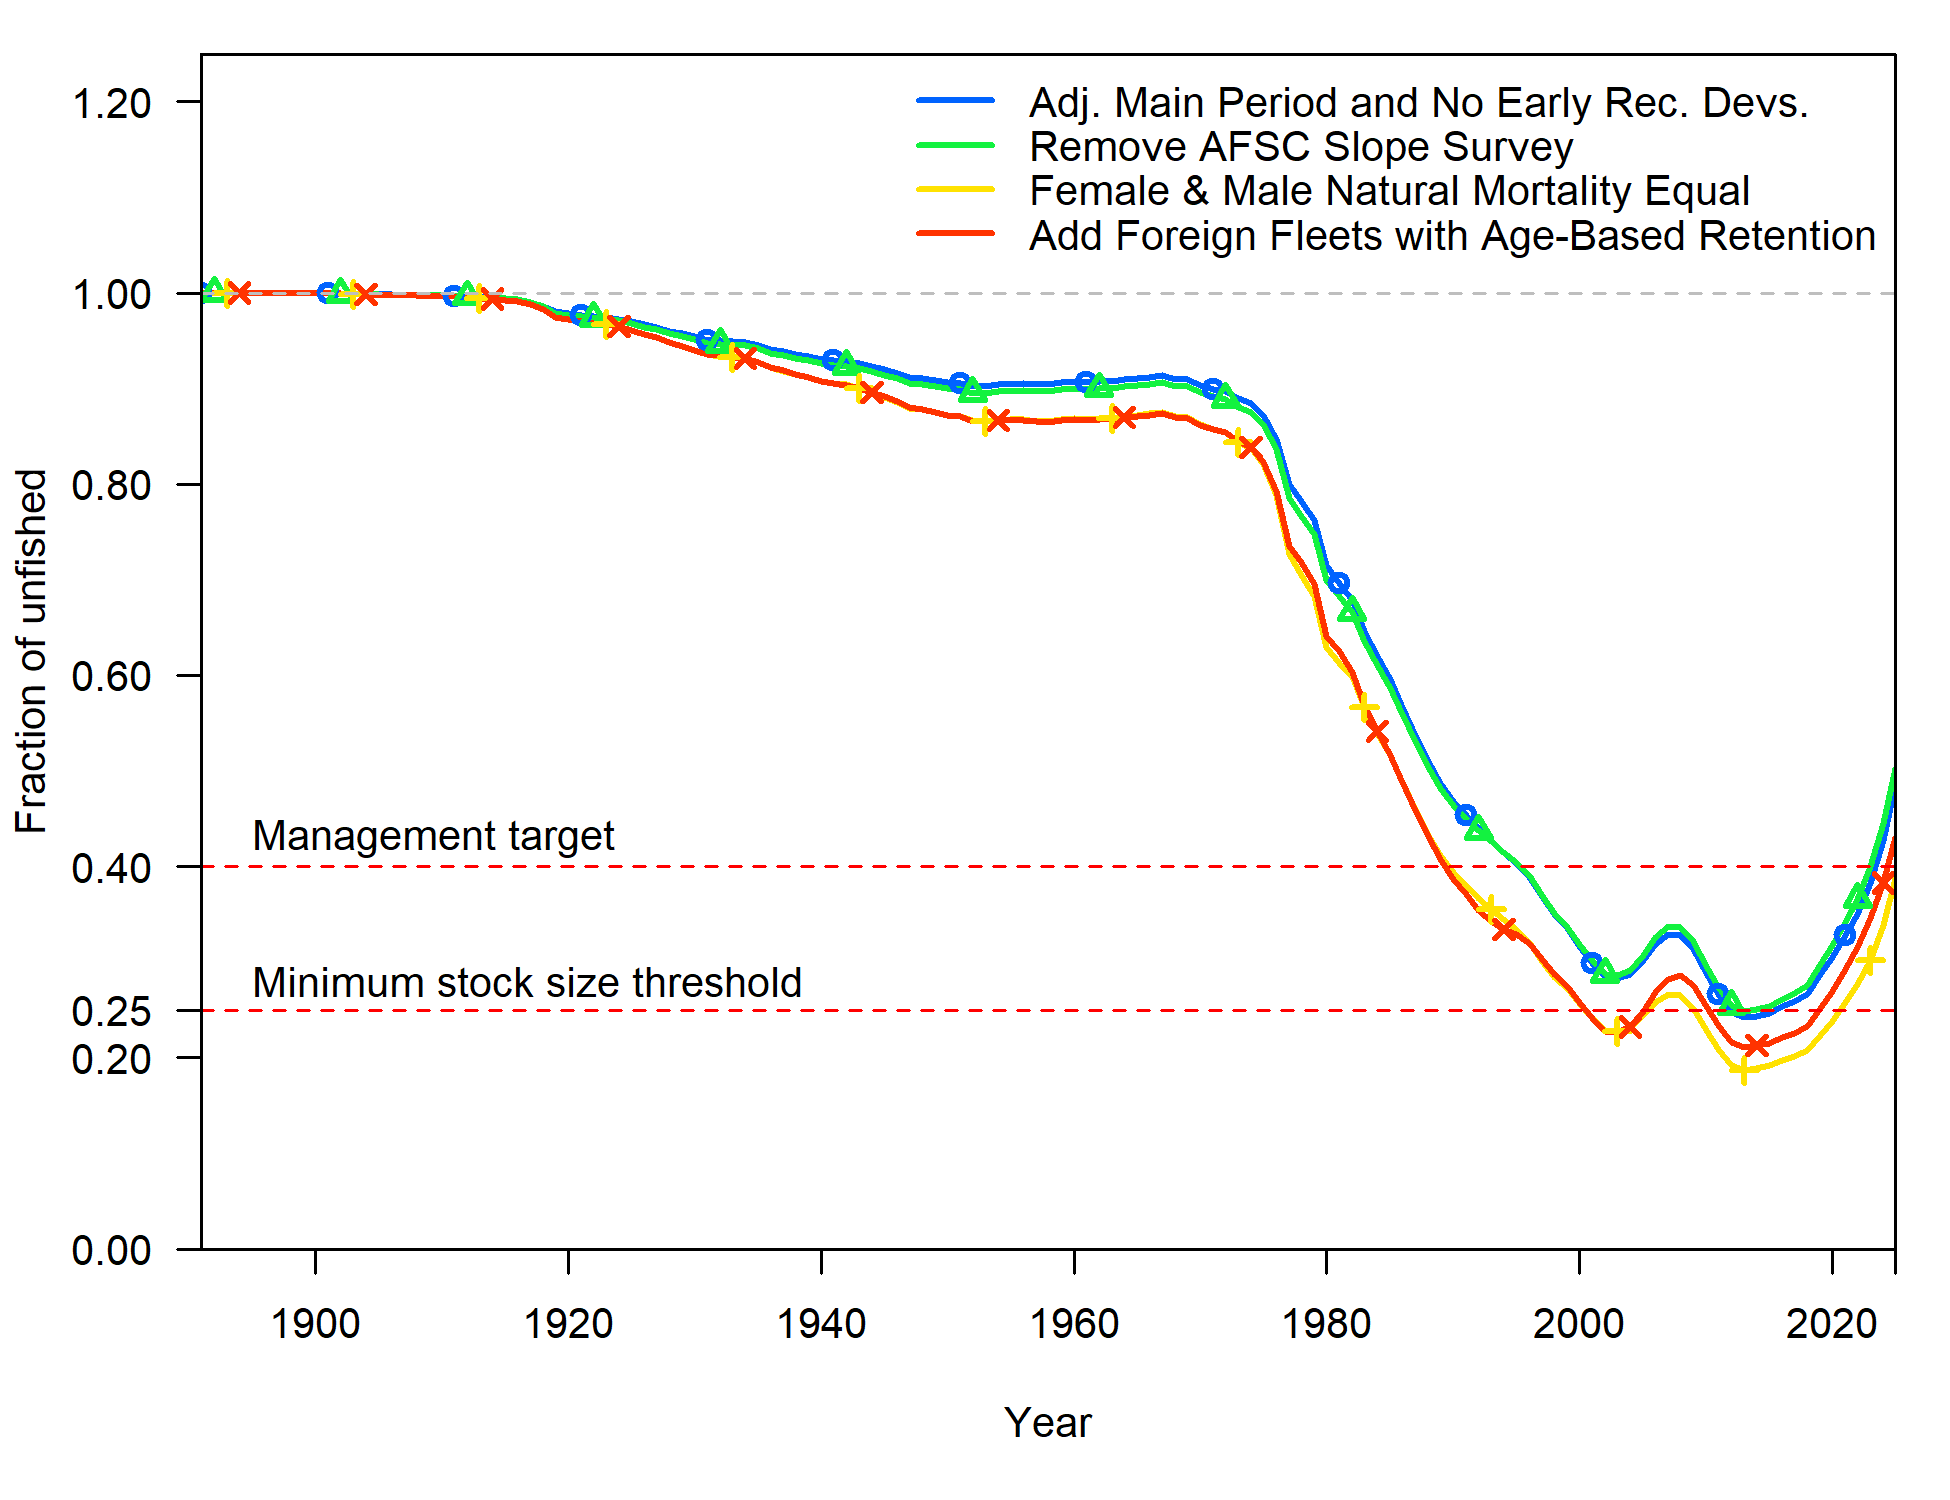
\includegraphics[width=1\linewidth,height=\textheight,keepaspectratio,alt={'Line plot with year on the x-axis and fraction of unfished on the y-axis. Model structure bridging where data from AFSC Slope survey were removed from the model, foreign fleets were added to the model estimating retention, and the Triennial survey was split into early and late periods. Each of these changes resulted in similar estiamtes of fraction of unfished across the time series with the fraction of unfished estimated at approximately 55 percent in 2025. Section 3.3.3 model changes from the last assessment describes in detail the changes to estimates.'}]{figures/4_structure_compare3_Bratio.png}

}

\caption{\label{fig-structure-bridge-depl-4}Comparison of estimated
fraction unfished (i.e., stock status) when the model structure is
revised.}

\end{figure}%

\begin{figure}[H]

\centering{

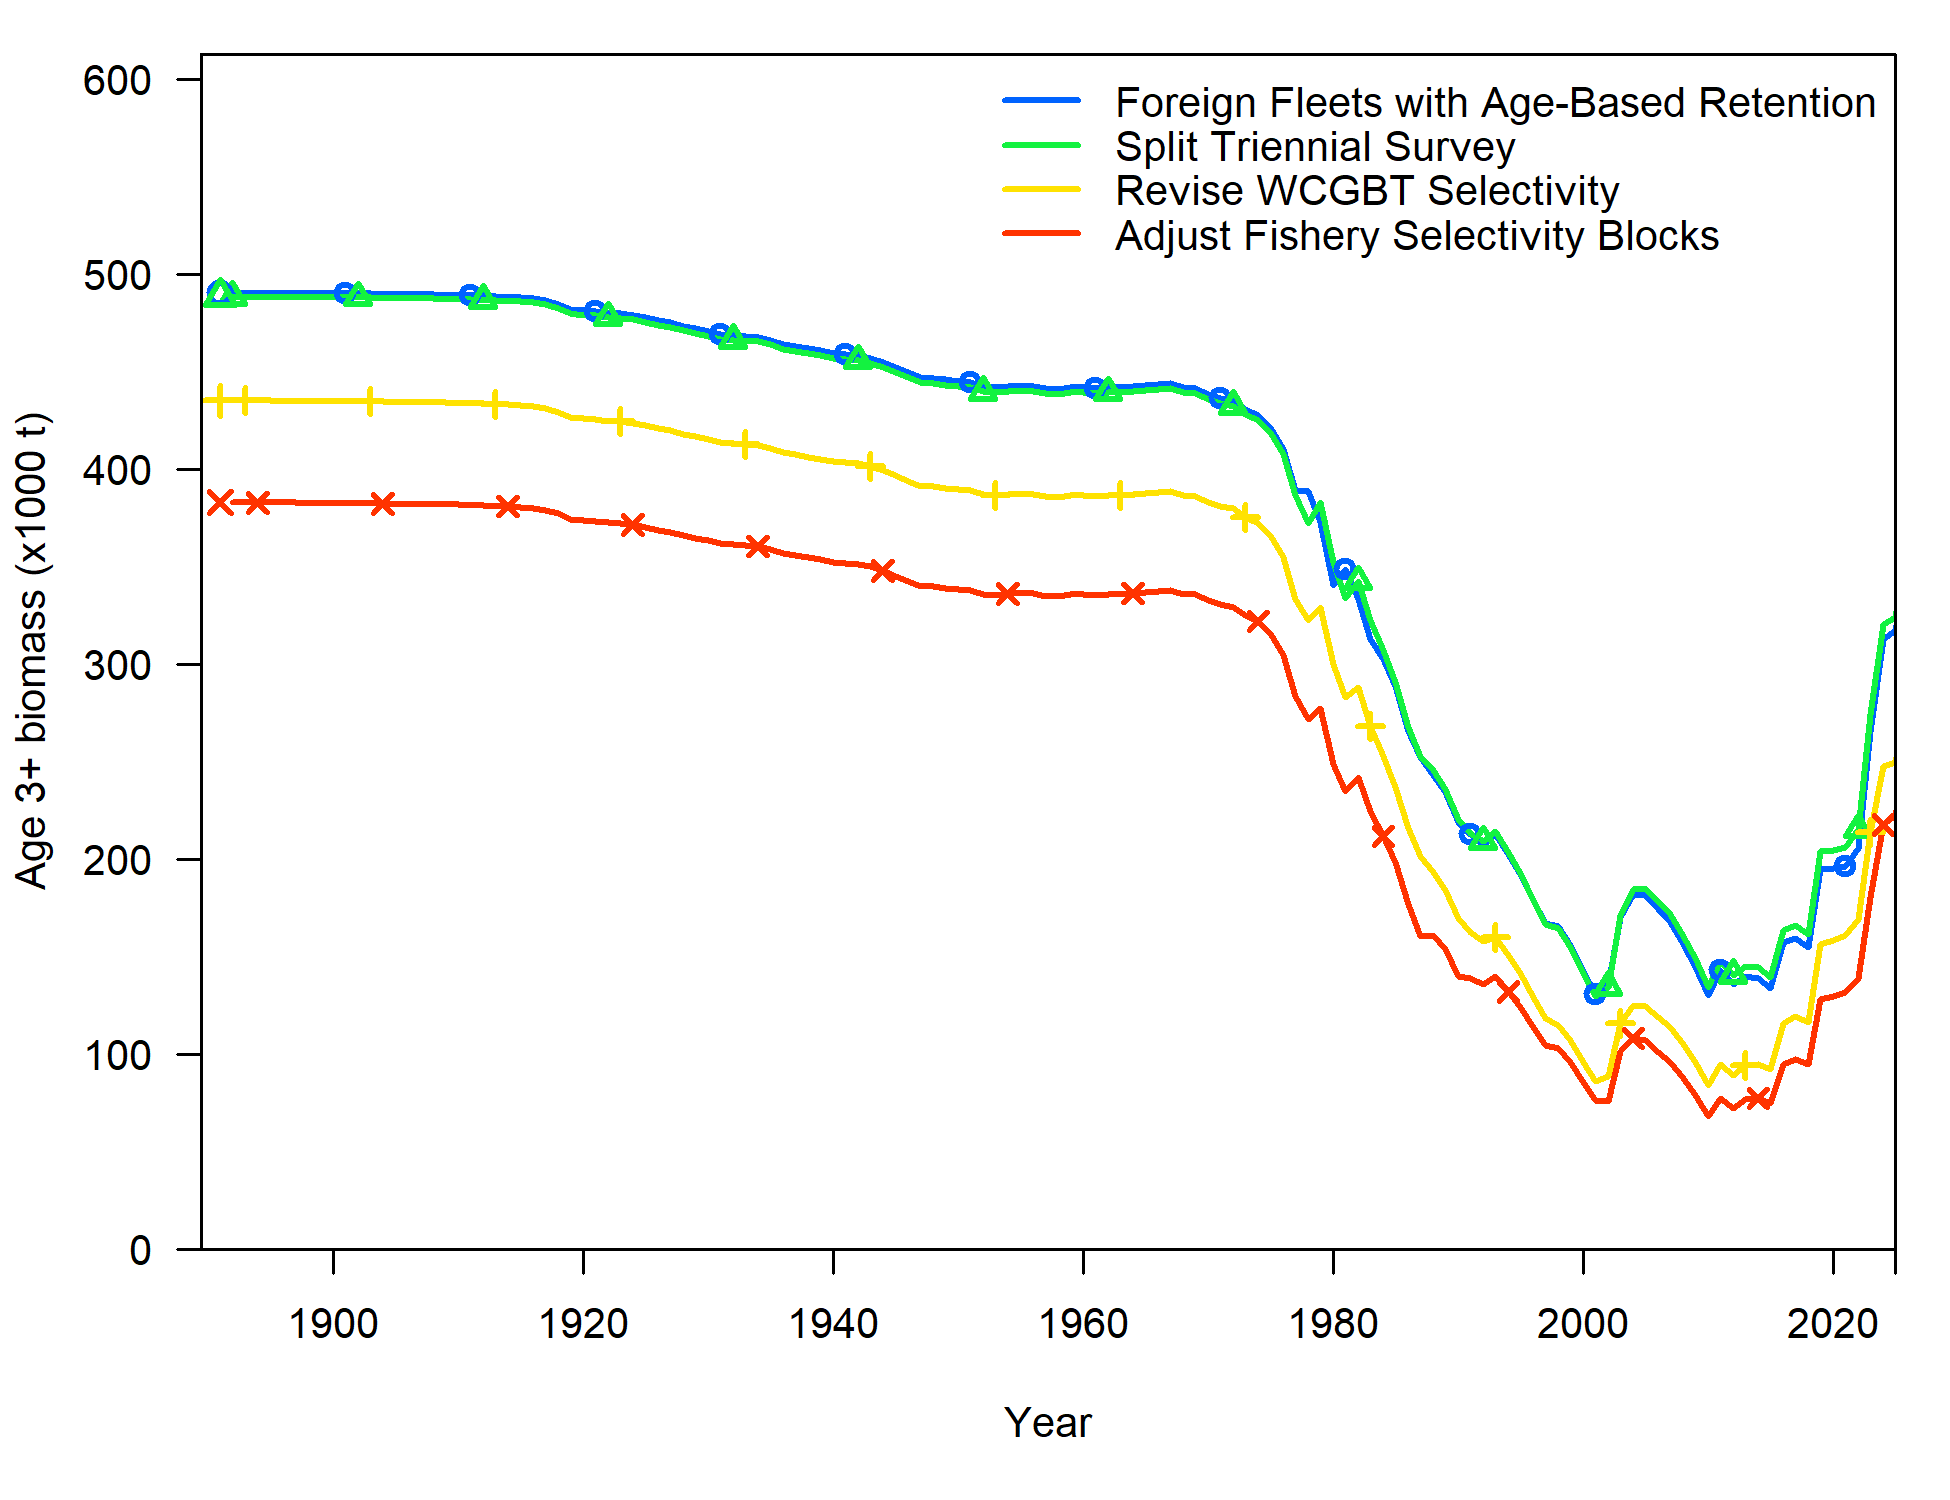
\includegraphics[width=1\linewidth,height=\textheight,keepaspectratio,alt={'Line plot with year on the x-axis and age 3 plus biomass on the y-axis. Model structure bridging where the selectivity of the WCGBTS was updated and discard fleets were used to account for total mortality rather than estimating retention. The model with discard fleet decreased the estimates of age 3 plus biomass across the time series with age 3 plus biomass estimated at approximately 425,000 metric tons in 1892 and approximately 275,000 metric tons in 2025. Section 3.3.3 model changes from the last assessment describes in detail the changes to estimates.'}]{figures/5_structure_compare18_smrybio.png}

}

\caption{\label{fig-structure-bridge-summary-5}Comparison of estimated
summary biomass for ages 3+ when the model structure is revised.}

\end{figure}%

\begin{figure}[H]

\centering{

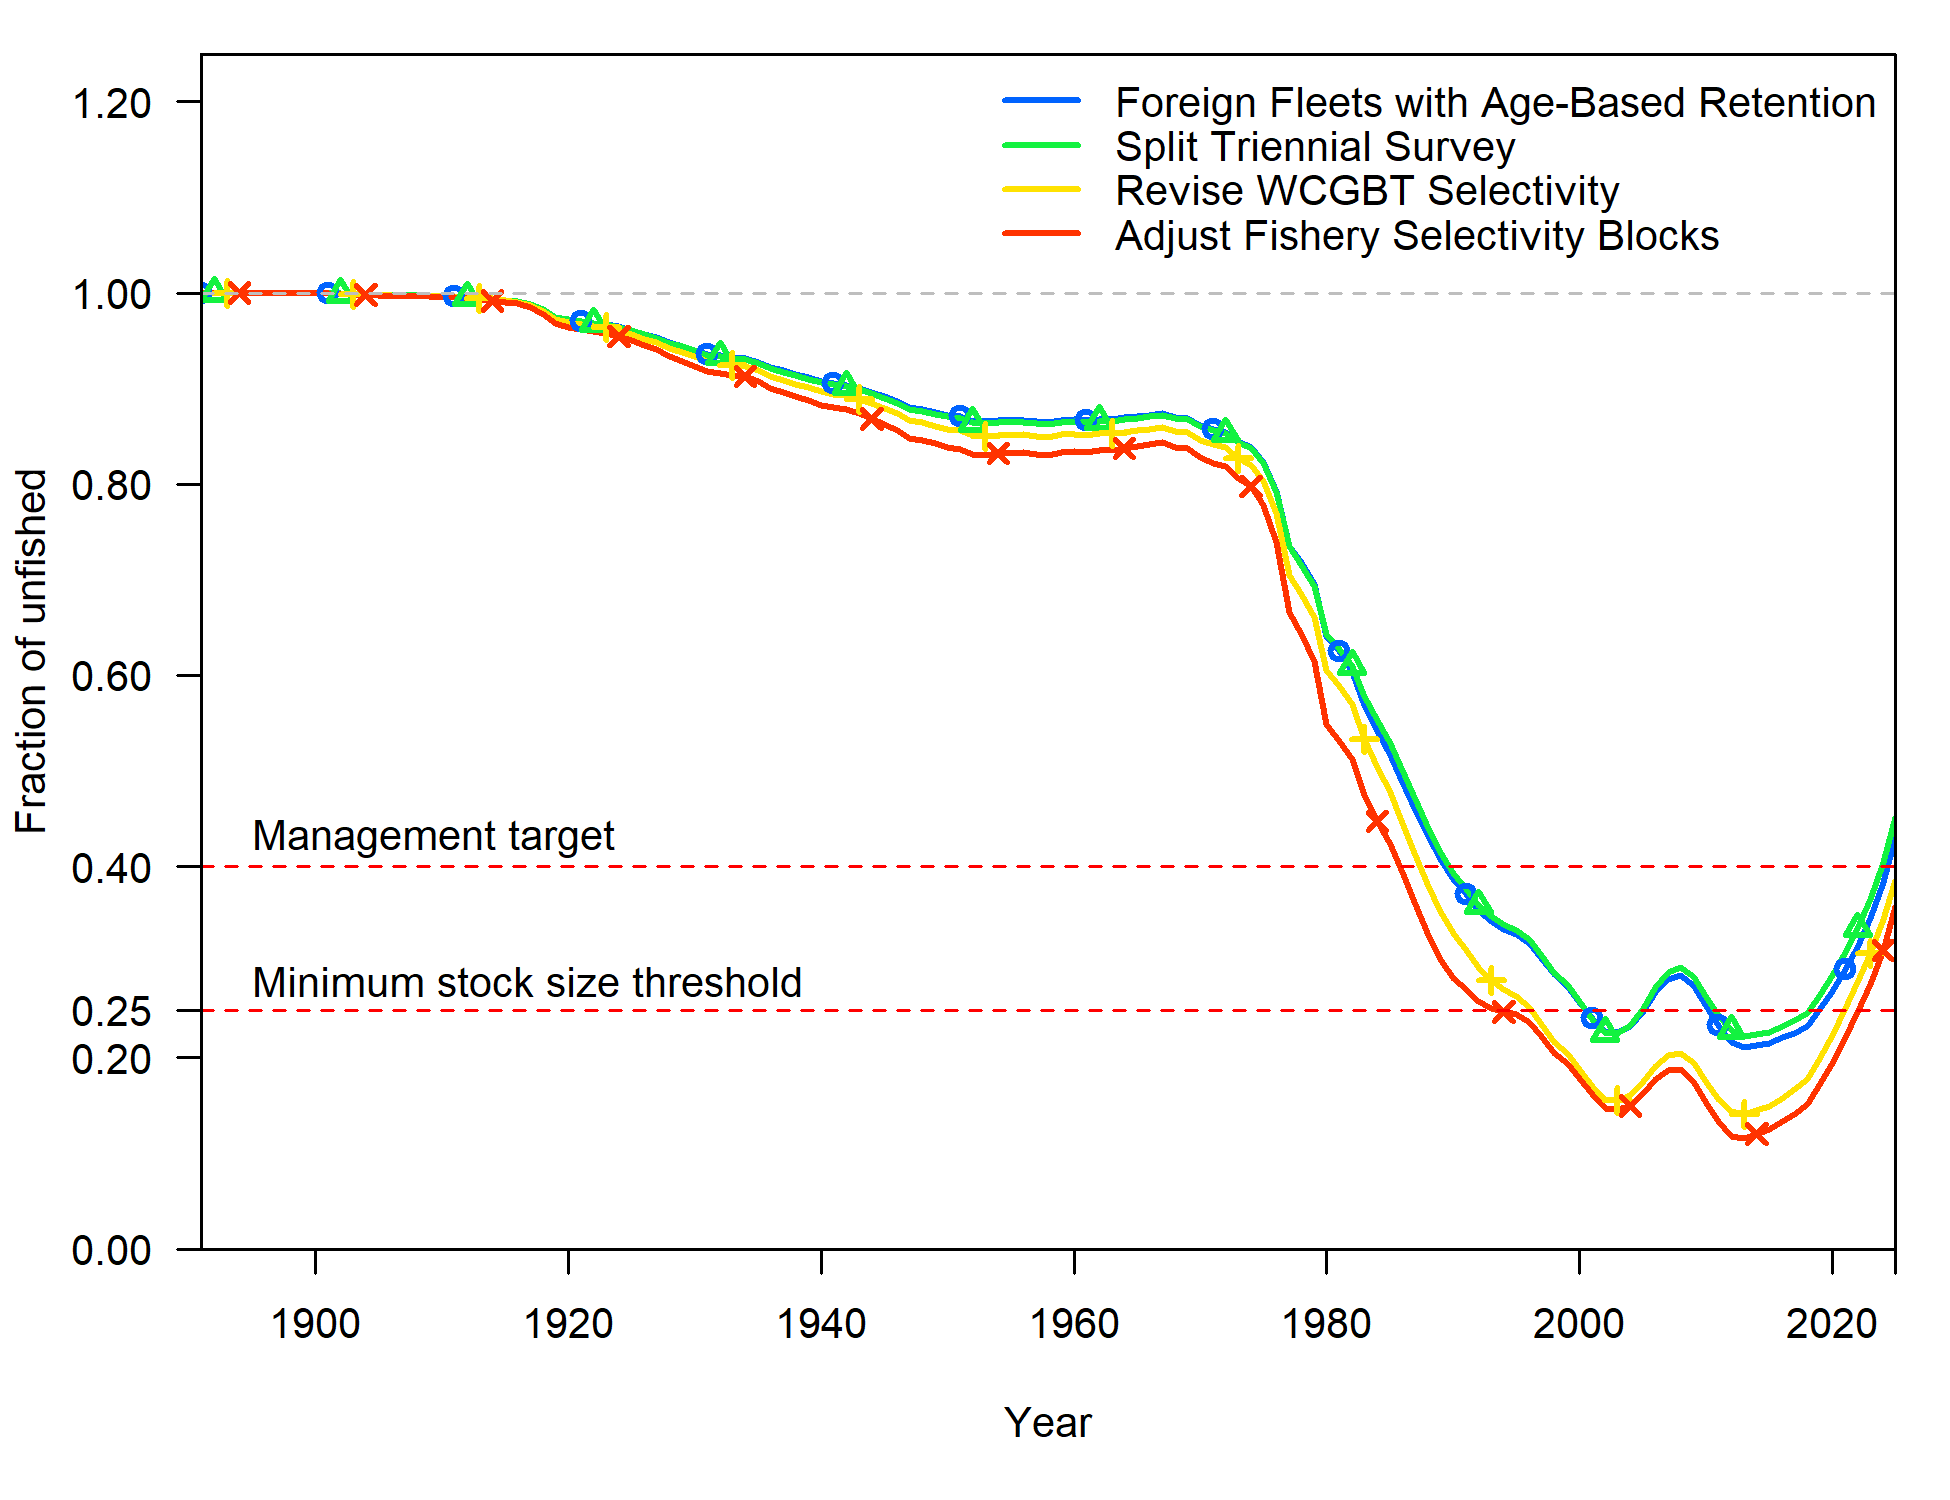
\includegraphics[width=1\linewidth,height=\textheight,keepaspectratio,alt={'Line plot with year on the x-axis and fraction of unfished on the y-axis. Model structure bridging where the selectivity of the WCGBTS was updated and discard fleets were used to account for total mortality rather than estimating retention. Each of these changes resulted in a more depleted population being estimated from 1970 through 2025 with the fraction of unfished in 2025 estimated at approximately 30 percent. Section 3.3.3 model changes from the last assessment describes in detail the changes to estimates.'}]{figures/5_structure_compare3_Bratio.png}

}

\caption{\label{fig-structure-bridge-depl-5}Comparison of estimated
fraction unfished (i.e., stock status) when the model structure is
revised.}

\end{figure}%

\begin{figure}[H]

\centering{

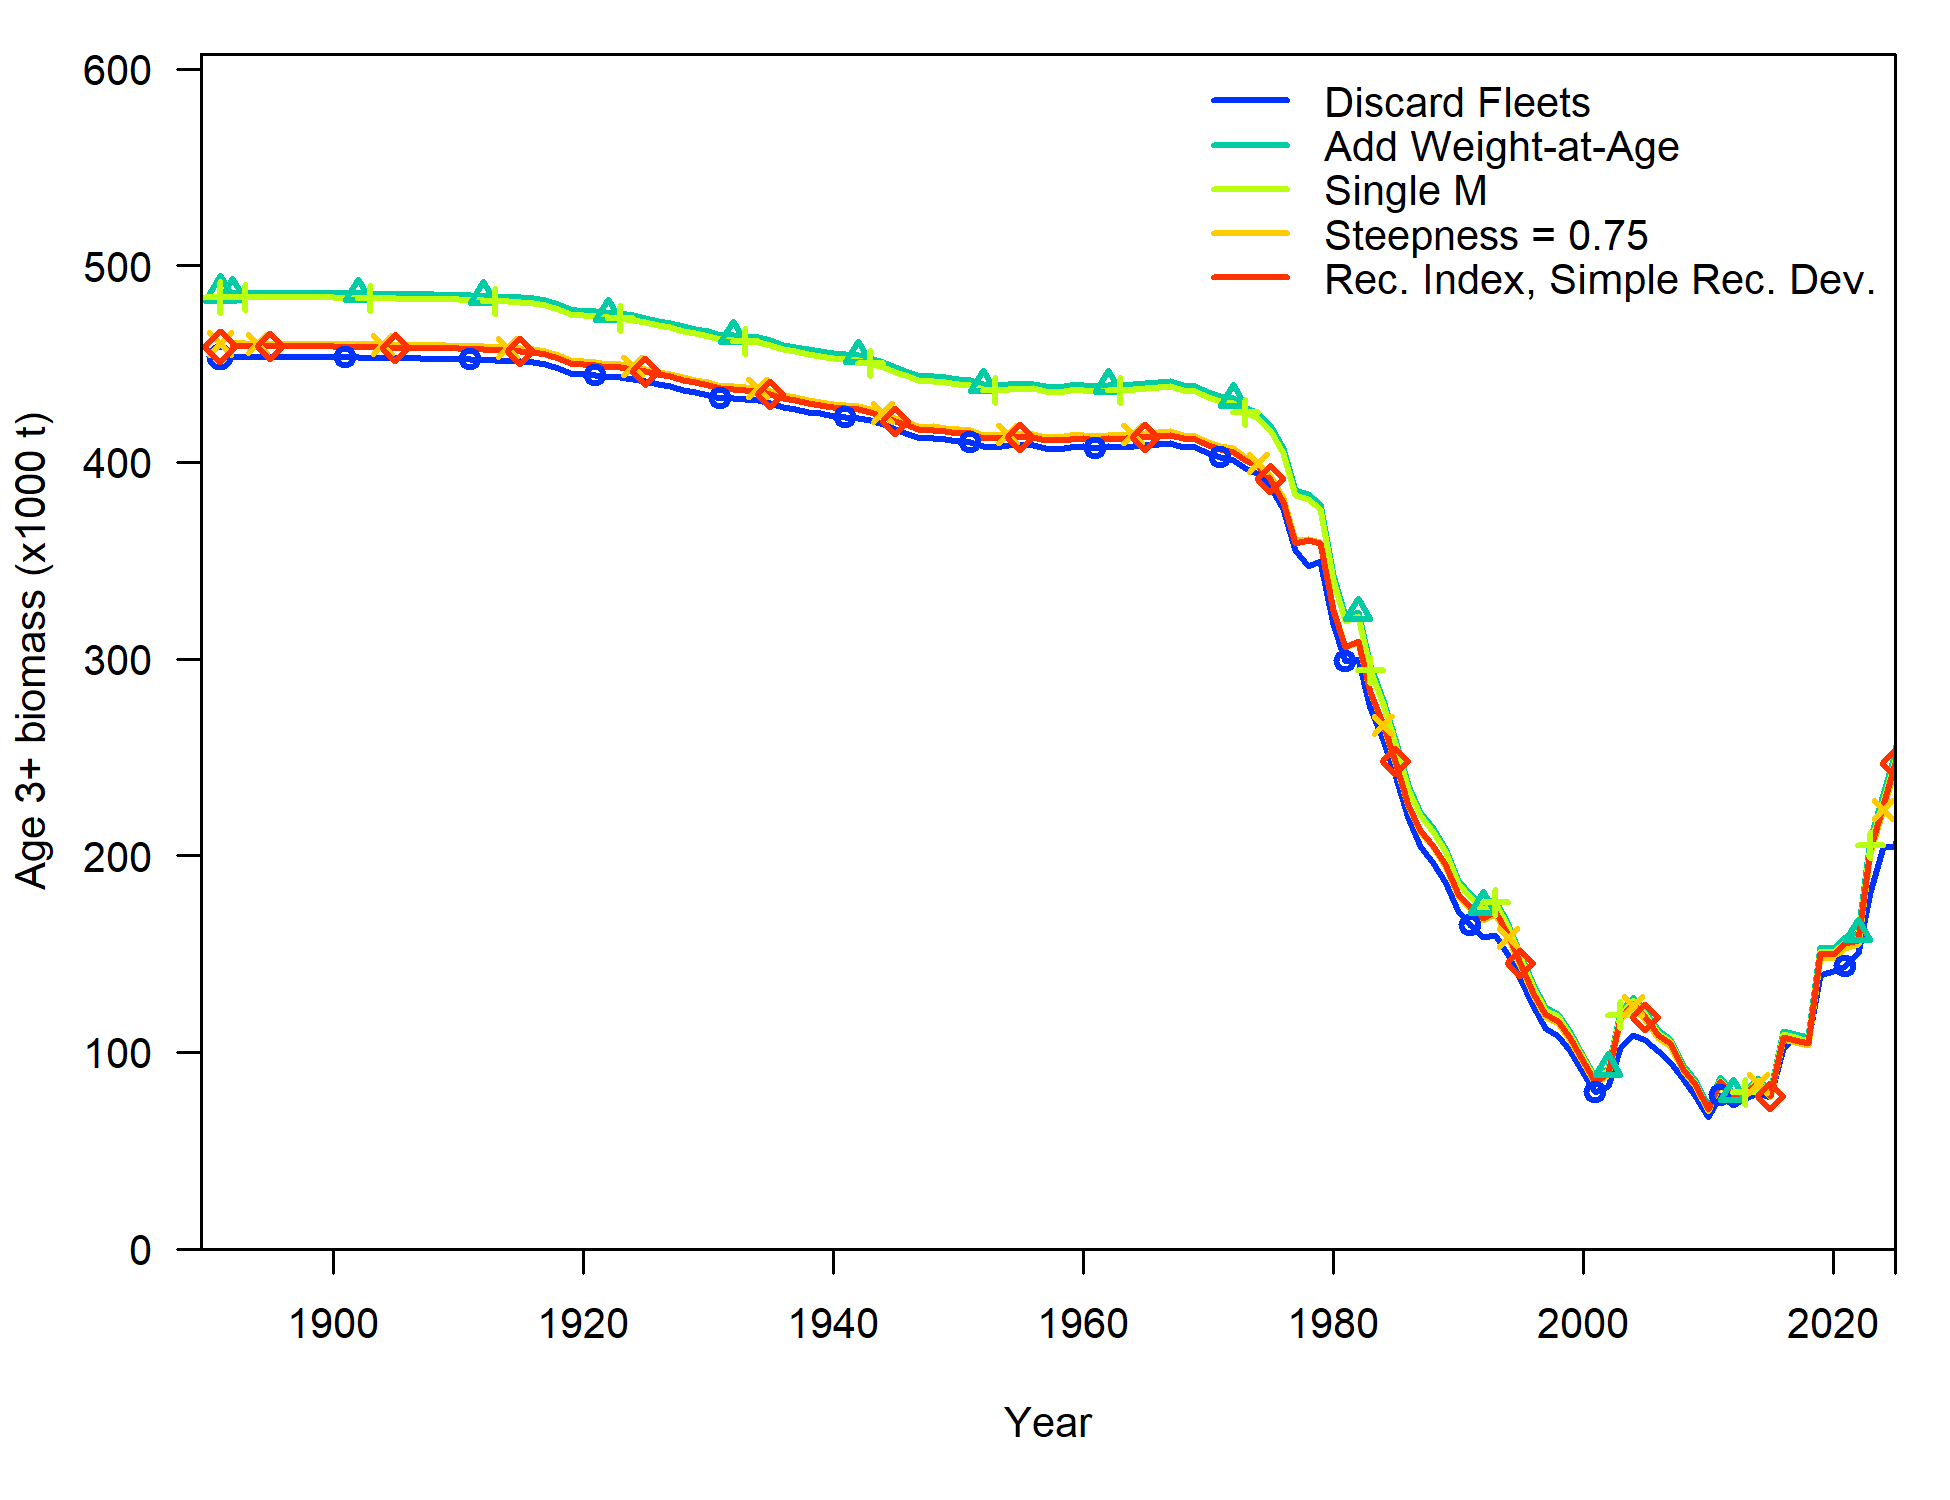
\includegraphics[width=1\linewidth,height=\textheight,keepaspectratio,alt={'Line plot with year on the x-axis and age 3 plus biomass on the y-axis. Final model structure bridging where empirical weight-at-age is added, natural mortality for males and females is assumed equal, steepness is set at 0.75, and annual recruitment deviations are estimated as simple vector. The estimates of age 3 plus biomass is similar across all bridging models. Section 3.3.3 model changes from the last assessment describes in detail the changes to estimates.'}]{figures/6_structure_compare18_smrybio.png}

}

\caption{\label{fig-structure-bridge-summary-6}Comparison of estimated
summary biomass for ages 3+ when the model structure is revised.}

\end{figure}%

\begin{figure}[H]

\centering{

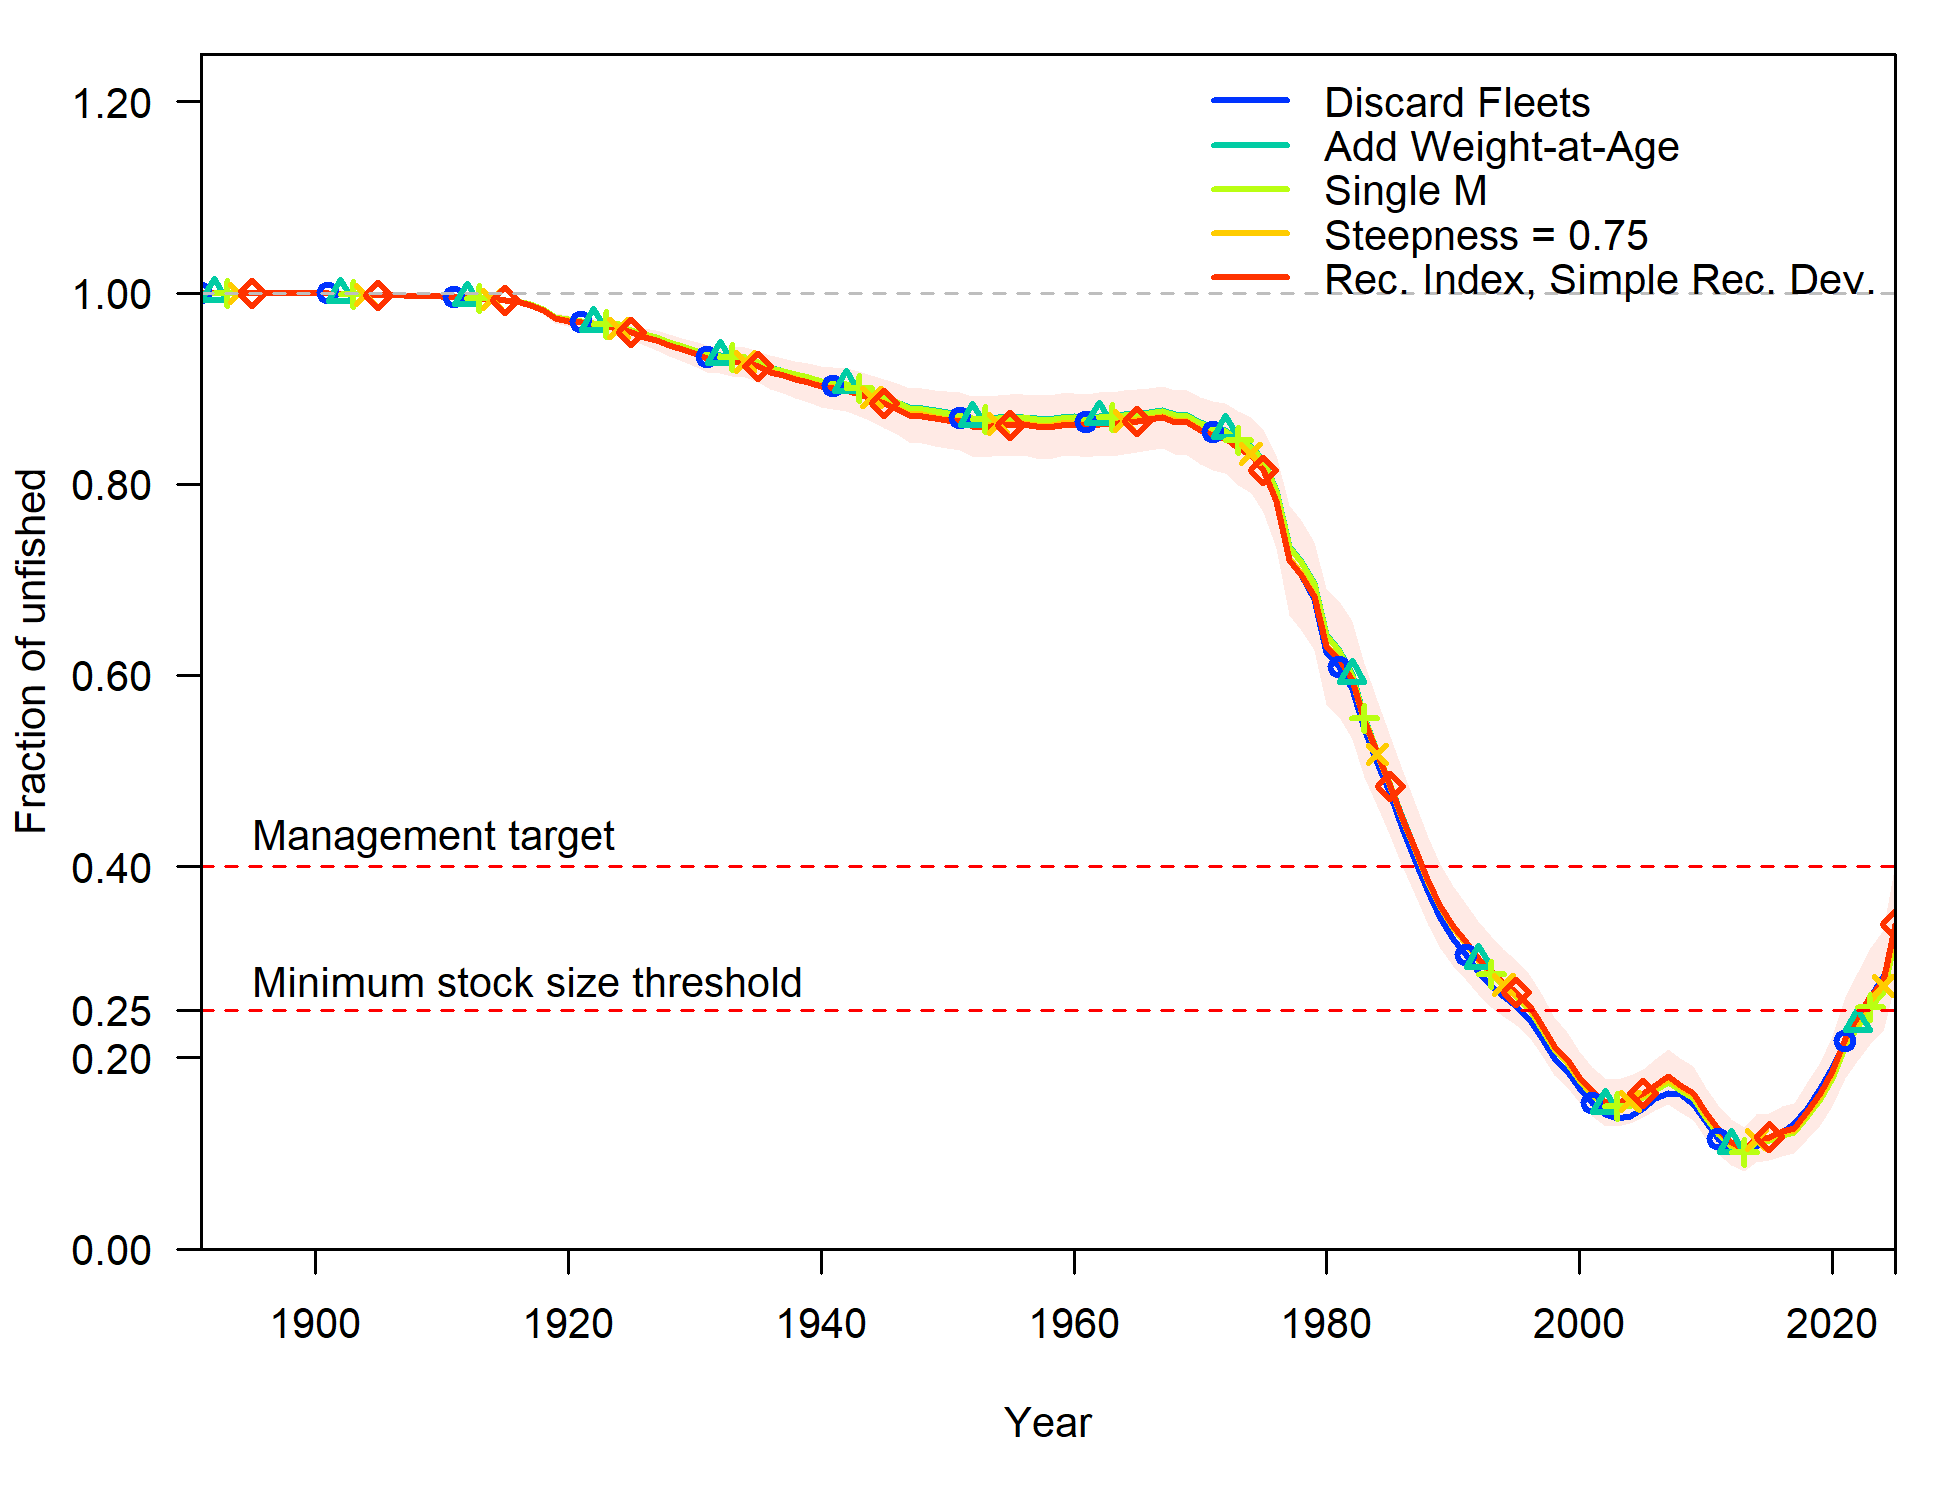
\includegraphics[width=1\linewidth,height=\textheight,keepaspectratio,alt={'Line plot with year on the x-axis and fraction of unfished on the y-axis. Final model structure bridging where empirical weight-at-age is added, natural mortality for males and females is assumed equal, steepness is set at 0.75, and annual recruitment deviations are estimated as simple vector. The estimates of fraction of unfished is similar across all bridging models. Section 3.3.3 model changes from the last assessment describes in detail the changes to estimates.'}]{figures/6_structure_compare4_Bratio_uncertainty.png}

}

\caption{\label{fig-structure-bridge-depl-6}Comparison of estimated
fraction unfished (e.g., stock status) when the model structure is
revised.}

\end{figure}%

\subsection{Paramters}\label{paramters}

\begin{figure}[H]

\centering{

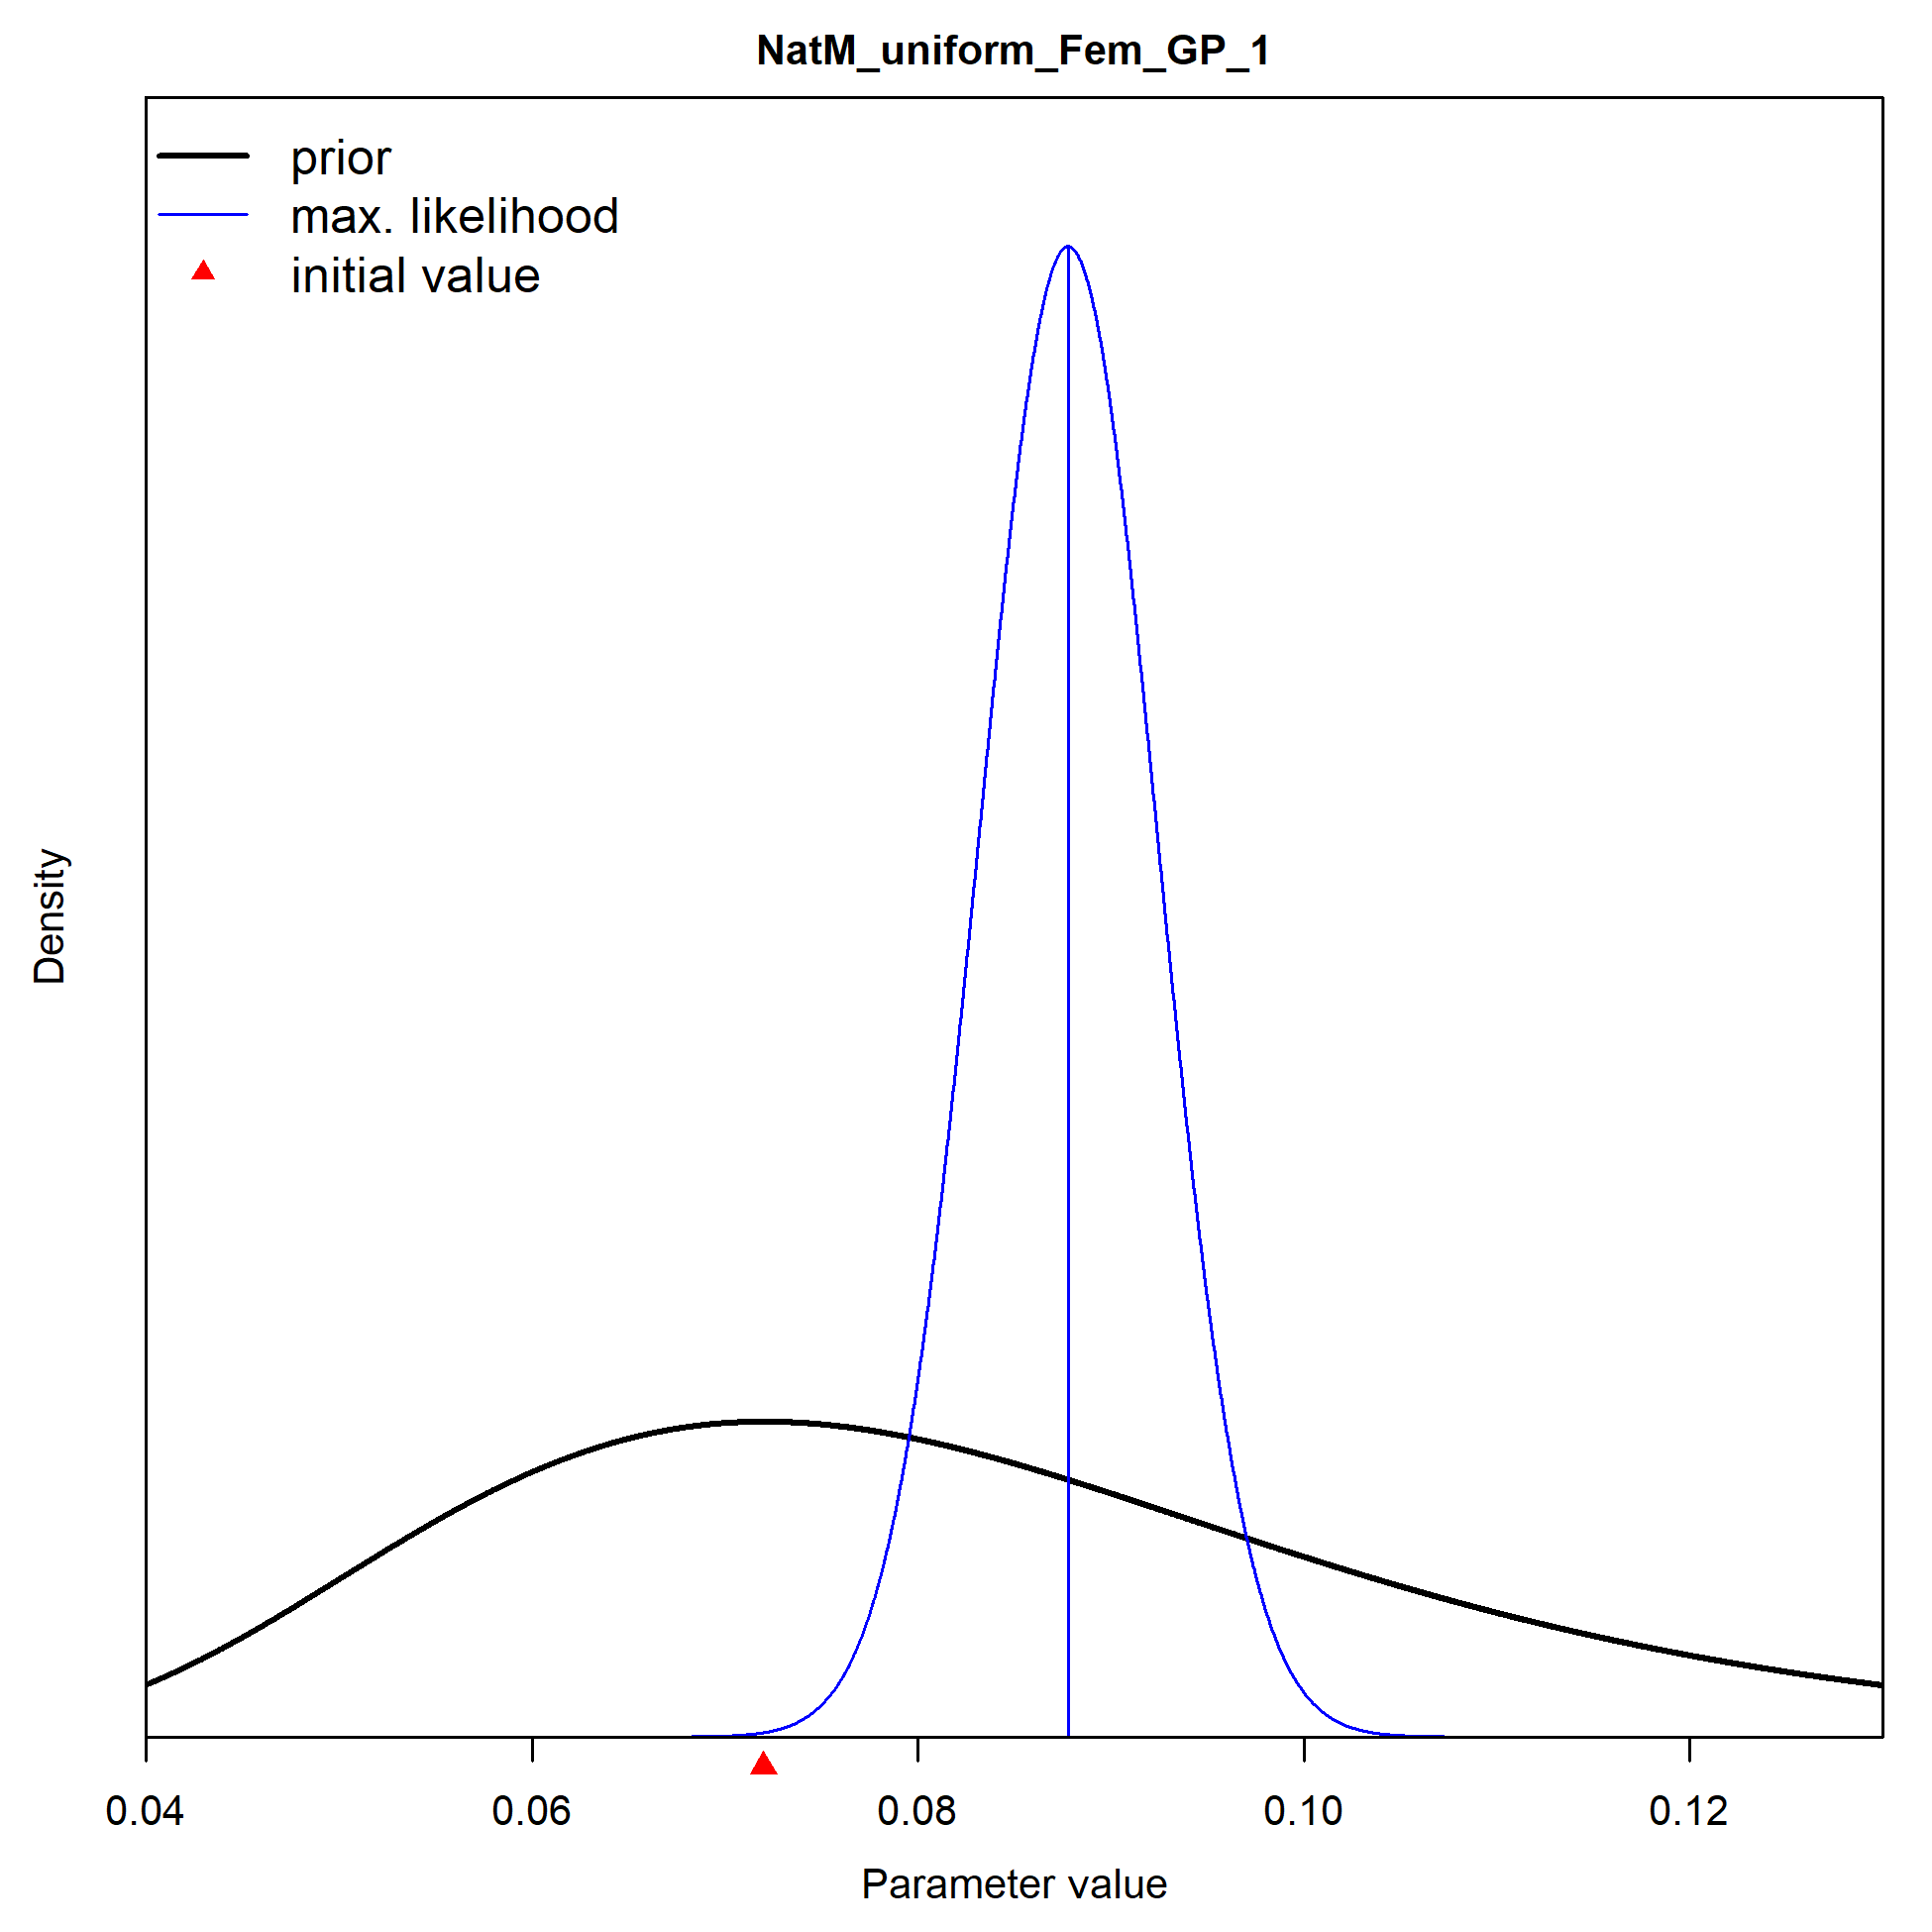
\includegraphics[width=1\linewidth,height=\textheight,keepaspectratio,alt={'Density plot with natural mortality on the x-axis and density on the y-axis. The natural mortality prior has a wide distribution ranging from less than 0.04 to greater than 0.13 with peak density at the prior of 0.075.  The model estimated value is 0.088 with uncertainty ranging from 0.075 to 0.102.'}]{figures/parameter_distributions_pageNaN.png}

}

\caption{\label{fig-m-est-prior}Prior distributions and parameter
estimates for natural mortality. Black lines show prior distributions,
blue lines show maximum likelihood estimate and associated uncertainty.}

\end{figure}%

\pagebreak

\begin{figure}[H]

\centering{

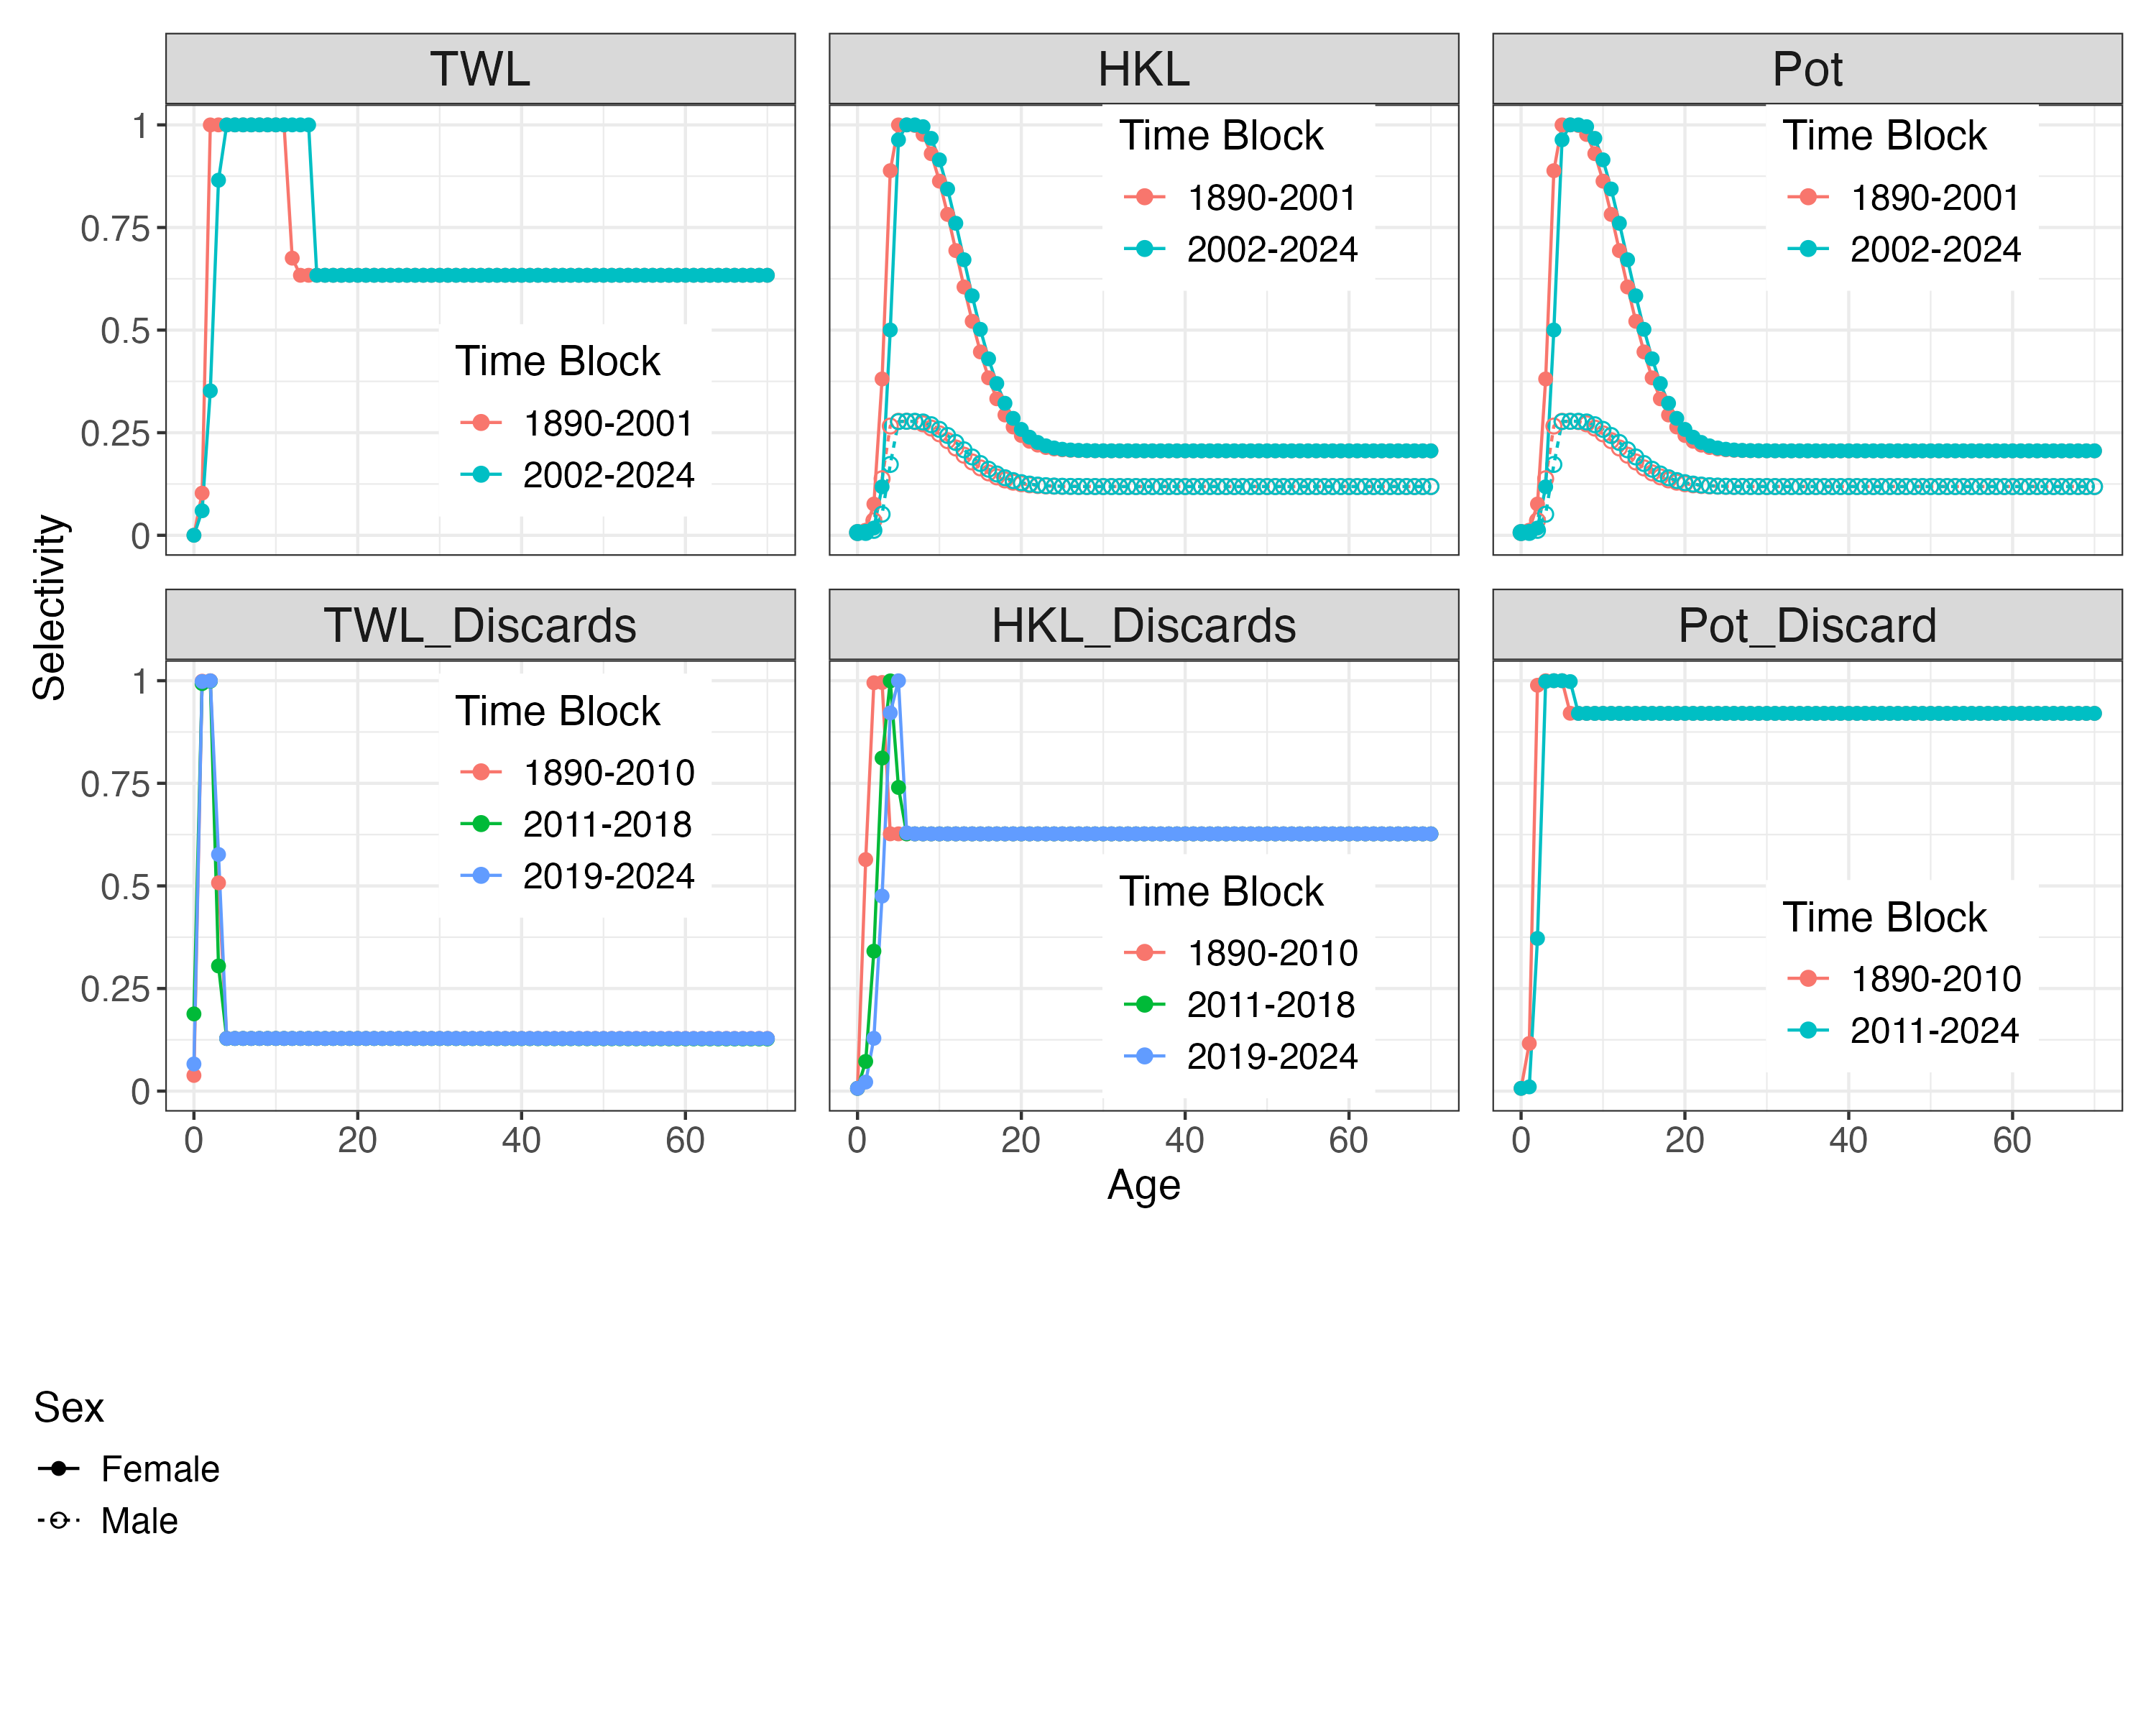
\includegraphics[width=1\linewidth,height=\textheight,keepaspectratio,alt={'Line plot with age in years on the x-axis and selectivity ranging from 0 to 1 on the y-axis with a panel for each fishery fleet in the model.  Selectivity for each fishery fleet is dome shaped with reduced selectivity for older ages.  Selectivity for hook-and-line and pot gears were assumed equal with higher selectivity for females compared to males.'}]{figures/fishery_selex_timeblocks.png}

}

\caption{\label{fig-fishery-selex}Selectivity curves for each fishery
fleet in the base model.}

\end{figure}%

\begin{figure}[H]

\centering{

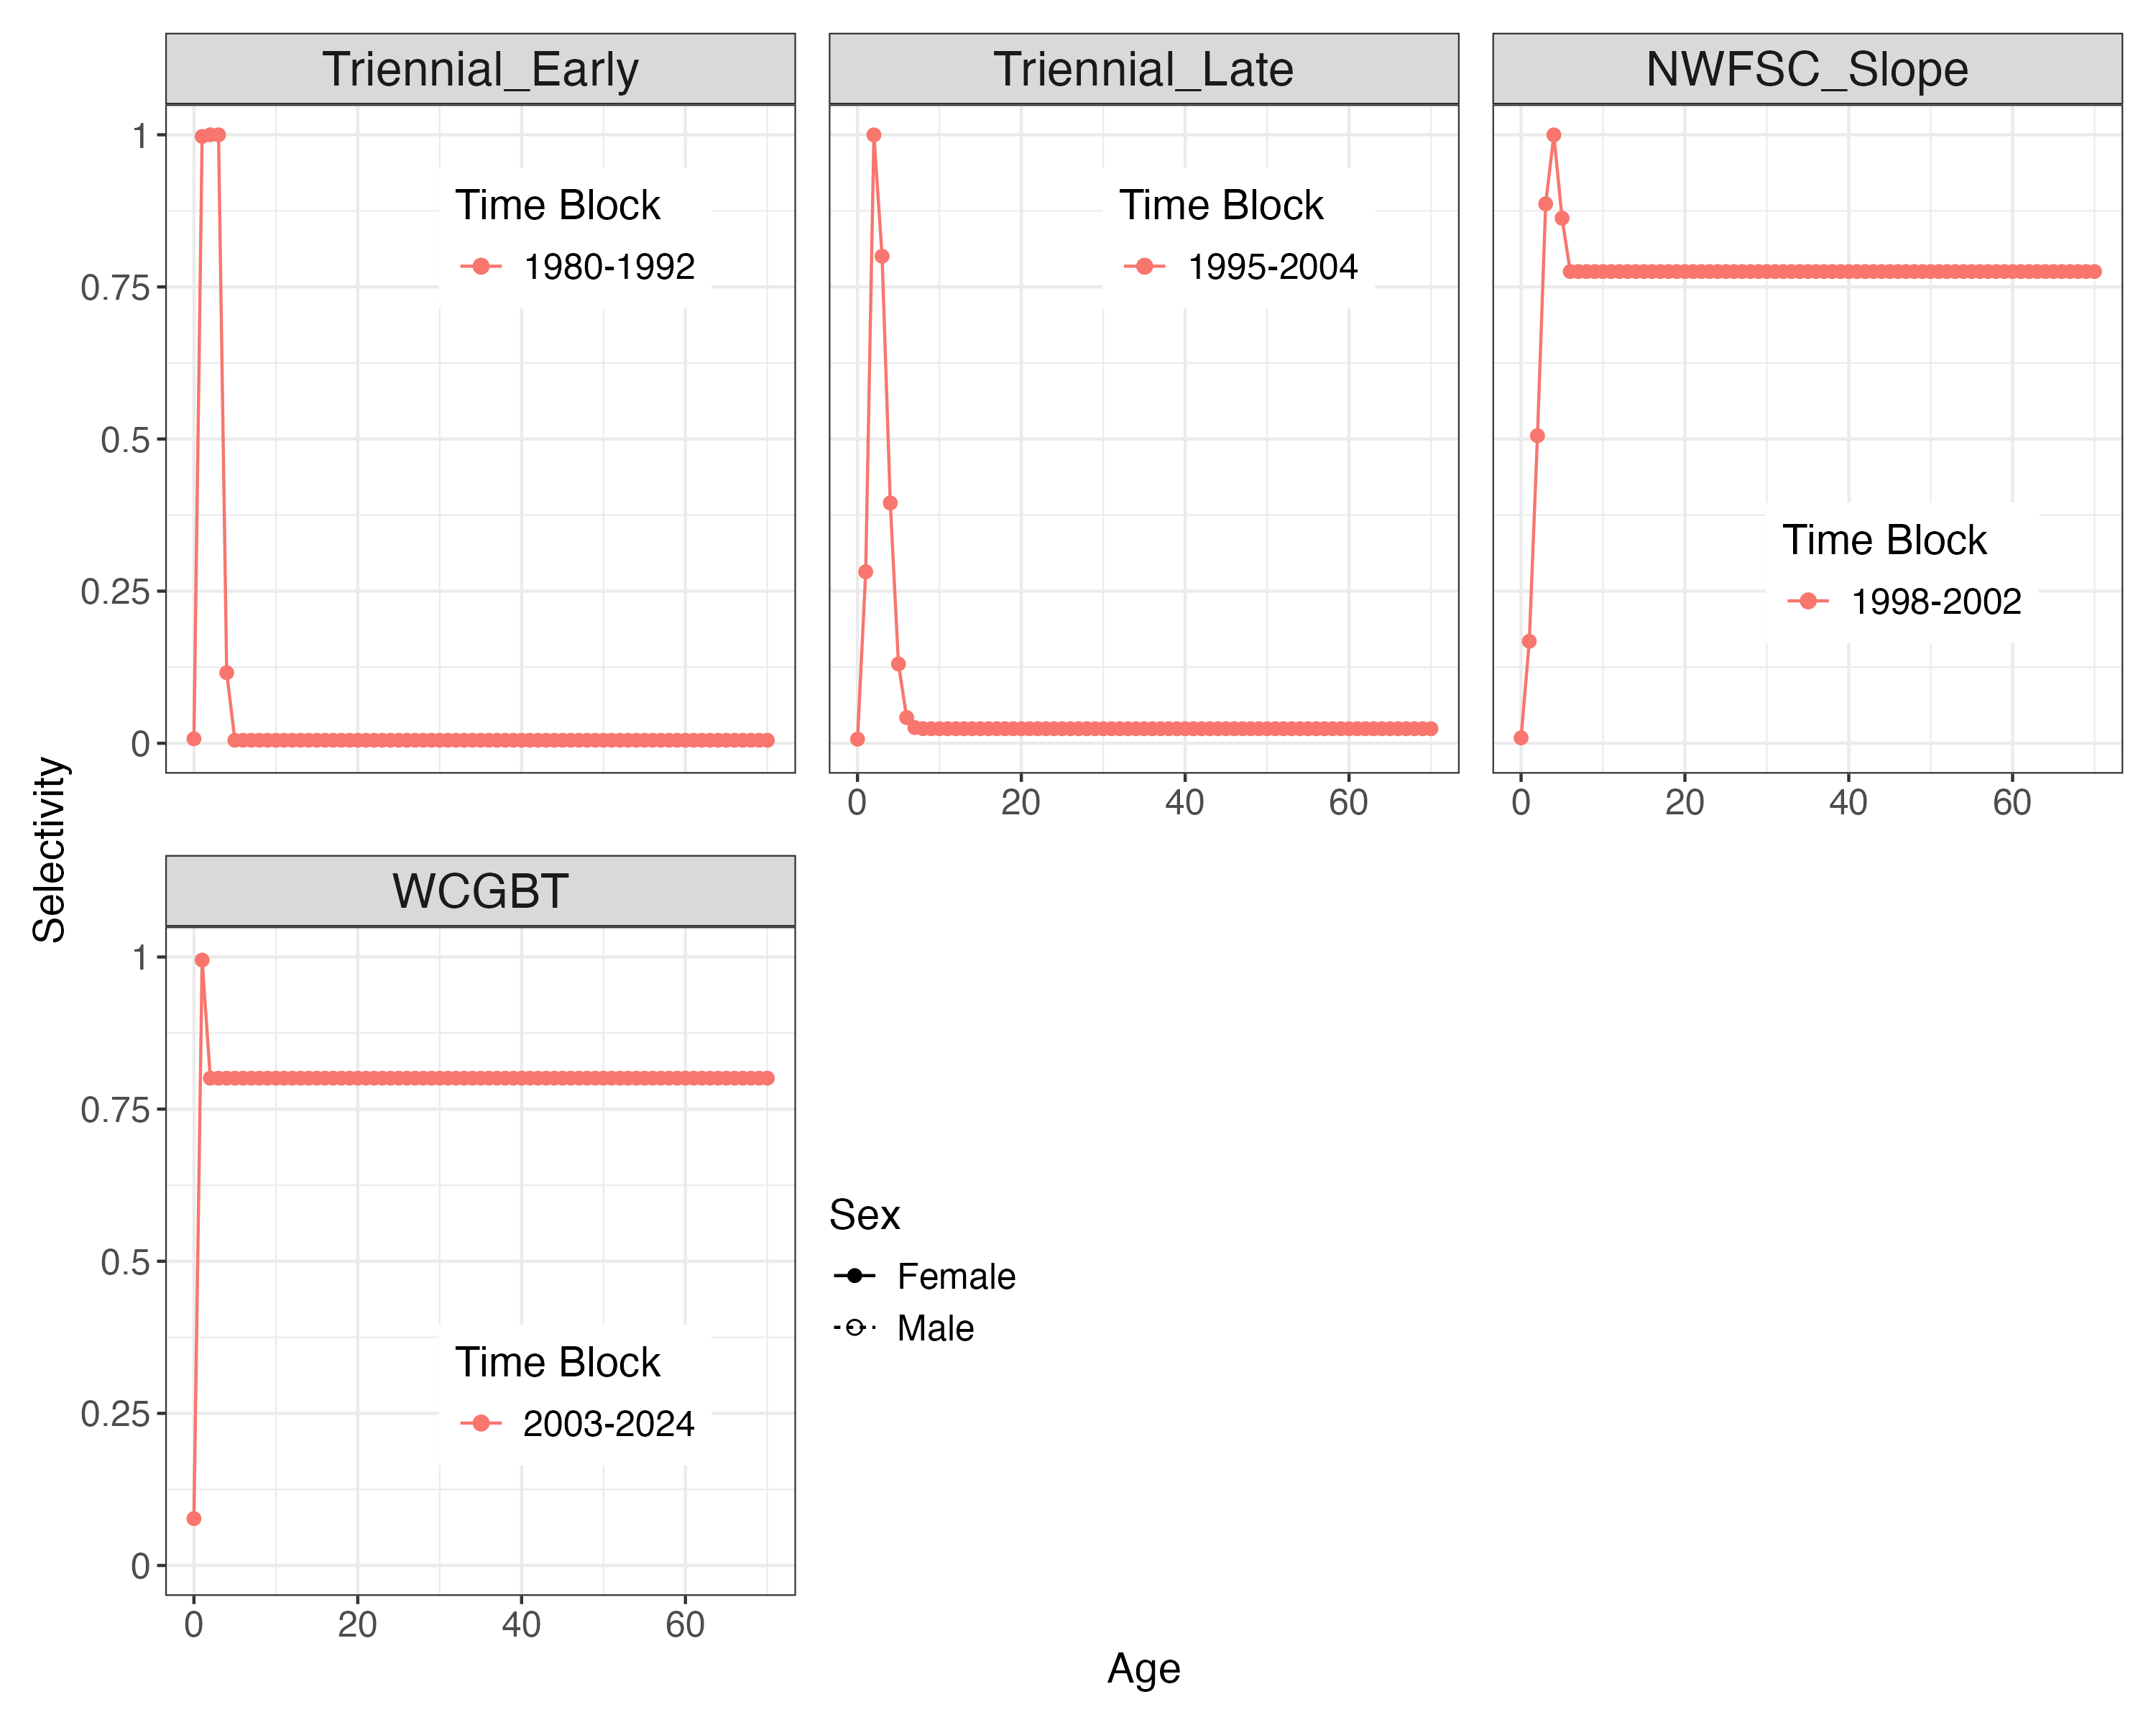
\includegraphics[width=1\linewidth,height=\textheight,keepaspectratio,alt={'Line plot with age in years on the x-axis and selectivity ranging from 0 to 1 on the y-axis with a panel for each survey fleet in the model.  Selectivity for each survey fleet is dome shaped with reduced selectivity for older ages.'}]{figures/survey_selex_timeblocks.png}

}

\caption{\label{fig-survey-selex}Selectivity curves for each survey in
the base model.}

\end{figure}%

\begin{figure}[H]

\centering{

\includegraphics[width=1\linewidth,height=\textheight,keepaspectratio,alt={'Point plot with year on the x-axis and age 0 recruits in 1,000s on the y-axis. The highest estimated recruitment in the time series occurs in 2008, 2013, 2016, 2020, 2021, and 2023.'}]{../model/base_model/8.36_base_model/plots/ts11_Age-0_recruits_(1000s)_with_95_asymptotic_intervals.png}

}

\caption{\label{fig-recruits}Estimated time series of age-0 recruits in
1,000s of fish for the base model.}

\end{figure}%

\pagebreak

\begin{figure}[H]

\centering{

\includegraphics[width=1\linewidth,height=\textheight,keepaspectratio,alt={'Point plot with year on the x-axis and recruitment deviations in log-space along y-axis. The largest positive estimated recruitment deviations in the time series occurs in 2008, 2013, 2016, 2020, 2021, and 2023. The largest negative estimated recruitment deviations in the time series occurs in 1996, 1997, 1998, 2005, 2006, and 2007. See the Report.sso file for estimates.'}]{../model/base_model/8.36_base_model/plots/recdevs2_withbars.png}

}

\caption{\label{fig-recdevs}Estimated time series of recruitment
deviations in log-space for the base model.}

\end{figure}%

\begin{figure}[H]

\centering{

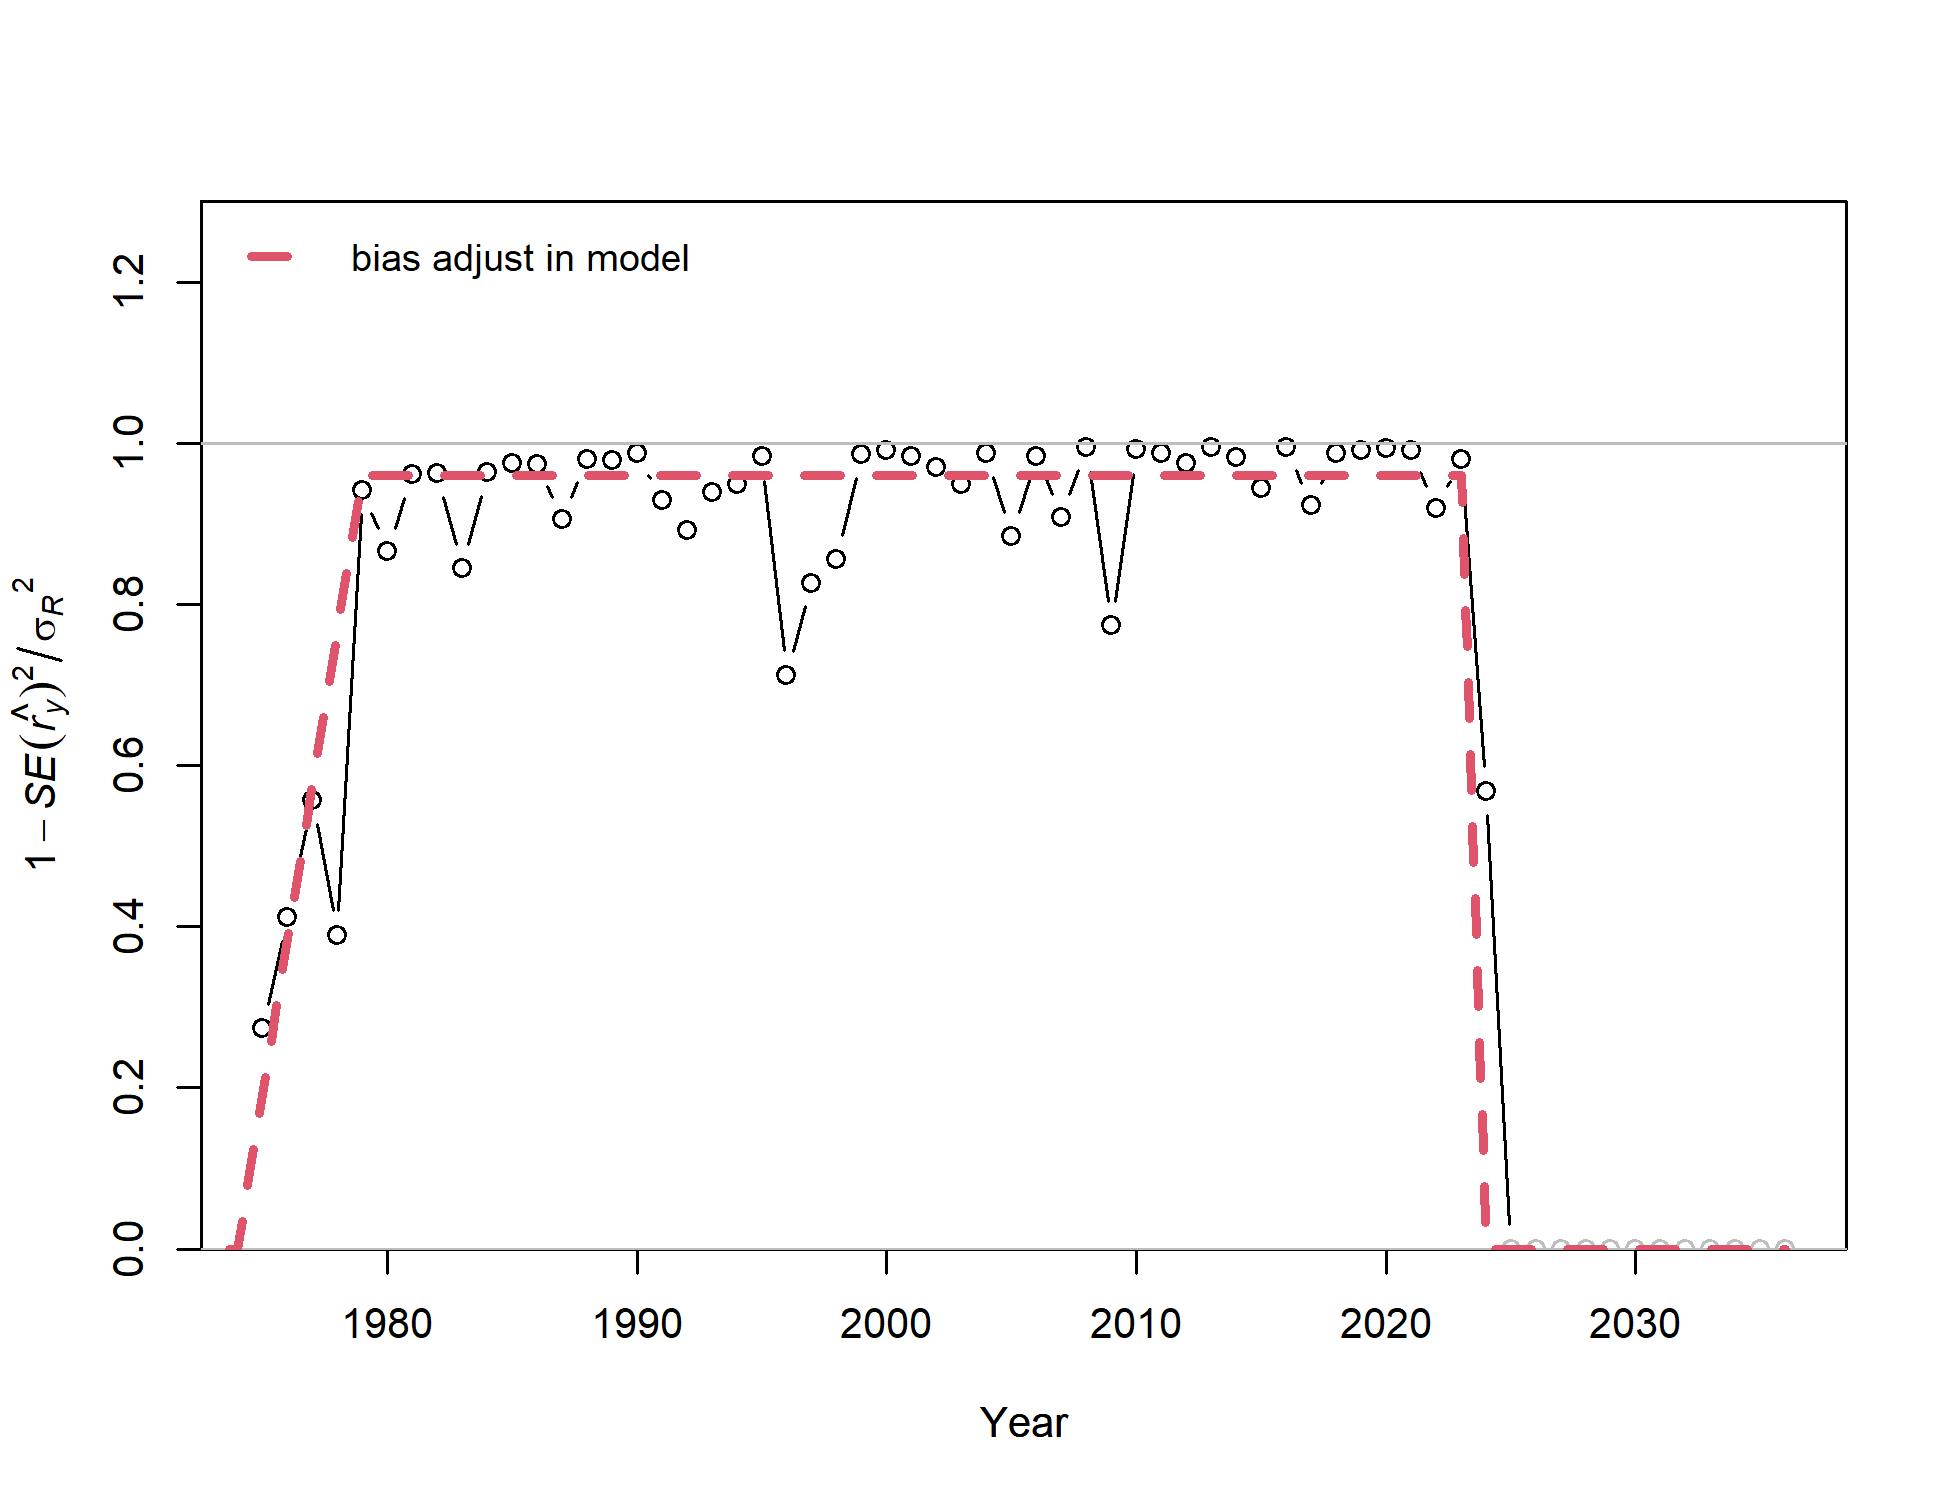
\includegraphics[width=1\linewidth,height=\textheight,keepaspectratio,alt={'Line plot with year on the x-axis and least squares ratio of estimated recruitment variation to sigma R squared. The bias ramp increases linear from 0 to 0.96 between 1974 to 1979. The maximum bias adjustment of 0.96 is applied from 1979 to 2023 and ramps down to 0 bias adjustment starting in 2024.'}]{figures/recruit_fit_bias_adjust.png}

}

\caption{\label{fig-biasramp}Bias adjustment applied to the recruitment
deviations (red line). Points are transformed variances relative to the
assumed variance of recruitment.}

\end{figure}%

\subsection{Fits to Data}\label{fits-to-data}

\begin{figure}[H]

\centering{

\includegraphics[width=1\linewidth,height=\textheight,keepaspectratio,alt={'Line plot with year along the x-axis and relative abundance in metric tons along the y-axis with point and uncertainty intervals show for each year and the model fit.  The model fit to the index data aligned with the index point estimate for 1980 through 1989 and under fit the point estimate in 1992 but was within the uncertainty interval.'}]{../model/base_model/8.36_base_model/plots/index2_cpuefit_Triennial_Early.png}

}

\caption{\label{fig-index-fit-early-triennial}Fit to index data for the
early Triennial Survey (1980-1992).}

\end{figure}%

\begin{figure}[H]

\centering{

\includegraphics[width=1\linewidth,height=\textheight,keepaspectratio,alt={'Line plot with year along the x-axis and relative abundance in metric tons along the y-axis with point and uncertainty intervals show for each year and the model fit. The model fit the the 1995 data point, was greater than the input uncertainty in 1998, lower than the input uncertainty in 2001, and was similar to the point estimate in 2004.'}]{../model/base_model/8.36_base_model/plots/index2_cpuefit_Triennial_Late.png}

}

\caption{\label{fig-index-fit-late-triennial}Fit to index data for the
late Triennial Survey (1995-2004).}

\end{figure}%

\begin{figure}[H]

\centering{

\includegraphics[width=1\linewidth,height=\textheight,keepaspectratio,alt={'Line plot with year along the x-axis and relative abundance in metric tons along the y-axis with point and uncertainty intervals show for each year and the model fit. The model estimate time series was greater than the input uncertainty interval in 1998, within the uncertainty interval in 1999, 2000, and 2001, and below the uncertainty interval in 2002.'}]{../model/base_model/8.36_base_model/plots/index2_cpuefit_NWFSC_Slope.png}

}

\caption{\label{fig-index-fit-nwfsc-slope}Fit to index data for the
NWFSC Slope Survey.}

\end{figure}%

\begin{figure}[H]

\centering{

\includegraphics[width=1\linewidth,height=\textheight,keepaspectratio,alt={'Line plot with year along the x-axis and relative abundance in metric tons along the y-axis with point and uncertainty intervals show for each year and the model fit. The model estimate fit the input uncertainty interval for all years, except 2020 where the model fit was greater than the uncertainty interval and 2022 where the model fit was lower than the input uncertainty interval.'}]{../model/base_model/8.36_base_model/plots/index2_cpuefit_WCGBTS.png}

}

\caption{\label{fig-index-fit-wcgbt}Fit to index data for the NWFSC West
Coast Groundfish Bottom Trawl Survey.}

\end{figure}%

\begin{figure}[H]

\centering{

\includegraphics[width=1\linewidth,height=\textheight,keepaspectratio,alt={'Line plot with year along the x-axis and relative abundance in metric tons along the y-axis with point and uncertainty intervals show for each year and the model fit. The model fit generally followed the trend of the point estimate estimating above average recuitment in 2020, 2021, 2023, and 2024 and below average recruitment in 2022.'}]{../model/base_model/8.36_base_model/plots/index2_cpuefit_Recruitment_Index.png}

}

\caption{\label{fig-index-fit-enviro}Fit to index data for the
recuitment index.}

\end{figure}%

\begin{figure}[H]

\centering{

\includegraphics[width=1\linewidth,height=\textheight,keepaspectratio,alt={'Proportion of ages with age on the x-axis and proportion on the y-axis by sex and unsexed for each fleet in the model and the model fit the proportions by age and sex. The model fit the age proportions by sex generally well for each fleet in the model.'}]{../model/base_model/8.36_base_model/plots/comp_agefit__aggregated_across_time.png}

}

\caption{\label{fig-aggregate-age-fit}Aggregated fit to the age
composition data across all years by fleet.}

\end{figure}%

\begin{figure}[H]

\centering{

\includegraphics[width=1\linewidth,height=\textheight,keepaspectratio,alt={'Plot with year on the x-axis and age in years on the y-axis with circles indicating the Pearson residuals by age and sex for each year with data. There wer no clear patterns in the Pearson residuals and the residuals ranged from -4 to 4.'}]{../model/base_model/8.36_base_model/plots/comp_agefit_residsflt1mkt0_page2.png}

}

\caption{\label{fig-pearson-trawl}Pearsons residuals to age composition
data from the trawl fleet. Closed bubbles are positive residuals
(observed \textgreater{} expected) and open bubbles are negative
residuals (observed \textless{} expected).}

\end{figure}%

\begin{figure}[H]

\centering{

\includegraphics[width=1\linewidth,height=\textheight,keepaspectratio,alt={'Line plot with year along the x-axis and mean age along the y-axis with median values and quantiles shown for each year of data and the model fit to the mean ages. The model fit generally fit the trend in mean ages across years but the model fit was lower then the mean ages for the late 1990s and 2011 through 2014.'}]{../model/base_model/8.36_base_model/plots/comp_agefit_data_weighting_TA1-8_Trawl.png}

}

\caption{\label{fig-mean-age-trawl}Mean age by year with confidence
intervals for sexed and unsexed ages from the trawl fleet. The top panel
is sexed ages and the bottom panel includes both sexed and unsexed
ages.}

\end{figure}%

\begin{figure}[H]

\centering{

\includegraphics[width=1\linewidth,height=\textheight,keepaspectratio,alt={'Plot with year on the x-axis and age in years on the y-axis with circles indicating the Pearson residuals by age and sex for each year with data. There wer no clear patterns in the Pearson residuals and the residuals ranged from -8 to 8.'}]{../model/base_model/8.36_base_model/plots/comp_agefit_residsflt2mkt0_page2.png}

}

\caption{\label{fig-pearson-hkl}Pearsons residuals to age composition
data from the hook-and-line fleet. Closed bubbles are positive residuals
(observed \textgreater{} expected) and open bubbles are negative
residuals (observed \textless{} expected).}

\end{figure}%

\begin{figure}[H]

\centering{

\includegraphics[width=1\linewidth,height=\textheight,keepaspectratio,alt={'Line plot with year along the x-axis and mean age along the y-axis with median values and quantiles shown for each year of data and the model fit to the mean ages. The model fit generally followed the trend of the mean ages.'}]{../model/base_model/8.36_base_model/plots/comp_agefit_data_weighting_TA1-8_Hook_and_Line.png}

}

\caption{\label{fig-mean-age-hkl}Mean age by year with confidence
intervals for sexed and unsexed ages from the hook-and-line fleet.}

\end{figure}%

\begin{figure}[H]

\centering{

\includegraphics[width=1\linewidth,height=\textheight,keepaspectratio,alt={'Plot with year on the x-axis and age in years on the y-axis with circles indicating the Pearson residuals by age and sex for each year with data. There wer no clear patterns in the Pearson residuals and the residuals ranged from -2 to 2.'}]{../model/base_model/8.36_base_model/plots/comp_agefit_residsflt3mkt0_page2.png}

}

\caption{\label{fig-pearson-pot}Pearsons residuals to age composition
data from the pot fleet. Closed bubbles are positive residuals (observed
\textgreater{} expected) and open bubbles are negative residuals
(observed \textless{} expected).}

\end{figure}%

\begin{figure}[H]

\centering{

\includegraphics[width=1\linewidth,height=\textheight,keepaspectratio,alt={'Line plot with year along the x-axis and mean age along the y-axis with median values and quantiles shown for each year of data and the model fit to the mean ages. The model fit generally followed the trend of the mean ages.'}]{../model/base_model/8.36_base_model/plots/comp_agefit_data_weighting_TA1-8_Pot.png}

}

\caption{\label{fig-mean-age-pot}Mean age by year with confidence
intervals for sexed and unsexed ages from the pot fleet.}

\end{figure}%

\begin{figure}[H]

\centering{

\includegraphics[width=1\linewidth,height=\textheight,keepaspectratio,alt={'Plot with year on the x-axis and age in years on the y-axis with circles indicating the Pearson residuals by age and sex for each year with data. There wer no clear patterns in the Pearson residuals and the residuals ranged from -15 to 15.'}]{../model/base_model/8.36_base_model/plots/comp_agefit_residsflt4mkt0.png}

}

\caption{\label{fig-pearson-trawl-discards}Pearsons residuals to age
composition data from the trawl discard fleet. Closed bubbles are
positive residuals (observed \textgreater{} expected) and open bubbles
are negative residuals (observed \textless{} expected).}

\end{figure}%

\begin{figure}[H]

\centering{

\includegraphics[width=1\linewidth,height=\textheight,keepaspectratio,alt={'Line plot with year along the x-axis and mean age along the y-axis with median values and quantiles shown for each year of data and the model fit to the mean ages. The model fit generally followed the trend of the mean ages.'}]{../model/base_model/8.36_base_model/plots/comp_agefit_data_weighting_TA1-8_Trawl_Discard.png}

}

\caption{\label{fig-mean-age-trawl-discards}Mean age by year with
confidence intervals for sexed and unsexed ages from the trawl discard
fleet.}

\end{figure}%

\begin{figure}[H]

\centering{

\includegraphics[width=1\linewidth,height=\textheight,keepaspectratio,alt={'Plot with year on the x-axis and age in years on the y-axis with circles indicating the Pearson residuals by age for each year with data. There wer no clear patterns in the Pearson residuals and the residuals ranged from -2 to 2.'}]{../model/base_model/8.36_base_model/plots/comp_agefit_residsflt5mkt0.png}

}

\caption{\label{fig-pearson-hkl-discards}Pearsons residuals to age
composition data from the hook-and-line discard fleet. Closed bubbles
are positive residuals (observed \textgreater{} expected) and open
bubbles are negative residuals (observed \textless{} expected).}

\end{figure}%

\begin{figure}[H]

\centering{

\includegraphics[width=1\linewidth,height=\textheight,keepaspectratio,alt={'Line plot with year along the x-axis and mean age along the y-axis with median values and quantiles shown for each year of data and the model fit to the mean ages. The model fit generally followed the trend of the mean ages.'}]{../model/base_model/8.36_base_model/plots/comp_agefit_data_weighting_TA1-8_Hook_and_Line_Discard.png}

}

\caption{\label{fig-mean-age-hkl-discards}Mean age by year with
confidence intervals for sexed and unsexed ages from the hook-and-line
discard fleet.}

\end{figure}%

\begin{figure}[H]

\centering{

\includegraphics[width=1\linewidth,height=\textheight,keepaspectratio,alt={'Plot with year on the x-axis and age in years on the y-axis with circles indicating the Pearson residuals by age for each year with data. There wer no clear patterns in the Pearson residuals and the residuals ranged from -25 to 25. The single age year combination with the maximum residual occured in 2006 for age 0.'}]{../model/base_model/8.36_base_model/plots/comp_agefit_residsflt6mkt0.png}

}

\caption{\label{fig-pearson-pot-discards}Pearsons residuals to age
composition data from the pot discard fleet. Closed bubbles are positive
residuals (observed \textgreater{} expected) and open bubbles are
negative residuals (observed \textless{} expected).}

\end{figure}%

\begin{figure}[H]

\centering{

\includegraphics[width=1\linewidth,height=\textheight,keepaspectratio,alt={'Line plot with year along the x-axis and mean age along the y-axis with median values and quantiles shown for each year of data and the model fit to the mean ages. The model fit generally followed the trend of the mean ages.'}]{../model/base_model/8.36_base_model/plots/comp_agefit_data_weighting_TA1-8_Pot_Discard.png}

}

\caption{\label{fig-mean-age-pot-discards}Mean age by year with
confidence intervals for sexed and unsexed ages from the pot discard
fleet.}

\end{figure}%

\begin{figure}[H]

\centering{

\includegraphics[width=1\linewidth,height=\textheight,keepaspectratio,alt={'Plot with year on the x-axis and age in years on the y-axis with circles indicating the Pearson residuals by age and sex for each year with data. There wer no clear patterns in the Pearson residuals and the residuals ranged from -2 to 2.'}]{../model/base_model/8.36_base_model/plots/comp_agefit_residsflt7mkt0.png}

}

\caption{\label{fig-pearson-tri-early}Pearsons residuals to age
composition data from the Triennial Survey (1980-1992). Closed bubbles
are positive residuals (observed \textgreater{} expected) and open
bubbles are negative residuals (observed \textless{} expected).}

\end{figure}%

\begin{figure}[H]

\centering{

\includegraphics[width=1\linewidth,height=\textheight,keepaspectratio,alt={'Line plot with year along the x-axis and mean age along the y-axis with median values and quantiles shown for each year of data and the model fit to the mean ages. The model fit generally followed the trend of the mean ages.'}]{../model/base_model/8.36_base_model/plots/comp_agefit_data_weighting_TA1-8_Triennial_Early.png}

}

\caption{\label{fig-mean-age-tri-early}Mean age by year with confidence
intervals for sexed and unsexed ages from the Triennial Survey
(1980-1992).}

\end{figure}%

\begin{figure}[H]

\centering{

\includegraphics[width=1\linewidth,height=\textheight,keepaspectratio,alt={'Plot with year on the x-axis and age in years on the y-axis with circles indicating the Pearson residuals by age and sex for each year with data. There wer no clear patterns in the Pearson residuals and the residuals ranged from -4 to 4.'}]{../model/base_model/8.36_base_model/plots/comp_agefit_residsflt8mkt0.png}

}

\caption{\label{fig-pearson-tri-late}Pearsons residuals to age
composition data from the Triennial Survey (1995-2004). Closed bubbles
are positive residuals (observed \textgreater{} expected) and open
bubbles are negative residuals (observed \textless{} expected).}

\end{figure}%

\begin{figure}[H]

\centering{

\includegraphics[width=1\linewidth,height=\textheight,keepaspectratio,alt={'Line plot with year along the x-axis and mean age along the y-axis with median values and quantiles shown for each year of data and the model fit to the mean ages. The model fit generally followed the trend of the mean ages.'}]{../model/base_model/8.36_base_model/plots/comp_agefit_data_weighting_TA1-8_Triennial_Late.png}

}

\caption{\label{fig-mean-age-tri-late}Mean age by year with confidence
intervals for sexed and unsexed ages from the Triennial Survey
(1995-2004).}

\end{figure}%

\begin{figure}[H]

\centering{

\includegraphics[width=1\linewidth,height=\textheight,keepaspectratio,alt={'Plot with year on the x-axis and age in years on the y-axis with circles indicating the Pearson residuals by age and sex for each year with data. There wer no clear patterns in the Pearson residuals and the residuals ranged from -2 to 2.'}]{../model/base_model/8.36_base_model/plots/comp_agefit_residsflt9mkt0.png}

}

\caption{\label{fig-pearson-nwfsc-slope}Pearsons residuals to age
composition data from the NWFSC Slope Survey. Closed bubbles are
positive residuals (observed \textgreater{} expected) and open bubbles
are negative residuals (observed \textless{} expected).}

\end{figure}%

\begin{figure}[H]

\centering{

\includegraphics[width=1\linewidth,height=\textheight,keepaspectratio,alt={'Line plot with year along the x-axis and mean age along the y-axis with median values and quantiles shown for each year of data and the model fit to the mean ages. The model fit generally followed the trend of the mean ages.'}]{../model/base_model/8.36_base_model/plots/comp_agefit_data_weighting_TA1-8_NWFSC_Slope.png}

}

\caption{\label{fig-mean-age-nwfsc-slope}Mean age by year with
confidence intervals for sexed and unsexed ages from the NWFSC Slope
Survey.}

\end{figure}%

\begin{figure}[H]

\centering{

\includegraphics[width=1\linewidth,height=\textheight,keepaspectratio,alt={'Plot with year on the x-axis and age in years on the y-axis with circles indicating the Pearson residuals by age and sex for each year with data. There wer no clear patterns in the Pearson residuals and the residuals ranged from -10 to 10.'}]{../model/base_model/8.36_base_model/plots/comp_agefit_residsflt10mkt0.png}

}

\caption{\label{fig-pearson-wcgbt}Pearsons residuals to age composition
data from the NWFSC West Coast Groundfish Bottom Trawl Survey. Closed
bubbles are positive residuals (observed \textgreater{} expected) and
open bubbles are negative residuals (observed \textless{} expected).}

\end{figure}%

\begin{figure}[H]

\centering{

\includegraphics[width=1\linewidth,height=\textheight,keepaspectratio,alt={'Line plot with year along the x-axis and mean age along the y-axis with median values and quantiles shown for each year of data and the model fit to the mean ages. The model fit generally followed the trend of the mean ages.'}]{../model/base_model/8.36_base_model/plots/comp_agefit_data_weighting_TA1-8_WCGBTS.png}

}

\caption{\label{fig-mean-age-wcgbt}Mean age by year with confidence
intervals for sexed and unsexed ages from the NWFSC West Coast
Groundfish Bottom Trawl Survey. The top panel is sexed ages and the
bottom panel includes both sexed and unsexed ages.}

\end{figure}%

\subsection{Time-series}\label{time-series}

\begin{figure}[H]

\centering{

\includegraphics[width=1\linewidth,height=\textheight,keepaspectratio,alt={'Line plot with year on the x-axis ranging from 1890 through 2025 and spawning output on the y-axis. In 1890 spawning output is 219,377 metric tons and slowly decreases through 1975 to 178,570 metric tons, sharply decreased between 1976 to 2013 to 22,914 metric tons and slowly increases through 2025 to 74,409 metric tons.  The yearly values are available in Table 31.'}]{../model/base_model/8.36_base_model/plots/ts7_Spawning_output_with_95_intervals.png}

}

\caption{\label{fig-sb}Estimated time series of spawning output for the
base model.}

\end{figure}%

\begin{figure}[H]

\centering{

\includegraphics[width=1\linewidth,height=\textheight,keepaspectratio,alt={'Line plot with year on the x-axis ranging from 1890 through 2025 and age 3 plus biomass on the y-axis. In 1890 age 3 plus biomass is 458,861 metric tons and slowly decreases through 1975 to 391,573 metric tons, sharply decreased between 1976 to 2010 to 70,824 metric tons, remains low from 2011 to 2015, and sharply increases through 2025 to 246,677 metric tons.  The yearly values are available in Table 31.'}]{../model/base_model/8.36_base_model/plots/ts4_Summary_biomass_(t).png}

}

\caption{\label{fig-summary-biomass}Estimated time series of summary
biomass for age 3 and older for the base model.}

\end{figure}%

\begin{figure}[H]

\centering{

\includegraphics[width=1\linewidth,height=\textheight,keepaspectratio,alt={'Line plot with year on the x-axis ranging from 1890 through 2025 and total on the y-axis. In 1890 total biomass is 489,494 metric tons and slowly decreases through 1975 to 422,649 metric tons, sharply decreased between 1976 to 2013 to 91,633 metric tons, and sharply increases through 2025 to 318,750 metric tons. The yearly values are available in Table 31.'}]{../model/base_model/8.36_base_model/plots/ts1_Total_biomass_(t).png}

}

\caption{\label{fig-total-biomass}Estimated time series of total biomass
for the base model.}

\end{figure}%

\begin{figure}[H]

\centering{

\includegraphics[width=1\linewidth,height=\textheight,keepaspectratio,alt={'Line plot with year on the x-axis ranging from 1890 through 2025 and stock status on the y-axis ranging from 0 to 1. Stock status slowly decreases from 1890 to 1975 to 0.814 of unfished, sharply decreased between 1976 to 2013 to 0.104, and slowly increases through 2025 to 0.339 of unfished.  The yearly values are available in Table 31.'}]{../model/base_model/8.36_base_model/plots/ts9_Fraction_of_unfished_spawning_output.png}

}

\caption{\label{fig-depl}Estimated time series of fraction of unfished
spawning output (i.e., stock status) for the base model.}

\end{figure}%

\begin{figure}[H]

\centering{

\includegraphics[width=1\linewidth,height=\textheight,keepaspectratio,alt={'Plot of yearly data points with spawning output on the x-axis and recruitment in 1,000s of fish on the y-axis. The estimated recruitment and spawning output for each year is plotted as point around the assumed Beverton-Holt stock-recruitment curve for a steepness of 0.75. The yearly values for spawning output and recruitment are available in Table 31.'}]{../model/base_model/8.36_base_model/plots/SR_curve2.png}

}

\caption{\label{fig-sb-recr}Stock-recruit curve with labels on first,
last, and years with (log) deviations \textgreater{} 0.5. Point colors
indicate year, with warmer colors indicating earlier years and cooler
colors in showing later years.}

\end{figure}%

\begin{figure}[H]

\centering{

\includegraphics[width=1\linewidth,height=\textheight,keepaspectratio,alt={'Line plot with year from 1890 through 2025 on the x-axis and spawning output on the y-axis. The spawning output trajectory without fishing declines from 1985 to 2020 to approximately 100,000 metric tons given deviations in recruitment alone.  The trajectory then increases in recent years due to above average recruitment to approximately 180,000 metric tons.'}]{../model/base_model/8.36_base_model/plots/ts_DynamicB0.png}

}

\caption{\label{fig-dyn-b0}The lower line shows the time series of
estimated spawning output in the presence of fishing mortality. The
upper line shows the time series that could occur under the same
dynamics (including deviations in recruitment), but without fishing. The
point at the left represents the unfished equilibrium.}

\end{figure}%

\subsection{Sensitivity Analyses}\label{sensitivity-analyses}

\begin{figure}[H]

\centering{

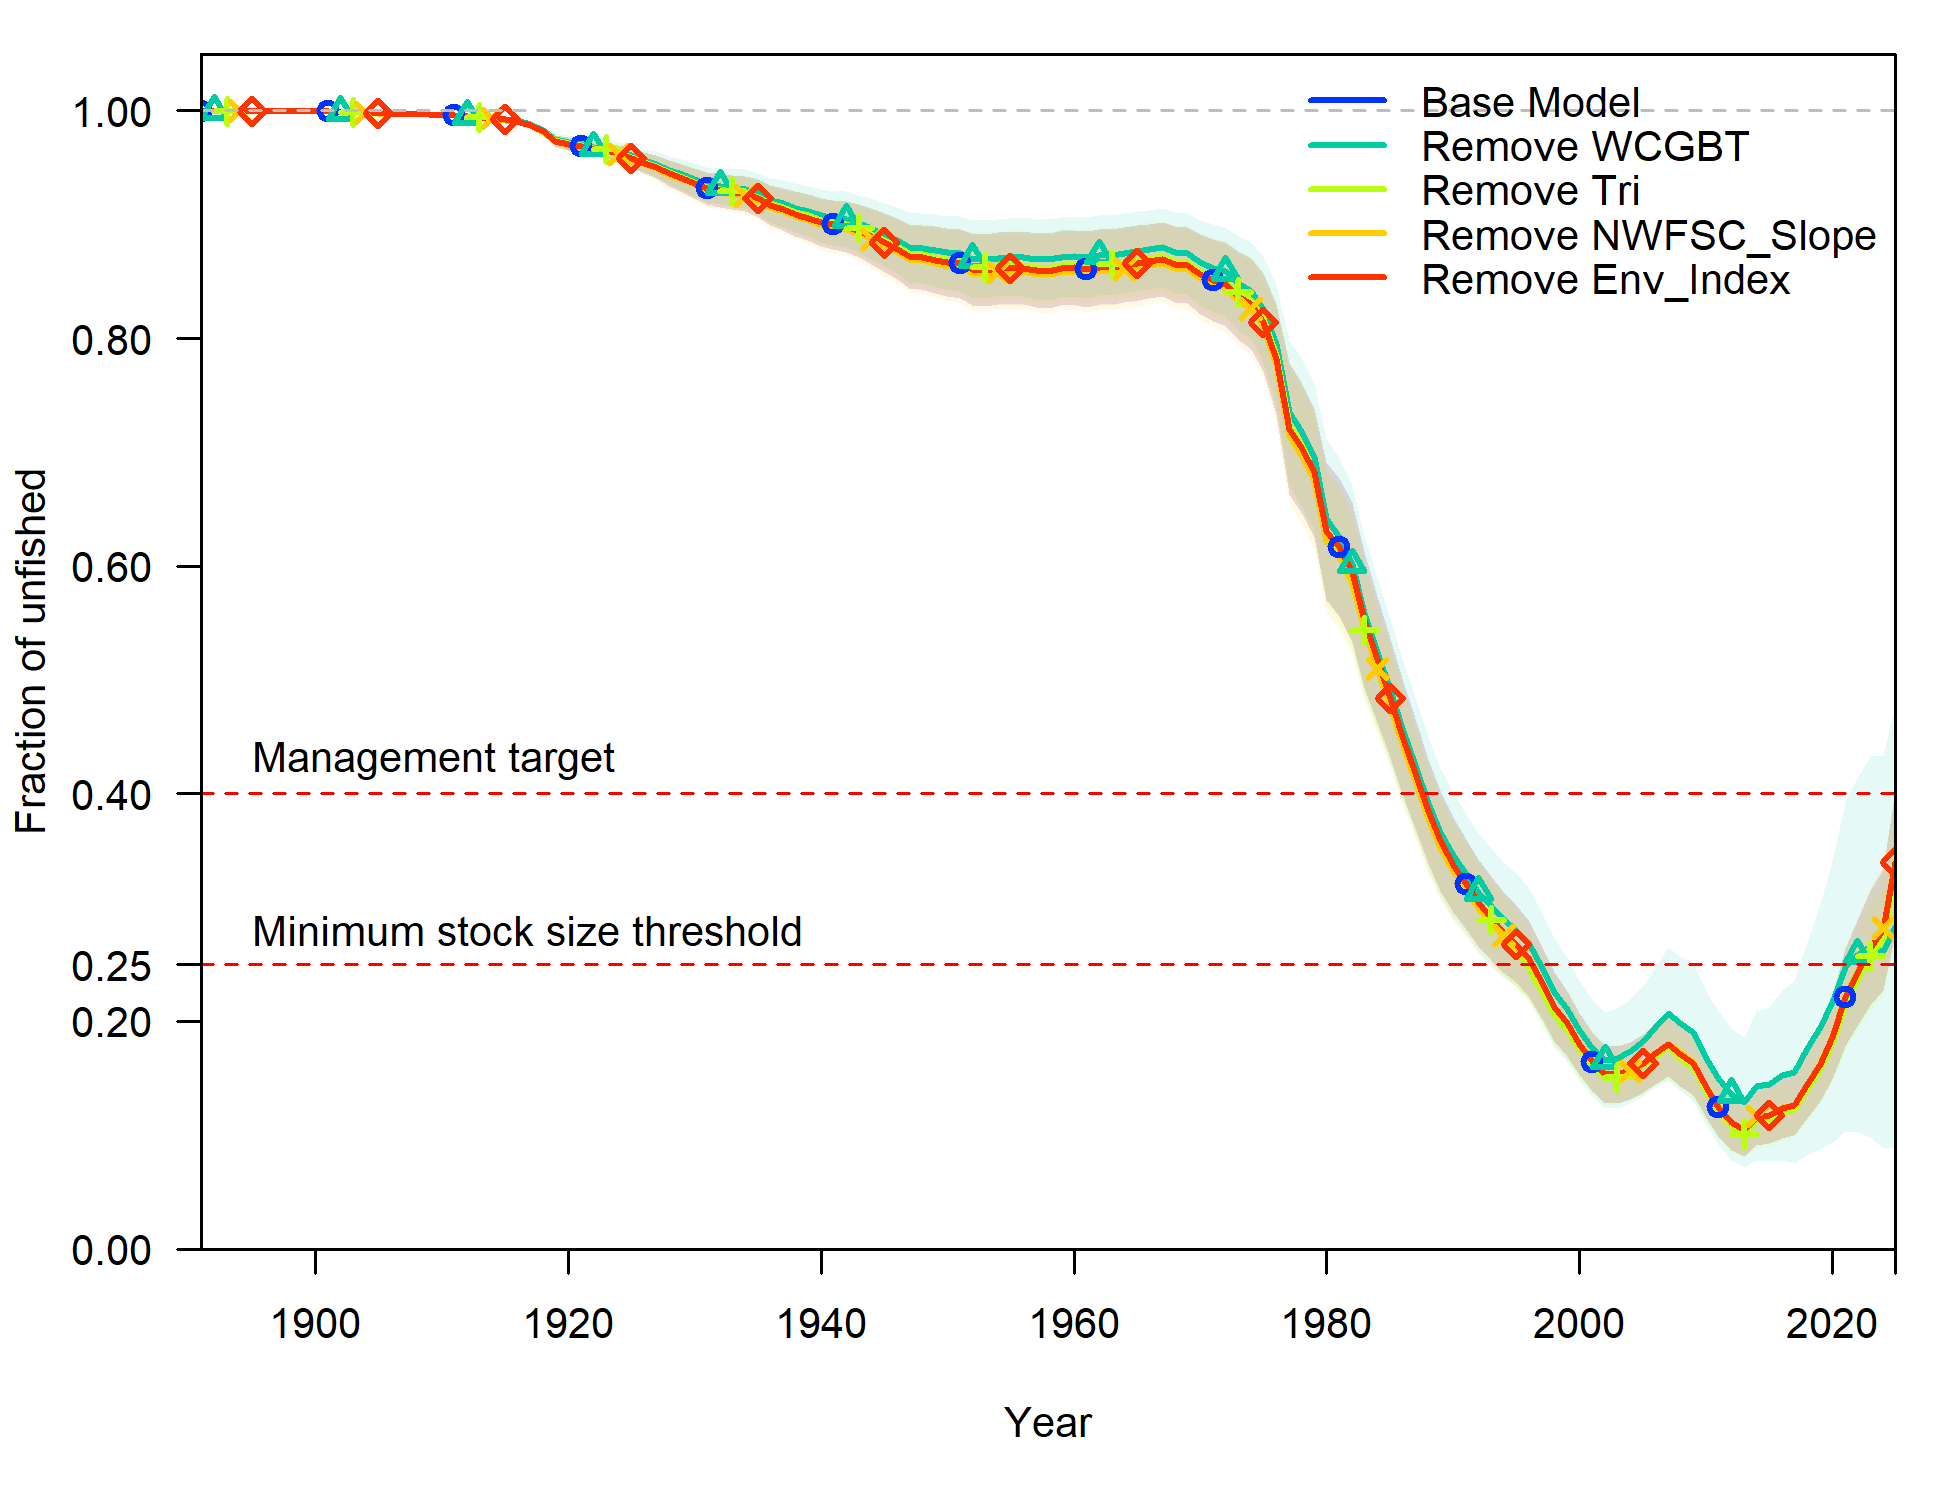
\includegraphics[width=1\linewidth,height=\textheight,keepaspectratio,alt={'Line plot with year on the x-axis and fraction of unfished on the y-axis.  In general, all the sensitivities shown have similar trajectories for fraction of unfished, except for the sensitivity that removes the WCGBTS data where the fraction of unfished is marginally higher than the base model from 2000 throu 2022 and in 2024 is more depleted than the base model. Select parameters and derived quanties are provided in Table 32.'}]{figures/sens_1_compare4_Bratio_uncertainty.png}

}

\caption{\label{fig-sens-1-bratio}Maximum likelihood estimates of
fraction of unfished (i.e., stock status) for the base model and
alternative sensitivity runs representing the removal of index and age
composition data from the West Coast Groundfish Bottom Trawl Survey
(WCGBT), the Trienniel Survey, or the Northwest Fisheries Science Center
Slope Survey. Additionally, estimates for the removal of the
environmental-based recruitment index are shown. Shaded regions
represent asymptotic 95 percent confidence intervals.}

\end{figure}%

\begin{figure}[H]

\centering{

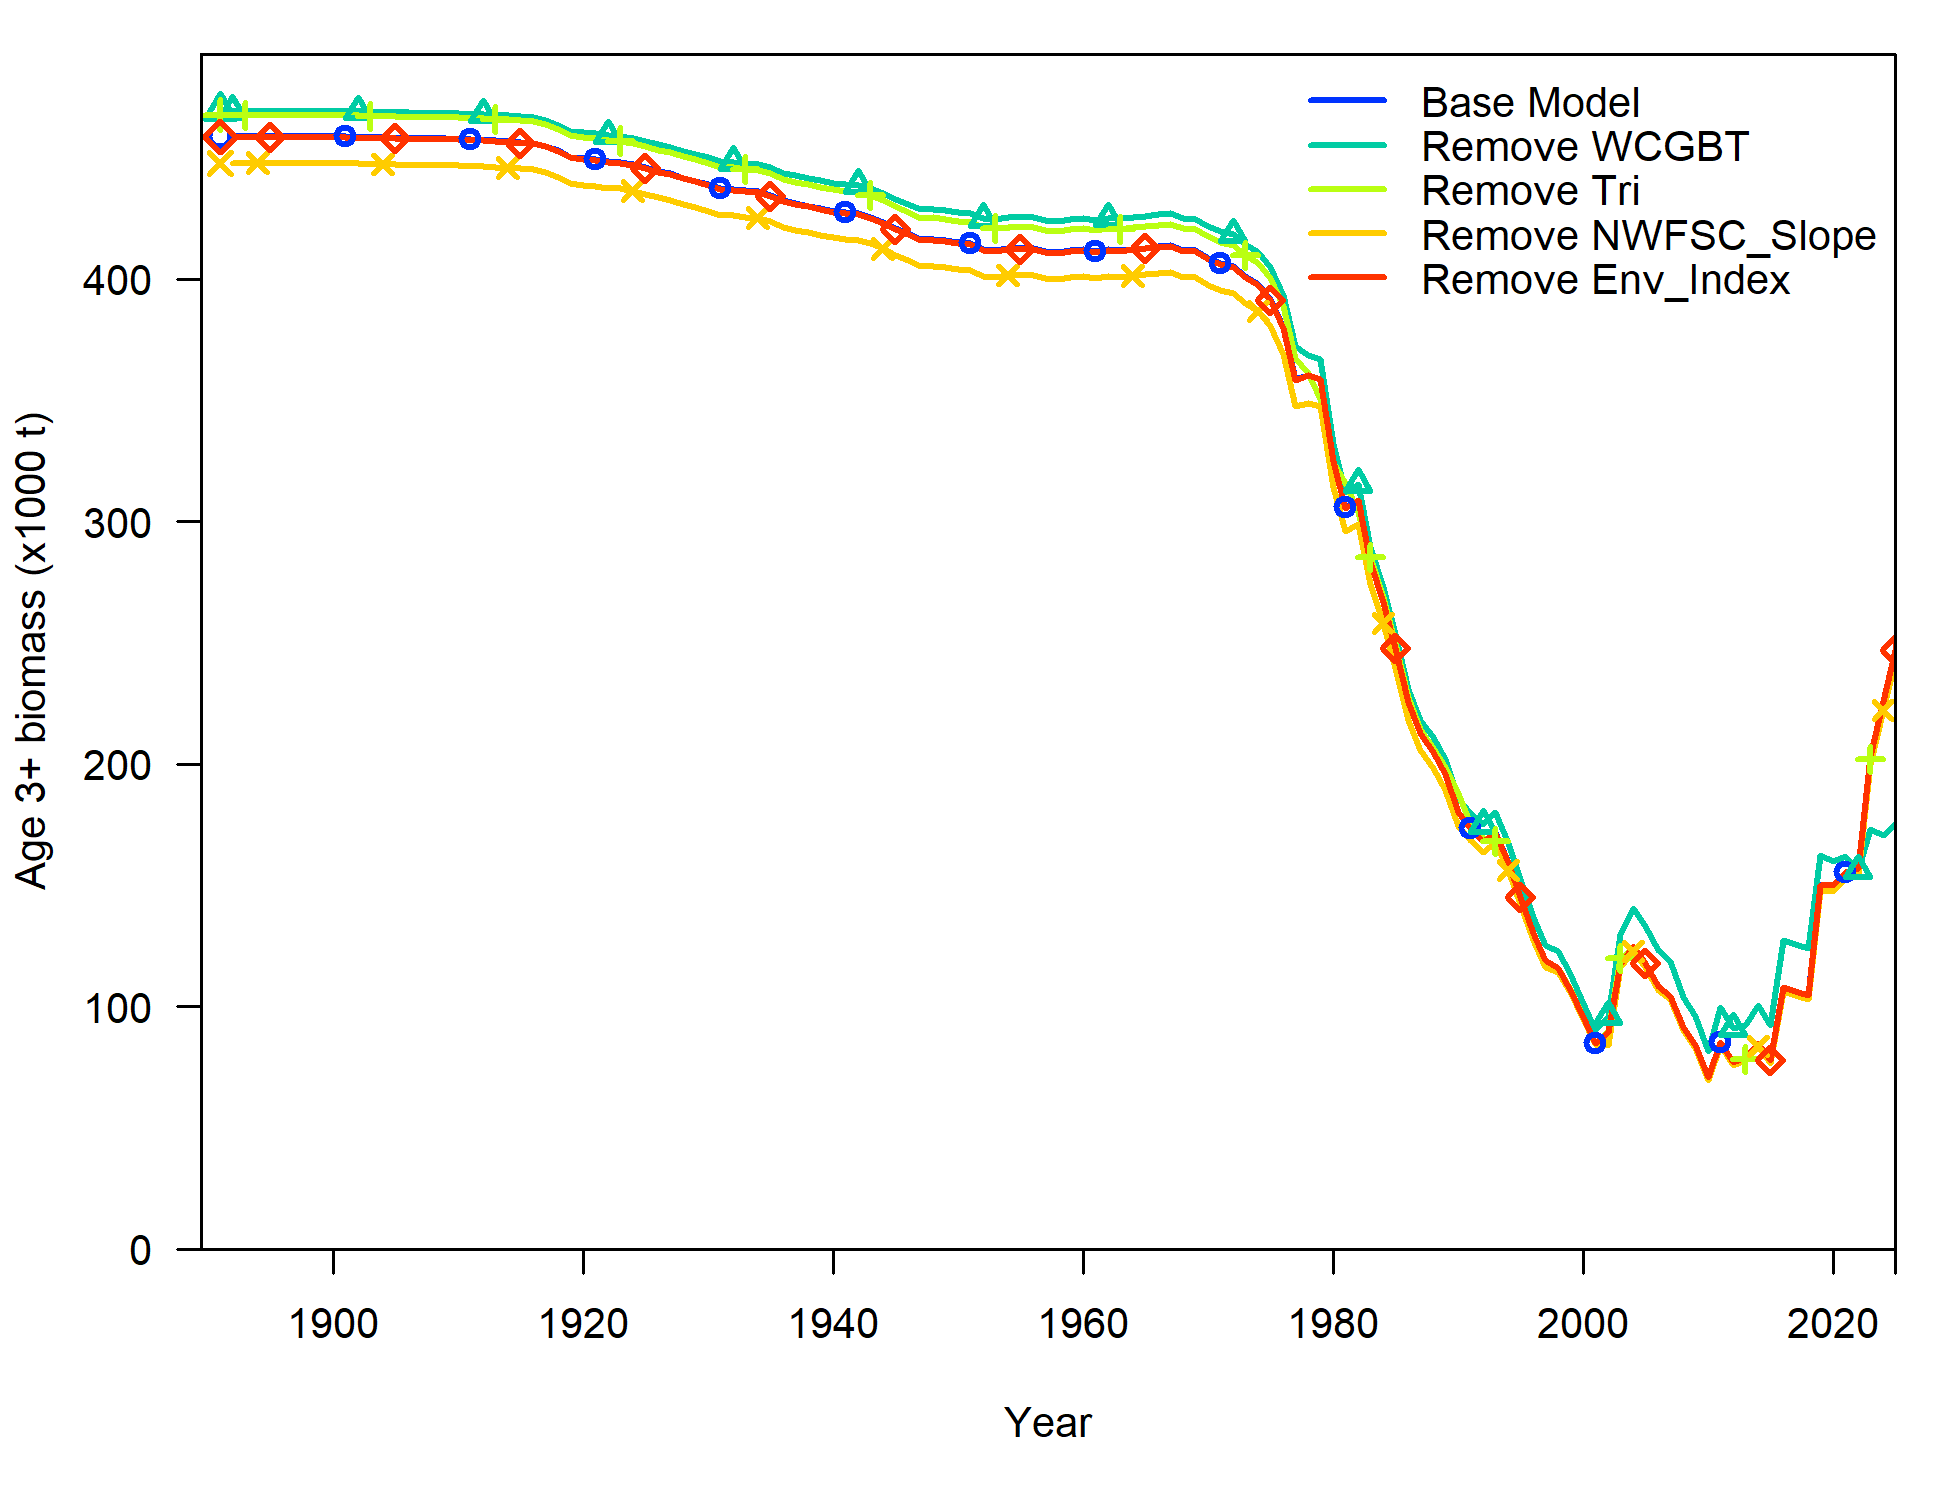
\includegraphics[width=1\linewidth,height=\textheight,keepaspectratio,alt={'Line plot with year on the x-axis and age 3 plus biomass on the y-axis.  In general, all the sensitivities shown have similar trajectories for age 3 plus biomass, except for the sensitivity that removes the WCGBTS data where the age 3 plus biomass at the end of the model is lower than the base model. Select parameters and derived quanties are provided in Table 32.'}]{figures/sens_1_compare18_smrybio.png}

}

\caption{\label{fig-sens-1-sumB}Maximum likelihood estimates of summary
biomass (age 3 and older) for the base model and alternative sensitivity
runs representing the removal of index and age composition data from the
West Coast Groundfish Bottom Trawl Survey (WCGBT), the Trienniel Survey,
or the Northwest Fisheries Science Center Slope Survey. Additionally,
estimates for the removal of the environmental-based recruitment index
are shown.}

\end{figure}%

\begin{figure}[H]

\centering{

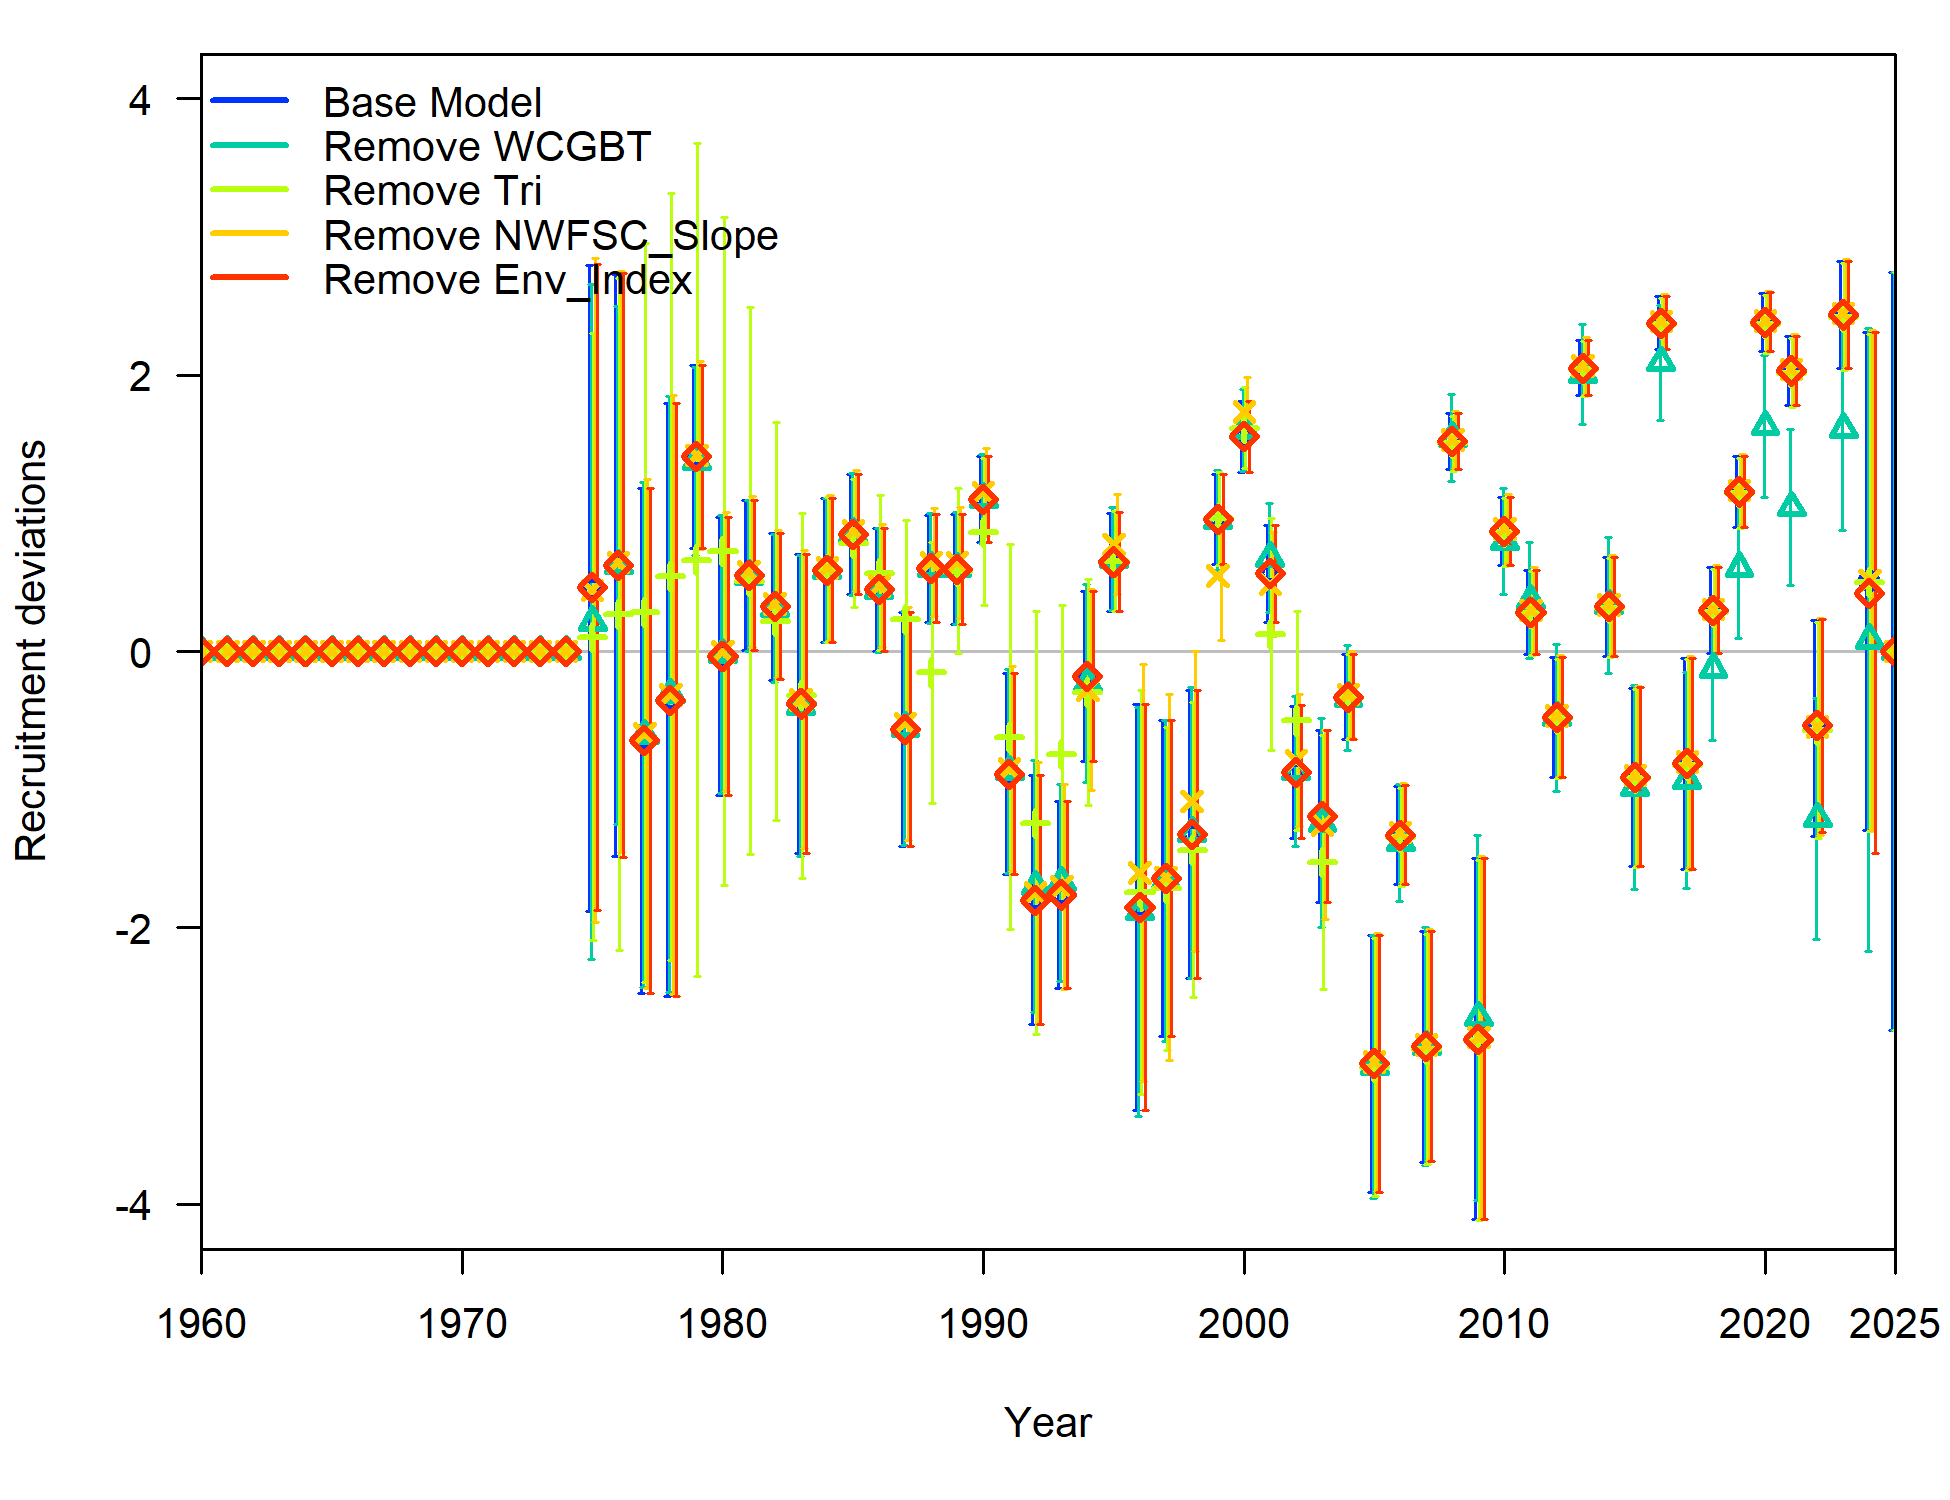
\includegraphics[width=1\linewidth,height=\textheight,keepaspectratio,alt={'Line plot with year on the x-axis and annual recruitment deviations in log-space on the y-axis.  In general, all the sensitivities shown have similar estimates of annual recruitment deviationss, except for the sensitivity that removes the WCGBTS data where the annual recruitment deviations from 2015 through 2024 are less positive or more negative. Select parameters and derived quanties are provided in Table 32.'}]{figures/sens_1_compare12_recdevs_uncertainty.png}

}

\caption{\label{fig-sens-1-recdev}Maximum likelihood estimates of
recruitment deviations from 1960-2025 for the base model and alternative
sensitivity runs representing the removal of index and age composition
data from the West Coast Groundfish Bottom Trawl Survey (WCGBT), the
Trienniel Survey, or the Northwest Fisheries Science Center Slope
Survey. Additionally, estimates for the removal of the
environmental-based recruitment index are shown. Bars represent
asymptotic 95 percent confidence intervals.}

\end{figure}%

\begin{figure}[H]

\centering{

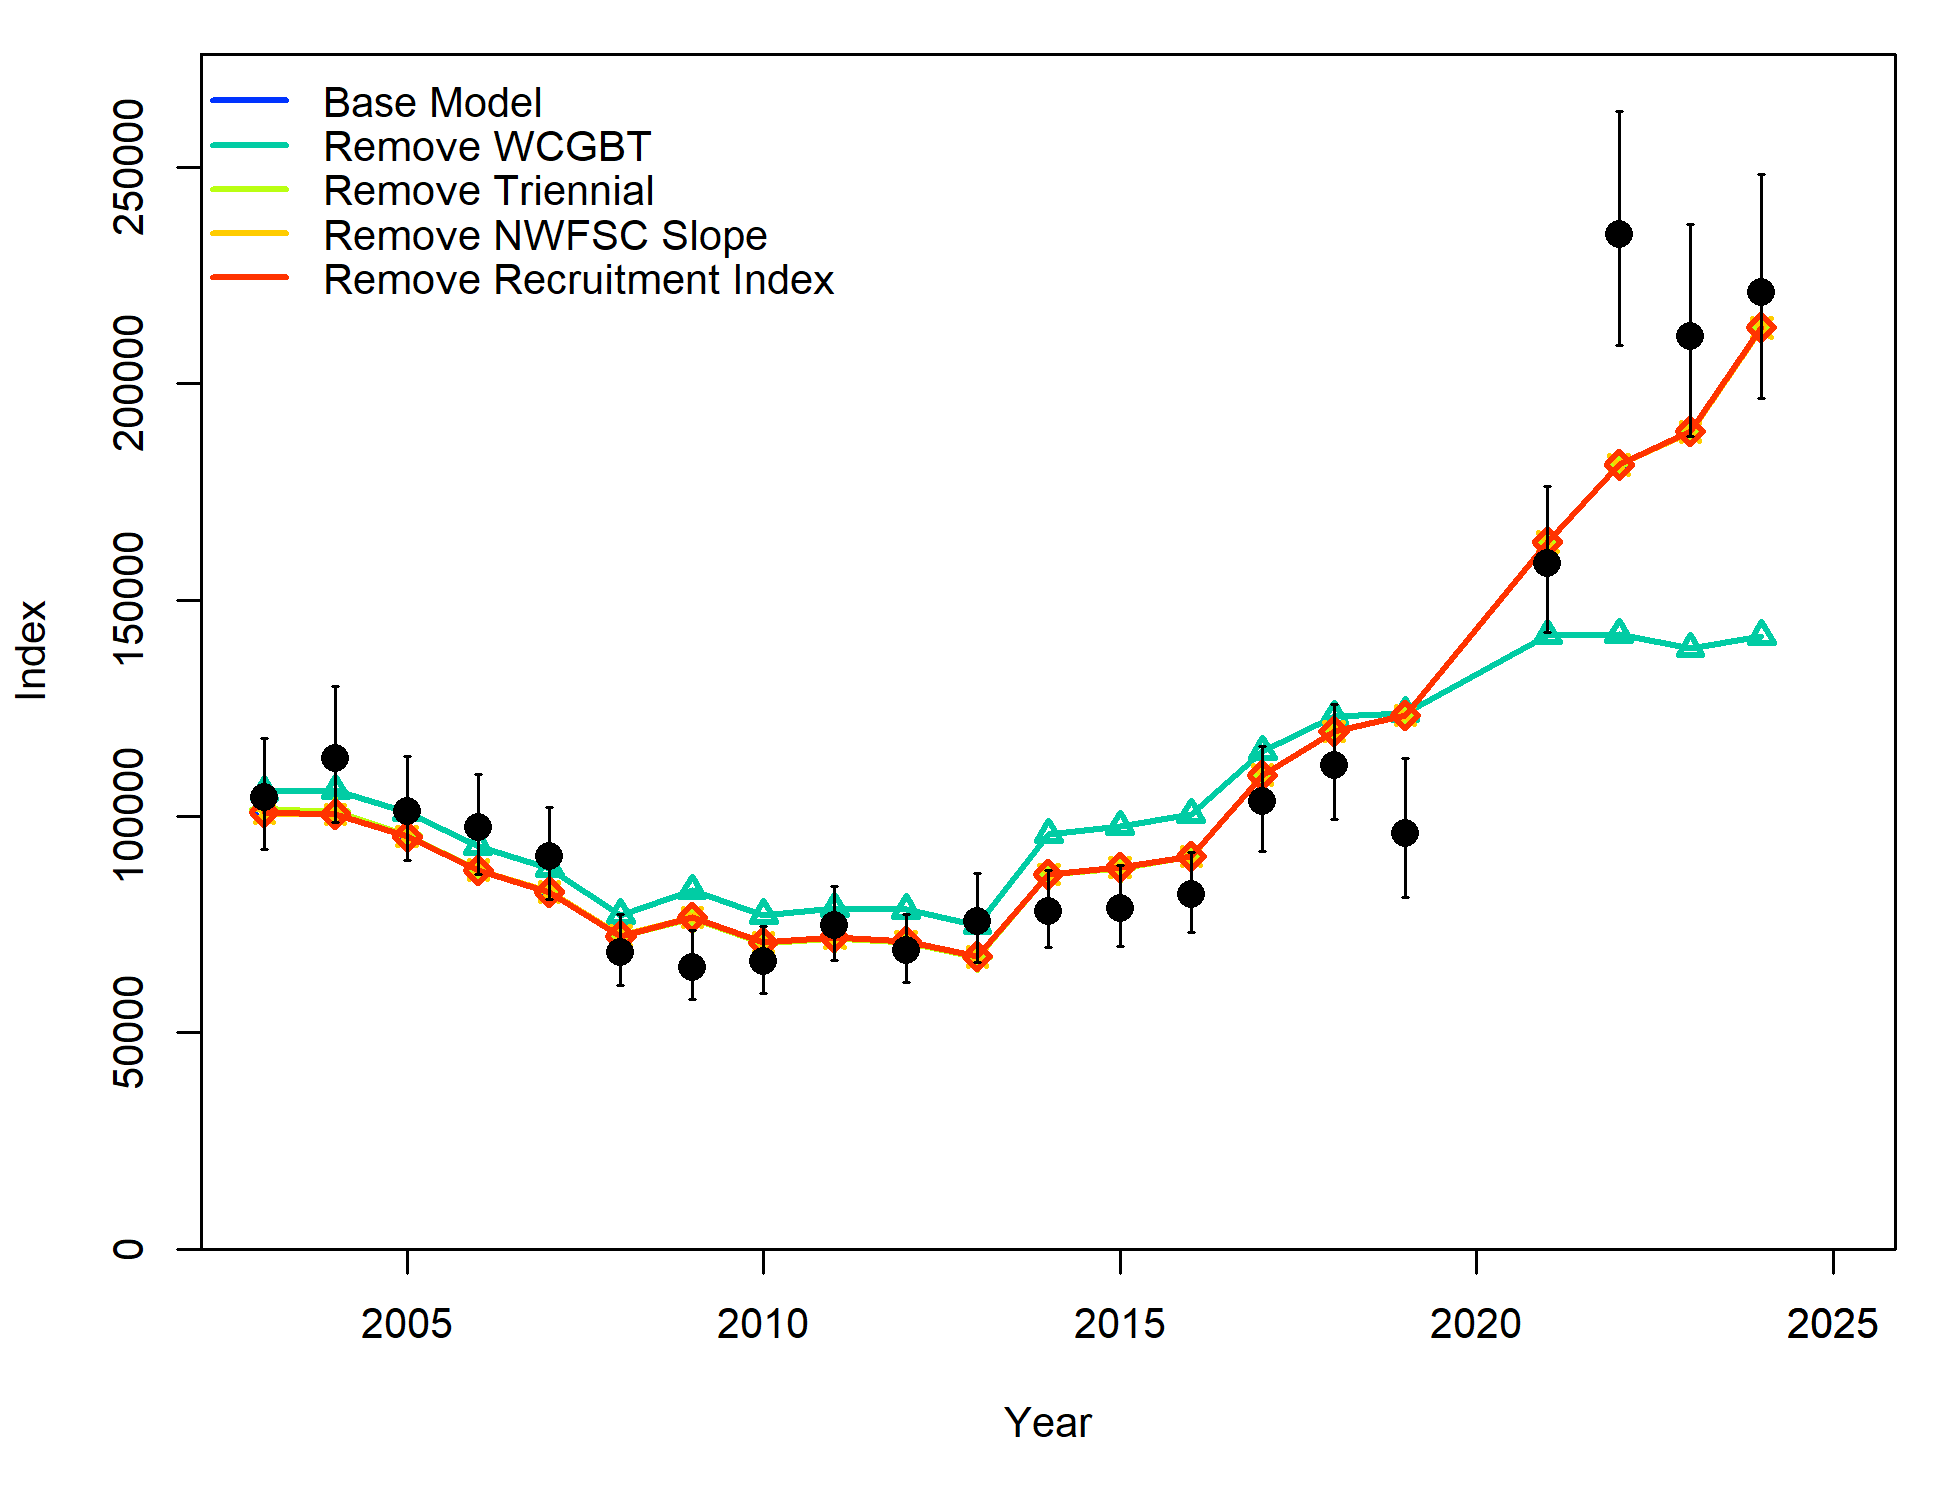
\includegraphics[width=1\linewidth,height=\textheight,keepaspectratio,alt={'Line plot with year on the x-axis from 2003 to 2024 and the relative index and fit to the index from the WCGBTS on the y-axis. The implied fit to the WCGBTS when the survey is removed from the model results in the population not increasing from 2021 through 2024 but rather stabilizing. Select parameters and derived quanties are provided in Table 32.'}]{figures/sens_1_compare13_indices.png}

}

\caption{\label{fig-sens-1-wcgbt}Maximum likelihood estimates of the fit
to the NWFSC West Coast Groundfish Bottom Trawl Survey (WCGBTS) time
series for the base model and alternative sensitivity runs representing
the removal of index and age composition data from the West Coast
Groundfish Bottom Trawl Survey (WCGBTS), the Trienniel Survey, or the
NWFSC Slope Survey. Additionally, estimates for the removal of the
environmental-based recruitment index are shown. The black dots with
error bars represent the input index data points with associated
uncertainty, whereas colors reprsent the estimated values for each year
and model. Note that the results for all models are nearly identical,
except for the Remove WCBGTS run.}

\end{figure}%

\begin{figure}[H]

\centering{

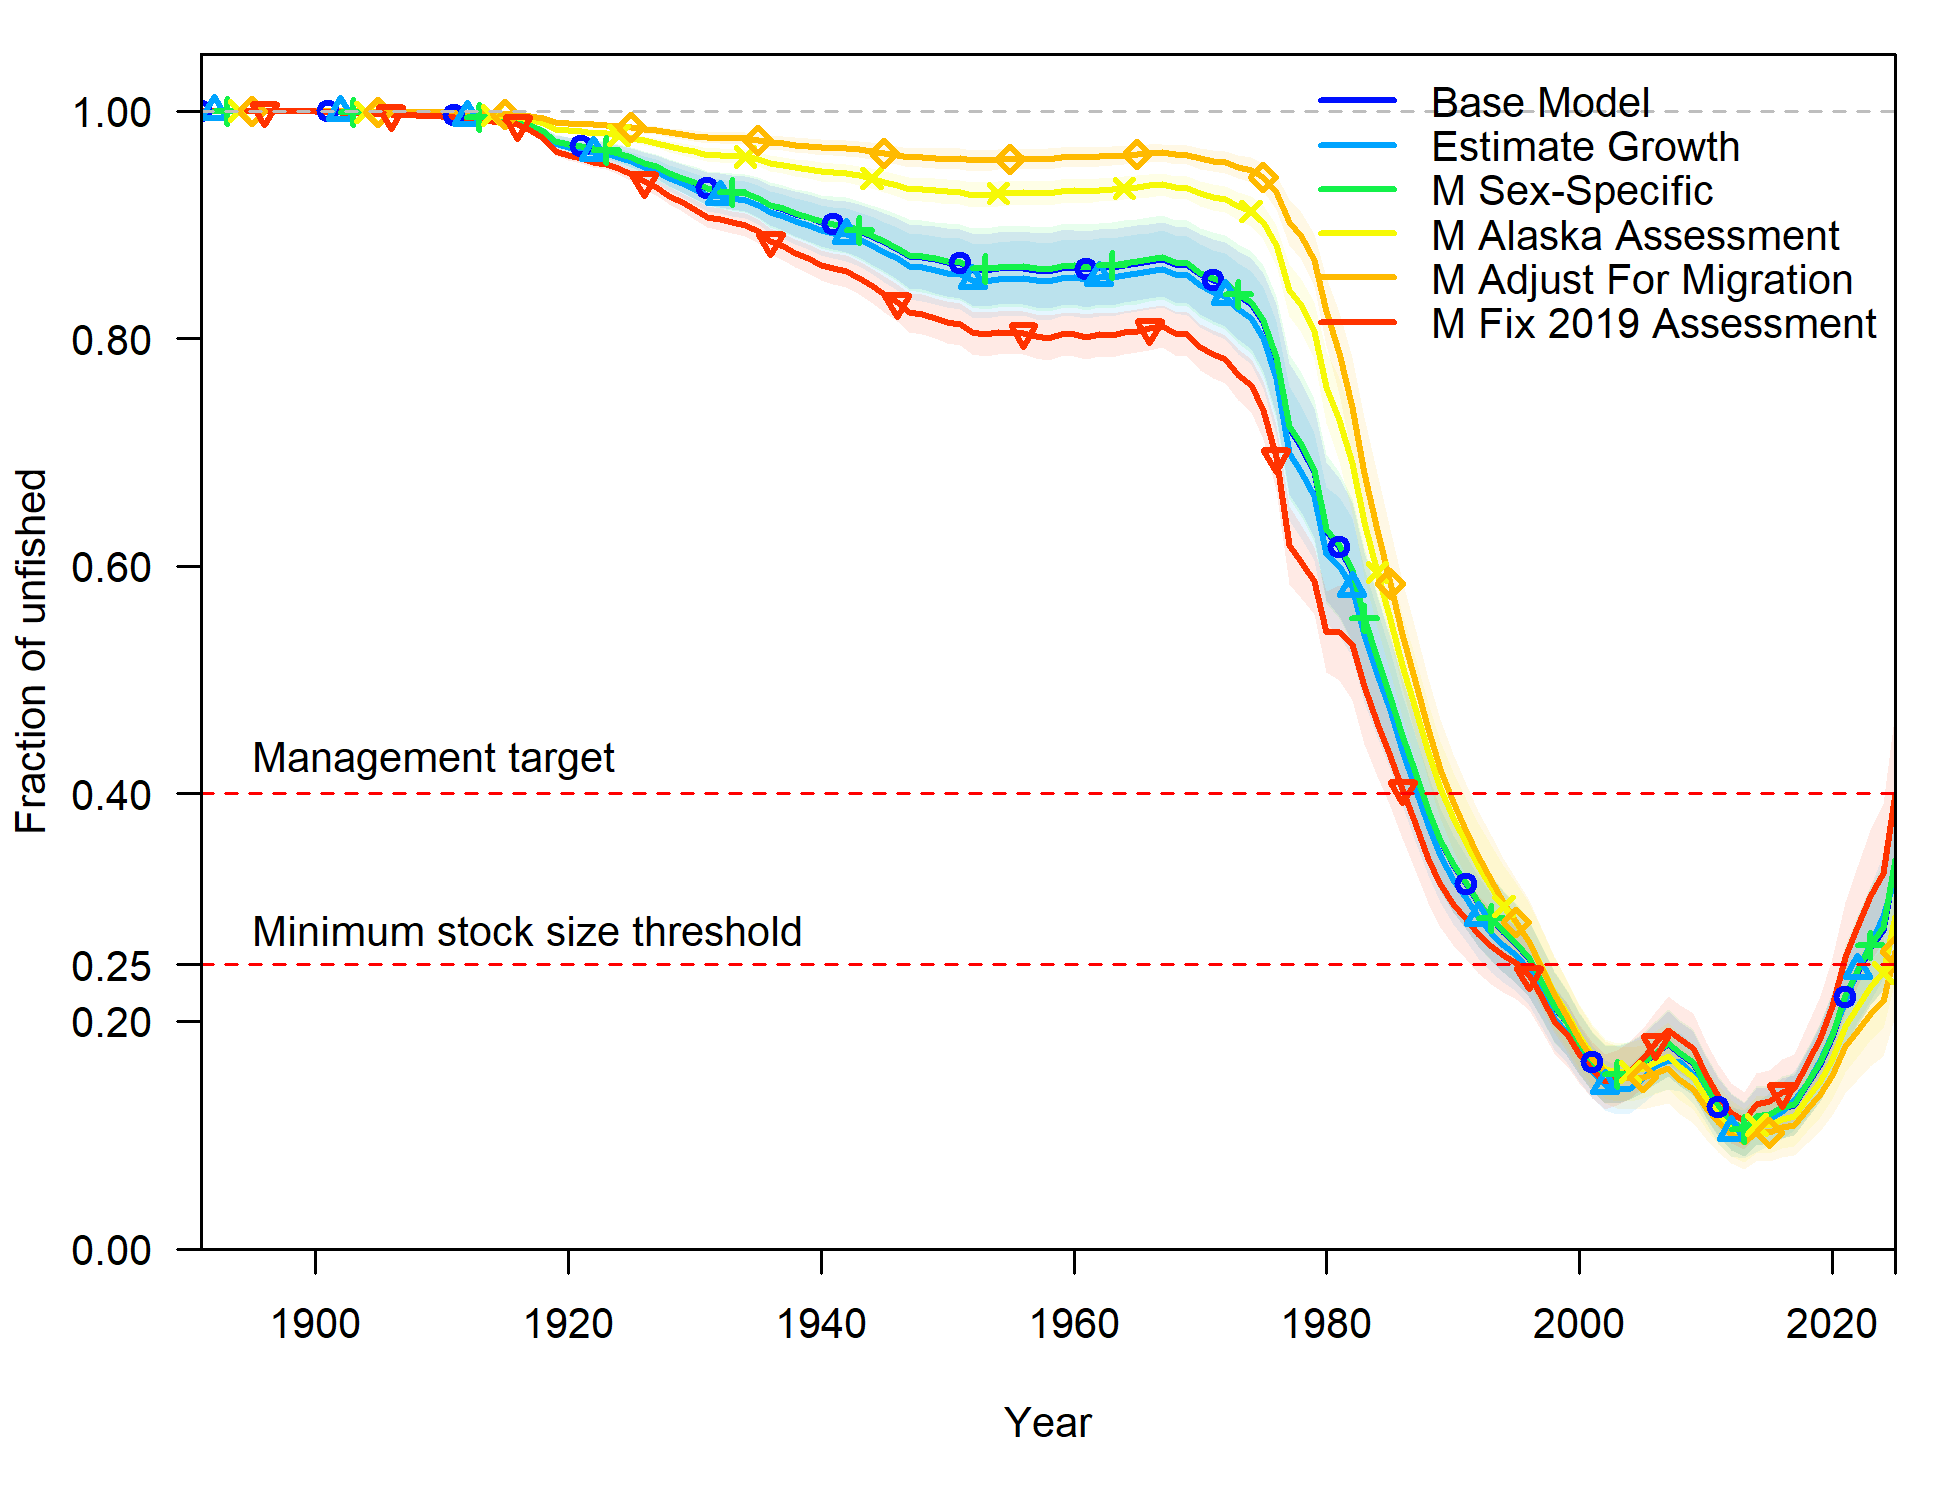
\includegraphics[width=1\linewidth,height=\textheight,keepaspectratio,alt={'Line plot with year on the x-axis and fraction of unfished on the y-axis.  In general, assuming the natural mortality values from the 2019 assessment, adjusting natural mortality for migration, or the natural mortality from the Alaska assessment results in trajectories that differ to the greatest extent from the base model. Select parameters and derived quanties are provided in Table 33.'}]{figures/sens_3_compare4_Bratio_uncertainty.png}

}

\caption{\label{fig-sens-3-bratio}Maximum likelihood estimates of
fraction of unfished (i.e., stock status) for the base model and
alternative sensitivity runs representing the estimation of growth
(rather than using an empircal weight-at-age approach for growth as in
the base model), the estimation of sex-specific natural mortality
(\emph{M}), and fixing \emph{M} at the value used in the assessment of
sablefish in Alaska, adjusted upwards to offset potential net emigration
to Canada, or set to sex-specific values used in the 2019 U.S. West
Coast assessment of sablefish. Shaded regions represent asymptotic 95
percent confidence intervals.}

\end{figure}%

\begin{figure}[H]

\centering{

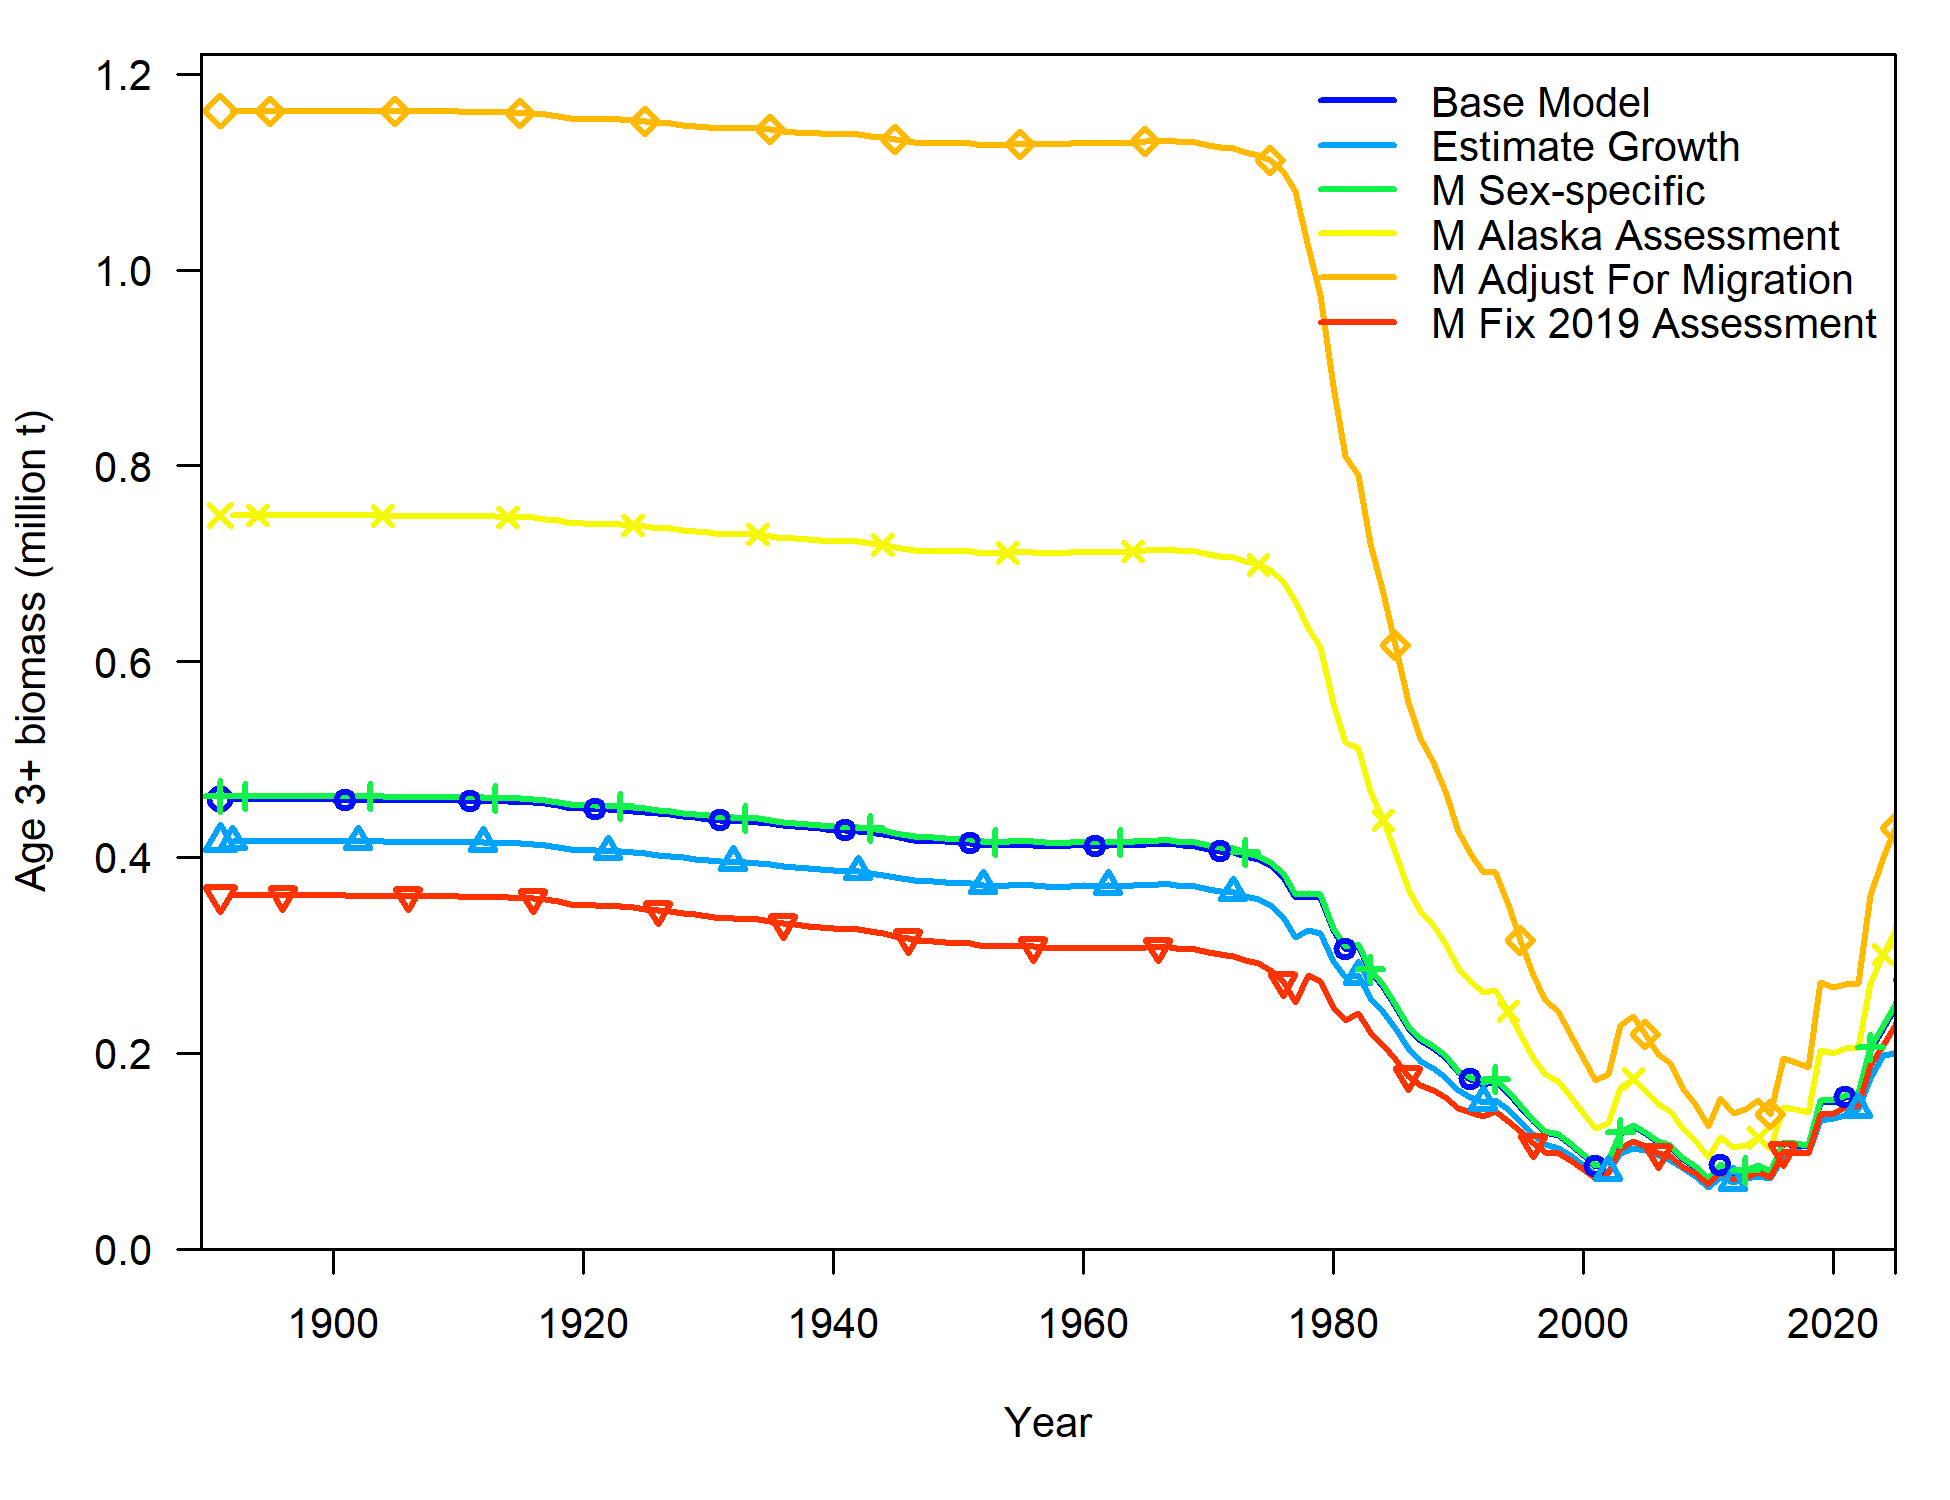
\includegraphics[width=1\linewidth,height=\textheight,keepaspectratio,alt={'Line plot with year on the x-axis and age 3 plus biomass on the y-axis.  In general, assuming the natural mortality values from the 2019 assessment, adjusting natural mortality for migration, or the natural mortality from the Alaska assessment results in trajectories that differ to the greatest extent from the base model. Select parameters and derived quanties are provided in Table 33.'}]{figures/sens_3_compare18_smrybio.png}

}

\caption{\label{fig-sens-3-sumB}Maximum likelihood estimates of summary
biomass (age 3 and older) for the base model and alternative sensitivity
runs representing the estimation of growth (rather than using an
empircal weight-at-age approach for growth as in the base model), the
estimation of sex-specific natural mortality (\emph{M}), and fixing
\emph{M} at the value used in the assessment of sablefish in Alaska,
adjusted upwards to offset potential net emigration to Canada, or set to
sex-specific values used in the 2019 U.S. West Coast assessment of
sablefish.}

\end{figure}%

\begin{figure}[H]

\centering{

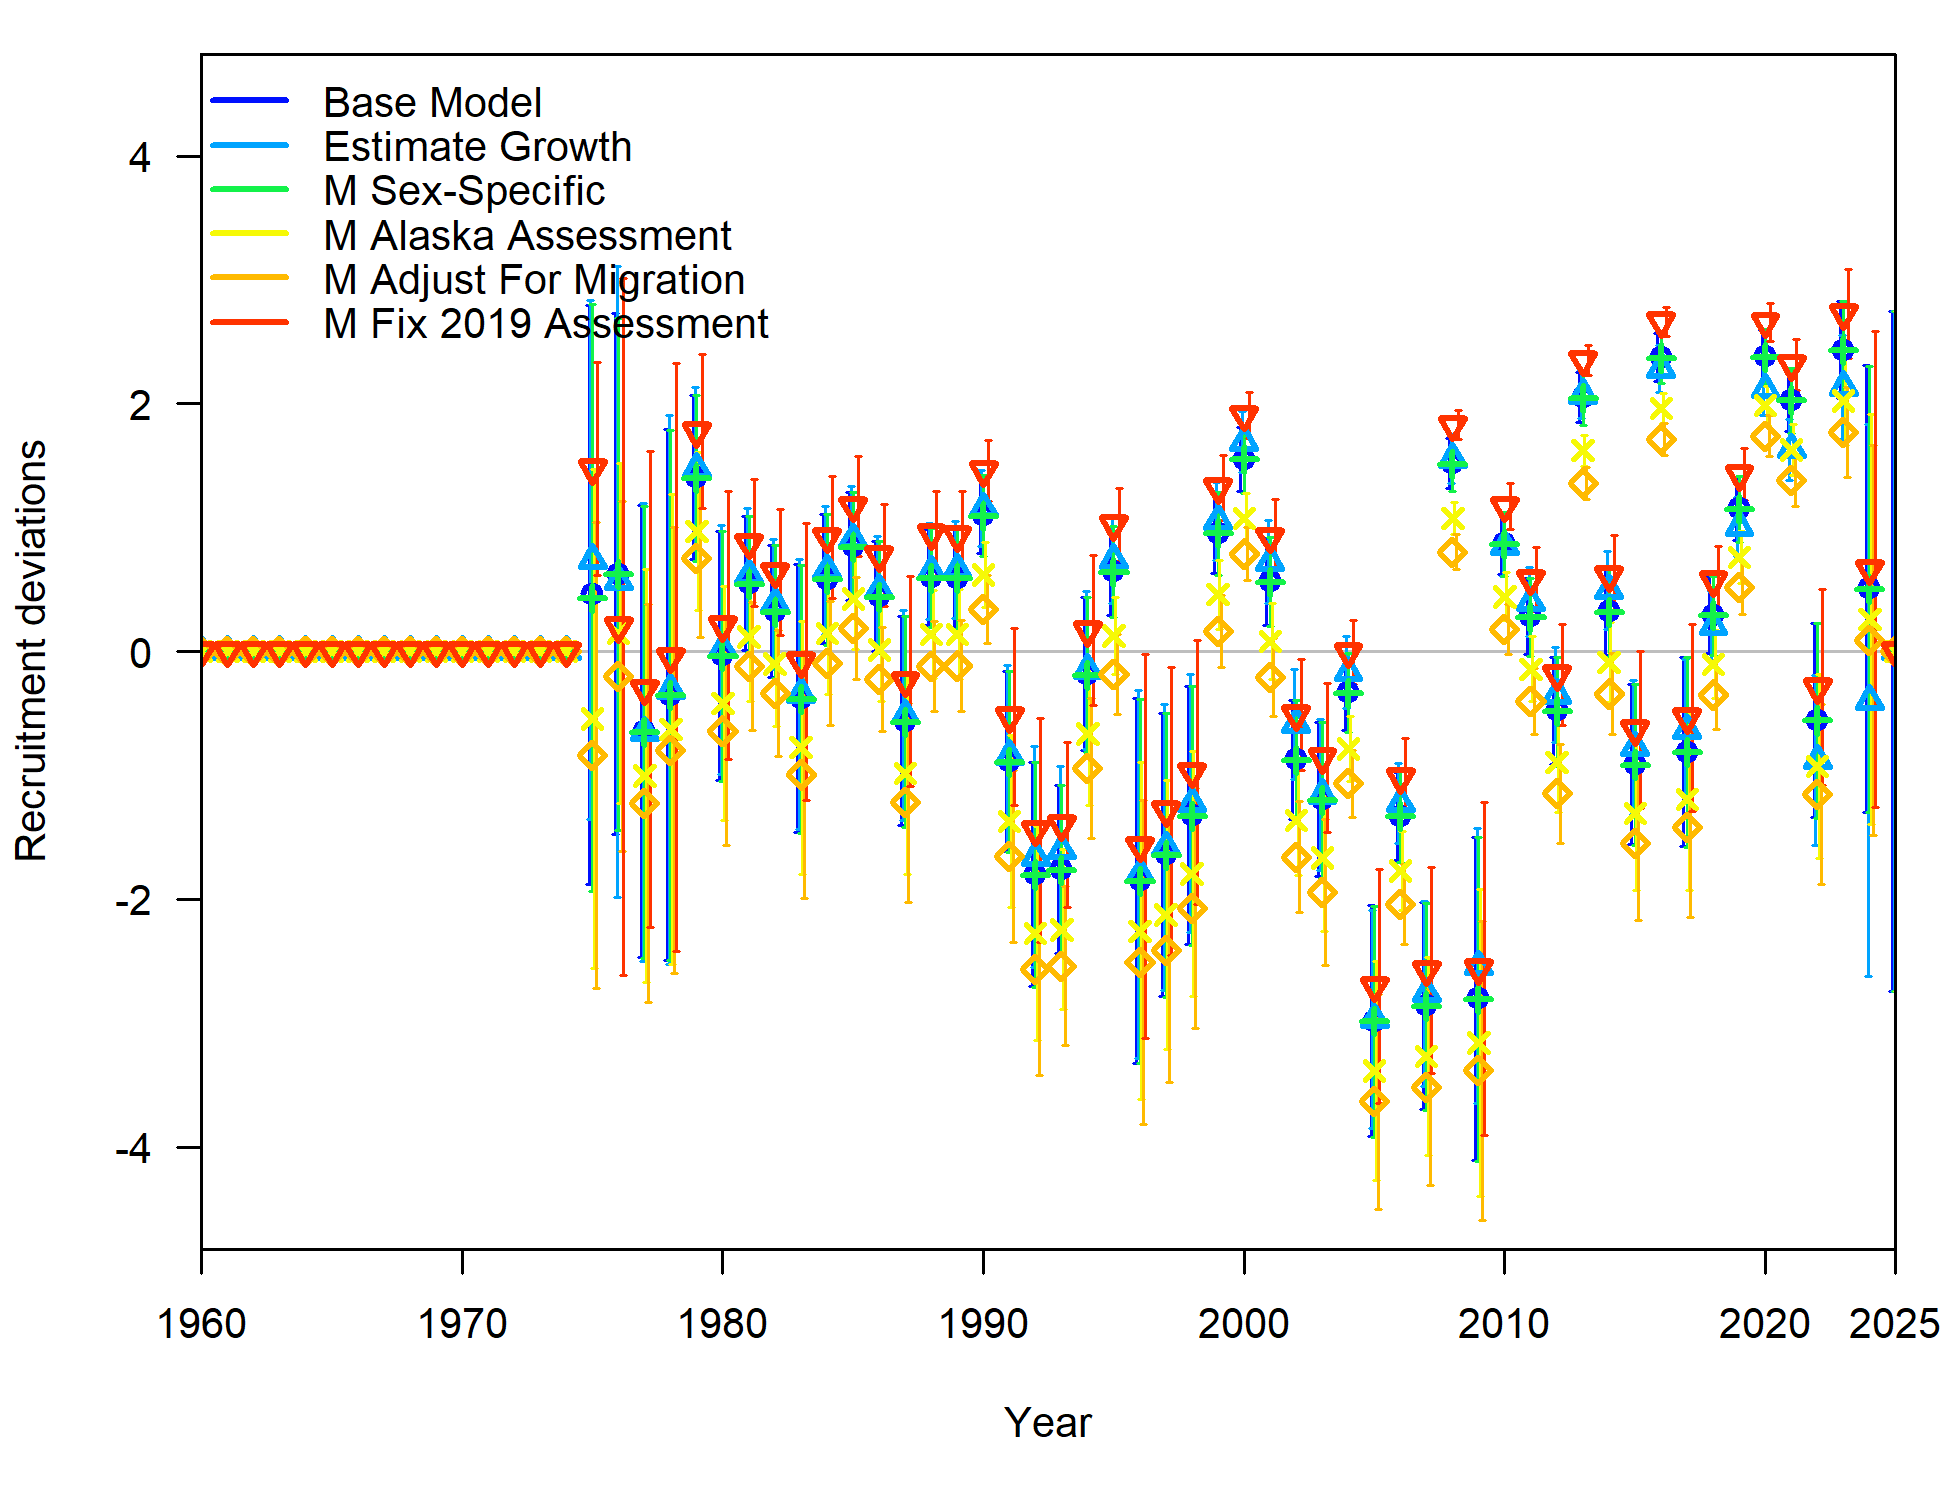
\includegraphics[width=1\linewidth,height=\textheight,keepaspectratio,alt={'Line plot with year on the x-axis and annual recruitment deviations in log-space on the y-axis. For each sensitivity that assumes an alternative value for natural mortality the annual recruitment deviations differ to the greatest extent from the base model. Select parameters and derived quanties are provided in Table 33.'}]{figures/sens_3_compare12_recdevs_uncertainty.png}

}

\caption{\label{fig-sens-3-recdev}Maximum likelihood estimates of
recruitment deviations from 1960-2025 for the base model and alternative
sensitivity runs representing the estimation of growth (rather than
using an empircal weight-at-age approach for growth as in the base
model), the estimation of sex-specific natural mortality (\emph{M}), and
fixing \emph{M} at the value used in the assessment of sablefish in
Alaska, adjusted upwards to offset potential net emigration to Canada,
or set to sex-specific values used in the 2019 U.S. West Coast
assessment of sablefish. Bars represent asymptotic 95 percent confidence
intervals.}

\end{figure}%

\begin{figure}[H]

\centering{

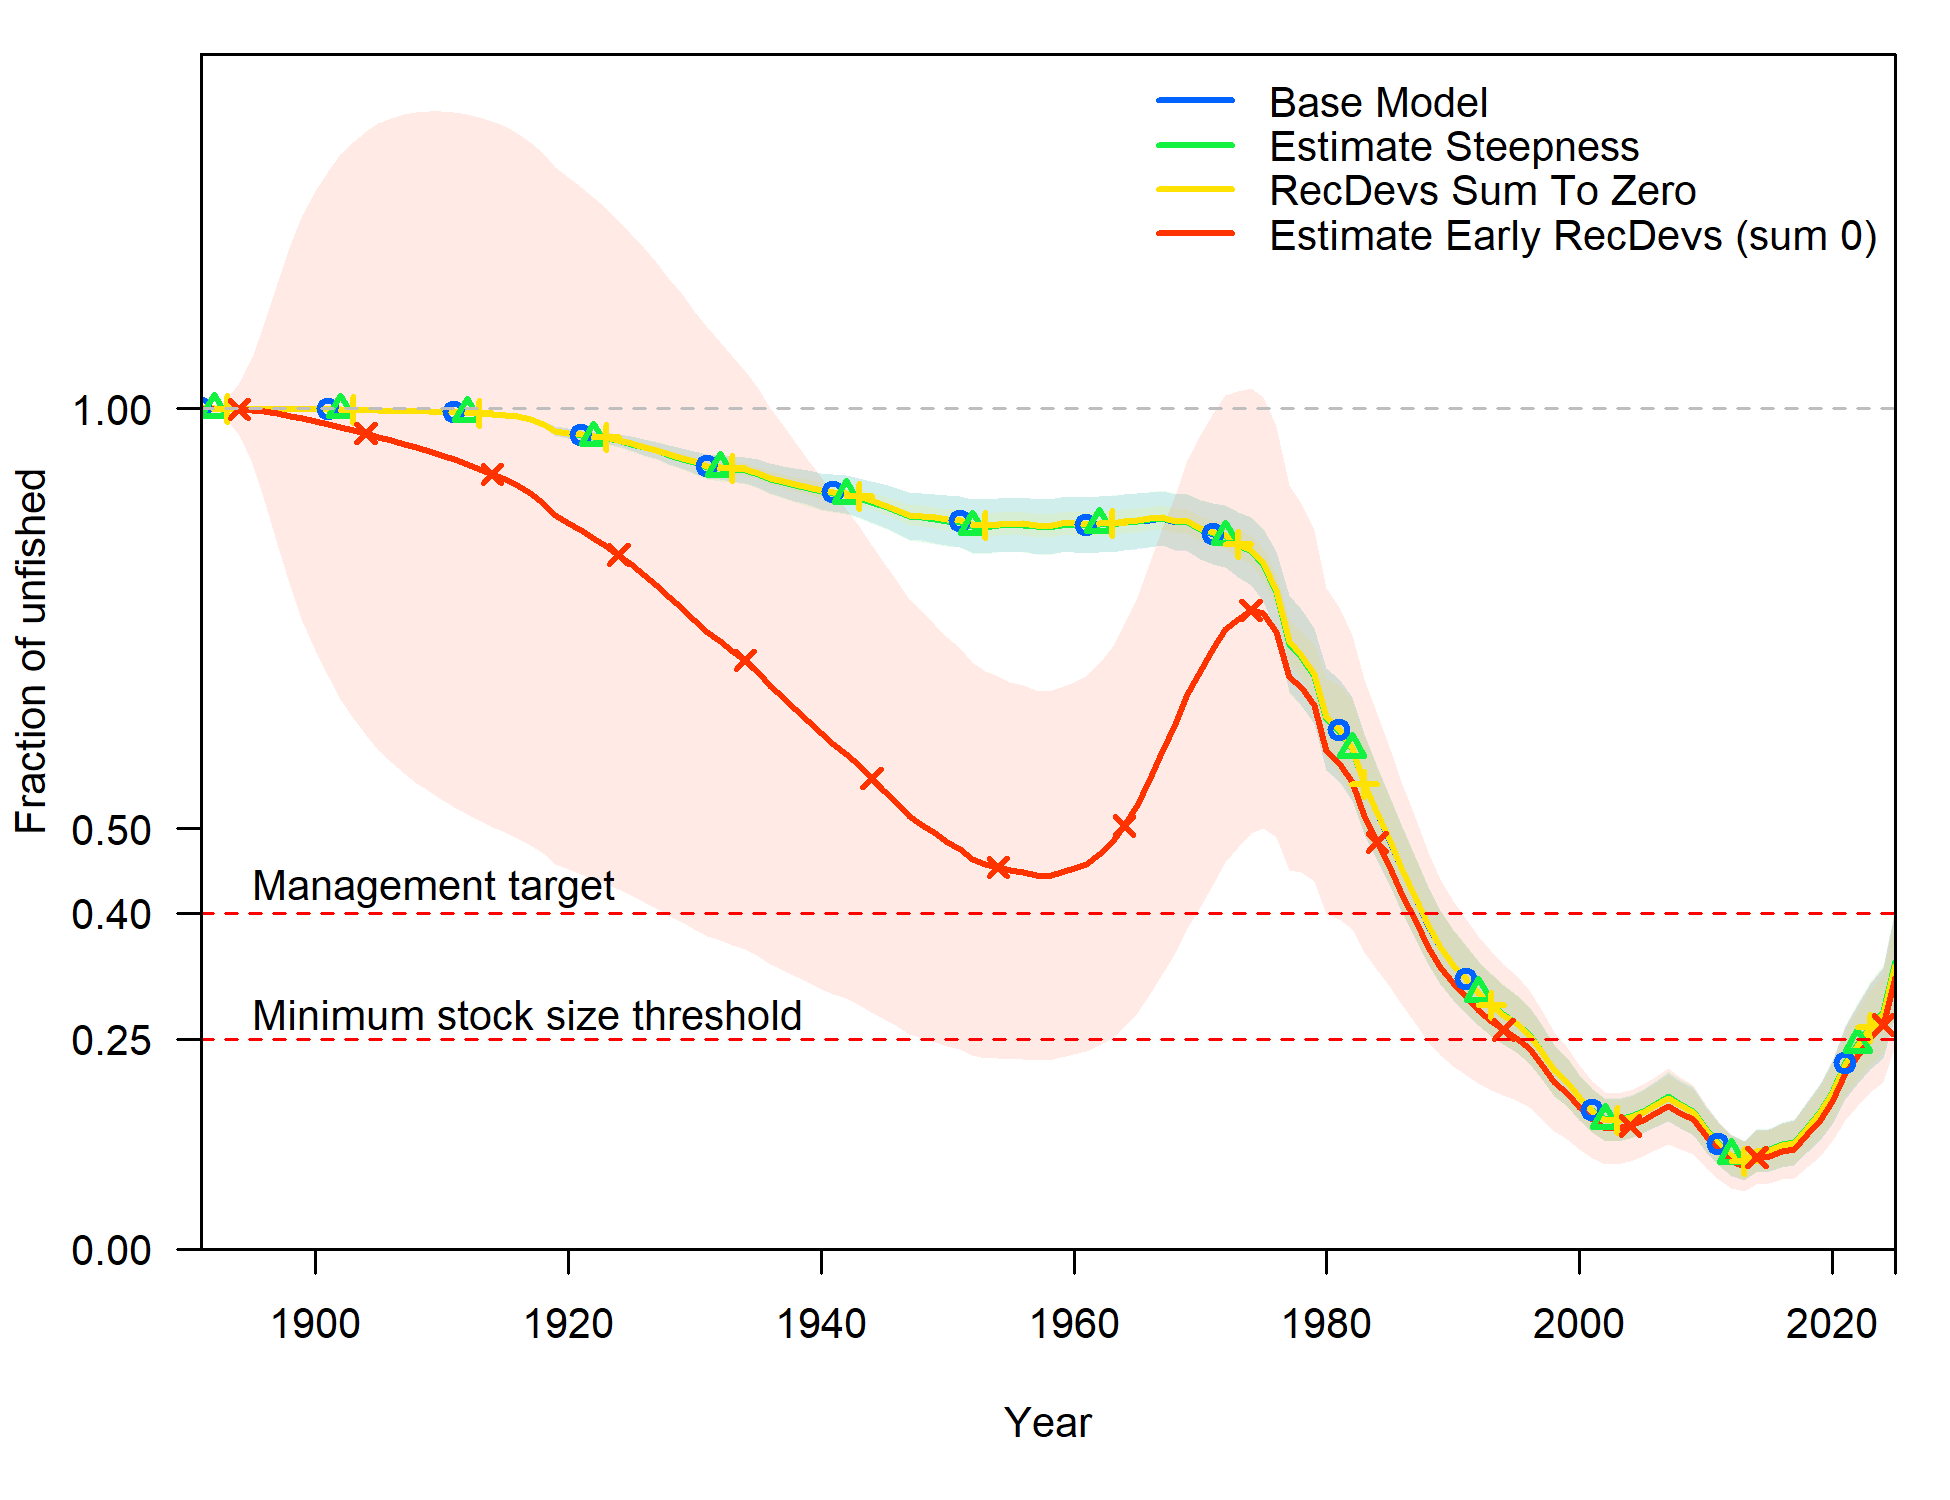
\includegraphics[width=1\linewidth,height=\textheight,keepaspectratio,alt={'Line plot with year on the x-axis and fraction of unfished on the y-axis. The sensitivity that estimates early recruitment deviations results in a trajectory the declines sharply from 1890 to 1960 to 0.43, increases from 1961 to 1980 to 0.80, and then declines and is similar to the base model from 1980 to 2025. The sensitivity that forces annual recruitment deviations to sum to zero has nearly an identical trajectory to the base model. Select parameters and derived quanties are provided in Table 34.'}]{figures/sens_4_compare4_Bratio_uncertainty.png}

}

\caption{\label{fig-sens-4-bratio}Maximum likelihood estimates of
fraction of unfished (i.e., stock status) for the base model and
alternative sensitivity runs representing the estimaton of steepness
(\emph{h}), imposing the restriction that recruitment deviations in the
main recruitment period must sum to zero, and estimating early
(1890-1974) recruitment deviations with the sum to zero constraint
imposed. Shaded regions represent asymptotic 95 percent confidence
intervals.}

\end{figure}%

\begin{figure}[H]

\centering{

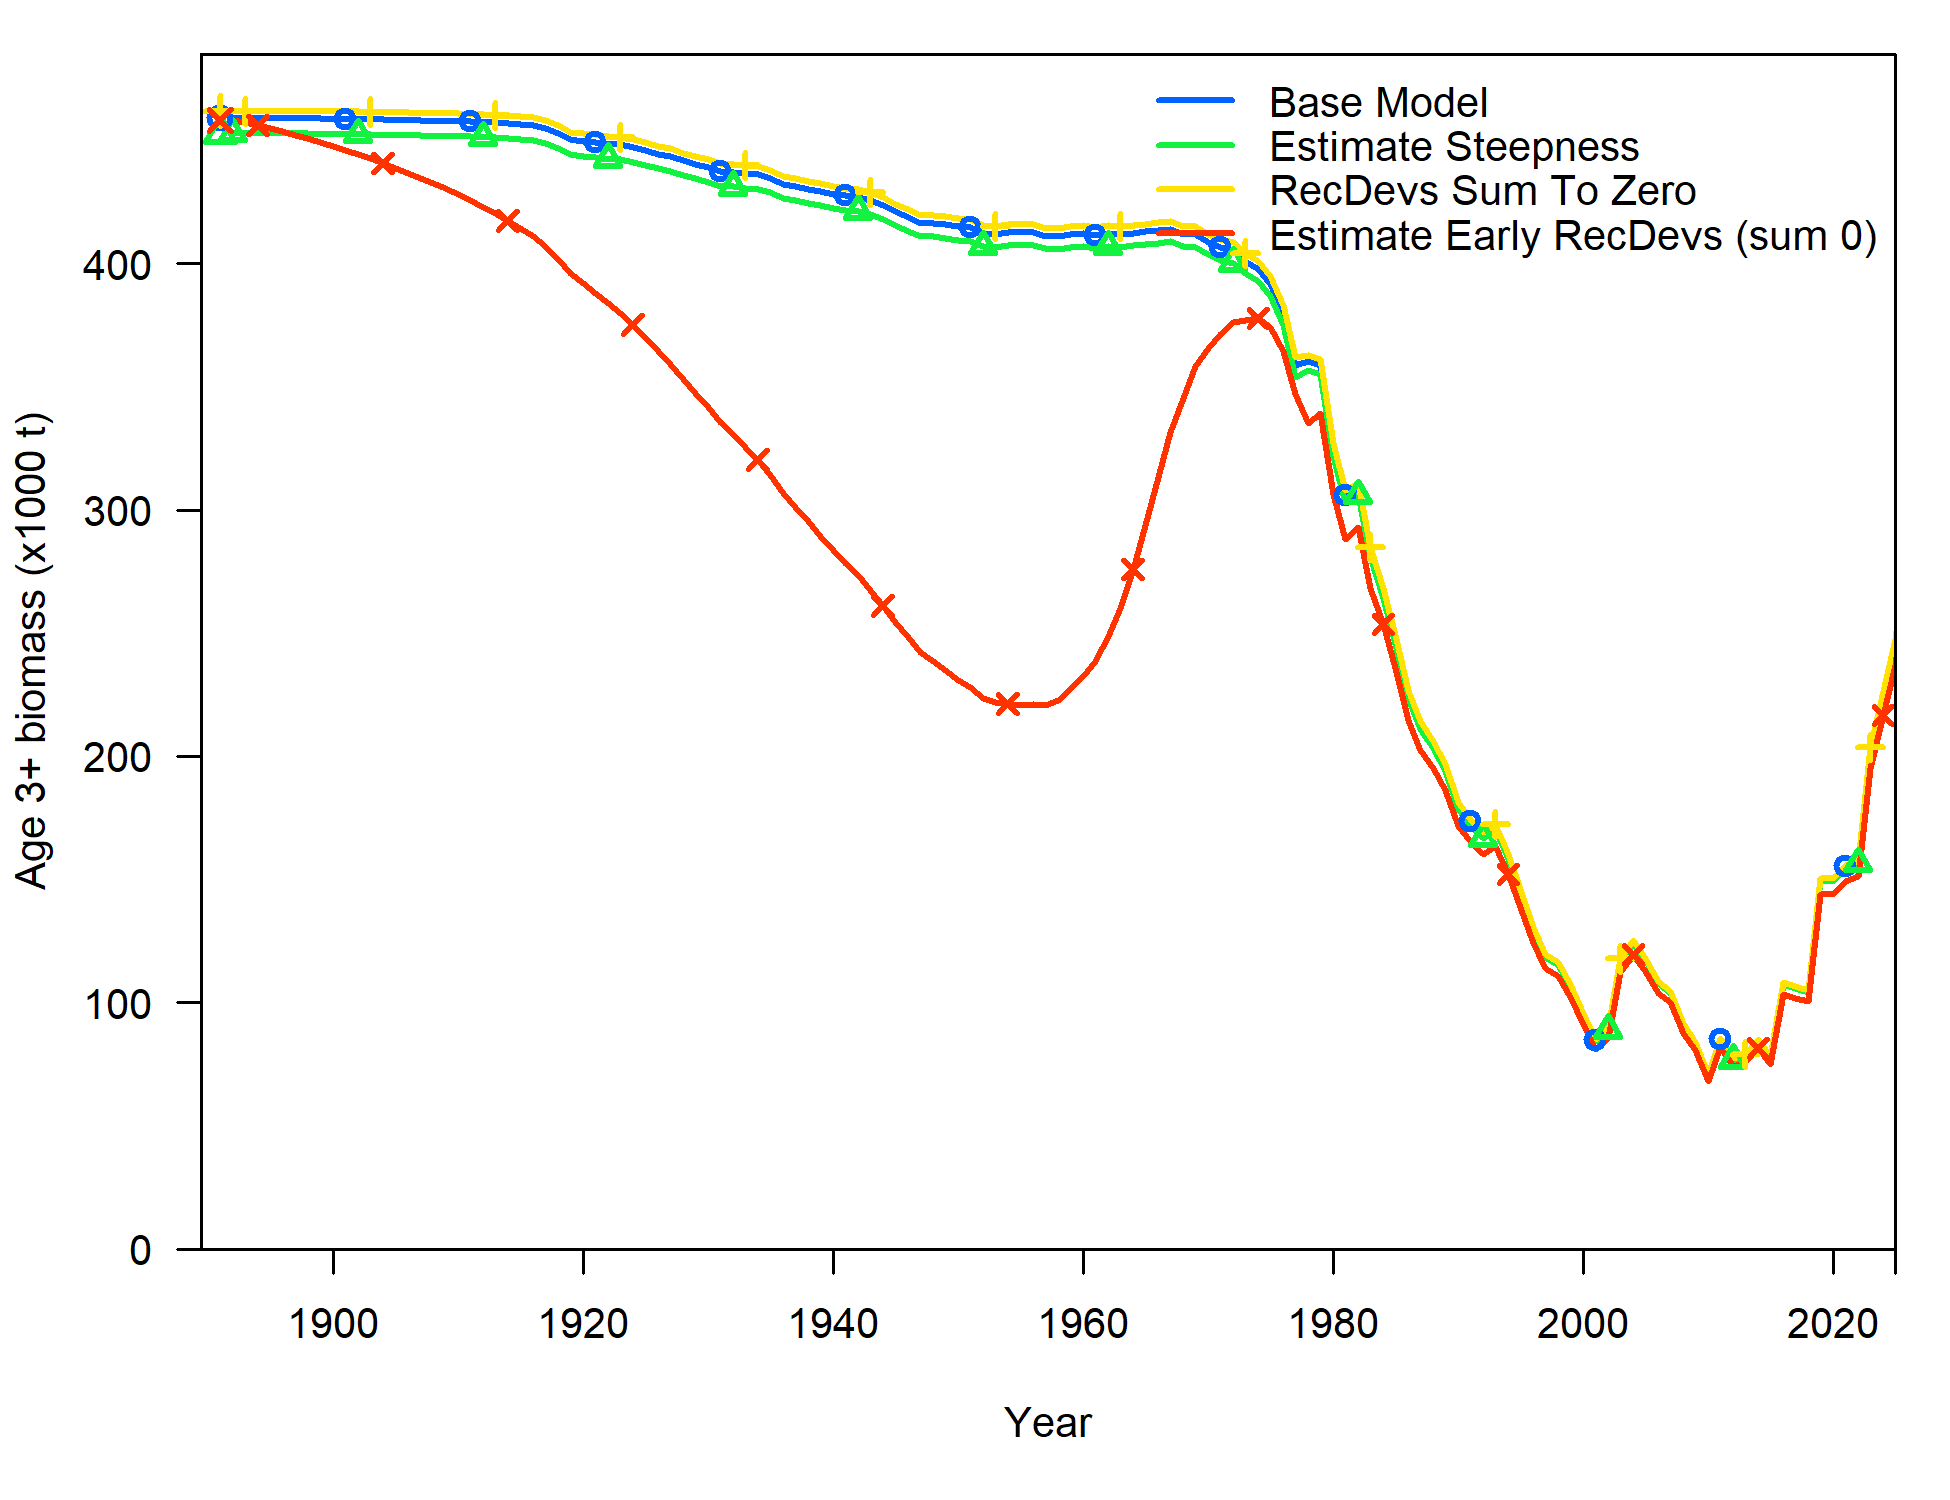
\includegraphics[width=1\linewidth,height=\textheight,keepaspectratio,alt={'Line plot with year on the x-axis and age 3 plus biomass on the y-axis. The sensitivity that estimates early recruitment deviations results in a trajectory the declines sharply from 1890 to 1960, increases from 1961 to 1980, and then declines and is similar to the base model from 1980 to 2025. The sensitivity that forces annual recruitment deviations to sum to zero has nearly an identical trajectory to the base model. Select parameters and derived quanties are provided in Table 34.'}]{figures/sens_4_compare18_smrybio.png}

}

\caption{\label{fig-sens-4-sumB}Maximum likelihood estimates of summary
biomass (age 3 and older) for the base model and alternative sensitivity
runs representing the estimaton of steepness (\emph{h}), imposing the
restriction that recruitment deviations in the main recruitment period
must sum to zero, and estimating early (1890-1974) recruitment
deviations with the sum to zero constraint imposed.}

\end{figure}%

\begin{figure}[H]

\centering{

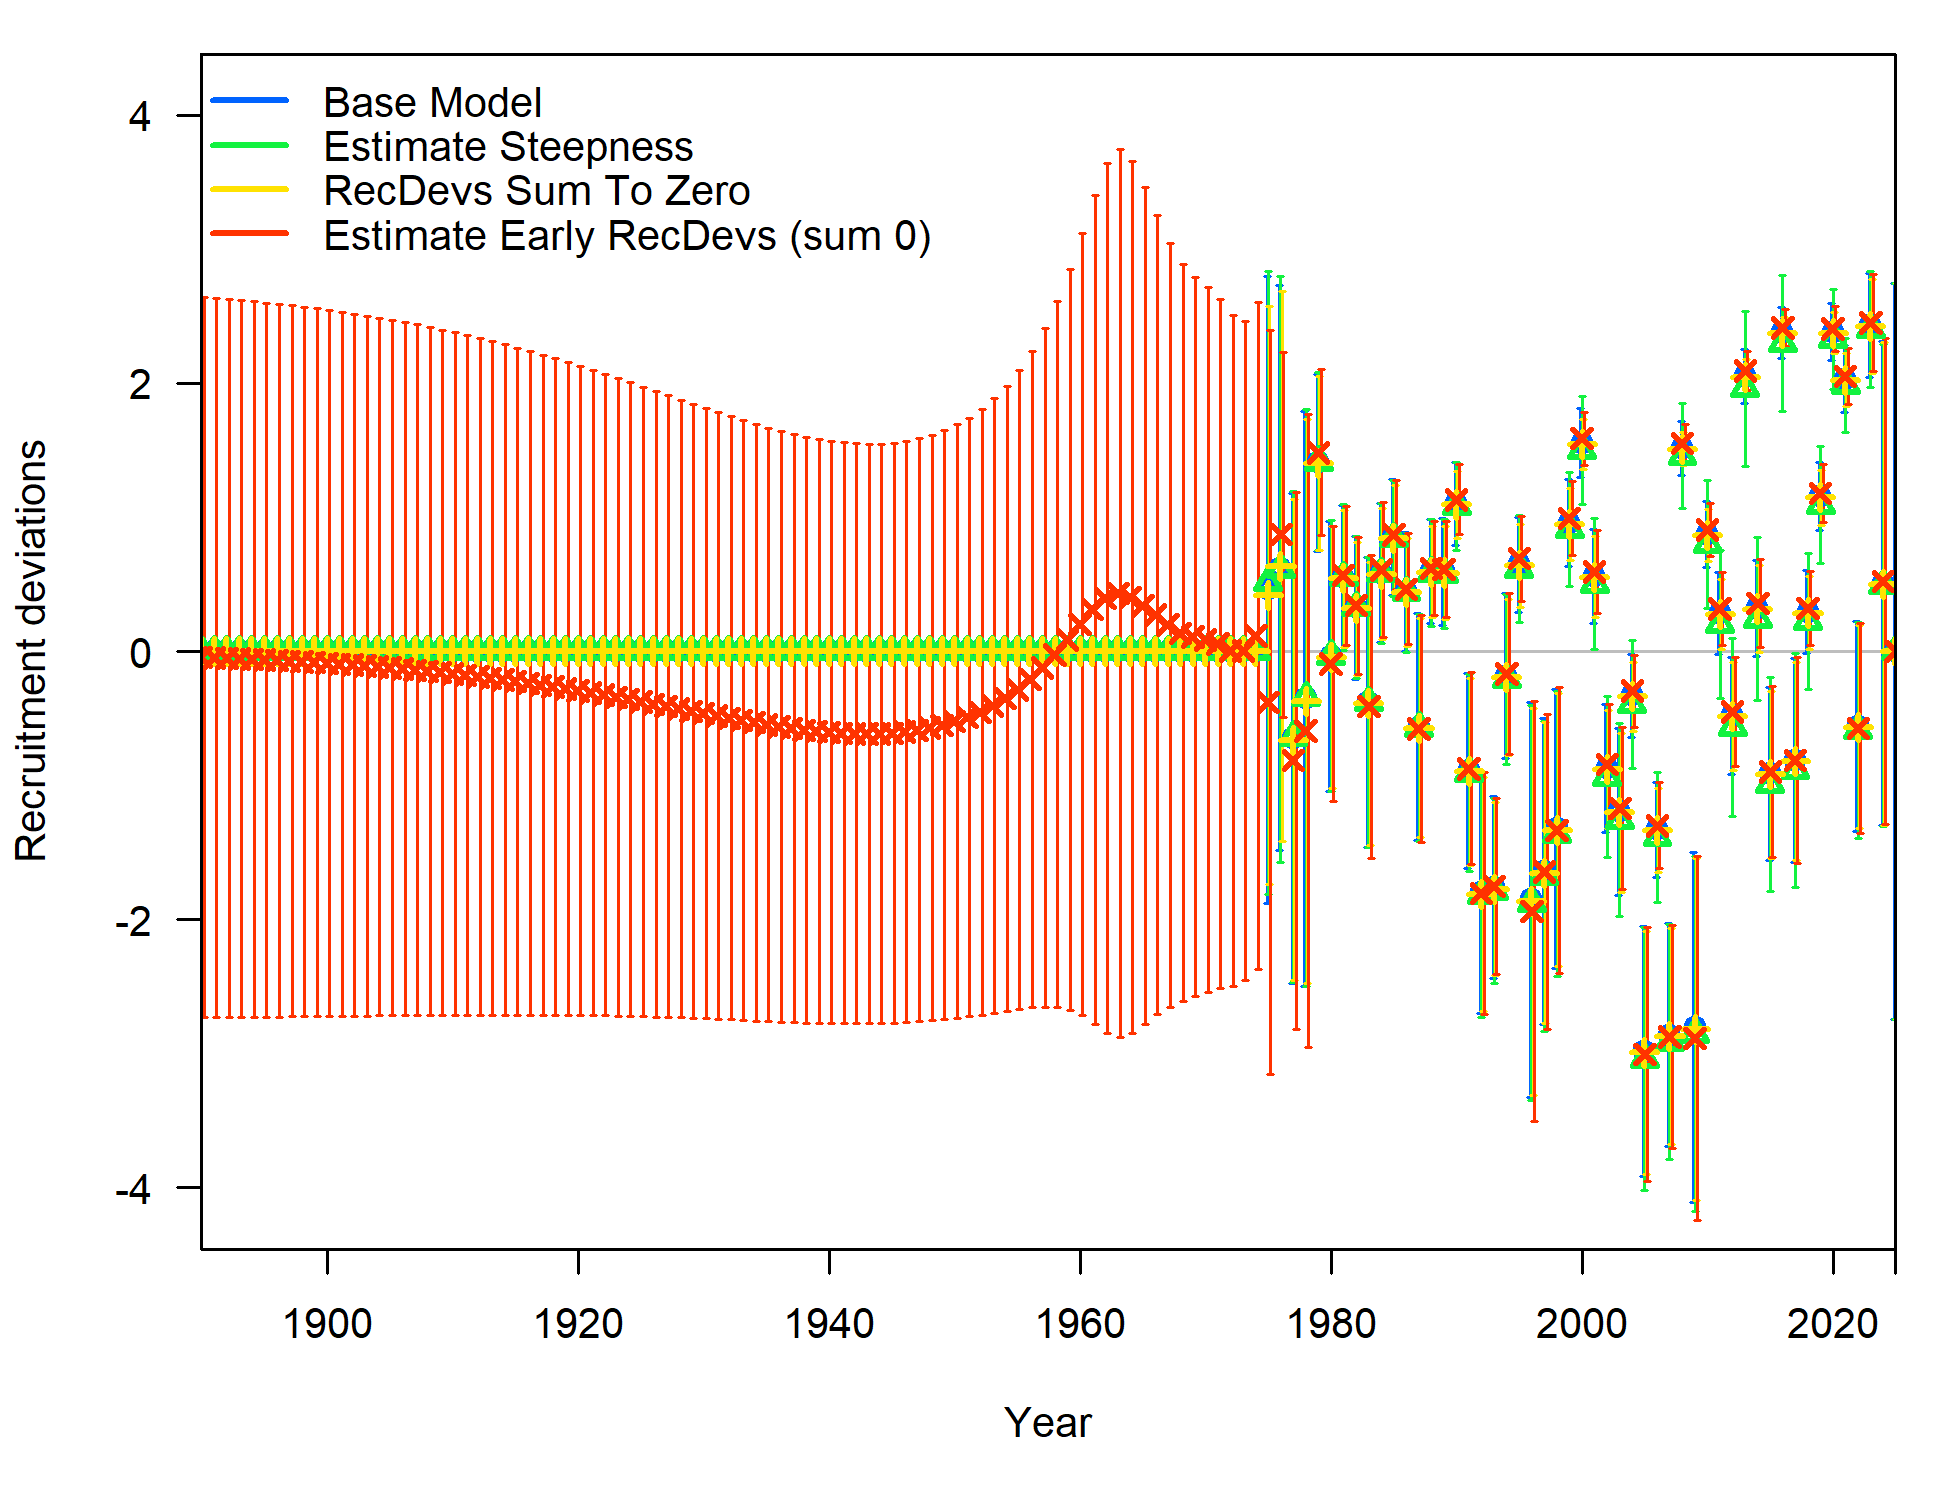
\includegraphics[width=1\linewidth,height=\textheight,keepaspectratio,alt={'Line plot with year on the x-axis and annual recruitment deviations in log-space on the y-axis. The sensitivity that estimates early recruitment deviations estimates negative deviations from 1980 to 1957, positive deviations from 1958 to 1975, and then similar deviations to the base model from 1976 to 2024. The sensitivity that forces annual recruitment deviations to sum to zero estimates nearly identical recruitment deviations to the base model. Select parameters and derived quanties are provided in Table 34.'}]{figures/sens_4_compare12_recdevs_uncertainty.png}

}

\caption{\label{fig-sens-4-recdev}Maximum likelihood estimates of
recruitment deviations for the base model and alternative sensitivity
runs representing the estimaton of steepness (\emph{h}), imposing the
restriction that recruitment deviations in the main recruitment period
must sum to zero, and estimating early (1890-1974) recruitment
deviations with the sum to zero constraint imposed. Bars represent
asymptotic 95 percent confidence intervals.}

\end{figure}%

\begin{figure}[H]

\centering{

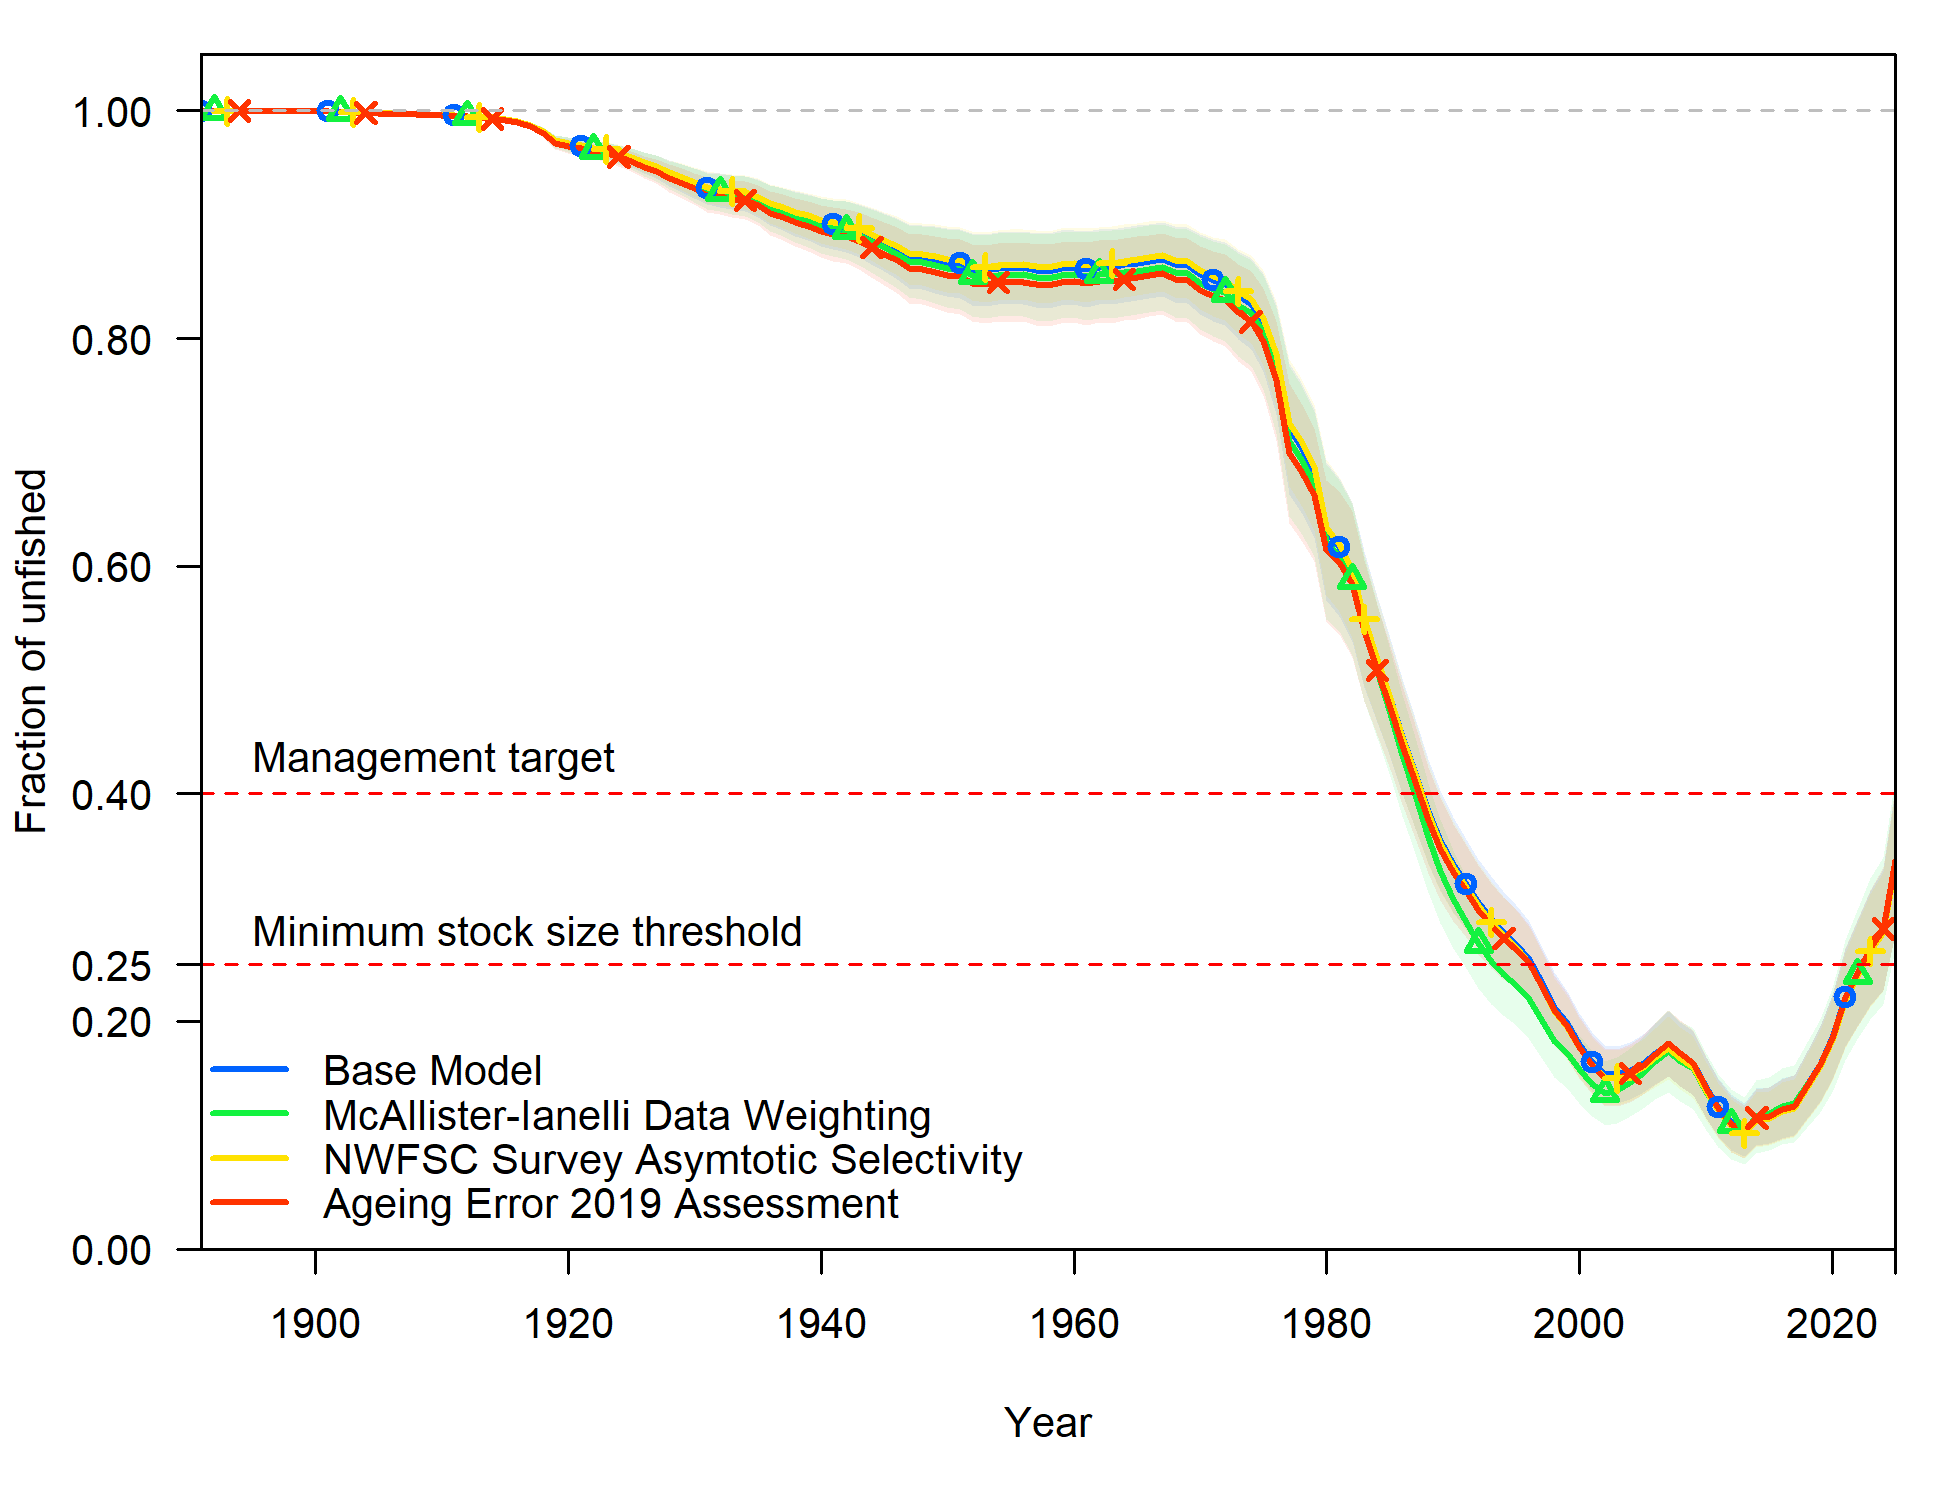
\includegraphics[width=1\linewidth,height=\textheight,keepaspectratio,alt={'Line plot with year on the x-axis and fraction of unfished on the y-axis. Each of the sensitivities has nearly identical trajectories compared to the base model. Select parameters and derived quanties are provided in Table 35.'}]{figures/sens_2_compare4_Bratio_uncertainty.png}

}

\caption{\label{fig-sens-2-bratio}Maximum likelihood estimates of
fraction of unfished (i.e., stock status) for the base model and
alternative sensitivity runs representing the use of the
McAllister-Ianelli harmonic mean method for weighting composition data,
the specification of asymptotic selectivity for NWFSC Surveys, and using
the ageing error vector applied in the 2019 stock assessment. Shaded
regions represent asymptotic 95 percent confidence intervals.}

\end{figure}%

\begin{figure}[H]

\centering{

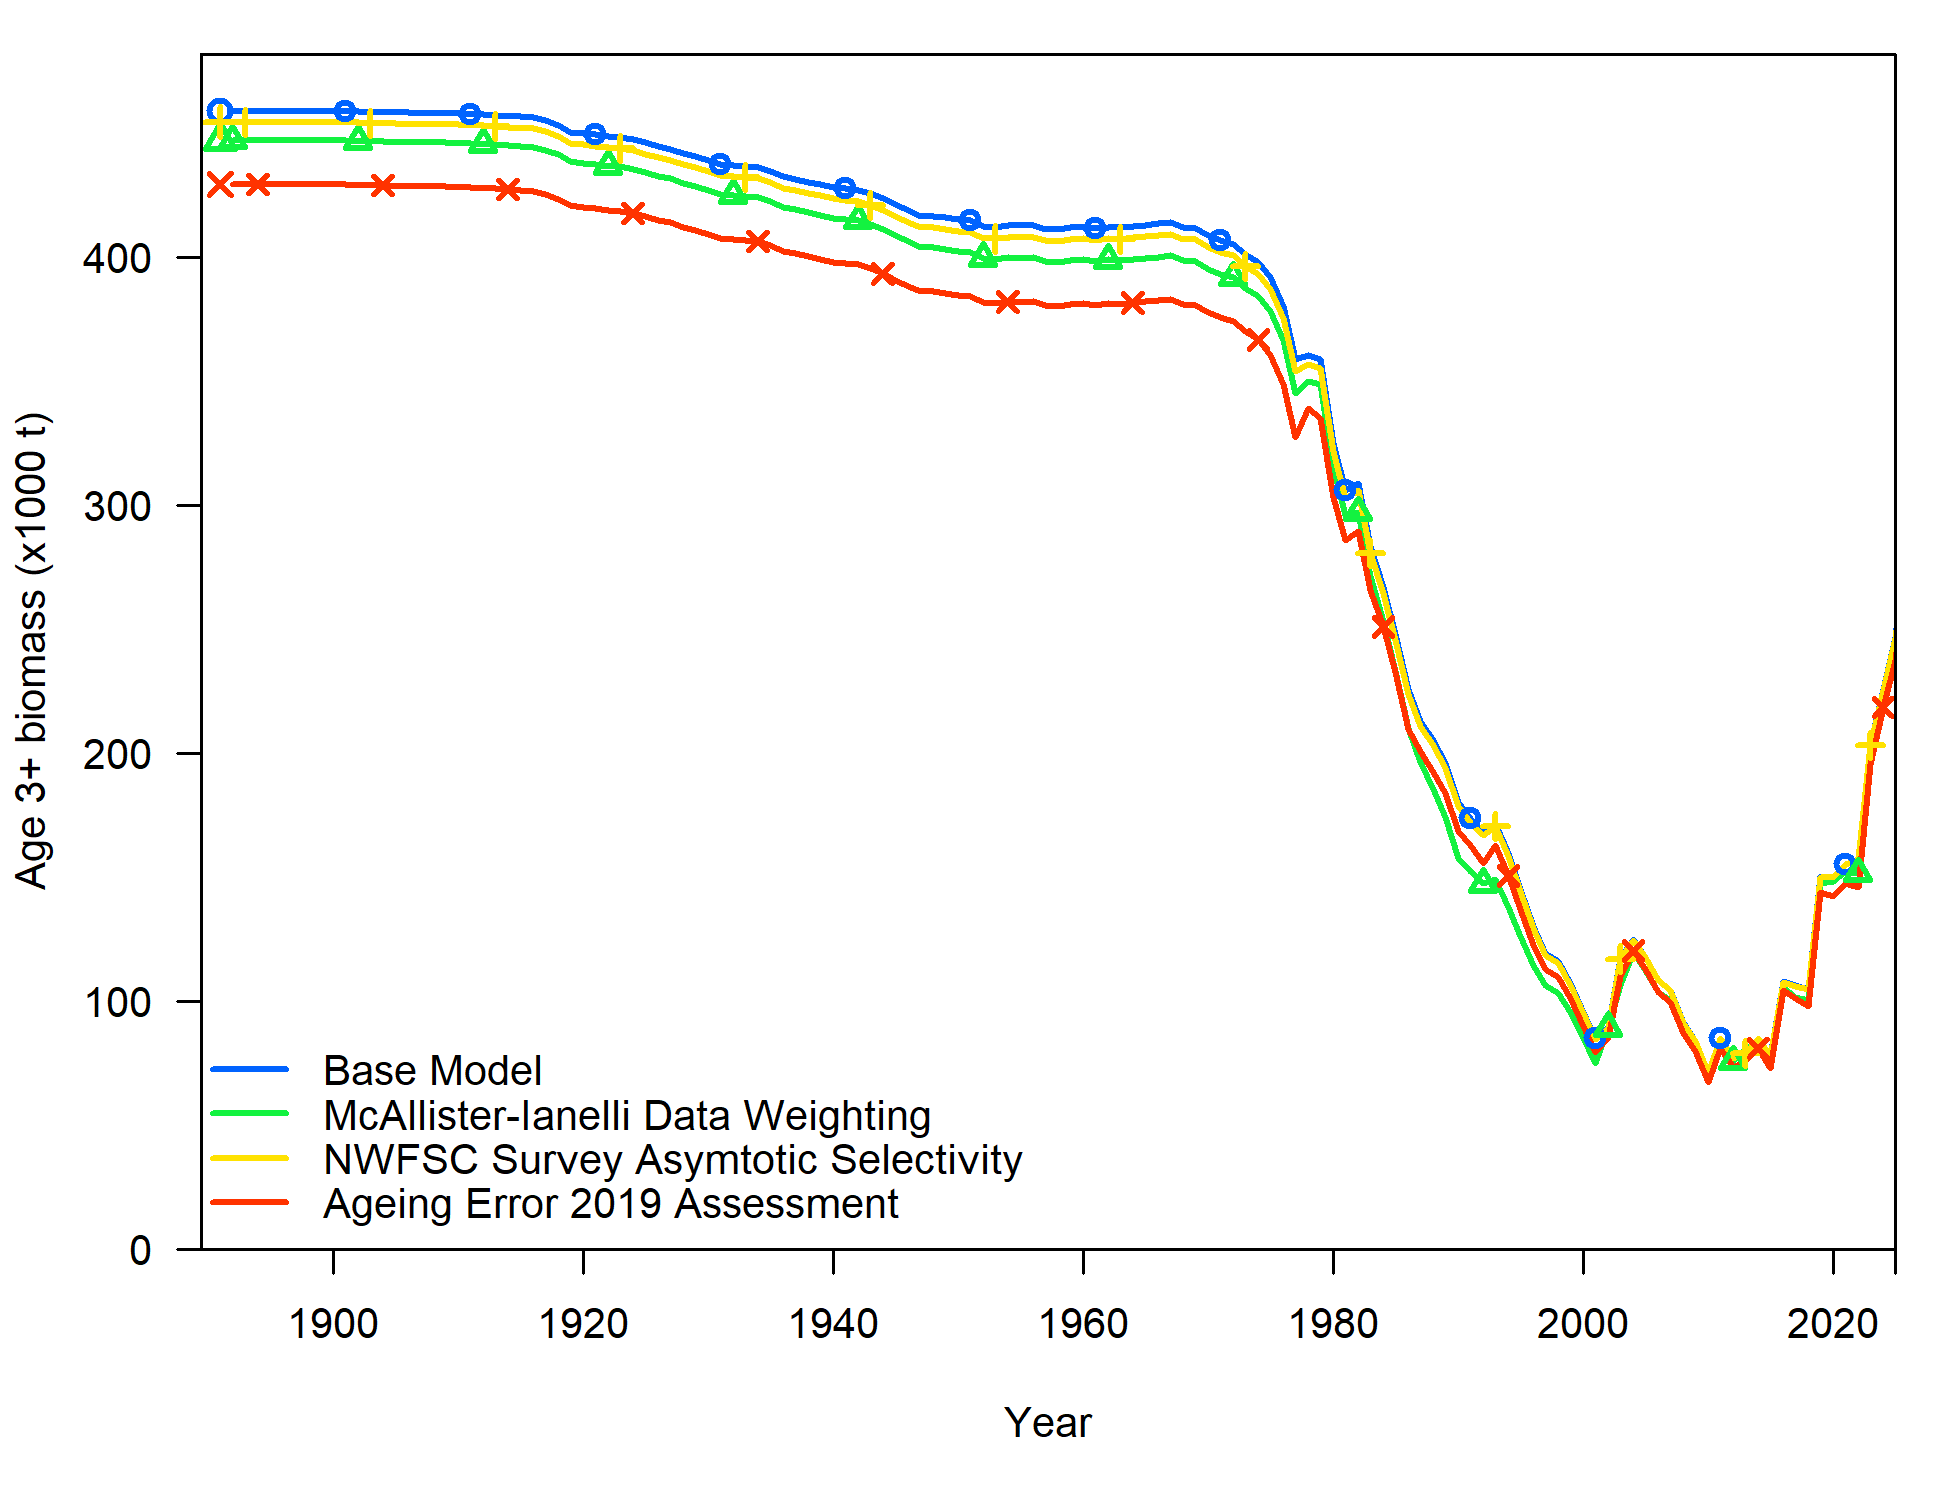
\includegraphics[width=1\linewidth,height=\textheight,keepaspectratio,alt={'Line plot with year on the x-axis and age 3 plus biomass on the y-axis. Each of the sensitivities has nearly identical trajectories compared to the base model from 1890 to 2025 with minor differences in the unfished age 3 plus biomass estimates. Select parameters and derived quanties are provided in Table 35.'}]{figures/sens_2_compare18_smrybio.png}

}

\caption{\label{fig-sens-2-sumB}Maximum likelihood estimates of summary
biomass (age 3 and older) for the base model and alternative sensitivity
runs representing the use of the McAllister-Ianelli harmonic mean method
for weighting composition data, the specification of asymptotic
selectivity for NWFSC Surveys, and using the ageing error vector applied
in the 2019 stock assessment.}

\end{figure}%

\begin{figure}[H]

\centering{

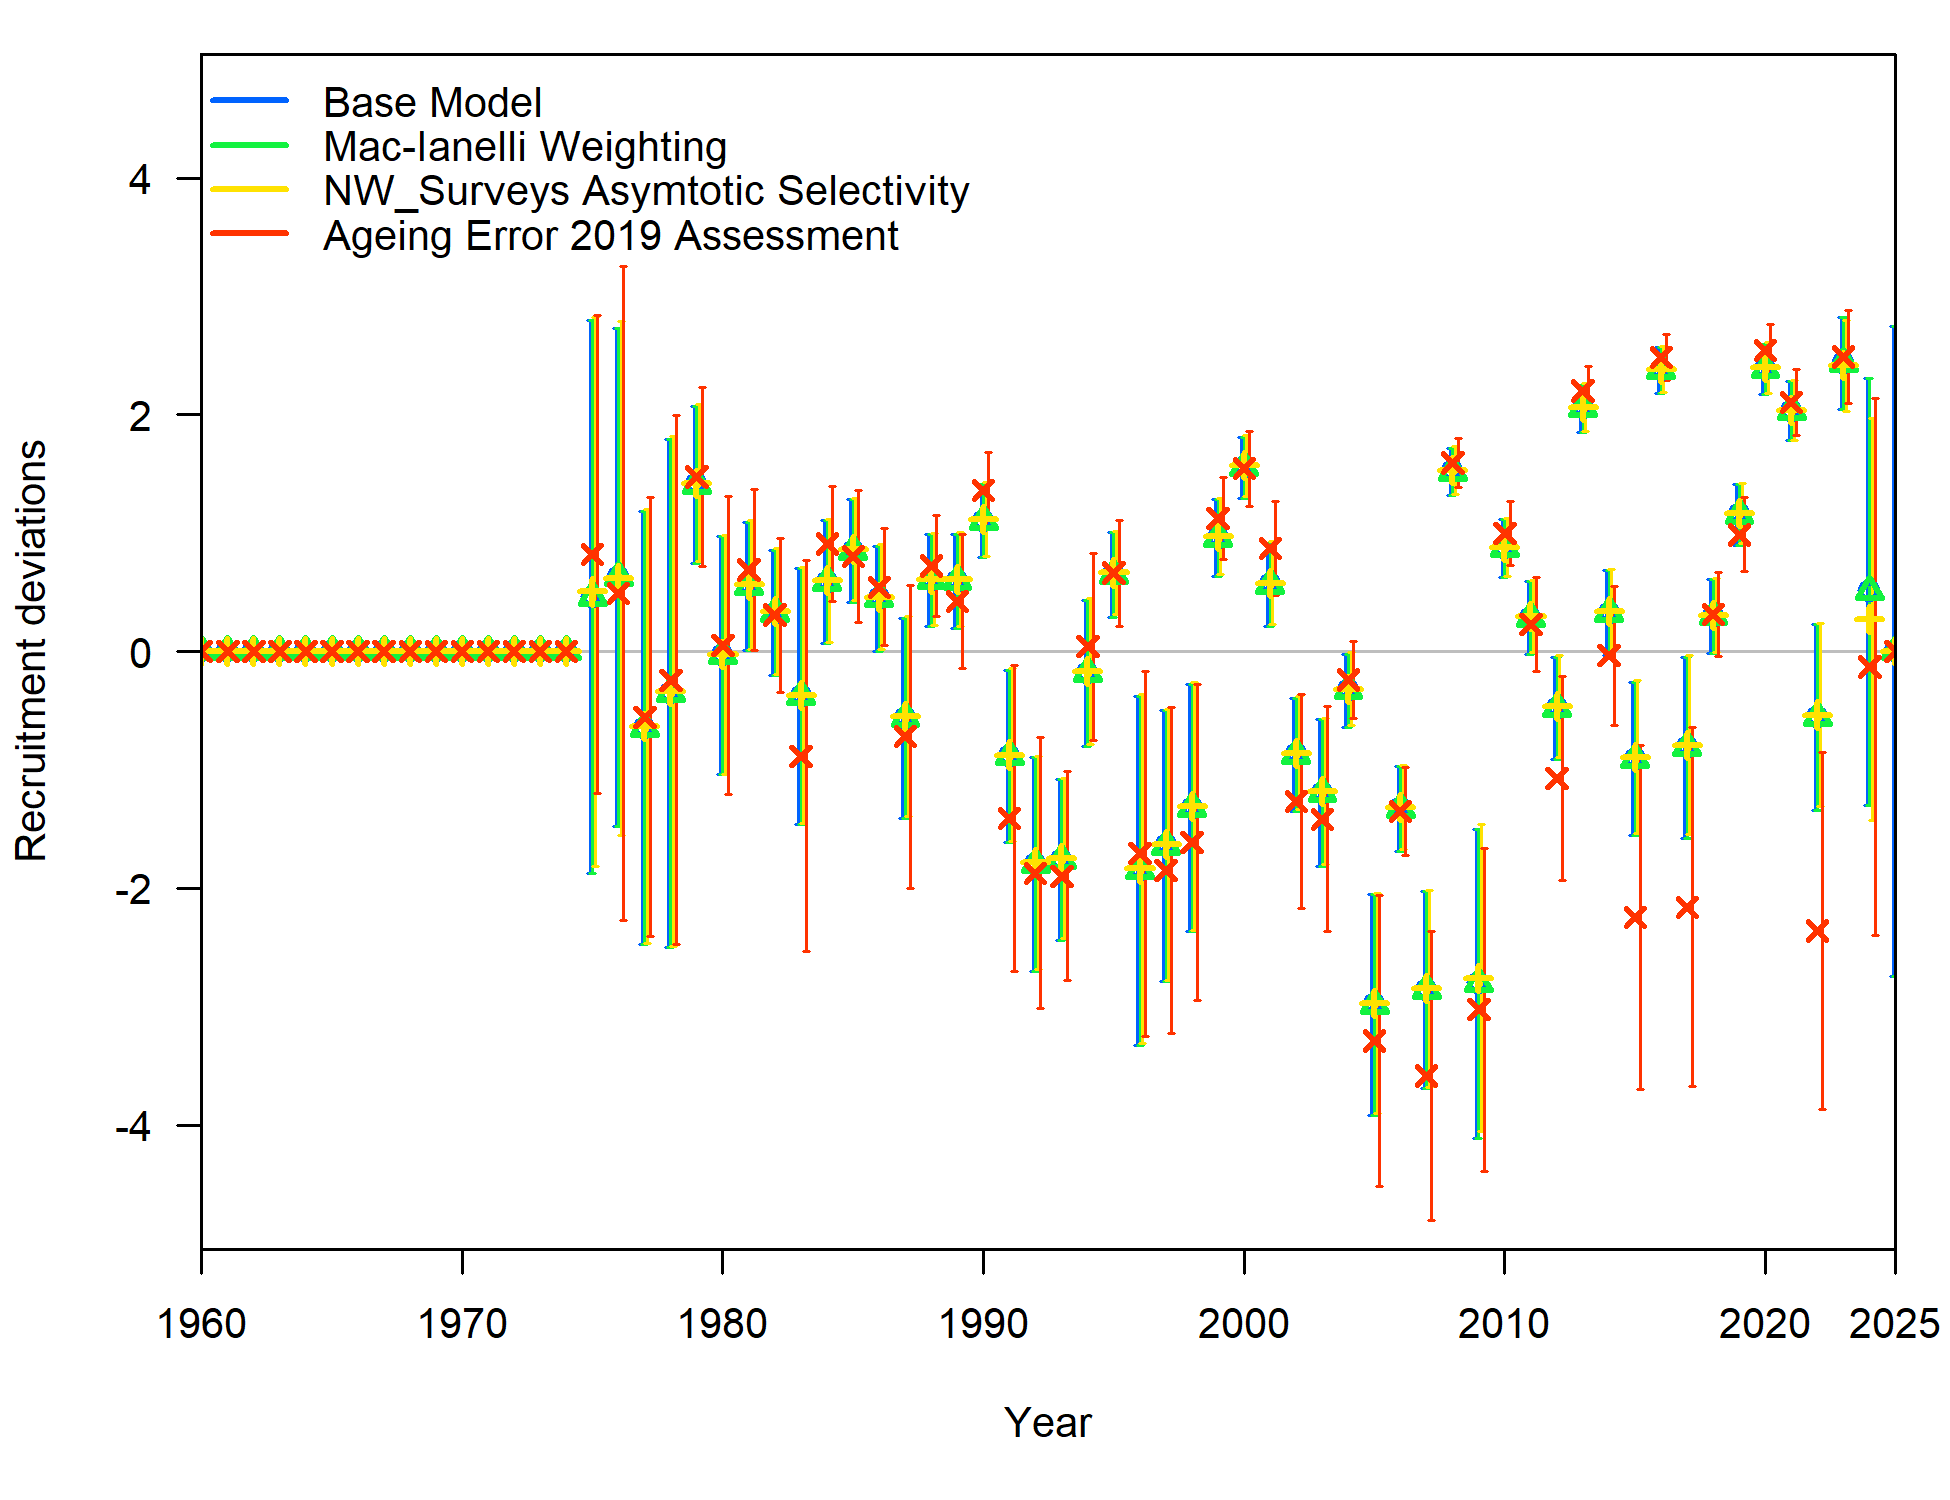
\includegraphics[width=1\linewidth,height=\textheight,keepaspectratio,alt={'Line plot with year on the x-axis and annual recruitment deviations in log-space on the y-axis. The estimated annual recruitment deviations from each sensitivity are similar to the base model, except for the sensitivity that uses the 2019 ageing error. The ageing error sensitiviy estimates more negative deviations for years with below average recruitment compared to the base model. Select parameters and derived quanties are provided in Table 35.'}]{figures/sens_2_compare12_recdevs_uncertainty.png}

}

\caption{\label{fig-sens-2-recdev}Maximum likelihood estimates of
recruitment deviations from 1960-2025 for the base model and alternative
sensitivity runs representing the use of the McAllister-Ianelli harmonic
mean method for weighting composition data, the specification of
asymptotic selectivity for NWFSC Surveys, and using the ageing error
vector applied in the 2019 stock assessment. Bars represent asymptotic
95 percent confidence intervals.}

\end{figure}%

\begin{figure}[H]

\centering{

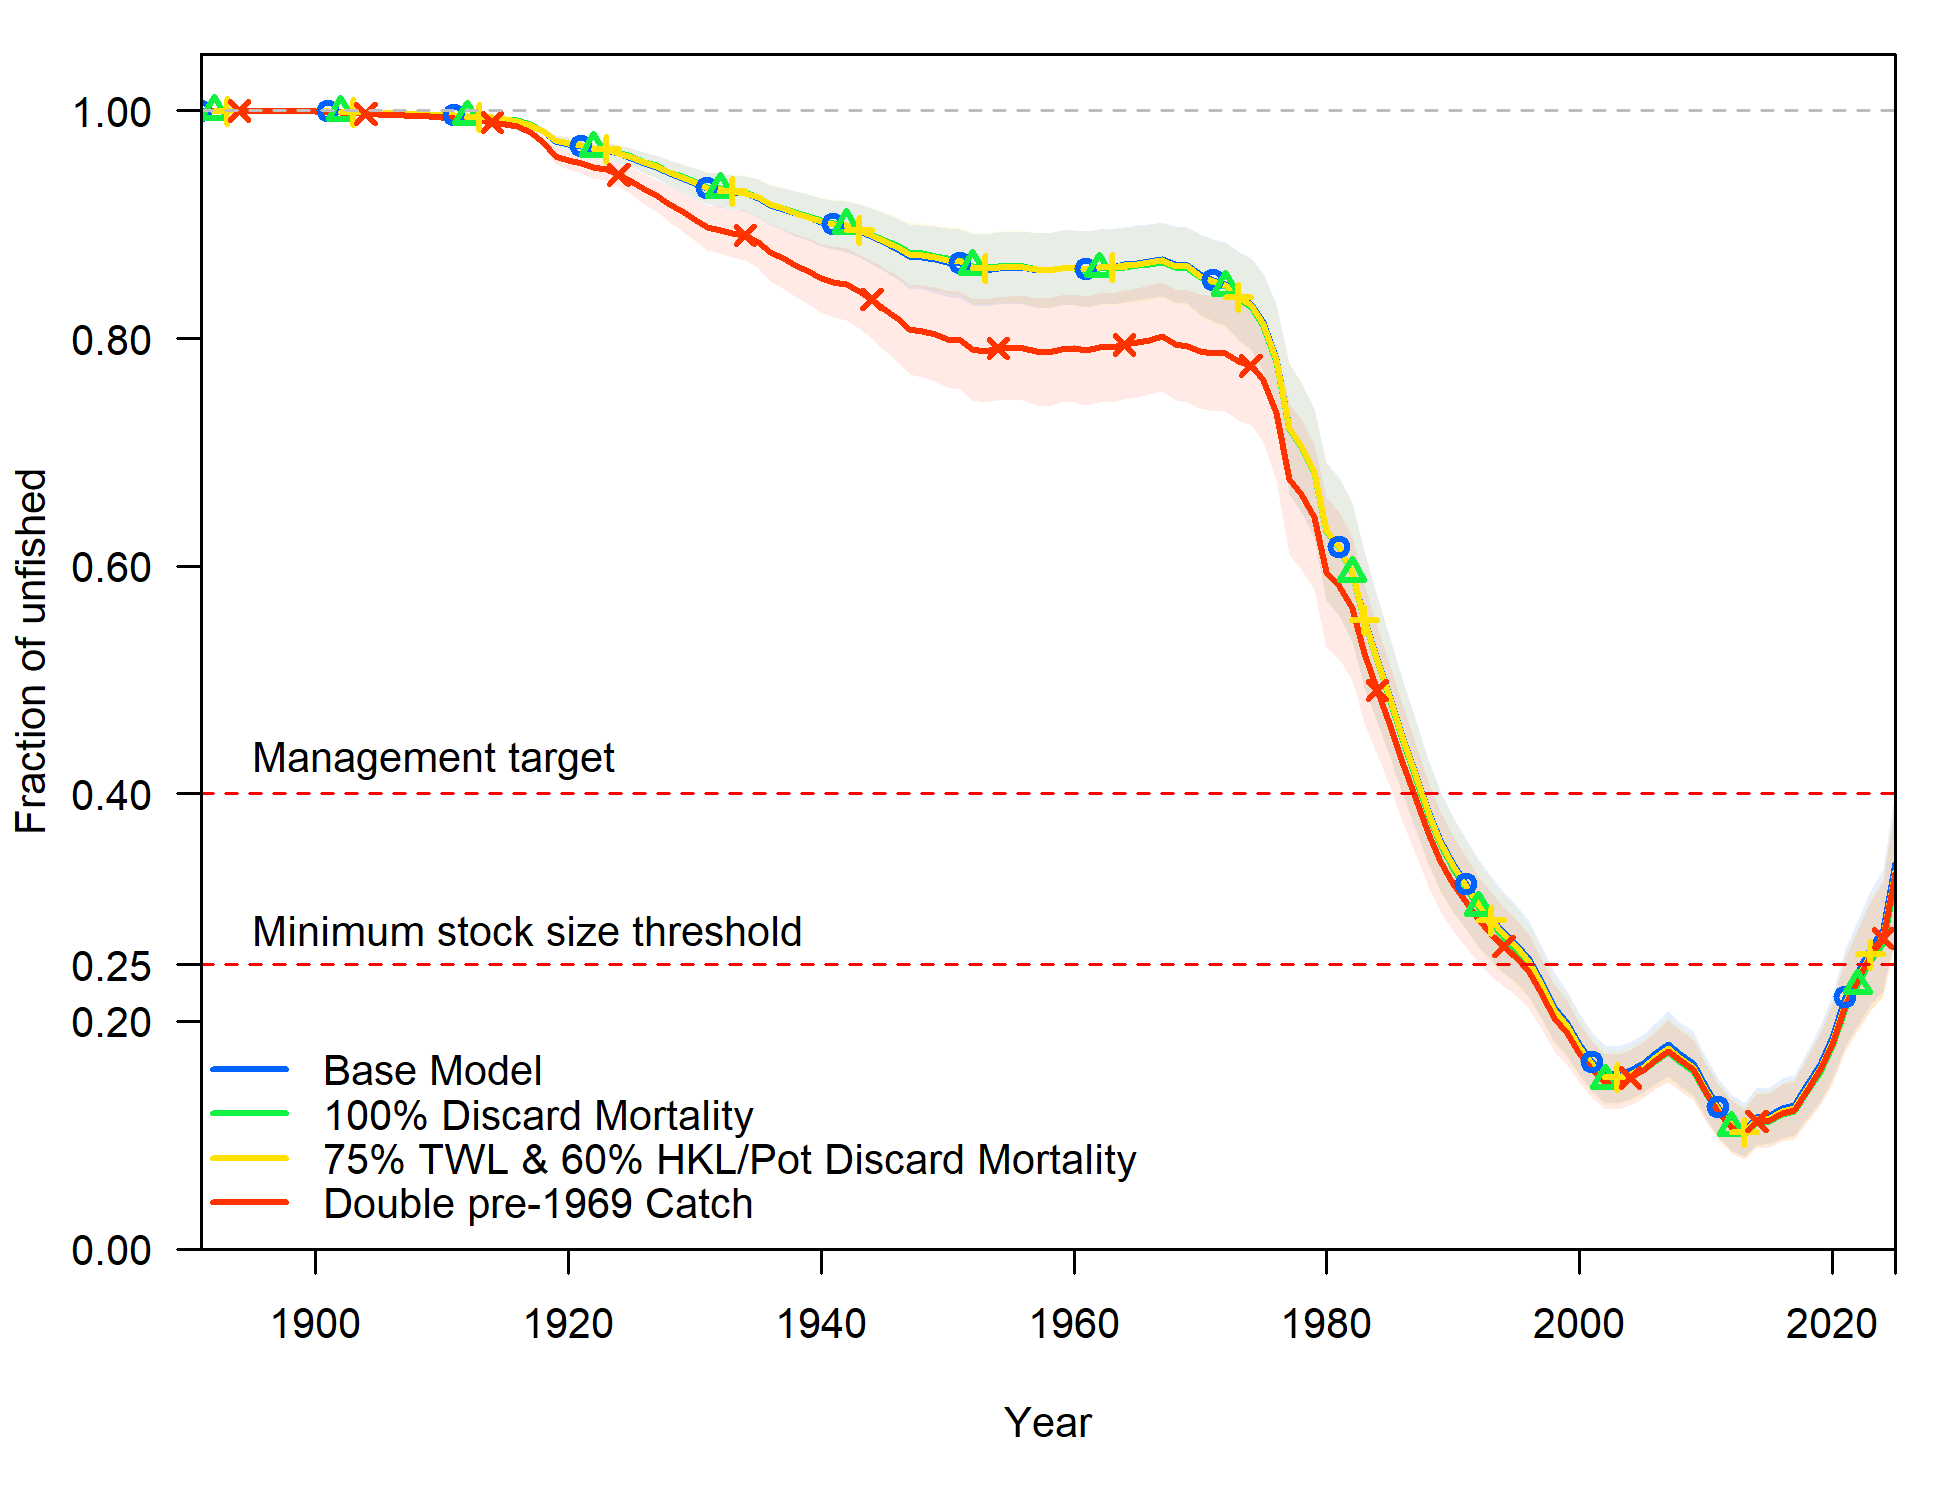
\includegraphics[width=1\linewidth,height=\textheight,keepaspectratio,alt={'Line plot with year on the x-axis and fraction of unfished on the y-axis. Each of the sensitivities has nearly identical trajectories compared to the base model, except for the sensitivity that doubled the pre-1969 catch. This sensitivity estimated a more depleted population from 1915 to 1980 compared to the base model. Select parameters and derived quanties are provided in Table 36.'}]{figures/sens_5_compare4_Bratio_uncertainty.png}

}

\caption{\label{fig-sens-5-bratio}Maximum likelihood estimates of
fraction of unfished (i.e., stock status) for the base model and
alternative sensitivity runs where discard mortality was increased to
100\% for all fleets, discard mortality was increased to 75\% for the
trawl fishery and 60\% for both hook-and-line and pot fisheries, and the
pre-1969 catch was doubled. Shaded regions represent asymptotic 95
percent confidence intervals.}

\end{figure}%

\begin{figure}[H]

\centering{

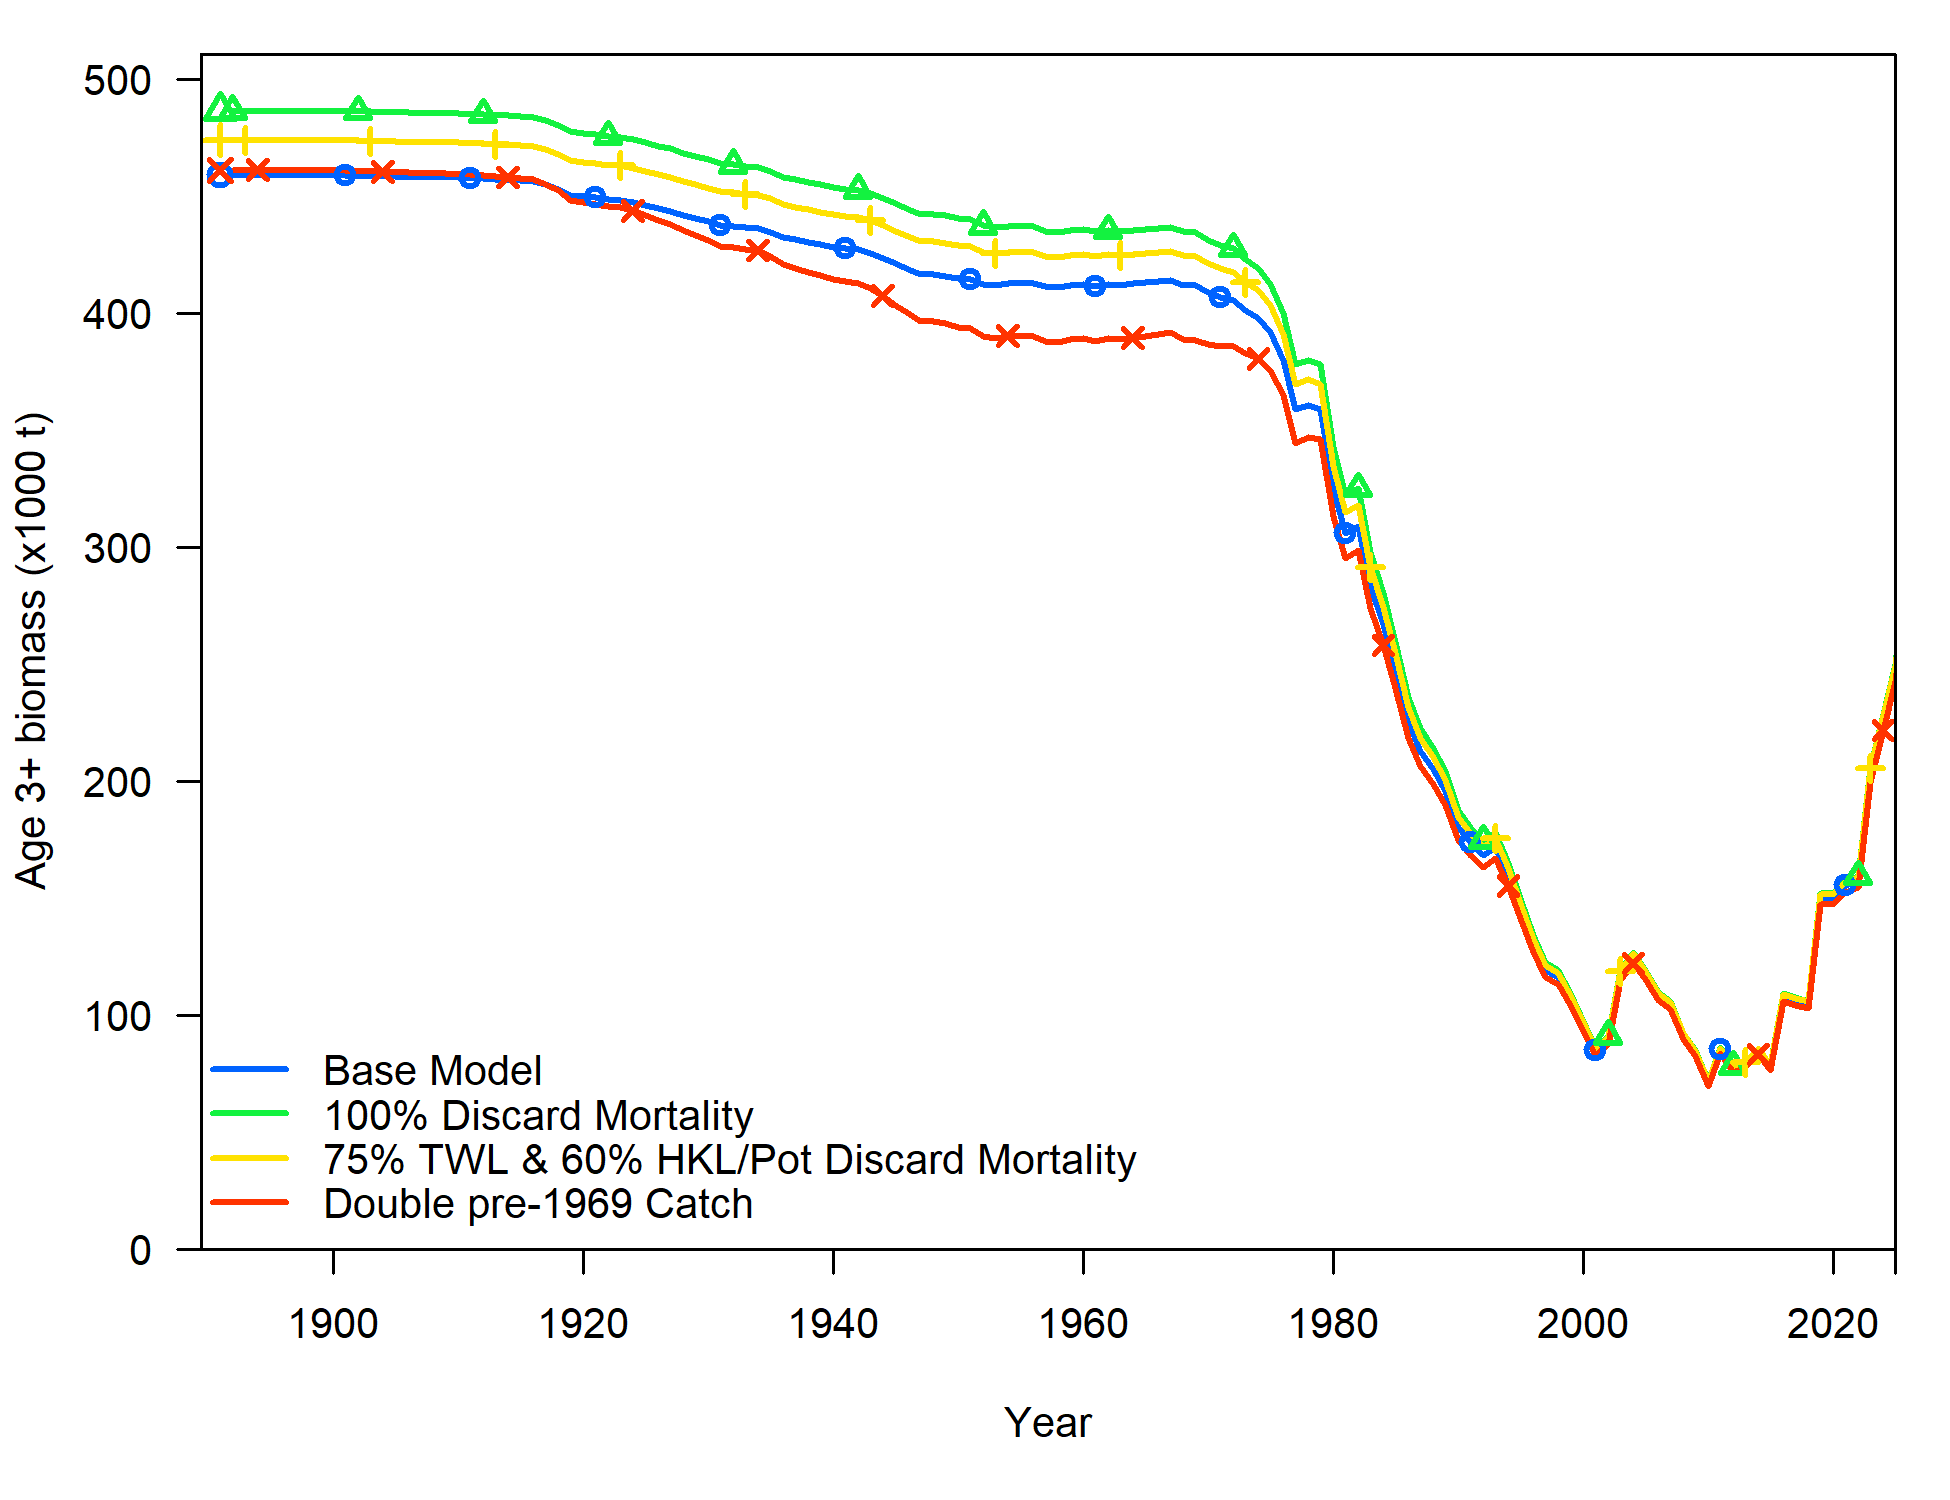
\includegraphics[width=1\linewidth,height=\textheight,keepaspectratio,alt={'Line plot with year on the x-axis and age 3 plus biomass on the y-axis. Each of the sensitivities has nearly identical trajectories compared to the base model from 1890 to 2025, except for the sensitivity that doubled the ore-1969 catches. There were with minor differences in the unfished age 3 plus biomass estimates for each of the sensitivities. Select parameters and derived quanties are provided in Table 36.'}]{figures/sens_5_compare18_smrybio.png}

}

\caption{\label{fig-sens-5-sumB}Maximum likelihood estimates of summary
biomass (age 3 and older) for the base model and alternative sensitivity
runs where discard mortality was increased to 100\% for all fleets,
discard mortality was increased to 75\% for the trawl fishery and 60\%
for both hook-and-line and pot fisheries, and the pre-1969 catch was
doubled.}

\end{figure}%

\begin{figure}[H]

\centering{

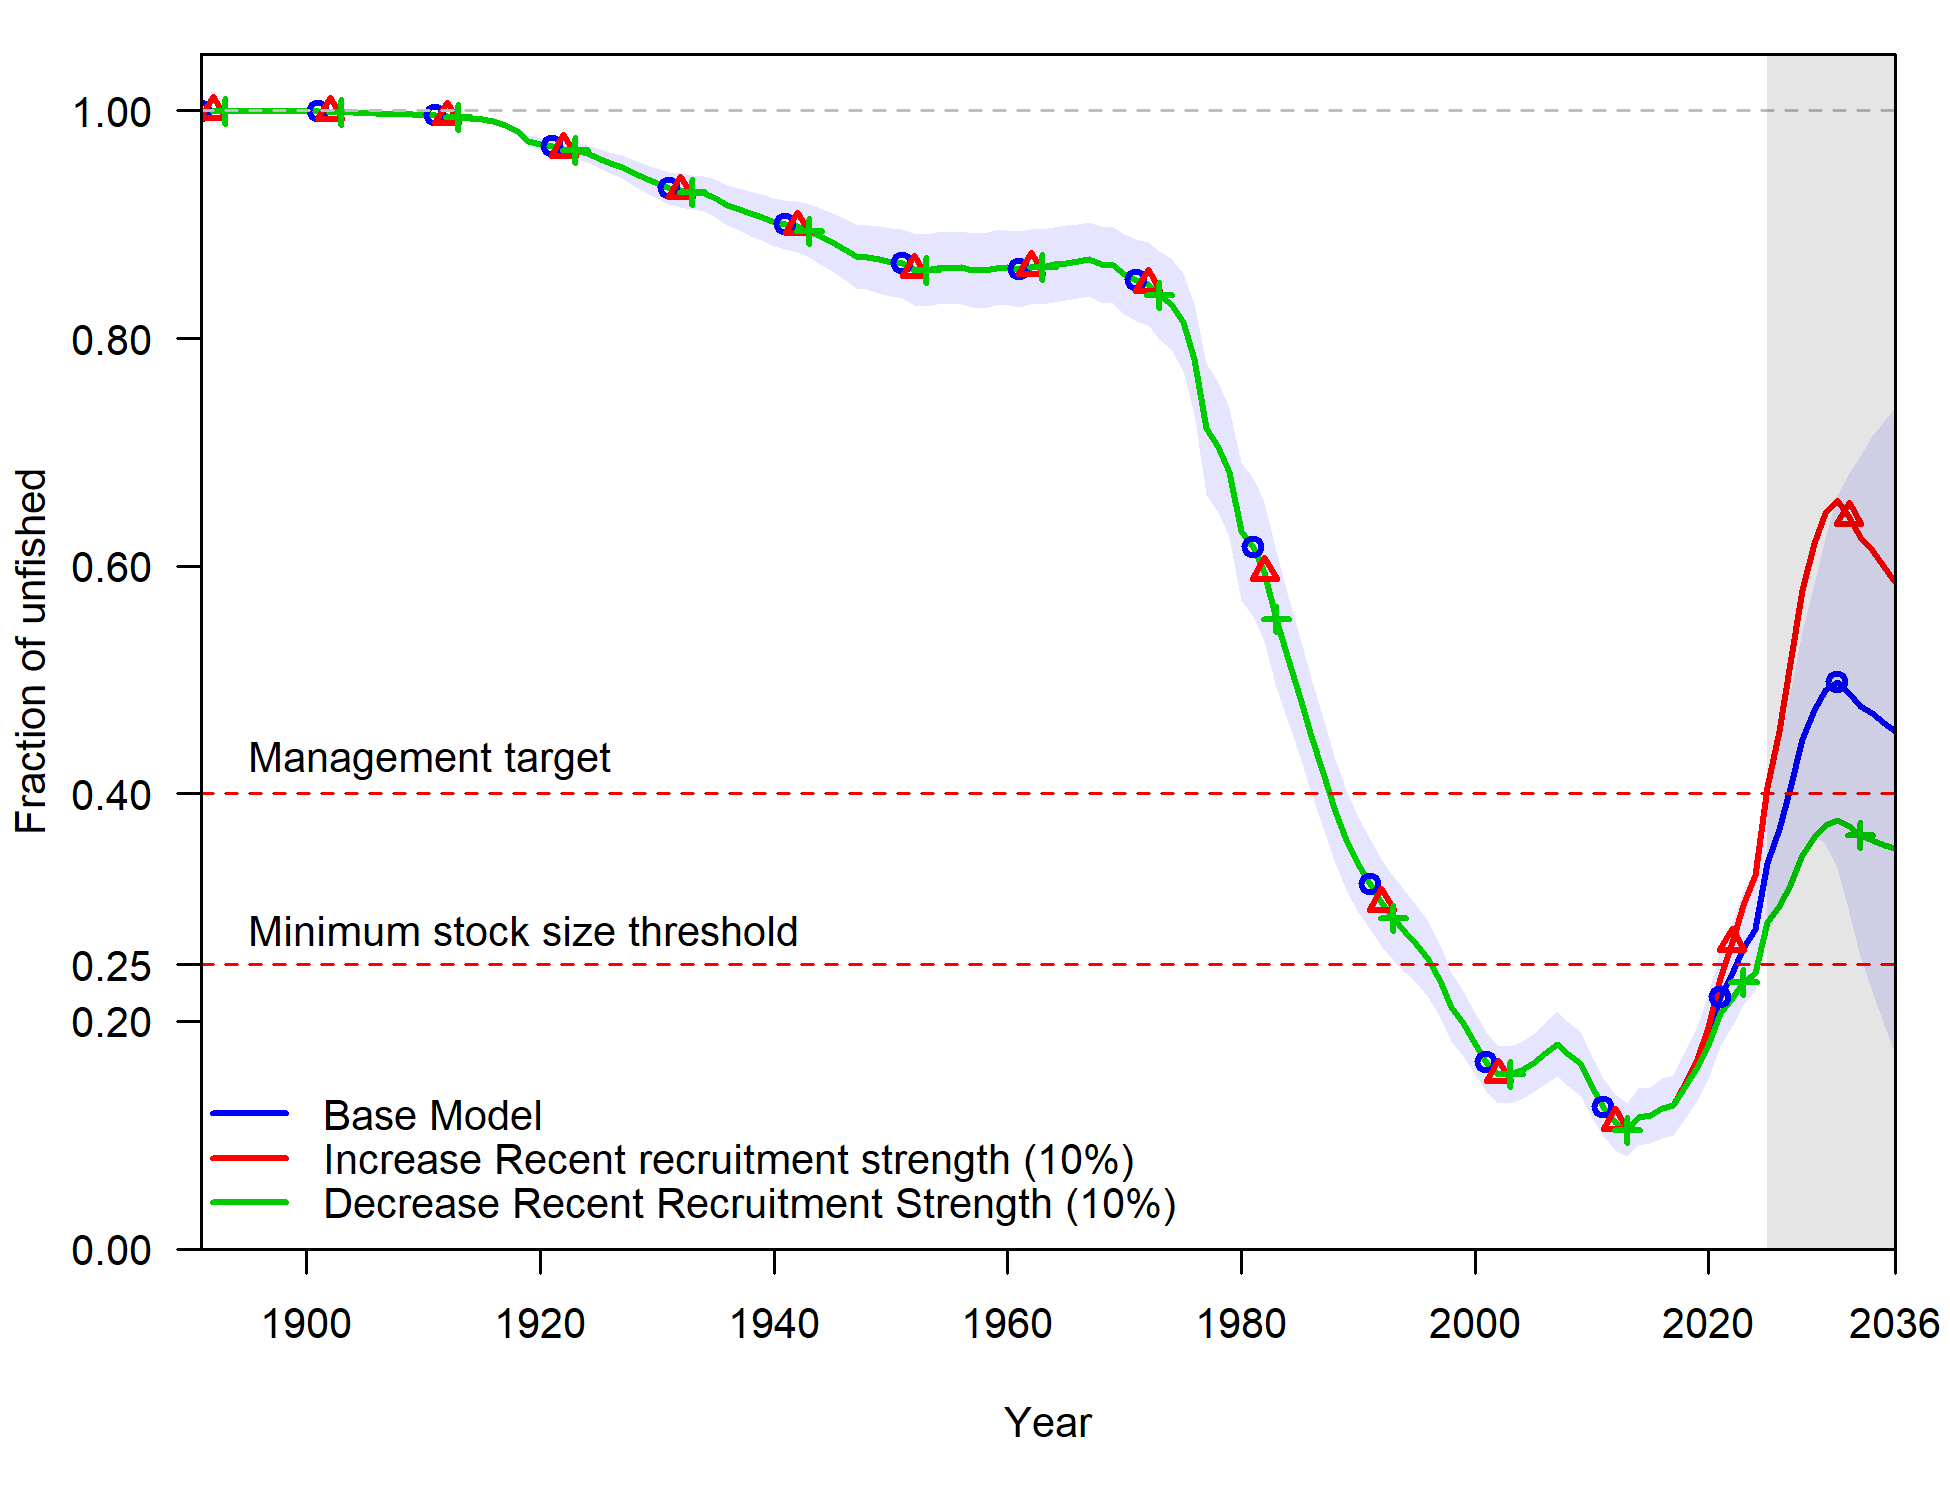
\includegraphics[width=1\linewidth,height=\textheight,keepaspectratio,alt={'Line plot with year on the x-axis and fraction of unfished on the y-axis. Each of the sensitivities has nearly identical trajectories compared to the base model from 1890 to 2018 and then diverge from the base model from 2019 to 2025. The sensitivity that assumed lower annual recruitment deviations in recent years resulted in a stock status of 0.287 in 2025. The sensitivity that assumed higher annual recruitment deviations in recent years resulted in a stock status of 0.406 in 2025. Select derived quanties are provided in Table 37.'}]{figures/sens_6_compare4_Bratio_uncertainty.png}

}

\caption{\label{fig-sens-6-bratio}Maximum likelihood estimates of
fraction of unfished (i.e., stock status) for the base model and
alternative sensitivity runs that either increase or decrease the
strength of recent (2016-2023) recruitment deviations by 10\% in
log-space. Sensitivity models were run with all model parameters fixed
at the base model maximum likelihood estimates, with the only changes
being from the specified adjustments to recent recruitment deviations.
Forecast catches in 2025 and 2026 were based on GMT recommendations. The
catches from 2027 to 2036 were set equal to the year-specific ABCs. The
shaded regions represents the asymptotic 95 percent confidence interval
for the base model.}

\end{figure}%

\begin{figure}[H]

\centering{

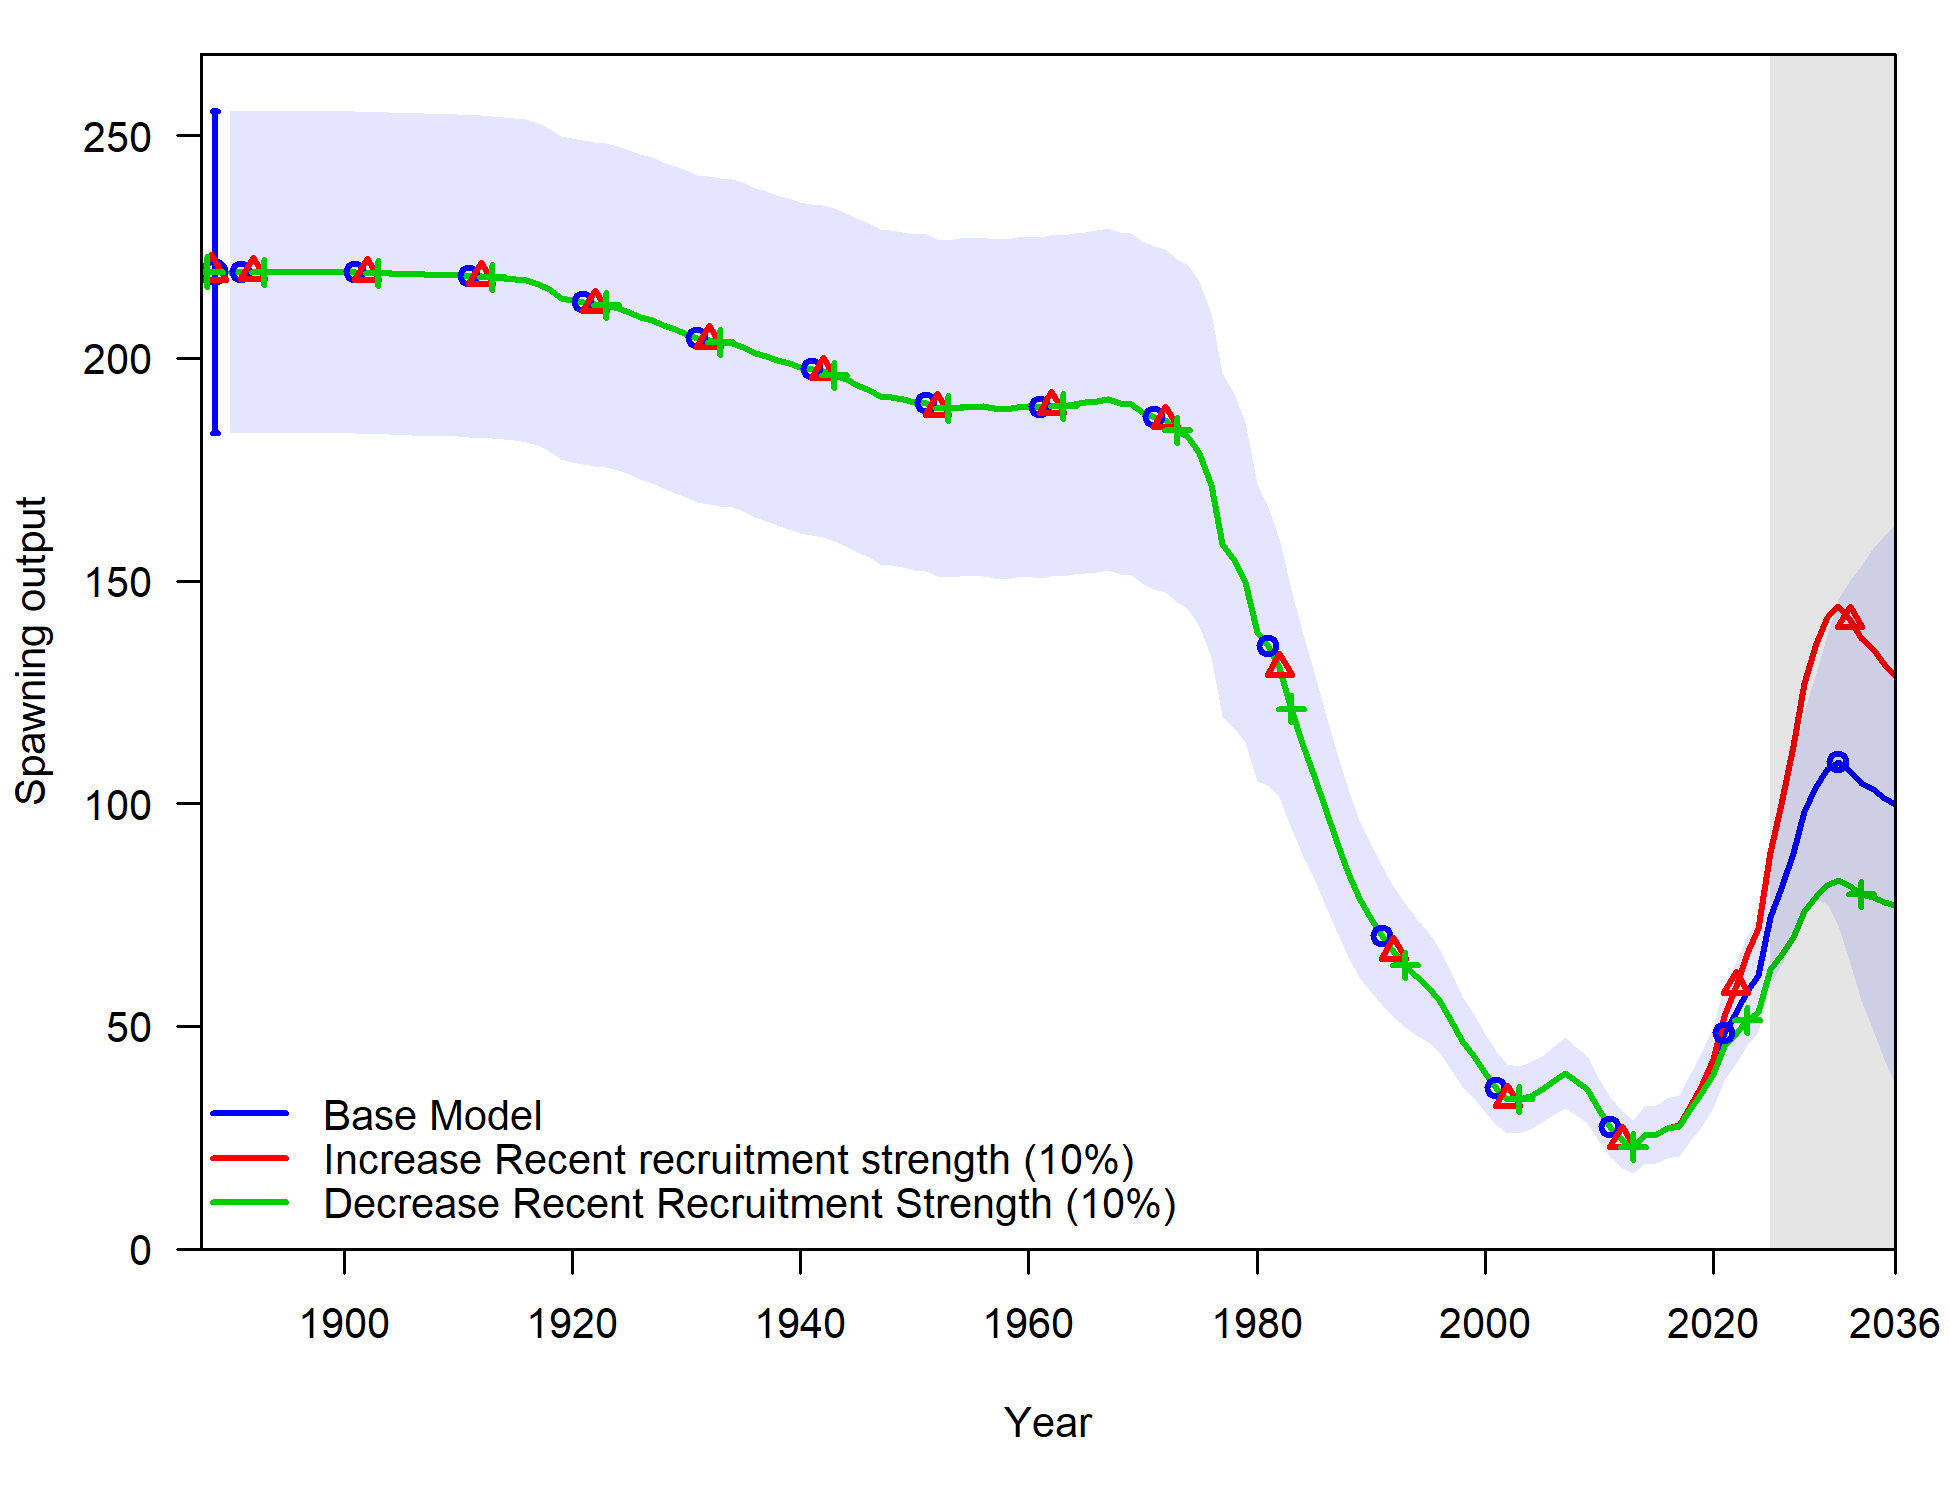
\includegraphics[width=1\linewidth,height=\textheight,keepaspectratio,alt={'Line plot with year on the x-axis and spawning biomass on the y-axis. Each of the sensitivities has nearly identical trajectories compared to the base model from 1890 to 2018 and then diverge from the base model from 2019 to 2025. The sensitivity that assumed lower annual recruitment deviations in recent years resulted in spawning biomass around 62,881 metric tons in 2025. The sensitivity that assumed higher annual recruitment deviations in recent years resulted in spawning biomass around 89,012 metric tons in 2025. Select derived quanties are provided in Table 37.'}]{figures/sens_6_compare2_spawnbio_uncertainty.png}

}

\caption{\label{fig-sens-6-ssb}Maximum likelihood estimates of spawning
biomass for the base model and alternative sensitivity runs that either
increase or decrease the strength of recent (2016-2023) recruitment
deviations by 10\% in log-space. Sensitivity models were run with all
model parameters fixed at the base model maximum likelihood estimates,
with the only changes being from the specified adjustments to recent
recruitment deviations. Forecast catches in 2025 and 2026 were based on
GMT recommendations. The catches from 2027 to 2036 were set equal to the
year-specific ABCs. The shaded regions represents the asymptotic 95
percent confidence interval for the base model.}

\end{figure}%

\subsection{Likelihood Profiles}\label{likelihood-profiles}

\begin{figure}[H]

\centering{

\includegraphics[width=1\linewidth,height=\textheight,keepaspectratio,alt={'Three panel plot with log(R0) on the x-axis and change in log-likelihood on the y-axis with panels showing the contribution from each data type in the model, the contribution from age data from each fleet, and the survey data from each survey fleet. The age data is the primarily source of information informing the estimate of log(R0) with age data from the trawl fleet supporting higher log(R0) and the pot fleet supporting lower values. There  is little to no information about log(R0) from the survey indices.'}]{../model/base_model/8.36_base_model_profile_SR_LN(R0)/piner_panel_SR_LN(R0).png}

}

\caption{\label{fig-r0-profile}Change in the negative log-likelihood
across a range of log(\emph{R\textsubscript{0})} values.}

\end{figure}%

\begin{figure}[H]

\centering{

\includegraphics[width=1\linewidth,height=\textheight,keepaspectratio,alt={'Line plot with year on the x-axis and spawning output on the y-axis which multiple model runs that assume a range of log(R0) values.'}]{../model/base_model/8.36_base_model_profile_SR_LN(R0)/SR_LN(R0)_trajectories_compare1_spawnbio.png}

}

\caption{\label{fig-r0-profile-ssb}Change in the spawning output across
a range of log(\emph{R\textsubscript{0})} values.}

\end{figure}%

\begin{figure}[H]

\centering{

\includegraphics[width=1\linewidth,height=\textheight,keepaspectratio,alt={'Line plot with year on the x-axis and fraction of unfished on the y-axis with multiple model runs that assume a range of log(R0) values.'}]{../model/base_model/8.36_base_model_profile_SR_LN(R0)/SR_LN(R0)_trajectories_compare3_Bratio.png}

}

\caption{\label{fig-r0-profile-depl}Change in the fraction of unfished
(i.e., stock status) across a range of log(\emph{R\textsubscript{0})}
values.}

\end{figure}%

\begin{figure}[H]

\centering{

\includegraphics[width=1\linewidth,height=\textheight,keepaspectratio,alt={'Three panel plot with natural mortality on the x-axis and change in log-likelihood on the y-axis with panels showing the contribution from each data type in the model, the contribution from age data from each fleet, and the survey data from each survey fleet. The age data is the primarily source of information informing the estimate of natural mortality with age data from the trawl fleet supporting higher natural mortality values and the WCGBTS age data supporting lower values. There  is little to no information about log(R0) from the survey indices.'}]{../model/base_model/8.36_base_model_profile_NatM_uniform_Fem_GP_1/piner_panel_NatM_uniform_Fem_GP_1.png}

}

\caption{\label{fig-m-profile}Change in the negative log-likelihood
across a range of natural mortality (\emph{M}) values. Only female
\emph{M} is shown, because \emph{M} is sex-invariant in the base model.}

\end{figure}%

\begin{figure}[H]

\centering{

\includegraphics[width=1\linewidth,height=\textheight,keepaspectratio,alt={'Line plot with year on the x-axis and spawning output on the y-axis which multiple model runs that assume a range of natural mortality values.'}]{../model/base_model/8.36_base_model_profile_NatM_uniform_Fem_GP_1/NatM_uniform_Fem_GP_1_trajectories_compare1_spawnbio.png}

}

\caption{\label{fig-m-profile-ssb}Change in the spawning output across a
range of natural mortality (\emph{M}) values. Only female \emph{M} is
shown, because \emph{M} is sex-invariant in the base model.}

\end{figure}%

\begin{figure}[H]

\centering{

\includegraphics[width=1\linewidth,height=\textheight,keepaspectratio,alt={'Line plot with year on the x-axis and fraction of unfished on the y-axis which multiple model runs that assume a range of natural mortality values.'}]{../model/base_model/8.36_base_model_profile_NatM_uniform_Fem_GP_1/NatM_uniform_Fem_GP_1_trajectories_compare3_Bratio.png}

}

\caption{\label{fig-m-profile-depl}Change in the fraction of unfished
(i.e., stock status) across a range of natural mortality (\emph{M})
values. Only female \emph{M} is shown, because \emph{M} is sex-invariant
in the base model.}

\end{figure}%

\begin{figure}[H]

\centering{

\includegraphics[width=1\linewidth,height=\textheight,keepaspectratio,alt={'Three panel plot with steepness on the x-axis and change in log-likelihood on the y-axis with panels showing the contribution from each data type in the model, the contribution from age data from each fleet, and the survey data from each survey fleet. There  is little to no information about steepness in each data type.'}]{../model/base_model/8.36_base_model_profile_SR_BH_steep/piner_panel_SR_BH_steep.png}

}

\caption{\label{fig-h-profile}Change in the negative log-likelihood
across a range of steepness (\emph{h}) values.}

\end{figure}%

\begin{figure}[H]

\centering{

\includegraphics[width=1\linewidth,height=\textheight,keepaspectratio,alt={'Line plot with year on the x-axis and spawning output on the y-axis which multiple model runs that assume a range of steepness values.'}]{../model/base_model/8.36_base_model_profile_SR_BH_steep/SR_BH_steep_trajectories_compare1_spawnbio.png}

}

\caption{\label{fig-h-profile-ssb}Change in the spawning output across a
range of steepness (\emph{h}) values.}

\end{figure}%

\begin{figure}[H]

\centering{

\includegraphics[width=1\linewidth,height=\textheight,keepaspectratio,alt={'Line plot with year on the x-axis and fraction of unfished on the y-axis which multiple model runs that assume a range of steepness values.'}]{../model/base_model/8.36_base_model_profile_SR_BH_steep/SR_BH_steep_trajectories_compare3_Bratio.png}

}

\caption{\label{fig-h-profile-depl}Change in the fraction of unfished
(i.e., stock status) across a range of steepness (\emph{h}) values.}

\end{figure}%

\subsection{Retrospecitve Analysis}\label{retrospecitve-analysis}

\begin{figure}[H]

\centering{

\includegraphics[width=1\linewidth,height=\textheight,keepaspectratio,alt={'Line plot with year on the x-axis and spawning output on the y-axis with multiple runs that peel off one to ten years of recent data. The trajectories when data are peeled off are similar to the base model.'}]{../model/base_model/8.36_base_model_retro_10_yr_peel/compare2_spawnbio_uncertainty.png}

}

\caption{\label{fig-retro-sb}Change in the estimate of spawning output
when the most recent 10 years of data are removed sequentially.}

\end{figure}%

\begin{figure}[H]

\centering{

\includegraphics[width=1\linewidth,height=\textheight,keepaspectratio,alt={'Line plot with year on the x-axis and fraction of unfished on the y-axis with multiple runs that peel off one to ten years of recent data. The trajectories when data are peeled off are similar to the base model.'}]{../model/base_model/8.36_base_model_retro_10_yr_peel/compare4_Bratio_uncertainty.png}

}

\caption{\label{fig-retro-depl}Change in the estimate of fraction
unfished (i.e., stock status) when the most recent 10 years of data are
removed sequentially.}

\end{figure}%

\begin{figure}[H]

\centering{

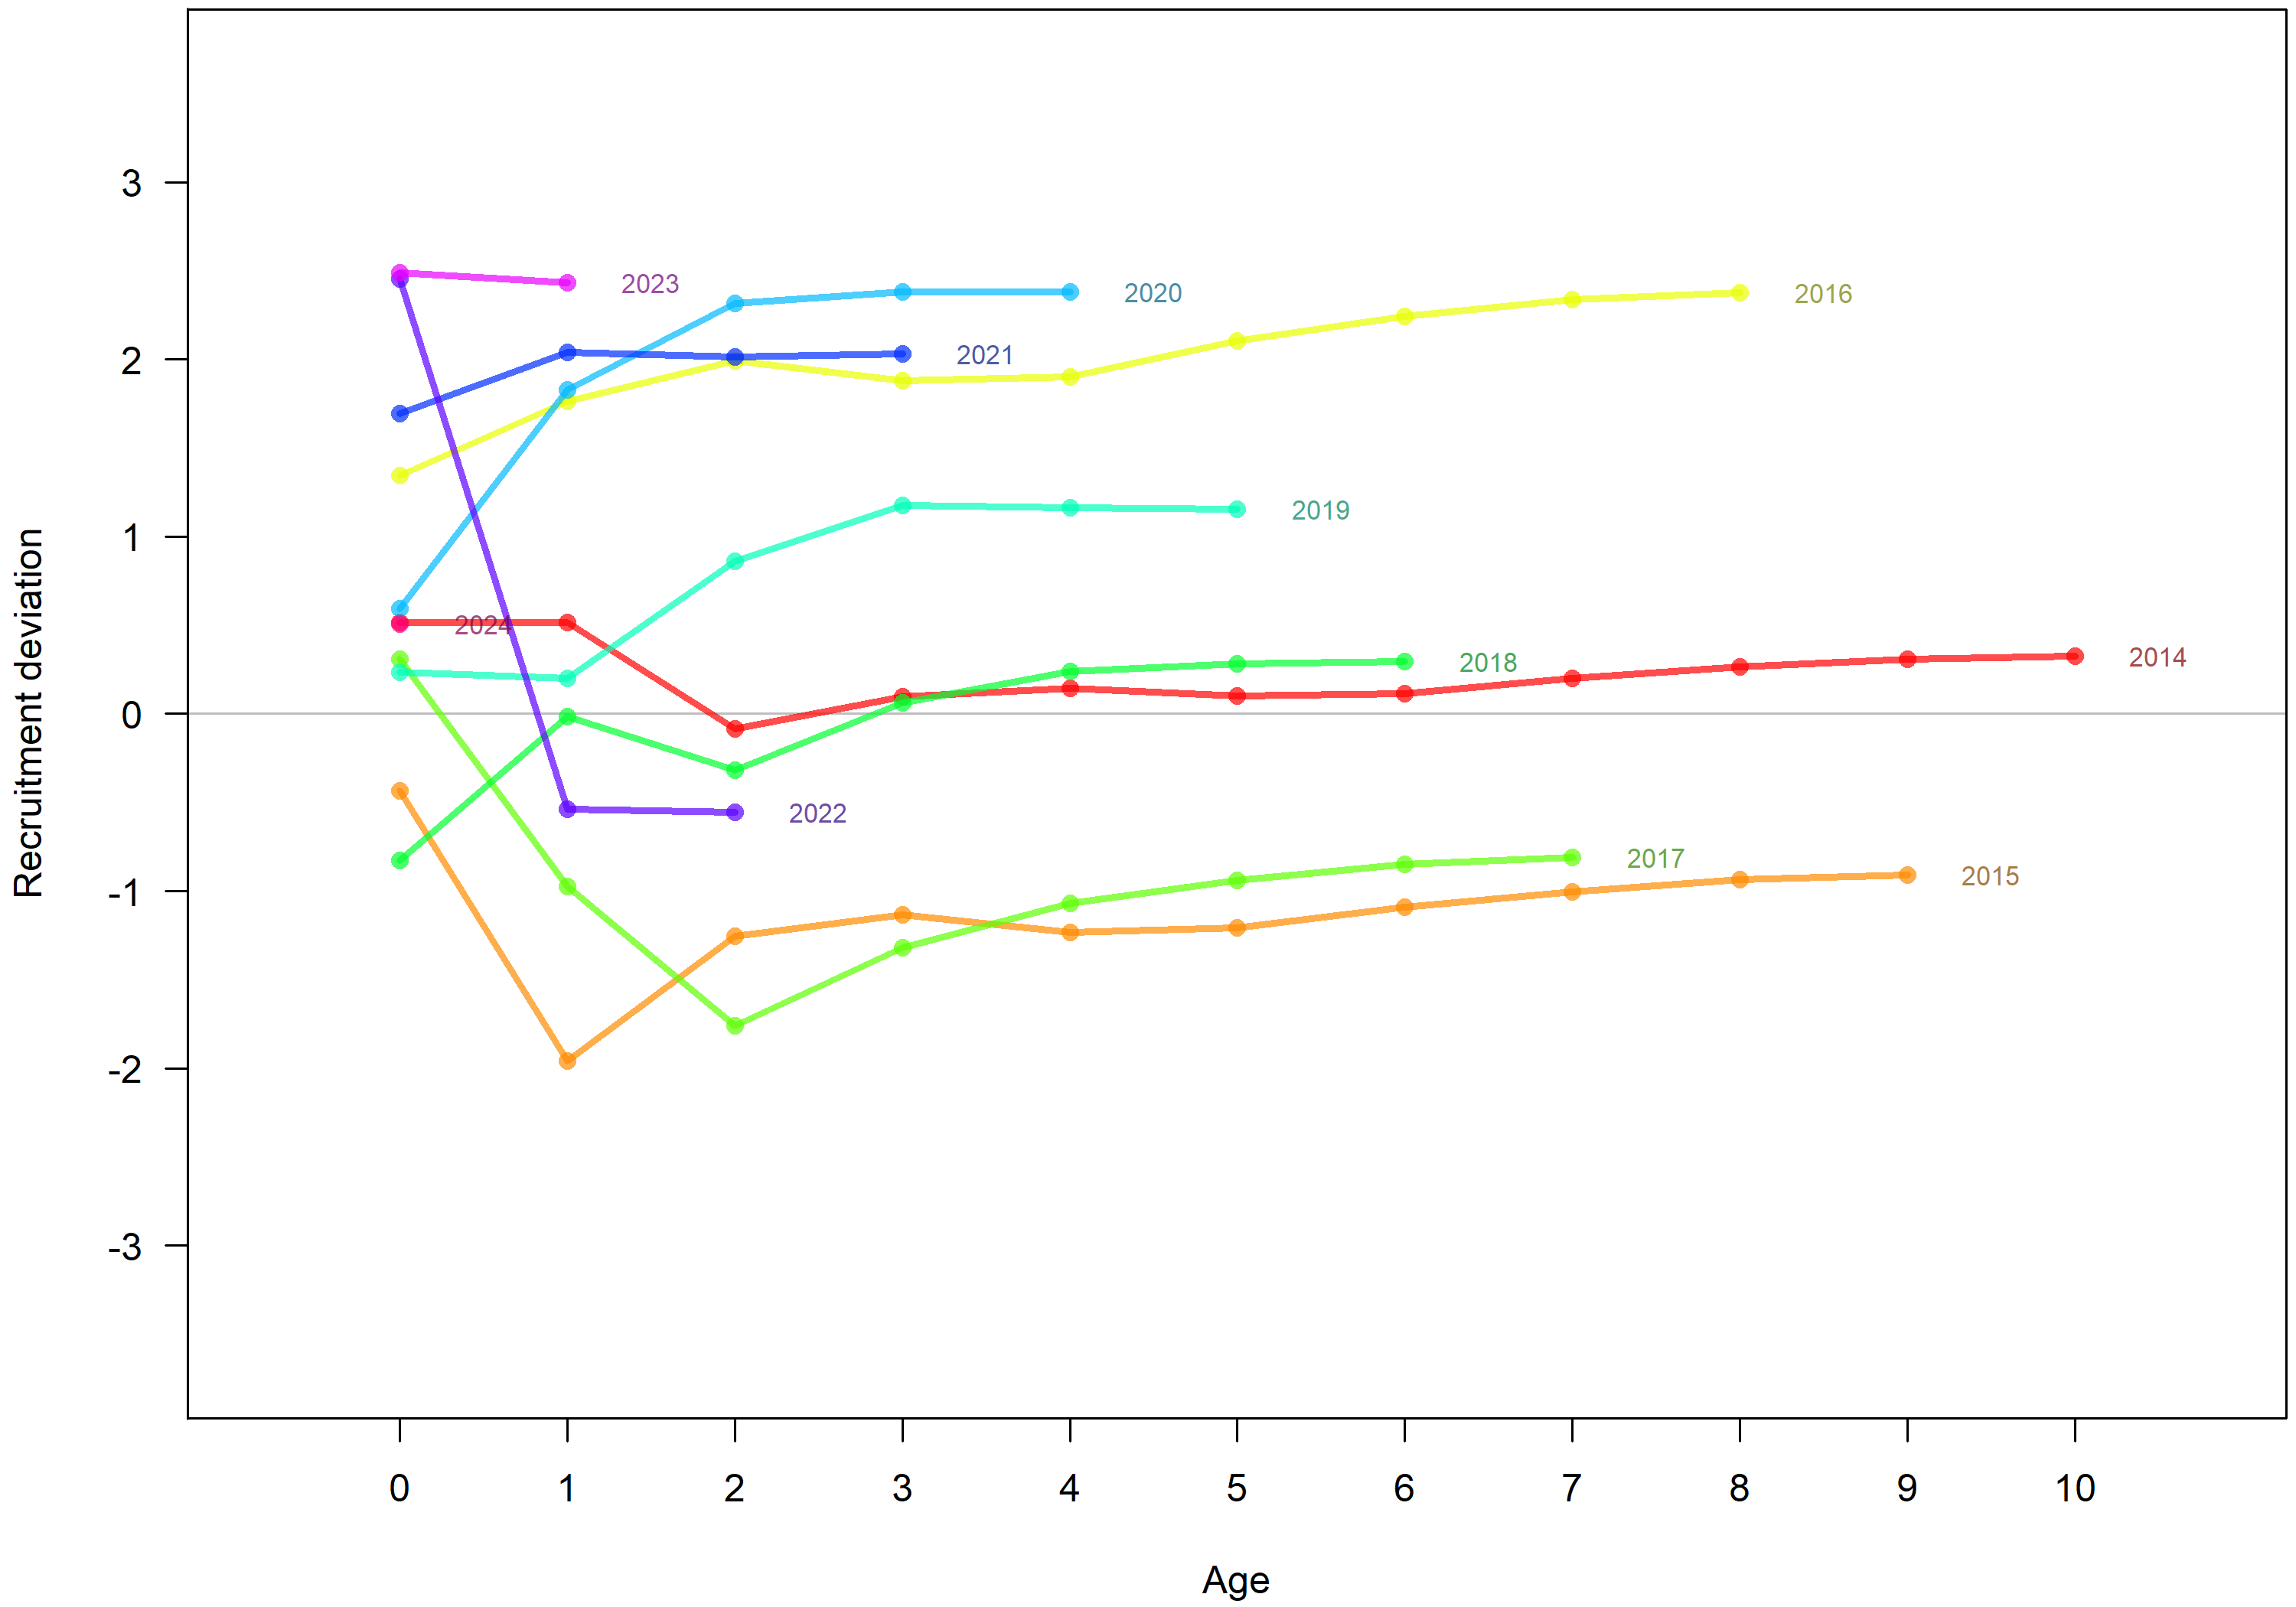
\includegraphics[width=1\linewidth,height=\textheight,keepaspectratio,alt={'Line plot with age from 0 to 10 on the x-axis and recruitment deviation in log-space on the y-axis. The estimates of recruitment deviations generally stabilize after 2 to 3 observations in the data.'}]{figures/recruitment_retrospective_squid_alternative.png}

}

\caption{\label{fig-squid-plot}Change in the estimate annual recruitment
deviations when the most recent 10 years of data are removed
sequentially.}

\end{figure}%

\subsection{Historical Analysis}\label{historical-analysis}

\begin{figure}[H]

\centering{

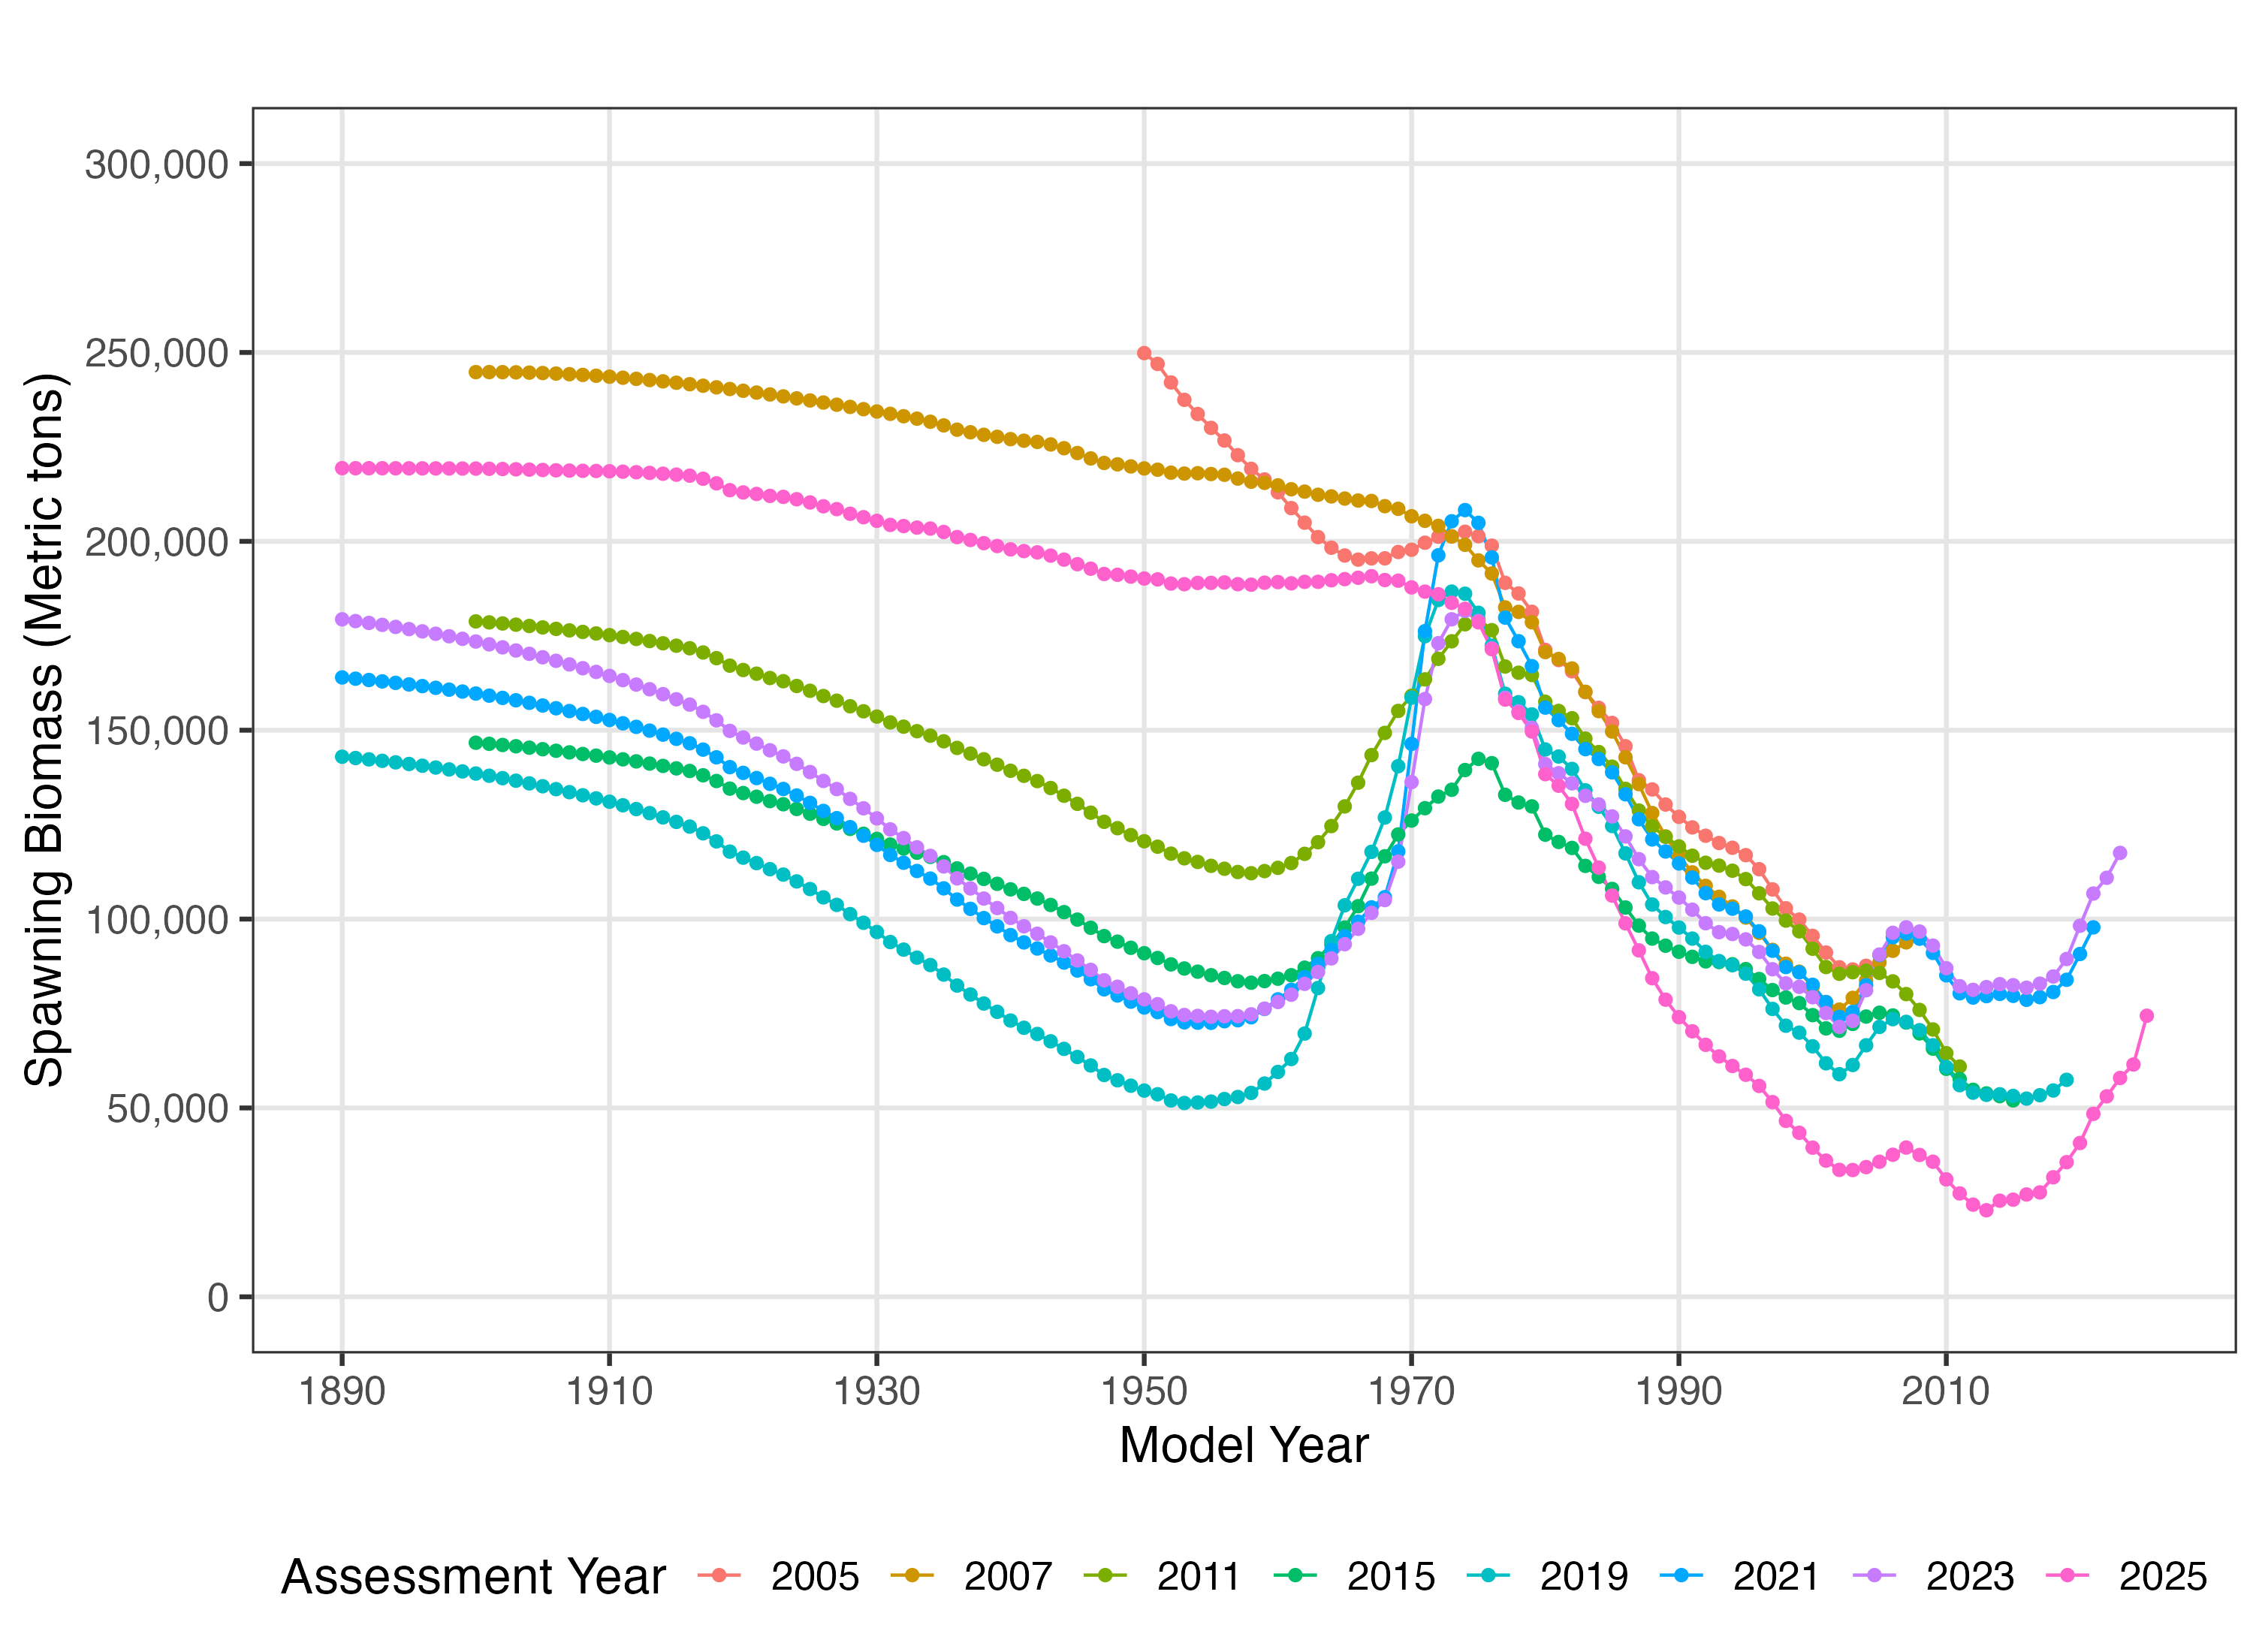
\includegraphics[width=1\linewidth,height=\textheight,keepaspectratio,alt={'Line plot with year on the x-axis and spawning output on the y-axis with the spawning output estimated from the 2005, 2007, 2011, 2015, 2019, 2021, 2023, and 2025 assessments of sablefish. Each of the assessments estimate a similar decline in spawning output from 1972 and beyond, but the 2025 assessment estimates lower spawning output from 1972 to 2025 compared to the previous assessments.'}]{figures/historical_ssb.png}

}

\caption{\label{fig-historical-ssb}Spawning ouptut (mt) trajectories
from the base model and historical assessments for sablefish.}

\end{figure}%

\begin{figure}[H]

\centering{

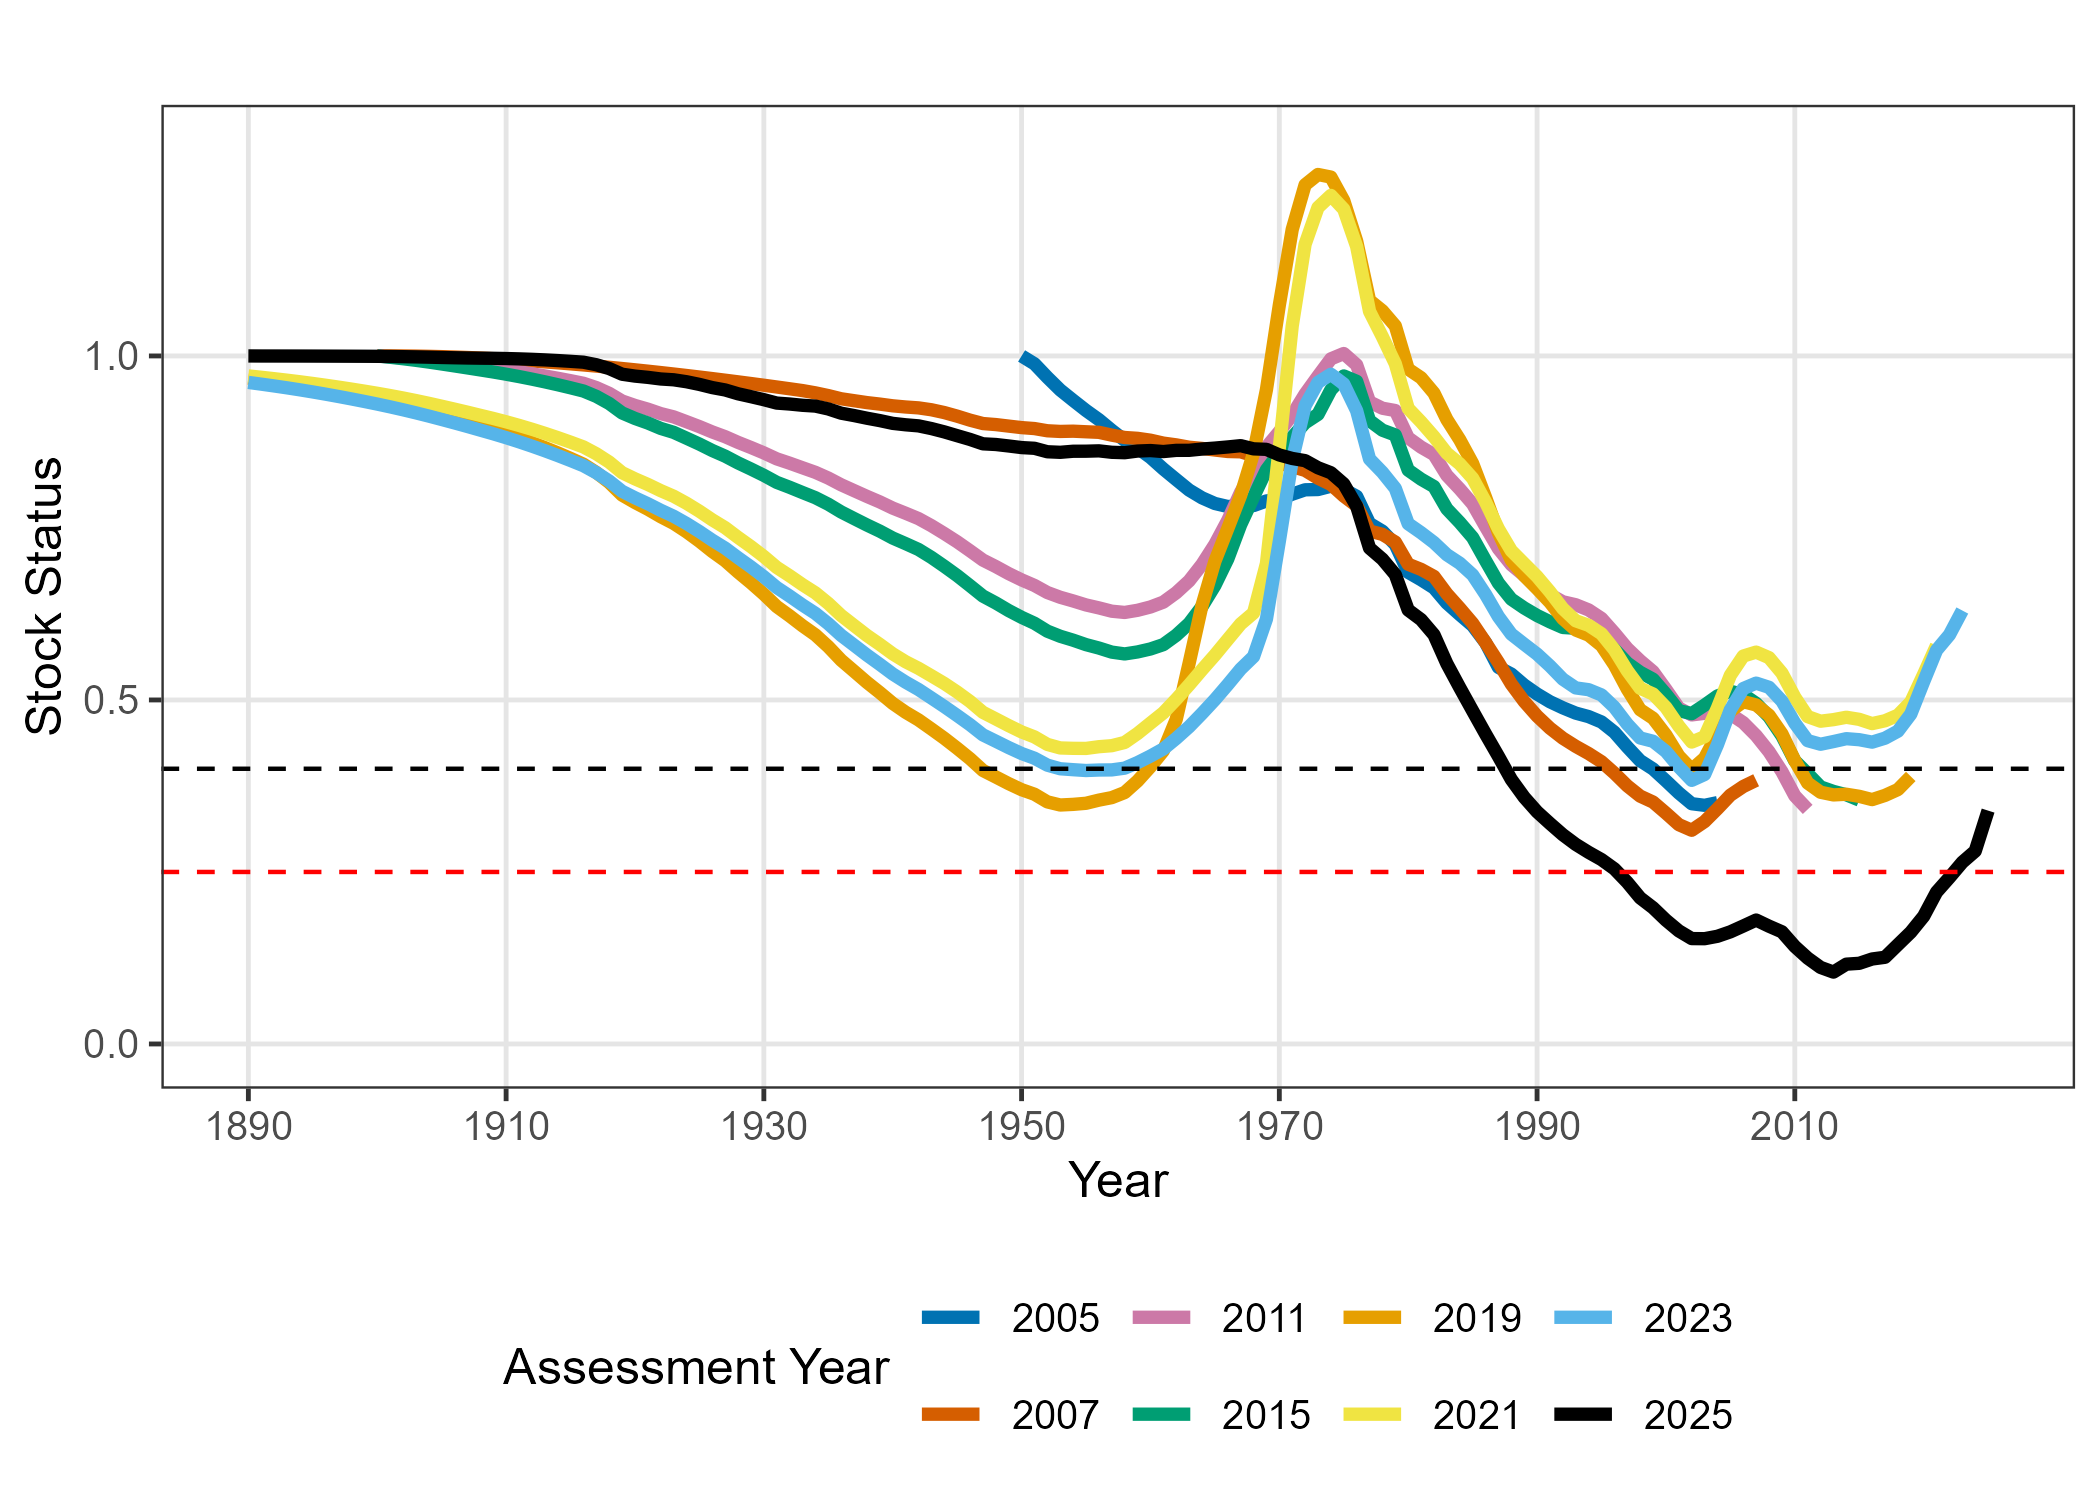
\includegraphics[width=1\linewidth,height=\textheight,keepaspectratio,alt={'Line plot with year on the x-axis and stock status on the y-axis with the stock status estimated from the 2005, 2007, 2011, 2015, 2019, 2021, 2023, and 2025 assessments of sablefish. Each of the assessments estimate a similar decline in stock status from 1972 and beyond, but the 2025 assessment estimates a more depleted population from 1972 to 2025 compared to the previous assessments.'}]{figures/historical_depl.png}

}

\caption{\label{fig-historical-depl}Stock status trajectories from the
base model and historical assessments for sablefish.}

\end{figure}%

\subsection{Management}\label{management-1}

\begin{figure}[H]

\centering{

\includegraphics[width=1\linewidth,height=\textheight,keepaspectratio,alt={'Line plot with year on the x-axis and relative fishing intensity on the y-axis.  The relative fishing intensity was less than 0.30 before 1968, sharply increases from 1969 to 1977, greater than 1.0 from 1977 to 2018, and the falls to just below the target from 2019 to 2025.'}]{../model/base_model/8.36_base_model/plots/SPR3_ratiointerval.png}

}

\caption{\label{fig-spr}Estimated time series of fishing intensity for
the base model.}

\end{figure}%

\begin{figure}[H]

\centering{

\includegraphics[width=1\linewidth,height=\textheight,keepaspectratio,alt={'Phase plot with fraction of unfished on the x-axis and relative fishing intensity on the y-axis.  The relative fishing intensity was above the target and the fraction of unfished below the target starting in 1990 to 2018. The relative fishing intensity is below the target and the fraction of unfished below the target from 2019 to 2024.'}]{../model/base_model/8.36_base_model/plots/SPR4_phase.png}

}

\caption{\label{fig-spr-phase}Phase plot of fishing intensity versus
relative spawning output (i.e., stock status) for the base model.}

\end{figure}%

\begin{figure}[H]

\centering{

\includegraphics[width=1\linewidth,height=\textheight,keepaspectratio,alt={'Line plot with fraction of unfished on the x-axis and equilibrium yield on the y-axis. The MSY of approximately 12,705 metric tons occurs at approximately 0.22 of fraction of unfished spawning output. The equilibrium yield at the management target of 40 percent and using an SPR of 0.45 both occur at 0.44 of fraction of unfished spawning output with yield of approximately 11,126 metric tons.'}]{../model/base_model/8.36_base_model/plots/yield2_yield_curve_with_refpoints.png}

}

\caption{\label{fig-yield}Estimated yield curve with reference points
for the base model. The biomass target (Btgt) and the spawning potential
ratio (SPR) target both are maximized at 0.40 fraction of unfished
spawning output.}

\end{figure}%

\newpage{}

\section{Appendices}\label{sec-appendix}

\subsection{Select Management History}\label{ref-man-history}

The \gls{gmt} provided a list of select management actions for sablefish
since 2010:

\begin{itemize}
\tightlist
\item
  2010: Limited Entry North sablefish and south daily trip limits
  removed (max Limited Entry North mortality in 2010 and 2011 right
  after the removal).

  \begin{itemize}
  \tightlist
  \item
    Limited Entry North trip limits were lowered in subsequent years
    because of lower overall harvest limits but removing the daily limit
    appeared to increase mortality at least right after the change.
  \item
    Limited Entry South trip limits were not lowered to the same degree
    and mortality remained high for several years after the daily limit
    was removed, but has since been declining largely due to loss of
    infrastructure in the south.
  \item
    Discard rate did not appear to change notably for sablefish north or
    south after the daily limit was removed.
  \end{itemize}
\item
  2015: Sablefish trip limits closed in Period 6 because sector exceeded
  catch share.
\item
  2020: Trawl \gls{rca} off Oregon and California removed.
\item
  2021: Open Access south sablefish daily trip limit removed.
\item
  2020 \& 2021: Emergency rules to extend season to Nov.~15 and Dec.~31,
  respectively.
\item
  2023: Open Access north sablefish daily trip limit removed.
\item
  2023+: Primary sablefish season permanently extended to Dec.~31.
\end{itemize}

In 2020, there was a severe impact to the fixed gear sector targeting
sablefish with low participation and subsequent years; sablefish prices
have been very low since \textasciitilde2019 and exacerbated by
COVID-19.

\subsection{Recruitment Index}\label{rec-appendix}

The sablefish stock-recruitment curve relationship is weak suggesting
that environmental drivers are important for determining annual
reproductive success and recruitment
(\citeproc{ref-tolimieri2018oceanographic}{Tolimieri et al. 2018}).
Environmental drivers of recruitment for sablefish have received
substantial attention with a focus on sea surface height (SSH)
(\citeproc{ref-schirripa2006}{Schirripa and Colbert 2006};
\citeproc{ref-schirripa2009icesjms}{Schirripa et al. 2009};
\citeproc{ref-tolimieri2023sea}{Tolimieri and Haltuch 2023}), although
some studies have focused more closely on hypothesis-driven selection of
oceanic drivers (\citeproc{ref-tolimieri2018oceanographic}{Tolimieri et
al. 2018}). Modeling work using output from a Regional Ocean Modeling
System (ROMS) suggests that strong recruitment is associated with (i)
colder conditions during the spawner preconditioning period, (ii) warmer
water temperatures during the egg stage, (iii) stronger cross-shelf
transport to near-shore nursery habitats during the egg stage, (iv)
stronger long-shore transport to the north during the yolk-sac stage,
and (v) cold surface water temperatures during the larval stage
(\citeproc{ref-tolimieri2018oceanographic}{Tolimieri et al. 2018}).
However, discontinuities in ROMS output following model upgrades
2010/2011 has motivated looking at alternate oceanographic models.

Here, we evaluate using output from the GLORYS oceanographic model
(described further below) for predicting variation in natural log of
recruitment deviations from the sablefish stock assessment.

\subsubsection{Conceptual life-history model}\label{sec-lh}

The conceptual life-history model was developed by Tolimieri et al.
(\citeproc{ref-tolimieri2018oceanographic}{2018}). The the conceptual
model is summarized here (Table~\ref{tbl-LH-appendix}). All predictors
were derived from the GLORYS data (see below).

\newpage

\begin{landscape}

\begingroup
\fontsize{8.0pt}{9.0pt}\selectfont

\tagpdfsetup{table/header-rows={1}}
\begin{longtable}{>{\raggedright\arraybackslash}p{\dimexpr 75.00pt -2\tabcolsep-1.5\arrayrulewidth}>{\raggedright\arraybackslash}p{\dimexpr 56.25pt -2\tabcolsep-1.5\arrayrulewidth}>{\raggedright\arraybackslash}p{\dimexpr 56.25pt -2\tabcolsep-1.5\arrayrulewidth}>{\raggedright\arraybackslash}p{\dimexpr 90.00pt -2\tabcolsep-1.5\arrayrulewidth}>{\raggedright\arraybackslash}p{\dimexpr 187.50pt -2\tabcolsep-1.5\arrayrulewidth}>{\raggedright\arraybackslash}p{\dimexpr 56.25pt -2\tabcolsep-1.5\arrayrulewidth}>{\raggedright\arraybackslash}p{\dimexpr 52.50pt -2\tabcolsep-1.5\arrayrulewidth}}

\caption{\label{tbl-LH-appendix}Summary of oceanographic conditions
influencing sablefish life history. Abbreviations: DD = degree days,T =
temperature, MLD = mixed-layer depth, LST = longshore transport, CST =
crossshelf transport, pre = female precondition period prior to
spawning, egg = egg stage, larv = larval stage, pjuv = pelagic
juveniles, ben = benthic juveniles}

\tabularnewline

\toprule
Life-history stage & Time period & Depth & Longitudinal extent & Hypothesis & Covariates & Stage \\ 
\midrule\addlinespace[2.5pt]
Preconditioning & Jun - Dec 
(Yr 0) & 50-1200 m & 50-1200 m isobath & (H2) Higher temperature increases food demand resulting in lower egg production, egg quality, or probability of spawning resulting in lower recruitment & Degree days & DDpre \\ 
Spawning & Dec (Yr 0)- 
Mar (Yr 1) & 300-500 m & 300-500 m isobath & (H3) Temperature acts as a spawning cue with fish less likely to spawn at high temperature resulting in lower recruitment & Mean temperature & Tspawn \\ 
  &   &   &   & (H4) As H3 but degree days not mean temperature & Degree days & DDspawn \\ 
Eggs & Jan-Apr & 300-825 m & Inshore limit: 500 m bottom depth; Seaward to 170 nmi & (H5) Eggs are buoyant so Mixed Layer Depth may limit how far they rise in the water column affecting later transport & Mixed layer depth (m) & MLDegg \\ 
  &   &   &   & (H6) Transport to settlement habitat affects recruitment & Net long-shore transport & LSTegg \\ 
  &   &   &   & (H7) Transport to settlement habitat affects recruitment & Net cross-shelf transport & CSTegg \\ 
  &   &   &   & (H8 Growth/Predation hypothesis:  growth rate is faster in warm water leading to reduced time vulnerable to predators & Degree days & DDegg \\ 
Yolk-sac larvae & Feb-May & 1000-1200 m & 1000 m to 170 nmi & (H9) Transport to settlement habitat affects recruitment & Net long-shore transport & LSTyolk \\ 
  &   &   &   & (H10) Transport to settlement habitat affects recruitment & Net cross-shelf transport & CSTyolk \\ 
  &   &   &   & (H11) Growth/Predation hypothesis:  growth rate is faster in warm water leading to reduced time vulnerable to predators & Degree days & DDyolk \\ 
Larvae (feeding) & Feb-May & Surface waters & 0-150 nautical nmi & (H12) Transport to settlement habitat affects recruitment & Net long-shore transport & LSTlarv \\ 
  &   &   &   & (H13) Transport to settlement habitat affects recruitment & Net cross-shelf transport & CSTlarv \\ 
  &   &   &   & (H14) Growth/Predation hypothesis & Degree days & DDlarv \\ 
Pelagic juveniles & Apr-Nov & Surface waters & 0-150 nautical nmi & (H15 Transport to settlement habitat affects recruitment & Net long-shore transport & LSTpjuv \\ 
  &   &   &   & (H16) Transport to settlement habitat affects recruitment & Net cross-shelf transport & CSTpjuv \\ 
  &   &   &   & (H17) Growth/Predation hypothesis & Degree days & DDjpuv \\ 
Benthic Juveniles (Age-0) & Aug-Nov & 0 - 250 m & 0-250 m isobath & (H18) Transport to settlement habitat affects recruitment & Net long-shore transport & LSTbjuv \\ 
  &   &   &   & (H19) Transport to settlement habitat affects recruitment & Net cross-shelf transport & CSTbjuv \\ 
\bottomrule

\end{longtable}

\endgroup

\end{landscape}

\subsubsection{Oceanographic time series}\label{sec-oceants}

We used oceanographic model products produced by Copernicus Marine
Environment Monitoring Service (CMEMS)
(\url{https://marine.copernicus.eu/}) and Mercator Ocean International
(MOI) (\url{https://www.mercator-ocean.eu/}) to test if this modelling
framework could be used to produce an environmental index of sablefish
recruitment.

We combined two CMEMS products from the Global Ocean Reanalysis (GLORYS)
model (GLORYS12V1:GLOBAL\_MULTIYEAR\_PHY\_001\_030,
\url{https://doi.org/10.48670/moi-00021})
(\citeproc{ref-Fernandex2018glorys}{Fernandez and Lellouche 2018};
\citeproc{ref-Drevillon2022glorys}{Drevillon et al. 2022})--a global
ocean eddy-resolving (1/12\(^\circ\) horizontal resolution, 50 vertical
levels) reanalysis covering the altimetry (1993 onward). The products
included: (1) the reanalysis (1993-01-01 to 2020-10-31; files:
cmems\_mod\_glo\_phy\_my\_0.083deg\_P1D-m for daily data, and
cmems\_mod\_glo\_phy\_my\_0.083deg\_P1M-m for monthly data), and (2) the
interim product (2020-11-01 to 2025-01-01; files:
cmems\_mod\_glo\_phy\_myint\_0.083deg\_P1D-m,
cmems\_mod\_glo\_phy\_myint\_0.083deg\_P1M-m, for daily and monthly data
respectively). For bottom depth, we obtained static data from:
cmems\_mod\_glo\_phy\_my\_0.083deg\_static.

Overall the GLORYS analysis followed Tolimieri et al.
(\citeproc{ref-tolimieri2018oceanographic}{2018}) and Haltuch et al.
(\citeproc{ref-haltuch2020oceanographic}{2020}). More specifically, data
for water column temperature, bottom temperature, and mixed-layer depth
were downloaded as daily values. For transport variables, monthly means
were used to reduce processing time. We included oceanographic variables
for 40--48\(^\circ\) N. latitude and processed as follows for each
life-history-stage:

\begin{enumerate}
\def\labelenumi{\arabic{enumi}.}
\item
  Subsetted data by bottom depth, mixed-layer depth, and distance from
  shore as relevant (Table~\ref{tbl-LH-appendix}).
\item
  Calculated the daily average across the depth and latitude frames.
\item
  Subsetted \#2 by the relevant monthly/seasonal time periods.
\item
  Calculated the annual average for 1993-2024 for each potential
  predictor.
\end{enumerate}

Overall, the combined GLORYS time series did not show obvious break
points from 2020 to 2021 (Figure~\ref{fig-glorys-ts-appendix}).

\begin{figure}[H]

\centering{

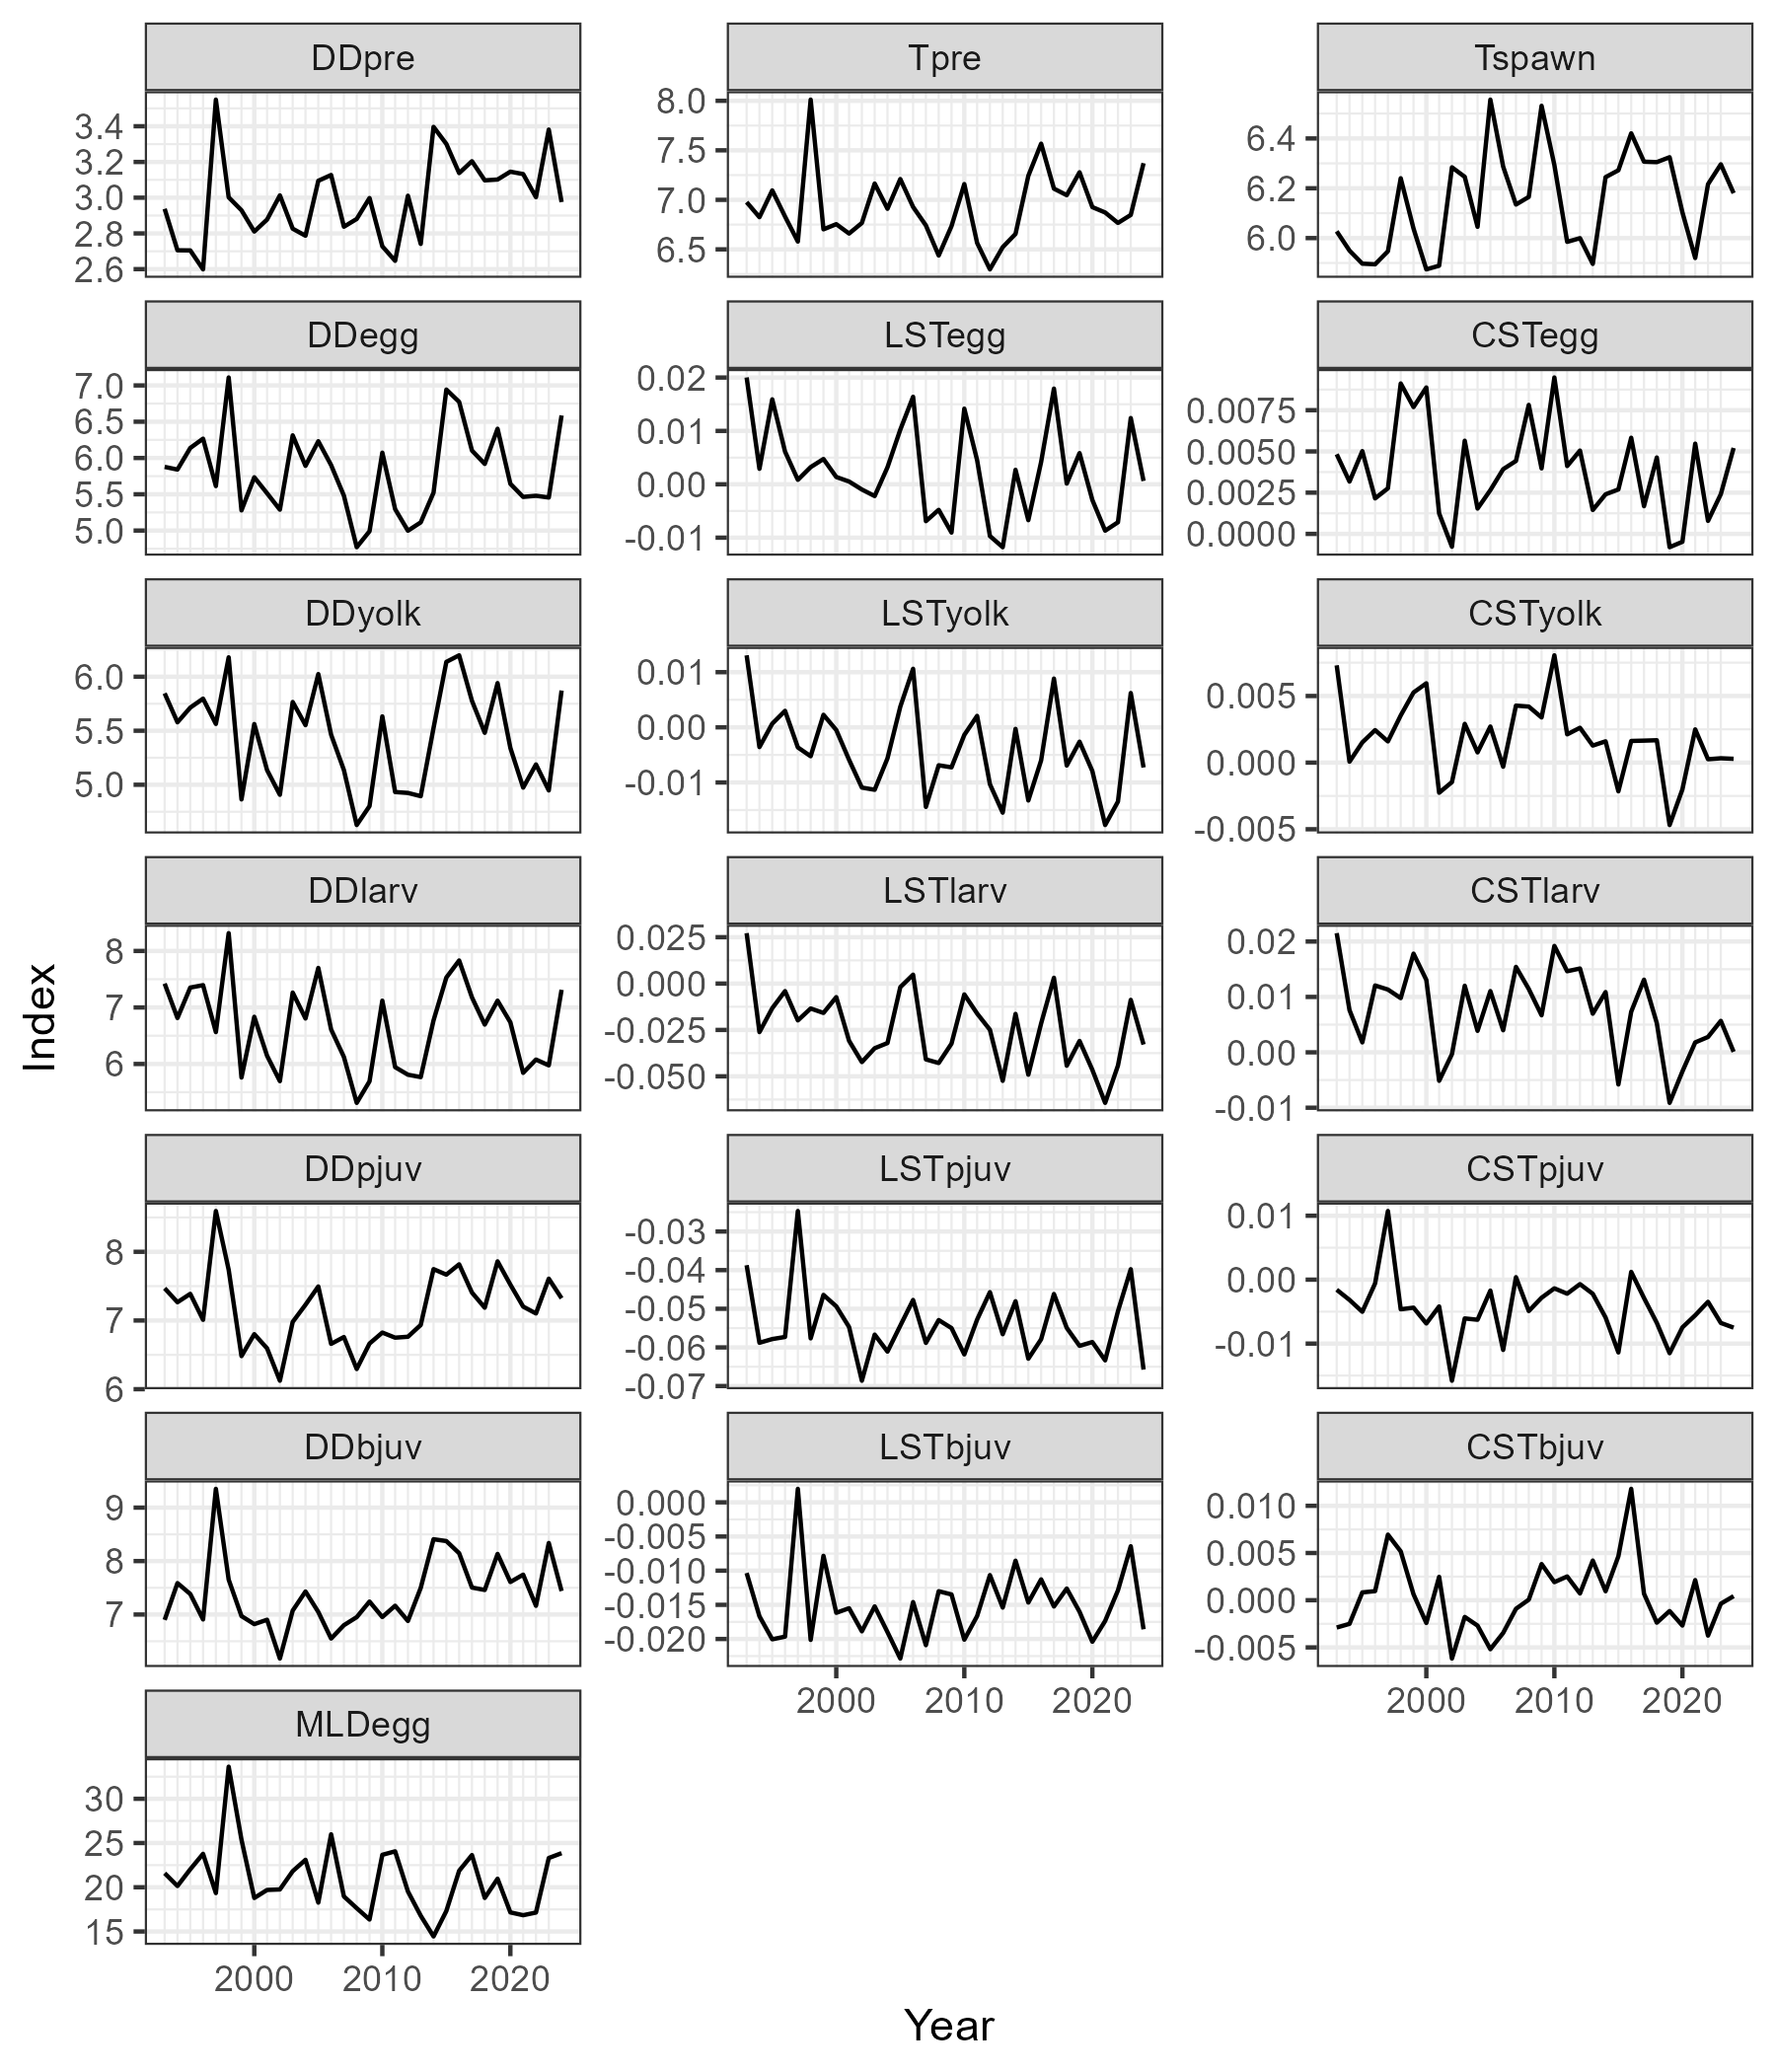
\includegraphics[width=6in,height=\textheight,keepaspectratio,alt={'Trend lines for each of the GLORYS time series. DD = degree days, T = temperature, MLD = mixed-layer depth, LST = longshore transport, CST = cross-shelf transport.'}]{figures/glorys_time_series.png}

}

\caption{\label{fig-glorys-ts-appendix}Transport and temperatures times
series from the GLORYS models. DD = degree days, T = temperature, MLD =
mixed-layer depth, LST = longshore transport, CST = cross-shelf
transport, pre = female precondition period prior to spawning, egg = egg
stage, larv = larval stage, pjuv = pelagic juveniles, bjuv = benthic
juveniles.}

\end{figure}%

\paragraph{Correlations among variables}\label{sec-corr}

GLORYS predictors were pre-screened for correlations among variables and
non-linear relationships with sablefish recruitment deviations.
Correlated predictors (r \(\ge\) 0.75,
Figure~\ref{fig-glorys-corr-appendix}) were excluded from the same
model.

\begin{figure}[H]

\centering{

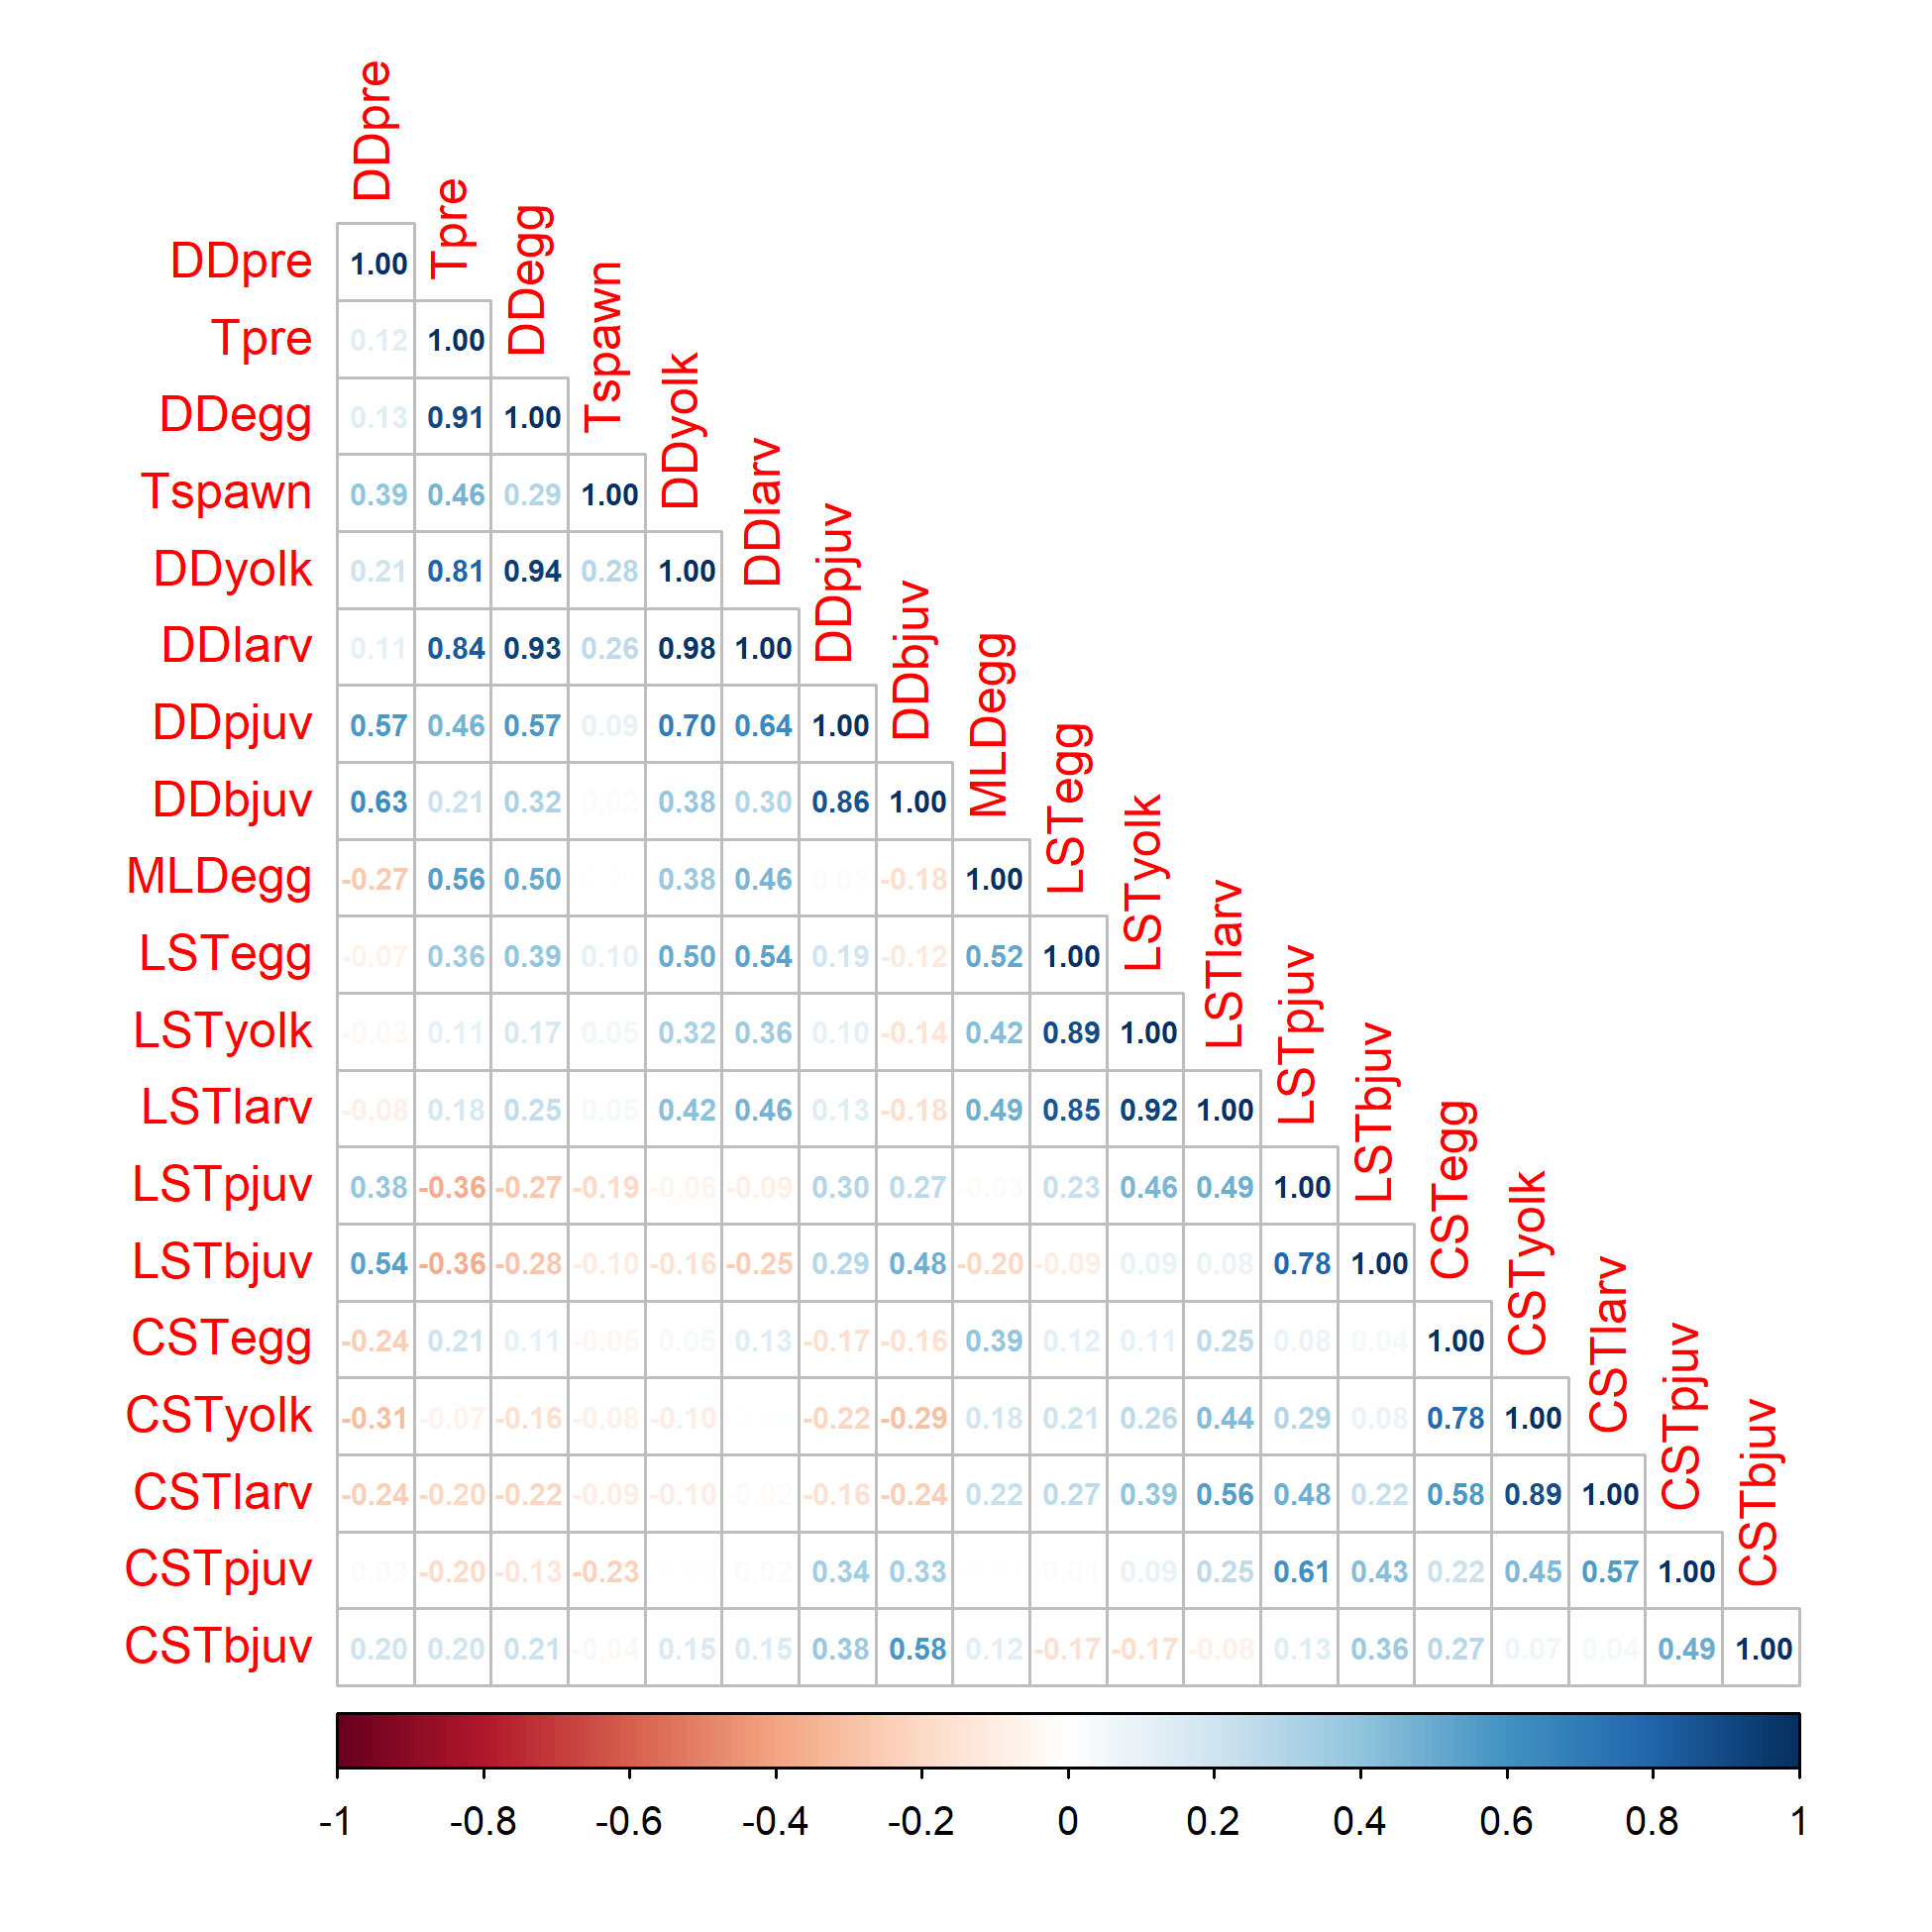
\includegraphics[width=6.5in,height=\textheight,keepaspectratio,alt={'Correlation matrix for the GLORYS time series. DD = degree days, T = temperature, MLD = mixed-layer depth, LST = longshore transport, CST = cross-shelf transport.'}]{figures/glorys-correlations-among-variables.png}

}

\caption{\label{fig-glorys-corr-appendix}Correlations between GLORYS
time series. DD = degree days, T = temperature, MLD = mixed-layer depth,
LST = longshore transport, CST = cross-shelf transport, pre = female
precondition period prior to spawning, egg = egg stage, larv = larval
stage, pjuv = pelagic juveniles, bjuv = benthic juveniles.}

\end{figure}%

\paragraph{Non-linear relationships}\label{sec-nonlin}

Non-linearity for individual terms was evaluated by comparing the linear
model to a model including both the linear and quadratic forms of the
predictor. If the AICc of the quadratic form was lower, we included the
quadratic form as a potential predictor as well, but required that the
linear term appear in models that included the quadratic from.

\subsubsection{Index development}\label{sec-indexdevel}

\paragraph{Methods}\label{methods}

We used linear models to examine relationships between ln(recruitment
deviations) from the 2023 sablefish stock assessment and predictors from
the GLOYRS model output. We used 1993-2019 as training data, leaving
2020-2024 as out-of-sample for use in the sensitivity analyses. We fit
all combinations of the GLORYS predictors, excluding correlated
variables from the same model, and limiting the the total number of
predictors in any model to three (just over 8 data points per
predictor). Model selection was carried out using the `dredge' function
in the MuMIn package in R (\citeproc{ref-MuMIn-cite}{Bartoń 2023};
\citeproc{ref-R-base}{R Core Team 2023}). Candidate models were
evaluated based on their \(\Delta\)AICc and number of predictors.

\begingroup
\fontsize{8.0pt}{9.0pt}\selectfont

\tagpdfsetup{table/header-rows={1}}
\begin{longtable}{lrrrrrrrrrrr}

\caption{\label{tbl-aic-appendix}Results of model fitting showing
estimated coefficients for models with delta AIC \textless/= 2.0. CST =
cross-shelf transport, DD = degree days, T = temperature, yolk =
yolksack stage, pjuv = pelagic juvenile, and bjuv = benthic juvenile
stage.}

\tabularnewline

\toprule
Model & Intercept & CSTbjuv & CSTegg & CSTpjuv & CSTyolk & DDpre & Tspawn & R2 & df & AICc & delta \\ 
\midrule\addlinespace[2.5pt]
Model 1 & 13.07 & 224.27 &  & -210.56 &  &  & -2.27 & 0.47 & 5 & 89.34 & 0.00 \\ 
Model 2 & 4.54 & 236.72 &  & -187.78 &  & -1.81 &  & 0.45 & 5 & 90.13 & 0.78 \\ 
Model 3 & -0.76 & 206.49 &  & -180.33 &  &  &  & 0.37 & 4 & 90.97 & 1.63 \\ 
Model 4 & -1.35 & 195.45 & 132.36 & -192.35 &  &  &  & 0.43 & 5 & 91.06 & 1.72 \\ 
Model 5 & -1.28 & 238.12 &  & -228.60 & 142.66 &  &  & 0.43 & 5 & 91.17 & 1.83 \\ 
\bottomrule

\end{longtable}

\endgroup

\paragraph{Results}\label{results}

Five models had \(\Delta\)AICc values \(\le\) 2.0
(Table~\ref{tbl-aic-appendix}). All models included cross-shelf
transport during pelagic juvenile (CSTpjuv), and benthic juvenile
(CSTbjuv) stages. Model 3 was chosen as the best-fit because it had the
fewest predictors (2), and these two predictors were in all top-five
models providing consistency. The best-fit model explained 37\% of the
variation in recruitment deviations from 1993-2022 (
r\textsuperscript{2} = 0.37 , Table~\ref{tbl-aic-appendix},
Figure~\ref{fig-glorys-fit-appendix}). The model tracked the data well
with most recruitment deviations falling with \(\pm\) 1.0 s.e. of the
recruitment index (Figure~\ref{fig-glorys-fit-appendix}).

The remaining four models included either Tspawn, DDpre, CSTegg, or
CSTyolk as predictors. These results suggest that different additional
terms might help explain variance in different years, but that CSTpjuv
and CSTbjuv provide a consistent basis for prediction. Including an
additional factor like Tpre would increase the explained variance by
\textasciitilde{} 10\% points (r\textsuperscript{2} = 0.47).

\begin{figure}[H]

\centering{

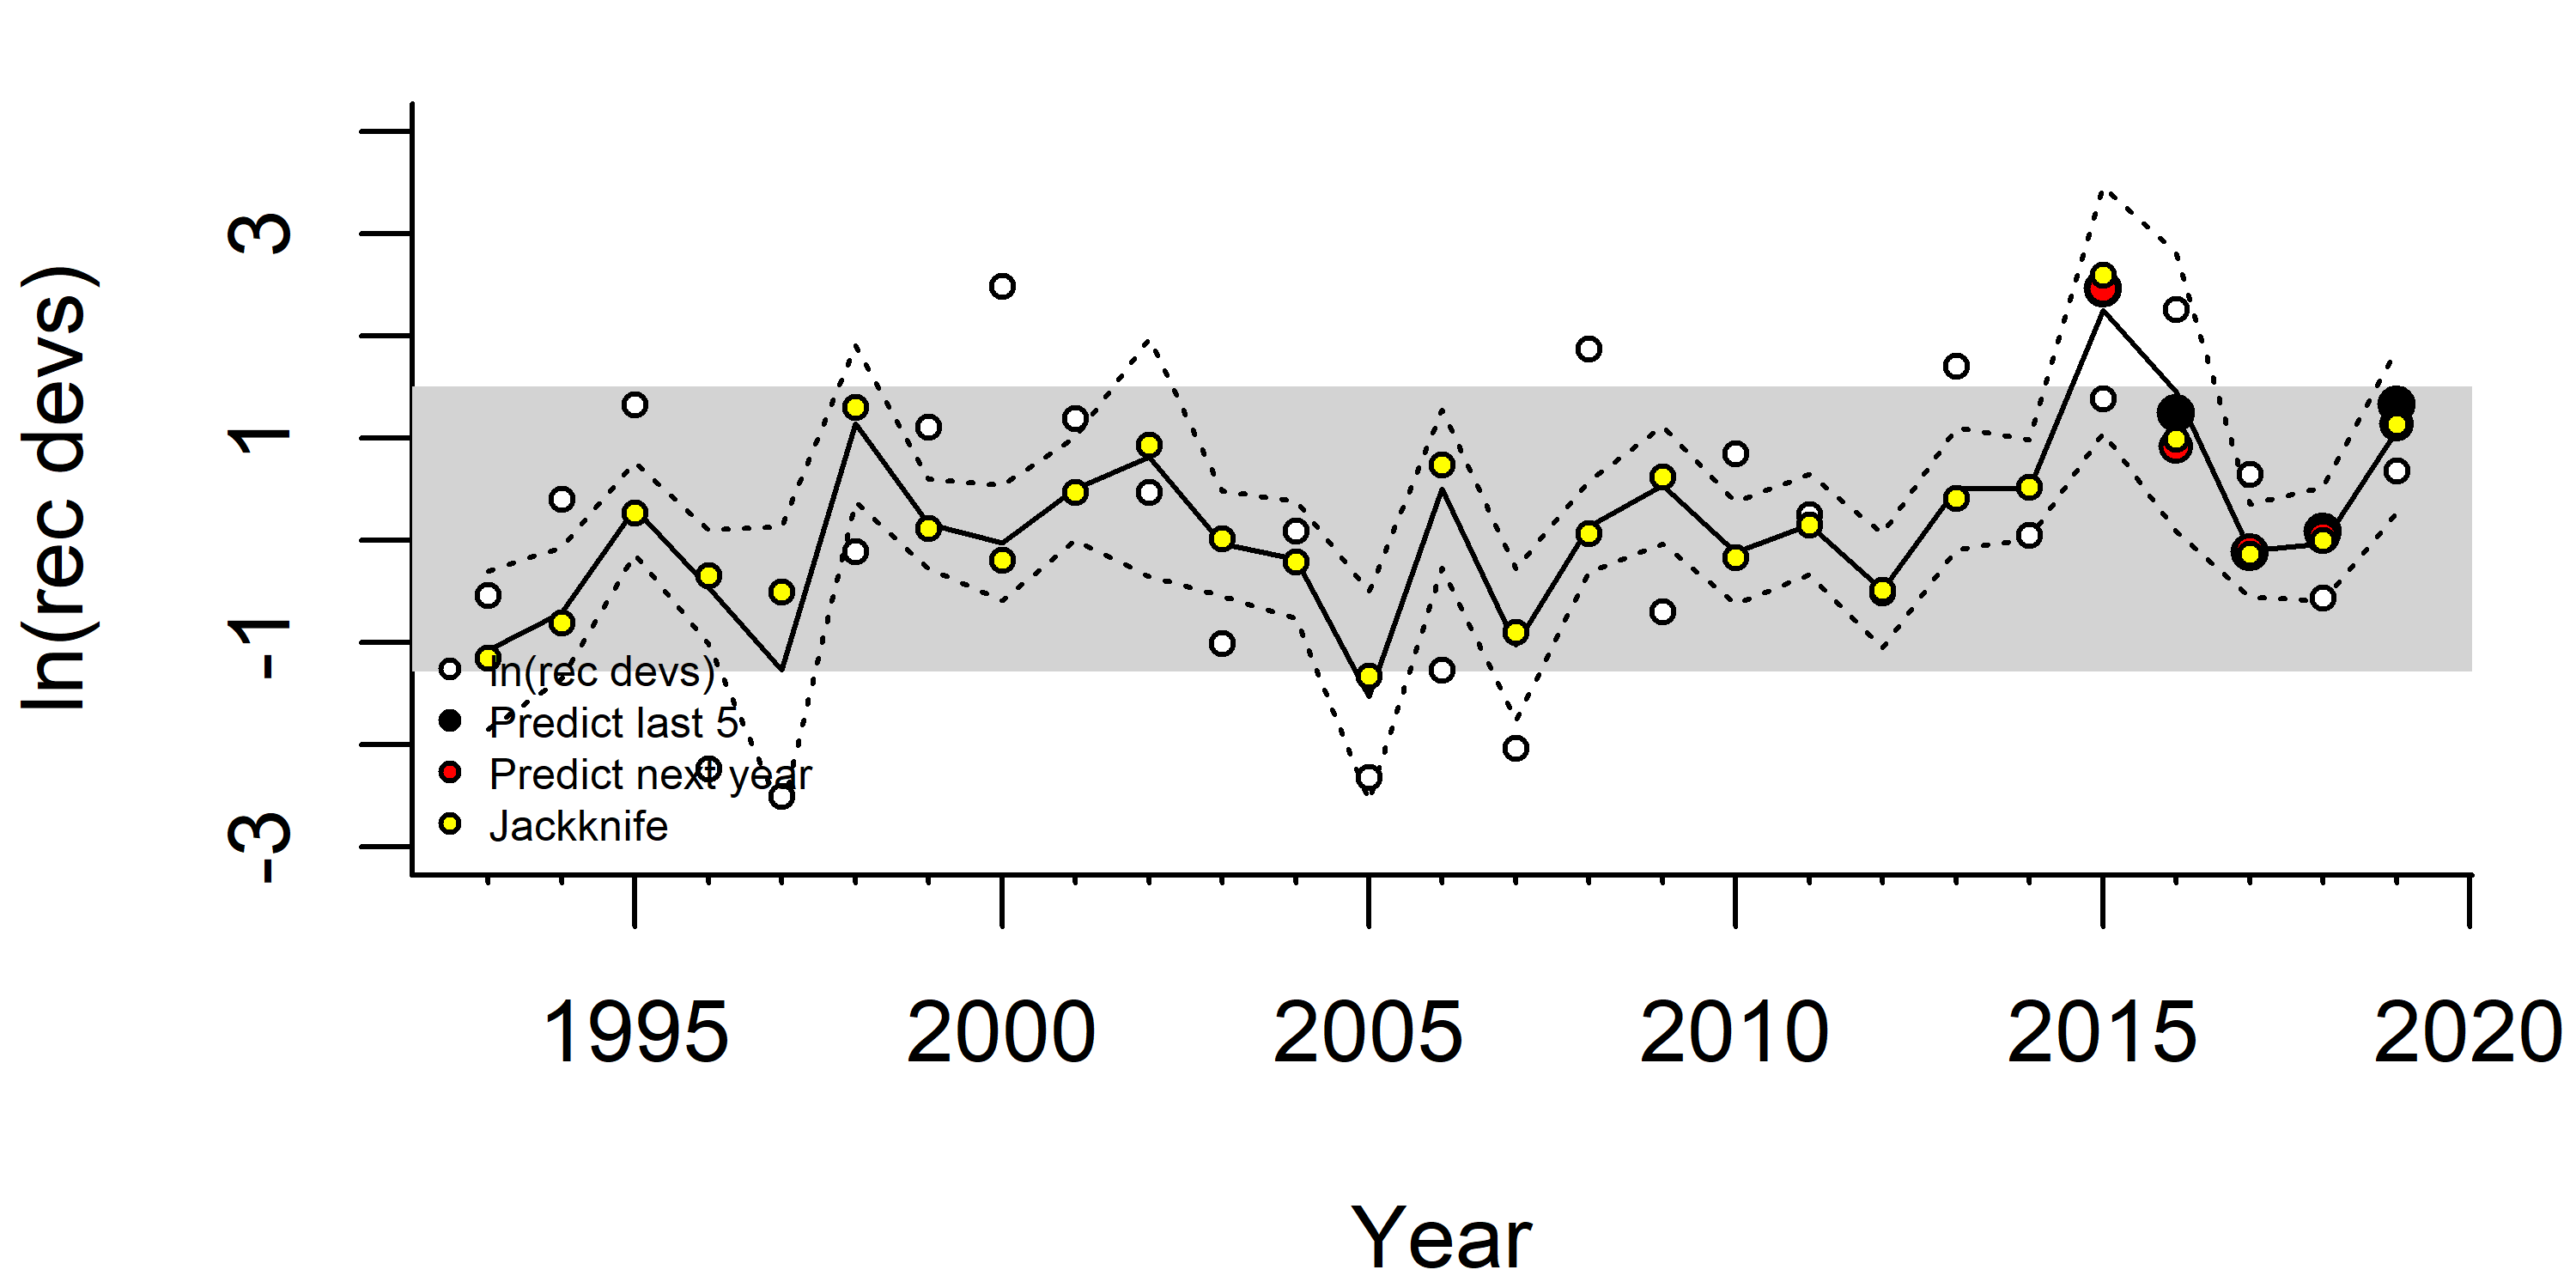
\includegraphics[width=0.9\linewidth,height=\textheight,keepaspectratio,alt={'Model fit to the training data (ln recruitment deviations from the stock assessment model for 1993-2019) and model testing results.'}]{figures/gloyrs_figure_3.png}

}

\caption{\label{fig-glorys-fit-appendix}Model fit to the training data
(ln recruitment deviations from the stock assessment model for
1993-2019) and model testing results. Black line is the model prediction
pm 1.0 s.e (dotted lines). Open (white) points are the ln recruitment
deviations. Yellow points are from jackknife analysis leaving out one
year and refitting the model, and red points fit the best-fit model to
1993-2014 then predict 2015-2019.}

\end{figure}%

For all models recruitment was negatively correlated with CSTpjuv
suggesting that processes like upwelling may be important for producing
feeding conditions conducive to survival. CSTbjuv was positively
correlated with recruitment, which may indicate that onshore transport
during the shift to benthic habitat leads to better recruitment. Both
the ROMS analysis and the results here suggest that colder water during
the female preconditioning stage (negative correlation with DDpre, here
model 2) results in higher recruitment.

\begin{figure}[H]

\centering{

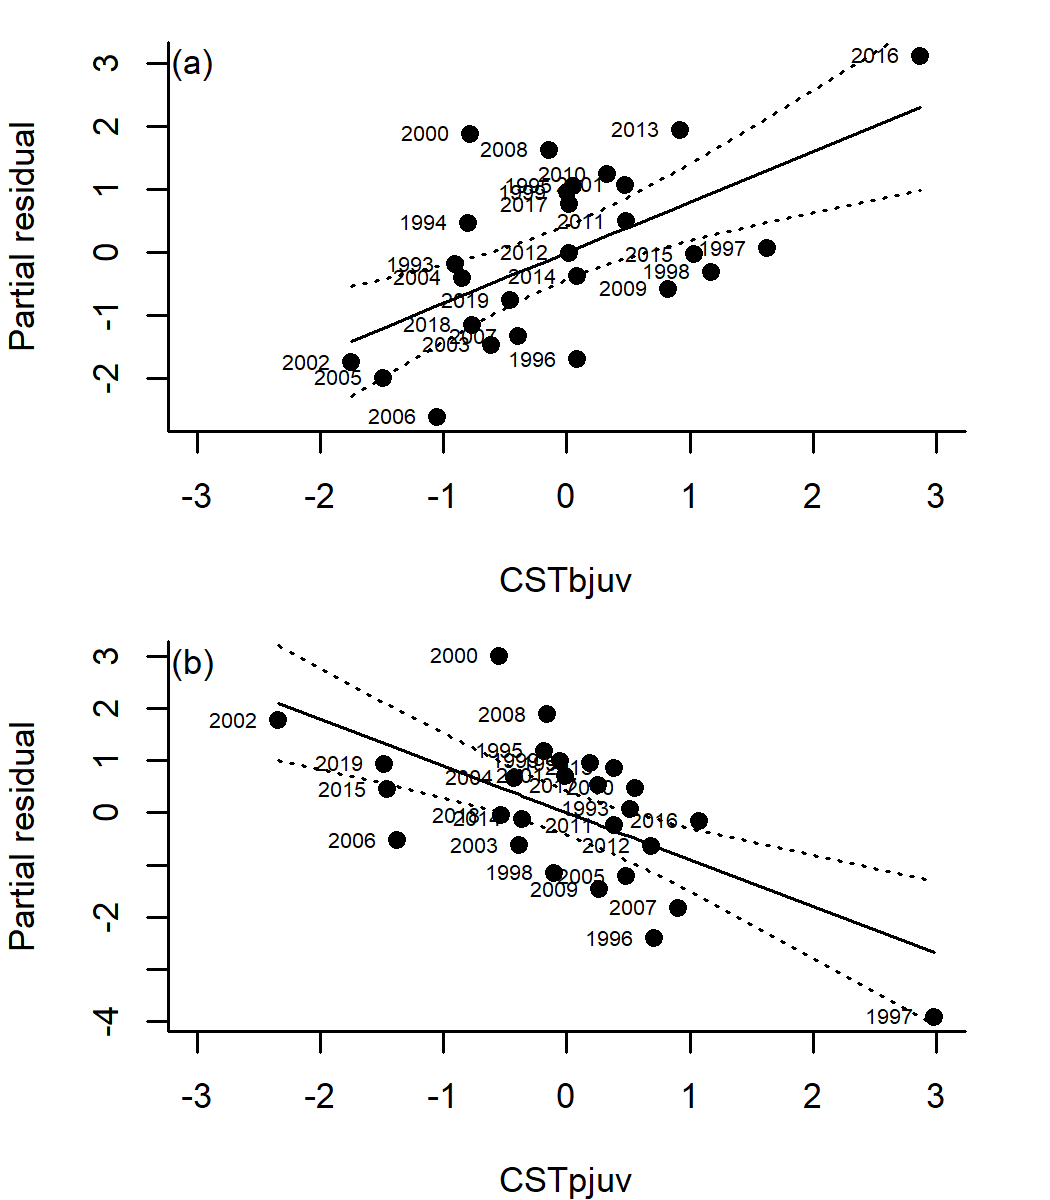
\includegraphics[width=0.9\linewidth,height=\textheight,keepaspectratio,alt={'Partial residual plots of GLORYS predictors. CST = cross-shelf transport, T = temperature, spawn = spaning stage, pjuv = pelagic juvenile, and bjuv = benthic juvenile stage.'}]{figures/gloyrs_figure_4.png}

}

\caption{\label{fig-glorys-terms-appendix}Partial residual plots of
GLORYS predictors. CST = cross-shelf transport, T = temperature, spawn =
spaning stage, pjuv = pelagic juvenile, and bjuv = benthic juvenile
stage.}

\end{figure}%

\paragraph{Model testing}\label{sec-modeltest}

Model diagnostics were examined and testing was carried out to determine
how stable the best-fit model was to both individual years and the
precision of the estimates of recruitment deviations. Testing followed
Tolimieri et al. (\citeproc{ref-tolimieri2018oceanographic}{2018}) and
Haltuch et al. (\citeproc{ref-haltuch2020oceanographic}{2020}), but only
a subset of test results is shown here:

\begin{enumerate}
\def\labelenumi{\arabic{enumi}.}
\item
  Jackknife analysis on the best-fit model was used to determine the
  impact of individual years on the model fit.
\item
  Refit the best-fit model using data for 1993-2014and then predict
  2015-2019.
\item
  Refit the best-fit model for 1993-2014 and predict 2015. Repeat
  stepping forward one year at a time.
\item
  Individual years were jackknifed and then the entire model selection
  process was rerun to determine the impact of individual years on the
  selection of the predictors in the best-fit model.
\end{enumerate}

Residual plots showed some deviation from the 1:1 line for the best-fit
model (Figure~\ref{fig-resids-appendix}).

\begin{figure}[H]

\centering{

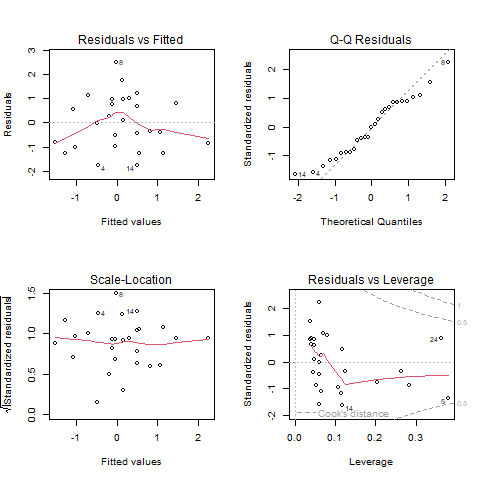
\includegraphics[width=0.9\linewidth,height=\textheight,keepaspectratio,alt={'Diagnostic plots from the best-fit model.'}]{figures/F_S1.diagnostic.plots.png}

}

\caption{\label{fig-resids-appendix}Diagnostics plots from the best-fit
model.}

\end{figure}%

Jackknife testing (excluding an individual year and refitting the
best-fit model) showed stable results with little change in the
r\textsuperscript{2} value (Figure~\ref{fig-glorys-fit-appendix} and
Figure~\ref{fig-jack-appendix}). Fitting the best-fit model to 1993-2014
and predicting 2015-2019 produced similar results to the best-fit model
(Figure~\ref{fig-glorys-fit-appendix}), as did predicting ahead one year
at a time from 2015 on.

\begin{figure}[H]

\centering{

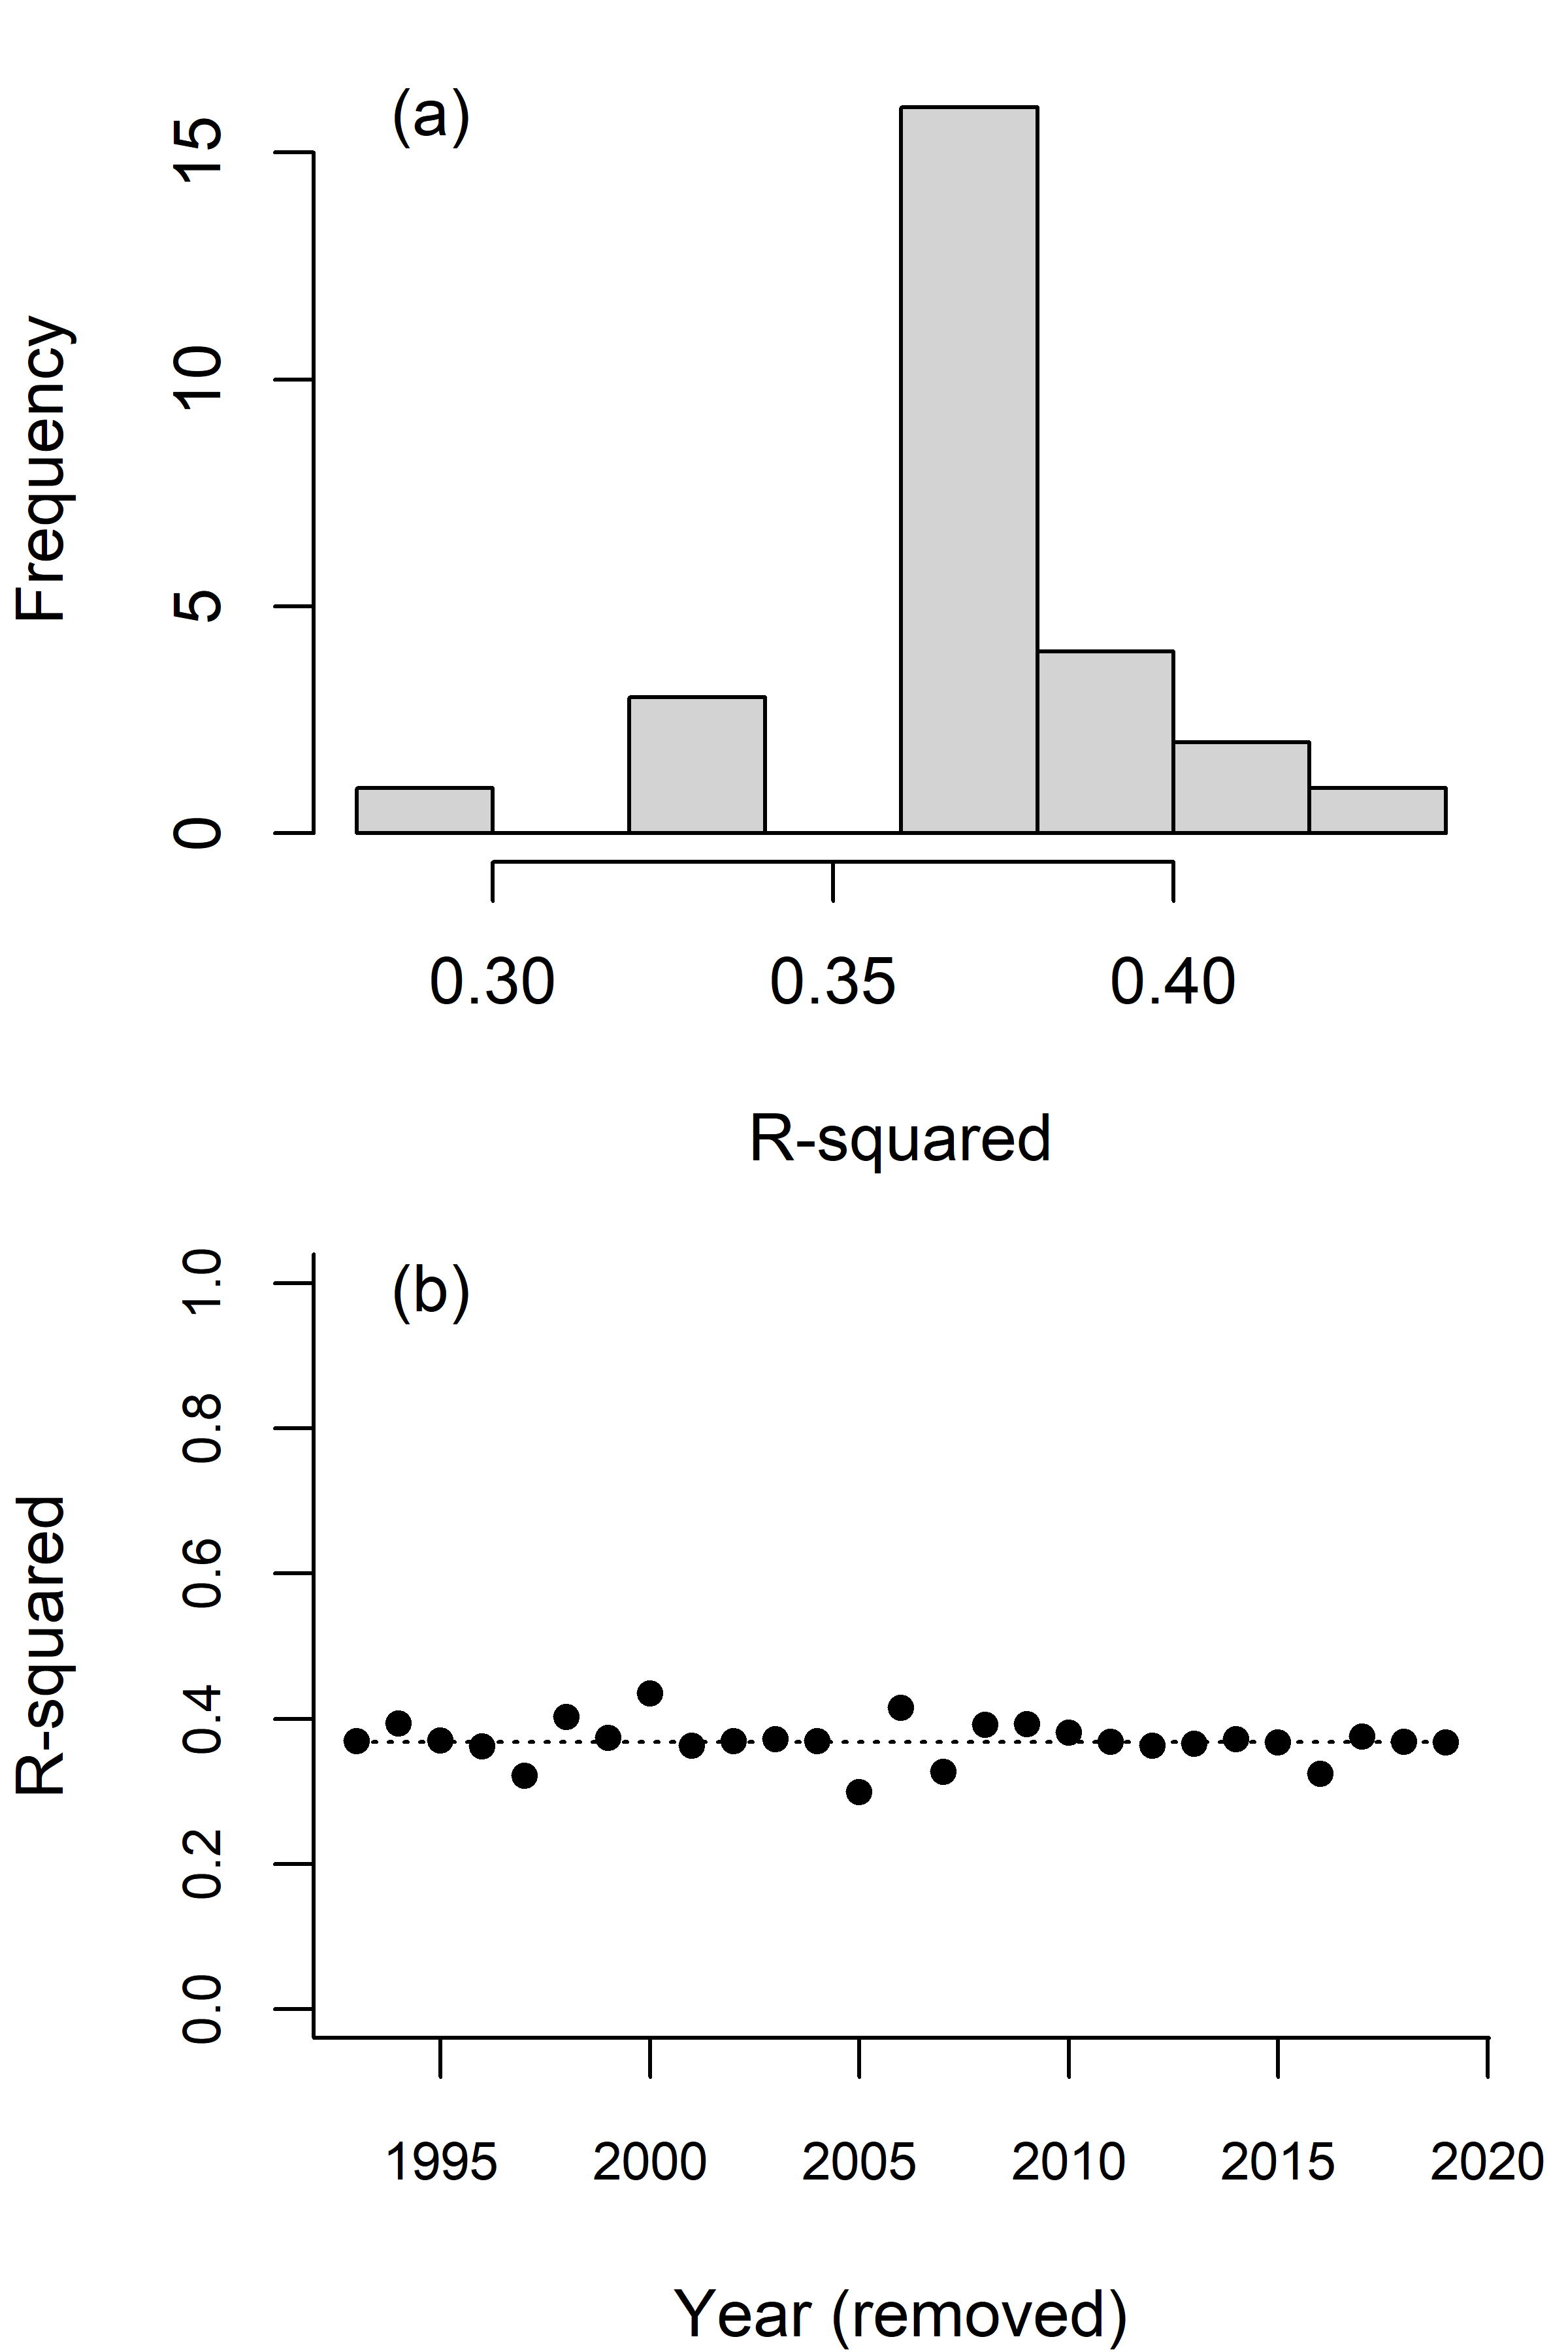
\includegraphics[width=0.9\linewidth,height=\textheight,keepaspectratio,alt={''}]{figures/Figure_5.png}

}

\caption{\label{fig-jack-appendix}Results of jackknife analysis
indicating changes in the r\textsuperscript{2} when individual years
were excluded from the best-fit model.}

\end{figure}%

Jackknifing individual years and re-running the entire model selection
produced stable model selection. CSTbjuv occurred in 28 of the 30 models
(where each model leave out one year); CSTpjuv was in 29 models; and
Tspawn was in 27 models. DDegg, CSTegg, and CSTlarv each occurred in one
model year.

\paragraph{Forward prediction}\label{sec-forwardpred}

GLORYS data were available through 2024, so we used the results of the
index fitting above to predict ln recruitment deviations from 2020 -
2024 (Figure~\ref{fig-predicted-recdevs-appendix}). The model predicted
average recruitment in 2020 and above average recruitment in 2021, 2023,
and 2024. The model picked up low recruitment in 2022, consistent with
the recruitment deviations from the 2023 assessment but under predicted
high recruitment in 2020, and 2021; thus the predictions were
conservative.

\begin{figure}[H]

\centering{

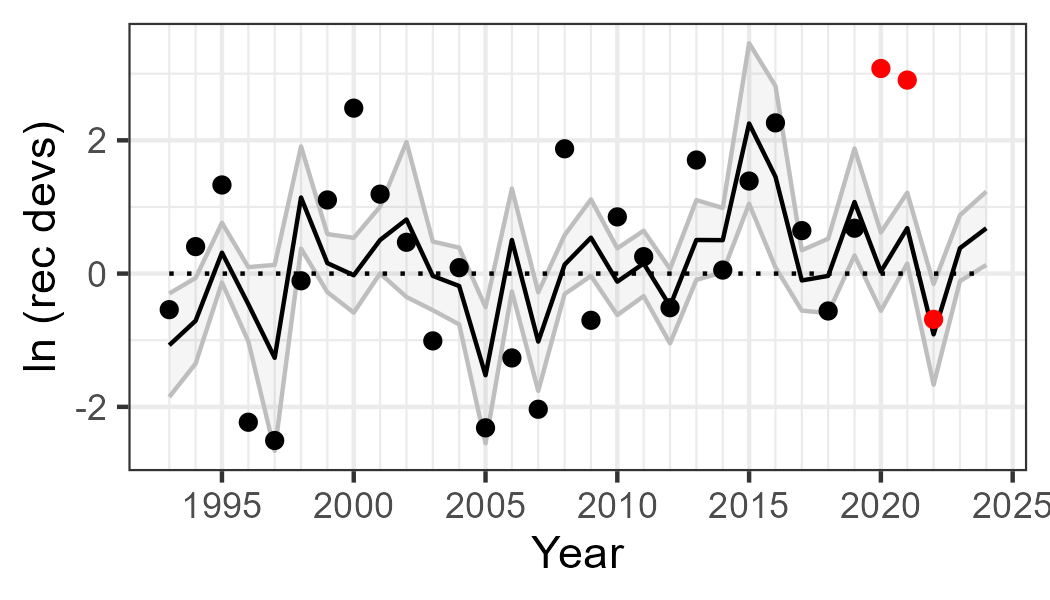
\includegraphics[width=0.9\linewidth,height=\textheight,keepaspectratio,alt={''}]{figures/gloyrs-predicted-recruitment-index.png}

}

\caption{\label{fig-predicted-recdevs-appendix}Predicted recruitment
deviations through 2024. Lines are the GLORYS index (predicted
recruitment through 2024) with standard error. The points are the ln
recruitment deviations from the 2023 assessment. Black points indicate
training data used in the initial model fitting. Red points are
out-of-sample data.}

\end{figure}%




\end{document}
